\documentclass[polish,]{book}
\usepackage[]{mathpazo}
\usepackage{amssymb,amsmath}
\usepackage{ifxetex,ifluatex}
\usepackage{fixltx2e} % provides \textsubscript
\ifnum 0\ifxetex 1\fi\ifluatex 1\fi=0 % if pdftex
  \usepackage[T1]{fontenc}
  \usepackage[utf8]{inputenc}
\else % if luatex or xelatex
  \ifxetex
    \usepackage{mathspec}
  \else
    \usepackage{fontspec}
  \fi
  \defaultfontfeatures{Ligatures=TeX,Scale=MatchLowercase}
\fi
% use upquote if available, for straight quotes in verbatim environments
\IfFileExists{upquote.sty}{\usepackage{upquote}}{}
% use microtype if available
\IfFileExists{microtype.sty}{%
\usepackage{microtype}
\UseMicrotypeSet[protrusion]{basicmath} % disable protrusion for tt fonts
}{}
\usepackage[margin=1in]{geometry}
\usepackage{hyperref}
\PassOptionsToPackage{usenames,dvipsnames}{color} % color is loaded by hyperref
\hypersetup{unicode=true,
            pdftitle={Na przełaj przez Data Mining z pakietem R},
            pdfauthor={Przemysław Biecek, Krzysztof Trajkowski},
            colorlinks=true,
            linkcolor=red,
            citecolor=red,
            urlcolor=blue,
            breaklinks=true}
\urlstyle{same}  % don't use monospace font for urls
\ifnum 0\ifxetex 1\fi\ifluatex 1\fi=0 % if pdftex
  \usepackage[shorthands=off,main=polish]{babel}
\else
  \usepackage{polyglossia}
  \setmainlanguage[]{polish}
\fi
\usepackage{natbib}
\bibliographystyle{apalike}
\usepackage{color}
\usepackage{fancyvrb}
\newcommand{\VerbBar}{|}
\newcommand{\VERB}{\Verb[commandchars=\\\{\}]}
\DefineVerbatimEnvironment{Highlighting}{Verbatim}{commandchars=\\\{\}}
% Add ',fontsize=\small' for more characters per line
\usepackage{framed}
\definecolor{shadecolor}{RGB}{248,248,248}
\newenvironment{Shaded}{\begin{snugshade}}{\end{snugshade}}
\newcommand{\AlertTok}[1]{\textcolor[rgb]{0.94,0.16,0.16}{#1}}
\newcommand{\AnnotationTok}[1]{\textcolor[rgb]{0.56,0.35,0.01}{\textbf{\textit{#1}}}}
\newcommand{\AttributeTok}[1]{\textcolor[rgb]{0.77,0.63,0.00}{#1}}
\newcommand{\BaseNTok}[1]{\textcolor[rgb]{0.00,0.00,0.81}{#1}}
\newcommand{\BuiltInTok}[1]{#1}
\newcommand{\CharTok}[1]{\textcolor[rgb]{0.31,0.60,0.02}{#1}}
\newcommand{\CommentTok}[1]{\textcolor[rgb]{0.56,0.35,0.01}{\textit{#1}}}
\newcommand{\CommentVarTok}[1]{\textcolor[rgb]{0.56,0.35,0.01}{\textbf{\textit{#1}}}}
\newcommand{\ConstantTok}[1]{\textcolor[rgb]{0.00,0.00,0.00}{#1}}
\newcommand{\ControlFlowTok}[1]{\textcolor[rgb]{0.13,0.29,0.53}{\textbf{#1}}}
\newcommand{\DataTypeTok}[1]{\textcolor[rgb]{0.13,0.29,0.53}{#1}}
\newcommand{\DecValTok}[1]{\textcolor[rgb]{0.00,0.00,0.81}{#1}}
\newcommand{\DocumentationTok}[1]{\textcolor[rgb]{0.56,0.35,0.01}{\textbf{\textit{#1}}}}
\newcommand{\ErrorTok}[1]{\textcolor[rgb]{0.64,0.00,0.00}{\textbf{#1}}}
\newcommand{\ExtensionTok}[1]{#1}
\newcommand{\FloatTok}[1]{\textcolor[rgb]{0.00,0.00,0.81}{#1}}
\newcommand{\FunctionTok}[1]{\textcolor[rgb]{0.00,0.00,0.00}{#1}}
\newcommand{\ImportTok}[1]{#1}
\newcommand{\InformationTok}[1]{\textcolor[rgb]{0.56,0.35,0.01}{\textbf{\textit{#1}}}}
\newcommand{\KeywordTok}[1]{\textcolor[rgb]{0.13,0.29,0.53}{\textbf{#1}}}
\newcommand{\NormalTok}[1]{#1}
\newcommand{\OperatorTok}[1]{\textcolor[rgb]{0.81,0.36,0.00}{\textbf{#1}}}
\newcommand{\OtherTok}[1]{\textcolor[rgb]{0.56,0.35,0.01}{#1}}
\newcommand{\PreprocessorTok}[1]{\textcolor[rgb]{0.56,0.35,0.01}{\textit{#1}}}
\newcommand{\RegionMarkerTok}[1]{#1}
\newcommand{\SpecialCharTok}[1]{\textcolor[rgb]{0.00,0.00,0.00}{#1}}
\newcommand{\SpecialStringTok}[1]{\textcolor[rgb]{0.31,0.60,0.02}{#1}}
\newcommand{\StringTok}[1]{\textcolor[rgb]{0.31,0.60,0.02}{#1}}
\newcommand{\VariableTok}[1]{\textcolor[rgb]{0.00,0.00,0.00}{#1}}
\newcommand{\VerbatimStringTok}[1]{\textcolor[rgb]{0.31,0.60,0.02}{#1}}
\newcommand{\WarningTok}[1]{\textcolor[rgb]{0.56,0.35,0.01}{\textbf{\textit{#1}}}}
\usepackage{longtable,booktabs}
\usepackage{graphicx,grffile}
\makeatletter
\def\maxwidth{\ifdim\Gin@nat@width>\linewidth\linewidth\else\Gin@nat@width\fi}
\def\maxheight{\ifdim\Gin@nat@height>\textheight\textheight\else\Gin@nat@height\fi}
\makeatother
% Scale images if necessary, so that they will not overflow the page
% margins by default, and it is still possible to overwrite the defaults
% using explicit options in \includegraphics[width, height, ...]{}
\setkeys{Gin}{width=\maxwidth,height=\maxheight,keepaspectratio}
\setlength{\emergencystretch}{3em}  % prevent overfull lines
\providecommand{\tightlist}{%
  \setlength{\itemsep}{0pt}\setlength{\parskip}{0pt}}
\setcounter{secnumdepth}{5}
% Redefines (sub)paragraphs to behave more like sections
\ifx\paragraph\undefined\else
\let\oldparagraph\paragraph
\renewcommand{\paragraph}[1]{\oldparagraph{#1}\mbox{}}
\fi
\ifx\subparagraph\undefined\else
\let\oldsubparagraph\subparagraph
\renewcommand{\subparagraph}[1]{\oldsubparagraph{#1}\mbox{}}
\fi

%%% Use protect on footnotes to avoid problems with footnotes in titles
\let\rmarkdownfootnote\footnote%
\def\footnote{\protect\rmarkdownfootnote}

%%% Change title format to be more compact
\usepackage{titling}

% Create subtitle command for use in maketitle
\providecommand{\subtitle}[1]{
  \posttitle{
    \begin{center}\large#1\end{center}
    }
}

\setlength{\droptitle}{-2em}

  \title{Na przełaj przez Data Mining z pakietem R}
    \pretitle{\vspace{\droptitle}\centering\huge}
  \posttitle{\par}
    \author{Przemysław Biecek, Krzysztof Trajkowski}
    \preauthor{\centering\large\emph}
  \postauthor{\par}
      \predate{\centering\large\emph}
  \postdate{\par}
    \date{2019-04-11}

\usepackage{booktabs}
\usepackage{booktabs}
\usepackage{longtable}
\usepackage{array}
\usepackage{multirow}
\usepackage{wrapfig}
\usepackage{float}
\usepackage{colortbl}
\usepackage{pdflscape}
\usepackage{tabu}
\usepackage{threeparttable}
\usepackage{threeparttablex}
\usepackage[normalem]{ulem}
\usepackage{makecell}
\usepackage{xcolor}

\begin{document}
\maketitle

{
\hypersetup{linkcolor=black}
\setcounter{tocdepth}{2}
\tableofcontents
}
\hypertarget{part_1}{%
\chapter{Kilka słów zamiast wstępu}\label{part_1}}

\begin{quote}
\emph{na przełaj ``najkrótszą drogą, nie trzymając się wytycznej trasy''}

--- Słownik Języka Polskiego PWN
\end{quote}

\begin{quote}
\emph{``Kto chodzi na skróty, ten nie śpi w domu''}

--- Mądrość ludowa ;-)
\end{quote}

\begin{quote}
\emph{``Nie ma drogi na skróty, do miejsca do którego, warto dojść''}

--- Edith
\end{quote}

W połowie roku 2010 te notatki zostały ``otwarte''. Osoby chcące je rozwijać
są do tego gorąco zachęcane. Poniżej znajduje się aktualna lista autorów kolejnych
rozdziałów:

\begin{itemize}
\item
  Rozdziały 2 do 6 przygotowuje Przemek Biecek

  . \href{mailto:przemyslaw.biecek@gmail.com}{\nolinkurl{przemyslaw.biecek@gmail.com}}
\item
  Rozdziały 7 do 13 przygotowuje Krzysiek Trajkowski

  . \href{mailto:seaproject@poczta.onet.pl}{\nolinkurl{seaproject@poczta.onet.pl}}
\end{itemize}

Notatki zatytułowane „na przełaj'' przygotowane są jako materiały pomocnicze.
Każdy może z nich korzystać, pamiętając jednak że:

\begin{itemize}
\item
  Notatki zostały przygotowane tak, bym ułatwić wykonywanie pewnych analiz
  w R, nacisk został położony na poznanie pakietu R jako narzędzia do wykonywania danych analiz.
\item
  Notatki NIE ZOSTAŁY przygotowane tak by uczyć się z nich metodologii.
  NIE SĄ tutaj dyskutowane zagadnienia teoretyczne, nie ma tu wyprowadzeń,
  nie ma sprawdzenia niektórych założeń. Od tego są książki, staram się w bibliografii zamieszać lepsze pozycje które udało mi się znaleźć.
\item
  Notatki przygotowuję ucząc się danych metod, NIE SĄ więc to materiały zebrane przez eksperta, czasami nie są to nawet materiały czytane po raz drugi.
  Chętnie usłyszę co w takich notatkach powinno się znaleźć dodatkowo, co jest
  niejasne lub co jest błędem tak merytorycznym jak i językowym.
\end{itemize}

Analiza danych to nie tylko klasyczna statystyka z zagadnieniami estymacji i testowania (najczęściej wykładanymi na standardowych kursach statystyki). Znaczny
zbiór metod analizy danych nazywany technikami eksploracji danych lub data mining dotyczy zagadnień klasyfikacji, identyfikacji, analizy skupień oraz modelowania
złożonych procesów. Właśnie te metody będą nas interesować w poniższym rozdziale.

Data mining to szybko rosnąca grupa metod analizy danych rozwijana nie tylko
przez statystyków ale głównie przez biologów, genetyków, cybernetyków, informatyków, ekonomistów, osoby pracujące nad rozpoznawaniem obrazów, myśli i wiele
innych grup zawodowych. Podobnie jak w poprzednich rozdziałach nie będziemy dokładnie omawiać poszczególnych algorytmów ani szczegółowo dyskutować kontekstu
aplikacyjnego danej metody. Zakładamy, że czytelnik zna te metody, zna ich założenia i podstawy teoretyczne ale jest zainteresowany w jakich funkcjach pakietu R
są one zaimplementowane. Stąd też skrótowe traktowanie wielu zagadnień. Osoby
szukające więcej informacji o sposobie działania poszczególnych algorytmów znajdą
z pewnością wiele pozycji poświęconym konkretnym metodom, szczególnie polecam
książki \citep{KC2005} oraz \citep{HTF2001}.

Przedstawione metody zostały podzielone na trzy grupy. Pierwsza z nich to metody związane z zagadnieniem redukcji wymiaru. Te metody są również wykorzystywane do ekstrakcji cech oraz do wstępnej obróbki danych, stanowią więc często
etap pośredni w analizach. Druga grupa metod związana jest z zagadnieniem analizy
skupień (w innej nomenklaturze nazywanym uczeniem bez nadzoru). Przedstawiane będą metody hierarchiczne oraz grupujące. Ostatnia grupa metod związana jest
z zagadnieniem dyskryminacji (w innej nomenklaturze - uczeniem pod nadzorem lub
klasyfikacją).

\hypertarget{part_2}{%
\chapter{Redukcja wymiaru}\label{part_2}}

Metody redukcji wymiaru umożliwiają przedstawienie obserwacji w przestrzeni o
zadanym wymiarze, niższym niż w przypadku oryginalnych danych.

Przedstawimy wybrane metody na przykładzie danych z różnych województw
(zbiór danych \texttt{daneGUS}, patrz ostatni rozdział). Dla każdego z województw zebrano informację o liczbie studentów w tych województwach w rozbiciu na 16 grup
kierunków. Każde województwo jest więc opisane wektorem 16 liczb.

Przypuśćmy, że chcemy przedstawić graficznie te województwa. Jak uwzględnić
wszystkie 16 parametrów? Jednym z rozwiązań jest użycie metod redukcji wymiaru i
liczby zmiennych z 16 do 2. Opisanie każdego z województw dwoma liczbami ułatwi
przedstawianie graficzne tych województw.

Więc do dzieła!

Redukcja wymiaru często jest pośrednim etapem w zagadnieniu klasyfikacji, analizy skupień czy regresji. W określonych sytuacjach pozwala na poprawę skuteczności
tych metod, zwiększa stabilność a czasem pozwala na uwzględnienie w analizach dużej liczby zmiennych. Jest też popularnie wykorzystywaną metodą do wizualizacji
wielowymiarowych zmiennych, dane są redukowane do przestrzeni dwuwymiarowej,
w której już łatwo je przedstawić na wykresie. Metody z tej grupy są również nazywane metodami ekstrakcji cech, ponieważ w wyniku redukcji wymiaru tworzone są
nowe cechy, które mogą być wykorzystane do innych zagadnień.

\hypertarget{part_21}{%
\section{Analiza składowych głównych (PCA, ang. Principal Components Analysis)}\label{part_21}}

Analiza składowych głównych służy do wyznaczania nowych zmiennych, których
możliwie mały podzbiór będzie mówił możliwie dużo o całej zmienności w zbiorze
danych. Nowy zbiór zmiennych będzie tworzył bazę ortogonalną w przestrzeni cech.
Zmienne będą wybierane w ten sposób by pierwsza zmienna odwzorowywała możliwie dużo zmienności w danych (po zrzutowaniu obserwacji na ten wektor, chcemy by
wariancja rzutów była najwyższa). Po wyznaczeniu pierwszej zmiennej wyznaczamy
drugą, tak by była ortogonalna do pierwszej, i wyjaśniała możliwie dużo pozostałej
zmienności, kolejną zmienną wybieramy tak by była ortogonalna do dwóch pierwszych itd.

Tak uzyskany zbiór wektorów tworzy bazę ortogonalną w przestrzeni cech, a co
więcej pierwsze współrzędne wyjaśniają większość zmienności w obserwacjach. Celem metody składowych głównych jest więc znalezienie transformacji układu współrzędnych, która lepiej opisze zmienność pomiędzy obserwacjami. Przykład takiej
transformacji pokazujemy na rysunku \ref{fig:PCA}. Przedstawiamy obserwacje w oryginalnym układzie współrzędnych (lewy rysunek) i w nowym układzie współrzędnych
(prawy rysunek).

\begin{figure}

{\centering \includegraphics[width=1\linewidth]{PCAprzykald} 

}

\caption{Przykład transformacji zmiennych z użyciem metody PCA.}\label{fig:PCA}
\end{figure}

W pakiecie R dostępnych jest kilka implementacji metody składowych głównych.
Przedstawione poniżej najpopularniejsze wersje znajdują się w funkcjach \href{https://rdrr.io/r/stats/prcomp.html}{\texttt{prcomp(stats)}}
i \href{https://rdrr.io/r/stats/princomp.html}{\texttt{princomp(stats)}} z pakietu \href{https://rdrr.io/r/\#stats}{\texttt{stats}}. Inne popularne wersje znaleźć można w funkcjach \href{https://rdrr.io/cran/FactoMineR/man/PCA.html}{\texttt{PCA(FactoMineR)}}, \href{https://rdrr.io/r/stats/cmdscale.html}{\texttt{cmdscale(stats)}} lub \texttt{pca(pcurve)}.

Poszczególne implementacje różnią się metodami wykorzystanymi do znalezienia
nowego układu zmiennych. W przypadku funkcji \href{https://rdrr.io/r/stats/princomp.html}{prcomp()} nowe zmienne wyznaczane są z z użyciem dekompozycji na wartości osobliwe SVD. Ten sposób wyznaczania
składowych głównych jest zalecany z uwagi na dużą dokładność numeryczną. W
funkcji \href{https://rdrr.io/r/stats/princomp.html}{princomp()} składowe główne są wyznaczane poprzez wektory własne macierzy kowariancji pomiędzy zmiennymi, używana jest więc dekompozycja spektralna.
Teoretyczne właściwości wyznaczonych składowych głównych będą identyczne, jednak w określonych sytuacjach otrzymane wyniki dla poszczególnych funkcji mogą
się różnić.

Poniższy kod pokazuje w jaki sposób działa funkcja \href{https://rdrr.io/r/stats/princomp.html}{princomp()}. Wyznaczane
są wektory własne macierzy kowariancji, tworzą one macierz przekształcenia dla
danych.

\begin{verbatim}
kowariancja = cov(dane)
eig = eigen(kowariancja)
noweDane = dane %*% eig$vectors
\end{verbatim}

Poniższy kod pokazuje w jaki sposób działa funkcja \texttt{prcomp()}. Wykorzystywana
jest dekompozycja SVD.

\begin{verbatim}
svdr = svd(dane)
noweDane = dane %*% svdr$v
\end{verbatim}

Obu funkcji do wyznaczania składowych głównych używa się w podobny sposób,
kolejne argumenty określają zbiór danych (można wskazać macierz, ramkę danych,
lub formułę określającą które zmienne mają być transformowane) oraz informacje
czy zmienne powinny być uprzednio wycentrowane i przeskalowane. To czy dane
przed wykonaniem analizy składowych głównych mają być przeskalowane zależy od
rozwiązywanego problemu, w większości sytuacji skalowanie pozwala usunąć wpływ
takich artefaktów jak różne jednostki dla poszczególnych zmiennych. W obiektach
przekazywanych jako wynik przez obie funkcje przechowywane są podobne informa-
cje, choć w polach o różnej nazwie. Wynikiem funkcji \href{https://rdrr.io/r/stats/princomp.html}{\texttt{prcomp()}} jest obiekt klasy
\texttt{prcomp}, którego pola są wymienione w tabeli \ref{tab:tab01}.

\begin{table}[t]

\caption{\label{tab:tab01}Pola obiektu klasy $\texttt{prcomp}$.}
\centering
\begin{tabular}{>{}l||>{\raggedright\arraybackslash}p{35em}}
\hline
. & opis\\
\hline
$\texttt{\$sdev}$ & Wektor odchyleń standardowych dla obserwacji. Kolejne zmienne odpowiadają odchyleniom standardowym liczonym dla kolejnych składowych głównych.\\
\hline
$\texttt{\$rotation}$ & Macierz obrotu przekształcająca oryginalny układ współrzędnych w nowy układ współrzędnych.\\
\hline
$\texttt{\$center}$ & Wektor wartości wykorzystanych przy centrowaniu obserwacji.\\
\hline
$\texttt{\$scale}$ & Wektor wartości wykorzystanych przy skalowaniu obserwacji.\\
\hline
$\texttt{\$x}$ & Macierz współrzędznych kolejnych obserwacji w nowym
układzie współrzędnych, macierz ta ma identyczne wymiary co oryginalny zbiór zmiennych.\\
\hline
\end{tabular}
\end{table}

Dla obiektów klasy prcomp dostępne są przeciążone wersje funkcji \texttt{plot()}, \texttt{summary()},
\texttt{biplot()}. Poniżej przedstawiamy przykładowe wywołanie tych funkcji. Graficzny
wynik ich działania jest przedstawiony na rysunku \ref{fig:wy212}. Lewy rysunek przedstawia
wynik dla funkcji \texttt{plot()} a prawy przedstawia wynik funkcji \texttt{biplot()} wykonanych
dla argumentu klasy \texttt{prcomp}. Na lewym rysunku przedstawione są wariancje wyjaśnione przez kolejne wektory nowego układu współrzędnych. Ta informacja jest
podawana również przez funkcje \texttt{summary()}. Prawy rysunek przedstawia biplot, na
którym umieszczone są dwa wykresy. Jeden przedstawia indeksy obserwacji przedstawione na układzie współrzędnych określonych przez dwie pierwsze składowe główne
(w tym przypadku dwie współrzędne wyjaśniają około \(50\%\) całej zmienności). Drugi
rysunek przedstawia kierunki w których działają oryginalne zmienne, innymi słowy
przedstawiają jak wartość danej zmiennej wpływa na wartości dwóch pierwszych
składowych głównych.

Jeżeli wektory mają przeciwne zwroty to dane zmienne są ujemnie skorelowane
(nie można jednak ocenić wartości korelacji), jeżeli zwroty są prostopadłe to zmienne są nieskorelowane, a jeżeli zwroty są bliskie to zmienne są dodatnio skorelowane.

\begin{Shaded}
\begin{Highlighting}[]
\NormalTok{daneO <-}\StringTok{ }\KeywordTok{read.table}\NormalTok{(}\StringTok{"http://www.biecek.pl/R/dane/daneO.csv"}\NormalTok{,}\DataTypeTok{sep=}\StringTok{";"}\NormalTok{,}\DataTypeTok{header =} \OtherTok{TRUE}\NormalTok{)}
\CommentTok{# przygotowujemy dane, usuwamy zmienne jakościowe i brakujące przypadki}
\NormalTok{dane =}\StringTok{ }\KeywordTok{na.omit}\NormalTok{(daneO[,}\OperatorTok{-}\KeywordTok{c}\NormalTok{(}\DecValTok{4}\NormalTok{,}\DecValTok{5}\NormalTok{,}\DecValTok{6}\NormalTok{,}\DecValTok{7}\NormalTok{)])}
\CommentTok{# wykonujemy analizę składowych głównych, normalizując wcześniej zmienne}
\NormalTok{wynik =}\StringTok{ }\KeywordTok{prcomp}\NormalTok{(dane, }\DataTypeTok{scale=}\NormalTok{T)}
\CommentTok{# jak wygląda obiekt z wynikami od środka}
\KeywordTok{str}\NormalTok{(wynik)}
\end{Highlighting}
\end{Shaded}

\begin{verbatim}
## List of 5
##  $ sdev    : num [1:5] 1.153 1.068 0.963 0.916 0.873
##  $ rotation: num [1:5, 1:5] 0.5016 0.0935 -0.4244 0.4878 -0.5671 ...
##   ..- attr(*, "dimnames")=List of 2
##   .. ..$ : chr [1:5] "Wiek" "Rozmiar.guza" "Wezly.chlonne" "Okres.bez.wznowy" ...
##   .. ..$ : chr [1:5] "PC1" "PC2" "PC3" "PC4" ...
##  $ center  : Named num [1:5] 45.417 1.271 0.417 37.406 2640.896
##   ..- attr(*, "names")= chr [1:5] "Wiek" "Rozmiar.guza" "Wezly.chlonne" "Okres.bez.wznowy" ...
##  $ scale   : Named num [1:5] 6.206 0.447 0.496 9.527 3616.045
##   ..- attr(*, "names")= chr [1:5] "Wiek" "Rozmiar.guza" "Wezly.chlonne" "Okres.bez.wznowy" ...
##  $ x       : num [1:96, 1:5] -1.5446 0.0105 -1.4565 -1.2352 -1.2541 ...
##   ..- attr(*, "dimnames")=List of 2
##   .. ..$ : chr [1:96] "1" "2" "3" "4" ...
##   .. ..$ : chr [1:5] "PC1" "PC2" "PC3" "PC4" ...
##  - attr(*, "class")= chr "prcomp"
\end{verbatim}

\begin{Shaded}
\begin{Highlighting}[]
\CommentTok{# zamiast obrazka możemy tę informację mieć przedstawioną jako ramkę danych}
\KeywordTok{summary}\NormalTok{(wynik)}
\end{Highlighting}
\end{Shaded}

\begin{verbatim}
## Importance of components:
##                           PC1    PC2    PC3    PC4    PC5
## Standard deviation     1.1534 1.0684 0.9629 0.9157 0.8733
## Proportion of Variance 0.2661 0.2283 0.1854 0.1677 0.1525
## Cumulative Proportion  0.2661 0.4943 0.6798 0.8475 1.0000
\end{verbatim}

\begin{Shaded}
\begin{Highlighting}[]
\KeywordTok{par}\NormalTok{(}\DataTypeTok{mfcol=}\KeywordTok{c}\NormalTok{(}\DecValTok{1}\NormalTok{,}\DecValTok{2}\NormalTok{))}
\CommentTok{# ten wykres przedstawia ile wariancji jest wyjaśnione przez kolejne zmienne}
\KeywordTok{plot}\NormalTok{(wynik)}
\CommentTok{# narysujmy biplot dla tych wyników}
\KeywordTok{biplot}\NormalTok{(wynik)}
\end{Highlighting}
\end{Shaded}

\begin{figure}[h]

{\centering 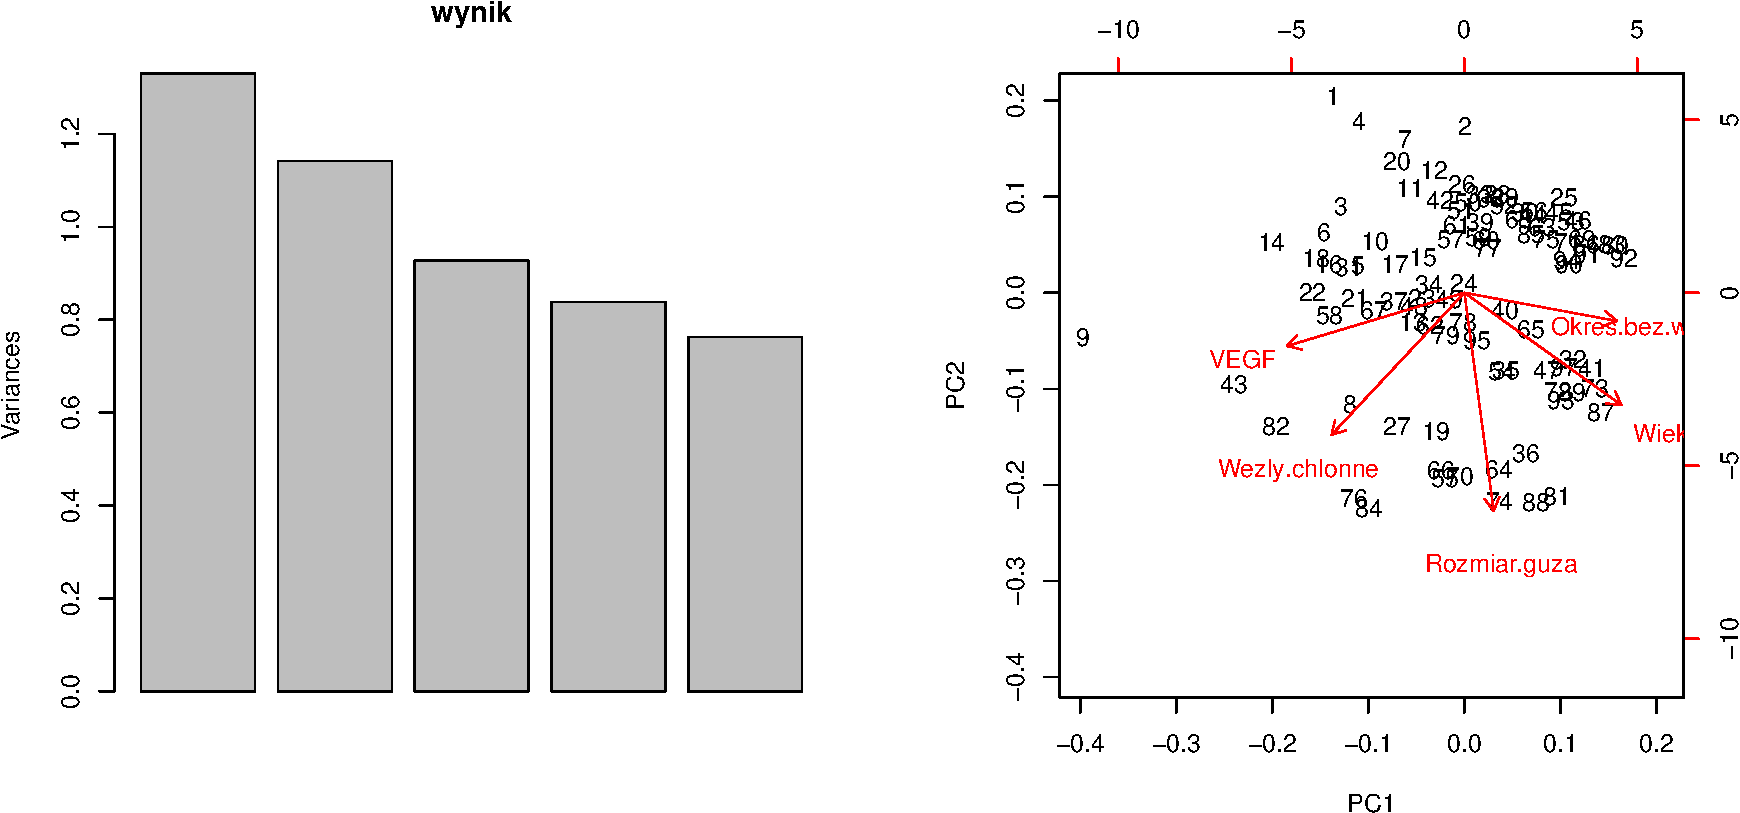
\includegraphics[width=0.7\linewidth]{NaPrzelajR_files/figure-latex/wy212-1} 

}

\caption{Graficzna reprezenacja wyników funkcji prcomp().}\label{fig:wy212}
\end{figure}

I jeszcze przykład dla danych GUSowskich

\begin{Shaded}
\begin{Highlighting}[]
\NormalTok{daneGUS <-}\StringTok{ }\KeywordTok{read.table}\NormalTok{(}\StringTok{"http://www.biecek.pl/R/dane/Dane2007GUS.csv"}\NormalTok{, }\DataTypeTok{sep=}\StringTok{";"}\NormalTok{, }\DataTypeTok{h=}\NormalTok{T, }\DataTypeTok{dec=}\StringTok{","}\NormalTok{)}
\CommentTok{# przygotowujemy dane, wybieramy tylko kolumny dotyczące studentów}
\NormalTok{dane =}\StringTok{ }\NormalTok{daneGUS[,}\DecValTok{5}\OperatorTok{:}\DecValTok{19}\NormalTok{]}
\CommentTok{# wykonujemy analizę składowych głównych}
\NormalTok{wynik =}\StringTok{ }\KeywordTok{prcomp}\NormalTok{(dane, }\DataTypeTok{scale=}\NormalTok{T)}
\CommentTok{# zamiast obrazka możemy tę informację mieć przedstawioną jako ramkę danych}
\KeywordTok{summary}\NormalTok{(wynik)}
\end{Highlighting}
\end{Shaded}

\begin{verbatim}
## Importance of components:
##                           PC1     PC2     PC3     PC4    PC5     PC6
## Standard deviation     3.3274 1.19941 0.84435 0.74182 0.5666 0.50895
## Proportion of Variance 0.7381 0.09591 0.04753 0.03669 0.0214 0.01727
## Cumulative Proportion  0.7381 0.83400 0.88153 0.91821 0.9396 0.95688
##                            PC7     PC8     PC9    PC10    PC11    PC12
## Standard deviation     0.45921 0.42930 0.36576 0.25868 0.16275 0.11174
## Proportion of Variance 0.01406 0.01229 0.00892 0.00446 0.00177 0.00083
## Cumulative Proportion  0.97094 0.98323 0.99215 0.99661 0.99837 0.99920
##                           PC13    PC14     PC15
## Standard deviation     0.09009 0.06113 0.008919
## Proportion of Variance 0.00054 0.00025 0.000010
## Cumulative Proportion  0.99975 0.99999 1.000000
\end{verbatim}

\begin{Shaded}
\begin{Highlighting}[]
\KeywordTok{par}\NormalTok{(}\DataTypeTok{mfcol=}\KeywordTok{c}\NormalTok{(}\DecValTok{1}\NormalTok{,}\DecValTok{2}\NormalTok{))}
\CommentTok{# ten wykres przedstawia ile wariancji jest wyjaśnione przez kolejne zmienne}
\KeywordTok{plot}\NormalTok{(wynik)}
\CommentTok{# narysujmy biplot dla tych wyników}
\KeywordTok{biplot}\NormalTok{(wynik)}
\end{Highlighting}
\end{Shaded}

\begin{figure}[h]

{\centering 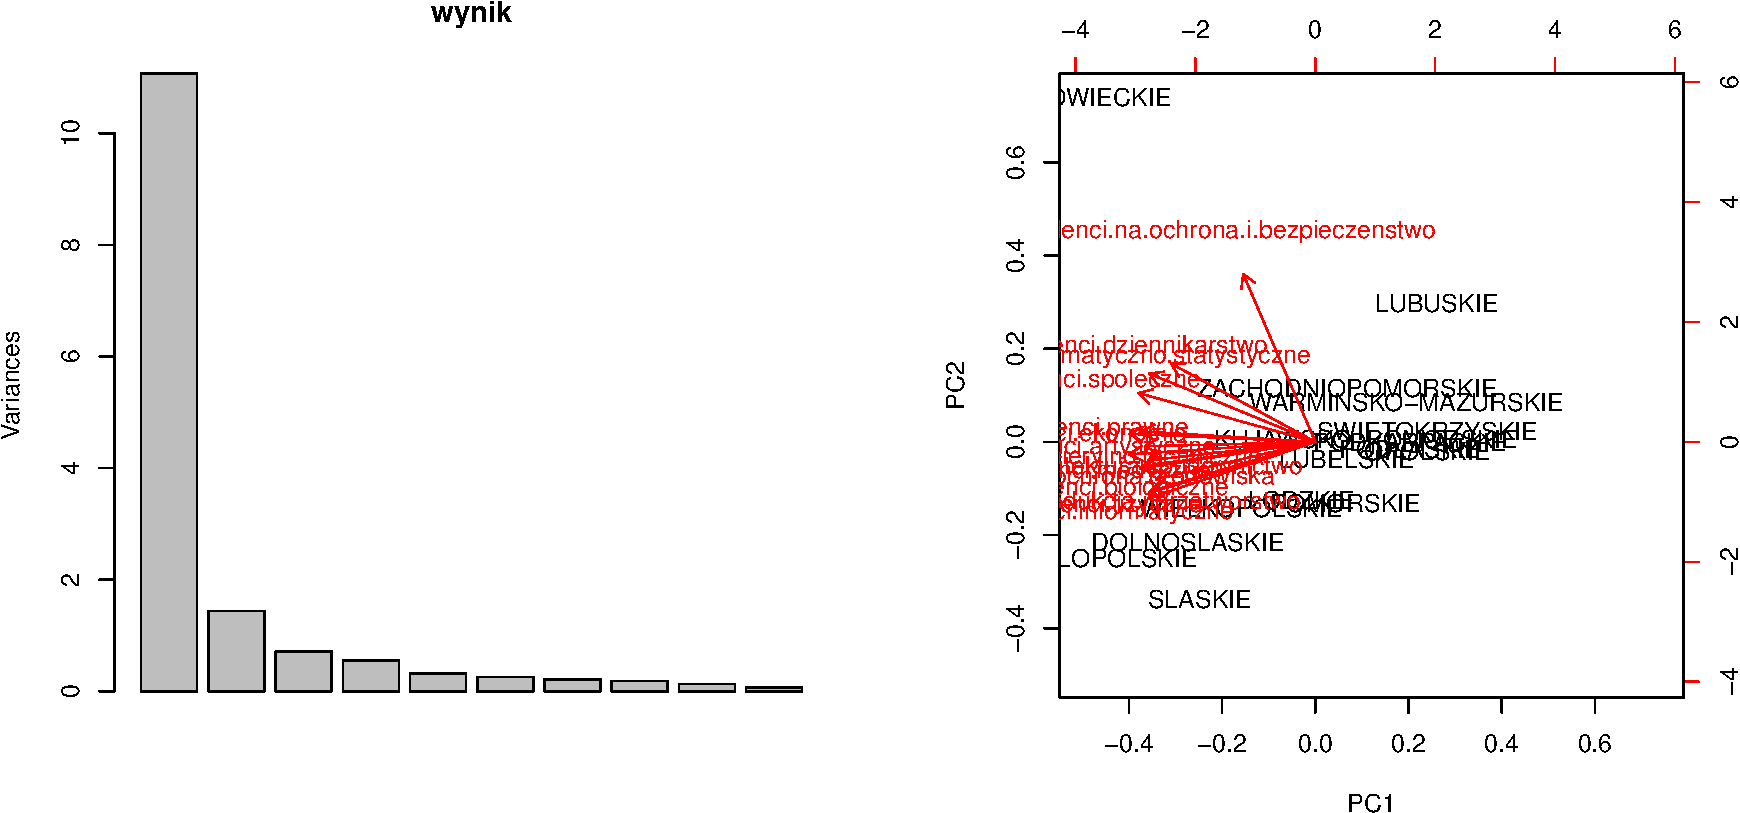
\includegraphics[width=0.7\linewidth]{NaPrzelajR_files/figure-latex/wy213-1} 

}

\caption{Graficzna reprezenacja wyników PCA dla danych GUSowych.}\label{fig:wy213}
\end{figure}

Zobaczmy jak wygląda macierz przekształcenia. Można z niej odczytać w jaki
sposób poszczególne współrzędne wpływają na kolejne składowe.

W przypadku pierwszej składowej współczynniki przy praktycznie każdej zmiennej wynoszą około \(-0,25\). W przybliżeniu oznacza to, że pierwsza składowa będzie
odpowiadała -łącznej liczbie studentów w danym województwie. A więc im więcej
studentów tym mniejsza wartość pierwszej składowej.

Druga składowa jest już ciekawsza, ponieważ różnym województwom odpowiadają różne współczynniki. Województwa o dużych wartościach na drugiej składowej
to województwa z ``nadreprezentacją'' studentów z kierunków społecznych, dziennikarstwa, matematyki i ochrony a ``niedomiarze'' studentów z nauk biologicznych, fizycznych, informatycznych i produkcji.

\begin{Shaded}
\begin{Highlighting}[]
\CommentTok{# macierz przekształcenia}
\NormalTok{wynik}\OperatorTok{$}\NormalTok{rotation[,}\DecValTok{1}\OperatorTok{:}\DecValTok{4}\NormalTok{]}
\end{Highlighting}
\end{Shaded}

\begin{verbatim}
##                                             PC1         PC2         PC3
## studenci.artystyczne                 -0.2668431 -0.01935350 -0.39012931
## studenci.spoleczne                   -0.2769475  0.21209089 -0.06445972
## studenci.ekonomia                    -0.2908474  0.03508728 -0.12031553
## studenci.prawne                      -0.2724967  0.04551798 -0.11257234
## studenci.dziennikarstwo              -0.2258601  0.34018454  0.43605864
## studenci.biologiczne                 -0.2496580 -0.16285221  0.32214165
## studenci.fizyczne                    -0.2604590 -0.22242474 -0.24023057
## studenci.matematyczno.statystyczne   -0.2599768  0.29657185  0.03841079
## studenci.informatyczne               -0.2621867 -0.24703158 -0.01225057
## studenci.medyczne                    -0.2654754 -0.10490797 -0.44763987
## studenci.inzynieryjno.techniczne     -0.2913698 -0.05414636  0.02117248
## studenci.produkcja.i.przetworstwo    -0.2521053 -0.20996741  0.24515891
## studenci.architektura.i.budownictwo  -0.2621286 -0.08025265  0.42188743
## studenci.na.ochrona.srodowiska       -0.2744594 -0.11530401  0.07394037
## studenci.na.ochrona.i.bezpieczenstwo -0.1129936  0.72998765 -0.13728919
##                                              PC4
## studenci.artystyczne                  0.06339131
## studenci.spoleczne                   -0.18107667
## studenci.ekonomia                     0.01692755
## studenci.prawne                       0.27527826
## studenci.dziennikarstwo               0.37212854
## studenci.biologiczne                  0.40296643
## studenci.fizyczne                     0.28846603
## studenci.matematyczno.statystyczne    0.13851583
## studenci.informatyczne               -0.33688023
## studenci.medyczne                     0.09636022
## studenci.inzynieryjno.techniczne     -0.08996322
## studenci.produkcja.i.przetworstwo    -0.39126146
## studenci.architektura.i.budownictwo  -0.15234913
## studenci.na.ochrona.srodowiska       -0.29601767
## studenci.na.ochrona.i.bezpieczenstwo -0.29845944
\end{verbatim}

\hypertarget{part_22}{%
\section{Nieliniowe skalowanie wielowymiarowe (Sammon Mapping)}\label{part_22}}

W przypadku metody PCA nowe współrzędne konstruowano tak, by były one kombinacjami liniowymi oryginalnych danych. To oczywiście nie jest jedyna możliwość konstrukcji nowych zmiennych. Postawmy zagadnienie skalowania następująco.

Dane: mamy \(n\) obiektów oraz macierz odległości pomiędzy każdą parą obiektów.
Oznaczmy przez \(d_ij\) odległość pomiędzy obiektem \(i\)-tym i \(j\)-tym.
Szukane: reprezentacja obiektów w przestrzeni \(k\) wymiarowej, tak by zminimalizować
\[
stress=\frac{\sum_{ij}(d_{ij}-\bar{d}_{ij})^2/d_{ij}}{\sum_{ij}d_{ij}}
\]
gdzie \(\tilde{d}_{ij}\) to odległość pomiędzy obiektami \(i\) i \(j\) w nowej \(k\)-wymiarowej przestrzeni.

Innymi słowy, szukamy (niekoniecznie liniowego) przekształcenia, które możliwie
najwierniej (w sensie ważonego błędu kwadratowego) zachowa odległości pomiędzy
obiektami. Takie przekształcenie poszukiwane jest iteracyjnie.

Jak to zrobić w R? Można np. używając funkcji \texttt{sammon(MASS)}. Pierwszym argumentem tej funkcji powinna być macierz odległości pomiędzy obiektami (np. wynik
funkcji \texttt{dist()}) a argument \texttt{k} określa na iluwymiarową przestrzeń chcemy skalować dane (domyślnie \(k = 2\)).

\begin{Shaded}
\begin{Highlighting}[]
\CommentTok{# wyznaczamy macierz odległości}
\NormalTok{odleglosci =}\StringTok{ }\KeywordTok{dist}\NormalTok{(dane)}
\CommentTok{# wyznaczamy nowe współrzędne w przestrzeni dwuwymiarowej}
\NormalTok{noweSammon =}\StringTok{ }\NormalTok{MASS}\OperatorTok{::}\KeywordTok{sammon}\NormalTok{(odleglosci, }\DataTypeTok{k=}\DecValTok{2}\NormalTok{, }\DataTypeTok{trace=}\OtherTok{FALSE}\NormalTok{)}
\CommentTok{# jak wyglądają nowe współrzędne}
\KeywordTok{head}\NormalTok{(noweSammon}\OperatorTok{$}\NormalTok{points)}
\end{Highlighting}
\end{Shaded}

\begin{verbatim}
##                          [,1]      [,2]
## DOLNOSLASKIE        15211.180 3403.2348
## KUJAWSKO-POMORSKIE  -7063.770 3448.9048
## LODZKIE              1251.418 -916.5612
## LUBELSKIE           -4912.805 1058.6175
## LUBUSKIE           -12775.224 3090.0001
## MALOPOLSKIE         21526.869 1963.5498
\end{verbatim}

\begin{table}[t]

\caption{\label{tab:tab22}Pola obiektu będącego wynikiem funkcji sammon().}
\centering
\begin{tabular}{>{}l||>{\raggedright\arraybackslash}p{35em}}
\hline
. & opis\\
\hline
$\texttt{\$points}$ & Macierz współrzędnych obiektów w nowej $k$-wymiarowej przestrzeni.\\
\hline
$\texttt{\$stress}$ & Uzyskana wartość optymalizowanego parametru stresu.\\
\hline
\end{tabular}
\end{table}

\hypertarget{part_23}{%
\section{Skalowanie wielowymiarowe Kruskalla (MDS, ang. Multidimensional Scaling)}\label{part_23}}

Jak już wspominaliśmy, metody redukcji wymiaru są często wykorzystywane do wizualizacji danych. W przypadku analizy składowych głównych po znalezieniu współrzędnych obiektów w nowej bazie wystarczy wziąć dwie pierwsze współrzędne by móc przedstawiać zbiór obserwacji na wykresie dwuwymiarowym, trzy pierwsze by móc
przedstawić zbiór obserwacji na wykresie trójwymiarowym itp. Wadą analizy składowych głównych jest uwzględnianie wyłącznie zmiennych ilościowych. Kolejnym
minusem jest konieczność posiadania wartości pomiarów dla kolejnych zmiennych,
nie można tej metody użyć w sytuacji gdy mamy wyłącznie informacje o podobieństwie lub odległości pomiędzy obiektami.

Metody skalowania Sammona i Kruskala nie mają tych wad. Są to metody ekstrakcji cech, na podstawie macierzy odległości lub macierzy niepodobieństwa pomiędzy obiektami. Celem tych metod jest wyznaczenie współrzędnych w nowym
układzie współrzędnych, w taki sposób by odległości pomiędzy obiektami w nowym
układzie współrzędnych były podobne do oryginalnych odległości pomiędzy obiektami. Przykład skalowania wielowymiarowego przedstawiliśmy na rysunku 2.4.

W przypadku skalowania Kruskala minimalizowana jest wartość
\[
stress=\frac{\sum_{ij}(f(d_{ij})-\tilde{d}_{ij})^2}{\sum_{ij}f(d_{ij})^2},
\]
gdzie \(\tilde{d}_{ij}\) to odległość pomiędzy obiektami \(i\) i \(j\) w nowej \(k\)-wymiarowej przestrzeni a d ij to oryginalne odległości pomiędzy obiektami przekształcone przez pewną monotoniczną funkcję \(f()\) (więc \(d_{ij}\) i \(\tilde{d}_{ij}\) mogą być w różnych skalach!).

\begin{figure}

{\centering \includegraphics[width=1\linewidth]{isoMDSprzykald} 

}

\caption{Przykład skalowania wielowymiarowego.}\label{fig:MDS}
\end{figure}

Skalowanie wielowymiarowe jest w R dostępne w kilku funkcjach:

\begin{itemize}
\item
  funkcja \texttt{isoMDS(MASS)} wyznacza niemetryczne skalowanie Kruskala,
\item
  funkcja \texttt{sammon(MASS)} wyznacza niemetryczne skalowanie Sammona (patrz
  poprzedni podrozdział {[}TODO: uspójnić!!{]}),
\item
  funkcja \texttt{cmdscale(stats)} wyznacza skalowanie metryczne inaczej PCA (patrz
  poprzedni podrozdział {[}TODO: uspójnić!!{]}).
\end{itemize}

Poniżej przedstawimy przykłady użycia dla funkcji isoMDS(), z pozostałych korzysta
się podobnie. Najważniejszym argumentem wejściowym do algorytmu skalowania wielowymiarowego jest macierz odległości pomiędzy obserwacjami. Wyznaczyć ją można np. funkcją \texttt{dist(stats)}. W funkcji \texttt{dist()} zaimplementowane są wszystkie
popularne metody liczenia odległości pomiędzy obserwacjami, w tym odległość euklidesowa (najpopularniejsza, odpowiadająca sumie kwadratów różnic poszczególnych współrzędnych, tej odległości odpowiada argument \texttt{method="euclidean"}), odległość Manhattan, nazywana też odległością taksówkową lub miejską (suma modułów różnic pomiędzy współrzędnymi, argument \texttt{method="manhattan"}), odległość Mińkowskiego (argument \texttt{method="minkowski"})
oraz kilka innych mniej popularnych odległości. Jeżeli w zbiorze danych znajdują się
zmienne jakościowe to funkcja \texttt{dist()} sobie z nimi nie poradzi. W takiej sytuacji
lepiej wykorzystać funkcję daisy(cluster) wyznaczającą macierz niepodobieństwa
pomiędzy obiektami. Funkcja \texttt{daisy()} uwzględnia również zmienne jakościowe (poniżej przedstawiamy przykład użycia). Macierz odległości jest obiektem klasy \texttt{dist()}
i nie jest pamiętana jako macierz, a jedynie jako połowa macierzy (ponieważ odległość jest symetryczna szkoda pamięci na przechowywanie nadmiarowych danych).
Jeżeli potrzebujemy przekształcić obiekt \texttt{dist()} na macierz to możemy wykorzystać
funkcję \texttt{as.matrix()}

Wynikiem algorytmu skalowania wielowymiarowego są współrzędne obserwacji
w pewnym nowym układzie współrzędnych. Możemy wybrać wymiar przestrzeni na
jaką mają być przeskalowane dane (argument \texttt{k} funkcji \texttt{isoMDS}). Z pewnością po wykonaniu skalowania interesować nas będzie na ile skalowanie zachowało odległości pomiędzy obiektami, czy dużo jest znacznych zniekształceń. Do oceny wyników skalowania wykorzystać można wykres Sheparda przedstawiający na jednej osi oryginalne
odległości pomiędzy obiektami a na drugiej osi odległości w nowym układzie współ
rzędnych. Do wyznaczenia obu wektorów odległości służy funkcja \texttt{Shepard(MASS)},
można też skorzystać z wrappera na tę funkcję, czyli z funkcji \texttt{stressplot(vegan)}.

Poniżej przedstawiamy przykład skalowania wielowymiarowego. Wykorzystamy
tę metodę do przedstawienia za pomocą dwuwymiarowego wykresu podobieństw
pomiędzy pacjentkami ze zbioru danych \texttt{daneO}. Graficzny wynik tych analiz jest
przedstawiony na rysunku \ref{fig:wy214}. Lewy rysunek przedstawia pacjentki w nowym dwuwymiarowym układzie współrzędnych, w tym przypadku pacjentki przedstawiane są
jako punkty. Wypełniony punkt oznacza dla niepowodzenie leczenia a więc wznowę,
a pusty w środku w oznacza wyleczenie pozytywne (widzimy, że pacjentki z niepo-
wodzeniami grupują się blisko siebie). Ciekawym było by naniesienie na ten wykres
nazwisk pacjentek i porównanie, które pacjentki pod względem zmierzonych wartości
były do siebie podobne. Prawy rysunek przedstawia dokładność skalowania, a więc
jak oryginalne odległości mają się do odległości w nowym układzie współrzędnych.

\begin{Shaded}
\begin{Highlighting}[]
\NormalTok{dane0 <-}\StringTok{ }\KeywordTok{read.table}\NormalTok{(}\StringTok{"http://www.biecek.pl/R/dane/dane0.csv"}\NormalTok{,}\DataTypeTok{sep=}\StringTok{";"}\NormalTok{,}\DataTypeTok{header =} \OtherTok{TRUE}\NormalTok{)}
\CommentTok{# konstruujemy macierz niepodobieństwa pomiędzy pacjentkami, również zmienne jakościowe są uwzględnione}
\NormalTok{niepodobienstwa =}\StringTok{ }\NormalTok{cluster}\OperatorTok{::}\KeywordTok{daisy}\NormalTok{(daneO)}
\end{Highlighting}
\end{Shaded}

\begin{verbatim}
## Warning in cluster::daisy(daneO): binary variable(s) 2, 3 treated as
## interval scaled
\end{verbatim}

\begin{Shaded}
\begin{Highlighting}[]
\CommentTok{# przeprowadzamy skalowanie niemetryczne, skalujemy do przestrzeni o}
\CommentTok{# dwóch wymiarach}
\NormalTok{skalowanie =}\StringTok{ }\NormalTok{MASS}\OperatorTok{::}\KeywordTok{isoMDS}\NormalTok{(niepodobienstwa, }\DataTypeTok{k=}\DecValTok{2}\NormalTok{)}
\end{Highlighting}
\end{Shaded}

\begin{verbatim}
## initial  value 30.138174 
## iter   5 value 25.846808
## final  value 25.531983 
## converged
\end{verbatim}

\begin{Shaded}
\begin{Highlighting}[]
\CommentTok{# obiekt wynikowy zawiera współrzędne obserwacji w~nowym układzie współrzędnych}
\KeywordTok{str}\NormalTok{(skalowanie)}
\end{Highlighting}
\end{Shaded}

\begin{verbatim}
## List of 2
##  $ points: num [1:97, 1:2] 0.1011 0.3147 -0.1055 0.2811 -0.0604 ...
##   ..- attr(*, "dimnames")=List of 2
##   .. ..$ : chr [1:97] "1" "2" "3" "4" ...
##   .. ..$ : NULL
##  $ stress: num 25.5
\end{verbatim}

\begin{Shaded}
\begin{Highlighting}[]
\CommentTok{# konstruujemy wektor pomocniczy do rysowania}
\NormalTok{ksztalty =}\StringTok{ }\KeywordTok{ifelse}\NormalTok{(daneO}\OperatorTok{$}\NormalTok{Niepowodzenia}\OperatorTok{==}\StringTok{"brak"}\NormalTok{, }\DecValTok{21}\NormalTok{, }\DecValTok{19}\NormalTok{)}
\end{Highlighting}
\end{Shaded}

\begin{Shaded}
\begin{Highlighting}[]
\KeywordTok{par}\NormalTok{(}\DataTypeTok{mfcol=}\KeywordTok{c}\NormalTok{(}\DecValTok{1}\NormalTok{,}\DecValTok{2}\NormalTok{))}
\CommentTok{# rysujemy pacjentki w~nowym układzie współrzędnych}
\KeywordTok{plot}\NormalTok{(skalowanie}\OperatorTok{$}\NormalTok{points, }\DataTypeTok{type =} \StringTok{"p"}\NormalTok{, }\DataTypeTok{pch=}\NormalTok{ksztalty, }\DataTypeTok{cex=}\FloatTok{1.5}\NormalTok{)}
\CommentTok{# rysujemy również diagram Sheparda}
\NormalTok{shepard <-}\StringTok{ }\NormalTok{MASS}\OperatorTok{::}\KeywordTok{Shepard}\NormalTok{(niepodobienstwa, skalowanie}\OperatorTok{$}\NormalTok{points)}
\KeywordTok{plot}\NormalTok{(shepard, }\DataTypeTok{pch =} \StringTok{"."}\NormalTok{)}
\KeywordTok{abline}\NormalTok{(}\DecValTok{0}\NormalTok{,}\DecValTok{1}\NormalTok{)}
\end{Highlighting}
\end{Shaded}

\begin{figure}[h]

{\centering 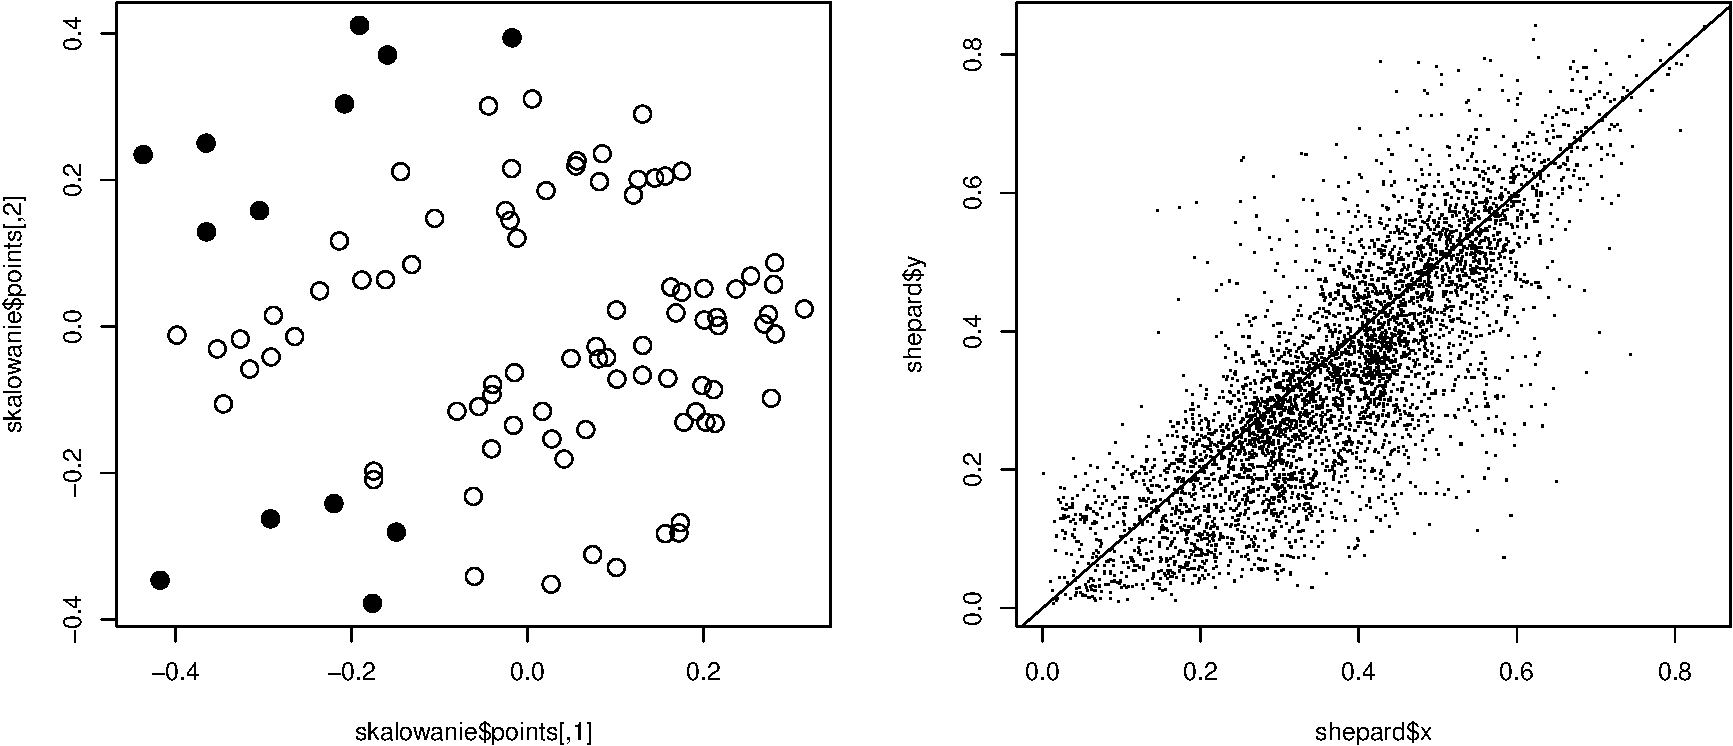
\includegraphics[width=0.7\linewidth]{NaPrzelajR_files/figure-latex/wy214-1} 

}

\caption{Graficzna reprezentacja wyników funkcji isoMDS() i Shepard().}\label{fig:wy214}
\end{figure}

Zobaczmy jak wyglądają dane o województwach po przeskalowaniu różnymi metodami. Na wykresie \ref{fig:skal3} po lewej stronie przedstawiamy przeskalowane dane a po
prawej wykresy Sheparda.

\begin{figure}

{\centering \includegraphics[width=0.85\linewidth]{skalowanie3} 

}

\caption{Graficzna reprezentacja wyników różnych funkcji skalowania, na przykładach danych GUS.}\label{fig:skal3}
\end{figure}

\hypertarget{part_3}{%
\chapter{Analiza skupień}\label{part_3}}

Analiza skupień to zbiór metod pozwalających na wyróżnienie zbiorów obserwacji
(nazywanych skupieniami lub klastrami) podobnych do siebie. Proces szukania podziału na grupy, nazywany jest czasem klastrowaniem. W pakiecie R dostępnych
jest bardzo wiele metod do przeprowadzania analizy skupień. Poniżej omówimy jedynie kilka wybranych funkcji z pakietów \texttt{cluster} i \texttt{stats}. Osoby zainteresowane
tym tematem powinny przyjrzeć się również funkcjom z pakietów \texttt{flexclust} oraz
\texttt{mclust02}.

Wyniki działania wybranych procedur analizy skupień przedstawimy ma przykładzie zbioru danych benchmarkowych. W pakiecie mlbench (skrót od Machine
Learning Benchmark Problems) umieszczonych jest wiele ciekawych zbiorów danych
wykorzystywanych do testowania właściwości algorytmów dyskryminacji lub analizy skupień. W tym pakiecie znajdują się zbiory rzeczywistych danych, jak również
funkcje do generowania zbiorów danych o określonych kształtach lub właściwościach.
Dwa zbiory wygenerowanych danych na których będziemy testować metody analizy skupień przedstawione są na rysunku \ref{fig:mlbench}. Zostały one wygenerowane funkcjami
\texttt{mlbench.cassini(mlbench)} i \texttt{mlbench.2dnormals(mlbench)}.

Do wyznaczania skupisk wystarczy macierz odległości pomiędzy obiektami. Domyślnie wyznaczane są odległości euklidesowe (może więc warto skalować dane?)
ale można te odległości liczyć korzystając z innych funkcji \texttt{dist.BC(clusterSim)},
\texttt{dist.GDM(clusterSim)}, \texttt{dist.SM(clusterSim)}, \texttt{dist(stats)}, \texttt{dist.binary(ade4)}.

\hypertarget{part_31}{%
\section{Metoda k-średnich}\label{part_31}}

Celem tej metody jest podział zbioru danych na \texttt{k} klastrów. Dobry podział to taki,
w którym suma odległości obserwacji należących do klastra jest znacznie mniejsza
od sumie odległości obserwacji pomiędzy klastrami. Metoda k-średnich polega na
wyznaczeniu współrzędnych \texttt{k} punktów, które zostaną uznane za środki klastrów.
Obserwacja będzie należała do tego klastra, którego środek jest najbliżej niej.

Metoda k-średnich jest zaimplementowana w funkcji \texttt{kmeans(stats)}. Pierwszym
argumentem tej funkcji jest ramka danych określająca wartości zmiennych dla kolejnych obserwacji. Drugim argumentem może być pojedyncza liczba określająca ile
klastrów chcemy identyfikować (w tym przypadku środki klastrów będą wyznaczone
iteracyjnym algorytmem) lub wektor środków klastrów. Algorytm wyboru środków
klastrów jest algorytmem zrandomizowanym, może też dawać różne wyniki nawet
na tym samym zbiorze danych! Dlatego też zalecane jest uruchomienie kilkukrotne
tego algorytmu oraz wybranie najlepsze go podziału na klastry. Można to zrobić też
automatycznie, określając argument \texttt{nstart} funkcji \texttt{kmeans()}.

Algorytm k-średnich minimalizuje \(tr(W)\) gdzie \(W\) to macierz kowariancji wewnątrz klas. Opisuje go poniższa sekwencja

\begin{enumerate}
\def\labelenumi{\arabic{enumi}.}
\item
  wybierany jest wstępny podział (w razie potrzeby można ten wybór powtórzyć
  wielokrotnie by znaleźć globalne maksimum),
\item
  przypisuje się obiekty do klasy z najbliższym środkiem ciężkości
\item
  przelicza się środki ciężkości dla nowych klas
\item
  kroki 2-3 powtarza się tak długo aż nie będą zachodziły żadne zmiany.
\end{enumerate}

\begin{figure}[h]

{\centering \includegraphics[width=1\linewidth]{mlbench} 

}

\caption{Dane, na których będziemy przedstawiać metody analizy skupień.}\label{fig:mlbench}
\end{figure}

Poniżej prezentujemy przykład użycia funkcji \texttt{kmeans()}. Wyniki analizy skupień
przedstawione są graficznie na rysunku \ref{fig:kmeans}. Różne klastry zaznaczono punktami
o różnych kształtach. Czarne pełne punkty wskazują na środki znalezionych klastrów. Oczywiście właściwszym byłoby dopasowanie do lewego przykładu 3 klastrów, a do prawego 5 klastrów. Na przedstawionych przykładach możemy prześledzić ci się dzieje, jeżeli źle określimy liczbę klastrów (czytelnik powinien spróbować powtórzyć te analizy, wyniki najprawdopodobniej otrzyma inne!).

\begin{verbatim}
# szukamy 5 klastrow, nie trafiło się nam najlepsze dopasowanie
> klaster = kmeans(zbiorPerla,5)
# jak wygląda wynik w środku?
# pole $cluster określa numer klastra dla kolejnych punktów, $centers
# określa współrzędne środków klastrów
> str(klaster)
List of 4
$ cluster : int [1:1000] 3 3 3 3 3 3 3 3 3 3 ...
$ centers : num [1:5, 1:2] 0.03203 -0.00749 -0.08380 -0.81601 0.91808
...
..- attr(*, "dimnames")=List of 2
.. ..$ : chr [1:5] "1" "2" "3" "4" ...
.. ..$ : NULL
$ withinss: num [1:5] 22.4 10.9 126.9 11.5
9.8
$ size
: int [1:5] 103 69 197 70 61
- attr(*, "class")= chr "kmeans"
# rysujemy punkty, różne klastry oznaczamy innymi kształtami punktów
> plot(zbiorPerla, pch=klaster$cluster)
# dorysujmy środki klastrów
> points(klaster$centers, cex=2, pch=19)
> klaster = kmeans(zbiorGwiazda,2)
> plot(zbiorGwiazda, pch=klaster$cluster)
> points(klaster$centers, cex=2, pch=19)
\end{verbatim}

Na powyższym przykładzie przedstawiliśmy pola w obiektach przekazanych przez
funkcję \texttt{kmeans()}. Pole \texttt{\$cluster} określa do jakiego klastra została przyporządkowana dana obserwacja, a pole \texttt{\$centers} to współrzędne środków poszczególnych klastrów.

\begin{figure}

{\centering \includegraphics[width=1\linewidth]{kmeans} 

}

\caption{Graficzna prezentacja działania funkcji kmeans().}\label{fig:kmeans}
\end{figure}

\hypertarget{part_32}{%
\section{Metoda grupowania wokół centroidów (PAM, ang. Partitioning Around Medoids)}\label{part_32}}

Metoda PAM działa na podobnej zasadzie jak k-średnich, z tą różnicą, że środkami klastrów są obserwacje ze zbioru danych (nazywane centroidami lub centrami
klastrów). W metodzie PAM zbiór możliwych środków klastrów jest więc znacznie
mniejszy, niż w metodzie k-średnich, zazwyczaj też wyniki działania metody PAM
są stabilniejsze. Na rysunku \ref{fig:pam} przedstawiony jest wynik działania poniższego przykładowego wywołania tej funkcji. Podobnie jak poprzednio różne klastry zaznaczono
punktami o różnych kształtach. Czarne pełne punkty to środki klastrów (w tej metodzie odpowiadają przypadkom ze zbioru danych).

\begin{verbatim}
# ponownie szukamy 5 klastrow
> klaster = pam(zbiorPerla,5)
> # jak wygląda wynik w środku?
  # pole $medoids określa współrzędne środków klastrów (wybranych
  # przypadków), $in.med określa indeksy obserwacji, które są środkami
  # klastrów, $clustering to wektor indeksów kolejnych klastrów, $silinfo
  # to informacje o dopasowaniu danego obiektu do klastra w którym się
  # znajduje (wartość silhouette)
> str(klaster)
List of 10
$ medoids
: num [1:5, 1:2] 6.47e-01 -6.26e-01 -6.38e-01 5.87e-01
1.59e-05 ...
$ id.med
: int [1:5] 24 126 230 267 464
$ clustering: int [1:1000] 1 1 2 1 1 2 1 1 1 2 ...
$ objective : Named num [1:2] 0.526 0.461
..- attr(*, "names")= chr [1:2] "build" "swap"
$ isolation : Factor w/ 3 levels "no","L","L*": 1 1 1 1 1
..- attr(*, "names")= chr [1:5] "1" "2" "3" "4" ...
$ clusinfo : num [1:5, 1:5] 87 113 101 99 100 ...
..- attr(*, "dimnames")=List of 2
.. ..$ : NULL
.. ..$ : chr [1:5] "size" "max_diss" "av_diss" "diameter" ...
$ silinfo
:List of 3
..$ widths
: num [1:1000, 1:3] 1 1 1 1 1 1 1 1 1 1 ...
.. ..- attr(*, "dimnames")=List of 2
.. .. ..$ : chr [1:500] "12" "96" "133" "155" ...
.. .. ..$ : chr [1:3] "cluster" "neighbor" "sil_width"
..$ clus.avg.widths: num [1:5] 0.434 0.440 0.482 0.443 0.508
..$ avg.width
: num 0.462
$ diss
: NULL
$ call
: language pam(x = zb1$x, k = 5)
$ data
: num [1:1000, 1:2] 0.0964 0.6938 -0.5325 1.2839 0.1743
...
- attr(*, "class")= chr [1:2] "pam" "partition"
> # rysujemy punkty, różne klastry oznaczamy innymi kształtami punktów
> plot(zbiorPerla, pch=klaster$clustering)
> # dorysujmy środki klastrów
> points(klaster$meoids, cex=2, pch=19)
\end{verbatim}

Obiekt, będący wynikiem funkcji \texttt{pam()} ma sporo pól, najistotniejsze to \texttt{\$medoids}
ze współrzędnymi medoidów, \texttt{\$id.med} z indeksami medoidów i \texttt{\$clustering} z indeksami klastrów, do których zostały przypisane kolejne obserwacje.

\begin{figure}[h]

{\centering \includegraphics[width=1\linewidth]{pam} 

}

\caption{Graficzna prezentacja działania funkcji pam().}\label{fig:pam}
\end{figure}

Metoda PAM jest obliczeniowo złożona. Może być niemożliwym obliczeniowo
wykonanie jej na dużym zbiorze danych. Do klastrowania dużych zbiorów polecana jest metoda clara (Clustering Large Applications) zaimplementowana w funkcji
\texttt{clara(cluster)}. Wykonuje ona wielokrotnie metodę PAM na mniejszych zbiorach
danych i scala wyniki w jeden podział na klastry.

Algorytm PAM (k-medoidów) opisuje następująca sekwencja

\begin{enumerate}
\def\labelenumi{\arabic{enumi}.}
\item
  wybiera się początkowy zbiór medoidów,
\item
  przepisuje się obiekty do klas o najbliższym medoidzie,
\item
  zmienia się medoidy o ile jest taka potrzeba, w takiej sytuacji wraca się do
  kroku 2.
\end{enumerate}

Minimalizowana jest \(\sum_{r=1}^{u}d(r)\), gdzie \(d(r)\) to najmniejsza z sum odległości jednego punktu z klasy \(r\) do wszystkich pozostałych punktów z tej klasy.

\hypertarget{part_33}{%
\section{Metoda aglomeracyjnego klastrowania hierarchicznego}\label{part_33}}

Klastrowanie hierarchiczne różni się od przedstawionych powyżej metod tym, że
zamiast dzielić obserwacje na określoną liczbę klastrów, określa się stopień podobieństwa poszczególnych obiektów i wyznacza się drzewo odpowiadające tym podobieństwom. Do budowy takich drzew wykorzystywane są różne algorytmy.

Algorytm AGglomerative NESting (AGNES) jest metodą aglomeracyjną, co oznacza, że w pierwszym kroku każda obserwacja traktowana jest jak osobny klaster.
W kolejnych krokach klastry najbardziej podobne do siebie są łączone w coraz większe klastry, tak długo aż nie powstanie tylko jeden klaster. Algorytm aglomeracyjnego klastrowania hierarchicznego jest dostępny w funkcji \texttt{agnes(cluster)}. Pierwszym argumentem może być macierz danych (podobnie jak w przypadku innych algorytmów klastrowania) określająca współrzędne poszczególnych obserwacji lub też
macierz odległości pomiędzy obserwacjami, a więc obiekt klasy \texttt{dist} (jak tworzyć
takie obiekty pisaliśmy w poprzednim podrozdziale). Duże znaczenie ma metoda
liczenia odległości pomiędzy obserwacjami. Z reguły zmiana metody liczenia odległości (np. z euklidesowej na taksówkową) prowadzi do otrzymania zupełnie innego wyniku.

Algorytm grupowania hierarchicznego można opisać następująco:

\begin{enumerate}
\def\labelenumi{\arabic{enumi}.}
\item
  Każdą obserwacje traktujemy jako osobne skupienie.
\item
  Znajdujemy dwa skupiska najbliższe sobie. Odległość pomiędzy skupiskami
  można wyznaczać na różne sposoby. Trzy najpopularniejsze opisane są poniżej.
\item
  Łączymy dwa najbliższe skupiska w jedno.
\item
  Jeżeli pozostało więcej niż jedno skupisko to wracamy do kroku 2.
\end{enumerate}

Kolejnym istotnym argumentem jest argument \texttt{method}. Określa on kolejność łączenia małych klastrów w coraz większe klastry. W każdym kroku łączone są najbliższe klastry, ale odległość pomiędzy dwoma klasterami można liczyć na trzy sposoby:

\begin{itemize}
\item
  \texttt{method="single"}, liczona jest odległość pomiędzy najbliższymi punktami każdego z klastrów, do jednego klastra dołączany jest klaster którego dowolny element jest najbliżej. Ta metoda odpowiada zachłannemu dodawania do skupiska
  obiektów bliskich brzegowi skupiska, możliwe jest tworzenie się tzw. łańcuchów
  kolejno dołączanych obiektów, być może już nie tak podobnych do całego skupiska, coś w stylu „przyjaciele naszych przyjaciół są naszymi przyjaciółmi'',
\item
  \texttt{method="average"}, liczona jest średnia odległość pomiędzy punktami każdego
  z klastrów, łączone są więc klastry średnio podobnych obserwacji, to jedna z
  popularniejszych metod ({[}unweighted pair-{]}group average method, UPGMA),
\item
  \texttt{method="complete"}, liczona jest odległość pomiędzy najdalszymi punktami
  każdego z klastrów, jeżeli dwa skupiska są w odległości \(d\) oznacza to, że że
  każda para punktów w tych skupiskach jest nie bardziej odległa niż \(d\).
\item
  \texttt{method="ward"} skupiska o minimalnej wariancji, w wyniku otrzymuje się zwarte skupiska.
\item
  \texttt{method="flexible"}, elastyczność tej metody polega na możliwości określenia
  jak liczona ma być odległość pomiędzy łączonymi klastrami. Tą odległość sparametryzowano czterema współczynnikami (więcej informacji znaleźć można w \citet{KR1990}, p.237 lub w opisie funkcji \texttt{agnes()}). Korzystanie z tej opcji polecane jest
  bardziej doświadczonym użytkownikom, działa zasada: nie wiesz jak to działa
  nie używaj.
\item
  \texttt{method="weighted"} odpowiada metodzie elastyczne z parametrem \texttt{par.method\ =\ 0.5}.
\end{itemize}

\begin{quote}
\emph{Dla funkcji \texttt{agnes()} domyślnie stosowana jest metoda \texttt{average}, a dla
funkcji \texttt{hclust()} domyślnie stosowana jest \texttt{complete}. Funkcja \texttt{agnes()}
w porównaniu do innych implementacji ma dwie dodatkowe cechy: wyznacza ``agglomerative coefficient'' i umożliwia rysowanie ``banner.plot''."}
\end{quote}

Użycie każdej z tych metod prowadzi do wygenerowania innego drzewa. Wyniki
dla każdej z tych trzech wymienionych metod łączenia klastrów oraz dla obu zbiorów danych przedstawiamy na rysunku \ref{fig:agnes}. Na tym rysunku przedstawione są wyniki
analizy skupień dla 1000 obiektów, jeżeli analizujemy mniejszą liczbę obiektów, to
na osi poziomej można odczytać nazwy poszczególnych obiektów a tym samym wizualizować, które obiekty są do siebie bardziej, a które mniej podobne (przykład
takiego drzewa przedstawiliśmy na rysunku \ref{fig:hc35}).

Wracając do rysunku \ref{fig:agnes} w przypadku zbioru Gwiazda sensowniejsze wyniki
otrzymuje się dla metod łączenia \texttt{average} i \texttt{complete} (na drzewie można wydzielić
5 podgałęzi odpowiadającym spodziewanym skupiskom). Dla zbioru Perła najlepiej
radzi sobie metoda łączenia \texttt{single} wyodrębniająca dosyć szybko trzy rozłączne
skupiska. Najczęściej wykorzystywaną metodą łączenia jest \texttt{average}, nie oznacza to że zawsze daje najlepsze wyniki.

Aby na podstawie hierarchicznego klastrowania przypisać obserwacje do określonej liczby klastrów należy drzewo przyciąć na pewnej wysokości. Do przycinania
drzewa służy funkcja \texttt{cutree(stats)}, jej pierwszym argumentem jest obiekt będący
wynikiem metody hierarchicznej. Kolejnym argumentem, który należy wskazać jest
\texttt{k} (określa do ilu klastrów chcemy przyciąć drzewo) lub \texttt{h} (określa na jakiej wysokości
chcemy przyciąć drzewo). Wysokość drzewa na której chcemy odciąć klastry można
odczytać z rysunków wygenerowanych dla tego drzewa.

Poniżej przedstawiamy przykład wywołania funkcji \texttt{agnes()} i \texttt{cuttree()}.

\begin{verbatim}
# wywołanie funkcji AGNES
> klaster = agnes(zbiorPerla, method="average")
# wynik możemy narysować przeciążoną funkcją plot
> plot(klaster)
# otrzymane drzewo możęmy przyciąć do określonej liczby klastrów
> etykietkiKlastrow = cutree(klaster, k=2)
\end{verbatim}

\begin{figure}

{\centering \includegraphics[width=1\linewidth]{agnes} 

}

\caption{Graficzny przykład wyników funkcji agnes().}\label{fig:agnes}
\end{figure}

\begin{Shaded}
\begin{Highlighting}[]
\KeywordTok{library}\NormalTok{(}\StringTok{"MASS"}\NormalTok{)}
\end{Highlighting}
\end{Shaded}

\begin{verbatim}
## 
## Attaching package: 'MASS'
\end{verbatim}

\begin{verbatim}
## The following object is masked from 'package:dplyr':
## 
##     select
\end{verbatim}

\begin{Shaded}
\begin{Highlighting}[]
\KeywordTok{data}\NormalTok{(Cars93)}
\NormalTok{Cars93}\OperatorTok{$}\NormalTok{y =}\StringTok{ }\KeywordTok{sapply}\NormalTok{(}\DecValTok{1}\OperatorTok{:}\DecValTok{93}\NormalTok{,}\ControlFlowTok{function}\NormalTok{(i) }\KeywordTok{paste}\NormalTok{(Cars93[i,}\DecValTok{1}\NormalTok{],Cars93[i,}\DecValTok{2}\NormalTok{],}\DataTypeTok{sep=}\StringTok{" "}\NormalTok{))}
\NormalTok{h =}\StringTok{ }\NormalTok{Cars93[,}\KeywordTok{c}\NormalTok{(}\DecValTok{4}\NormalTok{,}\DecValTok{5}\NormalTok{,}\DecValTok{6}\NormalTok{,}\DecValTok{7}\NormalTok{,}\DecValTok{8}\NormalTok{,}\DecValTok{11}\NormalTok{,}\DecValTok{12}\NormalTok{,}\DecValTok{13}\NormalTok{,}\DecValTok{14}\NormalTok{,}\DecValTok{15}\NormalTok{,}\DecValTok{17}\NormalTok{,}\DecValTok{18}\NormalTok{,}\DecValTok{19}\NormalTok{,}\DecValTok{20}\NormalTok{,}\DecValTok{21}\NormalTok{,}\DecValTok{22}\NormalTok{,}\DecValTok{23}\NormalTok{,}\DecValTok{24}\NormalTok{,}\DecValTok{25}\NormalTok{)]}
\KeywordTok{rownames}\NormalTok{(h) =}\StringTok{ }\NormalTok{Cars93}\OperatorTok{$}\NormalTok{y}
\NormalTok{c =}\StringTok{ }\KeywordTok{hclust}\NormalTok{(}\KeywordTok{dist}\NormalTok{(h[}\DecValTok{1}\OperatorTok{:}\DecValTok{37}\NormalTok{,]))}
\KeywordTok{plot}\NormalTok{(c)}
\end{Highlighting}
\end{Shaded}

\begin{figure}[h]

{\centering 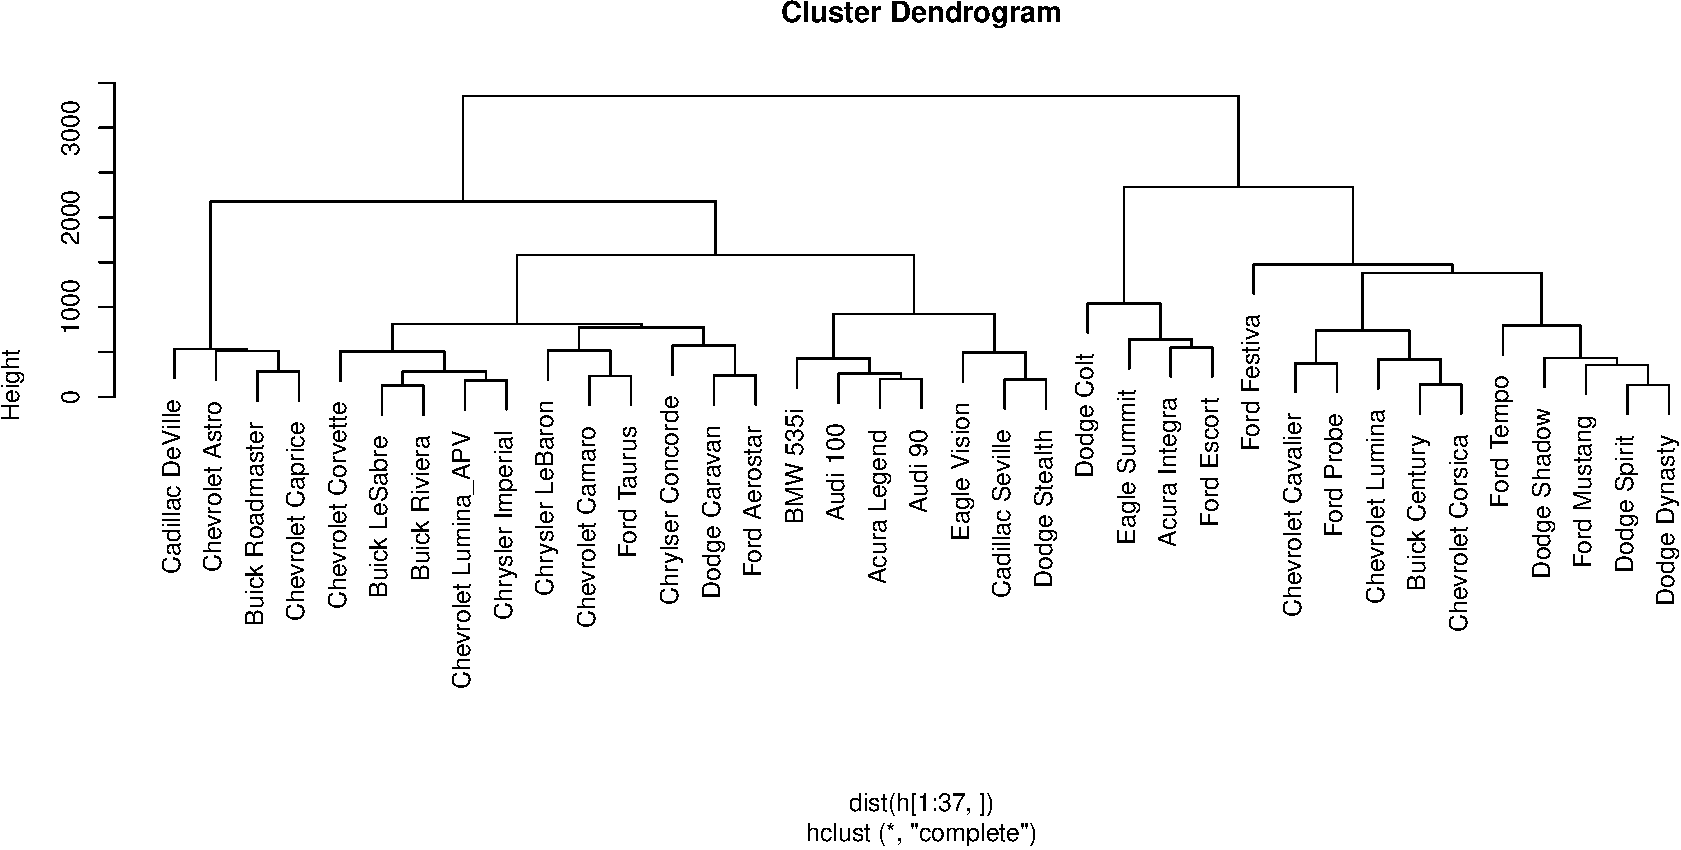
\includegraphics[width=0.7\linewidth]{NaPrzelajR_files/figure-latex/hc35-1} 

}

\caption{Drzewo dla wybranych modeli samochodów na bazie zbioru danych (Cars93(MASS)).}\label{fig:hc35}
\end{figure}

\hypertarget{part_34}{%
\section{Ile skupień wybrać?}\label{part_34}}

Krótka odpowiedź na to pytanie brzmi 5. Długa wymaga odpowiedzi na dodatkowe
pytanie, na czym nam zależy wybierając liczbę skupień? Co chcemy z tymi skupieniami robić i po co je wyznaczmy.

Popularną techniką wyboru liczby skupień jest rysowanie pewnej statystyki jako
funkcji liczby skupień i wybór takiej liczby skupień dla której dana statystyka spełnia
nasze oczekiwania (np. osiąga maksimum lub najszybciej maleje). Wiele przydatnych
statystyk opisujących jakość podziału na grupy znajduje się w pakiecie \texttt{clusterSim}.

Popularne indeksy służące do wyboru liczby klastrów to:

\begin{itemize}
\item
  \(tr(B)/tr(W)\) gdzie \(B\) to macierz kowariancji wewnątrzklasowej a \(W\) to macierz
  kowariancji miedzyklasowej,
\item
  \(B_u/(u-1)/W_u(n-u)\) czyli miara zaproponowana przez Calińskiego i Harabasza (viva Poznań),
\item
  sylwetka (silhouette) \(S(u)=1/n\sum_{i=1}^{n}(b(i)-a(i))/max(a(i),b(i))\) średnie podobieństwo obiektów do klastrów w których się znajdują, \(a(i)\) to średnia odległość pomiędzy obiektem \(i\) a pozostałymi w tym samym klastrze, \(b(i)\) to średnia odległość obiektu \(i\) od obiektów z najbliższego skupiska do \(i\) (do którego \(i\) nie należy).
\end{itemize}

Wiele indeksów wyznaczyć można korzystając z funkcji \texttt{index.G1(clusterSim)},
\texttt{index.G2(clusterSim)}, \texttt{index.G3(clusterSim)}, \texttt{index.S(clusterSim)}, \texttt{index.KL(clusterSim)},
\texttt{index.H(clusterSim)}, \texttt{index.Gap(clusterSim)}, \texttt{index.DB(clusterSim)}.

Funkcja \texttt{index.G1(clusterSim)} wyznacza indeks Calińskiego i Harabasza, funkcja \texttt{index.S(clusterSim)} wyznacza średnią sylwetkę (silhouette).

TODO: opisać funkcję \texttt{cluster.Description(clusterSim)} pozwalającą na opisywanie znalezionych klas.

\hypertarget{part_35}{%
\section{Inne metody analizy skupień}\label{part_35}}

Poza wymienionymi powyżej trzema metodami, w pakiecie R dostępnych jest wiele
innych metod do analizy skupień. Poniżej wymienimy inne popularne.

\begin{itemize}
\tightlist
\item
  \textbf{Metoda hierarchiczej analizy skupień przez dzielenie}. Metoda hierarchicznego klastrowania przez łączenie działała w ten sposób, że zaczynając
  od małych, jednopunktowych klastrów w procesie łączenia klastrów otrzymywało się hierarchiczną zależność. Metoda analizy skupień przez dzielenie
  działa w przeciwnym kierunku. Zaczynając od jednego dużego klastra, w kolejnych krokach ten klaster jest dzielony na mniejsze klastry, aż do otrzymania jednoelementowych klastrów. Ta metoda jest zaimplementowana w funkcji
  \texttt{diana(cluster)}.
\end{itemize}

Algorytm działania metody \texttt{diana()} opisany jest poniżej

\begin{enumerate}
\def\labelenumi{\arabic{enumi}.}
\item
  dla każdego skupiska wyznaczamy maksymalną odległość pomiędzy dwo-
  ma obserwacjami w skupisku,
\item
  wybieramy skupisko o największej średnicy, w tym skupisku szukamy
  obiektu o największej średniej odległości od pozostałych, to będzie zalążek nowego skupiska,
\item
  dla każdego obiektu sprawdzamy czy nie jest średnio bliżej obiektom z
  klasy nowej niż obiektom z klasy starej, w razie potrzeby zmieniana jest
  klasa
\item
  punkt 3 powtarzany jest tak długo aż nie będzie potrzeby zmieniać przynależności żadnego punktu
\end{enumerate}

\begin{itemize}
\item
  \textbf{Metoda klastrowania rozmytego}. Jeżeli w procesie klastrowania dopuszczamy rozmytą przynależność do klastra (np. obserwacja może z pewnymi
  współczynnikami przynależeć do różnych klastrów) to uzasadnionym jest użycie metody klastrowania rozmytego. Ta metoda jest zaimplementowana w funkcji \texttt{fanny(cluster)}.
\item
  \textbf{Inne metody hierarchiczego klastrowania}. Podobna w działaniu do
  \texttt{agnes()} metoda klastrowania hirarchicznego dostępna w funkcji \texttt{hclust(stats)}.
  Umożliwia ona większy wybór metody łączenia klastrów. Argumentem method
  należy wskazać jeden z wielu dostępnych indeksów do określania odległości pomiędzy klastrami, dostępne są indeksy znane z funkcji \texttt{agnes()} oraz \texttt{"mcquitty"},
  \texttt{"ward"} i \texttt{"centroid"}.
\end{itemize}

Wykonać klastrowanie jest stosunkowo prosto, jednak to jeszcze nie jest koniec
pracy, potrzebne są metody oceny jakości podziału na skupiska. Do oceny jakości
klastrowania można wykorzystać współczynnik silhouette, określający podobieństwo
obiektu do innych obiektów w tym samym klastrze. Ten indeks jest wyznaczany przez
funkcje \texttt{silhouette(cluster)}. Poniżej przedstawiamy przykład użycia tej funkcji,
a na rysunku \ref{fig:silhouette} przedstawiamy dopasowania poszczególnych punktów do klastrów.
Wiele innych metod do oceny wyników klastrowania oraz badania zgodności dwóch
podziałów na klastry jest dostępnych w pakiecie \texttt{clv}.

\begin{verbatim}
> kluster <- pam(zbiorPerla, 5)
> sil <- silhouette(kluster)
> summary(sil)
Silhouette of 1000 units in 5 clusters from pam(x = zbiorPerla, k = 5) :
Cluster sizes and average silhouette widths:
      198       202       237       163       200
0.5005513 0.4711742 0.4402300 0.5146160 0.5240964
Individual silhouette widths:
   Min. 1st Qu.  Median    Mean 3rd Qu.    Max.
-0.1238  0.3895  0.5330  0.4873 0.6111   0.7220
> plot(sil, col = c("red", "green", "blue", "purple","yellow"))
\end{verbatim}

\begin{figure}

{\centering \includegraphics[width=0.7\linewidth]{silhouette} 

}

\caption{Wykres dopasowania punktów do poszczególnych klastrów z użyciem miary silhouette.}\label{fig:silhouette}
\end{figure}
\begin{figure}

{\centering \includegraphics[width=0.7\linewidth]{silhouetteB} 

}

\caption{Wartości funkcji silhouette dla różnych liczb klastrów wyznaczonych algorytmem PAM na zbiorze danych Gwiazda.}\label{fig:silhouetteB}
\end{figure}

Miara silhouette może użyta do wyznaczeniu liczby klastrów, na które należy
podzielić dane. Na rysunku \ref{fig:silhouetteB} przedstawiono zależność pomiędzy średnim współczynnikiem silhouette a liczbą klastrów wyznaczonych algorytmem PAN dla zbioru danych Gwiazda. W tym przypadku wyraźnie najlepszym wyborem jest 5 klastrów. Niestety w rzeczywistych problemach wybór klastrów nie jest tak prosty.

\begin{Shaded}
\begin{Highlighting}[]
\CommentTok{# cztery skupiska, dla pewności inicjujemy 25 razy}
\CommentTok{#}
\NormalTok{dane =}\StringTok{ }\NormalTok{daneGUS[,}\KeywordTok{c}\NormalTok{(}\DecValTok{22}\OperatorTok{:}\DecValTok{25}\NormalTok{)]}
\NormalTok{gus.k4 =}\StringTok{ }\KeywordTok{kmeans}\NormalTok{(dane, }\DecValTok{4}\NormalTok{, }\DataTypeTok{nstart=}\DecValTok{25}\NormalTok{)}
\NormalTok{cluster}\OperatorTok{::}\KeywordTok{silhouette}\NormalTok{(gus.k4}\OperatorTok{$}\NormalTok{clust, }\KeywordTok{dist}\NormalTok{(dane))[,}\DecValTok{3}\NormalTok{]}
\end{Highlighting}
\end{Shaded}

\begin{verbatim}
##  [1] 0.6668668 0.5333699 0.7582641 0.1737391 0.6816338 0.7810743 0.0000000
##  [8] 0.6555324 0.4582927 0.6822569 0.2905566 0.0000000 0.6603414 0.6923861
## [15] 0.7719109 0.6278821
\end{verbatim}

\begin{Shaded}
\begin{Highlighting}[]
\NormalTok{gus.p4 =}\StringTok{ }\NormalTok{cluster}\OperatorTok{::}\KeywordTok{pam}\NormalTok{(dane, }\DecValTok{4}\NormalTok{)}
\end{Highlighting}
\end{Shaded}

\begin{Shaded}
\begin{Highlighting}[]
\KeywordTok{plot}\NormalTok{(gus.p4)}
\end{Highlighting}
\end{Shaded}

\begin{figure}[h]

{\centering 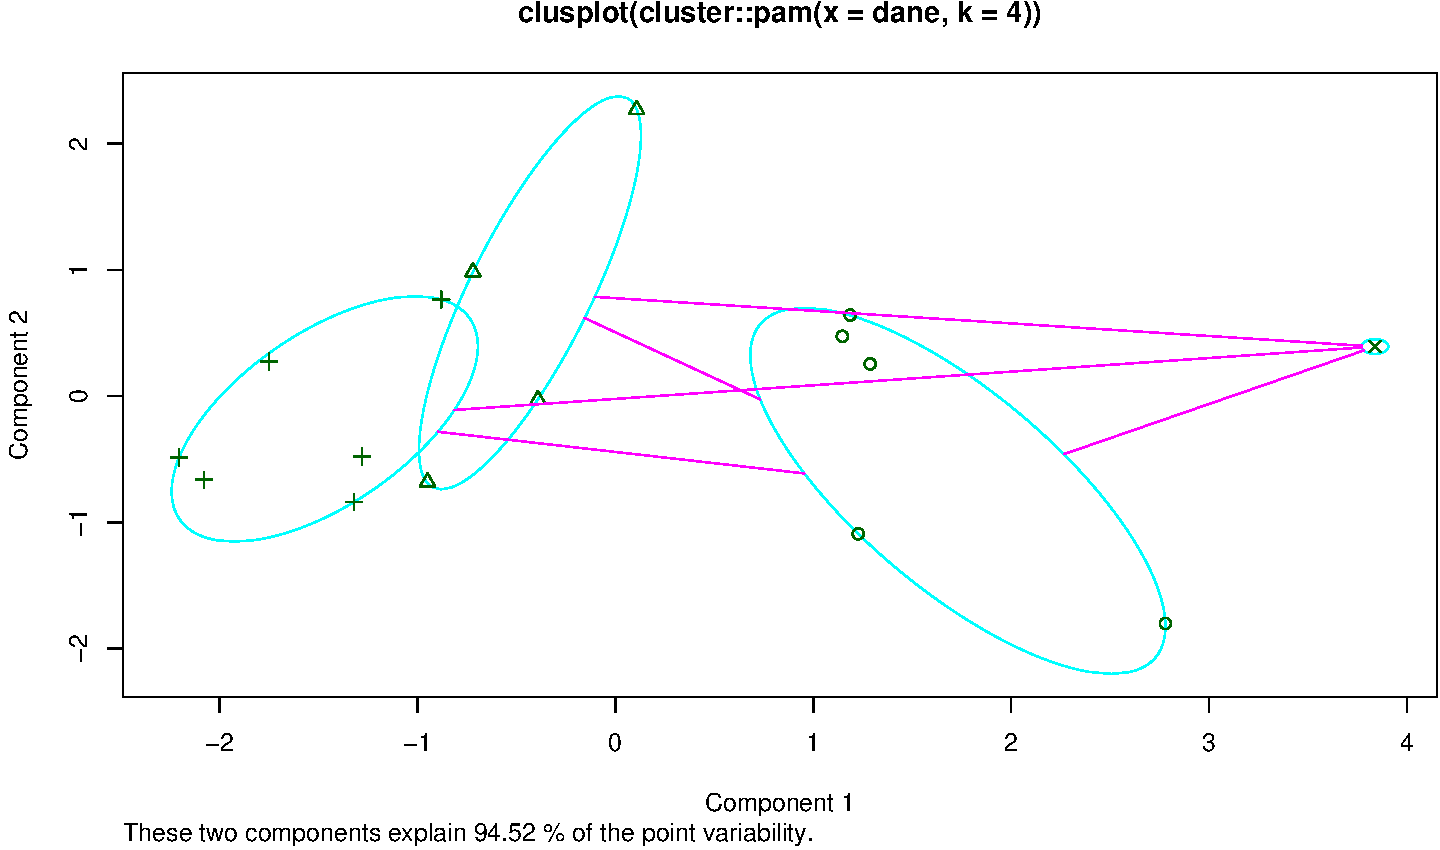
\includegraphics[width=0.7\linewidth]{NaPrzelajR_files/figure-latex/gusp4-1} 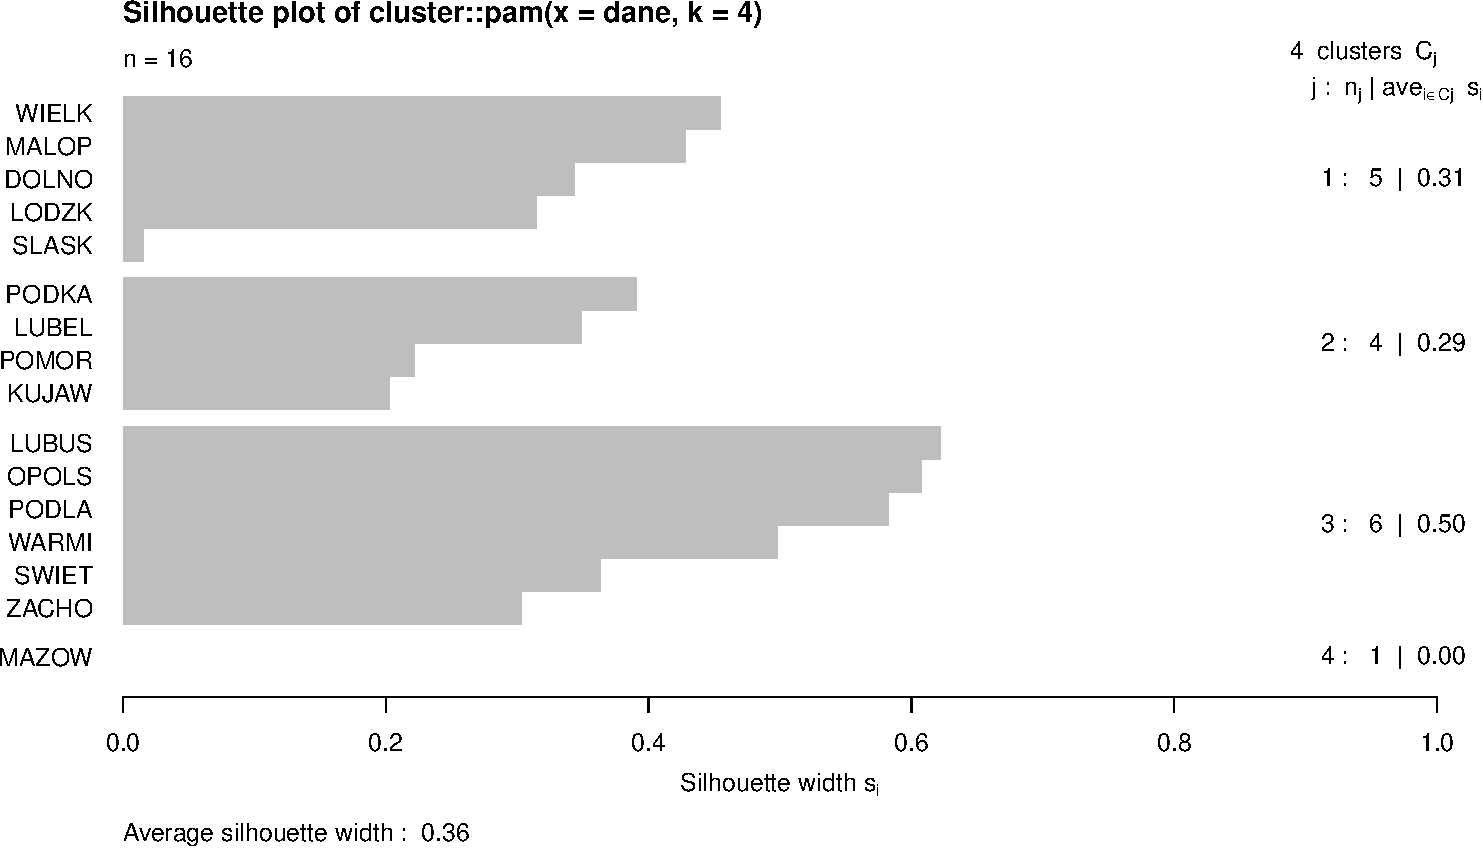
\includegraphics[width=0.7\linewidth]{NaPrzelajR_files/figure-latex/gusp4-2} 

}

\end{figure}

\begin{Shaded}
\begin{Highlighting}[]
\CommentTok{# analiza skupień}
\CommentTok{#}
\end{Highlighting}
\end{Shaded}

\begin{Shaded}
\begin{Highlighting}[]
\KeywordTok{par}\NormalTok{(}\DataTypeTok{mfrow=}\KeywordTok{c}\NormalTok{(}\DecValTok{1}\NormalTok{,}\DecValTok{3}\NormalTok{))}
\NormalTok{h =}\StringTok{ }\KeywordTok{hclust}\NormalTok{(}\KeywordTok{dist}\NormalTok{(dane), }\DataTypeTok{method=}\StringTok{"average"}\NormalTok{)}
\KeywordTok{plot}\NormalTok{(h)}
\NormalTok{h =}\StringTok{ }\KeywordTok{hclust}\NormalTok{(}\KeywordTok{dist}\NormalTok{(dane), }\DataTypeTok{method=}\StringTok{"single"}\NormalTok{)}
\KeywordTok{plot}\NormalTok{(h)}
\NormalTok{h =}\StringTok{ }\KeywordTok{hclust}\NormalTok{(}\KeywordTok{dist}\NormalTok{(dane), }\DataTypeTok{method=}\StringTok{"complete"}\NormalTok{)}
\KeywordTok{plot}\NormalTok{(h)}
\end{Highlighting}
\end{Shaded}

\begin{figure}[h]

{\centering 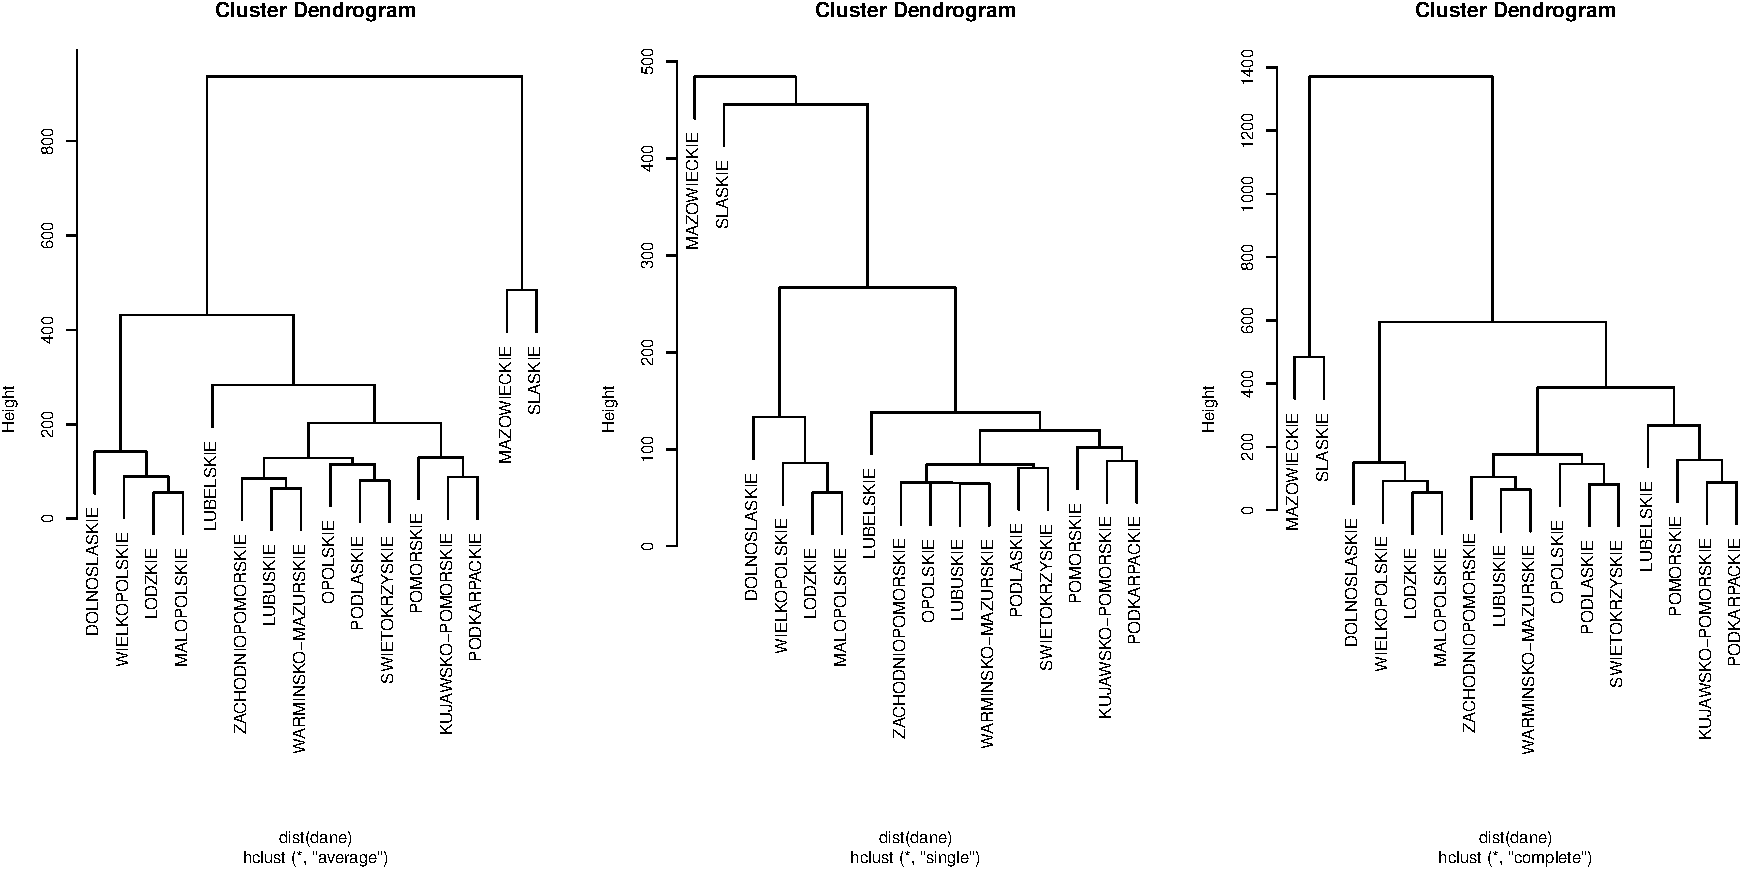
\includegraphics[width=0.7\linewidth]{NaPrzelajR_files/figure-latex/pA-1} 

}

\end{figure}

\begin{Shaded}
\begin{Highlighting}[]
\KeywordTok{library}\NormalTok{(cluster)}
\CommentTok{# cztery przykładowe indeksy}
\NormalTok{mNiep =}\StringTok{ }\KeywordTok{daisy}\NormalTok{(dane)}
\NormalTok{clustGrid =}\StringTok{ }\DecValTok{2}\OperatorTok{:}\DecValTok{14}
\NormalTok{indeksy =}\StringTok{ }\KeywordTok{matrix}\NormalTok{(}\DecValTok{0}\NormalTok{,}\KeywordTok{length}\NormalTok{(clustGrid),}\DecValTok{4}\NormalTok{)}
\NormalTok{indeksy[,}\DecValTok{1}\NormalTok{] =}\StringTok{ }\KeywordTok{sapply}\NormalTok{(clustGrid, }\ControlFlowTok{function}\NormalTok{(x) \{clusterSim}\OperatorTok{::}\KeywordTok{index.G1}\NormalTok{(dane, }\KeywordTok{pam}\NormalTok{(dane, x)}\OperatorTok{$}\NormalTok{clustering)\})}
\NormalTok{indeksy[,}\DecValTok{2}\NormalTok{] =}\StringTok{ }\KeywordTok{sapply}\NormalTok{(clustGrid, }\ControlFlowTok{function}\NormalTok{(x) \{clusterSim}\OperatorTok{::}\KeywordTok{index.Gap}\NormalTok{(dane, }\KeywordTok{cbind}\NormalTok{(}\KeywordTok{pam}\NormalTok{(}
\NormalTok{dane, x)}\OperatorTok{$}\NormalTok{clustering, }\KeywordTok{pam}\NormalTok{(dane, x}\OperatorTok{+}\DecValTok{1}\NormalTok{)}\OperatorTok{$}\NormalTok{clustering))}\OperatorTok{$}\NormalTok{diffu\})}
\NormalTok{indeksy[,}\DecValTok{3}\NormalTok{] =}\StringTok{ }\KeywordTok{sapply}\NormalTok{(clustGrid, }\ControlFlowTok{function}\NormalTok{(x) \{clusterSim}\OperatorTok{::}\KeywordTok{index.G2}\NormalTok{(mNiep, }\KeywordTok{pam}\NormalTok{(dane, x)}\OperatorTok{$}\NormalTok{clustering)\})}
\NormalTok{indeksy[,}\DecValTok{4}\NormalTok{] =}\StringTok{ }\KeywordTok{sapply}\NormalTok{(clustGrid, }\ControlFlowTok{function}\NormalTok{(x) \{clusterSim}\OperatorTok{::}\KeywordTok{index.S}\NormalTok{(mNiep, }\KeywordTok{pam}\NormalTok{(dane, x)}\OperatorTok{$}\NormalTok{clustering)\})}
\KeywordTok{matplot}\NormalTok{(clustGrid, }\KeywordTok{scale}\NormalTok{(indeksy), }\DataTypeTok{type=}\StringTok{"l"}\NormalTok{,}\DataTypeTok{lwd=}\DecValTok{3}\NormalTok{)}
\KeywordTok{legend}\NormalTok{(}\StringTok{"right"}\NormalTok{,}\KeywordTok{c}\NormalTok{(}\StringTok{"G1"}\NormalTok{,}\StringTok{"Gap"}\NormalTok{,}\StringTok{"G2"}\NormalTok{,}\StringTok{"S"}\NormalTok{),}\DataTypeTok{lwd=}\DecValTok{3}\NormalTok{,}\DataTypeTok{bg=}\StringTok{"white"}\NormalTok{,}\DataTypeTok{col=}\DecValTok{1}\OperatorTok{:}\DecValTok{4}\NormalTok{)}
\end{Highlighting}
\end{Shaded}

\begin{figure}[h]

{\centering 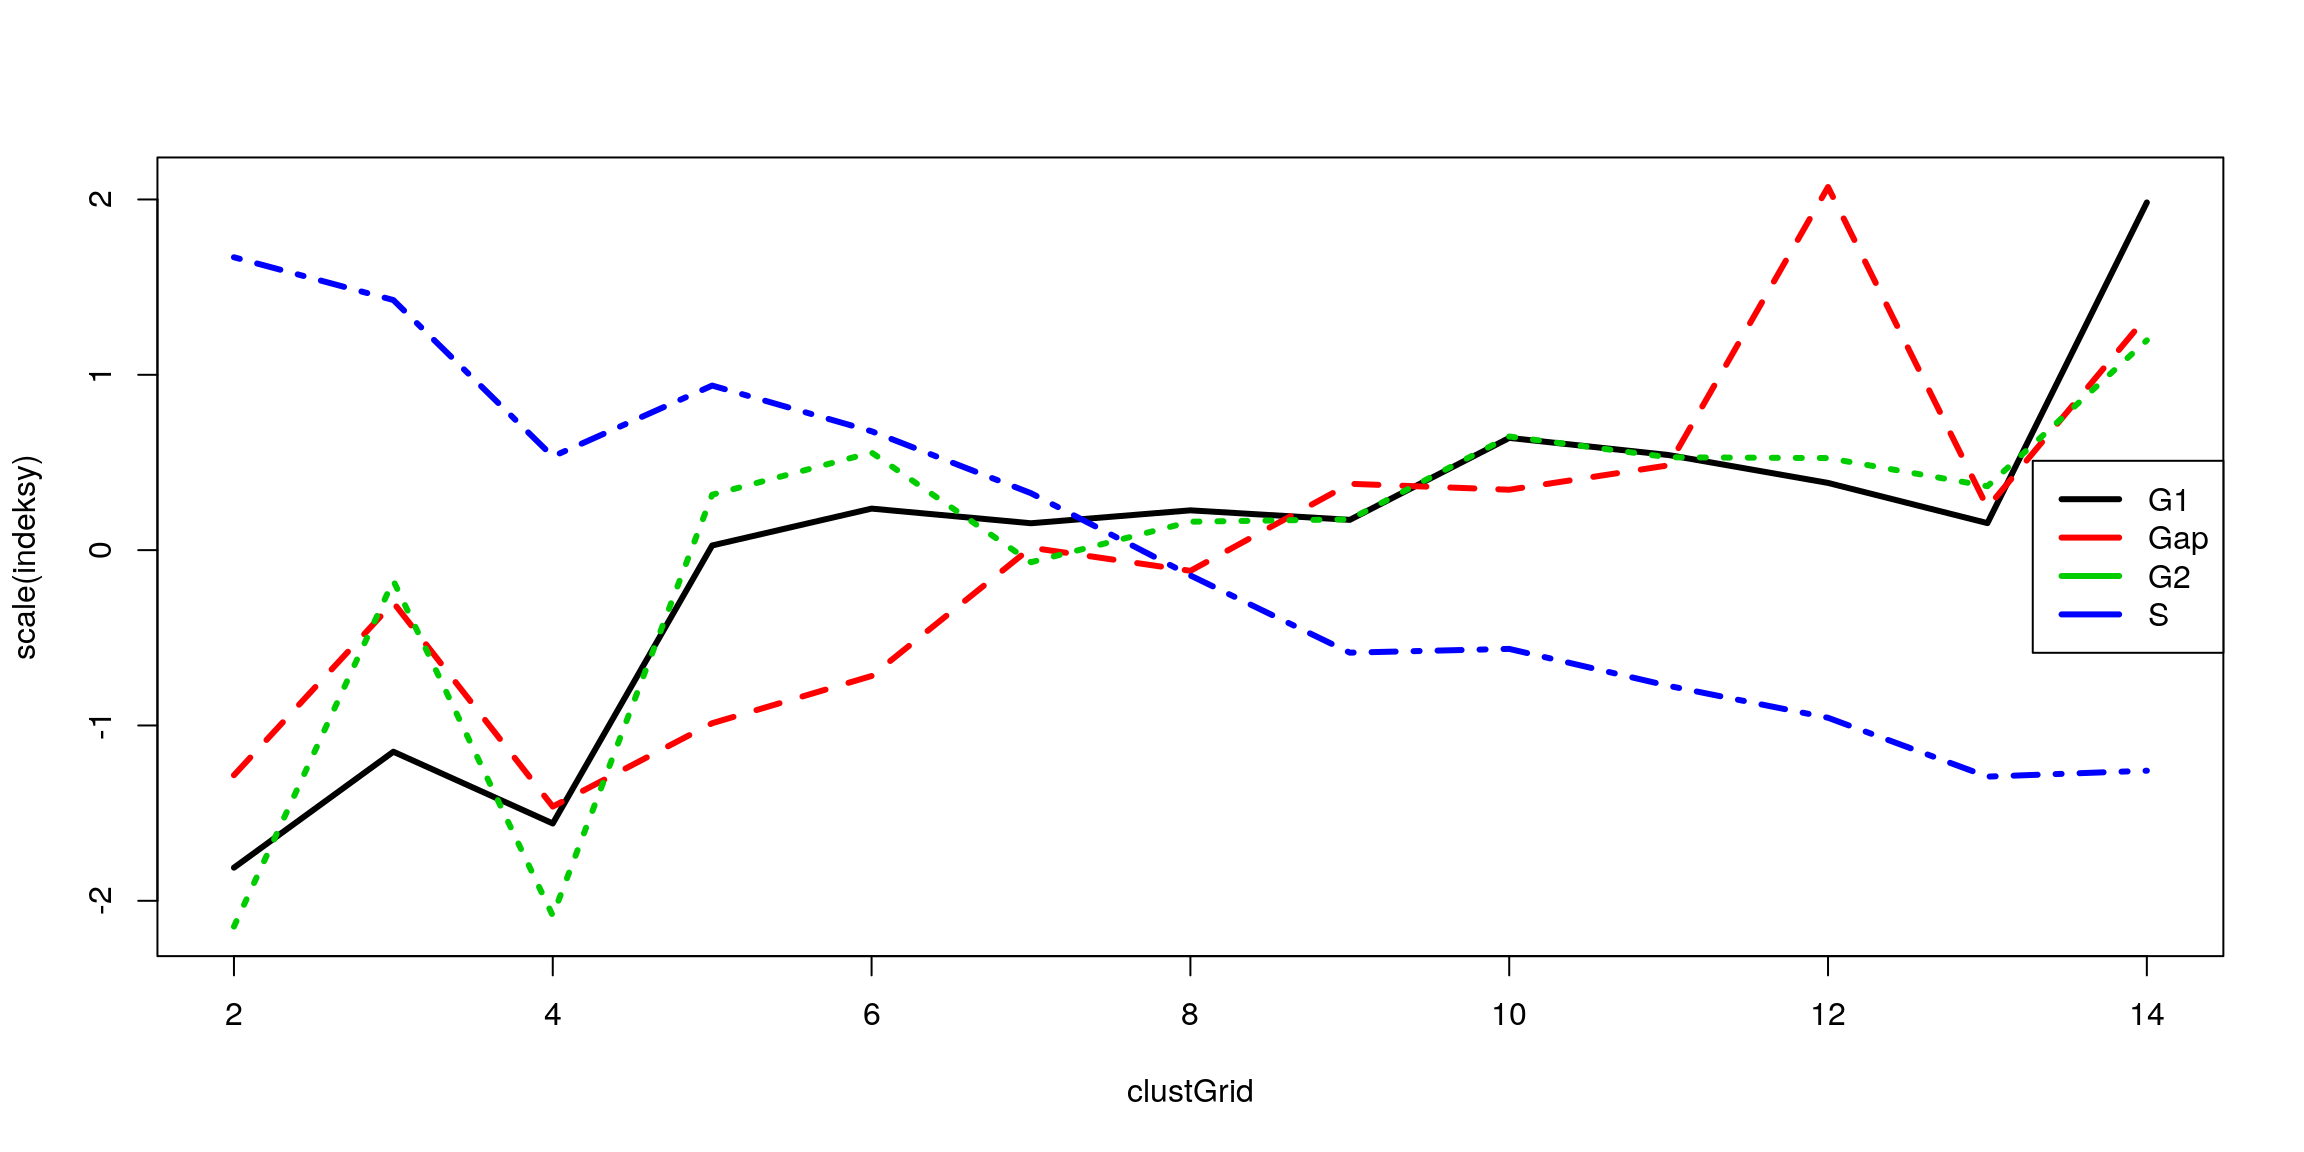
\includegraphics[width=0.7\linewidth]{NaPrzelajR_files/figure-latex/pB-1} 

}

\end{figure}

\begin{Shaded}
\begin{Highlighting}[]
\CommentTok{# cztery metody porównane indeksem G1}
\CommentTok{#}
\NormalTok{clustGrid =}\StringTok{ }\DecValTok{2}\OperatorTok{:}\DecValTok{10}
\NormalTok{indeksy =}\StringTok{ }\KeywordTok{matrix}\NormalTok{(}\DecValTok{0}\NormalTok{,}\KeywordTok{length}\NormalTok{(clustGrid),}\DecValTok{5}\NormalTok{)}
\NormalTok{indeksy[,}\DecValTok{1}\NormalTok{] =}\StringTok{ }\KeywordTok{sapply}\NormalTok{(clustGrid, }\ControlFlowTok{function}\NormalTok{(x) \{clusterSim}\OperatorTok{::}\KeywordTok{index.G1}\NormalTok{(dane,}
              \KeywordTok{pam}\NormalTok{(dane, x)}\OperatorTok{$}\NormalTok{clustering)\})}
\NormalTok{indeksy[,}\DecValTok{2}\NormalTok{] =}\StringTok{ }\KeywordTok{sapply}\NormalTok{(clustGrid, }\ControlFlowTok{function}\NormalTok{(x) \{clusterSim}\OperatorTok{::}\KeywordTok{index.G1}\NormalTok{(dane,}
              \KeywordTok{kmeans}\NormalTok{(dane, x)}\OperatorTok{$}\NormalTok{cluster)\})}
\NormalTok{indeksy[,}\DecValTok{3}\NormalTok{] =}\StringTok{ }\KeywordTok{sapply}\NormalTok{(clustGrid, }\ControlFlowTok{function}\NormalTok{(x) \{clusterSim}\OperatorTok{::}\KeywordTok{index.G1}\NormalTok{(dane,     }
              \KeywordTok{cutree}\NormalTok{(}\KeywordTok{hclust}\NormalTok{(}\KeywordTok{dist}\NormalTok{(dane),}\StringTok{"average"}\NormalTok{), }\DataTypeTok{k =}\NormalTok{ x))\})}
\NormalTok{indeksy[,}\DecValTok{4}\NormalTok{] =}\StringTok{ }\KeywordTok{sapply}\NormalTok{(clustGrid, }\ControlFlowTok{function}\NormalTok{(x) \{clusterSim}\OperatorTok{::}\KeywordTok{index.G1}\NormalTok{(dane,}
              \KeywordTok{cutree}\NormalTok{(}\KeywordTok{hclust}\NormalTok{(}\KeywordTok{dist}\NormalTok{(dane),}\StringTok{"single"}\NormalTok{), }\DataTypeTok{k =}\NormalTok{ x))\})}
\NormalTok{indeksy[,}\DecValTok{5}\NormalTok{] =}\StringTok{ }\KeywordTok{sapply}\NormalTok{(clustGrid, }\ControlFlowTok{function}\NormalTok{(x) \{clusterSim}\OperatorTok{::}\KeywordTok{index.G1}\NormalTok{(dane,}
              \KeywordTok{cutree}\NormalTok{(}\KeywordTok{hclust}\NormalTok{(}\KeywordTok{dist}\NormalTok{(dane),}\StringTok{"complete"}\NormalTok{), }\DataTypeTok{k =}\NormalTok{ x))\})}

\KeywordTok{matplot}\NormalTok{(clustGrid, indeksy, }\DataTypeTok{type=}\StringTok{"l"}\NormalTok{,}\DataTypeTok{lwd=}\DecValTok{3}\NormalTok{)}
\KeywordTok{legend}\NormalTok{(}\StringTok{"right"}\NormalTok{,}\KeywordTok{c}\NormalTok{(}\StringTok{"PAM"}\NormalTok{,}\StringTok{"kmeans"}\NormalTok{,}\StringTok{"hclust av"}\NormalTok{,}\StringTok{"hclust si"}\NormalTok{,}\StringTok{"hclust co"}\NormalTok{),}
       \DataTypeTok{lwd=}\DecValTok{3}\NormalTok{,}\DataTypeTok{bg=}\StringTok{"white"}\NormalTok{,}\DataTypeTok{col=}\DecValTok{1}\OperatorTok{:}\DecValTok{5}\NormalTok{)}
\end{Highlighting}
\end{Shaded}

\begin{figure}[h]

{\centering 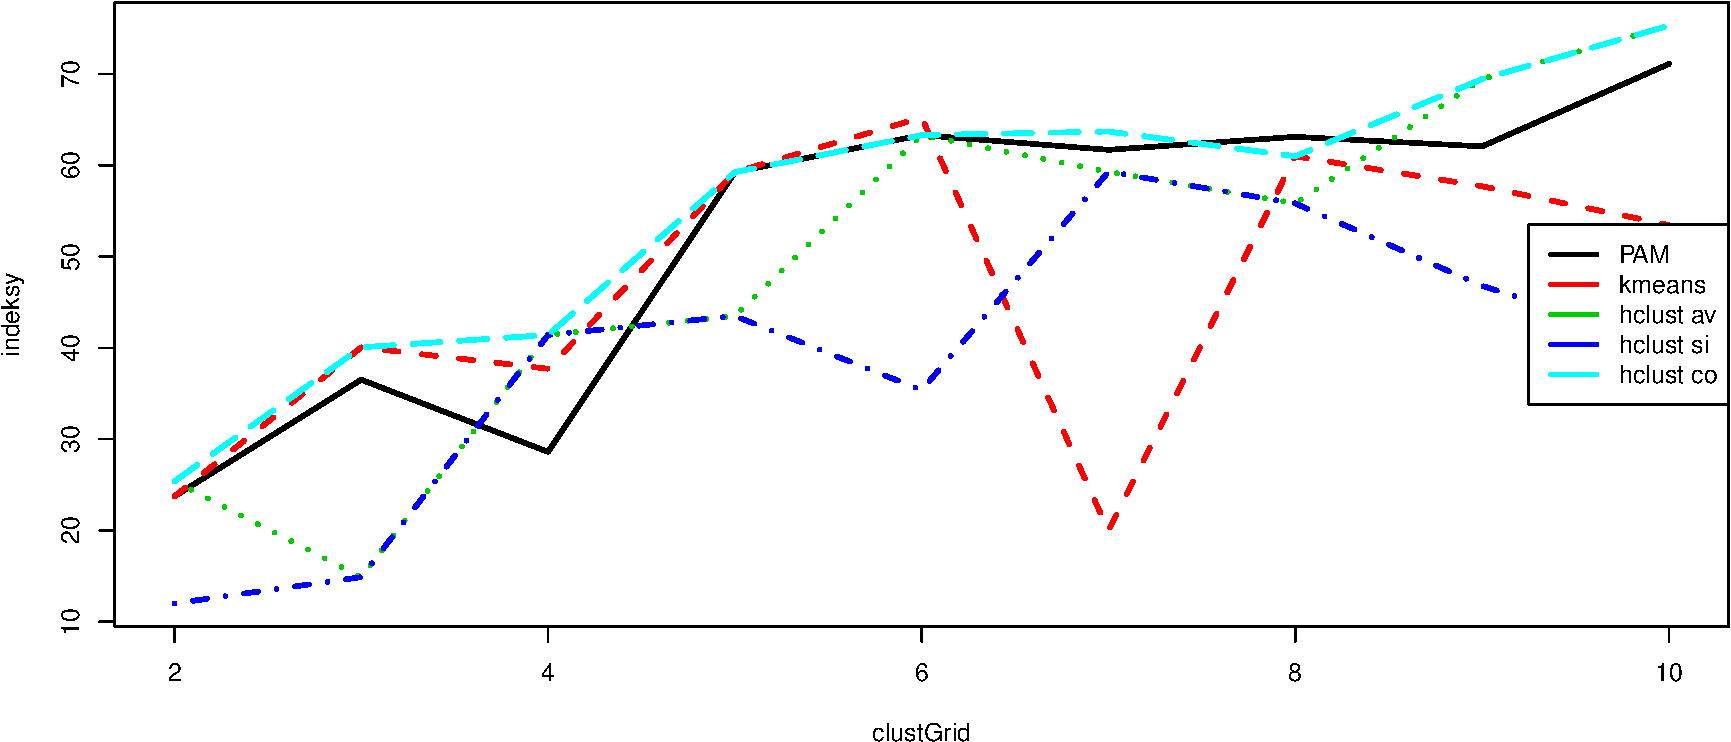
\includegraphics[width=0.7\linewidth]{NaPrzelajR_files/figure-latex/pC-1} 

}

\end{figure}

\begin{Shaded}
\begin{Highlighting}[]
\CommentTok{# profile skupień}
\CommentTok{#}
\NormalTok{gus.p4 =}\StringTok{ }\KeywordTok{pam}\NormalTok{(dane,}\DecValTok{4}\NormalTok{)}\OperatorTok{$}\NormalTok{clustering}
\NormalTok{desc =}\StringTok{ }\NormalTok{clusterSim}\OperatorTok{::}\KeywordTok{cluster.Description}\NormalTok{(dane, gus.p4)}
\end{Highlighting}
\end{Shaded}

\hypertarget{part_36}{%
\section{Case study}\label{part_36}}

\hypertarget{part_4}{%
\chapter{Analiza dyskryminacji}\label{part_4}}

W wielu dziedzinach potrzebne są metody, potrafiące automatycznie przypisać nowy obiekt do jednej z wyróżnionych klas. W medycynie interesować nas może czy
pacjent jest chory, a jeżeli tak to na co (zbiorem klas do którego chcemy przypisać
mogą być możliwe choroby, lub tylko informacja czy jest chory czy nie). W analizie
kredytowej dla firm chcemy przewidzieć czy firma spłaci kredyt czy nie. W analizie
obrazów z fotoradarów policyjnych będzie nas interesowało określenie numeru re-
jestracji samochodu który przekroczył prędkość a również typu pojazdu (w końcu
ograniczenia dla ciężarówek są inne niż dla samochodów).

W rozdziale ?? używaliśmy regresji logistycznej do znalezienia parametrów, które można by wykorzystać w określeniu ryzyka pojawienia się wznowienia choroby
u operowanych pacjentek. Okazuje się wiec, że regresja logistyczna jest klasyfikatorem, pozwalającym na przypisanie nowego obiektu do jednej z dwóch klas. Poniżej
przedstawimy szereg funkcji implementujących inne popularne metody analizy dyskryminacji.

Celem procesu dyskryminacji (nazywanego też klasyfikacją, uczeniem z nauczycielem lub uczeniem z nadzorem) jest zbudowanie reguły, potrafiącej przypisywać
możliwie dokładnie nowe obiekty do znanych klas. W przypadku większości metod
możliwe jest klasyfikowanie do więcej niż dwie klasy.

\hypertarget{part_41}{%
\section{Dyskryminacja liniowa i kwadratowa}\label{part_41}}

Dyskryminacja liniowa, a więc metoda wyznaczania (hiper)płaszczyzn separujących
obiekty różnych klas, jest dostępna w funkcji \texttt{lda(MASS)}. Rozszerzeniem tej metody jest dyskryminacja kwadratowa, umożliwiająca dyskryminacje powierzchniami,
w opisie których mogą pojawić się człony stopnia drugiego. Metoda klasyfikacji kwadratowej jest dostępna w funkcji \texttt{qda(MASS)}. Wynikami obu funkcji jest klasyfikator,
wyznaczony na zbiorze uczącym. Aby użyć go do predykcji klas dla nowych obiektów
możemy wykorzystać przeciążoną funkcje \texttt{predict()}.

Poniżej przedstawiamy przykład użycia funkcji \texttt{lda()}. Z funkcji \texttt{qda()} korzysta
się w identyczny sposób. Na potrzeby przykładu wykorzystaliśmy zbiór danych do-
tyczących występowania cukrzycy u Indian Pima, ten zbiór danych jest dostępny
w zbiorze \texttt{PimaIndiansDiabetes2(mlbench)}. Interesować nas będą dwie zmienne
z tego zbioru danych, opisujące poziom glukozy i insuliny, w zbiorze danych jest
znacznie więcej zmiennych, ale na potrzeby wizualizacji wybraliśmy tę parę. Na bazie tych dwóch zmiennych będziemy badać skuteczność oceny czy dana osoba jest
cukrzykiem z wykorzystaniem obu algorytmów klasyfikacji. Zbiór danych podzielimy na dwie części, uczącą i testową. Klasyfikator zostanie „nauczony'' na zbiorze
uczących, a później będziemy weryfikować jego właściwości na zbiorze testowym.
Pierwszym argumentem funkcji \texttt{lda()} jest zbiór zmiennych na bazie których
budowany będzie klasyfikator (ramka danych lub macierz). Drugim argumentem
grouping jest wektor określający klasy kolejnych obiektów. Kolejnym wykorzystanym poniżej argumentem jest subset, określający indeksy obiektów, na bazie których budowany ma być klasyfikator. Jeżeli argument subset nie będzie podany, to
do konstrukcji klasyfikatora wykorzystane będą wszystkie obiekty. Jako pierwszy
argument funkcji \texttt{lda()} można również podać również formułę, określającą, które
zmienne mają być użyte do konstrukcji klasyfikatora a która zmienna opisuje klasy.

\begin{Shaded}
\begin{Highlighting}[]
\KeywordTok{library}\NormalTok{(}\StringTok{"mlbench"}\NormalTok{)}
\CommentTok{# wczytujemy zbiór danych z pakietu mlbench, usuwamy brakujące dane i}
\CommentTok{# logarytmujemy poziom insuliny}
\KeywordTok{data}\NormalTok{(PimaIndiansDiabetes2)}
\NormalTok{dane =}\StringTok{ }\KeywordTok{na.omit}\NormalTok{(PimaIndiansDiabetes2)[,}\KeywordTok{c}\NormalTok{(}\DecValTok{2}\NormalTok{,}\DecValTok{5}\NormalTok{,}\DecValTok{9}\NormalTok{)]}
\NormalTok{dane[,}\DecValTok{2}\NormalTok{] =}\StringTok{ }\KeywordTok{log}\NormalTok{(dane[,}\DecValTok{2}\NormalTok{])}
\CommentTok{# zbiór danych chcemy podzielić na dwie części, uczącą i testową,}
\CommentTok{# funkcją sample wylosujemy indeksy obiektów, które trafia do zbioru uczącego}
\NormalTok{zbior.uczacy =}\StringTok{ }\KeywordTok{sample}\NormalTok{(}\DecValTok{1}\OperatorTok{:}\KeywordTok{nrow}\NormalTok{(dane), }\KeywordTok{nrow}\NormalTok{(dane)}\OperatorTok{/}\DecValTok{2}\NormalTok{, }\OtherTok{FALSE}\NormalTok{)}
\CommentTok{# wywołujemy funkcję lda}
\NormalTok{klasyfikatorLDA =}\StringTok{ }\KeywordTok{lda}\NormalTok{(dane[,}\DecValTok{1}\OperatorTok{:}\DecValTok{2}\NormalTok{], }\DataTypeTok{grouping =}\NormalTok{ dane[,}\DecValTok{3}\NormalTok{], }\DataTypeTok{subset=}\NormalTok{zbior.uczacy)}
\CommentTok{# jak wygląda wynik w środku?}
\KeywordTok{str}\NormalTok{(klasyfikatorLDA)}
\end{Highlighting}
\end{Shaded}

\begin{verbatim}
## List of 8
##  $ prior  : Named num [1:2] 0.648 0.352
##   ..- attr(*, "names")= chr [1:2] "neg" "pos"
##  $ counts : Named int [1:2] 127 69
##   ..- attr(*, "names")= chr [1:2] "neg" "pos"
##  $ means  : num [1:2, 1:2] 112.39 142.74 4.63 5.08
##   ..- attr(*, "dimnames")=List of 2
##   .. ..$ : chr [1:2] "neg" "pos"
##   .. ..$ : chr [1:2] "glucose" "insulin"
##  $ scaling: num [1:2, 1] 0.0366 -0.0169
##   ..- attr(*, "dimnames")=List of 2
##   .. ..$ : chr [1:2] "glucose" "insulin"
##   .. ..$ : chr "LD1"
##  $ lev    : chr [1:2] "neg" "pos"
##  $ svd    : num 7.37
##  $ N      : int 196
##  $ call   : language lda(x = dane[, 1:2], grouping = dane[, 3], subset = zbior.uczacy)
##  - attr(*, "class")= chr "lda"
\end{verbatim}

Zbudowanie klasyfikatora to dopiero pierwszy krok, kolejnym jest jego ocena.
Na bazie obserwacji niewykorzystanych do budowania klasyfikatora zbadamy jaka
była zgodność klasyfikatora z rzeczywistymi danymi (ponieważ zbiór uczący wybraliśmy losowo, to dla różnych powtórzeń otrzymalibyśmy inny błąd klasyfikacji).
Do klasyfikacji nowych obiektów użyjemy funkcji \texttt{predict()}. Jest to funkcja przeciążona, działająca dla większości klasyfikatorów. Wynikiem tej funkcji mogą być
prognozowane klasy dla nowych obserwacji, lub też prawdopodobieństwa a posteriori przynależności do danej klasy.

\begin{Shaded}
\begin{Highlighting}[]
\CommentTok{# używając metody predict wykonujemy klasyfikacje obiektów ze zbioru testowego}
\NormalTok{oceny =}\StringTok{ }\KeywordTok{predict}\NormalTok{(klasyfikatorLDA, }\DataTypeTok{newdata=}\NormalTok{dane[}\OperatorTok{-}\NormalTok{zbior.uczacy,}\DecValTok{1}\OperatorTok{:}\DecValTok{2}\NormalTok{])}
\CommentTok{# jak wyglądają wyniki? Pole $class wskazuje na przewidzianą klasę, pole}
\CommentTok{# $posterior określa wyznaczone prawdopodobieństwo przynależności do}
\CommentTok{# każdej z klas, na podstawie tej wartości obiekt był przypisywany do}
\CommentTok{# bardziej prawdopodobnej dla niego klasy}
\KeywordTok{str}\NormalTok{(oceny)}
\end{Highlighting}
\end{Shaded}

\begin{verbatim}
## List of 3
##  $ class    : Factor w/ 2 levels "neg","pos": 1 1 2 2 1 2 1 1 2 2 ...
##  $ posterior: num [1:196, 1:2] 0.897 0.931 0.103 0.138 0.831 ...
##   ..- attr(*, "dimnames")=List of 2
##   .. ..$ : chr [1:196] "4" "7" "9" "14" ...
##   .. ..$ : chr [1:2] "neg" "pos"
##  $ x        : num [1:196, 1] -1.242 -1.644 2.679 2.378 -0.728 ...
##   ..- attr(*, "dimnames")=List of 2
##   .. ..$ : chr [1:196] "4" "7" "9" "14" ...
##   .. ..$ : chr "LD1"
\end{verbatim}

\begin{Shaded}
\begin{Highlighting}[]
\CommentTok{# porównajmy macierzą kontyngencji oceny i rzeczywiste etykietki dla kolejnych obiektów}
\KeywordTok{table}\NormalTok{(}\DataTypeTok{predykcja =}\NormalTok{ oceny}\OperatorTok{$}\NormalTok{class, }\DataTypeTok{prawdziwe =}\NormalTok{ dane[}\OperatorTok{-}\NormalTok{zbior.uczacy,}\DecValTok{3}\NormalTok{])}
\end{Highlighting}
\end{Shaded}

\begin{verbatim}
##          prawdziwe
## predykcja neg pos
##       neg 122  27
##       pos  13  34
\end{verbatim}

W powyższym przykładzie w ostatnim poleceniu wyznaczyliśmy tablice kontyngencji dla wyników. Na bazie tak otrzymanej tablicy kontyngencji można wyznaczyć błąd predykcji. Jest wiele wskaźników opisujących błąd predykcji, począwszy
od popularnych: czułość (ang. sensitivity \texttt{TP/(TP+FN)} opisuje jaki procent chorych
zostanie poprawnie zdiagnozowanych jako chorzy), specyficzność (ang. (Specifity)
\texttt{TN/(TN+FP)} określa jaki procent zdrowych zostanie poprawnie zdiagnozowanych jako zdrowi), przez mniej popularne aż po takie o których mało kto słyszał (np. mutual
information, współczynnik \(\phi\) itp.). Bogata lista takich współczynników wymieniona jest w opisie funkcji \texttt{performance(ROCR)} (definiując błąd klasyfikacji używa się
oznaczeń \texttt{TP}, \texttt{TN}, \texttt{FP}, \texttt{FN} określających kolejno liczbę poprawnie wykrytych sygnałów
pozytywnych, poprawnie wykrytych braków sygnału, fałszywie wykrytych sygnałów
pozytywnych oraz fałszywie wykrytych braków sygnałów. W powyższym przypadku
czułość wyniosła \(31/(31+29)\approx0,517\) a specyficzność \(115/(115+21)\approx 0,846\).

Jeżeli już jesteśmy przy pakiecie ROCR to na przykładzie przedstawimy w jaki sposób wyznaczać krzywe ROC dla klasyfikatorów. Proszę zauważyć, że funkcja
\texttt{predict()} poza ocenionymi klasami jako wynik przekazuje również prawdopodobieństwo przynależności do jednej z klas (pole \texttt{posterior} wyniku funkcji \texttt{predict()}).
Krzywa ROC to zbiór punktów wyznaczonych dla różnych poziomów odcięcia (ang.
threshold) dla wspomnianego prawdopodobieństwa przynależności do jednej z klas.
Współrzędne każdego punktu to czułość i specyficzność (dokładniej rzecz biorąc
1-specyficzność) otrzymana dla zadanego punktu odcięcia.

Poniżej przykład użycia funkcji z pakietu \texttt{ROCR}, służącej do rysowania krzywych
ROC i innych o podobnych właściwościach. Wynik graficzny przedstawiony jest na
rysunku \ref{fig:ad41}. Na osiach tego wykresu mogą być przedstawiane różne miary dokładności klasyfikacji, w zależności od argumentów funkcji \texttt{performance()}.

\begin{Shaded}
\begin{Highlighting}[]
\CommentTok{# wyznaczamy obiekt klasy prediction, zawierający informacje o prawdziwych}
\CommentTok{# klasach, i prawdopodobieństwu przynależności do wybranej klasy}
\NormalTok{pred <-}\StringTok{ }\NormalTok{ROCR}\OperatorTok{::}\KeywordTok{prediction}\NormalTok{(oceny}\OperatorTok{$}\NormalTok{posterior[,}\DecValTok{2}\NormalTok{], dane[}\OperatorTok{-}\NormalTok{zbior.uczacy,}\DecValTok{3}\NormalTok{])}
\CommentTok{# wyznaczamy i wyrysowujemy wybrane miary dobroci klasyfikacji}
\NormalTok{perf <-}\StringTok{ }\NormalTok{ROCR}\OperatorTok{::}\KeywordTok{performance}\NormalTok{(pred, }\StringTok{"sens"}\NormalTok{, }\StringTok{"spec"}\NormalTok{)}
\KeywordTok{par}\NormalTok{(}\DataTypeTok{mfcol=}\KeywordTok{c}\NormalTok{(}\DecValTok{1}\NormalTok{,}\DecValTok{2}\NormalTok{))}
\KeywordTok{plot}\NormalTok{(perf}\OperatorTok{@}\NormalTok{x.values[[}\DecValTok{1}\NormalTok{]], perf}\OperatorTok{@}\NormalTok{y.values[[}\DecValTok{1}\NormalTok{]],}\DataTypeTok{type=}\StringTok{"l"}\NormalTok{)}
\NormalTok{perf <-}\StringTok{ }\NormalTok{ROCR}\OperatorTok{::}\KeywordTok{performance}\NormalTok{(pred, }\StringTok{"prec"}\NormalTok{, }\StringTok{"rec"}\NormalTok{)}
\KeywordTok{plot}\NormalTok{(perf}\OperatorTok{@}\NormalTok{x.values[[}\DecValTok{1}\NormalTok{]], perf}\OperatorTok{@}\NormalTok{y.values[[}\DecValTok{1}\NormalTok{]],}\DataTypeTok{type=}\StringTok{"l"}\NormalTok{)}
\end{Highlighting}
\end{Shaded}

\begin{figure}[h]

{\centering 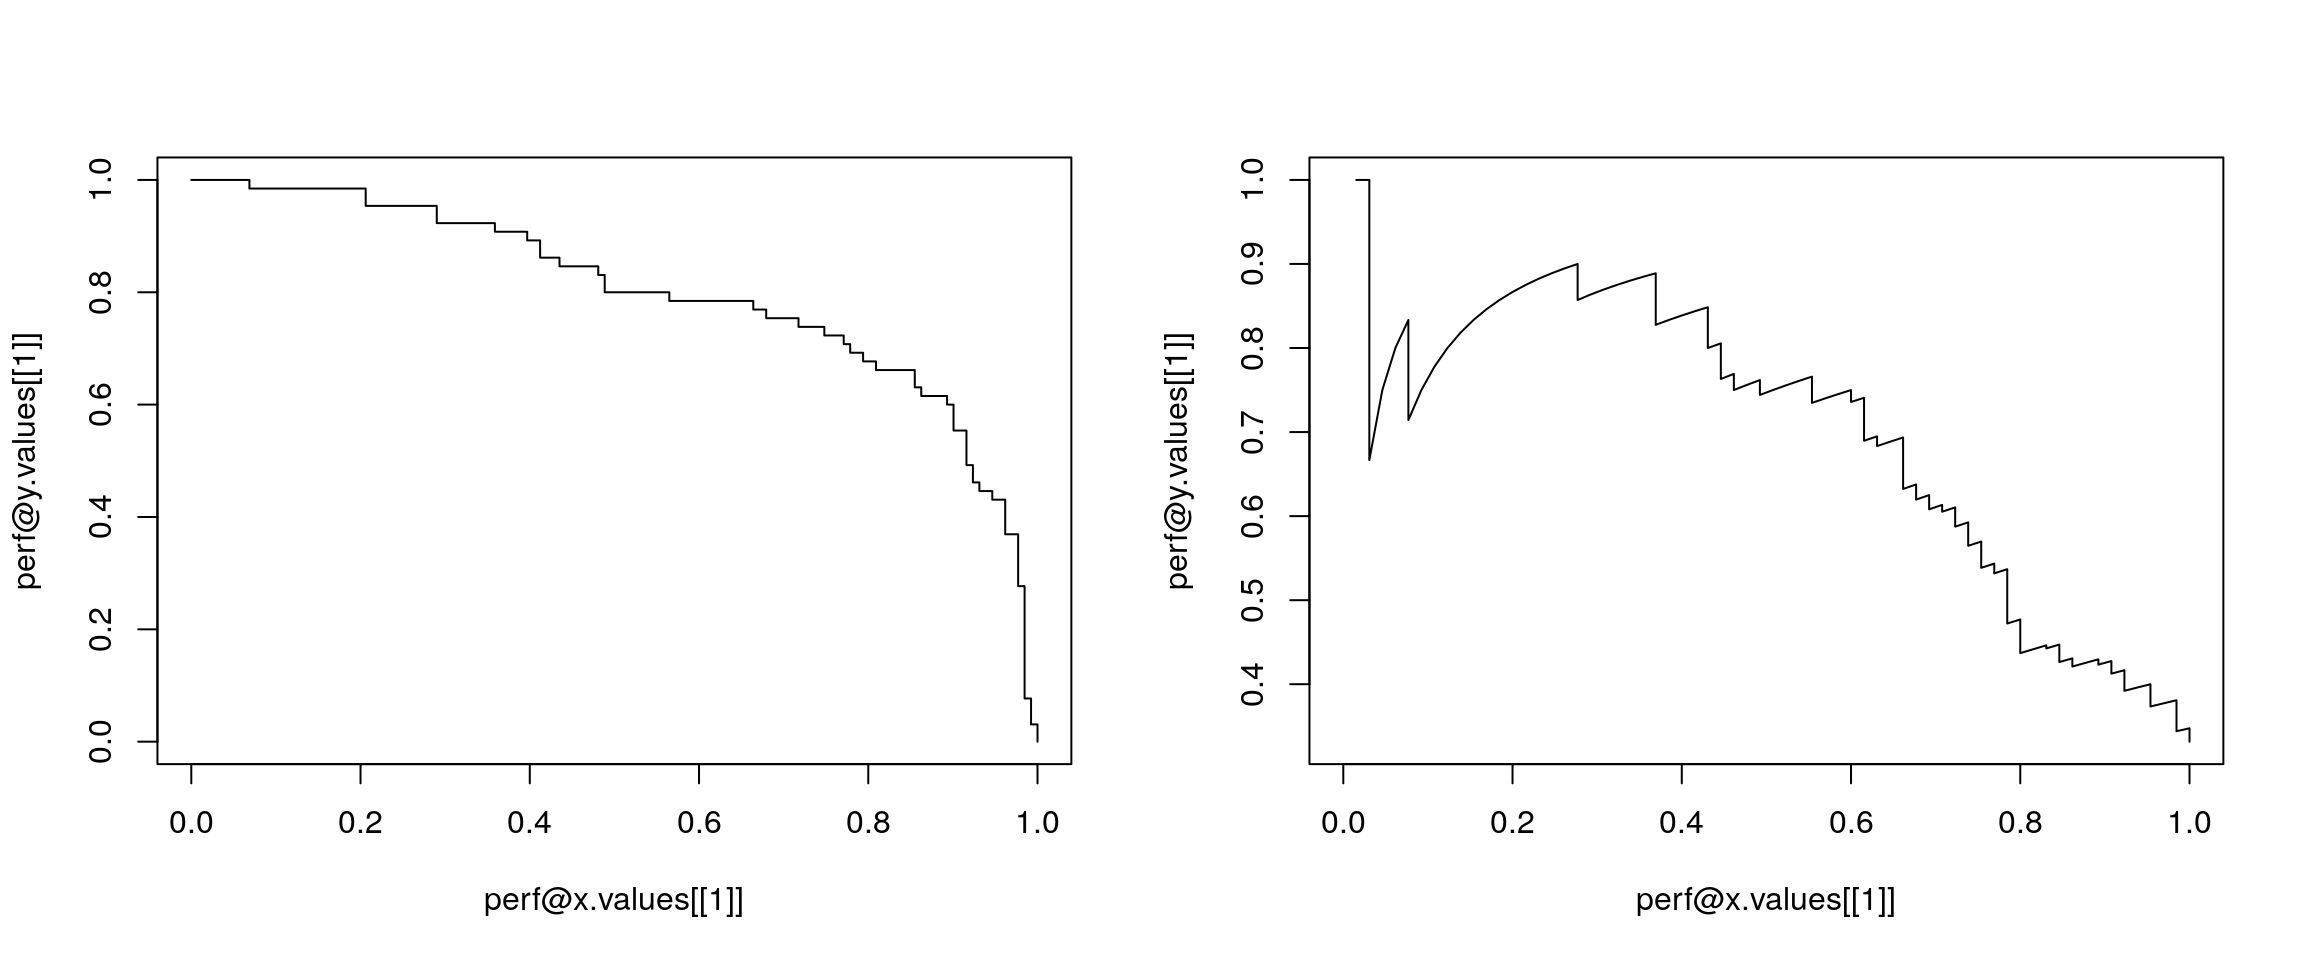
\includegraphics[width=1\linewidth]{NaPrzelajR_files/figure-latex/ad41-1} 

}

\caption{Wykres zależności czułości od specyficzności oraz miary prediction od recall dla klasyfikacji z użyciem funkcji lda().}\label{fig:ad41}
\end{figure}

Na rysunku \ref{fig:ad42} przedstawiamy kształty obszarów decyzyjnych dla obu klasyfikatorów (do wyznaczania obszarów decyzyjnych można się posłużyć funkcją \texttt{partimat(klaR)}
lub \texttt{drawparti(klaR)}). Obszary decyzyjne wyznaczane są dla wytrenowanego klasyfikatora, przedstawiają do której klasy zostałby przypisany punkt o określonych
współrzędnych. Osoby chore na cukrzyce oznaczane są czarnymi krzyżykami, osoby
zdrowe czerwonymi okręgami. Punkty w których przewidzianą klasą była by cukrzyca zaznaczone są ciemnoszarym kolorem a punkty dla których klasyfikowalibyśmy
do grona osób zdrowych zaznaczono jaśniejszym szarym kolorem.

\begin{Shaded}
\begin{Highlighting}[]
\NormalTok{PimaIndiansDiabetes2 =}\StringTok{ }\KeywordTok{na.omit}\NormalTok{(PimaIndiansDiabetes2)}
\NormalTok{dat =}\StringTok{ }\NormalTok{PimaIndiansDiabetes2[,}\KeywordTok{c}\NormalTok{(}\DecValTok{2}\NormalTok{,}\DecValTok{5}\NormalTok{)]}
\NormalTok{dat[,}\DecValTok{2}\NormalTok{] =}\StringTok{ }\KeywordTok{log}\NormalTok{(dat[,}\DecValTok{2}\NormalTok{])}

\KeywordTok{colnames}\NormalTok{(dat) =}\StringTok{  }\KeywordTok{c}\NormalTok{(}\StringTok{"glucose"}\NormalTok{, }\StringTok{"log(insulin)"}\NormalTok{)}
\NormalTok{klasa =}\StringTok{ }\KeywordTok{as.numeric}\NormalTok{(PimaIndiansDiabetes2}\OperatorTok{$}\NormalTok{diabetes)}

\NormalTok{seqx =}\StringTok{ }\KeywordTok{seq}\NormalTok{(}\DecValTok{30}\NormalTok{,}\DecValTok{210}\NormalTok{,}\DecValTok{2}\NormalTok{)}
\NormalTok{seqy =}\StringTok{ }\KeywordTok{seq}\NormalTok{(}\FloatTok{2.5}\NormalTok{,}\DecValTok{7}\NormalTok{,}\FloatTok{0.07}\NormalTok{)}
\NormalTok{siata =}\StringTok{ }\KeywordTok{as.data.frame}\NormalTok{(}\KeywordTok{expand.grid}\NormalTok{(seqx, seqy))}
\KeywordTok{colnames}\NormalTok{(siata) =}\KeywordTok{c}\NormalTok{(}\StringTok{"glucose"}\NormalTok{, }\StringTok{"log(insulin)"}\NormalTok{)}

\NormalTok{kol  =}\StringTok{ }\KeywordTok{c}\NormalTok{(}\StringTok{"grey90"}\NormalTok{, }\StringTok{"grey70"}\NormalTok{)}
\NormalTok{kol2  =}\StringTok{ }\KeywordTok{c}\NormalTok{(}\StringTok{"red"}\NormalTok{, }\StringTok{"black"}\NormalTok{)}
\KeywordTok{par}\NormalTok{(}\DataTypeTok{mfcol=}\KeywordTok{c}\NormalTok{(}\DecValTok{1}\NormalTok{,}\DecValTok{2}\NormalTok{))}
\NormalTok{klasyfikatorLDA =}\StringTok{ }\NormalTok{MASS}\OperatorTok{::}\KeywordTok{lda}\NormalTok{(dat, klasa)}
\NormalTok{wub =}\StringTok{ }\KeywordTok{predict}\NormalTok{(klasyfikatorLDA, }\DataTypeTok{newdata=}\NormalTok{siata)}

\KeywordTok{plot}\NormalTok{(siata, }\DataTypeTok{col=}\NormalTok{kol[}\KeywordTok{as.numeric}\NormalTok{(wub}\OperatorTok{$}\NormalTok{class)],}
     \DataTypeTok{pch=}\DecValTok{15}\NormalTok{,}\DataTypeTok{xlim=}\KeywordTok{range}\NormalTok{(dat[,}\DecValTok{1}\NormalTok{]),}\DataTypeTok{ylim=}\KeywordTok{range}\NormalTok{(dat[,}\DecValTok{2}\NormalTok{]), }\DataTypeTok{main=}\StringTok{"lda()"}\NormalTok{)}
\KeywordTok{points}\NormalTok{(dat,}\DataTypeTok{pch=}\KeywordTok{c}\NormalTok{(}\DecValTok{1}\NormalTok{,}\DecValTok{4}\NormalTok{)[klasa], }\DataTypeTok{cex=}\DecValTok{1}\NormalTok{, }\DataTypeTok{col=}\NormalTok{kol2[klasa], }\DataTypeTok{lwd=}\DecValTok{2}\NormalTok{)}

\NormalTok{klasyfikatorLDA =}\StringTok{ }\NormalTok{MASS}\OperatorTok{::}\KeywordTok{qda}\NormalTok{(dat, klasa)}
\NormalTok{wub =}\StringTok{ }\KeywordTok{predict}\NormalTok{(klasyfikatorLDA, }\DataTypeTok{newdata=}\NormalTok{siata)}

\KeywordTok{plot}\NormalTok{(siata, }\DataTypeTok{col=}\NormalTok{kol[}\KeywordTok{as.numeric}\NormalTok{(wub}\OperatorTok{$}\NormalTok{class)],}
     \DataTypeTok{pch=}\DecValTok{15}\NormalTok{,}\DataTypeTok{xlim=}\KeywordTok{range}\NormalTok{(dat[,}\DecValTok{1}\NormalTok{]),}\DataTypeTok{ylim=}\KeywordTok{range}\NormalTok{(dat[,}\DecValTok{2}\NormalTok{]), }\DataTypeTok{main=}\StringTok{"qda()"}\NormalTok{)}
\KeywordTok{points}\NormalTok{(dat,}\DataTypeTok{pch=}\KeywordTok{c}\NormalTok{(}\DecValTok{1}\NormalTok{,}\DecValTok{4}\NormalTok{)[klasa], }\DataTypeTok{cex=}\DecValTok{1}\NormalTok{, }\DataTypeTok{col=}\NormalTok{kol2[klasa], }\DataTypeTok{lwd=}\DecValTok{2}\NormalTok{)}
\end{Highlighting}
\end{Shaded}

\begin{figure}[h]

{\centering 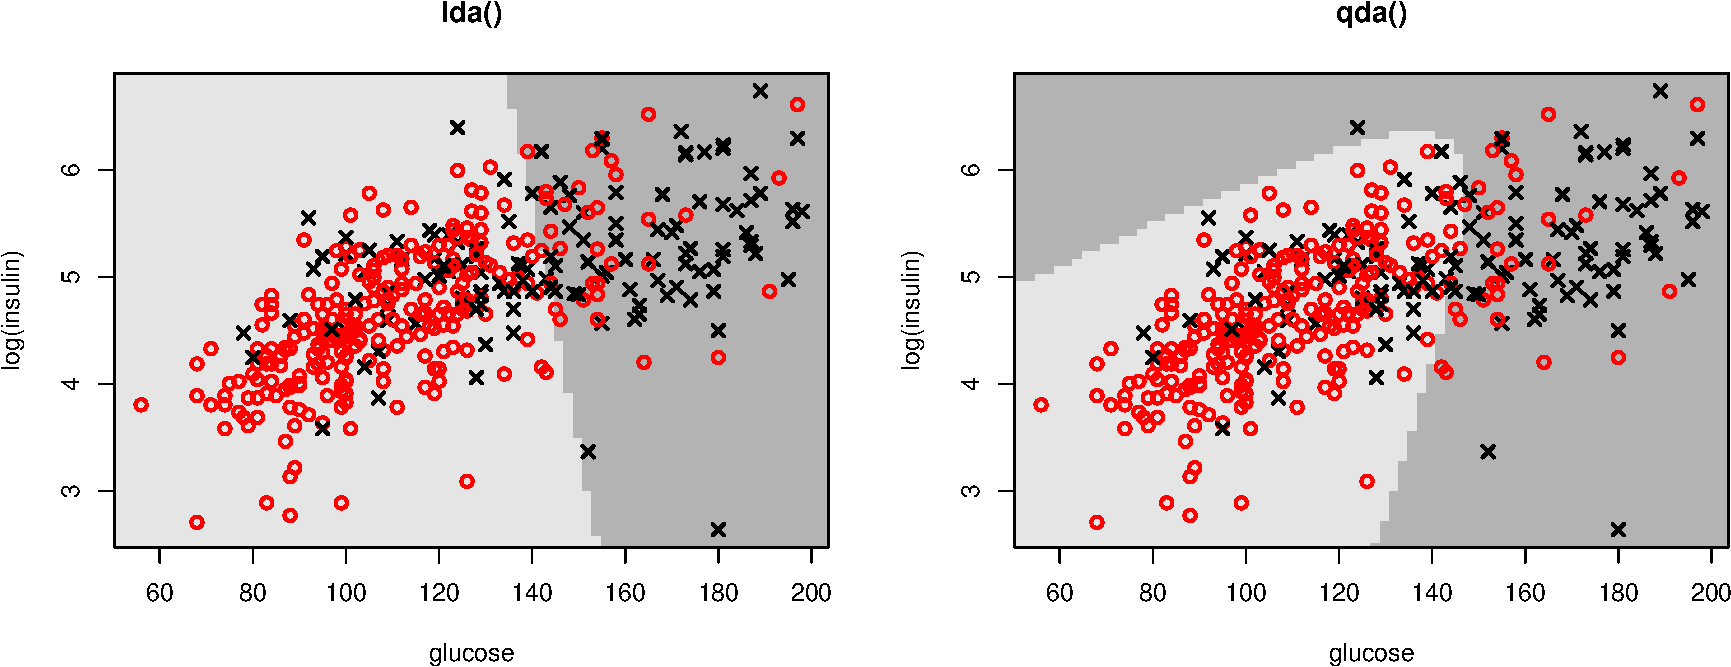
\includegraphics[width=1\linewidth]{NaPrzelajR_files/figure-latex/ad42-1} 

}

\caption{Przykładowe obszary decyzyjne dla liniowej i kwadratowej dyskryminacji dostępne w funkcjach lda() o qda().}\label{fig:ad42}
\end{figure}

\hypertarget{part_42}{%
\section{Metoda najbliższych sąsiadów}\label{part_42}}

Bardzo popularną metodą klasyfikacji jest metoda k-sąsiadów. Idea jej działania
jest prosta i intuicyjna. Nowemu obiektowi przypisuje się klasę, która występuje
najczęściej wśród jego k sąsiadów (k najbliższych obiektów znajdujących się w zbiorze uczącym, najbliższych w sensie określonej miary odległości). Ten klasyfikator
dostępny jest w różnych funkcjach, począwszy od \texttt{knn(class)} (zwykły klasyfikator najbliższych sąsiadów), przez \texttt{kknn(kknn)} (ważony klasyfikator k-sąsiadów) oraz
\texttt{knncat(knncat)} (klasyfikator k-sąsiadów, również dla zmiennych jakościowych).
Poniżej przedstawimy implementację metody k-sąsiadów z funkcji \texttt{ipredknn(ipred)}.
Na rysunku \ref{fig:ad43} prezentujemy obszary decyzyjne wyznaczone dla różnej liczby sąsiadów (odpowiednio k=3 i k=21) w omawianym zagadnieniu klasyfikacji na osoby
zdrowe i chore na cukrzycę. Ponieważ metoda k-sąsiadów bazuje silnie na odległościach pomiędzy obiektami (jakoś trzeba mierzyć odległość od sąsiadów), przed rozpoczęciem obliczeń wykonamy skalowanie danych.

\begin{Shaded}
\begin{Highlighting}[]
\CommentTok{# zaczynamy od przeskalownia danych}
\NormalTok{dane[,}\DecValTok{1}\OperatorTok{:}\DecValTok{2}\NormalTok{] =}\StringTok{ }\KeywordTok{scale}\NormalTok{(dane[,}\DecValTok{1}\OperatorTok{:}\DecValTok{2}\NormalTok{])}
\CommentTok{# budujemy klasyfikator k-sąsiadów, dla 3 sąsiadów}
\NormalTok{klasyfikatorKNN =}\StringTok{ }\NormalTok{ipred}\OperatorTok{::}\KeywordTok{ipredknn}\NormalTok{(diabetes}\OperatorTok{~}\NormalTok{glucose}\OperatorTok{+}\NormalTok{insulin, }
                                  \DataTypeTok{data =}\NormalTok{ dane, }\DataTypeTok{subset=}\NormalTok{zbior.uczacy, }\DataTypeTok{k=}\DecValTok{3}\NormalTok{)}
\CommentTok{# wykonujemy predykcję klas i wyświetlamy macierz kontyngencji}
\NormalTok{oceny =}\StringTok{ }\KeywordTok{predict}\NormalTok{(klasyfikatorKNN, dane[}\OperatorTok{-}\NormalTok{zbior.uczacy, ], }\StringTok{"class"}\NormalTok{)}
\KeywordTok{table}\NormalTok{(}\DataTypeTok{predykcja =}\NormalTok{ oceny, }\DataTypeTok{prawdziwe =}\NormalTok{ dane[}\OperatorTok{-}\NormalTok{zbior.uczacy,}\DecValTok{3}\NormalTok{])}
\end{Highlighting}
\end{Shaded}

\begin{verbatim}
##          prawdziwe
## predykcja neg pos
##       neg 113  30
##       pos  22  31
\end{verbatim}

Błąd klasyfikacji można liczyć na palcach (powyższą procedurę należało by uśrednić po kilku wstępnych podziałach na zbiór uczący i testowy). Można też błąd klasyfikacji wyznaczyć wykorzystać funkcję \texttt{errorest(ipred)}. Wylicza ona błąd klasyfikacji (okeślony jako procent źle zaklasyfikowanych obiektów) używając różnych
estymatorów tego błędu, w tym opartego na walidacji skrośnej (ocenie krzyżowej,
ang. cross validation, domyślnie z podziałem na 10 grup), metodzie bootstrap lub estymatorze 632+. Estymator błędu możemy wybrać określając argument \texttt{estimator}.
W funkcji \texttt{errorest()} jako kolejne argumenty należy wskazać zbiór danych, metodę
budowy klasyfikatora (argument \texttt{model}) oraz metodę wyznaczania ocen dla zbioru
testowego (argument \texttt{predict}). Funkcja \texttt{errorest()} pozwala na jednolity sposób
wyznaczenia błędu dla dowolnej metody klasyfikacji. Przedstawimy poniżej przykład
dla metody najbliższych sąsiadów.

\begin{Shaded}
\begin{Highlighting}[]
\CommentTok{# wyznaczmy błąd klasyfikacji dla metody 3 sąsiadów}
\NormalTok{ipred}\OperatorTok{::}\KeywordTok{errorest}\NormalTok{(diabetes}\OperatorTok{~}\NormalTok{glucose}\OperatorTok{+}\NormalTok{insulin, }\DataTypeTok{data =}\NormalTok{ dane, }\DataTypeTok{model=}\NormalTok{ipred}\OperatorTok{::}\NormalTok{ipredknn, }\DataTypeTok{k=}\DecValTok{3}\NormalTok{,}
                \DataTypeTok{estimator =} \StringTok{"632plus"}\NormalTok{,}
                \DataTypeTok{predict=} \ControlFlowTok{function}\NormalTok{(ob, newdata) }\KeywordTok{predict}\NormalTok{(ob, newdata, }\StringTok{"class"}\NormalTok{))}
\end{Highlighting}
\end{Shaded}

\begin{verbatim}
## 
## Call:
## errorest.data.frame(formula = diabetes ~ glucose + insulin, data = dane, 
##     model = ipred::ipredknn, predict = function(ob, newdata) predict(ob, 
##         newdata, "class"), estimator = "632plus", k = 3)
## 
##   .632+ Bootstrap estimator of misclassification error 
##   with 25 bootstrap replications
## 
## Misclassification error:  0.297
\end{verbatim}

\begin{Shaded}
\begin{Highlighting}[]
\CommentTok{# wyznaczmy błąd klasyfikacji dla metody 21 sąsiadów, powinna być stabilniejsza}
\NormalTok{blad =}\StringTok{ }\NormalTok{ipred}\OperatorTok{::}\KeywordTok{errorest}\NormalTok{(diabetes}\OperatorTok{~}\NormalTok{glucose}\OperatorTok{+}\NormalTok{insulin, }\DataTypeTok{data =}\NormalTok{ dane, }\DataTypeTok{model=}\NormalTok{ipred}\OperatorTok{::}\NormalTok{ipredknn, }\DataTypeTok{k=}\DecValTok{21}\NormalTok{,}
                \DataTypeTok{estimator =} \StringTok{"632plus"}\NormalTok{,}
                \DataTypeTok{predict=} \ControlFlowTok{function}\NormalTok{(ob, newdata) }\KeywordTok{predict}\NormalTok{(ob, newdata, }\StringTok{"class"}\NormalTok{))}
\NormalTok{blad}\OperatorTok{$}\NormalTok{error}
\end{Highlighting}
\end{Shaded}

\begin{verbatim}
## [1] 0.2542249
\end{verbatim}

\begin{Shaded}
\begin{Highlighting}[]
\NormalTok{dane[,}\DecValTok{1}\OperatorTok{:}\DecValTok{2}\NormalTok{]=}\KeywordTok{scale}\NormalTok{(dane[,}\DecValTok{1}\OperatorTok{:}\DecValTok{2}\NormalTok{])}
\NormalTok{seqx =}\StringTok{ }\KeywordTok{seq}\NormalTok{(}\OperatorTok{-}\FloatTok{2.7}\NormalTok{,}\FloatTok{2.7}\NormalTok{,}\FloatTok{0.09}\NormalTok{)}
\NormalTok{seqy =}\StringTok{ }\KeywordTok{seq}\NormalTok{(}\OperatorTok{-}\FloatTok{3.2}\NormalTok{,}\FloatTok{3.2}\NormalTok{,}\FloatTok{0.09}\NormalTok{)}
\NormalTok{siata =}\StringTok{ }\KeywordTok{as.data.frame}\NormalTok{(}\KeywordTok{expand.grid}\NormalTok{(seqx, seqy))}
\KeywordTok{colnames}\NormalTok{(siata) =}\StringTok{ }\KeywordTok{colnames}\NormalTok{(dane[,}\DecValTok{1}\OperatorTok{:}\DecValTok{2}\NormalTok{])}

\KeywordTok{par}\NormalTok{(}\DataTypeTok{mfrow=}\KeywordTok{c}\NormalTok{(}\DecValTok{1}\NormalTok{,}\DecValTok{2}\NormalTok{))}

\NormalTok{klasyfikatorKNN =}\StringTok{ }\NormalTok{ipred}\OperatorTok{::}\KeywordTok{ipredknn}\NormalTok{(diabetes}\OperatorTok{~}\NormalTok{glucose}\OperatorTok{+}\NormalTok{insulin, }
                                  \DataTypeTok{data =}\NormalTok{ dane, }\DataTypeTok{subset=}\NormalTok{zbior.uczacy, }\DataTypeTok{k=}\DecValTok{3}\NormalTok{)}
\CommentTok{#predict(klasyfikatorKNN, dane[-zbior.uczacy, ], "class")}
\NormalTok{wub =}\StringTok{ }\KeywordTok{predict}\NormalTok{(klasyfikatorKNN, }\DataTypeTok{newdata=}\NormalTok{siata, }\StringTok{"class"}\NormalTok{)}
\KeywordTok{plot}\NormalTok{(siata, }\DataTypeTok{col=}\NormalTok{kol[}\KeywordTok{as.numeric}\NormalTok{(wub)], }\DataTypeTok{pch=}\DecValTok{15}\NormalTok{, }\DataTypeTok{main=}\StringTok{"ipredknn(, k=3)"}\NormalTok{,}
     \DataTypeTok{ylim=}\KeywordTok{c}\NormalTok{(}\OperatorTok{-}\DecValTok{3}\NormalTok{,}\DecValTok{3}\NormalTok{),}\DataTypeTok{xlim=}\KeywordTok{c}\NormalTok{(}\OperatorTok{-}\FloatTok{2.5}\NormalTok{,}\FloatTok{2.5}\NormalTok{))}
\KeywordTok{points}\NormalTok{(dane[,}\DecValTok{1}\OperatorTok{:}\DecValTok{2}\NormalTok{],}\DataTypeTok{pch=}\KeywordTok{c}\NormalTok{(}\DecValTok{1}\NormalTok{,}\DecValTok{4}\NormalTok{)[}\KeywordTok{as.numeric}\NormalTok{(dane[,}\DecValTok{3}\NormalTok{])], }\DataTypeTok{cex=}\DecValTok{1}\NormalTok{,}
       \DataTypeTok{col=}\NormalTok{kol2[}\KeywordTok{as.numeric}\NormalTok{(dane[,}\DecValTok{3}\NormalTok{])], }\DataTypeTok{lwd=}\DecValTok{2}\NormalTok{)}

\NormalTok{klasyfikatorKNN =}\StringTok{ }\NormalTok{ipred}\OperatorTok{::}\KeywordTok{ipredknn}\NormalTok{(diabetes}\OperatorTok{~}\NormalTok{glucose}\OperatorTok{+}\NormalTok{insulin, }
                                  \DataTypeTok{data =}\NormalTok{ dane, }\DataTypeTok{subset=}\NormalTok{zbior.uczacy, }\DataTypeTok{k=}\DecValTok{21}\NormalTok{)}
\CommentTok{#predict(klasyfikatorKNN, dane[-zbior.uczacy, ], "class")}
\NormalTok{wub =}\StringTok{ }\KeywordTok{predict}\NormalTok{(klasyfikatorKNN, }\DataTypeTok{newdata=}\NormalTok{siata, }\StringTok{"class"}\NormalTok{)}
\KeywordTok{plot}\NormalTok{(siata, }\DataTypeTok{col=}\NormalTok{kol[}\KeywordTok{as.numeric}\NormalTok{(wub)], }\DataTypeTok{pch=}\DecValTok{15}\NormalTok{, }\DataTypeTok{main=}\StringTok{"ipredknn(, k=21)"}\NormalTok{,}
     \DataTypeTok{xlim=}\KeywordTok{c}\NormalTok{(}\OperatorTok{-}\FloatTok{2.5}\NormalTok{,}\FloatTok{2.5}\NormalTok{),}\DataTypeTok{ylim=}\KeywordTok{c}\NormalTok{(}\OperatorTok{-}\DecValTok{3}\NormalTok{,}\DecValTok{3}\NormalTok{))}
\KeywordTok{points}\NormalTok{(dane[,}\DecValTok{1}\OperatorTok{:}\DecValTok{2}\NormalTok{],}\DataTypeTok{pch=}\KeywordTok{c}\NormalTok{(}\DecValTok{1}\NormalTok{,}\DecValTok{4}\NormalTok{)[}\KeywordTok{as.numeric}\NormalTok{(dane[,}\DecValTok{3}\NormalTok{])], }\DataTypeTok{cex=}\DecValTok{1}\NormalTok{, }
       \DataTypeTok{col=}\NormalTok{kol2[}\KeywordTok{as.numeric}\NormalTok{(dane[,}\DecValTok{3}\NormalTok{])], }\DataTypeTok{lwd=}\DecValTok{2}\NormalTok{)}
\end{Highlighting}
\end{Shaded}

\begin{figure}[h]

{\centering 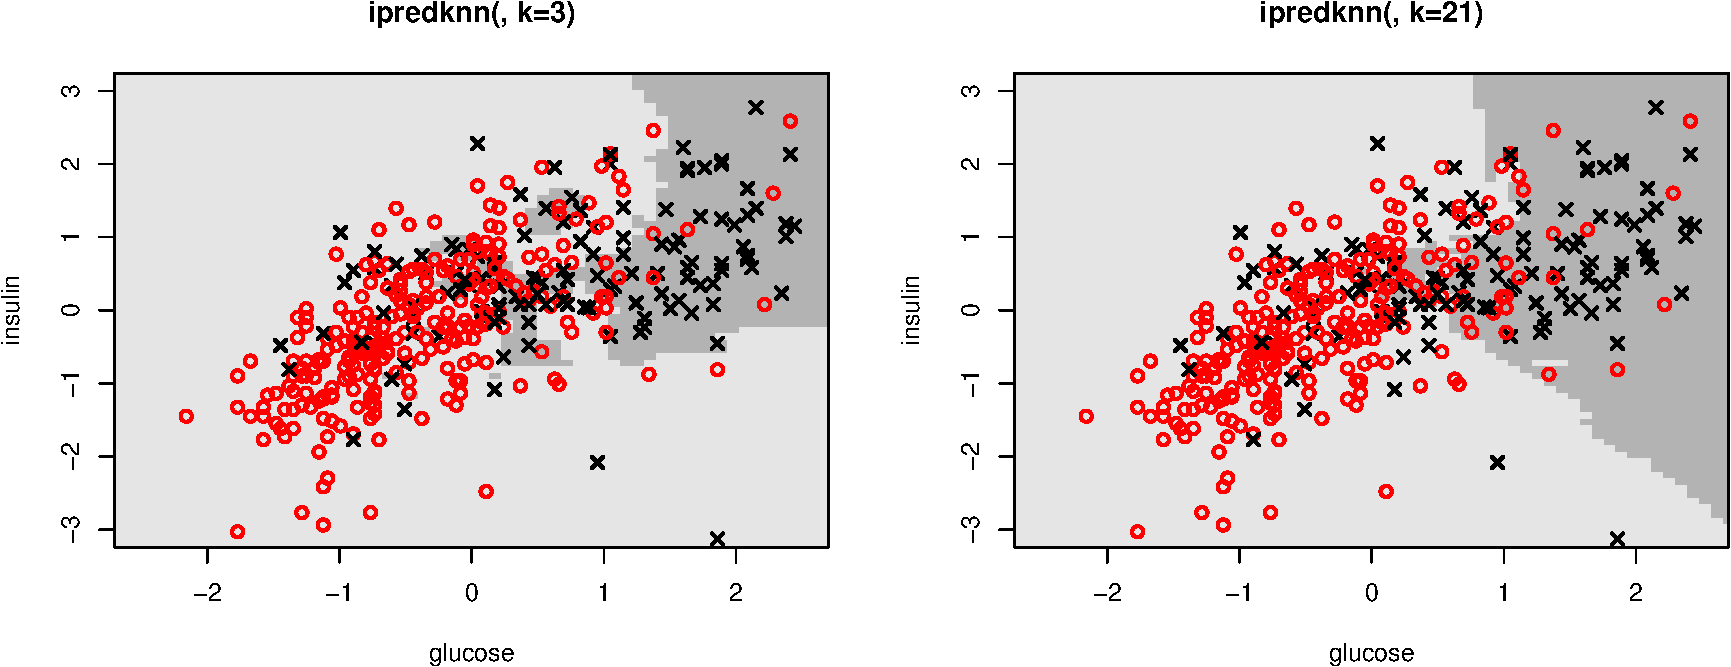
\includegraphics[width=1\linewidth]{NaPrzelajR_files/figure-latex/ad43-1} 

}

\caption{Przykładowe obszary decyzyjne dla metody k-sąsiadów z parametrami k=3 i k=21.}\label{fig:ad43}
\end{figure}

\hypertarget{part_43}{%
\section{Naiwny klasyfikator Bayesowski}\label{part_43}}

Do klasyfikacji wykorzystać można szeroką grupę metod bazujących na ocenie prawdopodobieństwa przynależności do określonej grupy. Dla każdej z klas ocenia się częstość (w przypadku ciągłym gęstość) występowania obiektów o określonych parametrach. Następnie dla nowego obiektu wyznacza się częstości występowania obiektów
poszczególnych klas i wybiera się klasę występującą dla tych parametrów najczęściej.

Do tej grupy metod należy naiwny klasyfikator Bayesowski. Bayesowski, ponieważ bazuje na regule Bayesa użytej do wyznaczenia prawdopodobieństwa a posteriori
należenia do poszczególnych klas. Naiwność w tym kontekście oznacza przyjęte założenie, że łączna gęstość występowania obiektów jest iloczynem gęstości brzegowych.
Naiwny klasyfikator Bayesowski jest dostępny w funkcjach \texttt{naiveBayes(e1071)} i \texttt{NaiveBayes(klaR)}.
Poniżej przedstawimy tą drugą implementację.
Sposób użycia tej funkcji jest podobny do użycia innych opisanych powyżej klasyfikatorów. Na rysunku \ref{fig:mN} przestawione są warunkowe brzegowe oceny gęstości dla
obu zmiennych dla każdej z klas, na bazie tych gęstości wykonywana jest kalsyfikacja. Na rysunku \ref{fig:NB} przedstawiamy przykładowe obszary decyzyjne dla naiwnego klasyfikatora Bayesowskiego.

\begin{Shaded}
\begin{Highlighting}[]
\CommentTok{# konstruujemy naiwny klasyfikator Bayesowski}
\NormalTok{mN <-}\StringTok{ }\NormalTok{klaR}\OperatorTok{::}\KeywordTok{NaiveBayes}\NormalTok{(diabetes}\OperatorTok{~}\NormalTok{glucose}\OperatorTok{+}\NormalTok{insulin, }\DataTypeTok{data=}\NormalTok{dane, }\DataTypeTok{subset=}\NormalTok{zbior.uczacy)}
\CommentTok{# wyznaczamy oceny}
\NormalTok{oceny <-}\StringTok{ }\KeywordTok{predict}\NormalTok{(mN, dane[}\OperatorTok{-}\NormalTok{zbior.uczacy,])}\OperatorTok{$}\NormalTok{class}
\KeywordTok{table}\NormalTok{(}\DataTypeTok{predykcja =}\NormalTok{ oceny, }\DataTypeTok{prawdziwe =}\NormalTok{ dane[}\OperatorTok{-}\NormalTok{zbior.uczacy,}\DecValTok{3}\NormalTok{])}
\end{Highlighting}
\end{Shaded}

\begin{verbatim}
##          prawdziwe
## predykcja neg pos
##       neg 112  24
##       pos  23  37
\end{verbatim}

\begin{Shaded}
\begin{Highlighting}[]
\KeywordTok{par}\NormalTok{(}\DataTypeTok{mfcol=}\KeywordTok{c}\NormalTok{(}\DecValTok{1}\NormalTok{,}\DecValTok{2}\NormalTok{))}
\KeywordTok{plot}\NormalTok{(mN)}
\end{Highlighting}
\end{Shaded}

\begin{figure}[h]

{\centering 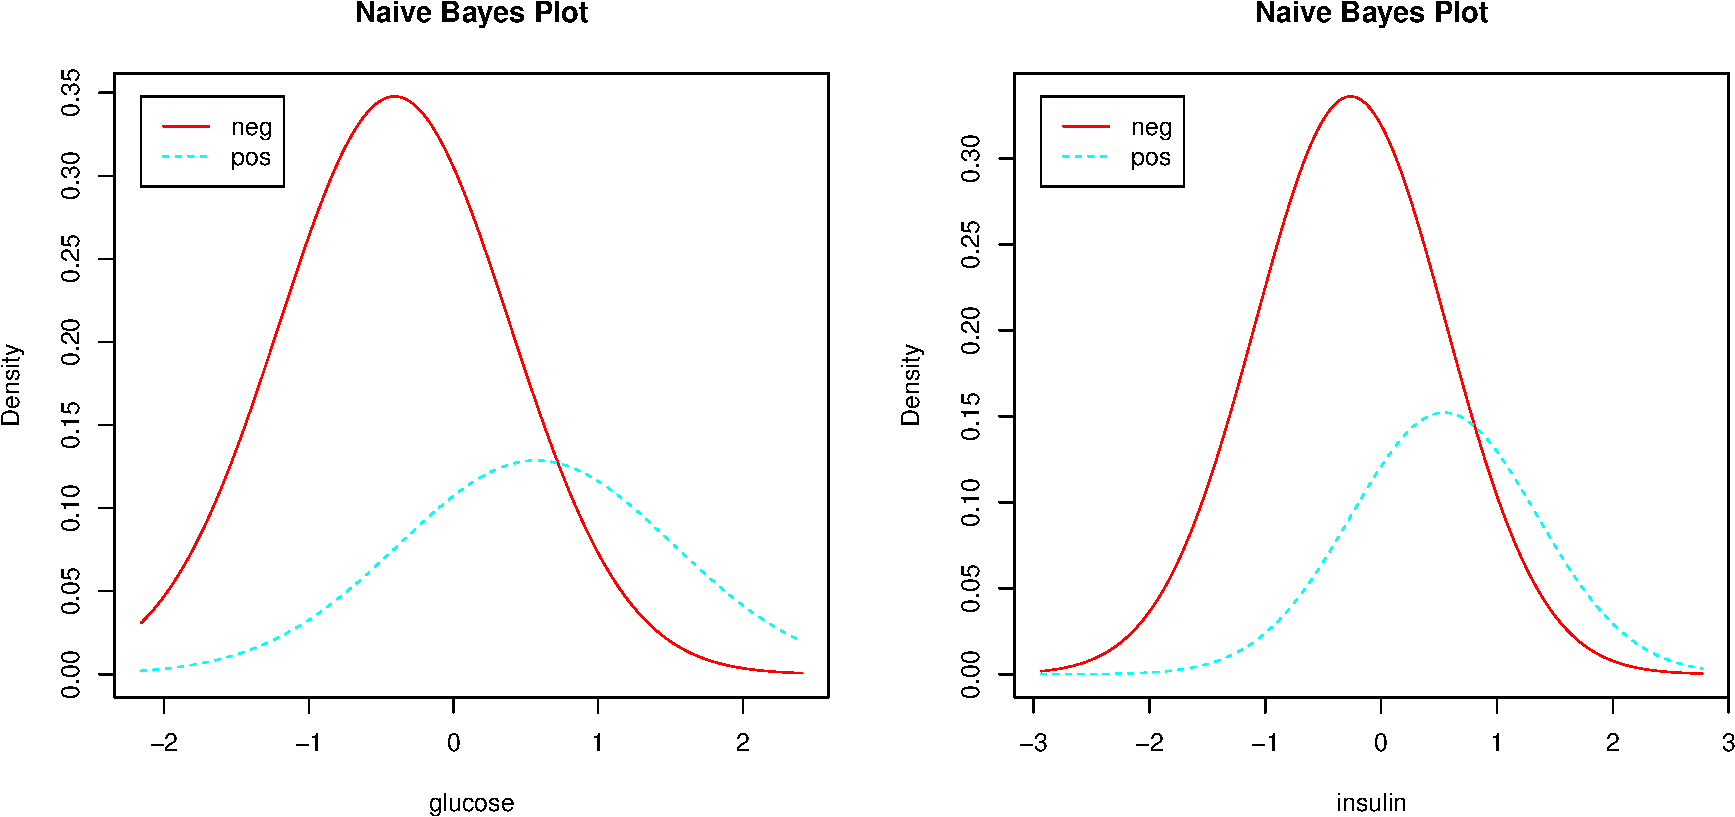
\includegraphics[width=0.7\linewidth]{NaPrzelajR_files/figure-latex/mN-1} 

}

\caption{Warunkowe brzegowe oceny gęstości, na ich bazie funkcjonuje naiwny klasyfikator Bayesowski.}\label{fig:mN}
\end{figure}

\begin{Shaded}
\begin{Highlighting}[]
\NormalTok{PimaIndiansDiabetes2 =}\StringTok{ }\KeywordTok{na.omit}\NormalTok{(PimaIndiansDiabetes2)}
\NormalTok{dane =}\StringTok{ }\NormalTok{PimaIndiansDiabetes2[,}\KeywordTok{c}\NormalTok{(}\DecValTok{2}\NormalTok{,}\DecValTok{5}\NormalTok{,}\DecValTok{9}\NormalTok{)]}
\NormalTok{dane[,}\DecValTok{2}\NormalTok{] =}\StringTok{ }\KeywordTok{log}\NormalTok{(dane[,}\DecValTok{2}\NormalTok{])}

\NormalTok{seqx =}\StringTok{ }\KeywordTok{seq}\NormalTok{(}\DecValTok{30}\NormalTok{,}\DecValTok{210}\NormalTok{,}\DecValTok{2}\NormalTok{)}
\NormalTok{seqy =}\StringTok{ }\KeywordTok{seq}\NormalTok{(}\FloatTok{2.5}\NormalTok{,}\DecValTok{7}\NormalTok{,}\FloatTok{0.07}\NormalTok{)}
\NormalTok{siata =}\StringTok{ }\KeywordTok{as.data.frame}\NormalTok{(}\KeywordTok{expand.grid}\NormalTok{(seqx, seqy))}

\NormalTok{kol  =}\StringTok{ }\KeywordTok{c}\NormalTok{(}\StringTok{"grey90"}\NormalTok{, }\StringTok{"grey70"}\NormalTok{)}
\NormalTok{klasyfikatorKNN =}\StringTok{ }\NormalTok{klaR}\OperatorTok{::}\KeywordTok{NaiveBayes}\NormalTok{(diabetes}\OperatorTok{~}\NormalTok{glucose}\OperatorTok{+}\NormalTok{insulin, }\DataTypeTok{data =}\NormalTok{ dane)}
\NormalTok{wub =}\StringTok{ }\KeywordTok{predict}\NormalTok{(klasyfikatorKNN, }\DataTypeTok{newdata=}\NormalTok{siata)}\OperatorTok{$}\NormalTok{class}
\KeywordTok{plot}\NormalTok{(siata, }\DataTypeTok{col=}\NormalTok{kol[}\KeywordTok{as.numeric}\NormalTok{(wub)], }\DataTypeTok{pch=}\DecValTok{15}\NormalTok{, }\DataTypeTok{main=}\StringTok{"NaiveBayes()"}\NormalTok{, }
     \DataTypeTok{xlab=}\StringTok{"insulin"}\NormalTok{,}\DataTypeTok{ylab=}\StringTok{"glucose"}\NormalTok{, }\DataTypeTok{xlim=}\KeywordTok{range}\NormalTok{(dat[,}\DecValTok{1}\NormalTok{]),}\DataTypeTok{ylim=}\KeywordTok{range}\NormalTok{(dat[,}\DecValTok{2}\NormalTok{]))}
\KeywordTok{points}\NormalTok{(dane[,}\DecValTok{1}\OperatorTok{:}\DecValTok{2}\NormalTok{],}\DataTypeTok{pch=}\KeywordTok{c}\NormalTok{(}\DecValTok{1}\NormalTok{,}\DecValTok{4}\NormalTok{)[}\KeywordTok{as.numeric}\NormalTok{(dane[,}\DecValTok{3}\NormalTok{])], }\DataTypeTok{cex=}\DecValTok{1}\NormalTok{, }
       \DataTypeTok{col=}\NormalTok{kol2[}\KeywordTok{as.numeric}\NormalTok{(dane[,}\DecValTok{3}\NormalTok{])], }\DataTypeTok{lwd=}\DecValTok{2}\NormalTok{)}
\end{Highlighting}
\end{Shaded}

\begin{figure}[h]

{\centering 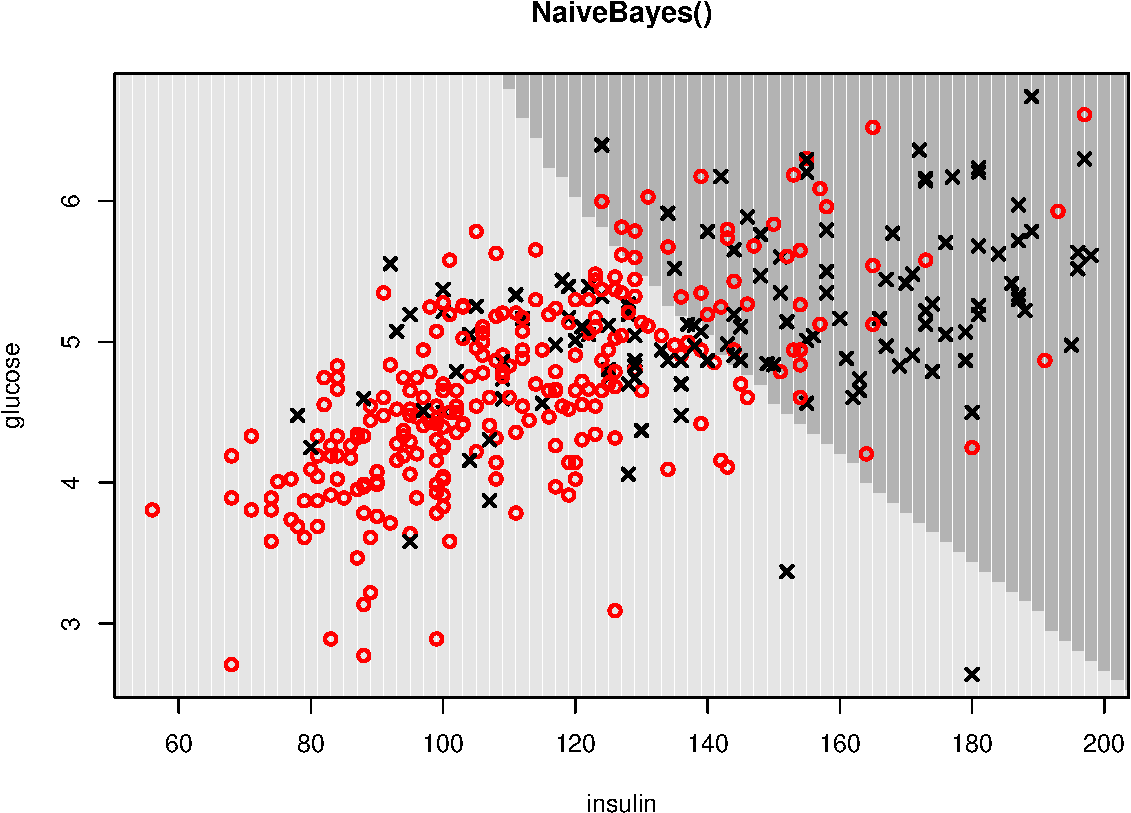
\includegraphics[width=0.7\linewidth]{NaPrzelajR_files/figure-latex/NB-1} 

}

\caption{Przykładowe obszary decyzyjne dla naiwnego klasyfikatora Bayesowskiego.}\label{fig:NB}
\end{figure}

\hypertarget{part_44}{%
\section{Drzewa decyzyjne}\label{part_44}}

Inną klasą klasyfikatorów są cieszące się dużą popularnością metody bazujące na
drzewach decyzyjnych (klasyfikacyjnych). W tym przypadku klasyfikator jest reprezentowany przez drzewo binarne, w którego węzłach znajdują się pytania o wartości
określonej cechy, a w liściach znajdują się oceny klas. Przykład drzewa klasyfikacyjnego przedstawiamy na rysunku \ref{fig:Ctree46}. Dodatkowo w liściach przedstawiono proporcję
obiektów z obu klas, które znalazły się w danym węźle, a wiec spełniły warunki
określone w poszczególnych węzłach drzewa. Jeżeli nowe obiekty będziemy przypisywać do klasy, która w danym liściu występowała najczęściej, to dla trzech liści
(czwartego, szóstego i siódmego) klasyfikować będziemy do grupy osób chorych, a w
pozostałych liściach będziemy klasyfikować do grupy osób zdrowych.

W pakiecie R metoda wyznaczania drzew decyzyjnych dostępna jest w wielu różnych funkcjach. Popularnie wykorzystywane są funkcje \texttt{tree(tree)}, \texttt{rpart(rpart)}
oraz \texttt{cpart(party)}. Poniżej przedstawimy tylko tą ostatnią, ponieważ są dla niej
opracowane najbardziej atrakcyjne funkcje do prezentacji graficznej. Z wszystkich
wymienionych funkcji do konstrukcji drzew korzysta się podobnie. Wymienione funkcje mogą służyć zarówno do wyznaczania drzew regresyjnych jak i klasyfikacyjnych, ale w tym miejscu przedstawimy tylko ich klasyfikacyjną naturę. Do wizualizacji drzew klasyfikacyjnych można wykorzystać (w zależności od tego jaką funkcją wyznaczyliśmy drzewo) funkcje \texttt{plot.BinaryTree(party)}, \texttt{plot.tree(tree)},
\texttt{text.tree(tree)}, \texttt{draw.tree(maptree)}, \texttt{plot.rpart(rpart)} oraz \texttt{text.rpart(rpart)}.

Aby zbudować drzewo klasyfikacyjne należy określić kryterium podziału, a więc
na jaka wartość ma być minimalizowana przy tworzeniu kolejnych gałęzi (najczęściej
jest to błąd klasyfikacji) oraz kryterium stopu (a wiec jak długo drzewo ma być dzielone). Różne warianty drzew umożliwiają kontrolę różnych kryteriów, w przypadku
metody \texttt{ctree()} zarówno kryterium stopu jak i podziału można określić argumentem \texttt{control} (patrz opis funkcji \texttt{ctree\_control(party)}). Poniżej przedstawiamy
przykładową sesję z budową drzewa klasyfikacyjnego.

\begin{Shaded}
\begin{Highlighting}[]
\CommentTok{# określamy kryteria budowy drzewa klasyfikayjnego}
\NormalTok{ustawienia <-}\StringTok{ }\NormalTok{party}\OperatorTok{::}\KeywordTok{ctree_control}\NormalTok{(}\DataTypeTok{mincriterion =} \FloatTok{0.5}\NormalTok{, }\DataTypeTok{testtype =} \StringTok{"Teststatistic"}\NormalTok{)}
\CommentTok{# uczymy drzewo}
\NormalTok{drzewo <-}\StringTok{ }\NormalTok{party}\OperatorTok{::}\KeywordTok{ctree}\NormalTok{(diabetes}\OperatorTok{~}\NormalTok{glucose}\OperatorTok{+}\NormalTok{insulin,}
                       \DataTypeTok{data=}\NormalTok{dane, }\DataTypeTok{subset =}\NormalTok{ zbior.uczacy, }\DataTypeTok{controls =}\NormalTok{ ustawienia)}
\CommentTok{# narysujmy je}
\KeywordTok{plot}\NormalTok{(drzewo)}
\end{Highlighting}
\end{Shaded}

\begin{figure}[h]

{\centering 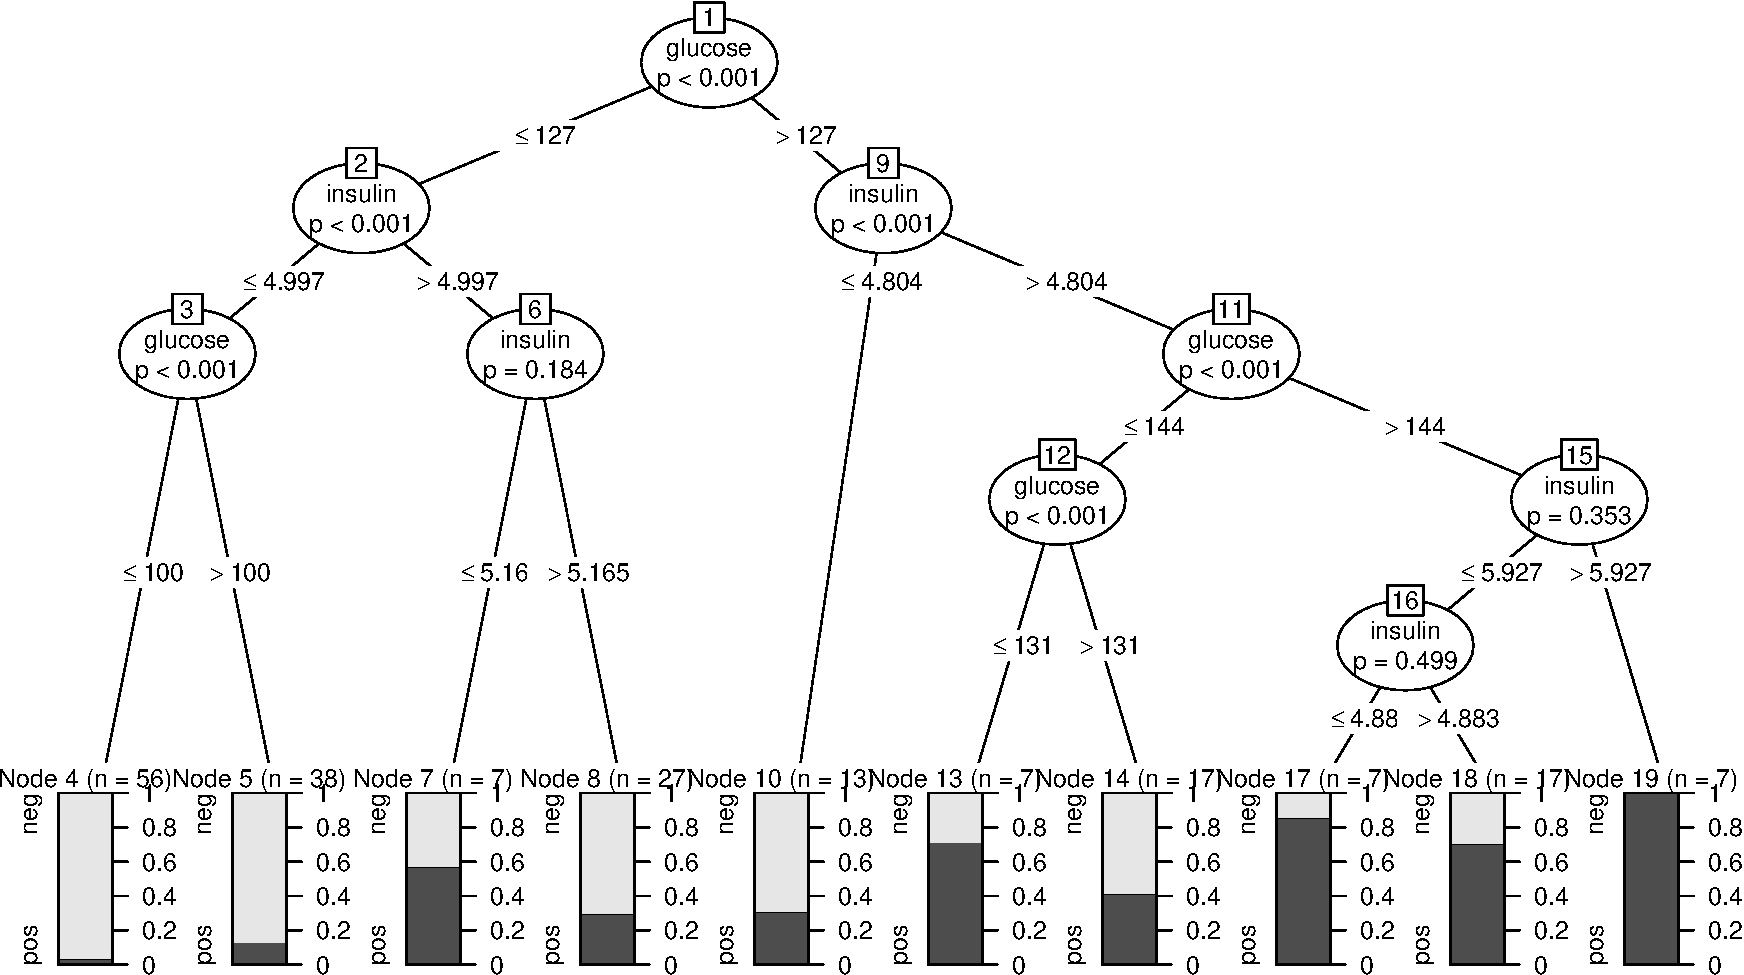
\includegraphics[width=0.8\linewidth]{NaPrzelajR_files/figure-latex/Ctree46-1} 

}

\caption{Przykładowe drzewo klasyfikacyjne wyznaczone funkcją ctree().}\label{fig:Ctree46}
\end{figure}

\begin{Shaded}
\begin{Highlighting}[]
\CommentTok{# w standardowy sposób przeprowadzamy klasyfikacje}
\NormalTok{oceny =}\StringTok{ }\KeywordTok{predict}\NormalTok{(drzewo, dane[}\OperatorTok{-}\NormalTok{zbior.uczacy,])}
\KeywordTok{table}\NormalTok{(}\DataTypeTok{predykcja =}\NormalTok{ oceny, }\DataTypeTok{prawdziwe =}\NormalTok{ dane[}\OperatorTok{-}\NormalTok{zbior.uczacy,}\DecValTok{3}\NormalTok{])}
\end{Highlighting}
\end{Shaded}

\begin{verbatim}
##          prawdziwe
## predykcja neg pos
##       neg 121  27
##       pos  14  34
\end{verbatim}

\begin{Shaded}
\begin{Highlighting}[]
\NormalTok{drzewo <-}\StringTok{ }\NormalTok{party}\OperatorTok{::}\KeywordTok{ctree}\NormalTok{(dane}\OperatorTok{$}\NormalTok{diabetes}\OperatorTok{~}\NormalTok{dane}\OperatorTok{$}\NormalTok{glucose}\OperatorTok{+}\NormalTok{dane}\OperatorTok{$}\NormalTok{insulin, }\DataTypeTok{data=}\NormalTok{dane,}
                       \DataTypeTok{controls =}\NormalTok{ party}\OperatorTok{::}\KeywordTok{ctree_control}\NormalTok{(}
                         \DataTypeTok{mincriterion =} \FloatTok{0.5}\NormalTok{, }\DataTypeTok{teststat =} \KeywordTok{c}\NormalTok{(}\StringTok{"max"}\NormalTok{)))}
\NormalTok{wub =}\StringTok{ }\KeywordTok{predict}\NormalTok{(drzewo, siata)}
\KeywordTok{plot}\NormalTok{(siata, }\DataTypeTok{col=}\NormalTok{kol[}\KeywordTok{as.numeric}\NormalTok{(wub)], }\DataTypeTok{pch=}\DecValTok{15}\NormalTok{, }\DataTypeTok{main=}\StringTok{"ctree()"}\NormalTok{,}
     \DataTypeTok{xlab=}\StringTok{"insulin"}\NormalTok{,}\DataTypeTok{ylab=}\StringTok{"glucose"}\NormalTok{, }\DataTypeTok{xlim=}\KeywordTok{range}\NormalTok{(dat[,}\DecValTok{1}\NormalTok{]),}\DataTypeTok{ylim=}\KeywordTok{range}\NormalTok{(dat[,}\DecValTok{2}\NormalTok{]))}
\KeywordTok{points}\NormalTok{(dane[,}\DecValTok{1}\OperatorTok{:}\DecValTok{2}\NormalTok{],}\DataTypeTok{pch=}\KeywordTok{c}\NormalTok{(}\DecValTok{1}\NormalTok{,}\DecValTok{4}\NormalTok{)[}\KeywordTok{as.numeric}\NormalTok{(dane[,}\DecValTok{3}\NormalTok{])], }\DataTypeTok{cex=}\DecValTok{1}\NormalTok{,}
       \DataTypeTok{col=}\NormalTok{kol2[}\KeywordTok{as.numeric}\NormalTok{(dane[,}\DecValTok{3}\NormalTok{])], }\DataTypeTok{lwd=}\DecValTok{2}\NormalTok{)}
\end{Highlighting}
\end{Shaded}

\begin{figure}[h]

{\centering 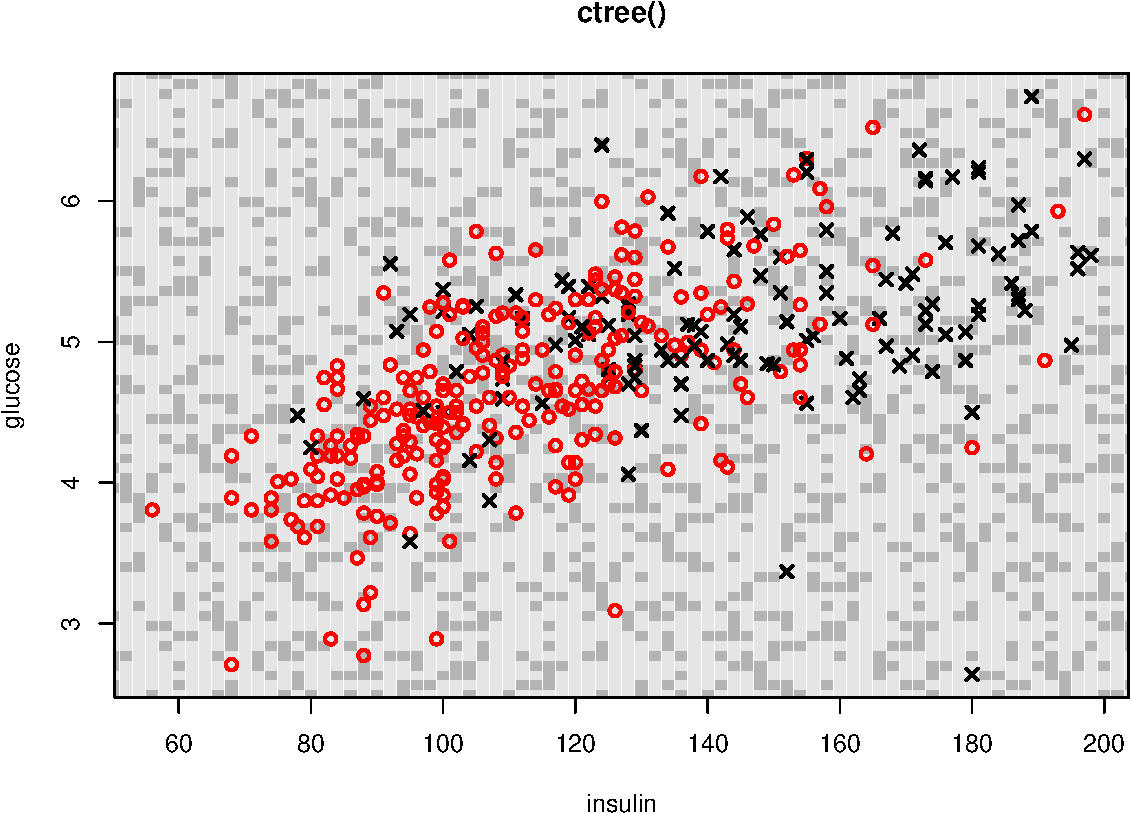
\includegraphics[width=0.7\linewidth]{NaPrzelajR_files/figure-latex/Ktree47-1} 

}

\caption{Przykładowe obszary decyzyjne dla drzewa klasyfikacyjnego.}\label{fig:Ktree47}
\end{figure}

Zaletą drzew jest ich łatwość w interpretacji. Narysowany klasyfikator może być
oceniony i poprawiony, przez eksperta z dziedziny, której problem dotyczy.

Dla drzew zapisanych jako obiekty klasy \texttt{tree} lub \texttt{rpart} dostępne są dwie przydatne funkcje umożliwiające modyfikację drzewa. Pierwsza to \texttt{prune.tree(tree)}
(\texttt{prune.rpart(rpart)}). Pozwala ona na automatyczne przycinanie drzewa, poszczególnymi argumentami tej funkcji możemy ustalić jak drzewo ma być przycięte. Można określić pożądaną liczbę węzłów w drzewie, maksymalny współczynnik błędu
w liściu drzewa oraz inne kryteria. Nie zawsze przycinanie automatyczne daje satysfakcjonujące rezultaty. W sytuacji gdy drzewo potrzebuje ludzkiej ingerencji można wykorzystać funkcję \texttt{snip.tree(tree)} (\texttt{snip.rpart(rpart)}) pozwalającą użytkownikowi na wskazanie myszką które węzły drzewa maja być usunięte. Inne ciekawe funkcje to \texttt{misclass.tree(tree)} (wyznacza błąd klasyfikacji dla każdego węzła z drzewa) oraz \texttt{partition.tree(tree)} (wyznacza obszary decyzyjne dla drzew).

\hypertarget{part_45}{%
\section{Lasy losowe}\label{part_45}}

Wadą drzew klasyfikacyjnych jest ich mała stabilność. Są jednak sposoby by temu
zaradzić. Takim sposobem jest konstruowanie komitetu klasyfikatorów a wiec użycie
metody bagging lub boosting. Nie wystarczyło tu miejsca by przedstawić te metody
w ich ogólnej postaci, wspomnimy o nich na przykładzie lasów losowych.

Idea, która przyświeca metodzie lasów losowych możne być streszczona w zdaniu
``Niech lasy składają się z drzew''. Jak pamiętamy w metodzie bootstrap generowano
replikacje danych, by ocenić zachowanie statystyki dla oryginalnego zbioru danych.
Odmianą metody bootstrap w zagadnieniu klasyfikacji jest bagging. Na bazie replikacji zbioru danych konstruowane są klasyfikatory, które na drodze głosowania
większością wyznaczają ostateczną klasą dla danej obserwacji. W przypadku lasów
losowych komitet klasyfikatorów składa się z drzew klasyfikacyjnych, które są trenowane na replikacjach zbioru danych, dla ustalonego podzbioru zmiennych.

Ponieważ drzew w lesie jest dużo, do komitet głosujący demokratycznie charakteryzuje się większą stabilnością. Dodatkową zaletą drzew jest naturalny nieobciążony
estymator błędu klasyfikacji. Generując replikacje losując metodą z powtórzeniami,
średnio do replikacji nie trafia około jednej trzeciej obserwacji (w ramach ćwiczeń
warto to sprawdzić). Te obserwacje, które nie trafiły do replikacji, można wykorzystać do oceny klasyfikatora nauczonego na danej replikacji. Taka ocena błędu określana jest błędem OOB (ang. out-of-bag). Jeszcze inną zaletą drzew losowych jest
możliwość oceny zdolności dyskryminujących dla poszczególnych zmiennych (dzięki
czemu możemy wybrać najlepszy zbiór zmiennych).

Lasy losowe dostępne są w funkcji \texttt{randomForest(randomForest)}. Poniżej przedstawiamy przykład jej użycia. Ponieważ przy konstrukcji lasów losowych generowane
są losowe replikacje zbioru danych, to aby móc odtworzyć uzyskane wyniki warto
skorzystać z funkcji \texttt{set.seed()}.

\begin{Shaded}
\begin{Highlighting}[]
\CommentTok{# ustawiamy ziarno generatora, by można było odtworzyć te wyniki}
\KeywordTok{set.seed}\NormalTok{(}\DecValTok{1}\NormalTok{)}

\CommentTok{# ćwiczymy las}
\NormalTok{klasyfikatorRF <-}\StringTok{ }\NormalTok{randomForest}\OperatorTok{::}\KeywordTok{randomForest}\NormalTok{(diabetes}\OperatorTok{~}\NormalTok{glucose}\OperatorTok{+}\NormalTok{insulin,}
                                             \DataTypeTok{data=}\NormalTok{dane,}
                                             \DataTypeTok{subset=}\NormalTok{zbior.uczacy, }\DataTypeTok{importance=}\OtherTok{TRUE}\NormalTok{, }\DataTypeTok{proximity=}\OtherTok{TRUE}\NormalTok{)}
\CommentTok{# podsumowanie lasu}
\KeywordTok{print}\NormalTok{(klasyfikatorRF)}
\end{Highlighting}
\end{Shaded}

\begin{verbatim}
## 
## Call:
##  randomForest(formula = diabetes ~ glucose + insulin, data = dane,      importance = TRUE, proximity = TRUE, subset = zbior.uczacy) 
##                Type of random forest: classification
##                      Number of trees: 500
## No. of variables tried at each split: 1
## 
##         OOB estimate of  error rate: 29.08%
## Confusion matrix:
##     neg pos class.error
## neg 105  22   0.1732283
## pos  35  34   0.5072464
\end{verbatim}

\begin{Shaded}
\begin{Highlighting}[]
\CommentTok{# podobnie jak dla innych klasyfikatorów funkcją predict() możemy ocenić}
\CommentTok{# etykietki na zbiorze testowym i porównać błąd klasyfikacji z błędem z}
\CommentTok{# innych metod}
\NormalTok{oceny =}\StringTok{ }\KeywordTok{predict}\NormalTok{(klasyfikatorRF, dane[}\OperatorTok{-}\NormalTok{zbior.uczacy,])}
\KeywordTok{table}\NormalTok{(}\DataTypeTok{predykcja =}\NormalTok{ oceny, }\DataTypeTok{prawdziwe =}\NormalTok{ dane[}\OperatorTok{-}\NormalTok{zbior.uczacy,}\StringTok{"diabetes"}\NormalTok{])}
\end{Highlighting}
\end{Shaded}

\begin{verbatim}
##          prawdziwe
## predykcja neg pos
##       neg 114  29
##       pos  21  32
\end{verbatim}

\begin{Shaded}
\begin{Highlighting}[]
\NormalTok{PimaIndiansDiabetes2 =}\StringTok{ }\KeywordTok{na.omit}\NormalTok{(PimaIndiansDiabetes2)}
\NormalTok{dane =}\StringTok{ }\NormalTok{PimaIndiansDiabetes2}
\NormalTok{dane[,}\DecValTok{5}\NormalTok{] =}\StringTok{ }\KeywordTok{log}\NormalTok{(dane[,}\DecValTok{5}\NormalTok{])}

\NormalTok{seqx =}\StringTok{ }\KeywordTok{seq}\NormalTok{(}\DecValTok{30}\NormalTok{,}\DecValTok{210}\NormalTok{,}\DecValTok{2}\NormalTok{)}
\NormalTok{seqy =}\StringTok{ }\KeywordTok{seq}\NormalTok{(}\DecValTok{2}\NormalTok{,}\DecValTok{7}\NormalTok{,}\FloatTok{0.07}\NormalTok{)}
\NormalTok{siata =}\StringTok{ }\KeywordTok{as.data.frame}\NormalTok{(}\KeywordTok{expand.grid}\NormalTok{(seqx, seqy))}
\KeywordTok{colnames}\NormalTok{(siata) =}\StringTok{ }\KeywordTok{c}\NormalTok{(}\StringTok{"glucose"}\NormalTok{, }\StringTok{"insulin"}\NormalTok{)}

\NormalTok{klasyfikatorRF <-}\StringTok{ }\NormalTok{randomForest}\OperatorTok{::}\KeywordTok{randomForest}\NormalTok{(diabetes}\OperatorTok{~}\NormalTok{glucose}\OperatorTok{+}\NormalTok{insulin,}
                                             \DataTypeTok{data=}\NormalTok{dane,}\DataTypeTok{importance=}\OtherTok{TRUE}\NormalTok{, }\DataTypeTok{proximity=}\OtherTok{TRUE}\NormalTok{)}
\CommentTok{#klasyfikatorRF <- randomForest(diabetes~., data=dane,importance=TRUE, proximity=TRUE)}
\NormalTok{wub =}\StringTok{ }\KeywordTok{predict}\NormalTok{(klasyfikatorRF, siata)}
\KeywordTok{plot}\NormalTok{(siata, }\DataTypeTok{col=}\NormalTok{kol[}\KeywordTok{as.numeric}\NormalTok{(wub)], }\DataTypeTok{pch=}\DecValTok{15}\NormalTok{, }
     \DataTypeTok{main=}\StringTok{"randomForest()"}\NormalTok{,}\DataTypeTok{xlim=}\KeywordTok{range}\NormalTok{(dane[,}\StringTok{"glucose"}\NormalTok{]),}\DataTypeTok{ylim=}\KeywordTok{range}\NormalTok{(dane[,}\StringTok{"insulin"}\NormalTok{]),}
     \DataTypeTok{cex=}\DecValTok{1}\NormalTok{)}
\KeywordTok{points}\NormalTok{(dane[,}\KeywordTok{c}\NormalTok{(}\StringTok{"glucose"}\NormalTok{,}\StringTok{"insulin"}\NormalTok{)],}\DataTypeTok{pch=}\KeywordTok{c}\NormalTok{(}\DecValTok{1}\NormalTok{,}\DecValTok{4}\NormalTok{)[}\KeywordTok{as.numeric}\NormalTok{(dane[,}\StringTok{"diabetes"}\NormalTok{])], }
       \DataTypeTok{cex=}\DecValTok{1}\NormalTok{, }\DataTypeTok{col=}\NormalTok{kol2[}\KeywordTok{as.numeric}\NormalTok{(dane[,}\StringTok{"diabetes"}\NormalTok{])], }\DataTypeTok{lwd=}\DecValTok{2}\NormalTok{)}
\end{Highlighting}
\end{Shaded}

\begin{figure}[h]

{\centering 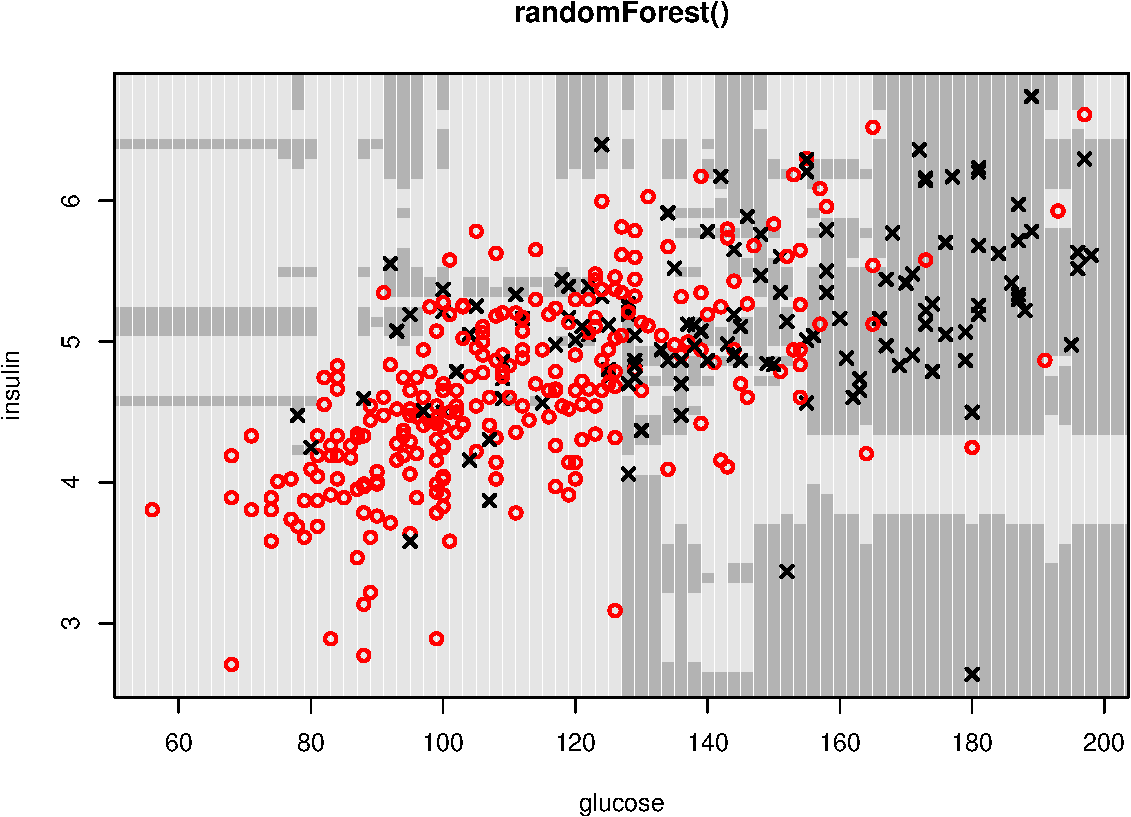
\includegraphics[width=0.7\linewidth]{NaPrzelajR_files/figure-latex/RF48-1} 

}

\caption{Przykładowe obszary decyzyjne dla lasów losowych.}\label{fig:RF48}
\end{figure}

Lasy losowe są uznawane za jedną z najlepszych metod klasyfikacji. Ich dodatkową zaletą jest możliwość użycia nauczonego lasu losowego do innych zagadnień niż
tylko do klasyfikacji. Przykładowo na podstawie drzew z lasu można wyznaczyć ranking zmiennych, a tym samym określić które zmienne mają lepsze właściwości predykcyjne a które gorsze. Taką informację przekazuje funkcja \texttt{importance(randomForest)},
można tę informacje również przedstawić graficznie z użyciem funkcji \texttt{varImpPlot(randomForest)}
(przykład dla naszego zbioru danych jest przedstawiony na rysunku \ref{fig:kl49}).

Używając lasów losowych (regresyjnych) można również wykonać imputacje,
a wiec zastąpić brakujące obserwacje w zbiorze danych. Do tego celu można posłużyć się funkcją \texttt{rfImpute(randomForest)}. Można również zdefiniować na podstawie
lasów losowych miarę odstępstwa i wykrywać nią obserwacje odstające (do tego celu służy funkcja \texttt{outlier(randomForest)}). Można rónież używając lasów losowych
przeprowadzać skalowanie wielowymiarowe, osoby zainteresowane tym tematem powinny zaznajomić się z funkcją \texttt{MDSplot(randomForest)}

\begin{Shaded}
\begin{Highlighting}[]
\NormalTok{klasyfikatorRF <-}\StringTok{ }\NormalTok{randomForest}\OperatorTok{::}\KeywordTok{randomForest}\NormalTok{(diabetes}\OperatorTok{~}\StringTok{ }\NormalTok{.,}
                                             \DataTypeTok{data=}\NormalTok{PimaIndiansDiabetes2,}
                                             \DataTypeTok{importance=}\OtherTok{TRUE}\NormalTok{,}\DataTypeTok{proximity=}\OtherTok{TRUE}\NormalTok{)}
\NormalTok{randomForest}\OperatorTok{::}\KeywordTok{varImpPlot}\NormalTok{(klasyfikatorRF)}
\end{Highlighting}
\end{Shaded}

\begin{figure}[h]

{\centering 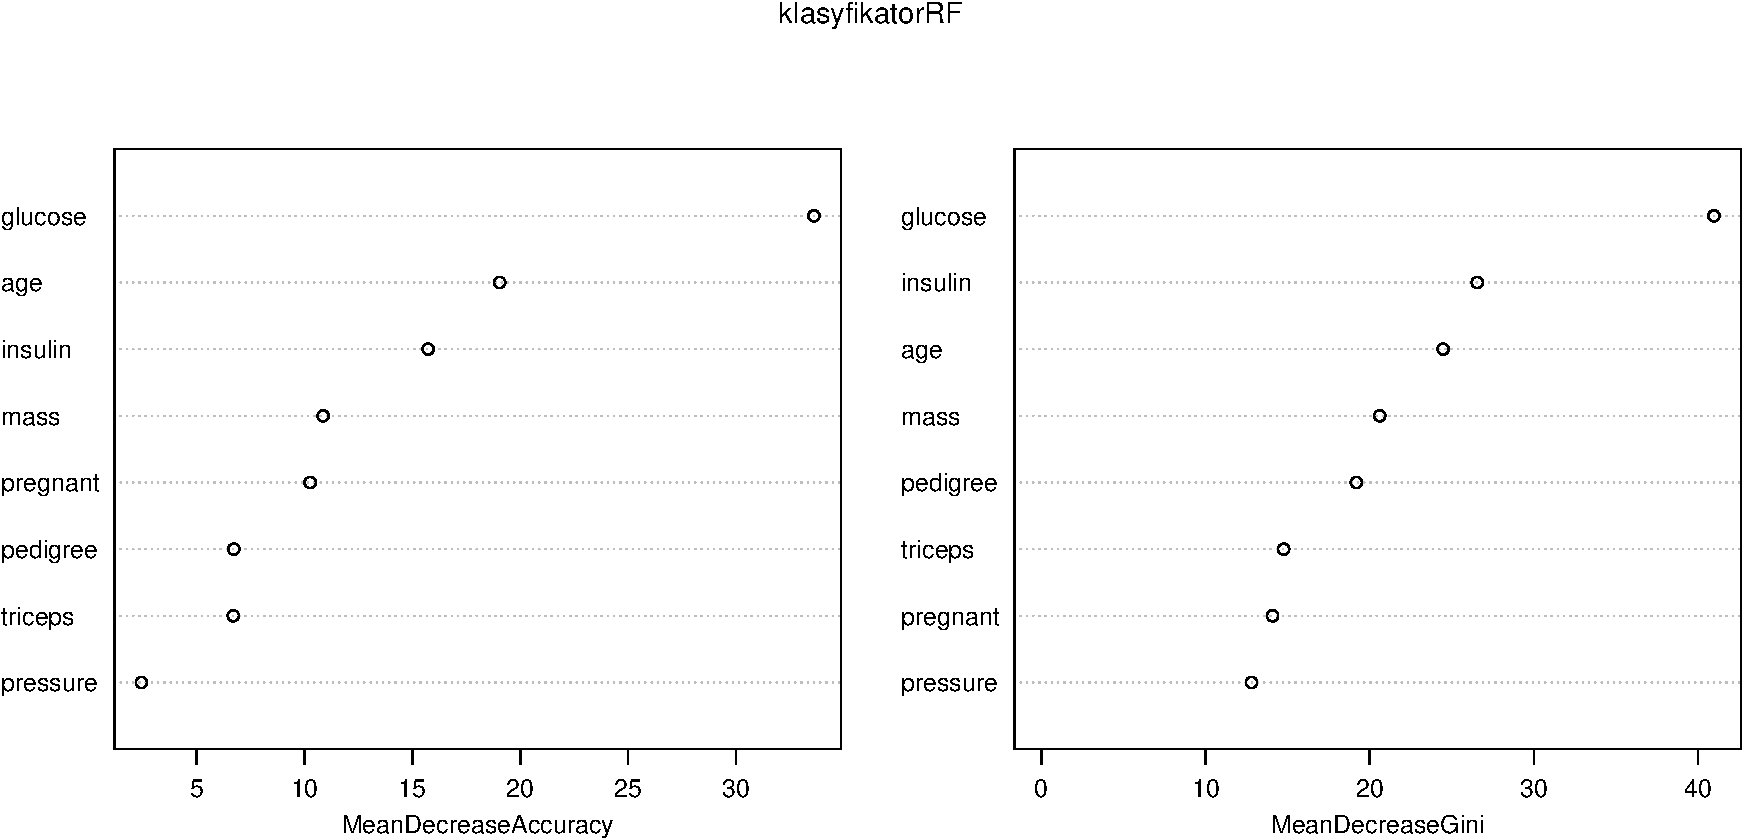
\includegraphics[width=0.7\linewidth]{NaPrzelajR_files/figure-latex/kl49-1} 

}

\caption{Ranking zmiennych wykonany przez las losowy.}\label{fig:kl49}
\end{figure}

\hypertarget{part_46}{%
\section{Inne klasyfikatory}\label{part_46}}

Powyżej wymienione metody to zaledwie początek góry lodowej funkcji do klasyfikacji dostępnych w pakiecie R. Poniżej wymienimy jeszcze kilka nazw popularnych
klasyfikatorów, oraz pokażemy w których funkcjach i pakietach dane metody są dostępne.

\begin{itemize}
\item
  \textbf{Sieci neuronowe}.
  Sieci neuronowe gotowe do użycia w zagadnieniach klasyfikacji są dostępne
  w funkcjach \texttt{nnet(nnet)} (prosta w użyciu sieć z jedną warstwą neuronów
  ukrytych) i \texttt{train(AMORE)} (bardziej zaawansowana funkcja do uczenia sieci
  neuronowych).
\item
  \textbf{Metoda wektorów podpierających (SVM, ang. Support Vector Machines)}.
  Ideą wykorzystywaną w tej technice jest zwiększenie wymiaru przestrzeni obserwacji (przez dodanie nowych zmiennych np. transformacji zmiennych oryginalnych) tak by obiekty różnych klas można było rozdzielić hiperpłaszczyznami. Ta technika zyskała wielu zwolenników, funkcje pozwalające na jej wykorzystanie znajdują się w kilku pakietach np. \texttt{ksvm(kernlab)}, \texttt{svm(1071)},
  \texttt{svmlight(klaR)}, \texttt{svmpath(svmpath)}.
\item
  \textbf{Nearest mean classification i Nearest Shrunken Centroid Classifier}.
  Zasady działania podobne jak dla metod analizy skupień k-średnich i PAM.
  Metoda Nearest mean classification dostępna w funkcji \texttt{nm(klaR)} wyznacza
  średnie dla obiektów z danej klasy i nowe obiekty klasyfikuje do poszczególnych klas na podstawie wartości odległości nowej obserwacji od wyznaczonych
  średnich. Metoda Nearest Shrunken Centroid Classifier dostępna w funkcji
  \texttt{pamr.train(pamr)} działa podobnie, tyle, że zamiast średnich wyznacza centroidy.
\item
  \textbf{Metody bagging i boosting}.
  Idea obu metod opiera się na tworzeniu replikacji zbioru danych, na których
  uczone są klasyfikatory. Wiele funkcji ze wsparciem dla tych metod znajduje się
  w pakiecie \texttt{boost} (boosting) i \texttt{ipred} (bagging), np. funkcje \texttt{adaboost(boost)},
  \texttt{bagboost(boost)}, \texttt{l2boost(boost)}, \texttt{logitboost(boost)}, \texttt{ipredbagg(ipred)}.
\end{itemize}

\hypertarget{part_5}{%
\chapter{Analiza kanoniczna}\label{part_5}}

Podstawowe problemy i wyniki analizy kanonicznej zostały sformułowane przez Harolda Hotellinga (wybitny ekonomista, matematyk, statystyk) w latach 1935-36.
Powstała jako metoda do badania zależności pomiędzy dwoma zbiorami zmiennych.
Do dziś doczekała się wielu uogólnień i rozszerzeń, np. na badanie relacji pomiędzy wieloma zbiorami zmiennych, na badane relacji w obecności współliniowych
zmiennych (przez regularyzację) itp.

\hypertarget{part_51}{%
\section{Problem}\label{part_51}}

Mamy dwa zbiory zmiennych \(\{X_1,\dots,X_p\}\) i \(\{Y_1\dots,Y_p\}\).

Chcemy znaleźć taką kombinację liniową zmiennych z pierwszego zbioru, aby
korelowała ona możliwie najsilniej ze zmiennymi z drugiego zbioru.

Innymi słowy, szukamy wektorów współczynników \(a\) i \(b\), takich, że
\[cor(a^{\prime}X,b^{\prime}Y)\]
jest możliwie największa.

\hypertarget{part_52}{%
\section{Rozwiązanie}\label{part_52}}

Wektor współczynników a to wektor własny odpowiadający największej wartości
własnej macierzy
\[S^{-1}_{22}S_{21}S^{-1}_{11}S_{12}\]
a wektor współczynników b to wektor własny odpowiadający największej wartości
własnej macierzy
\[S^{-1}_{11}S_{12}S^{-1}_{22}S_{21}\]
Korelacja \(cor(a^{\prime}X,b^{\prime}Y)\) to wartość największa wartość własna z powyższych macierzy.

{[}Wyprowadzenie na tablicy{]}

Nowe zmienne \(u_1=a^{\prime}X\) i \(v_1=b^{\prime}Y\) wyjaśniają największą część korelacji pomiędzy zbiorami wektorów \(X\) i \(Y\), ale nie całą.

Kolejnym krokiem jest znalezienie kolejnych zmiennych \(u_i=a_{i}X\) i \(u_i=b_iY\) , tak by:

\begin{itemize}
\item
  wektory \(u_i\) są nieskorelowane pomiędzy sobą,
\item
  wektory \(v_i\) są nieskorelowane pomiędzy sobą,
\item
  korelacje \(cor(u_i,v_i)\) tworzą nierosnący ciąg odpowiadający możliwie największym cząstkowym korelacjom.
\end{itemize}

Jeżeli obserwacje pochodzą z wielowymiarowego modelu normalnego \(N(\mu,\sum)\) to
możemy testować:
\[H_0:R_i=0\forall_i\]
Statystyka testowa dla testu ilorazu wiarogodności
\[LRT=-n\sum_{i=k+1}^{s}\log(1-R^2_i)\]
ma asymptotyczny rozkład \(\chi^2_{(p-k)(q-k)}\).

Wartość \(n\) w statystykach testowych zamienia się czasem na \(n - \frac{1}{2} (p + q + 3)\), co poprawia test.

\hypertarget{part_53}{%
\section{Założenia}\label{part_53}}

\begin{itemize}
\item
  wielowymiarowa normalność,
\item
  brak obserwacji odstających (miara Cooka, Leverage, test Grubbsa, test Dixona)
\item
  brak współliniowości (reguła kciuka, wyznacznik \(>10^{-5}\) )
\end{itemize}

Liczba obserwacji powinna być większa od około 20*liczba zmiennych.

\hypertarget{part_54}{%
\section{Jak to zrobić w R}\label{part_54}}

Analiza kanoniczna jest zaimplementowana między innymi w pakiecie \texttt{CCA} w funkcji \texttt{cc()}.

Prześledźmy poniższy kod

\begin{verbatim}
> library(CCA)
> dane = read.table("dane.csv",header=T,sep=";")
> X = dane[,c(9:10)]
# kolumny z waga
> Y = dane[,c(11:17)]
# kolumny z MDRD
> wynik = cc(X,Y)
> wynik$cor
[1] 0.3754946 0.1907164
\end{verbatim}

\begin{verbatim}
> wynik$xcoef
[,1]
[,2]
wagastart 0.1047822 -0.09276486
wagaend
-0.1154909 0.01404359
> wynik$ycoef
[,1]
[,2]
MDRD7
0.056059823 0.05799373
MDRD30 -0.059196976 -0.03981322
MDRD6m -0.006987328 0.02870234
MDRD12m -0.094082377 0.07732582
MDRD24m 0.119735985 -0.09688825
MDRD36m -0.024980200 -0.01744831
MDRD60m -0.007345604 0.04083270
> plot(wynik$cor,type="b")
> plt.cc(wynik,var.label=T)
\end{verbatim}

\hypertarget{part_55}{%
\section{Przykładowe wyniki}\label{part_55}}

\begin{figure}

{\centering \includegraphics[width=1\linewidth]{w1} 

}

\caption{w1}\label{fig:w1}
\end{figure}
\begin{figure}

{\centering \includegraphics[width=1\linewidth]{w2} 

}

\caption{w2}\label{fig:w2}
\end{figure}

\hypertarget{part_56}{%
\section{Studium przypadku}\label{part_56}}

\hypertarget{part_6}{%
\chapter{Analiza korespondencji (odpowiedniości)}\label{part_6}}

\hypertarget{part_61}{%
\section{Problem}\label{part_61}}

Obserwujemy dwie zmienne jakościowe. Pierwsza zmienna przyjmuje wartości z \(n_1\)
poziomów, druga z \(n_2\) poziomów.

Interesuje nas, czy zmienne te są od siebie niezależne, a jeżeli nie są niezależne
to które kombinacje poziomów występują ze sobą znacznie częściej.
Dane z którymi mamy do czynienia to macierz kontyngencji (tabela wielodziel-
cza) o wymiarach k × l wyznaczona dla dwóch zmiennych o odpowiednio \(k\) i \(l\) poziomach. Jeżeli \(k\) i \(l\) są małe, to taką macierz można ogarnąć rzutem oka. Jednak dla zmiennych występujących na wielu poziomach potrzebne są już dodatkowe narzędzia.

\hypertarget{part_62}{%
\section{Rozwiązanie}\label{part_62}}

Aby ocenić niezależność dwóch zmiennych można wykorzystać test \(\chi^2\) z funkcji
\href{https://rdrr.io/r/stats/chisq.test.html}{\texttt{chisq.test()}} lub inny test dla macierzy kontyngencji (jeżeli poziomy są uporządkowane to dobrym rozwiązaniem będzie test Cochrana-Armitage). Testem tym zweryfikujemy hipotezę o niezależności częstości występowań poszczególnych zmiennych.
Jeżeli jednak odrzucimy tę hipotezę zerową, czyli przyjmiemy że jest JAKAŚ
zależność, to naturalnym pytaniem będzie jaka to zależność i pomiędzy którymi
poziomami.
Aby ocenić, które zmienne występują częściej ze sobą można wykonuje się tzw.
analizę korespondencji. Jeżeli zmienne były by niezależne od siebie, to zachodziło
by równanie
\[
p_{ij}=p_{i\cdot}p_{\cdot j},\quad i\in \{1\dots k\},\quad j\in \{1\dots l\}.
\]
gdzie \(p_{ij}\) to prawdopodobieństwo zaobserwowania pierwszej zmiennej na poziomie
\(i\) i jednocześnie drugiej na poziomie \(j\), \(p_{i\cdot}\) to prawdopodobieństwo zaobserwowania zmiennej pierwszej na poziomie \(i\) a \(p_{\cdot j}\) to prawdopodobieństwo zaobserwowania zmiennej drugiej na poziomie \(j\).

Żeby ocenić, które zmienne występują częściej lub rzadziej niż wynikało by to
z niezależności, wyznaczymy standaryzowane reszty Pearsonowskie, zastąpimy też
prawdopodobieństwa ich częstościowymi ocenami (czyli \(\hat{p}\)
to liczba obserwowanych
zdarzeń podzielona przez liczbę wszystkich obserwowanych zdarzeń)
\[
\hat{e}_{ij}=\frac{\hat{p}_{ij}-\hat{p}_{i\cdot}\hat{p}_{\cdot j}}{\hat{p}_{i\cdot}\hat{p}_{\cdot j}}
\]
Duże dodatnie wartości \(\hat{e}_{ij}\) odpowiadają wysokiemu współwystępowaniu, ujemne \(E=[\hat{e}_{ij}]\) przedstawić w postaci graficznej używając tzw. biplotu. Innymi słowy wyznaczamy dekompozycję SVD macierzy E
wartości odpowiadają występowaniu rzadszemu niż losowe. Możemy teraz macierz
\[
E_{k\times l}=U_{k\times k}\sum_{k\times k}V_{l \times l}^{T}
\]

Kolumny macierzy \(U_{k \times k}\) to wektory własne macierzy \(E^T E\) a kolumny macierzy \(V\)
to wektory własne macierzy \(EE^T\). Na przekątnej macierzy diagonalnej \(\sigma\) znajdują
się tzw. wartości singularne (osobliwe?) równe pierwiastkom z wartości własnych
macierzy \(E^TE\) i EE\^{}T . ``Przy okazji''" kolumny macierzy \(U\) rozpinają ortonormalną
bazę na kolumnach macierzy \(E\) a kolumny macierzy \(V\) rozpinają ortonormlaną bazę
na wierszach macierzy \(E\). Można więc przedstawić macierz \(E\) (lub możliwie dużo
informacji z tej macierzy) we nowej przestrzeni określonej na bazie współrzędnych
wierszy i kolumn macierzy \(E\).

\hypertarget{part_63}{%
\section{Jak to zrobić w R?}\label{part_63}}

Przedstawimy funkcje \texttt{ca(ca)} oraz \texttt{corresp(MASS)}. Obie służą do wykonania analizy
korespondencji. Wykonują ją jednak w odrobinę odmienny sposób przez co wyniki
końcowe też są inne.

\hypertarget{part_64}{%
\section{Studium przypadku}\label{part_64}}

Przedstawmy przykład bazujący na danych o zatrudnieniu w poszczególnych województwach. Zmienne które chcemy porównać to Województwo (16 poziomów) i
Sektor pracy (4 poziomy: rolnictwo, przemysł, usługi, bezrobotni). Podejrzewamy,
że struktura zatrudnienia różni się pomiędzy województwami.

\begin{Shaded}
\begin{Highlighting}[]
\KeywordTok{library}\NormalTok{(}\StringTok{"MASS"}\NormalTok{)}
\KeywordTok{library}\NormalTok{(}\StringTok{"ca"}\NormalTok{)}
\KeywordTok{library}\NormalTok{(}\StringTok{"RColorBrewer"}\NormalTok{)}
\CommentTok{# przygotujmy wektor kolorow}
\NormalTok{kolory =}\StringTok{ }\KeywordTok{rev}\NormalTok{(}\KeywordTok{brewer.pal}\NormalTok{(}\DecValTok{11}\NormalTok{,}\StringTok{"Spectral"}\NormalTok{))}

\CommentTok{# wybierzmy interesujące nas kolumny}
\CommentTok{# konwertujemy tabele na macierz, takiego formatu spodziewa się funkcja heatmap()}
\NormalTok{dane =}\StringTok{ }\KeywordTok{as.matrix}\NormalTok{(daneGUS[,}\KeywordTok{c}\NormalTok{(}\DecValTok{22}\OperatorTok{:}\DecValTok{25}\NormalTok{)])}
\KeywordTok{colSums}\NormalTok{(dane)}
\end{Highlighting}
\end{Shaded}

\begin{verbatim}
## pracujacy.rolnictwo  pracujacy.przemysl    pracujacy.uslugi 
##                2249                4680                8309 
##          bezrobotni 
##                 743
\end{verbatim}

\begin{Shaded}
\begin{Highlighting}[]
\KeywordTok{rowSums}\NormalTok{(dane)}
\end{Highlighting}
\end{Shaded}

\begin{verbatim}
##        DOLNOSLASKIE  KUJAWSKO-POMORSKIE             LODZKIE 
##                1218                 791                1304 
##           LUBELSKIE            LUBUSKIE         MALOPOLSKIE 
##                1018                 451                1336 
##         MAZOWIECKIE            OPOLSKIE        PODKARPACKIE 
##                2373                 379                 852 
##           PODLASKIE           POMORSKIE             SLASKIE 
##                 478                 792                1845 
##      SWIETOKRZYSKIE WARMINSKO-MAZURSKIE       WIELKOPOLSKIE 
##                 622                 573                1371 
##  ZACHODNIOPOMORSKIE 
##                 578
\end{verbatim}

\begin{Shaded}
\begin{Highlighting}[]
\CommentTok{# jak wygląda macierz z danymi?}
\KeywordTok{head}\NormalTok{(dane)}
\end{Highlighting}
\end{Shaded}

\begin{verbatim}
##                    pracujacy.rolnictwo pracujacy.przemysl pracujacy.uslugi
## DOLNOSLASKIE                        74                415              651
## KUJAWSKO-POMORSKIE                 128                245              369
## LODZKIE                            220                384              636
## LUBELSKIE                          328                197              447
## LUBUSKIE                            43                151              244
## MALOPOLSKIE                        205                381              689
##                    bezrobotni
## DOLNOSLASKIE               78
## KUJAWSKO-POMORSKIE         49
## LODZKIE                    64
## LUBELSKIE                  46
## LUBUSKIE                   13
## MALOPOLSKIE                61
\end{verbatim}

Macierz 64 liczb jest trudno ogarnąć nieuzborojonym okiem. Możemy zauważyć,
że biorąc pod uwagę, że najwięcej ludzi pracuje w sektorze usługowym (\(8309\) tys.)
również łatwo zauważyć, że najludniejsze jest województwo Mazowieckie (\(2 373\) tys.) ale z tych surowych danych ciężko wyciągnąć głębszy wniosek.

\begin{Shaded}
\begin{Highlighting}[]
\CommentTok{# tę macierz można przedstawić w postaci graficznej}
\CommentTok{# czerwony odpowiada dużym liczbom, niebieski małym}
\KeywordTok{heatmap}\NormalTok{(dane,}\DataTypeTok{scale=}\StringTok{"col"}\NormalTok{,}\DataTypeTok{Colv=}\OtherTok{NA}\NormalTok{, }\DataTypeTok{col=}\NormalTok{ kolory)}
\end{Highlighting}
\end{Shaded}

\begin{figure}[h]

{\centering 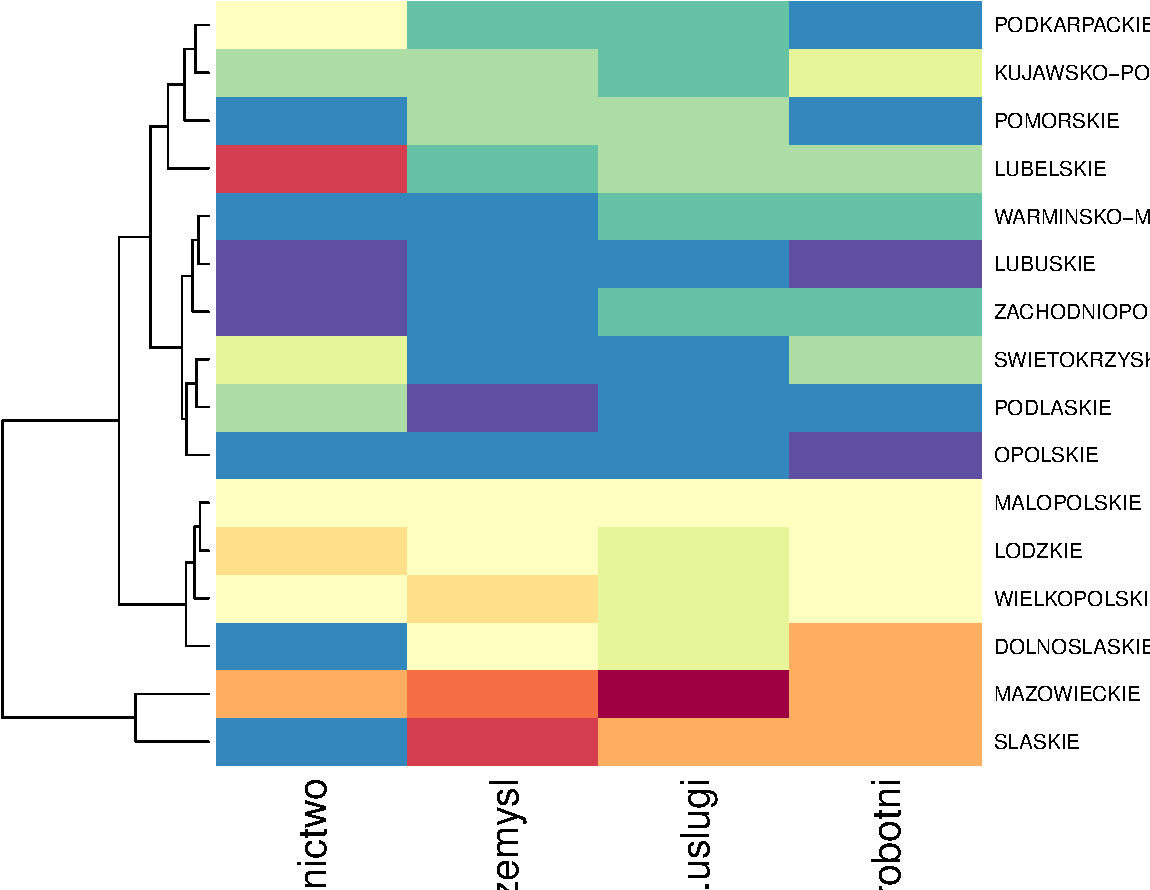
\includegraphics[width=0.7\linewidth]{NaPrzelajR_files/figure-latex/wy62A-1} 

}

\caption{Mapa ciepła dla danych oryginalnych (kolory normalizowane po kolumnach).}\label{fig:wy62A}
\end{figure}

\begin{Shaded}
\begin{Highlighting}[]
\CommentTok{# zobaczmy czy sa zaleznosci pomiedzy kolumnami i wierszami, wygląda na to że nie są to niezależne cechy}
\KeywordTok{chisq.test}\NormalTok{(dane)}
\end{Highlighting}
\end{Shaded}

\begin{verbatim}
## 
##  Pearson's Chi-squared test
## 
## data:  dane
## X-squared = 1031.9, df = 45, p-value < 2.2e-16
\end{verbatim}

Wykonaliśmy test \(\chi^2\) i otrzymaliśmy bardzo małą p-wartość, która upewniła nas w przekonaniu, że województwa mają inną strukturę zatrudnienia.

\begin{Shaded}
\begin{Highlighting}[]
\CommentTok{# zobaczmy które kombinacje występują częściej niż w przypadku niezależności}
\CommentTok{# policzymy residua Pearsonowskie}
\NormalTok{P =}\StringTok{ }\NormalTok{dane}\OperatorTok{/}\KeywordTok{sum}\NormalTok{(dane)}
\CommentTok{# macierz czestosci oczekiwanych}
\NormalTok{PP =}\StringTok{ }\KeywordTok{outer}\NormalTok{(}\KeywordTok{rowSums}\NormalTok{(P),}\KeywordTok{colSums}\NormalTok{(P))}
\CommentTok{# macierz residuow Pearsonowskich}
\NormalTok{E =}\StringTok{ }\NormalTok{(P}\OperatorTok{-}\NormalTok{PP)}\OperatorTok{/}\KeywordTok{sqrt}\NormalTok{(PP)}
\KeywordTok{head}\NormalTok{(E)}
\end{Highlighting}
\end{Shaded}

\begin{verbatim}
##                    pracujacy.rolnictwo pracujacy.przemysl pracujacy.uslugi
## DOLNOSLASKIE              -0.058854443        0.024423457      0.005571820
## KUJAWSKO-POMORSKIE         0.012508000        0.006942431     -0.016485942
## LODZKIE                    0.021307056        0.000860813     -0.012756112
## LUBELSKIE                  0.122091621       -0.046327197     -0.028293827
## LUBUSKIE                  -0.020324264        0.013026864      0.004913504
## MALOPOLSKIE                0.009798815       -0.004097028     -0.001688693
##                      bezrobotni
## DOLNOSLASKIE        0.022465943
## KUJAWSKO-POMORSKIE  0.015945574
## LODZKIE             0.003427270
## LUBELSKIE          -0.001528783
## LUBUSKIE           -0.013765063
## MALOPOLSKIE        -0.001118379
\end{verbatim}

\begin{Shaded}
\begin{Highlighting}[]
\CommentTok{# tę macierz również można przedstawić za pomocą mapy ciepła}
\KeywordTok{heatmap}\NormalTok{(E,}\DataTypeTok{scale=}\StringTok{"none"}\NormalTok{,}\DataTypeTok{Colv=}\OtherTok{NA}\NormalTok{,}\DataTypeTok{col=}\NormalTok{ kolory)}
\end{Highlighting}
\end{Shaded}

\begin{figure}[h]

{\centering 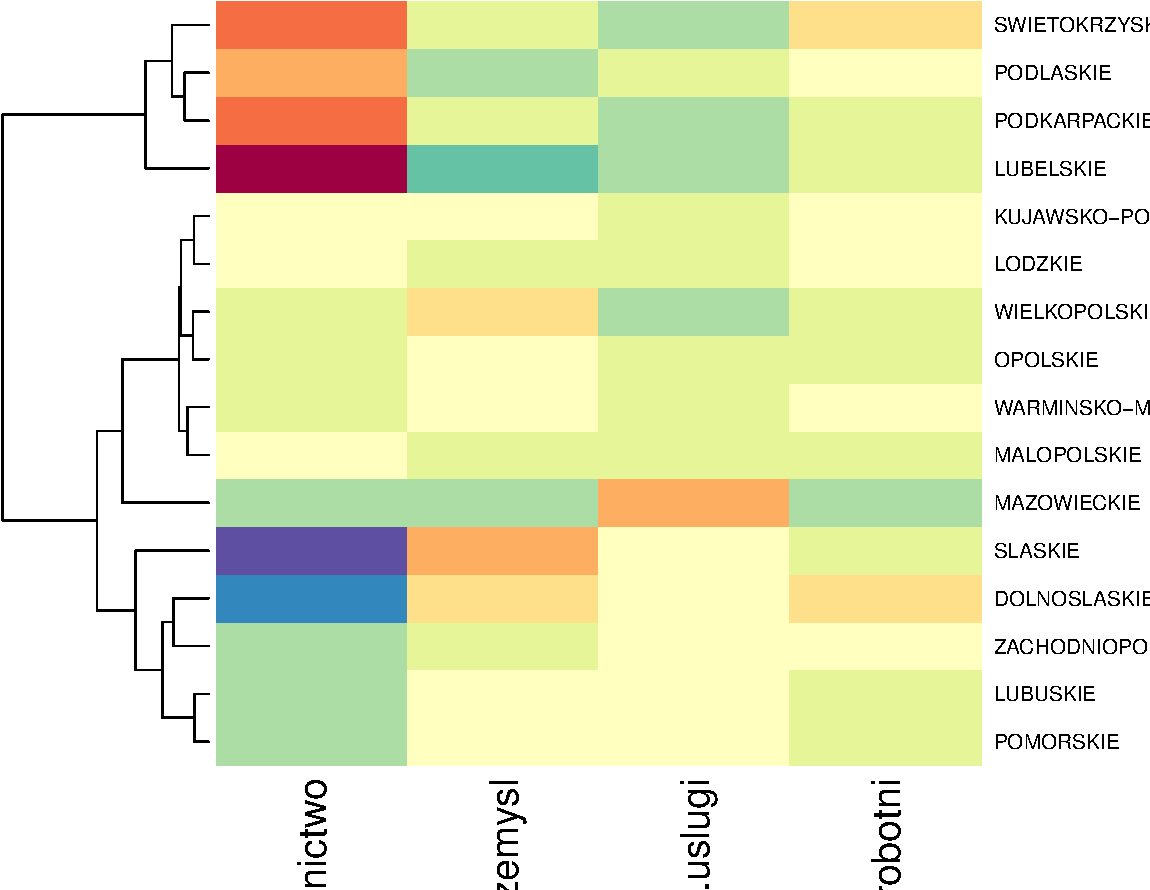
\includegraphics[width=0.7\linewidth]{NaPrzelajR_files/figure-latex/wy63A-1} 

}

\caption{Mapa ciepła dla reszt Pearsonowskich.}\label{fig:wy63A}
\end{figure}

Wyznaczyliśmy macierz reszt Pearsonowskich \(E\) (którą też przedstawiliśmy graficznie z użyciem mapy ciepła) i z tej macierzy możemy już odczytać w których
województwach poszczególne sektory są popularniejsze. Największe reszty obserwujemy dla sektora rolnictwa, zarówno duże dodatnie wartości (w województwie lubelskim, podlaskim, podkarpackim i świętokrzyskim) jak i duże (co do modułu) ujemne wartości (w województwie śląskim i dolnośląskim).
Możemy teraz przedstawić graficznie macierz \(E\) z użyciem biplotu (z wykorzystaniem dekompozycji SVD).

\begin{Shaded}
\begin{Highlighting}[]
\CommentTok{# wykonujemy dekompozycje na wartosci osobliwe (singularne/szczegolne)}
\NormalTok{A =}\StringTok{ }\KeywordTok{svd}\NormalTok{(E)}
\NormalTok{X =}\StringTok{ }\KeywordTok{t}\NormalTok{(}\KeywordTok{apply}\NormalTok{(A}\OperatorTok{$}\NormalTok{u, }\DecValTok{1}\NormalTok{, }\StringTok{"*"}\NormalTok{, }\KeywordTok{sqrt}\NormalTok{(A}\OperatorTok{$}\NormalTok{d)))}
\NormalTok{Y =}\StringTok{ }\KeywordTok{t}\NormalTok{(}\KeywordTok{apply}\NormalTok{(A}\OperatorTok{$}\NormalTok{v, }\DecValTok{1}\NormalTok{, }\StringTok{"*"}\NormalTok{, }\KeywordTok{sqrt}\NormalTok{(A}\OperatorTok{$}\NormalTok{d)))}
\CommentTok{# zwykle współrzędne liczone są ze wzorow, w ktorych A jest dekompozycja innej macierzy}
\CommentTok{# [}\AlertTok{TODO}\CommentTok{: uzupełnić albo pominąć]}
\CommentTok{# A = Dr^(-1/2) A$u A$d}
\CommentTok{# B = Dc^(-1/2) A$v a$d}
\end{Highlighting}
\end{Shaded}

\begin{Shaded}
\begin{Highlighting}[]
\KeywordTok{plot}\NormalTok{(}\KeywordTok{rbind}\NormalTok{(X[,}\DecValTok{1}\OperatorTok{:}\DecValTok{2}\NormalTok{], Y[,}\DecValTok{1}\OperatorTok{:}\DecValTok{2}\NormalTok{]), }\DataTypeTok{xlab=}\StringTok{""}\NormalTok{, }\DataTypeTok{ylab=}\StringTok{""}\NormalTok{, }\DataTypeTok{main=}\StringTok{"Bramka nr. 1"}\NormalTok{, lwd}
\NormalTok{=}\DecValTok{3}\NormalTok{)}
\end{Highlighting}
\end{Shaded}

\begin{figure}[h]

{\centering 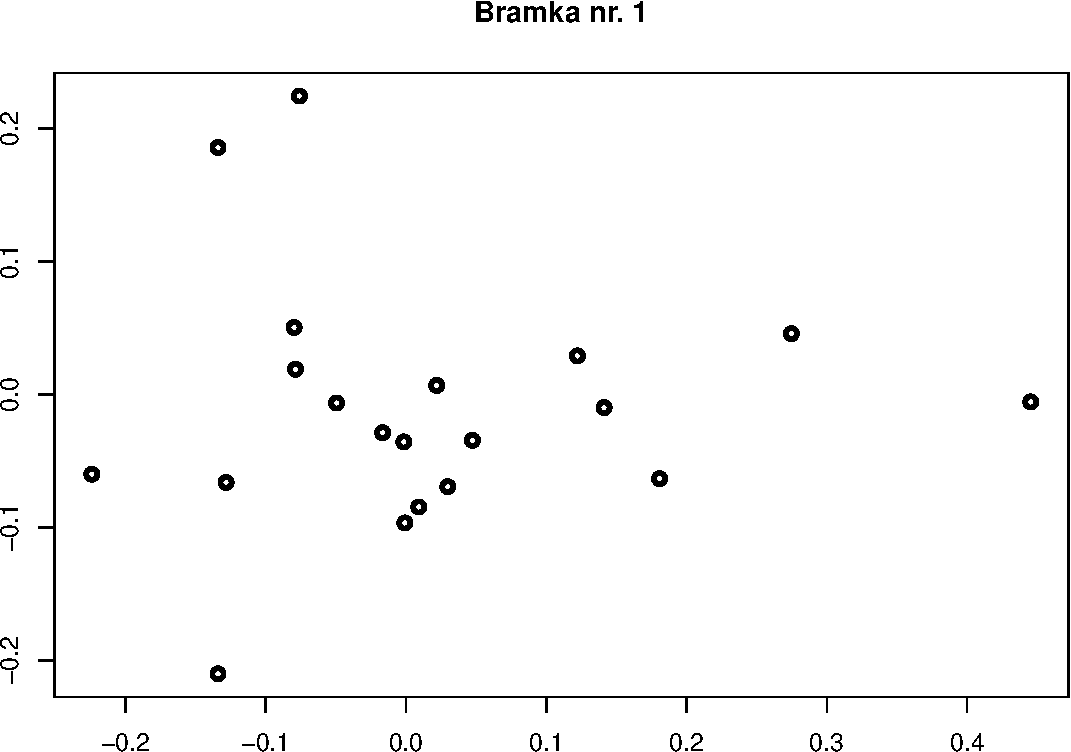
\includegraphics[width=0.7\linewidth]{NaPrzelajR_files/figure-latex/wy64A-1} 

}

\caption{?}\label{fig:wy64A}
\end{figure}

\begin{Shaded}
\begin{Highlighting}[]
\CommentTok{# analiza korespondencji z użyciem pakietu MASS}
\KeywordTok{biplot}\NormalTok{(MASS}\OperatorTok{::}\KeywordTok{corresp}\NormalTok{(dane, }\DataTypeTok{nf =} \DecValTok{2}\NormalTok{))}
\end{Highlighting}
\end{Shaded}

\begin{figure}[h]

{\centering 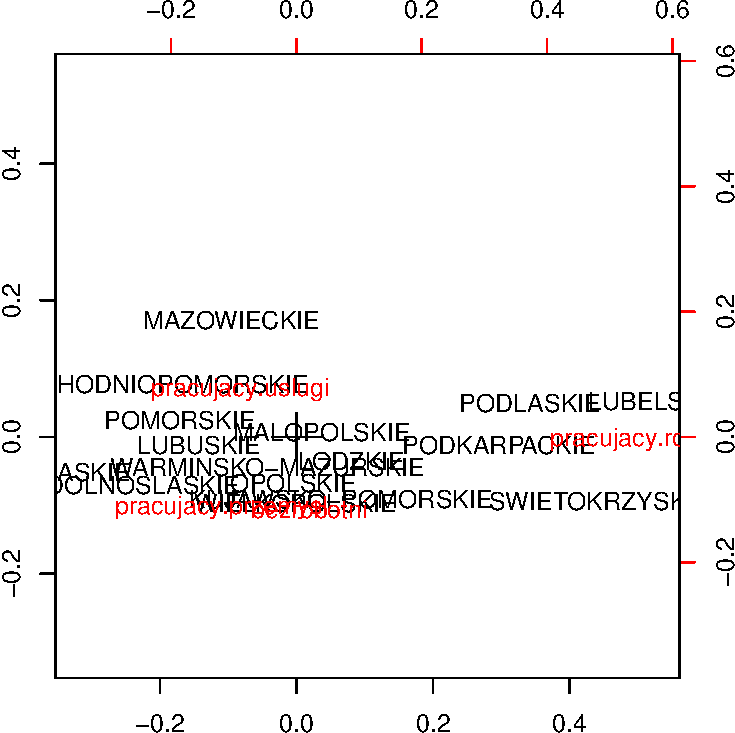
\includegraphics[width=0.7\linewidth]{NaPrzelajR_files/figure-latex/wy65A-1} 

}

\caption{?}\label{fig:wy65A}
\end{figure}

\begin{Shaded}
\begin{Highlighting}[]
\CommentTok{# analiza korespondencji z użyciem pakietu ca}
\CommentTok{# argument mass powoduje że liczebności komórek odpowiadają wielkościom punktów na wykresie}
\KeywordTok{plot}\NormalTok{(ca}\OperatorTok{::}\KeywordTok{ca}\NormalTok{(dane), }\DataTypeTok{mass=}\KeywordTok{c}\NormalTok{(T,T))}
\end{Highlighting}
\end{Shaded}

\begin{figure}[h]

{\centering 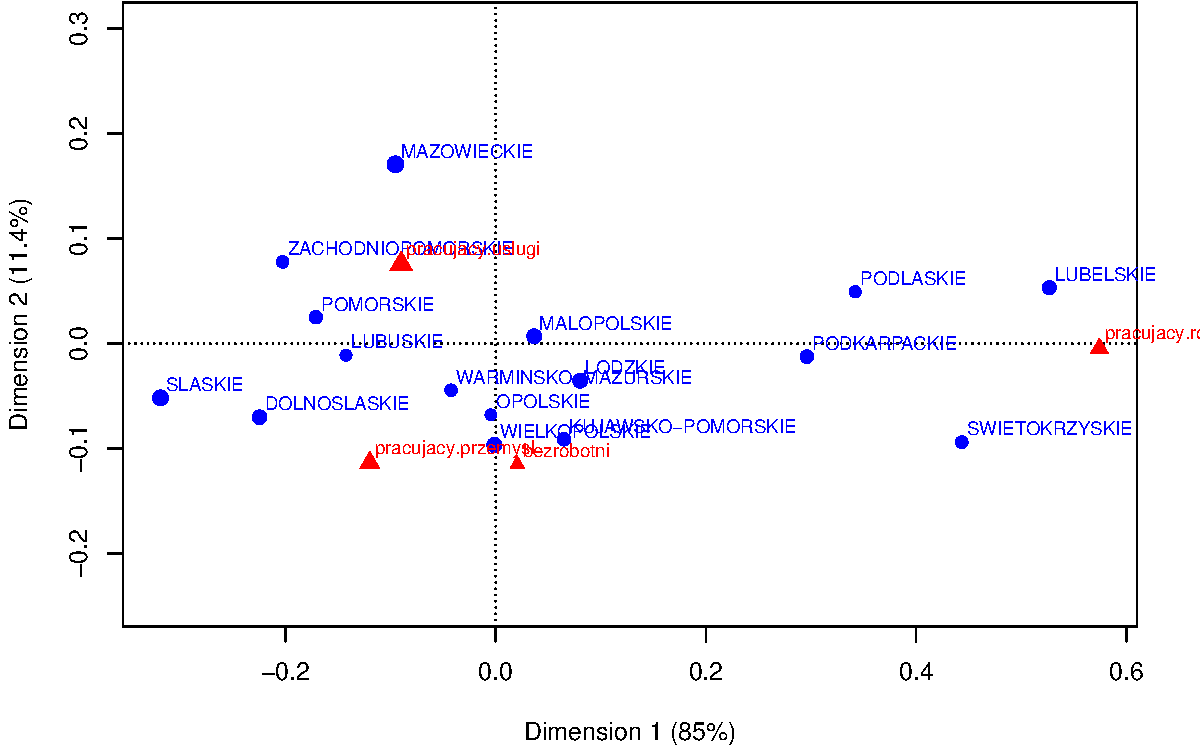
\includegraphics[width=0.7\linewidth]{NaPrzelajR_files/figure-latex/wy66A-1} 

}

\caption{Przykład analizy korespondencji.}\label{fig:wy66A}
\end{figure}

\begin{Shaded}
\begin{Highlighting}[]
\KeywordTok{summary}\NormalTok{(ca}\OperatorTok{::}\KeywordTok{ca}\NormalTok{(dane))}
\end{Highlighting}
\end{Shaded}

\begin{verbatim}
## 
## Principal inertias (eigenvalues):
## 
##  dim    value      %   cum%   scree plot               
##  1      0.054859  85.0  85.0  *********************    
##  2      0.007352  11.4  96.3  ***                      
##  3      0.002360   3.7 100.0  *                        
##         -------- -----                                 
##  Total: 0.064571 100.0                                 
## 
## 
## Rows:
##      name   mass  qlt  inr    k=1 cor ctr    k=2 cor ctr  
## 1  | DOLN |   76  918   71 | -225 837  70 |  -70  81  51 |
## 2  | KUJA |   49  848   11 |   65 286   4 |  -91 563  56 |
## 3  | LODZ |   82 1000   10 |   80 838  10 |  -35 162  14 |
## 4  | LUBE |   64 1000  277 |  527 990 322 |   53  10  24 |
## 5  | LUBU |   28  723   12 | -142 719  10 |  -11   4   0 |
## 6  | MALO |   84  995    2 |   37 960   2 |    7  34   1 |
## 7  | MAZO |  148 1000   88 |  -95 238  25 |  171 762 587 |
## 8  | OPOL |   24  496    3 |   -5   2   0 |  -68 494  15 |
## 9  | PODK |   53  926   78 |  296 925  85 |  -12   2   1 |
## 10 | PODL |   30  994   56 |  342 974  64 |   49  20  10 |
## 11 | POMO |   50  939   24 | -171 919  26 |   25  20   4 |
## 12 | SLAS |  115  995  187 | -319 970 214 |  -52  25  42 |
## 13 | SWIE |   39  968  128 |  443 926 139 |  -94  41  47 |
## 14 | WARM |   36  515    4 |  -42 246   1 |  -44 269  10 |
## 15 | WIEL |   86  808   15 |   -1   0   0 |  -97 808 109 |
## 16 | ZACH |   36  806   33 | -203 702  27 |   78 103  30 |
## 
## Columns:
##        name   mass  qlt  inr    k=1 cor ctr    k=2 cor ctr  
## 1 | prcjcyr |  141  999  720 |  574 999 847 |   -4   0   0 |
## 2 | prcjcyp |  293  967  128 | -120 509  77 | -114 458 514 |
## 3 | prcjcys |  520 1000  111 |  -90 587  77 |   75 413 402 |
## 4 |    bzrb |   46  236   42 |   21   7   0 | -115 228  83 |
\end{verbatim}

Przy opisie analizy korespondencji często wymienianym czynnikiem jest inercja, nazywana czasem bezwładnością (przez podobieństwo do inercji w fizyce). Aby
opisać formalnie czym jest ta miara musimy zacząć od kilku innych pojęć.

Niech masa wiersza i masa kolumny będzie określona jako brzegowe częstości
macierzy kontyngencji.

\begin{Shaded}
\begin{Highlighting}[]
\NormalTok{(}\DataTypeTok{masa.kolumny =} \KeywordTok{colSums}\NormalTok{(}\KeywordTok{prop.table}\NormalTok{(dane)))}
\end{Highlighting}
\end{Shaded}

\begin{verbatim}
## pracujacy.rolnictwo  pracujacy.przemysl    pracujacy.uslugi 
##          0.14072962          0.29284776          0.51992992 
##          bezrobotni 
##          0.04649271
\end{verbatim}

\begin{Shaded}
\begin{Highlighting}[]
\NormalTok{(}\DataTypeTok{masa.wiersza =} \KeywordTok{rowSums}\NormalTok{(}\KeywordTok{prop.table}\NormalTok{(dane)))}
\end{Highlighting}
\end{Shaded}

\begin{verbatim}
##        DOLNOSLASKIE  KUJAWSKO-POMORSKIE             LODZKIE 
##          0.07621551          0.04949628          0.08159690 
##           LUBELSKIE            LUBUSKIE         MALOPOLSKIE 
##          0.06370064          0.02822101          0.08359927 
##         MAZOWIECKIE            OPOLSKIE        PODKARPACKIE 
##          0.14848883          0.02371566          0.05331331 
##           PODLASKIE           POMORSKIE             SLASKIE 
##          0.02991052          0.04955885          0.11544960 
##      SWIETOKRZYSKIE WARMINSKO-MAZURSKIE       WIELKOPOLSKIE 
##          0.03892122          0.03585508          0.08578937 
##  ZACHODNIOPOMORSKIE 
##          0.03616795
\end{verbatim}

Profilem wiersza (kolumny) będą wartości w wierszu (kolumnie) unormowane
przez masę kolumny (wiersza).

\begin{Shaded}
\begin{Highlighting}[]
\KeywordTok{head}\NormalTok{(profil.kolumny <-}\StringTok{ }\NormalTok{dane}\OperatorTok{/}\KeywordTok{rowSums}\NormalTok{(dane))}
\end{Highlighting}
\end{Shaded}

\begin{verbatim}
##                    pracujacy.rolnictwo pracujacy.przemysl pracujacy.uslugi
## DOLNOSLASKIE                0.06075534          0.3407225        0.5344828
## KUJAWSKO-POMORSKIE          0.16182048          0.3097345        0.4664981
## LODZKIE                     0.16871166          0.2944785        0.4877301
## LUBELSKIE                   0.32220039          0.1935167        0.4390963
## LUBUSKIE                    0.09534368          0.3348115        0.5410200
## MALOPOLSKIE                 0.15344311          0.2851796        0.5157186
##                    bezrobotni
## DOLNOSLASKIE       0.06403941
## KUJAWSKO-POMORSKIE 0.06194690
## LODZKIE            0.04907975
## LUBELSKIE          0.04518664
## LUBUSKIE           0.02882483
## MALOPOLSKIE        0.04565868
\end{verbatim}

Tak unormowane profile wierszy i kolumn mogą być ze sobą porównywane. Im
większa odległość pomiędzy profilami kolumn tym mniejsza zależność pomiędzy
czynnikami opisanymi w tych kolumnach (oczywiście dla wierszy jest tak samo).
Średni profil kolumnowy to masa wiersza a średni profil wierszowy to masa kolumn.

Inercja to odległość (w mierze \(\chi^2\) ) pomiędzy daną kolumną (wierszem, punktem)
a średnią wartością dla kolumn (wierszy). Całkowita inercja to suma odległości dla
wszystkich kolumn (wierszy). \textbf{Im większa inercja tym punkty są oddalone
dalej od średniego profilu wiersza/kolumny}.

{[}TODO: uzupełnić. nawiązać do wyników funkcji summary.ca(){]}

Wyniki powyższych instrukcji oglądać można na wykresie \ref{fig:wy62A} i kolejnych.

Analizując ten wykres można zauważyć ciekawe zróżnicowanie województw. Na
osi X największą współrzędną ma zmienna \texttt{pr.rolnictwo}, a więc to ta zmienna odpowiada największemu zróżnicowaniu województw. Wysoki wartości na tej osi osiągają województwa gdzie zatrudnienie w rolnictwie było wyższe niż średnie. Druga
oś rozróżnia województwa w których dominuje zatrudnienie w sektorze usług (dodatnie wartości) versus zatrudnieniu w przemyśle lub braku zatrudnienia (niestety
profil zatrudnienia w przemyśle i braku zatrudnienia jest podobny).

Osoby w województwach Mazowieckim i Zachodniopomorskim częściej pracują
w sektorze usług, w województwach Lubelskim, Podlaskim, Świętokrzyskim i Podkarpackim dominuje zatrudnienie w sektorze rolniczym, w województwach Śląskim i
Dolnośląskim dominuje zatrudnienie w przemyśle te województwa mają też większe
problemy z bezrobociem.

{[}TODO: opisać podobieństwa i różnice do PCA{]}

\hypertarget{part_7}{%
\chapter{Przykład analizy szeregów czasowych}\label{part_7}}

\begin{center}\rule{0.5\linewidth}{\linethickness}\end{center}

\hypertarget{part_71}{%
\section{Wprowadzenie}\label{part_71}}

W skład szeregu czasowego mogą wchodzić następujące elementy:

\begin{itemize}
\item
  trend

  \begin{itemize}
  \item
    deterministyczny
  \item
    stochastyczny
  \end{itemize}
\item
  wahania sezonowe

  \begin{itemize}
  \item
    addytywne
  \item
    multiplikatywne
  \end{itemize}
\end{itemize}

\begin{Shaded}
\begin{Highlighting}[]
\KeywordTok{par}\NormalTok{(}\DataTypeTok{mfcol=}\KeywordTok{c}\NormalTok{(}\DecValTok{1}\NormalTok{,}\DecValTok{2}\NormalTok{),}\DataTypeTok{mar=}\KeywordTok{c}\NormalTok{(}\DecValTok{4}\NormalTok{,}\DecValTok{4}\NormalTok{,}\DecValTok{1}\NormalTok{,}\DecValTok{1}\NormalTok{)}\OperatorTok{+}\FloatTok{0.1}\NormalTok{, }\DataTypeTok{mgp=}\KeywordTok{c}\NormalTok{(}\DecValTok{3}\NormalTok{,}\FloatTok{0.6}\NormalTok{,}\DecValTok{0}\NormalTok{),}\DataTypeTok{las=}\DecValTok{1}\NormalTok{)}
\KeywordTok{plot}\NormalTok{(}\KeywordTok{log}\NormalTok{(AirPassengers),}\DataTypeTok{col=}\StringTok{"SteelBlue"}\NormalTok{); }\KeywordTok{title}\NormalTok{(}\StringTok{"addytywny"}\NormalTok{)}
\KeywordTok{plot}\NormalTok{(AirPassengers,}\DataTypeTok{col=}\StringTok{"SteelBlue"}\NormalTok{); }\KeywordTok{title}\NormalTok{(}\StringTok{"multiplikatywwny"}\NormalTok{)}
\end{Highlighting}
\end{Shaded}

\begin{figure}[h]

{\centering 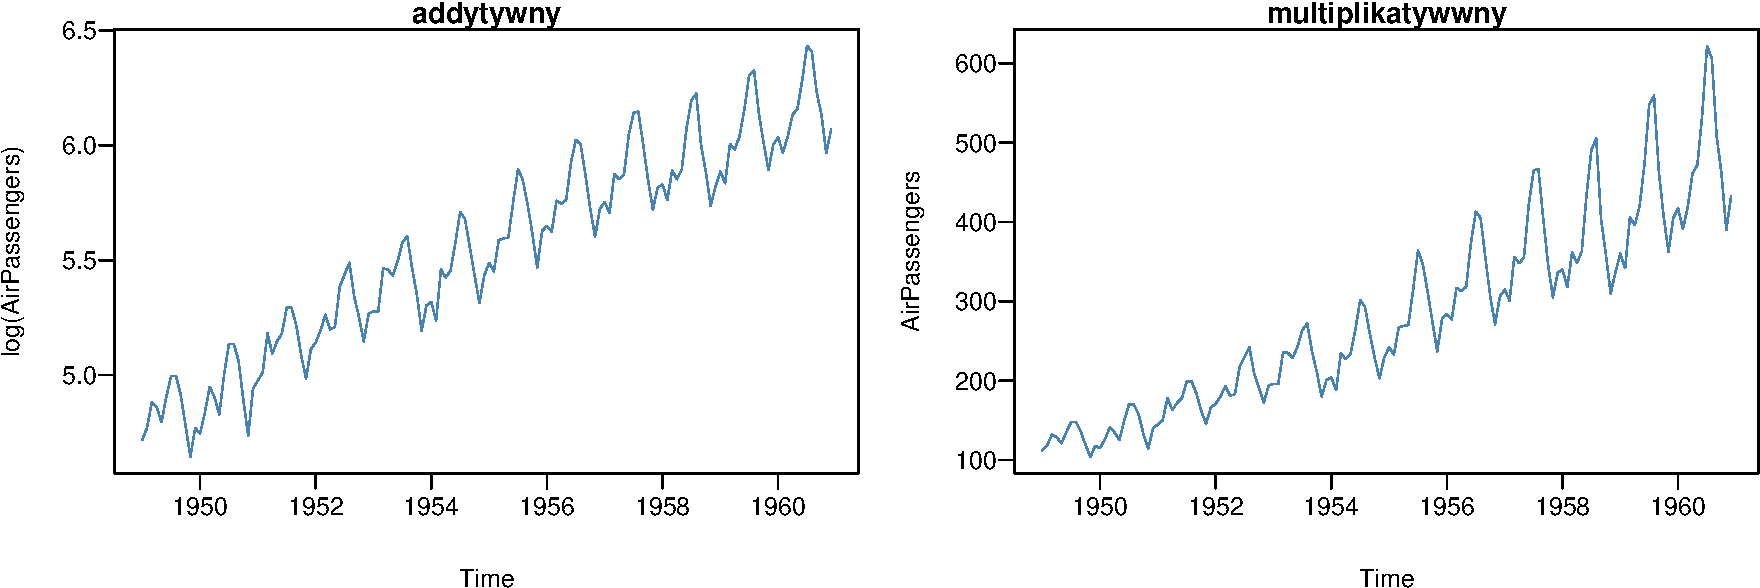
\includegraphics[width=1\linewidth]{NaPrzelajR_files/figure-latex/wy71-1} 

}

\caption{Przykłady szeregów czasowych.}\label{fig:wy71}
\end{figure}

Wśród szeregów czasowych rozróżniamy dwa rodzaje procesów stochastycznych:
stacjonarne (w których nie występuje trend) oraz niestacjonarne (w których występuje trend). Aby wyeliminować tendencję rozwojową z danego procesu można
wykorzystać do tego celu różnicowanie:

\begin{itemize}
\tightlist
\item
  jednokrotne różnicowanie:
\end{itemize}

\begin{equation}
\Delta y_t=y_t-y_{t-1}
\label{eq:wz01}
\end{equation}

\begin{Shaded}
\begin{Highlighting}[]
\NormalTok{dy <-}\StringTok{ }\KeywordTok{diff}\NormalTok{(AirPassengers)}
\end{Highlighting}
\end{Shaded}

\begin{itemize}
\tightlist
\item
  dwukrotne różnicowanie:
\end{itemize}

\begin{equation}
\Delta\Delta y_t=y_t-y_{t-1}
\label{eq:wz02}
\end{equation}

\begin{Shaded}
\begin{Highlighting}[]
\NormalTok{ddy <-}\StringTok{ }\KeywordTok{diff}\NormalTok{(AirPassengers, }\DataTypeTok{lag=} \DecValTok{1}\NormalTok{, }\DataTypeTok{differences=} \DecValTok{2}\NormalTok{)}
\end{Highlighting}
\end{Shaded}

\begin{Shaded}
\begin{Highlighting}[]
\KeywordTok{par}\NormalTok{(}\DataTypeTok{mfcol=}\KeywordTok{c}\NormalTok{(}\DecValTok{1}\NormalTok{,}\DecValTok{2}\NormalTok{),}\DataTypeTok{mar=}\KeywordTok{c}\NormalTok{(}\DecValTok{4}\NormalTok{,}\DecValTok{4}\NormalTok{,}\DecValTok{1}\NormalTok{,}\DecValTok{1}\NormalTok{)}\OperatorTok{+}\FloatTok{0.1}\NormalTok{, }\DataTypeTok{mgp=}\KeywordTok{c}\NormalTok{(}\DecValTok{3}\NormalTok{,}\FloatTok{0.6}\NormalTok{,}\DecValTok{0}\NormalTok{),}\DataTypeTok{las=}\DecValTok{1}\NormalTok{)}
\KeywordTok{plot}\NormalTok{(}\KeywordTok{diff}\NormalTok{(}\KeywordTok{log}\NormalTok{(AirPassengers)),}\DataTypeTok{col=}\StringTok{"SteelBlue"}\NormalTok{); }\KeywordTok{title}\NormalTok{(}\StringTok{"addytywny"}\NormalTok{)}
\KeywordTok{plot}\NormalTok{(}\KeywordTok{diff}\NormalTok{(AirPassengers),}\DataTypeTok{col=}\StringTok{"SteelBlue"}\NormalTok{); }\KeywordTok{title}\NormalTok{(}\StringTok{"multiplikatywwny"}\NormalTok{)}
\end{Highlighting}
\end{Shaded}

\begin{figure}[h]

{\centering 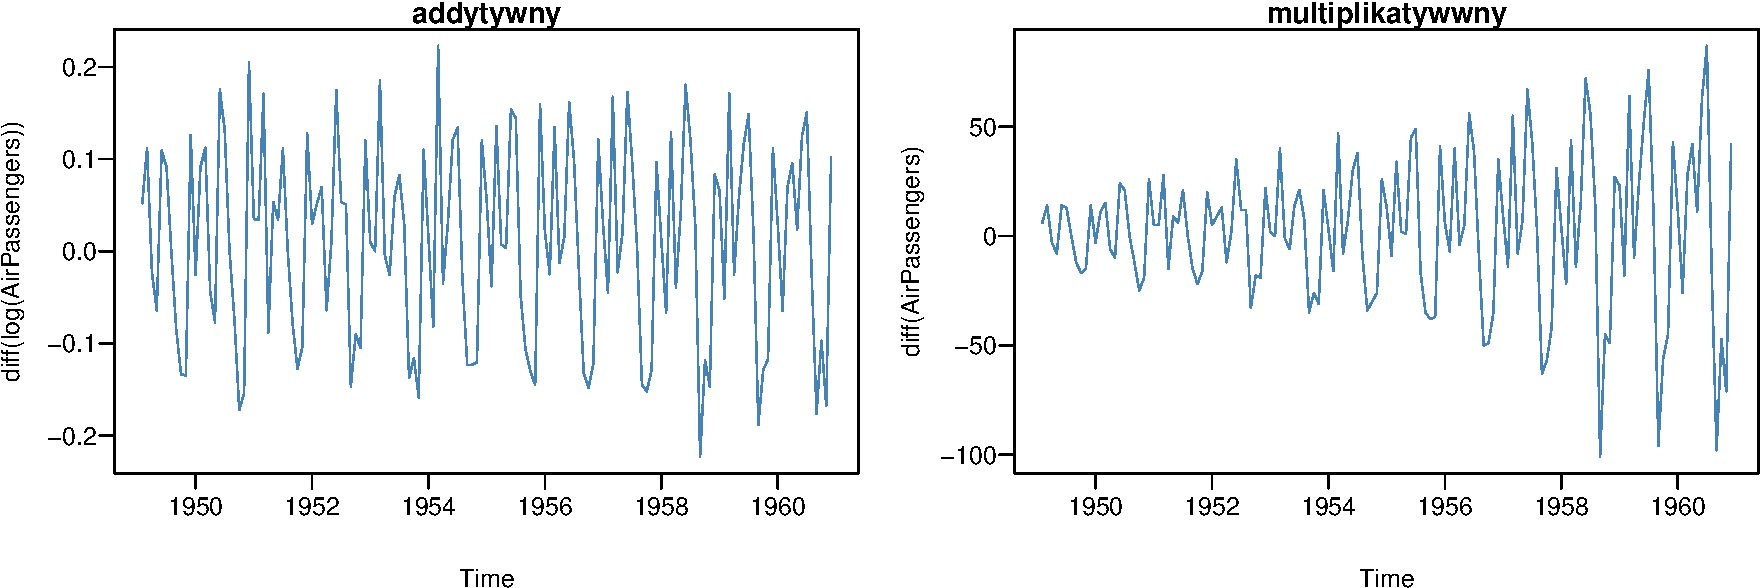
\includegraphics[width=1\linewidth]{NaPrzelajR_files/figure-latex/wy72-1} 

}

\caption{Przykłady jednokrotnego różnicowania szeregów czasowych.}\label{fig:wy72}
\end{figure}

W środowisku R dostępne są także funkcje dotyczące filtrowania szeregów czasowych. Jest to takie przekształcenie danych które doprowadza do oczyszczenia szeregu
czasowego z wahań periodycznych. W środowisku R dostępnych jest kilka takich
filtrów. Jeden z bardzie popularnych to filtr Hodrick-Prescotta zaimplementowany w pakiecie \href{https://rdrr.io/cran/FRAPO/man/trdhp.html}{FRAPO::trdhp}. Stosując filtr HP należy pamiętać o odpowiednim doborze parametru \(\lambda\). Hodrick oraz Prescott zalecają, aby wartość współczynnika \(\lambda\) była równa 400, 1600 i 14400
odpowiednio dla danych rocznych, kwartalnych i miesięcznych.

\begin{Shaded}
\begin{Highlighting}[]
\NormalTok{f <-}\StringTok{ }\NormalTok{FRAPO}\OperatorTok{::}\KeywordTok{trdhp}\NormalTok{(AirPassengers, }\DataTypeTok{lambda=}\DecValTok{14400}\NormalTok{)}

\KeywordTok{par}\NormalTok{(}\DataTypeTok{mfcol=}\KeywordTok{c}\NormalTok{(}\DecValTok{2}\NormalTok{,}\DecValTok{1}\NormalTok{),}\DataTypeTok{mar=}\KeywordTok{c}\NormalTok{(}\DecValTok{4}\NormalTok{,}\DecValTok{4}\NormalTok{,}\DecValTok{1}\NormalTok{,}\DecValTok{1}\NormalTok{)}\OperatorTok{+}\FloatTok{0.1}\NormalTok{, }\DataTypeTok{mgp=}\KeywordTok{c}\NormalTok{(}\DecValTok{3}\NormalTok{,}\FloatTok{0.6}\NormalTok{,}\DecValTok{0}\NormalTok{),}\DataTypeTok{las=}\DecValTok{1}\NormalTok{)}
\KeywordTok{plot}\NormalTok{(AirPassengers,}\DataTypeTok{col=}\StringTok{"SteelBlue"}\NormalTok{,}
     \DataTypeTok{main=}\StringTok{"Hodrick-Prescott filter"}\NormalTok{)}
\KeywordTok{lines}\NormalTok{(f,}\DataTypeTok{col=}\StringTok{"YellowGreen"}\NormalTok{)}
\KeywordTok{plot}\NormalTok{(AirPassengers}\OperatorTok{-}\NormalTok{f,}\DataTypeTok{col=}\StringTok{"SteelBlue"}\NormalTok{,}
     \DataTypeTok{main=}\StringTok{"Cyclical component (deviations from trend)"}\NormalTok{)}
\end{Highlighting}
\end{Shaded}

\begin{figure}[h]

{\centering 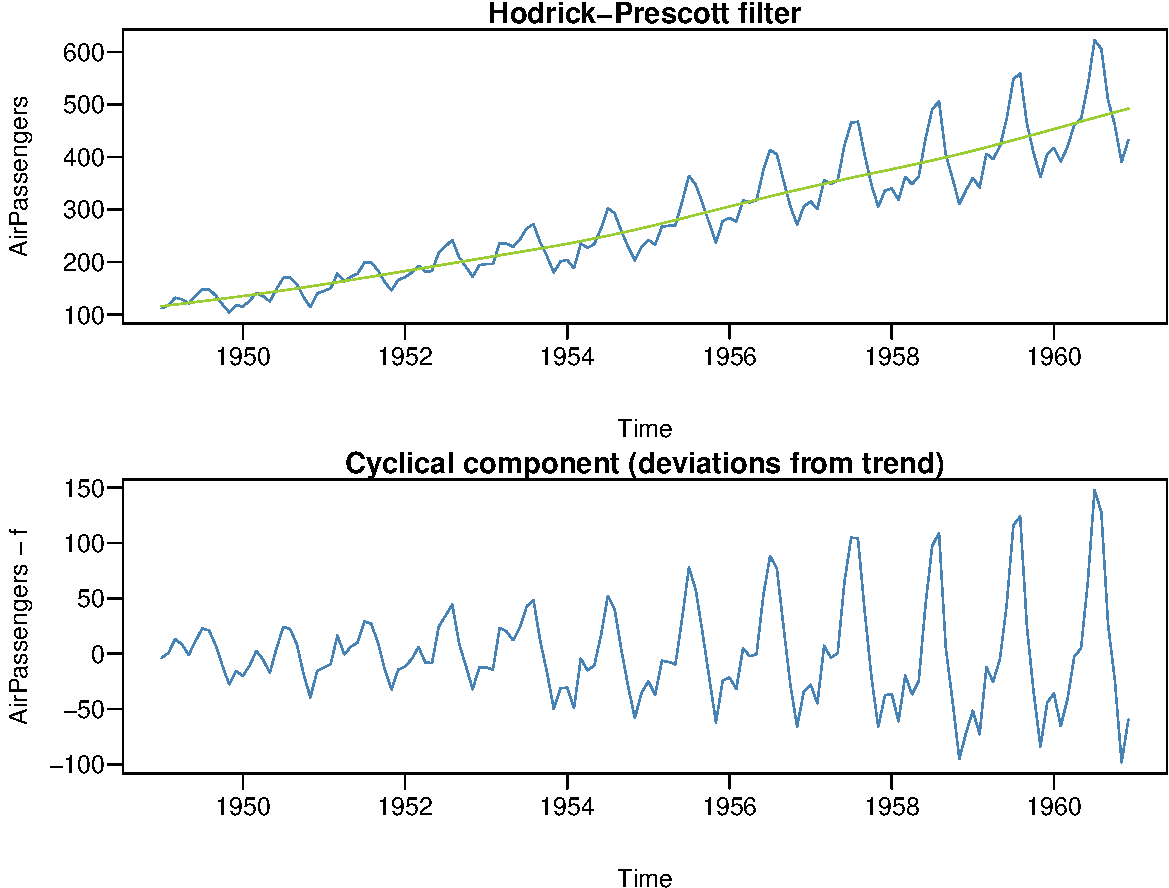
\includegraphics[width=0.7\linewidth]{NaPrzelajR_files/figure-latex/wy73-1} 

}

\caption{Filtr Hodrick-Prescott.}\label{fig:wy73}
\end{figure}

Dodajmy, że lepszą alternatywę dla procedury Hodricka-Prescotta zaproponował James D. Hamilton. Ten filtr został zaimplementowany do funkcji \href{https://rdrr.io/cran/neverhpfilter/man/yth_filter.html}{neverhpfilter::yth\_filter}.

\hypertarget{part_72}{%
\section{Identyfikacja trendu i sezonowości}\label{part_72}}

\hypertarget{part_721}{%
\subsection{Analiza wariancji - ANOVA}\label{part_721}}

Ocena występowania trendu oraz wahań periodycznych zostanie dokonana na przykładzie miesięcznej stopy bezrobocia w Polsce w okresie od 01-2004 do 10-2010 roku.

\begin{Shaded}
\begin{Highlighting}[]
\NormalTok{b <-}\StringTok{ }\KeywordTok{c}\NormalTok{(}\FloatTok{20.6}\NormalTok{, }\FloatTok{20.6}\NormalTok{, }\FloatTok{20.4}\NormalTok{, }\FloatTok{19.9}\NormalTok{, }\FloatTok{19.5}\NormalTok{, }\FloatTok{19.4}\NormalTok{, }\FloatTok{19.3}\NormalTok{, }\FloatTok{19.1}\NormalTok{, }\FloatTok{18.9}\NormalTok{, }\FloatTok{18.7}\NormalTok{, }\FloatTok{18.7}\NormalTok{, }\FloatTok{19.0}\NormalTok{, }\FloatTok{19.4}\NormalTok{, }\FloatTok{19.4}\NormalTok{, }
       \FloatTok{19.2}\NormalTok{, }\FloatTok{18.7}\NormalTok{, }\FloatTok{18.2}\NormalTok{, }\FloatTok{18.0}\NormalTok{, }\FloatTok{17.9}\NormalTok{, }\FloatTok{17.7}\NormalTok{, }\FloatTok{17.6}\NormalTok{, }\FloatTok{17.3}\NormalTok{, }\FloatTok{17.3}\NormalTok{, }\FloatTok{17.6}\NormalTok{, }\FloatTok{18.0}\NormalTok{, }\FloatTok{18.0}\NormalTok{, }\FloatTok{17.8}\NormalTok{, }\FloatTok{17.2}\NormalTok{,}
       \FloatTok{16.5}\NormalTok{, }\FloatTok{16.0}\NormalTok{, }\FloatTok{15.7}\NormalTok{, }\FloatTok{15.5}\NormalTok{, }\FloatTok{15.2}\NormalTok{, }\FloatTok{14.9}\NormalTok{, }\FloatTok{14.8}\NormalTok{, }\FloatTok{14.9}\NormalTok{, }\FloatTok{15.1}\NormalTok{, }\FloatTok{14.9}\NormalTok{, }\FloatTok{14.4}\NormalTok{, }\FloatTok{13.7}\NormalTok{, }\FloatTok{13.0}\NormalTok{, }\FloatTok{12.4}\NormalTok{,}
       \FloatTok{12.2}\NormalTok{, }\FloatTok{11.9}\NormalTok{, }\FloatTok{11.6}\NormalTok{, }\FloatTok{11.3}\NormalTok{, }\FloatTok{11.3}\NormalTok{, }\FloatTok{11.4}\NormalTok{, }\FloatTok{11.7}\NormalTok{, }\FloatTok{11.5}\NormalTok{, }\FloatTok{11.1}\NormalTok{, }\FloatTok{10.5}\NormalTok{, }\FloatTok{10.0}\NormalTok{, }\FloatTok{9.6}\NormalTok{,  }\FloatTok{9.40}\NormalTok{, }\FloatTok{9.10}\NormalTok{,}
       \FloatTok{8.90}\NormalTok{, }\FloatTok{8.80}\NormalTok{, }\FloatTok{9.10}\NormalTok{, }\FloatTok{9.50}\NormalTok{, }\FloatTok{10.5}\NormalTok{, }\FloatTok{10.9}\NormalTok{, }\FloatTok{11.2}\NormalTok{, }\FloatTok{11.0}\NormalTok{, }\FloatTok{10.8}\NormalTok{, }\FloatTok{10.7}\NormalTok{, }\FloatTok{10.8}\NormalTok{, }\FloatTok{10.8}\NormalTok{, }\FloatTok{10.9}\NormalTok{, }\FloatTok{11.1}\NormalTok{,}
       \FloatTok{11.4}\NormalTok{, }\FloatTok{11.9}\NormalTok{, }\FloatTok{12.7}\NormalTok{, }\FloatTok{13.0}\NormalTok{, }\FloatTok{12.9}\NormalTok{, }\FloatTok{12.3}\NormalTok{, }\FloatTok{11.9}\NormalTok{, }\FloatTok{10.6}\NormalTok{, }\FloatTok{10.7}\NormalTok{, }\FloatTok{11.4}\NormalTok{, }\FloatTok{11.5}\NormalTok{)}
\NormalTok{b <-}\StringTok{ }\KeywordTok{ts}\NormalTok{(b, }\DataTypeTok{frequency =} \DecValTok{12}\NormalTok{, }\DataTypeTok{start =} \KeywordTok{c}\NormalTok{(}\DecValTok{2004}\NormalTok{, }\DecValTok{1}\NormalTok{))}
\end{Highlighting}
\end{Shaded}

\begin{Shaded}
\begin{Highlighting}[]
\KeywordTok{par}\NormalTok{(}\DataTypeTok{mar=}\KeywordTok{c}\NormalTok{(}\DecValTok{4}\NormalTok{,}\DecValTok{4}\NormalTok{,}\DecValTok{1}\NormalTok{,}\DecValTok{1}\NormalTok{)}\OperatorTok{+}\FloatTok{0.1}\NormalTok{, }\DataTypeTok{mgp=}\KeywordTok{c}\NormalTok{(}\DecValTok{3}\NormalTok{,}\FloatTok{0.6}\NormalTok{,}\DecValTok{0}\NormalTok{),}\DataTypeTok{las=}\DecValTok{1}\NormalTok{)}
\KeywordTok{plot}\NormalTok{(b,}\DataTypeTok{type=}\StringTok{"l"}\NormalTok{,}\DataTypeTok{col=}\StringTok{"SteelBlue"}\NormalTok{)}
\end{Highlighting}
\end{Shaded}

\begin{figure}[h]

{\centering 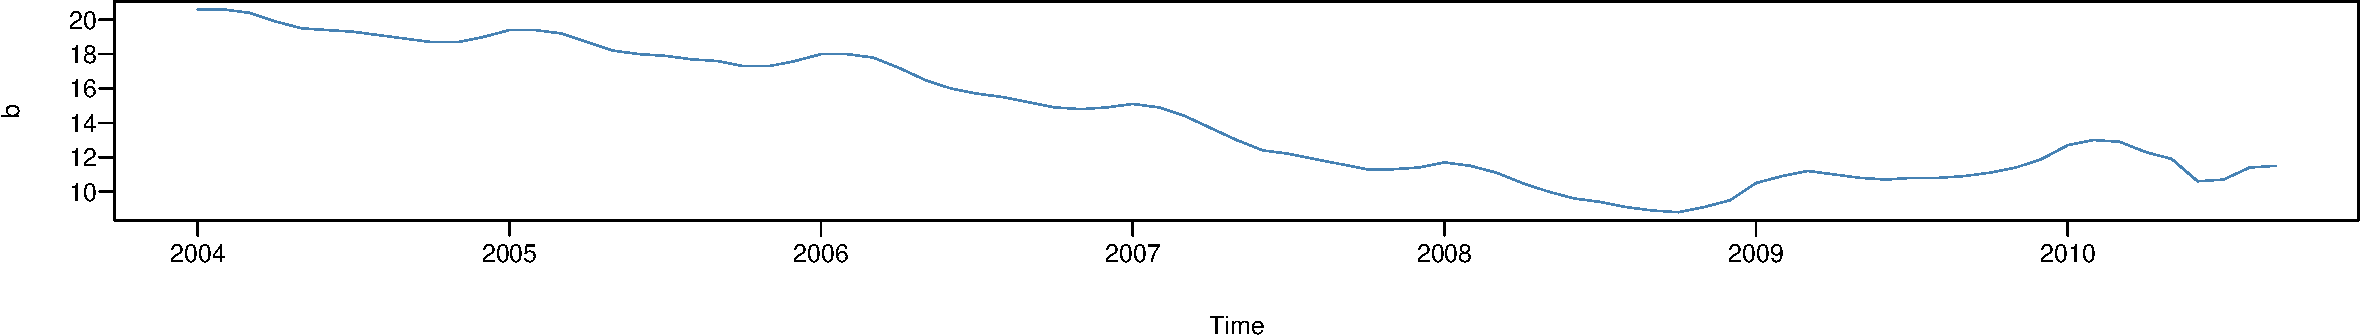
\includegraphics[width=0.7\linewidth]{NaPrzelajR_files/figure-latex/wy74-1} 

}

\caption{Stopa bezrobocia w Polsce od 01-2004 do 10-2010 roku.}\label{fig:wy74}
\end{figure}

\begin{Shaded}
\begin{Highlighting}[]
\NormalTok{T <-}\StringTok{ }\KeywordTok{rep}\NormalTok{(}\KeywordTok{c}\NormalTok{(}\DecValTok{2004}\NormalTok{,}\DecValTok{2005}\NormalTok{,}\DecValTok{2006}\NormalTok{,}\DecValTok{2007}\NormalTok{,}\DecValTok{2008}\NormalTok{,}\DecValTok{2009}\NormalTok{,}\DecValTok{2010}\NormalTok{),}\KeywordTok{c}\NormalTok{(}\DecValTok{12}\NormalTok{,}\DecValTok{12}\NormalTok{,}\DecValTok{12}\NormalTok{,}\DecValTok{12}\NormalTok{,}\DecValTok{12}\NormalTok{,}\DecValTok{12}\NormalTok{,}\DecValTok{9}\NormalTok{))}
\NormalTok{T <-}\StringTok{ }\KeywordTok{factor}\NormalTok{(T)}
\NormalTok{S <-}\StringTok{ }\KeywordTok{rep}\NormalTok{(}\DecValTok{1}\OperatorTok{:}\DecValTok{12}\NormalTok{,}\DecValTok{7}\NormalTok{);S=S[}\OperatorTok{-}\KeywordTok{c}\NormalTok{(}\DecValTok{82}\OperatorTok{:}\DecValTok{84}\NormalTok{)]}
\NormalTok{S <-}\StringTok{ }\KeywordTok{factor}\NormalTok{(S)}
\end{Highlighting}
\end{Shaded}

Identyfikację szeregu czasowego można przeprowadzić na kilka sposobów. Jednym z
nich jest analiza wariancji ANOVA.

\begin{Shaded}
\begin{Highlighting}[]
\KeywordTok{anova}\NormalTok{(}\KeywordTok{lm}\NormalTok{(b}\OperatorTok{~}\NormalTok{T}\OperatorTok{+}\NormalTok{S))}
\end{Highlighting}
\end{Shaded}

\begin{verbatim}
## Analysis of Variance Table
## 
## Response: b
##           Df Sum Sq Mean Sq F value    Pr(>F)    
## T          6 990.99 165.165 523.410 < 2.2e-16 ***
## S         11  51.67   4.697  14.886  1.13e-13 ***
## Residuals 63  19.88   0.316                      
## ---
## Signif. codes:  0 '***' 0.001 '**' 0.01 '*' 0.05 '.' 0.1 ' ' 1
\end{verbatim}

Na podstawie przeprowadzonej analizie wariancji, należy stwierdzić, że w omawianym szeregu czasowym występuje trend (p-value = 2.2e-16). W celu dokonania
dalszej identyfikacji szeregu (oceny występowania sezonowości) należy wyeliminować
tendencję rozwojową (np. poprzez różnicowanie).

\begin{Shaded}
\begin{Highlighting}[]
\KeywordTok{anova}\NormalTok{(}\KeywordTok{lm}\NormalTok{(}\KeywordTok{diff}\NormalTok{(b)}\OperatorTok{~}\NormalTok{T[}\OperatorTok{-}\DecValTok{1}\NormalTok{]}\OperatorTok{+}\NormalTok{S[}\OperatorTok{-}\DecValTok{1}\NormalTok{]))}
\end{Highlighting}
\end{Shaded}

\begin{verbatim}
## Analysis of Variance Table
## 
## Response: diff(b)
##           Df Sum Sq Mean Sq F value    Pr(>F)    
## T[-1]      6 1.7879 0.29798  8.1625 1.617e-06 ***
## S[-1]     11 6.8836 0.62578 17.1420 6.600e-15 ***
## Residuals 62 2.2634 0.03651                      
## ---
## Signif. codes:  0 '***' 0.001 '**' 0.01 '*' 0.05 '.' 0.1 ' ' 1
\end{verbatim}

Jednokrotne różnicowanie szeregu nie przyniosło porządanego efektu (p-value =
1.617e-06). Zatem powinniśmy badany szereg poddać dwukrotnemu różnicowaniu. Należy tę procedurę powtarzać, aż do skutku czyli wyeliminowamia trendu.

\begin{Shaded}
\begin{Highlighting}[]
\KeywordTok{anova}\NormalTok{(}\KeywordTok{lm}\NormalTok{(}\KeywordTok{diff}\NormalTok{(b,}\DecValTok{1}\NormalTok{,}\DecValTok{2}\NormalTok{)}\OperatorTok{~}\NormalTok{T[}\OperatorTok{-}\KeywordTok{c}\NormalTok{(}\DecValTok{1}\NormalTok{,}\DecValTok{2}\NormalTok{)]}\OperatorTok{+}\NormalTok{S[}\OperatorTok{-}\KeywordTok{c}\NormalTok{(}\DecValTok{1}\NormalTok{,}\DecValTok{2}\NormalTok{)]))}
\end{Highlighting}
\end{Shaded}

\begin{verbatim}
## Analysis of Variance Table
## 
## Response: diff(b, 1, 2)
##             Df Sum Sq Mean Sq F value    Pr(>F)    
## T[-c(1, 2)]  6 0.0383 0.00639  0.1030    0.9958    
## S[-c(1, 2)] 11 4.3495 0.39541  6.3775 6.621e-07 ***
## Residuals   61 3.7820 0.06200                      
## ---
## Signif. codes:  0 '***' 0.001 '**' 0.01 '*' 0.05 '.' 0.1 ' ' 1
\end{verbatim}

Dopiero dwukrotne różnicowanie przyniosło porządany efekt (p-value = 0.9958). Tak
więc teraz możemy stwierdzić, że w badanym szeregu czasowym występuje sezonowość (p-value = 6.621e-07).

\begin{Shaded}
\begin{Highlighting}[]
\KeywordTok{summary}\NormalTok{(}\KeywordTok{lm}\NormalTok{(b}\OperatorTok{~}\NormalTok{T}\OperatorTok{+}\NormalTok{S))}
\end{Highlighting}
\end{Shaded}

\begin{verbatim}
## 
## Call:
## lm(formula = b ~ T + S)
## 
## Residuals:
##      Min       1Q   Median       3Q      Max 
## -1.75126 -0.20245  0.02639  0.19755  1.45139 
## 
## Coefficients:
##             Estimate Std. Error t value Pr(>|t|)    
## (Intercept) 20.75959    0.26044  79.710  < 2e-16 ***
## T2005       -1.31667    0.22933  -5.741 2.91e-07 ***
## T2006       -3.30000    0.22933 -14.390  < 2e-16 ***
## T2007       -6.74167    0.22933 -29.397  < 2e-16 ***
## T2008       -9.57500    0.22933 -41.752  < 2e-16 ***
## T2009       -8.50833    0.22933 -37.101  < 2e-16 ***
## T2010       -7.87546    0.25064 -31.422  < 2e-16 ***
## S2           0.04286    0.30026   0.143 0.886958    
## S3          -0.14286    0.30026  -0.476 0.635883    
## S4          -0.67143    0.30026  -2.236 0.028894 *  
## S5          -1.15714    0.30026  -3.854 0.000275 ***
## S6          -1.61429    0.30026  -5.376 1.18e-06 ***
## S7          -1.71429    0.30026  -5.709 3.29e-07 ***
## S8          -1.78571    0.30026  -5.947 1.31e-07 ***
## S9          -1.91429    0.30026  -6.375 2.42e-08 ***
## S10         -2.16931    0.31386  -6.912 2.85e-09 ***
## S11         -2.08598    0.31386  -6.646 8.23e-09 ***
## S12         -1.80265    0.31386  -5.744 2.88e-07 ***
## ---
## Signif. codes:  0 '***' 0.001 '**' 0.01 '*' 0.05 '.' 0.1 ' ' 1
## 
## Residual standard error: 0.5617 on 63 degrees of freedom
## Multiple R-squared:  0.9813, Adjusted R-squared:  0.9762 
## F-statistic: 194.4 on 17 and 63 DF,  p-value: < 2.2e-16
\end{verbatim}

Oszacowane współczynniki regresji liniowej wskazują jakie są różnice między średnimi stapami bezrobocia w poszczególnych latach oraz miesiącach. Punktem referencyjnym dla czynnika \texttt{T} jest 2004 rok, dla \texttt{S} styczeń. Aby zmienić punkt odniesienia np. na rok 2005 wystarczy wykonać komendę:

\begin{Shaded}
\begin{Highlighting}[]
\NormalTok{T =}\StringTok{ }\KeywordTok{relevel}\NormalTok{(T, }\DataTypeTok{ref=}\StringTok{"2005"}\NormalTok{)}
\end{Highlighting}
\end{Shaded}

a następnie przeprowadzić regresję. Jeśli chcemy wyznaczyć średnie stopy bezrobocia
w poszczególnych latach trzeba skorzystać z funkcji \href{https://rdrr.io/r/base/tapply.html}{tapply}:

\begin{Shaded}
\begin{Highlighting}[]
\KeywordTok{tapply}\NormalTok{(b,T,mean)}
\end{Highlighting}
\end{Shaded}

\begin{verbatim}
##      2005      2004      2006      2007      2008      2009      2010 
## 18.191667 19.508333 16.208333 12.766667  9.933333 11.000000 11.888889
\end{verbatim}

Prezentację graficzną kształtowania się średnich możemy wykonać w następujący
sposób:

\begin{Shaded}
\begin{Highlighting}[]
\KeywordTok{par}\NormalTok{(}\DataTypeTok{mfcol=}\KeywordTok{c}\NormalTok{(}\DecValTok{1}\NormalTok{,}\DecValTok{2}\NormalTok{),}\DataTypeTok{mar=}\KeywordTok{c}\NormalTok{(}\DecValTok{4}\NormalTok{,}\DecValTok{4}\NormalTok{,}\DecValTok{1}\NormalTok{,}\DecValTok{1}\NormalTok{)}\OperatorTok{+}\FloatTok{0.1}\NormalTok{, }\DataTypeTok{mgp=}\KeywordTok{c}\NormalTok{(}\DecValTok{3}\NormalTok{,}\FloatTok{0.6}\NormalTok{,}\DecValTok{0}\NormalTok{),}\DataTypeTok{las=}\DecValTok{1}\NormalTok{)}
\KeywordTok{interaction.plot}\NormalTok{(T,S,b,}\DataTypeTok{col=}\DecValTok{1}\OperatorTok{:}\DecValTok{12}\NormalTok{,}\DataTypeTok{lwd=}\DecValTok{2}\NormalTok{)}
\KeywordTok{interaction.plot}\NormalTok{(S,T,b,}\DataTypeTok{col=}\DecValTok{1}\OperatorTok{:}\DecValTok{7}\NormalTok{,}\DataTypeTok{lwd=}\DecValTok{2}\NormalTok{)}
\end{Highlighting}
\end{Shaded}

\begin{figure}[h]

{\centering 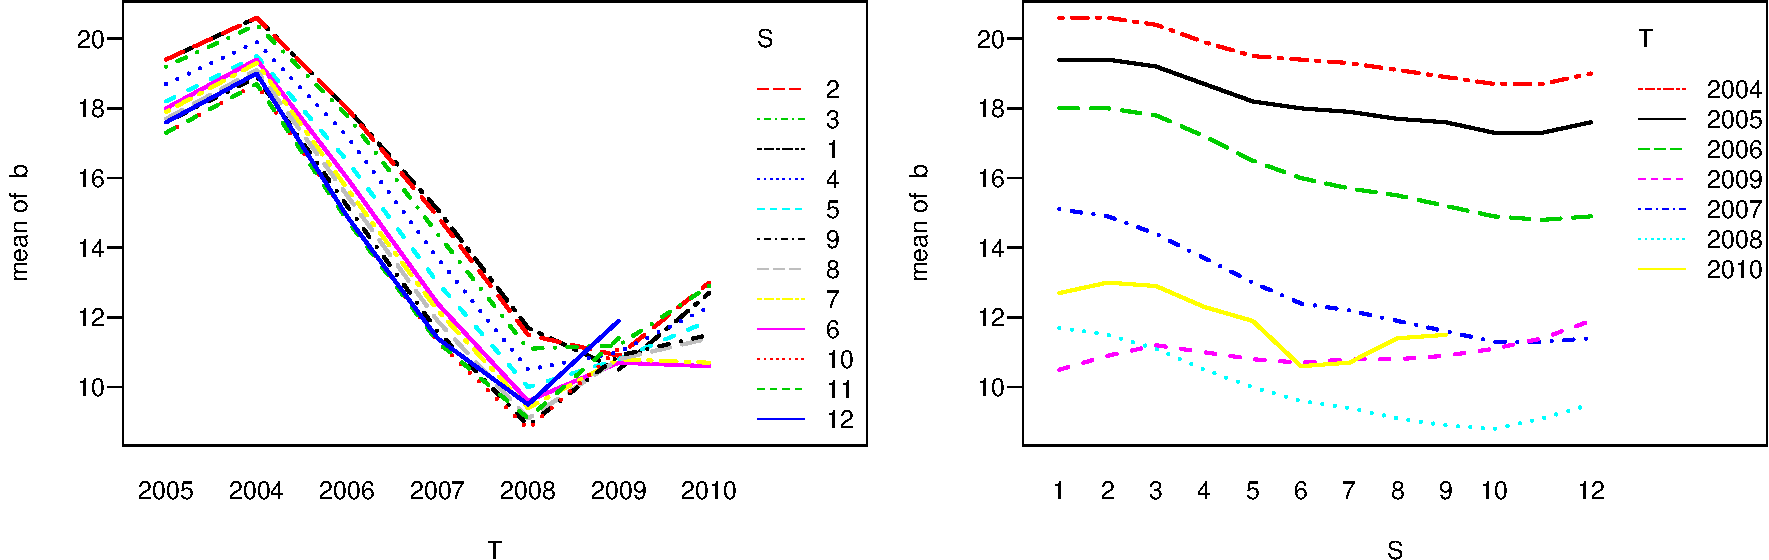
\includegraphics[width=1\linewidth]{NaPrzelajR_files/figure-latex/wy75-1} 

}

\caption{Średnie dla miesięcy i lat.}\label{fig:wy75}
\end{figure}

\hypertarget{part_722}{%
\subsection{Funkcja autokorelacji - ACF}\label{part_722}}

Do identyfikacji składowych szeregu czasowego (trendu oraz sezonowości) można
również wykorzystać funkcję autokorelacji - ACF. W środowisku R jest dostępna
funkcja graficzna \href{https://rdrr.io/github/robjhyndman/forecast/man/tsdisplay.html}{\texttt{forecast::tsdisplay}}, za pomocą której zostają wygenerowane
trzy wykresy: krzywa badanego zjawiska, funkcja autokorelacji ACF oraz funkcja
częściowej autokorelacji PACF.

\begin{Shaded}
\begin{Highlighting}[]
\NormalTok{forecast}\OperatorTok{::}\KeywordTok{tsdisplay}\NormalTok{(b,}\DataTypeTok{col=}\DecValTok{2}\NormalTok{,}\DataTypeTok{lwd=}\DecValTok{2}\NormalTok{,}\DataTypeTok{las=}\DecValTok{1}\NormalTok{)}
\end{Highlighting}
\end{Shaded}

\begin{figure}[h]

{\centering 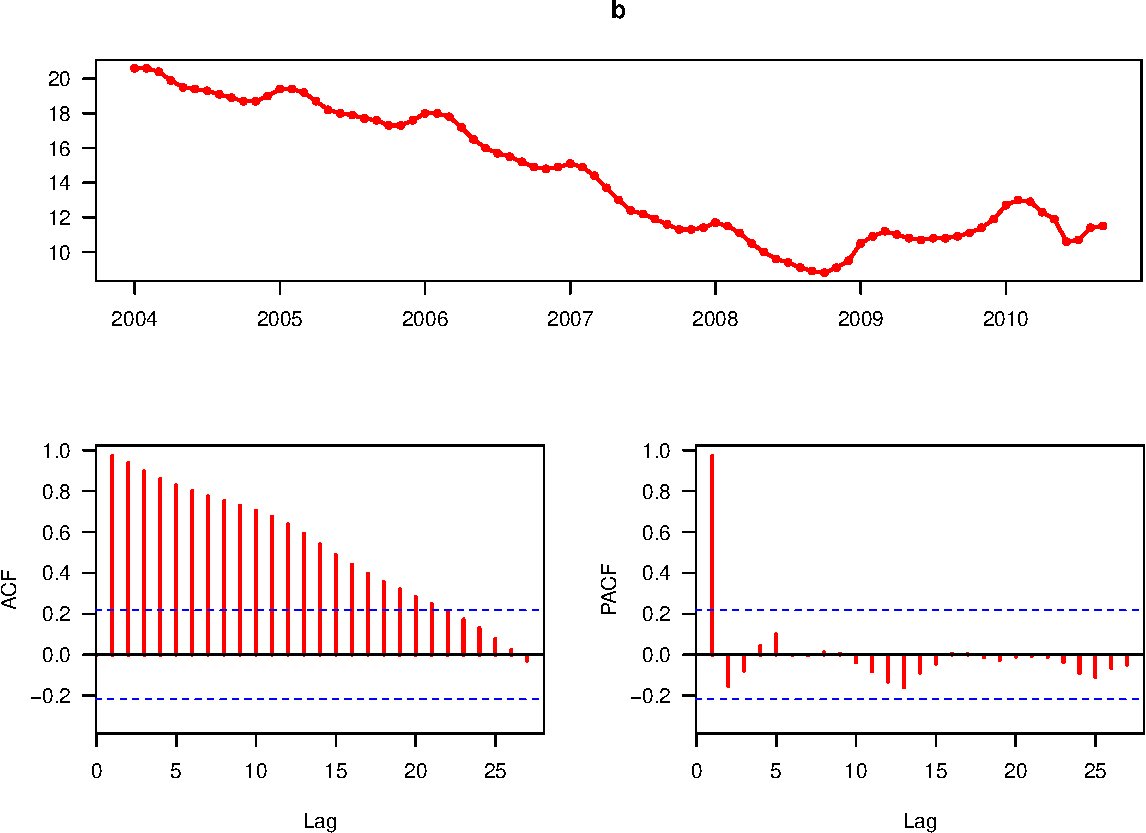
\includegraphics[width=0.7\linewidth]{NaPrzelajR_files/figure-latex/wy76-1} 

}

\caption{Funkcja ACF oraz PACF.}\label{fig:wy76}
\end{figure}

Ponieważ funkcja autokorelacji ACF maleje wykładniczo wraz ze wzrostem parametru \(p\) (rys. \ref{fig:wy76}) należy sądzić, że w badanym procesie występuje trend.

\begin{Shaded}
\begin{Highlighting}[]
\NormalTok{forecast}\OperatorTok{::}\KeywordTok{tsdisplay}\NormalTok{(}\KeywordTok{diff}\NormalTok{(b),}\DataTypeTok{col=}\DecValTok{2}\NormalTok{,}\DataTypeTok{lwd=}\DecValTok{2}\NormalTok{,}\DataTypeTok{las=}\DecValTok{1}\NormalTok{)}
\end{Highlighting}
\end{Shaded}

\begin{figure}[h]

{\centering 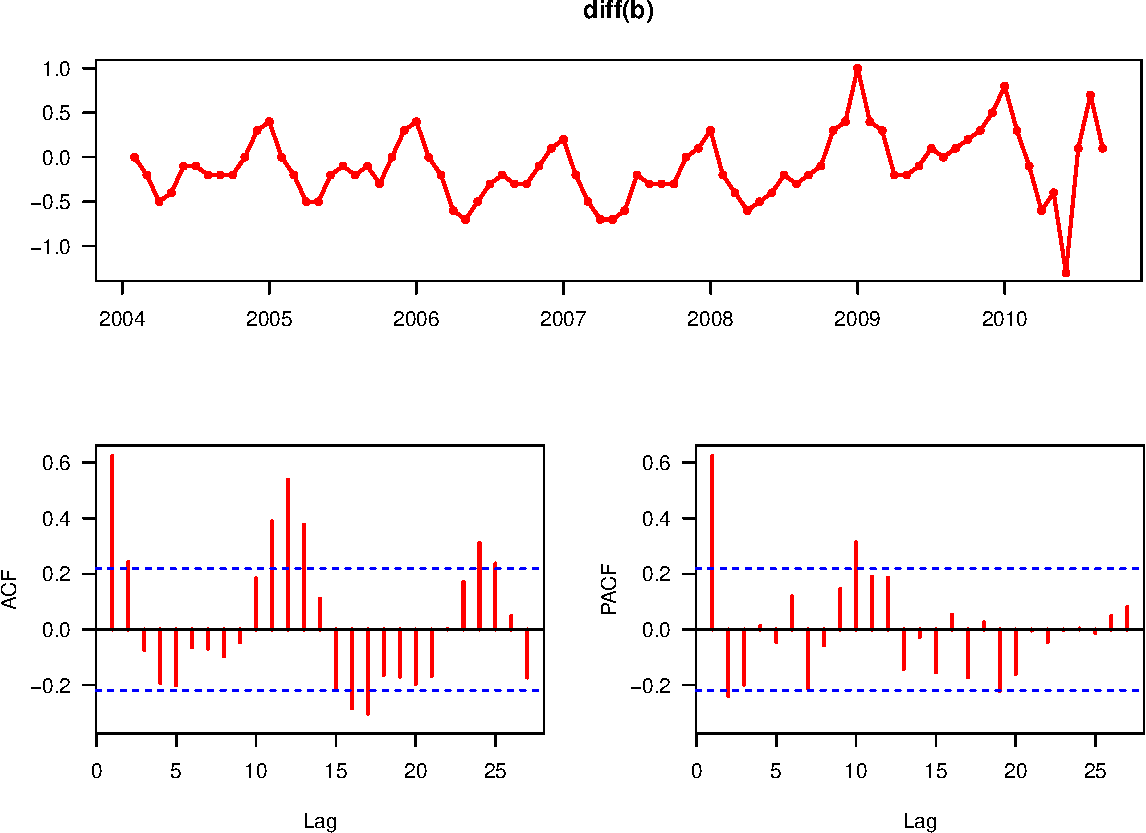
\includegraphics[width=0.7\linewidth]{NaPrzelajR_files/figure-latex/wy77-1} 

}

\caption{Funkcja ACF oraz PACF dla pierwszych różnic.}\label{fig:wy77}
\end{figure}

Po zastosowaniu funkcji różnicowania szeregu czasowego trend został wyeliminowany a funkcja ACF wskazuje na występowanie miesięcznych wahań sezonowych
(rys. \ref{fig:wy77}).

Zatem na podstawie analizy ANOVA oraz funkcji ACF doszliśmy do wniosku,
że badany szereg czasowy charakteryzuje się trendem oraz sezonowością. Również
dzięki funkcji \href{https://rdrr.io/r/stats/stl.html}{\texttt{stl}} za pomocą której dokonaliśmy dekompozycji badanego
procesu (rys. \ref{fig:wy78}) możemy potwierdzić występowanie tendencji rozwojowej oraz
wahań periodycznych.

\begin{Shaded}
\begin{Highlighting}[]
\KeywordTok{plot}\NormalTok{(}\KeywordTok{stl}\NormalTok{(b,}\DataTypeTok{s.window=}\StringTok{"periodic"}\NormalTok{),}\DataTypeTok{col=}\DecValTok{2}\NormalTok{,}\DataTypeTok{lwd=}\DecValTok{2}\NormalTok{)}
\end{Highlighting}
\end{Shaded}

\begin{figure}[h]

{\centering 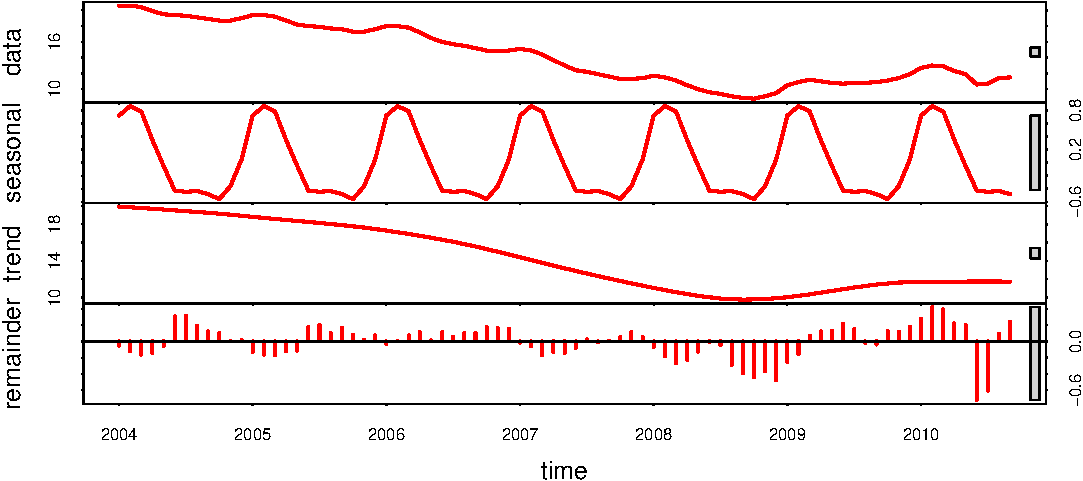
\includegraphics[width=0.7\linewidth]{NaPrzelajR_files/figure-latex/wy78-1} 

}

\caption{Dekompozycja szeregu czasowego.}\label{fig:wy78}
\end{figure}

\hypertarget{part_73}{%
\section{Modele autoregresyjne ARIMA}\label{part_73}}

Modele \(ARIMA\) służą do analizy stacjonarnych szeregów czasowych. W przypadku
gdy szereg jest niestacjonarny należy sprowadzić go do stacjonarności np. poprzez
różnicowanie. W skład modelu \(ARIMA(p, d, q)\) mogą wchodzić następujące elementy:

\begin{itemize}
\item
  \(AR(p)\) -- autoregresja (rząd opóźnienia \(p\))
\item
  \(I(d)\) -- stopień integracji szeregu (krotność różnicowania \(d\))
\item
  \(MA(q)\) -- średnia ruchoma (rząd opóźnienia \(q\))
\end{itemize}

Z kolei gdy w badanym procesie występuje sezonowość należy estymować model o
postaci \(SARIMA(p, d, q)(P, D, Q)_m\) gdzie:

\begin{itemize}
\item
  \(m\) -- sezonowość (np. dla \(m = 4\) sezonowość kwartalna)
\item
  \(P\) -- autoregresja sezonowa
\item
  \(D\) -- integracja sezonowa
\item
  \(Q\) -- średnia ruchoma sezonowa
\end{itemize}

Prawie każdy model \(ARIMA\) można zapisać w dwojaki sposób np dla procesu \(y_t\):

\begin{itemize}
\tightlist
\item
  \(ARIMA(2,0,0)\) czyli \(AR(2)\):
\end{itemize}

\begin{equation}
y_t= \alpha_1 y_{t-1}+\alpha_2 y_{t-2}+\epsilon_t
\label{eq:ar01}
\end{equation}

\begin{itemize}
\tightlist
\item
  \(ARIMA(2,0,1)\) czyli \(ARMA(2,1)\):
\end{itemize}

\begin{equation}
y_t= \alpha_1 y_{t-1}+\alpha_2 y_{t-2}-\beta_1 \epsilon_{t-1}+\epsilon_t
\label{eq:ar02}
\end{equation}

\begin{itemize}
\tightlist
\item
  \(ARIMA(2,1,0)\) czyli \(ARI(2,1)\):
\end{itemize}

\begin{equation}
\Delta y_t= \alpha_1\Delta y_{t-1}+\alpha_2\Delta y_{t-2} +\epsilon_t
\label{eq:ar03}
\end{equation}

\begin{itemize}
\tightlist
\item
  \(SARIMA(1,0,0)(2,0,0)_4\) czyli \(SARI(1)(2)_4\):
\end{itemize}

\begin{equation}
y_t= \alpha_1 y_{t-1}+\alpha_2 y_{t-4}+\alpha_3 y_{t-8} +\epsilon_t
\label{eq:ar04}
\end{equation}

Środowisko R dostarcza wiele funkcji za pomocą których możemy estymować
modele typu \(ARIMA\). Przykładowo komenda \href{https://rdrr.io/r/stats/ar.html}{ar} daje możliwość estymacji modeli autoregresyjnych \(AR(p)\). Opcja method oferuje kilka sposobów szacowania
parametrów modelu: \texttt{burg}, \texttt{ols}, \texttt{mle}, \texttt{yule-walker}, \texttt{yw}. Z kolei funkcja \href{https://rdrr.io/r/stats/arima.html}{\texttt{arima}} służy do estymacji modeli \(ARIMA\) lub \(SARIMA\). Warto także
zwrócić uwagę na pakiet \href{https://rdrr.io/cran/forecast/}{\texttt{forecast}} który dostarcza szereg funkcji do analizy szeregów czasowych.

\hypertarget{part_731}{%
\subsection{Estymacja}\label{part_731}}

Wykorzystując funkcje \href{https://rdrr.io/cran/forecast/man/auto.arima.html}{\texttt{forecast::auto.arima}} proces estymacji modelu \texttt{ARIMA}
przebiega w sposób całkowicie automatyczny. Spośród wielu estymowanych modeli zostaje wybrany ten, który charakteryzuje się najmniejszą wartością kryterium
informacyjnego AIC -- opcja domyślna. W poniższym przykładzie założymy stałą wartość parametru różnicowania \(d=1\).

\begin{Shaded}
\begin{Highlighting}[]
\NormalTok{m <-}\StringTok{ }\NormalTok{forecast}\OperatorTok{::}\KeywordTok{auto.arima}\NormalTok{(b,}\DataTypeTok{d=}\DecValTok{1}\NormalTok{)}
\KeywordTok{summary}\NormalTok{(m)}
\end{Highlighting}
\end{Shaded}

\begin{verbatim}
## Series: b 
## ARIMA(1,1,1)(0,1,0)[12] 
## 
## Coefficients:
##          ar1      ma1
##       0.7948  -0.3710
## s.e.  0.1172   0.1851
## 
## sigma^2 estimated as 0.05246:  log likelihood=4.58
## AIC=-3.16   AICc=-2.78   BIC=3.5
## 
## Training set error measures:
##                       ME      RMSE       MAE       MPE      MAPE
## Training set 0.008136148 0.2067496 0.1162358 0.1296337 0.9846707
##                    MASE       ACF1
## Training set 0.05684101 0.02321908
\end{verbatim}

Oczywiście można samemu założyć liczbę wszystkich parametrów \(p\), \(d\), \(q\), \(P\) , \(D\), \(Q\).

\begin{Shaded}
\begin{Highlighting}[]
\NormalTok{m <-}\StringTok{ }\KeywordTok{arima}\NormalTok{(b,}\DataTypeTok{order=}\KeywordTok{c}\NormalTok{(}\DecValTok{1}\NormalTok{,}\DecValTok{1}\NormalTok{,}\DecValTok{0}\NormalTok{),}\DataTypeTok{seasonal=}\KeywordTok{list}\NormalTok{(}\DataTypeTok{order=}\KeywordTok{c}\NormalTok{(}\DecValTok{1}\NormalTok{,}\DecValTok{0}\NormalTok{,}\DecValTok{0}\NormalTok{),}\DataTypeTok{period=}\DecValTok{12}\NormalTok{))}
\KeywordTok{summary}\NormalTok{(m)}
\end{Highlighting}
\end{Shaded}

\begin{verbatim}
## 
## Call:
## arima(x = b, order = c(1, 1, 0), seasonal = list(order = c(1, 0, 0), period = 12))
## 
## Coefficients:
##          ar1    sar1
##       0.5580  0.7313
## s.e.  0.0912  0.0834
## 
## sigma^2 estimated as 0.04792:  log likelihood = 3.24,  aic = -0.48
## 
## Training set error measures:
##                        ME      RMSE       MAE        MPE     MAPE
## Training set -0.007606623 0.2175572 0.1379808 0.02153749 1.097891
##                   MASE         ACF1
## Training set 0.4505497 -0.006360661
\end{verbatim}

Warto również zaznaczyć, że w programie R mamy możliwość symulowania procesów autoregresji.

\begin{Shaded}
\begin{Highlighting}[]
\NormalTok{y <-}\StringTok{ }\KeywordTok{arima.sim}\NormalTok{( }\DataTypeTok{n=}\DecValTok{1000}\NormalTok{,}
                \DataTypeTok{innov=}\KeywordTok{rnorm}\NormalTok{(}\DecValTok{1000}\NormalTok{,}\DecValTok{0}\NormalTok{,}\DecValTok{2}\NormalTok{), }\CommentTok{# składnik losowy ma rozkład N(0,2)}
                \DataTypeTok{model=}\KeywordTok{list}\NormalTok{(}
                  \DataTypeTok{order =} \KeywordTok{c}\NormalTok{(}\DecValTok{2}\NormalTok{,}\DecValTok{1}\NormalTok{,}\DecValTok{1}\NormalTok{), }\CommentTok{# ilość parametrów}
                  \DataTypeTok{ar =} \KeywordTok{c}\NormalTok{(}\FloatTok{0.3}\NormalTok{, }\FloatTok{0.6}\NormalTok{), }\CommentTok{# wartości parametrów p}
                  \DataTypeTok{ma =} \KeywordTok{c}\NormalTok{( }\FloatTok{0.2}\NormalTok{),     }\CommentTok{# wartości parametrów q}
                  \DataTypeTok{sd =} \KeywordTok{sqrt}\NormalTok{(}\FloatTok{0.1}\NormalTok{)))}
\end{Highlighting}
\end{Shaded}

\begin{Shaded}
\begin{Highlighting}[]
\KeywordTok{par}\NormalTok{(}\DataTypeTok{mar=}\KeywordTok{c}\NormalTok{(}\DecValTok{4}\NormalTok{,}\DecValTok{4}\NormalTok{,}\DecValTok{1}\NormalTok{,}\DecValTok{1}\NormalTok{)}\OperatorTok{+}\FloatTok{0.1}\NormalTok{, }\DataTypeTok{mgp=}\KeywordTok{c}\NormalTok{(}\DecValTok{3}\NormalTok{,}\FloatTok{0.6}\NormalTok{,}\DecValTok{0}\NormalTok{),}\DataTypeTok{las=}\DecValTok{1}\NormalTok{)}
\KeywordTok{plot}\NormalTok{(}\KeywordTok{ts}\NormalTok{(y),}\DataTypeTok{type=}\StringTok{"l"}\NormalTok{,}\DataTypeTok{col=}\StringTok{"SteelBlue"}\NormalTok{)}
\end{Highlighting}
\end{Shaded}

\begin{figure}[h]

{\centering 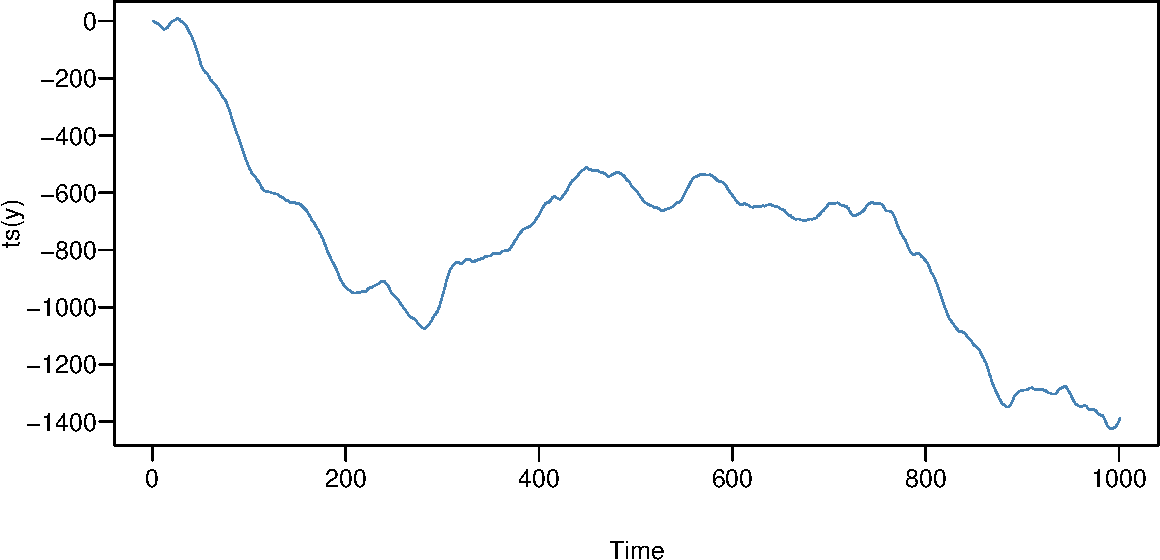
\includegraphics[width=0.7\linewidth]{NaPrzelajR_files/figure-latex/wy79-1} 

}

\caption{Prezentacja graficzna symulowanego procesu.}\label{fig:wy79}
\end{figure}

\begin{Shaded}
\begin{Highlighting}[]
\NormalTok{s <-}\StringTok{ }\KeywordTok{arima}\NormalTok{(y,}\DataTypeTok{order=}\KeywordTok{c}\NormalTok{(}\DecValTok{2}\NormalTok{,}\DecValTok{1}\NormalTok{,}\DecValTok{1}\NormalTok{))}
\NormalTok{s}
\end{Highlighting}
\end{Shaded}

\begin{verbatim}
## 
## Call:
## arima(x = y, order = c(2, 1, 1))
## 
## Coefficients:
##          ar1     ar2     ma1
##       0.3721  0.5508  0.1155
## s.e.  0.0542  0.0486  0.0644
## 
## sigma^2 estimated as 3.975:  log likelihood = -2109.99,  aic = 4227.97
\end{verbatim}

Dzięki zastosowaniu funkcji \href{https://rdrr.io/cran/forecast/man/ndiffs.html}{\texttt{forecast::ndiffs}} mamy możliwość sprawdzenia czy rzeczywiście proces y jest zintegrowany w stopniu pierwszym tzn. \(I(1)\). Za pomocą opcji test możemy wybrać procedurę z jakiej chcemy skorzystać: \texttt{pp} -- test Phillipsa-Perrona, \texttt{adf} -- test Dickeya-Fullera lub \texttt{kpss} -- test Kwiatkowski-Phillips-Schmidt-Shin. Poziom istotności \texttt{alpha} także możemy zmieniać.

\begin{Shaded}
\begin{Highlighting}[]
\NormalTok{forecast}\OperatorTok{::}\KeywordTok{ndiffs}\NormalTok{(y,}\DataTypeTok{test=}\StringTok{"pp"}\NormalTok{,}\DataTypeTok{alpha=}\FloatTok{0.05}\NormalTok{)}
\end{Highlighting}
\end{Shaded}

\begin{verbatim}
## [1] 1
\end{verbatim}

Wynikiem funkcji \href{https://rdrr.io/cran/forecast/man/ndiffs.html}{\texttt{forecast::ndiffs}} zawsze jest stopień zintegrowania badanego
procesu. Zatem należy stwierdzić, że w zmiennej \(y\) występuje pierwiastek jednostkowy \(d = 1\).

\hypertarget{part_732}{%
\subsection{Weryfikacja}\label{part_732}}

Etap weryfikacji oszacowanego modelu \(ARIMA\) polega na sprawdzeniu hipotezy zerowej o braku zjawiska autokorelacji w procesie reszt. Do tego celu możemy wykorzystać test Ljunga-Boxa.

\begin{Shaded}
\begin{Highlighting}[]
\NormalTok{r <-}\StringTok{ }\KeywordTok{resid}\NormalTok{(m)}
\NormalTok{p <-}\StringTok{ }\KeywordTok{sapply}\NormalTok{(}\DecValTok{1}\OperatorTok{:}\DecValTok{10}\NormalTok{,}\ControlFlowTok{function}\NormalTok{(i) }\KeywordTok{Box.test}\NormalTok{(r, i, }\DataTypeTok{type =} \StringTok{"Ljung-Box"}\NormalTok{)}\OperatorTok{$}\NormalTok{p.value)}
\NormalTok{p}
\end{Highlighting}
\end{Shaded}

\begin{verbatim}
##  [1] 0.9535022 0.9152975 0.5318782 0.6333194 0.7667281 0.8522917 0.8863058
##  [8] 0.9348725 0.9625130 0.9775571
\end{verbatim}

Tak więc na podstawie testu Ljunga-Boxa brak jest podstaw do odrzucenia hipotezy
zerowej zakładającej brak autokorelacji. Wniosek ten potwierdzają również wykresy
wykonane za pomocą komendy \href{https://rdrr.io/r/stats/tsdiag.html}{\texttt{tsdiag}} (rys. \ref{fig:wy80}).

\begin{Shaded}
\begin{Highlighting}[]
\KeywordTok{par}\NormalTok{(}\DataTypeTok{mar=}\KeywordTok{c}\NormalTok{(}\DecValTok{4}\NormalTok{,}\DecValTok{4}\NormalTok{,}\DecValTok{1}\NormalTok{,}\DecValTok{1}\NormalTok{)}\OperatorTok{+}\FloatTok{0.1}\NormalTok{, }\DataTypeTok{mgp=}\KeywordTok{c}\NormalTok{(}\DecValTok{3}\NormalTok{,}\FloatTok{0.6}\NormalTok{,}\DecValTok{0}\NormalTok{),}\DataTypeTok{las=}\DecValTok{1}\NormalTok{)}
\KeywordTok{tsdiag}\NormalTok{(m)}
\end{Highlighting}
\end{Shaded}

\begin{figure}[h]

{\centering 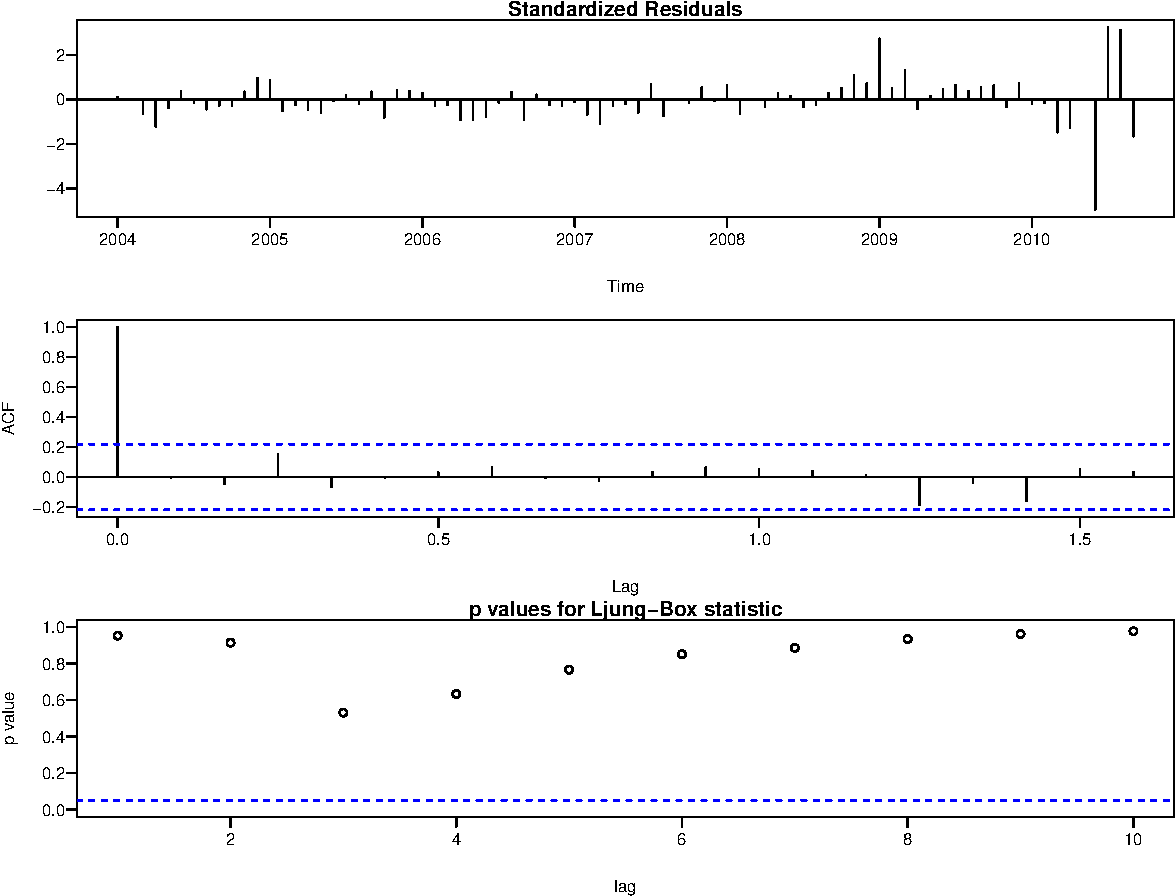
\includegraphics[width=0.7\linewidth]{NaPrzelajR_files/figure-latex/wy80-1} 

}

\caption{Diagnostyka reszt modelu.}\label{fig:wy80}
\end{figure}

\hypertarget{part_733}{%
\subsection{Prognozowanie}\label{part_733}}

Funkcja \href{https://rdrr.io/cran/forecast/man/forecast.html}{\texttt{forecast::forecast}} służy do obliczania prognoz na podstawie danego
modelu. W naszym przykładzie liczbę okresów do prognozowania została ustalona
na \(12\) miesięcy. Natomiast przedziały predykcji zostały ustalone na poziomie 80\%
i \(95\%\) -- są to wartości domyślne. Gdybyśmy chcieli je zmienić na \(99\%\) wystarczy użyć polecenia \texttt{level=99}.

\begin{Shaded}
\begin{Highlighting}[]
\NormalTok{forecast}\OperatorTok{::}\KeywordTok{forecast}\NormalTok{(m,}\DataTypeTok{h=}\DecValTok{12}\NormalTok{)}
\end{Highlighting}
\end{Shaded}

\begin{verbatim}
##          Point Forecast     Lo 80    Hi 80     Lo 95    Hi 95
## Oct 2010       11.66125 11.380716 11.94178 11.232211 12.09029
## Nov 2010       11.88899 11.369636 12.40835 11.094703 12.68329
## Dec 2010       12.25929 11.521215 12.99738 11.130499 13.38809
## Jan 2011       12.84691 11.912406 13.78141 11.417711 14.27611
## Feb 2011       13.06774 11.956998 14.17848 11.369006 14.76648
## Mar 2011       12.99543 11.725520 14.26533 11.053272 14.93758
## Apr 2011       12.55712 11.142176 13.97207 10.393148 14.72110
## May 2011       12.26487 10.716515 13.81323  9.896864 14.63288
## Jun 2011       11.31437  9.642230 12.98652  8.757050 13.87170
## Jul 2011       11.38758  9.599679 13.17548  8.653222 14.12194
## Aug 2011       11.89950 10.002628 13.79638  8.998482 14.80053
## Sep 2011       11.97266  9.972585 13.97273  8.913812 15.03150
\end{verbatim}

\begin{Shaded}
\begin{Highlighting}[]
\KeywordTok{par}\NormalTok{(}\DataTypeTok{mar=}\KeywordTok{c}\NormalTok{(}\DecValTok{4}\NormalTok{,}\DecValTok{4}\NormalTok{,}\DecValTok{1}\NormalTok{,}\DecValTok{1}\NormalTok{)}\OperatorTok{+}\FloatTok{0.1}\NormalTok{, }\DataTypeTok{mgp=}\KeywordTok{c}\NormalTok{(}\DecValTok{3}\NormalTok{,}\FloatTok{0.6}\NormalTok{,}\DecValTok{0}\NormalTok{),}\DataTypeTok{las=}\DecValTok{1}\NormalTok{)}
\KeywordTok{plot}\NormalTok{(forecast}\OperatorTok{::}\KeywordTok{forecast}\NormalTok{(m,}\DataTypeTok{h=}\DecValTok{12}\NormalTok{))}
\end{Highlighting}
\end{Shaded}

\begin{figure}[h]

{\centering 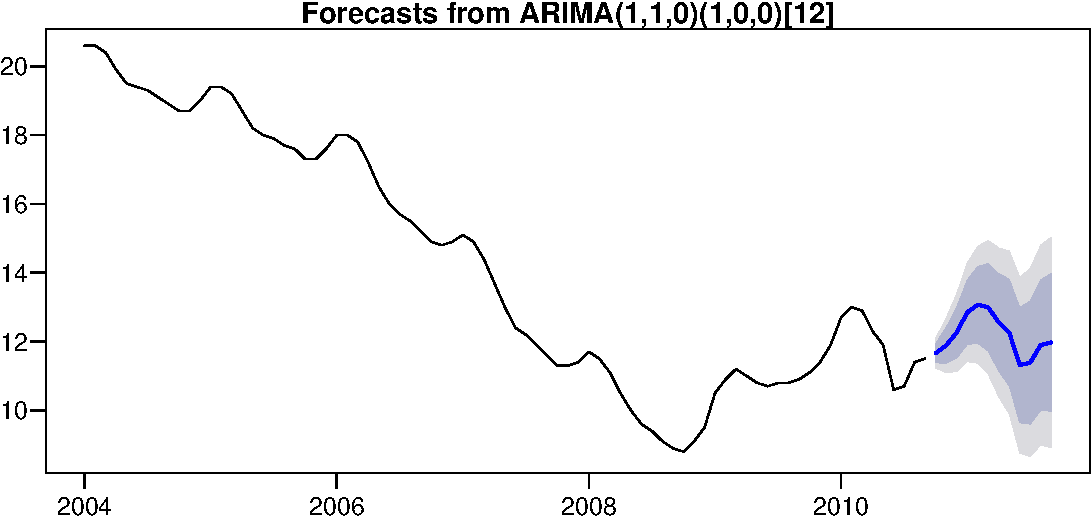
\includegraphics[width=0.7\linewidth]{NaPrzelajR_files/figure-latex/wy81-1} 

}

\caption{Prognoza stopy bezrobocia od 10.2010–09.2011.}\label{fig:wy81}
\end{figure}

Dodatkowo możemy wyznaczyć błędy prognoz za pomocą funkcji \href{https://rdrr.io/r/stats/predict.lm.html}{\texttt{predict}}:

\begin{Shaded}
\begin{Highlighting}[]
\NormalTok{p <-}\StringTok{ }\KeywordTok{predict}\NormalTok{(m,}\DataTypeTok{n.ahead=}\DecValTok{12}\NormalTok{)}
\KeywordTok{ts}\NormalTok{( }\KeywordTok{cbind}\NormalTok{(}\DataTypeTok{pred=}\NormalTok{p}\OperatorTok{$}\NormalTok{pred, }\DataTypeTok{se=}\NormalTok{p}\OperatorTok{$}\NormalTok{se, }\DataTypeTok{error=}\NormalTok{p}\OperatorTok{$}\NormalTok{se}\OperatorTok{/}\NormalTok{p}\OperatorTok{$}\NormalTok{pred), }\DataTypeTok{start=}\KeywordTok{c}\NormalTok{(}\DecValTok{2010}\NormalTok{,}\DecValTok{10}\NormalTok{),}\DataTypeTok{freq=}\DecValTok{12}\NormalTok{)}
\end{Highlighting}
\end{Shaded}

\begin{verbatim}
##              pred        se      error
## Oct 2010 11.66125 0.2189006 0.01877162
## Nov 2010 11.88899 0.4052582 0.03408683
## Dec 2010 12.25929 0.5759270 0.04697881
## Jan 2011 12.84691 0.7291963 0.05676045
## Feb 2011 13.06774 0.8667176 0.06632497
## Mar 2011 12.99543 0.9909135 0.07625094
## Apr 2011 12.55712 1.1040891 0.08792532
## May 2011 12.26487 1.2081893 0.09850810
## Jun 2011 11.31437 1.3047811 0.11532066
## Jul 2011 11.38758 1.3951054 0.12251115
## Aug 2011 11.89950 1.4801411 0.12438678
## Sep 2011 11.97266 1.5606634 0.13035232
\end{verbatim}

Otrzymane wartości prognostyczne wskazują, iż należy się spodziewać wzrostu stopy
bezrobocia od października \(2010\)--\(11,66\%\) do lutego 2011--\(13,07\%\). Od marca
należy się spodziewać spadku tego wskaźnika do poziomu \(11,31\%\) w czerwcu \(2011\)
roku. Następnie będzie on znów powoli wzrastał i w miesiącu wrześniu osiągnie
wartość \(11,97\%\). Należy także zwrócic uwagę na oszacowane błędy otrzymanych
prognoz. Dla października 2010 wyniósł on \(1,9\%\) i cały czas wzrastał, aż do poziomu \(13,04\%\) dla września \(2011\) roku.

\hypertarget{part_74}{%
\section{Modele adaptacyjne}\label{part_74}}

\hypertarget{part_741}{%
\subsection{Estymacja}\label{part_741}}

Podobnie jak w przypadku modelu \(ARIMA\) także estymacja modelu adaptacyjnego
może przebiegać w sposób całkowicie automatyczny. Wykorzystamy do tego celu
funkcje \href{https://rdrr.io/cran/forecast/man/ets.html}{\texttt{forecast::ets}}.

\begin{Shaded}
\begin{Highlighting}[]
\NormalTok{n <-}\StringTok{ }\NormalTok{forecast}\OperatorTok{::}\KeywordTok{ets}\NormalTok{(b,}\DataTypeTok{model=}\StringTok{"ZZZ"}\NormalTok{,}\DataTypeTok{damped=}\OtherTok{NULL}\NormalTok{)}
\KeywordTok{summary}\NormalTok{(n)}
\end{Highlighting}
\end{Shaded}

\begin{verbatim}
## ETS(A,Ad,A) 
## 
## Call:
##  forecast::ets(y = b, model = "ZZZ", damped = NULL) 
## 
##   Smoothing parameters:
##     alpha = 0.9978 
##     beta  = 0.132 
##     gamma = 0.0016 
##     phi   = 0.9752 
## 
##   Initial states:
##     l = 19.8288 
##     b = -0.0952 
##     s = 0.0294 -0.3797 -0.5833 -0.4821 -0.3923 -0.3453
##            -0.3235 -0.0403 0.3291 0.7522 0.7916 0.6442
## 
##   sigma:  0.2251
## 
##      AIC     AICc      BIC 
## 131.2611 142.2934 174.3612 
## 
## Training set error measures:
##                        ME     RMSE       MAE        MPE     MAPE
## Training set -0.003431383 0.200049 0.1258755 0.05990526 1.004237
##                    MASE      ACF1
## Training set 0.06155499 0.2850916
\end{verbatim}

\begin{Shaded}
\begin{Highlighting}[]
\KeywordTok{logLik}\NormalTok{(n) }\CommentTok{# logarytm wiarygodności}
\end{Highlighting}
\end{Shaded}

\begin{verbatim}
## 'log Lik.' -47.63055 (df=18)
\end{verbatim}

Spośród wszystkich modeli, które były estymowane -- \texttt{model="ZZZ"} z wykorzystaniem optymalizacji logarytmu wiarygodności -- \texttt{opt.crit="lik"}, został wybrany
model o najmniejszym kryterium informacyjnym AIC -- \texttt{ic="aic"}. Dostępne są
także inne metody optymalizacyjne do szacowania parametrów: \texttt{mse}, \texttt{amse}, \texttt{nmse},
\texttt{sigma}. Także wybór kryterium informacyjnego (za pomocą którego dokonujemy
wyboru najlepszego modelu) możemy wybrać samodzielnie: \texttt{aic}, \texttt{aicc}, \texttt{bic}. Tak
przeprowadzona estymacja doprowadziła do otrzymania modelu \texttt{"AAdA"}, który charakteryzuje się następującymi cechami: \texttt{A} -- addytywny składnik losowy (pierwsza
litera), \texttt{Ad} -- trend addytywny (druga litera), gdzie mała litera d oznacza, że została wybrana również opcja \texttt{damped=T} czyli ``przygaszenie'' trendu, \texttt{A} -- addytywne
wachania sezonowe (trzecia litera). Zatem otrzymaliśmy model Wintersa z addytywnymi wahaniami periodycznymi:

\begin{Shaded}
\begin{Highlighting}[]
\NormalTok{n <-}\StringTok{ }\NormalTok{forecast}\OperatorTok{::}\KeywordTok{ets}\NormalTok{(b, }\DataTypeTok{model=}\StringTok{"AAA"}\NormalTok{)}
\NormalTok{n}
\end{Highlighting}
\end{Shaded}

\begin{verbatim}
## ETS(A,Ad,A) 
## 
## Call:
##  forecast::ets(y = b, model = "AAA") 
## 
##   Smoothing parameters:
##     alpha = 0.9978 
##     beta  = 0.132 
##     gamma = 0.0016 
##     phi   = 0.9752 
## 
##   Initial states:
##     l = 19.8288 
##     b = -0.0952 
##     s = 0.0294 -0.3797 -0.5833 -0.4821 -0.3923 -0.3453
##            -0.3235 -0.0403 0.3291 0.7522 0.7916 0.6442
## 
##   sigma:  0.2251
## 
##      AIC     AICc      BIC 
## 131.2611 142.2934 174.3612
\end{verbatim}

Oczywiście korzystając z funkcji \href{https://rdrr.io/cran/forecast/man/ets.html}{\texttt{forecast::ets}} oraz opcji \texttt{model} możemy od razu zawęzić
grupę modeli, spośród których zostanie wybrany najlepszy z nich: modele Browna
-- \texttt{model="ZNN"}, modele Browna lub Holta -- \texttt{model="ZZN"}, modele Browna, Holta
lub Wintersa -- \texttt{model="ZZZ"}. Jest również możliwość estymacji modeli o ustalonych
parametrach: \texttt{alpha}, \texttt{beta}, \texttt{gamma}, \texttt{phi}. Natomiast gdy ich wartości zawierają się
w pewnych przedziałach liczbowych, przykładowo jeśli \(\alpha = (0,11 - 0,53)\), \(\beta = (0,41 - 0,68)\) i \(\gamma = (0,65 - 0,78)\) to należy użyć opcji \texttt{level=c(0.11,0.41,0.65)} oraz \texttt{upper=c(0.53,0.68,0.78)}.

\hypertarget{part_742}{%
\subsection{Prognozowanie}\label{part_742}}

Do procesu prognozowania z wykorzystaniem modelu adaptacyjnego możemy również wykorzystać funkcję \href{https://rdrr.io/cran/forecast/man/forecast.html}{\texttt{forecast::forecast}}.

\begin{Shaded}
\begin{Highlighting}[]
\NormalTok{forecast}\OperatorTok{::}\KeywordTok{forecast}\NormalTok{(n,}\DataTypeTok{h=}\DecValTok{12}\NormalTok{)}
\end{Highlighting}
\end{Shaded}

\begin{verbatim}
##          Point Forecast    Lo 80    Hi 80     Lo 95    Hi 95
## Oct 2010       11.45805 11.16963 11.74646 11.016945 11.89914
## Nov 2010       11.71903 11.28458 12.15348 11.054594 12.38346
## Dec 2010       12.18460 11.61967 12.74953 11.320617 13.04858
## Jan 2011       12.85520 12.16506 13.54533 11.799728 13.91066
## Feb 2011       13.05585 12.24227 13.86942 11.811592 14.30010
## Mar 2011       13.06843 12.13164 14.00522 11.635734 14.50113
## Apr 2011       12.69693 11.63640 13.75747 11.074992 14.31888
## May 2011       12.37728 11.19211 13.56246 10.564716 14.18985
## Jun 2011       12.14212 10.83122 13.45302 10.137273 14.14697
## Jul 2011       12.16889 10.73111 13.60667  9.969991 14.36778
## Aug 2011       12.16869 10.60287 13.73452  9.773968 14.56341
## Sep 2011       12.12366 10.42866 13.81867  9.531375 14.71595
\end{verbatim}

\begin{Shaded}
\begin{Highlighting}[]
\KeywordTok{par}\NormalTok{(}\DataTypeTok{mar=}\KeywordTok{c}\NormalTok{(}\DecValTok{4}\NormalTok{,}\DecValTok{4}\NormalTok{,}\DecValTok{1}\NormalTok{,}\DecValTok{1}\NormalTok{)}\OperatorTok{+}\FloatTok{0.1}\NormalTok{, }\DataTypeTok{mgp=}\KeywordTok{c}\NormalTok{(}\DecValTok{3}\NormalTok{,}\FloatTok{0.6}\NormalTok{,}\DecValTok{0}\NormalTok{),}\DataTypeTok{las=}\DecValTok{1}\NormalTok{)}
\KeywordTok{plot}\NormalTok{(forecast}\OperatorTok{::}\KeywordTok{forecast}\NormalTok{(n,}\DataTypeTok{h=}\DecValTok{12}\NormalTok{))}
\end{Highlighting}
\end{Shaded}

\begin{figure}[h]

{\centering 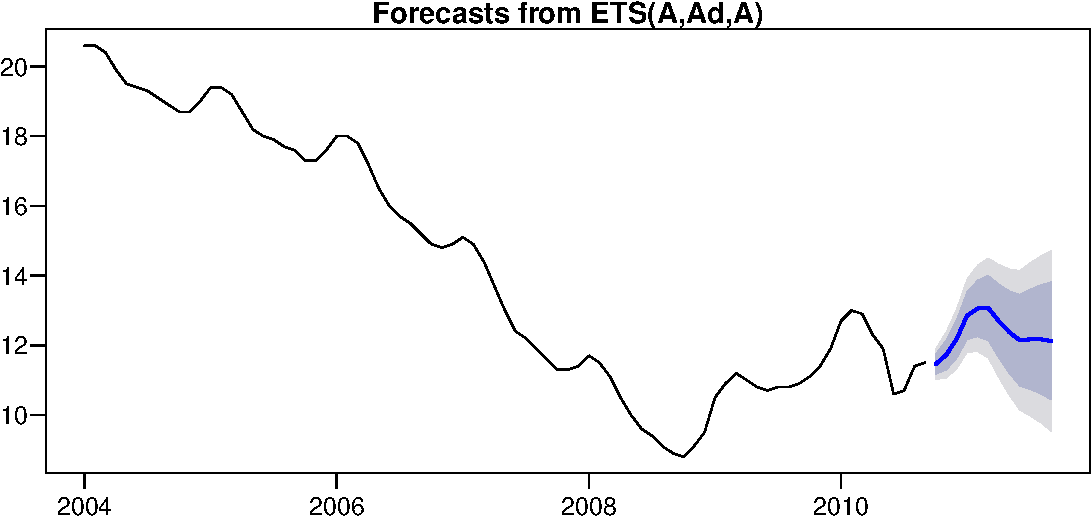
\includegraphics[width=0.7\linewidth]{NaPrzelajR_files/figure-latex/wy82-1} 

}

\caption{Prognoza stopy bezrobocia od 10.2010–09.2011.}\label{fig:wy82}
\end{figure}

W przypadku gdy wykonaliśmy dwie prognozy za pomocą różnych modeli (np.
modelu \(ARIMA\) i adaptacyjnego) warto skorzystać z testu Diebold-Mariano. Hipoteza zerowa tego tesu zakłada, że dokładność predykcyjna dwóch modeli jest jednakowa. Założenie \texttt{alt="two.sided"} (test dwustronny) jest opcją domyślną, możemy
ją zmienić dodając polecenie \texttt{alt="g"} (test prawostronny) lub \texttt{alt="l"} (test lewostronny).

\begin{Shaded}
\begin{Highlighting}[]
\NormalTok{forecast}\OperatorTok{::}\KeywordTok{dm.test}\NormalTok{(}\KeywordTok{resid}\NormalTok{(m),}\KeywordTok{resid}\NormalTok{(n))}
\end{Highlighting}
\end{Shaded}

\begin{verbatim}
## 
##  Diebold-Mariano Test
## 
## data:  resid(m)resid(n)
## DM = 1.0538, Forecast horizon = 1, Loss function power = 2,
## p-value = 0.2951
## alternative hypothesis: two.sided
\end{verbatim}

\hypertarget{part_8}{%
\chapter{Przykład analizy tabel wielodzielczych}\label{part_8}}

\begin{center}\rule{0.5\linewidth}{\linethickness}\end{center}

\hypertarget{part_81}{%
\section{Wprowadzenie}\label{part_81}}

Zbiór danych, który zostanie wykorzystany do przeprowadzenia analiz jest dostępny
pod nazwą \href{https://rdrr.io/r/datasets/Titanic.html}{\texttt{Titanic}}. Zawiera on informacje na temat losu 2201 pasażerów
oceanicznego liniowca ``Titanic''. Do dyspozycji mamy cztery zmienne nominalne:

\begin{itemize}
\item
  \textbf{Class} -- klasy podróżowania: 1st (pierwsza), 2nd (druga), 3rd (trzecia), Crew
  (załoga),
\item
  \textbf{Sex} -- płeć: Male (mężczyzna), Female (kobieta),
\item
  \textbf{Age} -- wiek: Adult (dorosły), Child (dziecko),
\item
  \textbf{Survived} -- przeżycie: No (nie), Yes (tak).
\end{itemize}

Oryginalny zestaw danych (wielowymiarowa tabela kontyngencji) został przekształcony o nazwie \texttt{t}. Fragment naszych
danych jest widoczny poniżej:

\begin{Shaded}
\begin{Highlighting}[]
\NormalTok{t <-}\StringTok{ }\NormalTok{DescTools}\OperatorTok{::}\KeywordTok{Untable}\NormalTok{(Titanic)}
\NormalTok{t[}\DecValTok{1}\OperatorTok{:}\DecValTok{3}\NormalTok{,]}
\end{Highlighting}
\end{Shaded}

\begin{verbatim}
##   Class  Sex   Age Survived
## 1   3rd Male Child       No
## 2   3rd Male Child       No
## 3   3rd Male Child       No
\end{verbatim}

Celem naszych badań będzie próba opisu zależności między przeżyciem, a klasą
podróżowania, płcią podróżnych oraz ich wiekiem.

\hypertarget{part_82}{%
\section{Test chi-kwadrat}\label{part_82}}

Do analizy zależności między dwiema zmiennymi zostanie wykorzystamy test \(\chi^2\). W
pakiecie R jest dostępna funkcja \href{}{\texttt{assocstats::vcd}} za pomocą której wykonywane
są dwa testy badające niezależność: test \(\chi^2\) oraz test \(G\):

\begin{subequations}
\begin{align}
\chi^2=\sum_{i=1}^{r} \sum_{j=1}^{c}\frac{(O_{ij}-E_{ij})^2}{E_{ij}} \label{eq:wz81}\\
G=2\sum_{i}^{r}\sum_{j=1}^{c} O_{ij}\ln\left(\frac{O_{ij}}{E_{ij}}\right) \label{eq:wz82}
\end{align}
\end{subequations}

gdzie:

\begin{itemize}
\item
  \(r\) -- liczba wierszy,
\item
  \(c\) -- liczba kolumn,
\item
  \(O_{ij}\) -- empiryczna liczebność \(i\)-tego wiersza oraz \(j\)-tej kolumny,
\item
  \(E_{ij}\) -- oczekiwana liczebność \(i\)-tego wiersza oraz \(j\)-tej kolumny.
\end{itemize}

Dodatkowo podawane są również współczynniki korelacji: \(\phi\)-Yula, \(V\)-Pearsona i \(V\)-Cramera. A zatem spróbujmy odpowiedzieć na następujące pytania:

\begin{enumerate}
\def\labelenumi{\arabic{enumi}.}
\tightlist
\item
  Czy na przeżycie katastrofy miała wpływ płeć?
\end{enumerate}

\begin{Shaded}
\begin{Highlighting}[]
\CommentTok{# tablica kontygencji:}
\NormalTok{s <-}\StringTok{ }\KeywordTok{xtabs}\NormalTok{(}\OperatorTok{~}\NormalTok{Survived}\OperatorTok{+}\NormalTok{Sex, }\DataTypeTok{data=}\NormalTok{t) }
\NormalTok{gplots}\OperatorTok{::}\KeywordTok{balloonplot}\NormalTok{(s,}\DataTypeTok{dotcolor=}\StringTok{"gray80"}\NormalTok{)}
\end{Highlighting}
\end{Shaded}

\begin{figure}[h]

{\centering 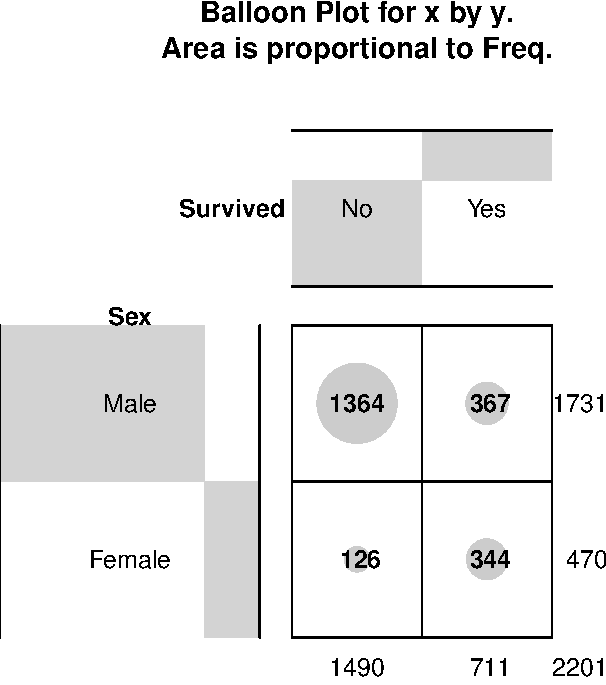
\includegraphics[width=0.4\linewidth]{NaPrzelajR_files/figure-latex/wy81A-1} 

}

\caption{Przeżycie i płeć.}\label{fig:wy81A}
\end{figure}

\begin{Shaded}
\begin{Highlighting}[]
\NormalTok{vcd}\OperatorTok{::}\KeywordTok{assocstats}\NormalTok{(s)}
\end{Highlighting}
\end{Shaded}

\begin{verbatim}
##                     X^2 df P(> X^2)
## Likelihood Ratio 434.47  1        0
## Pearson          456.87  1        0
## 
## Phi-Coefficient   : 0.456 
## Contingency Coeff.: 0.415 
## Cramer's V        : 0.456
\end{verbatim}

Na podstawie testu \(\chi^2\) oraz wykresu (rys. \ref{fig:wy81A}) możemy wnioskować, że występuje istotne powiązanie między przeżyciem katastrofy, a płcią pasażerów (p-value= 0, \(V = 0,456\)).

\begin{Shaded}
\begin{Highlighting}[]
\NormalTok{ps <-}\StringTok{ }\KeywordTok{prop.table}\NormalTok{(s,}\DecValTok{2}\NormalTok{);ps}
\end{Highlighting}
\end{Shaded}

\begin{verbatim}
##         Sex
## Survived      Male    Female
##      No  0.7879838 0.2680851
##      Yes 0.2120162 0.7319149
\end{verbatim}

Obliczenia procentowe wskazują, że przeżyło \(73\%\) kobiet oraz tylko \(21\%\) mężczyzn.

\begin{Shaded}
\begin{Highlighting}[]
\NormalTok{ns<-ps}\OperatorTok{/}\NormalTok{(}\DecValTok{1}\OperatorTok{-}\NormalTok{ps);ns }\CommentTok{# szanse przeżycia}
\end{Highlighting}
\end{Shaded}

\begin{verbatim}
##         Sex
## Survived      Male    Female
##      No  3.7166213 0.3662791
##      Yes 0.2690616 2.7301587
\end{verbatim}

\begin{Shaded}
\begin{Highlighting}[]
\NormalTok{ns[,}\DecValTok{1}\NormalTok{]}\OperatorTok{/}\NormalTok{ns[,}\DecValTok{2}\NormalTok{]    }\CommentTok{# ilorazy szans przeżycia}
\end{Highlighting}
\end{Shaded}

\begin{verbatim}
##          No         Yes 
## 10.14696596  0.09855163
\end{verbatim}

Obliczony iloraz szans \(OR = 10,15\) wskazuje, że szansa przeżycia katastrofy na Titanicu wśród kobiet \((2,7301587)\) była ponad dziesięć razy większa niż wśród mężczyzn \((0,2690616)\).

\begin{enumerate}
\def\labelenumi{\arabic{enumi}.}
\setcounter{enumi}{1}
\tightlist
\item
  Czy na przeżycie katastrofy miała wpływ klasa w której podróżowano?
\end{enumerate}

\begin{Shaded}
\begin{Highlighting}[]
\NormalTok{c <-}\StringTok{ }\KeywordTok{xtabs}\NormalTok{(}\OperatorTok{~}\NormalTok{Survived}\OperatorTok{+}\NormalTok{Class,}\DataTypeTok{data=}\NormalTok{t) }\CommentTok{# tablica kontygencji}
\NormalTok{gplots}\OperatorTok{::}\KeywordTok{balloonplot}\NormalTok{(c,}\DataTypeTok{dotcolor=}\StringTok{"gray80"}\NormalTok{)}
\end{Highlighting}
\end{Shaded}

\begin{figure}[h]

{\centering 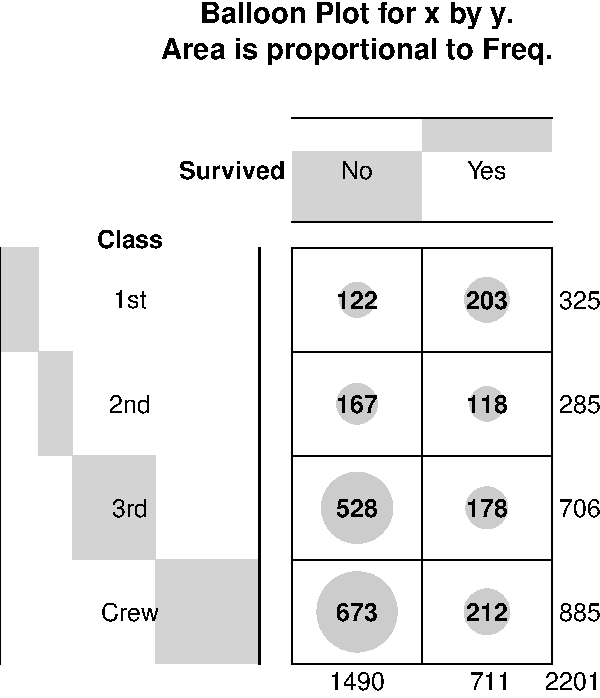
\includegraphics[width=0.4\linewidth]{NaPrzelajR_files/figure-latex/wy82A-1} 

}

\caption{Przeżycie i klasa podróżowania.}\label{fig:wy82A}
\end{figure}

\begin{Shaded}
\begin{Highlighting}[]
\NormalTok{vcd}\OperatorTok{::}\KeywordTok{assocstats}\NormalTok{(c)}
\end{Highlighting}
\end{Shaded}

\begin{verbatim}
##                    X^2 df P(> X^2)
## Likelihood Ratio 180.9  3        0
## Pearson          190.4  3        0
## 
## Phi-Coefficient   : NA 
## Contingency Coeff.: 0.282 
## Cramer's V        : 0.294
\end{verbatim}

Ponieważ p-value = 0 to należy sądzić, że istnieje zależność między przeżyciem a
klasą w której podróżowali uczestnicy rejsu. O wysokim powiązaniu tych zmiennych
świdczy także wysoki współczynnik korelacji \(V = 0,29\). Dodajmy, że współczynnik zależności \(\phi\) jest obliczany tylko dla tabel kontyngencji \(2\times2\).

\begin{Shaded}
\begin{Highlighting}[]
\NormalTok{pc <-}\StringTok{ }\KeywordTok{prop.table}\NormalTok{(c,}\DecValTok{2}\NormalTok{);pc}
\end{Highlighting}
\end{Shaded}

\begin{verbatim}
##         Class
## Survived       1st       2nd       3rd      Crew
##      No  0.3753846 0.5859649 0.7478754 0.7604520
##      Yes 0.6246154 0.4140351 0.2521246 0.2395480
\end{verbatim}

Po obliczeniu wartości procentowych dochodzimy do wniosku, że najwięcej przeżyło
tych osób, które podróżowały w pierwszej klasie -- \(62\%\). Natomiast wśród załogi
przeżyło najmniej osób, tylko \(24\%\). Należy także podkreślić, że im wyższy standard podróży tym większa szansa przeżycia.

\begin{Shaded}
\begin{Highlighting}[]
\NormalTok{nc <-}\StringTok{ }\NormalTok{pc}\OperatorTok{/}\NormalTok{(}\DecValTok{1}\OperatorTok{-}\NormalTok{pc);nc }\CommentTok{# szanse przeżycia}
\end{Highlighting}
\end{Shaded}

\begin{verbatim}
##         Class
## Survived       1st       2nd       3rd      Crew
##      No  0.6009852 1.4152542 2.9662921 3.1745283
##      Yes 1.6639344 0.7065868 0.3371212 0.3150074
\end{verbatim}

\begin{Shaded}
\begin{Highlighting}[]
\NormalTok{nc[,}\DecValTok{1}\NormalTok{]}\OperatorTok{/}\NormalTok{nc[,}\DecValTok{2}\NormalTok{]      }\CommentTok{# porównanie szans 1 z 2 klasą}
\end{Highlighting}
\end{Shaded}

\begin{verbatim}
##        No       Yes 
## 0.4246482 2.3548902
\end{verbatim}

\begin{Shaded}
\begin{Highlighting}[]
\NormalTok{nc[,}\DecValTok{2}\NormalTok{]}\OperatorTok{/}\NormalTok{nc[,}\DecValTok{3}\NormalTok{]      }\CommentTok{# porównanie szans 2 z 3 klasą}
\end{Highlighting}
\end{Shaded}

\begin{verbatim}
##        No       Yes 
## 0.4771122 2.0959429
\end{verbatim}

\begin{Shaded}
\begin{Highlighting}[]
\NormalTok{nc[,}\DecValTok{3}\NormalTok{]}\OperatorTok{/}\NormalTok{nc[,}\DecValTok{4}\NormalTok{]      }\CommentTok{# porównanie szans 3 z załogą}
\end{Highlighting}
\end{Shaded}

\begin{verbatim}
##        No       Yes 
## 0.9344041 1.0702008
\end{verbatim}

\begin{enumerate}
\def\labelenumi{\arabic{enumi}.}
\setcounter{enumi}{2}
\tightlist
\item
  Czy na przeżycie katastrofy miał wpływ wiek?
\end{enumerate}

\begin{Shaded}
\begin{Highlighting}[]
\NormalTok{a <-}\StringTok{ }\KeywordTok{xtabs}\NormalTok{(}\OperatorTok{~}\NormalTok{Survived}\OperatorTok{+}\NormalTok{Age,}\DataTypeTok{data=}\NormalTok{t) }\CommentTok{# tablica kontygencji}
\NormalTok{gplots}\OperatorTok{::}\KeywordTok{balloonplot}\NormalTok{(a,}\DataTypeTok{dotcolor=}\StringTok{"gray80"}\NormalTok{)}
\end{Highlighting}
\end{Shaded}

\begin{figure}[h]

{\centering 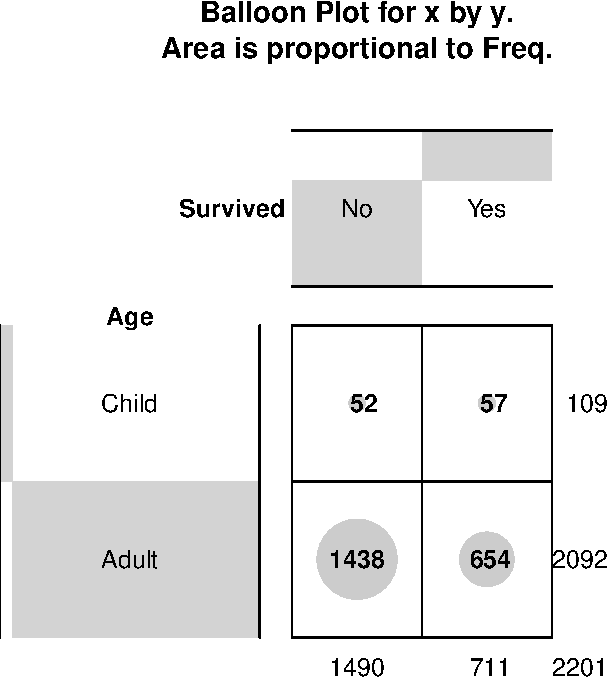
\includegraphics[width=0.4\linewidth]{NaPrzelajR_files/figure-latex/wy83-1} 

}

\caption{Przeżycie i wiek.}\label{fig:wy83}
\end{figure}

\begin{Shaded}
\begin{Highlighting}[]
\NormalTok{vcd}\OperatorTok{::}\KeywordTok{assocstats}\NormalTok{(a)}
\end{Highlighting}
\end{Shaded}

\begin{verbatim}
##                     X^2 df   P(> X^2)
## Likelihood Ratio 19.561  1 9.7458e-06
## Pearson          20.956  1 4.7008e-06
## 
## Phi-Coefficient   : 0.098 
## Contingency Coeff.: 0.097 
## Cramer's V        : 0.098
\end{verbatim}

Także i w tym przypadku istnieje zależność między zmiennymi przeżycie oraz wiek,
choć współczynnik korelacji nie jest zbyt wysoki i wynosi \(V = 0,098\).

\begin{Shaded}
\begin{Highlighting}[]
\NormalTok{pa <-}\StringTok{ }\KeywordTok{prop.table}\NormalTok{(a,}\DecValTok{2}\NormalTok{);pa}
\end{Highlighting}
\end{Shaded}

\begin{verbatim}
##         Age
## Survived     Child     Adult
##      No  0.4770642 0.6873805
##      Yes 0.5229358 0.3126195
\end{verbatim}

Po obliczeniu wartości procentowych należy stwierdzić, że katastrofę przeżyła ponad połowa dzieci \((52\%)\) oraz \(13\) osób dorosłych \((31\%)\).

\hypertarget{part_83}{%
\section{Model logitowy}\label{part_83}}

Model logitowy daje dużo większe możliwości analizy tabel wielodzielczych niż test
\(\chi^2\). Omawiane w poprzenim rozdziale testy niezależności są przeznaczone do badania
zależności dwóch zmiennych jakościowych. Natomiast za pomocą modelu logitowego
mamy możliwość analizy wielowymiarowych tabel kontyngencji. Jdnak warunek jaki
musi zostać spełniony jest taki, aby zmienna zależna była zmienną binarną. W programie R dostępna jest funkcja \href{https://rdrr.io/r/stats/glm.html}{\texttt{glm}} za pomocą której możemy estymować
parametry modelu logitowego.

\begin{Shaded}
\begin{Highlighting}[]
\CommentTok{# ustawienie punktów odniesienia: Male oraz Adult:}
\NormalTok{tt <-}\StringTok{ }\KeywordTok{transform}\NormalTok{(t,}\DataTypeTok{Sex=}\KeywordTok{relevel}\NormalTok{(Sex,}\DataTypeTok{ref=}\StringTok{"Male"}\NormalTok{),}\DataTypeTok{Age=}\KeywordTok{relevel}\NormalTok{(Age,}\DataTypeTok{ref=}\StringTok{"Adult"}\NormalTok{))}
\NormalTok{logit1 <-}\StringTok{ }\KeywordTok{glm}\NormalTok{(Survived}\OperatorTok{~}\NormalTok{.,tt,}\DataTypeTok{family=}\NormalTok{binomial)}
\KeywordTok{summary}\NormalTok{(logit1)}
\end{Highlighting}
\end{Shaded}

\begin{verbatim}
## 
## Call:
## glm(formula = Survived ~ ., family = binomial, data = tt)
## 
## Deviance Residuals: 
##     Min       1Q   Median       3Q      Max  
## -2.0812  -0.7149  -0.6656   0.6858   2.1278  
## 
## Coefficients:
##             Estimate Std. Error z value Pr(>|z|)    
## (Intercept)  -0.3762     0.1362  -2.763  0.00573 ** 
## Class2nd     -1.0181     0.1960  -5.194 2.05e-07 ***
## Class3rd     -1.7778     0.1716 -10.362  < 2e-16 ***
## ClassCrew    -0.8577     0.1573  -5.451 5.00e-08 ***
## SexFemale     2.4201     0.1404  17.236  < 2e-16 ***
## AgeChild      1.0615     0.2440   4.350 1.36e-05 ***
## ---
## Signif. codes:  0 '***' 0.001 '**' 0.01 '*' 0.05 '.' 0.1 ' ' 1
## 
## (Dispersion parameter for binomial family taken to be 1)
## 
##     Null deviance: 2769.5  on 2200  degrees of freedom
## Residual deviance: 2210.1  on 2195  degrees of freedom
## AIC: 2222.1
## 
## Number of Fisher Scoring iterations: 4
\end{verbatim}

Ten model jest dobrze dopasowany do danych. Potwierdzają to poniższe testy:

\begin{Shaded}
\begin{Highlighting}[]
\CommentTok{# test logarytmu wiarygodności:}
\NormalTok{lmtest}\OperatorTok{::}\KeywordTok{lrtest}\NormalTok{(logit1)}
\end{Highlighting}
\end{Shaded}

\begin{verbatim}
## Likelihood ratio test
## 
## Model 1: Survived ~ Class + Sex + Age
## Model 2: Survived ~ 1
##   #Df  LogLik Df Chisq Pr(>Chisq)    
## 1   6 -1105.0                        
## 2   1 -1384.7 -5 559.4  < 2.2e-16 ***
## ---
## Signif. codes:  0 '***' 0.001 '**' 0.01 '*' 0.05 '.' 0.1 ' ' 1
\end{verbatim}

\begin{Shaded}
\begin{Highlighting}[]
\CommentTok{# test reszt deviance:}
\KeywordTok{anova}\NormalTok{(logit1,}\DataTypeTok{test=}\StringTok{"Chisq"}\NormalTok{)}
\end{Highlighting}
\end{Shaded}

\begin{verbatim}
## Analysis of Deviance Table
## 
## Model: binomial, link: logit
## 
## Response: Survived
## 
## Terms added sequentially (first to last)
## 
## 
##       Df Deviance Resid. Df Resid. Dev  Pr(>Chi)    
## NULL                   2200     2769.5              
## Class  3   180.90      2197     2588.6 < 2.2e-16 ***
## Sex    1   359.64      2196     2228.9 < 2.2e-16 ***
## Age    1    18.85      2195     2210.1 1.413e-05 ***
## ---
## Signif. codes:  0 '***' 0.001 '**' 0.01 '*' 0.05 '.' 0.1 ' ' 1
\end{verbatim}

\begin{Shaded}
\begin{Highlighting}[]
\CommentTok{# adekwatność modelu:}
\DecValTok{1}\OperatorTok{-}\KeywordTok{pchisq}\NormalTok{(}\KeywordTok{deviance}\NormalTok{(logit1),logit1}\OperatorTok{$}\NormalTok{df.residual)}
\end{Highlighting}
\end{Shaded}

\begin{verbatim}
## [1] 0.4063859
\end{verbatim}

\begin{Shaded}
\begin{Highlighting}[]
\CommentTok{# dyspersja:}
\KeywordTok{sum}\NormalTok{(}\KeywordTok{resid}\NormalTok{(logit1,}\DataTypeTok{type=}\StringTok{"pearson"}\NormalTok{)}\OperatorTok{^}\DecValTok{2}\NormalTok{)}\OperatorTok{/}\KeywordTok{df.residual}\NormalTok{(logit1)}
\end{Highlighting}
\end{Shaded}

\begin{verbatim}
## [1] 1.023531
\end{verbatim}

W kolejnym kroku obliczymy ilorazy wiarygodności na podstawie oszacowanych
parametrów modelu.

\begin{Shaded}
\begin{Highlighting}[]
\KeywordTok{cbind}\NormalTok{(}\DataTypeTok{OR=}\KeywordTok{exp}\NormalTok{(}\KeywordTok{coef}\NormalTok{(logit1)))}
\end{Highlighting}
\end{Shaded}

\begin{verbatim}
##                     OR
## (Intercept)  0.6864493
## Class2nd     0.3612825
## Class3rd     0.1690159
## ClassCrew    0.4241466
## SexFemale   11.2465380
## AgeChild     2.8908263
\end{verbatim}

Interpretacja jest następująca:

\begin{itemize}
\item
  podróżowanie w drugiej klasie dało o \(64\%\) mniej szans na przeżycie niż w
  pierwszej klasie,
\item
  podróżowanie w trzeciej klasie dało o \(83\%\) mniej szans na przeżycie niż w
  pierwszej klasie,
\item
  załoga statku miała o \(58\%\) mniej szans na przeżycie niż w pierwszej klasie,
\item
  kobiety miały ponad \(11\) razy większe szanse na przeżycie od mężczyzn,
\item
  dzieci miały prawie \(2,9\) razy większe szanse na przeżycie od dorosłych.
\end{itemize}

Uogólnione modele liniowe dają także możliwość badania bardziej złożonych zależności między zmiennymi tzn. interakcji.

\begin{Shaded}
\begin{Highlighting}[]
\NormalTok{logit2=}\KeywordTok{glm}\NormalTok{(Survived}\OperatorTok{~}\NormalTok{.}\OperatorTok{^}\DecValTok{2}\NormalTok{,tt,}\DataTypeTok{family=}\NormalTok{binomial) }\CommentTok{# interakcje rzędu 2.}
\NormalTok{logit3=}\KeywordTok{glm}\NormalTok{(Survived}\OperatorTok{~}\NormalTok{.}\OperatorTok{^}\DecValTok{3}\NormalTok{,tt,}\DataTypeTok{family=}\NormalTok{binomial) }\CommentTok{# interakcje rzędu 2 i 3.}
\end{Highlighting}
\end{Shaded}

Po estymacji kilku modeli, zawsze jesteśmy zainteresowani, który z nich wybrać.
Takiego wyboru możemy dokonać np. na podstawie kryterium informacyjnego AIC.

\begin{Shaded}
\begin{Highlighting}[]
\KeywordTok{AIC}\NormalTok{(logit1,logit2,logit3)}
\end{Highlighting}
\end{Shaded}

\begin{verbatim}
##        df      AIC
## logit1  6 2222.061
## logit2 12 2121.495
## logit3 14 2125.495
\end{verbatim}

Zatem do dalszych analiz powinniśmy wybrać model \texttt{logit2} (z podwójnymi interakcjami) ponieważ charakteryzuje się najmiejszą wartością AIC. Naszą decyzję
potwierdzają także inne statystyki np. badające adekwatność modelu:

\begin{Shaded}
\begin{Highlighting}[]
\DecValTok{1}\OperatorTok{-}\KeywordTok{pchisq}\NormalTok{(}\KeywordTok{deviance}\NormalTok{(logit1),logit1}\OperatorTok{$}\NormalTok{df.residual)}
\end{Highlighting}
\end{Shaded}

\begin{verbatim}
## [1] 0.4063859
\end{verbatim}

\begin{Shaded}
\begin{Highlighting}[]
\DecValTok{1}\OperatorTok{-}\KeywordTok{pchisq}\NormalTok{(}\KeywordTok{deviance}\NormalTok{(logit2),logit2}\OperatorTok{$}\NormalTok{df.residual)}
\end{Highlighting}
\end{Shaded}

\begin{verbatim}
## [1] 0.9181299
\end{verbatim}

\begin{Shaded}
\begin{Highlighting}[]
\DecValTok{1}\OperatorTok{-}\KeywordTok{pchisq}\NormalTok{(}\KeywordTok{deviance}\NormalTok{(logit3),logit3}\OperatorTok{$}\NormalTok{df.residual)}
\end{Highlighting}
\end{Shaded}

\begin{verbatim}
## [1] 0.9134249
\end{verbatim}

oraz oceniające istotność poszczególnych interakcji:

\begin{Shaded}
\begin{Highlighting}[]
\KeywordTok{anova}\NormalTok{(logit3,}\DataTypeTok{test=}\StringTok{"Chisq"}\NormalTok{)}
\end{Highlighting}
\end{Shaded}

\begin{verbatim}
## Analysis of Deviance Table
## 
## Model: binomial, link: logit
## 
## Response: Survived
## 
## Terms added sequentially (first to last)
## 
## 
##               Df Deviance Resid. Df Resid. Dev  Pr(>Chi)    
## NULL                           2200     2769.5              
## Class          3   180.90      2197     2588.6 < 2.2e-16 ***
## Sex            1   359.64      2196     2228.9 < 2.2e-16 ***
## Age            1    18.85      2195     2210.1 1.413e-05 ***
## Class:Sex      3    66.67      2192     2143.4 2.206e-14 ***
## Class:Age      2    44.21      2190     2099.2 2.507e-10 ***
## Sex:Age        1     1.69      2189     2097.5    0.1942    
## Class:Sex:Age  2     0.00      2187     2097.5    1.0000    
## ---
## Signif. codes:  0 '***' 0.001 '**' 0.01 '*' 0.05 '.' 0.1 ' ' 1
\end{verbatim}

Tak więc najlepszym modelem okazał się \texttt{logit2}.

\begin{Shaded}
\begin{Highlighting}[]
\KeywordTok{summary}\NormalTok{(logit2)}
\end{Highlighting}
\end{Shaded}

\begin{verbatim}
## 
## Call:
## glm(formula = Survived ~ .^2, family = binomial, data = tt)
## 
## Deviance Residuals: 
##     Min       1Q   Median       3Q      Max  
## -2.6771  -0.7099  -0.5952   0.2374   2.2293  
## 
## Coefficients: (1 not defined because of singularities)
##                       Estimate Std. Error z value Pr(>|z|)    
## (Intercept)           -0.72763    0.16130  -4.511 6.45e-06 ***
## Class2nd              -1.67026    0.32240  -5.181 2.21e-07 ***
## Class3rd              -0.91330    0.20478  -4.460 8.20e-06 ***
## ClassCrew             -0.52215    0.18088  -2.887  0.00389 ** 
## SexFemale              4.28298    0.53213   8.049 8.36e-16 ***
## AgeChild              16.99213  920.38639   0.018  0.98527    
## Class2nd:SexFemale    -0.06801    0.67120  -0.101  0.91929    
## Class3rd:SexFemale    -2.79995    0.56875  -4.923 8.52e-07 ***
## ClassCrew:SexFemale   -1.13608    0.82048  -1.385  0.16616    
## Class2nd:AgeChild      0.84881 1005.81951   0.001  0.99933    
## Class3rd:AgeChild    -16.34159  920.38646  -0.018  0.98583    
## ClassCrew:AgeChild          NA         NA      NA       NA    
## SexFemale:AgeChild    -0.68679    0.52541  -1.307  0.19116    
## ---
## Signif. codes:  0 '***' 0.001 '**' 0.01 '*' 0.05 '.' 0.1 ' ' 1
## 
## (Dispersion parameter for binomial family taken to be 1)
## 
##     Null deviance: 2769.5  on 2200  degrees of freedom
## Residual deviance: 2097.5  on 2189  degrees of freedom
## AIC: 2121.5
## 
## Number of Fisher Scoring iterations: 15
\end{verbatim}

Teraz obliczymy ilorazy wiarygodności aby je zinterpretować. Wyniki zostały zaokrąglone do dwóch miejsc po przecinku za pomocą funkcji \href{https://rdrr.io/r/base/Round.html}{\texttt{round}}.

\begin{Shaded}
\begin{Highlighting}[]
\KeywordTok{cbind}\NormalTok{(}\DataTypeTok{OR=}\KeywordTok{round}\NormalTok{(}\KeywordTok{exp}\NormalTok{(}\KeywordTok{coef}\NormalTok{(logit2)),}\DecValTok{2}\NormalTok{))}
\end{Highlighting}
\end{Shaded}

\begin{verbatim}
##                              OR
## (Intercept)                0.48
## Class2nd                   0.19
## Class3rd                   0.40
## ClassCrew                  0.59
## SexFemale                 72.46
## AgeChild            23965569.64
## Class2nd:SexFemale         0.93
## Class3rd:SexFemale         0.06
## ClassCrew:SexFemale        0.32
## Class2nd:AgeChild          2.34
## Class3rd:AgeChild          0.00
## ClassCrew:AgeChild           NA
## SexFemale:AgeChild         0.50
\end{verbatim}

\begin{itemize}
\item
  szansa przeżycia osób, które podróżowały w drugiej klasie była o \(81\%\) mniejsza
  niż w pierwszej klasie,
\item
  szansa przeżycia osób, które podróżowały w trzeciej klasie była o \(60\%\) mniejsza niż w pierwszej klasie,
\item
  szansa przeżycia załogi statku była o \(41\%\) mniejsza niż w pierwszej klasie,
\item
  kobiety miały ponad \(72\) razy większe szanse na przeżycie od mężczyzn,
\item
  dzieci miały również dużo większe szanse na przeżycie od dorosłych,
\item
  szansa przeżycia kobiet, które podróżowały w trzeciej klasie była mniejsza o
  \(94\%\) niż w pierwszej klasie,
\item
  szansa przeżycia dzieci, które podróżowały w drugiej klasie była ponad \(2\) razy
  większa niż w pierwszej klasie.
\end{itemize}

Funkcja \href{https://rdrr.io/r/stats/glm.html}{\texttt{glm}} umożliwia także wybór odpowiednich zmiennych do modelu. Jeśli
np. chcielibyśmy oszacować model \texttt{logit2} ale tylko z istotnymi statystycznie parametrami to kod wyglądałby następująco:

\begin{Shaded}
\begin{Highlighting}[]
\NormalTok{myl <-}\StringTok{ }\KeywordTok{glm}\NormalTok{(Survived}\OperatorTok{~}\NormalTok{Class}\OperatorTok{+}\NormalTok{Sex}\OperatorTok{+}\NormalTok{Age}\OperatorTok{+}\KeywordTok{I}\NormalTok{(Class}\OperatorTok{==}\StringTok{"3rd"} \OperatorTok{&}\StringTok{ }\NormalTok{Sex}\OperatorTok{==}\StringTok{"Female"}\NormalTok{),tt,}
           \DataTypeTok{family=}\NormalTok{binomial)}
\KeywordTok{summary}\NormalTok{(myl)}
\end{Highlighting}
\end{Shaded}

\begin{verbatim}
## 
## Call:
## glm(formula = Survived ~ Class + Sex + Age + I(Class == "3rd" & 
##     Sex == "Female"), family = binomial, data = tt)
## 
## Deviance Residuals: 
##     Min       1Q   Median       3Q      Max  
## -2.5435  -0.7070  -0.5798   0.3842   2.0293  
## 
## Coefficients:
##                                         Estimate Std. Error z value
## (Intercept)                              -0.6337     0.1506  -4.208
## Class2nd                                 -1.2888     0.2385  -5.404
## Class3rd                                 -1.0642     0.1935  -5.500
## ClassCrew                                -0.6252     0.1708  -3.661
## SexFemale                                 3.8283     0.2715  14.098
## AgeChild                                  1.0522     0.2306   4.563
## I(Class == "3rd" & Sex == "Female")TRUE  -2.4578     0.3302  -7.443
##                                         Pr(>|z|)    
## (Intercept)                             2.57e-05 ***
## Class2nd                                6.52e-08 ***
## Class3rd                                3.80e-08 ***
## ClassCrew                               0.000252 ***
## SexFemale                                < 2e-16 ***
## AgeChild                                5.05e-06 ***
## I(Class == "3rd" & Sex == "Female")TRUE 9.81e-14 ***
## ---
## Signif. codes:  0 '***' 0.001 '**' 0.01 '*' 0.05 '.' 0.1 ' ' 1
## 
## (Dispersion parameter for binomial family taken to be 1)
## 
##     Null deviance: 2769.5  on 2200  degrees of freedom
## Residual deviance: 2145.1  on 2194  degrees of freedom
## AIC: 2159.1
## 
## Number of Fisher Scoring iterations: 5
\end{verbatim}

\hypertarget{part_84}{%
\section{Model logitowy}\label{part_84}}

Innym sposobem analizy wielowymiarowych tabel kontyngencji jest zastosowanie
modelu Poissona. Procedura estymacji i diagnostyki przebiega w taki sam sposób
jak w przypadku modelu logitowego. Należy jednak pamiętać o tym, że w tego typu
modelach zmienna zależna ma rozkład Poissona. A zatem nasz zbiór danych należy
przekształcić.

\begin{Shaded}
\begin{Highlighting}[]
\NormalTok{f <-}\StringTok{ }\KeywordTok{as.data.frame}\NormalTok{(}\KeywordTok{xtabs}\NormalTok{(}\OperatorTok{~}\NormalTok{Survived}\OperatorTok{+}\NormalTok{Class}\OperatorTok{+}\NormalTok{Sex}\OperatorTok{+}\NormalTok{Age,tt))}
\NormalTok{f[}\DecValTok{1}\OperatorTok{:}\DecValTok{3}\NormalTok{,]}
\end{Highlighting}
\end{Shaded}

\begin{verbatim}
##   Survived Class  Sex   Age Freq
## 1       No   1st Male Adult  118
## 2      Yes   1st Male Adult   57
## 3       No   2nd Male Adult  154
\end{verbatim}

\begin{Shaded}
\begin{Highlighting}[]
\NormalTok{p1 <-}\StringTok{ }\KeywordTok{glm}\NormalTok{(Freq}\OperatorTok{~}\NormalTok{.,f,}\DataTypeTok{family=}\NormalTok{poisson)}
\NormalTok{p2 <-}\StringTok{ }\KeywordTok{glm}\NormalTok{(Freq}\OperatorTok{~}\NormalTok{.}\OperatorTok{^}\DecValTok{2}\NormalTok{,f,}\DataTypeTok{family=}\NormalTok{poisson)}
\NormalTok{p3 <-}\StringTok{ }\KeywordTok{glm}\NormalTok{(Freq}\OperatorTok{~}\NormalTok{.}\OperatorTok{^}\DecValTok{3}\NormalTok{,f,}\DataTypeTok{family=}\NormalTok{poisson)}
\NormalTok{p4 <-}\StringTok{ }\KeywordTok{glm}\NormalTok{(Freq}\OperatorTok{~}\NormalTok{.}\OperatorTok{^}\DecValTok{4}\NormalTok{,f,}\DataTypeTok{family=}\NormalTok{poisson)}
\CommentTok{# kryteria informacyjne:}
\KeywordTok{AIC}\NormalTok{(p1,p2,p3,p4)}
\end{Highlighting}
\end{Shaded}

\begin{verbatim}
##    df       AIC
## p1  7 1385.0654
## p2 19  281.9902
## p3 29  185.4021
## p4 32  191.4021
\end{verbatim}

\begin{Shaded}
\begin{Highlighting}[]
\CommentTok{# adekwatność modelu:}
\DecValTok{1}\OperatorTok{-}\KeywordTok{pchisq}\NormalTok{(}\KeywordTok{deviance}\NormalTok{(p1),p1}\OperatorTok{$}\NormalTok{df.residual)}
\end{Highlighting}
\end{Shaded}

\begin{verbatim}
## [1] 0
\end{verbatim}

\begin{Shaded}
\begin{Highlighting}[]
\DecValTok{1}\OperatorTok{-}\KeywordTok{pchisq}\NormalTok{(}\KeywordTok{deviance}\NormalTok{(p2),p2}\OperatorTok{$}\NormalTok{df.residual)}
\end{Highlighting}
\end{Shaded}

\begin{verbatim}
## [1] 0
\end{verbatim}

\begin{Shaded}
\begin{Highlighting}[]
\DecValTok{1}\OperatorTok{-}\KeywordTok{pchisq}\NormalTok{(}\KeywordTok{deviance}\NormalTok{(p3),p3}\OperatorTok{$}\NormalTok{df.residual)}
\end{Highlighting}
\end{Shaded}

\begin{verbatim}
## [1] 1
\end{verbatim}

\begin{Shaded}
\begin{Highlighting}[]
\DecValTok{1}\OperatorTok{-}\KeywordTok{pchisq}\NormalTok{(}\KeywordTok{deviance}\NormalTok{(p4),p4}\OperatorTok{$}\NormalTok{df.residual)}
\end{Highlighting}
\end{Shaded}

\begin{verbatim}
## [1] 0
\end{verbatim}

\begin{Shaded}
\begin{Highlighting}[]
\CommentTok{# istotność poszczególnych interakcji:}
\KeywordTok{anova}\NormalTok{(p4,}\DataTypeTok{test=}\StringTok{"Chisq"}\NormalTok{)}
\end{Highlighting}
\end{Shaded}

\begin{verbatim}
## Analysis of Deviance Table
## 
## Model: poisson, link: log
## 
## Response: Freq
## 
## Terms added sequentially (first to last)
## 
## 
##                        Df Deviance Resid. Df Resid. Dev  Pr(>Chi)    
## NULL                                      31     4953.1              
## Survived                1   281.78        30     4671.4 < 2.2e-16 ***
## Class                   3   475.81        27     4195.5 < 2.2e-16 ***
## Sex                     1   768.32        26     3427.2 < 2.2e-16 ***
## Age                     1  2183.56        25     1243.7 < 2.2e-16 ***
## Survived:Class          3   180.90        22     1062.8 < 2.2e-16 ***
## Survived:Sex            1   434.47        21      628.3 < 2.2e-16 ***
## Survived:Age            1    19.56        20      608.7 9.746e-06 ***
## Class:Sex               3   337.77        17      271.0 < 2.2e-16 ***
## Class:Age               3   154.35        14      116.6 < 2.2e-16 ***
## Sex:Age                 1     0.02        13      116.6 0.8882240    
## Survived:Class:Sex      3    65.30        10       51.3 4.336e-14 ***
## Survived:Class:Age      3    29.34         7       22.0 1.900e-06 ***
## Survived:Sex:Age        1    12.17         6        9.8 0.0004857 ***
## Class:Sex:Age           3     9.78         3        0.0 0.0205004 *  
## Survived:Class:Sex:Age  3     0.00         0        0.0 1.0000000    
## ---
## Signif. codes:  0 '***' 0.001 '**' 0.01 '*' 0.05 '.' 0.1 ' ' 1
\end{verbatim}

\begin{Shaded}
\begin{Highlighting}[]
\CommentTok{# ilorazy wiarygodności:}
\KeywordTok{cbind}\NormalTok{(}\DataTypeTok{OR=}\KeywordTok{round}\NormalTok{(}\KeywordTok{exp}\NormalTok{(}\KeywordTok{coef}\NormalTok{(p3)),}\DecValTok{1}\NormalTok{))}
\end{Highlighting}
\end{Shaded}

\begin{verbatim}
##                                           OR
## (Intercept)                     1.180000e+02
## SurvivedYes                     5.000000e-01
## Class2nd                        1.300000e+00
## Class3rd                        3.300000e+00
## ClassCrew                       5.700000e+00
## SexFemale                       0.000000e+00
## AgeChild                        0.000000e+00
## SurvivedYes:Class2nd            2.000000e-01
## SurvivedYes:Class3rd            4.000000e-01
## SurvivedYes:ClassCrew           6.000000e-01
## SurvivedYes:SexFemale           7.250000e+01
## SurvivedYes:AgeChild            9.354350e+10
## Class2nd:SexFemale              2.500000e+00
## Class3rd:SexFemale              6.800000e+00
## ClassCrew:SexFemale             1.000000e-01
## Class2nd:AgeChild               4.000000e-01
## Class3rd:AgeChild               9.644408e+10
## ClassCrew:AgeChild              0.000000e+00
## SexFemale:AgeChild              2.000000e-01
## SurvivedYes:Class2nd:SexFemale  9.000000e-01
## SurvivedYes:Class3rd:SexFemale  1.000000e-01
## SurvivedYes:ClassCrew:SexFemale 3.000000e-01
## SurvivedYes:Class2nd:AgeChild   2.550000e+01
## SurvivedYes:Class3rd:AgeChild   0.000000e+00
## SurvivedYes:ClassCrew:AgeChild  0.000000e+00
## SurvivedYes:SexFemale:AgeChild  5.000000e-01
## Class2nd:SexFemale:AgeChild     2.500000e+00
## Class3rd:SexFemale:AgeChild     1.310000e+01
## ClassCrew:SexFemale:AgeChild    4.034000e+02
\end{verbatim}

Na podstawie otrzymanych ilorazów wiarygodności możemy również sformułować
kilka wniosków:

\begin{itemize}
\item
  szanse zgonu w poszczególnych klasach były większe niż w pierwszej klasie
  o: \(30\%\) w klasie drugiej, ponad 3 razy większe w klasie trzeciej oraz prawie
  sześciokrotnie większe wśród załogi.
\item
  szanse przeżycia w poszczególnych klasach były mniejsze niż w pierwszej klasie
  o: \(80\%\) w klasie drugiej, \(60\%\) w klasie trzeciej i \(40\%\) wśród załogi. Z kolei szansa
  przeżycia kobiet była ponad \(72\) razy większa niż mężczyzn, także dzieci miały
  wielokrotnie większe szanse na przeżycie niż dorośli.
\item
  szanse przeżycia w poszczególnych klasach wśród kobiet były mniejsze niż dla
  kobiet podróżujących w pierwszej klasie o: \(10\%\) w klasie drugiej, \(90\%\) w klasie
  trzeciej i \(70\%\) wśród żeńskiej załogi statku.
\end{itemize}

W środowisku R dostępne są także inne funkcje za pomocą których możemy ana-
lizować wielowymiarowe tabele wielodzielcze np. \href{https://rdrr.io/cran/MASS/man/loglm.html}{\texttt{MASS::loglm}} lub \href{https://rdrr.io/r/stats/loglin.html}{\texttt{loglin}}.

\hypertarget{part_9}{%
\chapter{Przykład badania rozkładu stopy zwrotu z akcji}\label{part_9}}

\begin{center}\rule{0.5\linewidth}{\linethickness}\end{center}

\hypertarget{part_9.1}{%
\section{Wprowadzenie}\label{part_9.1}}

W tym opracowaniu będziemy analizować dzienne stopy zwrotu z akcji spółki PKOBP,
która wchodzi w skład indeksu giełdowego WIG20. Indeks WIG20 to portfel akcji
dwudziestu największych i najbardziej płynnych spółek notowanych na GPW w
Warszawie. Jego skład jest ustalany po ostatniej sesji w styczniu (korekta roczna),
kwietniu, lipcu i październiku (korekty kwartalne). Akutalny stan portfela WIG20
przedstawia poniższy wykres (rys. \ref{fig:wy91}).

\begin{Shaded}
\begin{Highlighting}[]
\NormalTok{spolki1 <-}\StringTok{ }\KeywordTok{c}\NormalTok{(}\FloatTok{15.00}\NormalTok{,}\FloatTok{13.06}\NormalTok{,}\FloatTok{11.44}\NormalTok{,}\FloatTok{8.95}\NormalTok{,}\FloatTok{8.24}\NormalTok{,}\FloatTok{8.17}\NormalTok{,}\FloatTok{7.17}\NormalTok{,}\FloatTok{3.98}\NormalTok{,}\FloatTok{3.94}\NormalTok{,}\FloatTok{3.00}\NormalTok{,}\FloatTok{2.40}\NormalTok{,}
             \FloatTok{2.21}\NormalTok{,}\FloatTok{2.20}\NormalTok{,}\FloatTok{1.90}\NormalTok{,}\FloatTok{1.87}\NormalTok{,}\FloatTok{1.76}\NormalTok{,}\FloatTok{1.43}\NormalTok{,}\FloatTok{1.26}\NormalTok{,}\FloatTok{1.21}\NormalTok{,}\FloatTok{0.82}\NormalTok{)}
\NormalTok{val <-}\StringTok{ }\KeywordTok{c}\NormalTok{(}\StringTok{'15.00%'}\NormalTok{,}\StringTok{'13.06%'}\NormalTok{,}\StringTok{'11.44%'}\NormalTok{,}\StringTok{'8.95%'}\NormalTok{,}\StringTok{'8.24%'}\NormalTok{,}\StringTok{'8.17%'}\NormalTok{,}\StringTok{'7.17%'}\NormalTok{,}\StringTok{'3.98%'}\NormalTok{,}\StringTok{'3.94%'}\NormalTok{,}\StringTok{'3.00%'}\NormalTok{,}
         \StringTok{'2.40%'}\NormalTok{,}\StringTok{'2.21%'}\NormalTok{,}\StringTok{'2.20%'}\NormalTok{,}\StringTok{'1.90%'}\NormalTok{,}\StringTok{'1.87%'}\NormalTok{,}\StringTok{'1.76%'}\NormalTok{,}\StringTok{'1.43%'}\NormalTok{,}\StringTok{'1.26%'}\NormalTok{,}\StringTok{'1.21%'}\NormalTok{,}\StringTok{'0.82%'}\NormalTok{)}
\NormalTok{nam <-}\StringTok{ }\KeywordTok{c}\NormalTok{(}\StringTok{'PKOBP'}\NormalTok{,}\StringTok{'PEKAO'}\NormalTok{,}\StringTok{'KGHM'}\NormalTok{,}\StringTok{'PZU'}\NormalTok{,}\StringTok{'PGE'}\NormalTok{,}\StringTok{'PKNORLEN'}\NormalTok{,}\StringTok{'TPSA'}\NormalTok{,}\StringTok{'TAURONPE'}\NormalTok{,}\StringTok{'PGNIG'}\NormalTok{,}
         \StringTok{'BZWBK'}\NormalTok{,}\StringTok{'BRE'}\NormalTok{,}\StringTok{'ASSECOPOL'}\NormalTok{,}\StringTok{'GETIN'}\NormalTok{,}\StringTok{'GTC'}\NormalTok{,}\StringTok{'CEZ'}\NormalTok{,}\StringTok{'TVN'}\NormalTok{,}\StringTok{'PBG'}\NormalTok{,}\StringTok{'POLIMEXMS'}\NormalTok{,}
         \StringTok{'LOTOS'}\NormalTok{,}\StringTok{'CYFRPLSAT'}\NormalTok{)}
\KeywordTok{par}\NormalTok{(}\DataTypeTok{mar=}\KeywordTok{c}\NormalTok{(}\DecValTok{4}\NormalTok{,}\DecValTok{6}\NormalTok{,}\DecValTok{1}\NormalTok{,}\DecValTok{1}\NormalTok{)}\OperatorTok{+}\FloatTok{0.1}\NormalTok{, }\DataTypeTok{mgp=}\KeywordTok{c}\NormalTok{(}\DecValTok{3}\NormalTok{,}\FloatTok{0.6}\NormalTok{,}\DecValTok{0}\NormalTok{),}\DataTypeTok{las=}\DecValTok{1}\NormalTok{)}
\NormalTok{b <-}\StringTok{ }\KeywordTok{barplot}\NormalTok{(spolki1, }\DataTypeTok{names.arg=}\NormalTok{nam, }\DataTypeTok{horiz=}\OtherTok{TRUE}\NormalTok{,}\DataTypeTok{xlim=}\KeywordTok{c}\NormalTok{(}\DecValTok{0}\NormalTok{,}\DecValTok{18}\NormalTok{))}
\KeywordTok{text}\NormalTok{(spolki1, b, }\DataTypeTok{labels=}\NormalTok{val, }\DataTypeTok{pos=}\DecValTok{4}\NormalTok{)}
\end{Highlighting}
\end{Shaded}

\begin{figure}[h]

{\centering 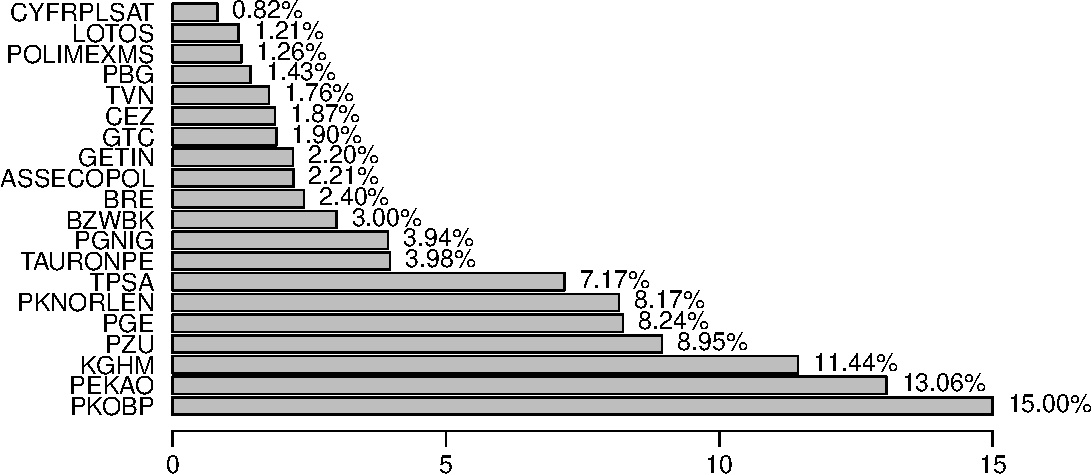
\includegraphics[width=0.7\linewidth]{NaPrzelajR_files/figure-latex/wy91-1} 

}

\caption{Struktura indeksu WIG20 -- stan na 17 grudnia 2010 r.}\label{fig:wy91}
\end{figure}

\hypertarget{part_9.2}{%
\section{Statystyki opisowe}\label{part_9.2}}

Do naszych analiz zostanie wykorzystana stopa zwrotu spółki PKOBP, która ma
największy udział w strukturze portfela WIG20 (rys. \ref{fig:wy91}). Dane dotyczące notowań na warszawskiej giełdzie papierów wartościowych są dostępne w internecie. Przykładowo, po kliknięciu w odnośnik \href{https://www.money.pl/gielda/spolki-gpw/PLPKO0000016.html}{PKOBP}
zostaniemy przekierowani do serwisu internetowego z którego można pobrać interesujące nas dane. W kolejnym kroku można samodzielnie obliczyć logarytmiczne stopy zwrotu według wzoru:
\begin{equation}
z=\ln(Close)-\ln(Open)=\ln\left(\frac{Close}{Open}\right)
\label{eq:wz91}
\end{equation}
gdzie: \(Close\) to cena zamknięcia oraz \(Open\) to cena otwarcia.

Innym rozwiązaniem jest pobranie już przetworzonego zestawu danych:

\begin{Shaded}
\begin{Highlighting}[]
\NormalTok{t <-}\StringTok{ }\KeywordTok{read.csv}\NormalTok{(}\StringTok{"https://raw.githubusercontent.com/krzysiektr/datacsv/master/pkobp.csv"}\NormalTok{)}
\KeywordTok{head}\NormalTok{(t, }\DecValTok{3}\NormalTok{)}
\end{Highlighting}
\end{Shaded}

\begin{verbatim}
##         Data Otwarcie Zamkniecie  Maks   Min Obrot_mln_zl           z
## 1 2004-11-10    14.34      15.14 15.20 14.34      2780.40 0.054287413
## 2 2004-11-12    15.14      15.26 15.94 15.14      1049.56 0.007894778
## 3 2004-11-15    15.14      15.20 15.26 14.89       425.14 0.003955180
\end{verbatim}

\begin{Shaded}
\begin{Highlighting}[]
\KeywordTok{par}\NormalTok{(}\DataTypeTok{mfcol=}\KeywordTok{c}\NormalTok{(}\DecValTok{2}\NormalTok{,}\DecValTok{1}\NormalTok{),}\DataTypeTok{mar=}\KeywordTok{c}\NormalTok{(}\DecValTok{4}\NormalTok{,}\DecValTok{4}\NormalTok{,}\DecValTok{1}\NormalTok{,}\DecValTok{1}\NormalTok{)}\OperatorTok{+}\FloatTok{0.1}\NormalTok{, }\DataTypeTok{mgp=}\KeywordTok{c}\NormalTok{(}\DecValTok{3}\NormalTok{,}\FloatTok{0.6}\NormalTok{,}\DecValTok{0}\NormalTok{),}\DataTypeTok{las=}\DecValTok{1}\NormalTok{)}
\KeywordTok{plot}\NormalTok{(}\KeywordTok{as.Date}\NormalTok{(t}\OperatorTok{$}\NormalTok{Data),t}\OperatorTok{$}\NormalTok{Zamkniecie,}\DataTypeTok{type=}\StringTok{"l"}\NormalTok{,}\DataTypeTok{main=}\StringTok{"cena zamknięcia"}\NormalTok{)}
\KeywordTok{plot}\NormalTok{(}\KeywordTok{as.Date}\NormalTok{(t}\OperatorTok{$}\NormalTok{Data),t}\OperatorTok{$}\NormalTok{z,}\DataTypeTok{type=}\StringTok{"l"}\NormalTok{,}\DataTypeTok{main=}\StringTok{"stopa zwrotu"}\NormalTok{)}
\end{Highlighting}
\end{Shaded}

\begin{figure}[h]

{\centering \includegraphics[width=0.7\linewidth]{NaPrzelajR_files/figure-latex/wy92-1} 

}

\caption{Stopy zwrotu i ceny zamknięcia od 10.11.2004 r. do 29.01.2010 r.}\label{fig:wy92}
\end{figure}

Poniżej obliczymy m.in. miary położenia tzn. średnią, medianę oraz kwartyle.

\begin{Shaded}
\begin{Highlighting}[]
\NormalTok{z <-}\StringTok{ }\NormalTok{t}\OperatorTok{$}\NormalTok{z}
\KeywordTok{summary}\NormalTok{(z)}
\end{Highlighting}
\end{Shaded}

\begin{verbatim}
##      Min.   1st Qu.    Median      Mean   3rd Qu.      Max. 
## -0.118224 -0.010002  0.001767  0.002169  0.014393  0.086565
\end{verbatim}

a także odchylenie standardowe według wzoru:
\begin{equation}
s=\sqrt{\frac{1}{n-1}\sum_{i=1}^{n}(x_i-\bar{x})^2}
\label{eq:wz92}
\end{equation}

\begin{Shaded}
\begin{Highlighting}[]
\KeywordTok{sd}\NormalTok{(z)}
\end{Highlighting}
\end{Shaded}

\begin{verbatim}
## [1] 0.02225315
\end{verbatim}

Z powyższych obliczeń wynika, że średnia stopa zwrotu w badanym okresie wyniosła
\(0,22\%\), wartość maksymalna \(8,66\%\) a minimalna \(-11,82\%\). Natomiast w wypadku \(25\%\) sesji
stopy zwrotu były mniejsze niż \(-0,01\%\), podczas \(50\%\) sesji wartości były mniejsze
niż \(0,18\%\). Z kolei w przypadku \(75\%\) sesji zysk z akcji był mniejszy niż \(1,44\%\), a w
przypadku pozostałych 25\% sesji zysk był większy niż \(1,44\%\) (rys. \ref{fig:wy93}).

Przy omawianiu różnych statystyk opisowych wato także wspomnieć o funkcji
\href{https://rdrr.io/r/stats/quantile.html}{\texttt{quantile}}. Za jej pomocą mamy możliwość obliczenia wartość dowolnego kwantyla wykorzystując jedną z dziewięciu dostępnych metod. W
tym opracowaniu zaprezentujemy sposób obliczania kwantyli za pomocą metody
siódmej. W pierwszym kroku uporządkujemy nasz wektor danych w sposób rosnący:

\begin{Shaded}
\begin{Highlighting}[]
\NormalTok{sz <-}\StringTok{ }\KeywordTok{sort}\NormalTok{(z) }\CommentTok{# wektor danych uporządkowany rosnąco}
\end{Highlighting}
\end{Shaded}

Następnie wyznaczymy numer kwantyla \(Q = 80\%\) według wzoru:
\begin{equation}
h=(n-1)\cdot Q+1
\label{eq:wz93}
\end{equation}

\begin{Shaded}
\begin{Highlighting}[]
\NormalTok{h <-}\StringTok{ }\NormalTok{(}\KeywordTok{length}\NormalTok{(z)}\OperatorTok{-}\DecValTok{1}\NormalTok{)}\OperatorTok{*}\FloatTok{0.8}\OperatorTok{+}\DecValTok{1}\NormalTok{; h }\CommentTok{# numer kwantyla}
\end{Highlighting}
\end{Shaded}

\begin{verbatim}
## [1] 1013.8
\end{verbatim}

Kolejnym krokiem będzie obliczenie wartości kwantyla na podstawie wzoru:
\begin{equation}
x_{\lfloor h \rfloor}+(h-{\lfloor h \rfloor})(x_{\lceil h\rceil}-x_{\lfloor h \rfloor})
\label{eq:wz94}
\end{equation}
gdzie: \(\lfloor h \rfloor\) to największa liczba całkowita nie większa od \texttt{h} oraz \(\lceil h \rceil\) to najmniejsza liczba całkowita nie mniejsza od \texttt{h}.

\begin{Shaded}
\begin{Highlighting}[]
\NormalTok{xL <-}\StringTok{ }\NormalTok{sz[}\KeywordTok{floor}\NormalTok{(h)]; xP <-}\StringTok{ }\NormalTok{sz[}\KeywordTok{ceiling}\NormalTok{(h)]}
\NormalTok{xL}\OperatorTok{+}\NormalTok{(h}\OperatorTok{-}\KeywordTok{floor}\NormalTok{(h))}\OperatorTok{*}\NormalTok{(xP}\OperatorTok{-}\NormalTok{xL) }\CommentTok{# wartość kwantyla}
\end{Highlighting}
\end{Shaded}

\begin{verbatim}
## [1] 0.01779921
\end{verbatim}

Teraz wykorzystamy gotową funkcję z pakietu \href{https://rdrr.io/r/\#stats}{\texttt{stats}}:

\begin{Shaded}
\begin{Highlighting}[]
\KeywordTok{quantile}\NormalTok{(z,}\FloatTok{0.80}\NormalTok{,}\DataTypeTok{type=}\DecValTok{7}\NormalTok{)}
\end{Highlighting}
\end{Shaded}

\begin{verbatim}
##        80% 
## 0.01779921
\end{verbatim}

Otrzymane wartości kwantyli możemy również zaznaczyć na wykresie (rys. \ref{fig:wy93}).

\begin{Shaded}
\begin{Highlighting}[]
\NormalTok{q <-}\StringTok{ }\KeywordTok{as.numeric}\NormalTok{(}\KeywordTok{quantile}\NormalTok{(z,}\KeywordTok{c}\NormalTok{(}\FloatTok{0.25}\NormalTok{,}\FloatTok{0.5}\NormalTok{,}\FloatTok{0.75}\NormalTok{,}\FloatTok{0.80}\NormalTok{)))}
\KeywordTok{par}\NormalTok{(}\DataTypeTok{mar=}\KeywordTok{c}\NormalTok{(}\DecValTok{4}\NormalTok{,}\DecValTok{4}\NormalTok{,}\DecValTok{1}\NormalTok{,}\DecValTok{1}\NormalTok{)}\OperatorTok{+}\FloatTok{0.1}\NormalTok{, }\DataTypeTok{mgp=}\KeywordTok{c}\NormalTok{(}\DecValTok{3}\NormalTok{,}\FloatTok{0.6}\NormalTok{,}\DecValTok{0}\NormalTok{),}\DataTypeTok{las=}\DecValTok{1}\NormalTok{)}
\KeywordTok{plot}\NormalTok{(}\KeywordTok{ecdf}\NormalTok{(z))}
\KeywordTok{arrows}\NormalTok{(q,}\KeywordTok{c}\NormalTok{(}\FloatTok{0.25}\NormalTok{,}\FloatTok{0.5}\NormalTok{,}\FloatTok{0.75}\NormalTok{,}\FloatTok{0.80}\NormalTok{),q,}\KeywordTok{c}\NormalTok{(}\DecValTok{0}\NormalTok{,}\DecValTok{0}\NormalTok{,}\DecValTok{0}\NormalTok{,}\DecValTok{0}\NormalTok{),}\DataTypeTok{length=}\FloatTok{0.1}\NormalTok{,}\DataTypeTok{angle=}\DecValTok{15}\NormalTok{,}
       \DataTypeTok{col=}\KeywordTok{c}\NormalTok{(}\StringTok{"violetred3"}\NormalTok{,}\StringTok{"YellowGreen"}\NormalTok{,}\StringTok{"SteelBlue"}\NormalTok{,}\StringTok{"wheat4"}\NormalTok{))}
\KeywordTok{arrows}\NormalTok{(q,}\KeywordTok{c}\NormalTok{(}\FloatTok{0.25}\NormalTok{,}\FloatTok{0.5}\NormalTok{,}\FloatTok{0.75}\NormalTok{,}\FloatTok{0.80}\NormalTok{),}\KeywordTok{c}\NormalTok{(}\OperatorTok{-}\DecValTok{5}\NormalTok{,}\OperatorTok{-}\DecValTok{5}\NormalTok{,}\OperatorTok{-}\DecValTok{5}\NormalTok{,}\OperatorTok{-}\DecValTok{5}\NormalTok{),}\KeywordTok{c}\NormalTok{(}\FloatTok{0.25}\NormalTok{,}\FloatTok{0.5}\NormalTok{,}\FloatTok{0.75}\NormalTok{,}\FloatTok{0.8}\NormalTok{),}\DataTypeTok{angle=}\DecValTok{0}\NormalTok{,}
       \DataTypeTok{col=}\KeywordTok{c}\NormalTok{(}\StringTok{"violetred3"}\NormalTok{,}\StringTok{"YellowGreen"}\NormalTok{,}\StringTok{"SteelBlue"}\NormalTok{,}\StringTok{"wheat4"}\NormalTok{))}
\KeywordTok{points}\NormalTok{(q,}\KeywordTok{c}\NormalTok{(}\FloatTok{0.25}\NormalTok{,}\FloatTok{0.5}\NormalTok{,}\FloatTok{0.75}\NormalTok{,}\FloatTok{0.8}\NormalTok{),}\DataTypeTok{bg=}\StringTok{"white"}\NormalTok{,}\DataTypeTok{pch=}\DecValTok{21}\NormalTok{,}
       \DataTypeTok{col=}\KeywordTok{c}\NormalTok{(}\StringTok{"violetred3"}\NormalTok{,}\StringTok{"YellowGreen"}\NormalTok{,}\StringTok{"SteelBlue"}\NormalTok{,}\StringTok{"wheat4"}\NormalTok{))}
\KeywordTok{legend}\NormalTok{(}\StringTok{"right"}\NormalTok{, }\KeywordTok{paste}\NormalTok{(}\KeywordTok{c}\NormalTok{(}\StringTok{"Q25="}\NormalTok{, }\StringTok{"Q50="}\NormalTok{, }\StringTok{"Q75="}\NormalTok{, }\StringTok{"Q80="}\NormalTok{),}\KeywordTok{round}\NormalTok{(q,}\DecValTok{4}\NormalTok{)),}\DataTypeTok{bty=}\StringTok{"n"}\NormalTok{,}\CommentTok{#lty=1,}
       \DataTypeTok{text.col=}\KeywordTok{c}\NormalTok{(}\StringTok{"violetred3"}\NormalTok{,}\StringTok{"YellowGreen"}\NormalTok{,}\StringTok{"SteelBlue"}\NormalTok{,}\StringTok{"wheat4"}\NormalTok{))}
\end{Highlighting}
\end{Shaded}

\begin{figure}[h]

{\centering \includegraphics[width=0.7\linewidth]{NaPrzelajR_files/figure-latex/wy93-1} 

}

\caption{Dystrybuanta – prezentacja graficzna kwantyli.}\label{fig:wy93}
\end{figure}

Wyznaczmy jeszcze wzory dla pozostałych metod szcowania kwantyli. Dla me-
tod od 4 do 9 algorytmy różnią się tylko sposobem wyznaczenia numeru kwantyla.
Wartość kwantyla jest obliczana tak jak to zostało przedstawione w powyższym
przykładzie czyli według wzoru \eqref{eq:wz94}

\begin{itemize}
\tightlist
\item
  typ 4:
\end{itemize}

\begin{equation}
h=n\cdot Q
\label{eq:wz95}
\end{equation}

\begin{itemize}
\tightlist
\item
  typ 5:
\end{itemize}

\begin{equation}
h=n\cdot Q + 1/2
\label{eq:wz96}
\end{equation}

\begin{itemize}
\tightlist
\item
  typ 6:
\end{itemize}

\begin{equation}
h=(n+1)\cdot Q
\label{eq:wz97}
\end{equation}

\begin{itemize}
\tightlist
\item
  typ 7:
\end{itemize}

\begin{equation}
h=(n-1)\cdot Q + 1
\label{eq:wz98}
\end{equation}

\begin{itemize}
\tightlist
\item
  typ 8:
\end{itemize}

\begin{equation}
h=(n+1/3)\cdot Q + 1/3
\label{eq:wz99}
\end{equation}

\begin{itemize}
\tightlist
\item
  typ 9:
\end{itemize}

\begin{equation}
h=(n+1/4)\cdot Q + 3/8
\label{eq:wz910}
\end{equation}

W przypadku metod od 1 do 3 do wyznaczenia numeru kwantyla oraz jego wartości
korzystamy z nastęujących wzorów:

\begin{itemize}
\tightlist
\item
  typ 1:
\end{itemize}

\begin{equation}
h=n\cdot Q +1/2 \quad\wedge\quad x_{\lceil h-1/2\rceil}
\label{eq:wz911}
\end{equation}

\begin{itemize}
\tightlist
\item
  typ 2:
\end{itemize}

\begin{equation}
h=n\cdot Q +1/2 \quad\wedge\quad (x_{\lceil h-1/2\rceil}+x_{\lfloor h+1/2\rfloor})/2
\label{eq:wz912}
\end{equation}

\begin{itemize}
\tightlist
\item
  typ 3:
\end{itemize}

\begin{equation}
h=n\cdot Q \quad\wedge\quad x_{[h]}
\label{eq:wz913}
\end{equation}

Za pomocą komendy \texttt{quantile} można także wyznaczyć jednocześnie kilka wartości
dowolnych kwantyli:

\begin{Shaded}
\begin{Highlighting}[]
\KeywordTok{quantile}\NormalTok{(z,}\KeywordTok{c}\NormalTok{(}\FloatTok{0.17}\NormalTok{,}\FloatTok{0.60}\NormalTok{,}\FloatTok{0.83}\NormalTok{),}\DataTypeTok{type=}\DecValTok{7}\NormalTok{)}
\end{Highlighting}
\end{Shaded}

\begin{verbatim}
##          17%          60%          83% 
## -0.015450594  0.006886427  0.020418864
\end{verbatim}

W różnych opracowaniach często spotykamy się z następującymi wzorami dotyczącymi skośności:
\begin{equation}
S_{1}=\frac{\frac{1}{n}\sum_{i=1}^{n}(x_i-\bar{x})^3}{\sqrt{\left(\frac{1}{n}\sum_{i=1}^{n}(x_i-\bar{x})^2\right)^3}}
\label{eq:wz914}
\end{equation}

\begin{Shaded}
\begin{Highlighting}[]
\NormalTok{(S1 <-}\StringTok{ }\NormalTok{e1071}\OperatorTok{::}\KeywordTok{skewness}\NormalTok{(z,}\DataTypeTok{type=}\DecValTok{1}\NormalTok{))}
\end{Highlighting}
\end{Shaded}

\begin{verbatim}
## [1] -0.2199644
\end{verbatim}

\begin{equation}
S_{2}=\frac{\frac{1}{n}\sum_{i=1}^{n}(x_i-\bar{x})^3\frac{\sqrt{n(n-1)}}{n-2}}{\sqrt{\left(\frac{1}{n}\sum_{i=1}^{n}(x_i-\bar{x})^2\right)^3}}
\label{eq:wz915}
\end{equation}

\begin{Shaded}
\begin{Highlighting}[]
\NormalTok{(S2 <-}\StringTok{ }\NormalTok{e1071}\OperatorTok{::}\KeywordTok{skewness}\NormalTok{(z,}\DataTypeTok{type=}\DecValTok{2}\NormalTok{))}
\end{Highlighting}
\end{Shaded}

\begin{verbatim}
## [1] -0.2202252
\end{verbatim}

\begin{equation}
S_{3}=\frac{\frac{1}{n}\sum_{i=1}^{n}(x_i-\bar{x})^3}{s^3}
\label{eq:wz916}
\end{equation}
gdzie \(\frac{1}{n}\sum_{i=1}^{n}(x_i-\bar{x})^3\) oraz \(\frac{1}{n}\sum_{i=1}^{n}(x_i-\bar{x})^2\) to odpowiednio trzeci i drugi moment
centralny oraz s to odchylenie standardowe z próby.

\begin{Shaded}
\begin{Highlighting}[]
\NormalTok{(S3 <-}\StringTok{ }\NormalTok{e1071}\OperatorTok{::}\KeywordTok{skewness}\NormalTok{(z,}\DataTypeTok{type=}\DecValTok{3}\NormalTok{))}
\end{Highlighting}
\end{Shaded}

\begin{verbatim}
## [1] -0.219704
\end{verbatim}

Ponieważ obliczony wskaźnik skośności jest równy \(-0,22\) możemy sądzić, że rozkład stopy zwrotu charakteryzuje się niewielką lewostronną skośnością.

\begin{Shaded}
\begin{Highlighting}[]
\NormalTok{moments}\OperatorTok{::}\KeywordTok{agostino.test}\NormalTok{(z)}
\end{Highlighting}
\end{Shaded}

\begin{verbatim}
## 
##  D'Agostino skewness test
## 
## data:  z
## skew = -0.21996, z = -3.17810, p-value = 0.001483
## alternative hypothesis: data have a skewness
\end{verbatim}

Również w przypadku miar koncentracji możemy spotkać się kilkoma wzorami
na kurtozę:
\begin{equation}
K_{1}=\frac{\frac{1}{n}\sum_{i=1}^{n}(x_i-\bar{x})^4}{\left(\frac{1}{n}\sum_{i=1}^{n}(x_i-\bar{x})^2\right)}-3
\label{eq:wz917}
\end{equation}

\begin{Shaded}
\begin{Highlighting}[]
\NormalTok{(K1 <-}\StringTok{ }\NormalTok{e1071}\OperatorTok{::}\KeywordTok{kurtosis}\NormalTok{(z,}\DataTypeTok{type=}\DecValTok{1}\NormalTok{))}
\end{Highlighting}
\end{Shaded}

\begin{verbatim}
## [1] 2.315957
\end{verbatim}

\begin{equation}
K_{2}=\frac{n(n+1)}{(n-1)(n-2)(n-3)}\sum_{i=1}^{n}\left(\frac{x_i-\bar{x}}{s}\right)^4-\frac{3(n-1)^2}{(n-2)(n-3)}
\label{eq:wz918}
\end{equation}

\begin{Shaded}
\begin{Highlighting}[]
\NormalTok{(K2 <-}\StringTok{ }\NormalTok{e1071}\OperatorTok{::}\KeywordTok{kurtosis}\NormalTok{(z,}\DataTypeTok{type=}\DecValTok{2}\NormalTok{))}
\end{Highlighting}
\end{Shaded}

\begin{verbatim}
## [1] 2.329873
\end{verbatim}

\begin{equation}
K_{3}=\frac{\frac{1}{n}\sum_{i=1}^{n}(x_i-\bar{x})^4}{s^4}-3
\label{eq:wz919}
\end{equation}
gdzie \(\frac{1}{n}\sum_{i=1}^{n}(x_i-\bar{x})^4\) oraz \(\frac{1}{n}\sum_{i=1}^{n}(x_i-\bar{x})^2\) to odpowiednio czwarty i drugi moment
centralny oraz \(s\) to odchylenie standardowe z próby.

\begin{Shaded}
\begin{Highlighting}[]
\NormalTok{(K3 <-}\StringTok{ }\NormalTok{e1071}\OperatorTok{::}\KeywordTok{kurtosis}\NormalTok{(z,}\DataTypeTok{type=}\DecValTok{3}\NormalTok{))}
\end{Highlighting}
\end{Shaded}

\begin{verbatim}
## [1] 2.307569
\end{verbatim}

Wysoka wartość kurtozy świadczy o tym, że rozkład stóp zwrotu charakteryzuje się
spiczastością (rozkład leptokurtyczny) w stosunku do rozkładu normalnego (rozkład
mezokurtyczny).

\begin{Shaded}
\begin{Highlighting}[]
\NormalTok{moments}\OperatorTok{::}\KeywordTok{anscombe.test}\NormalTok{(z)}
\end{Highlighting}
\end{Shaded}

\begin{verbatim}
## 
##  Anscombe-Glynn kurtosis test
## 
## data:  z
## kurt = 5.3160, z = 8.5299, p-value < 2.2e-16
## alternative hypothesis: kurtosis is not equal to 3
\end{verbatim}

\hypertarget{part_9.3}{%
\section{Rozkład normalny}\label{part_9.3}}

Funkcja gęstości rozkładu normalnego \(N(\mu,\sigma)\) dla \(\mu\in R\) oraz \(\sigma>0\) czyli \href{https://rdrr.io/r/stats/Normal.html}{\texttt{dnorm}} jest przedstawiona poniżej:
\begin{equation}
f(x)=\frac{1}{\sigma\sqrt(2\pi)}\exp\left(\frac{-(x-\mu)^2}{2\sigma^2}\right)
\label{eq:wz920}
\end{equation}
gdzie: \(\mu\) to średnia, natomiast \(\sigma\) to odchylenie standardowe.

Do estymacji nieznanych parametrów rozkładu normalnego wykorzystamy następujące funkcję:

\begin{Shaded}
\begin{Highlighting}[]
\NormalTok{a <-}\StringTok{ }\KeywordTok{mean}\NormalTok{(z); a }\CommentTok{# średnia}
\end{Highlighting}
\end{Shaded}

\begin{verbatim}
## [1] 0.00216913
\end{verbatim}

\begin{Shaded}
\begin{Highlighting}[]
\NormalTok{b <-}\StringTok{ }\KeywordTok{sd}\NormalTok{(z); b   }\CommentTok{# odchylenie standardowe}
\end{Highlighting}
\end{Shaded}

\begin{verbatim}
## [1] 0.02225315
\end{verbatim}

W przypadku gdybyśmy chcieli estymować parametry \(\mu\) oraz \(\sigma\) za pomocą funkcji \href{https://rdrr.io/r/stats/nlminb.html}{\texttt{nlminb}} kod wyglądałby następująco:

\begin{Shaded}
\begin{Highlighting}[]
\CommentTok{# logarytm funkcji wiarygodności:}
\NormalTok{f1 <-}\StringTok{ }\ControlFlowTok{function}\NormalTok{(theta, z) \{}
  \KeywordTok{sum}\NormalTok{(}\OperatorTok{-}\KeywordTok{dnorm}\NormalTok{(z, }\DataTypeTok{mean=}\NormalTok{theta[}\DecValTok{1}\NormalTok{], }\DataTypeTok{sd=}\NormalTok{theta[}\DecValTok{2}\NormalTok{], }\DataTypeTok{log=}\OtherTok{TRUE}\NormalTok{))}
\NormalTok{  \}}
\CommentTok{# parametry startowe:}
\NormalTok{p.start <-}\StringTok{ }\KeywordTok{c}\NormalTok{(}\KeywordTok{mean}\NormalTok{(z), }\KeywordTok{sd}\NormalTok{(z))}
\CommentTok{# optymalizacja funkcji f1:}
\NormalTok{e1 <-}\StringTok{ }\KeywordTok{nlminb}\NormalTok{(p.start, f1, }\DataTypeTok{z=}\NormalTok{z, }\DataTypeTok{lower=}\KeywordTok{c}\NormalTok{(}\OperatorTok{-}\OtherTok{Inf}\NormalTok{,}\DecValTok{0}\NormalTok{), }\DataTypeTok{upper=}\KeywordTok{c}\NormalTok{(}\OtherTok{Inf}\NormalTok{,}\OtherTok{Inf}\NormalTok{))}
\NormalTok{e1[}\KeywordTok{c}\NormalTok{(}\StringTok{'par'}\NormalTok{,}\StringTok{'objective'}\NormalTok{)]}
\end{Highlighting}
\end{Shaded}

\begin{verbatim}
## $par
## [1] 0.002169126 0.022244371
## 
## $objective
## [1] -3023.984
\end{verbatim}

Jak można zauważyć otrzymane parametry są dokładnie takie same jak te, które
oszacowaliśmy za pomocą funkcji \href{https://rdrr.io/r/base/mean.html}{\texttt{mean}} i \href{https://rdrr.io/r/stats/sd.html}{\texttt{sd}}.

W środowisku R można oszacować nieznane parametry również za pomocą funkcji \href{https://rdrr.io/cran/MASS/man/fitdistr.html}{\texttt{MASS::fitdistr}} lub bardziej rozbudowanej wersji \href{https://rdrr.io/cran/fitdistrplus/man/fitdist.html}{\texttt{fitdistrplus::fitdist}}. Dla wbudowanych dystrybuant nie ma konieczności podawania parametrów startowych oraz ograniczeń przedziałowych. Takie opcje są bardzo użyteczne jeśli chcemy szukać parametrów dla dystrybuant zdefiniowanych przez nas.

\begin{Shaded}
\begin{Highlighting}[]
\KeywordTok{summary}\NormalTok{(fitdistrplus}\OperatorTok{::}\KeywordTok{fitdist}\NormalTok{(z,}\StringTok{'norm'}\NormalTok{))}
\end{Highlighting}
\end{Shaded}

\begin{verbatim}
## Fitting of the distribution ' norm ' by maximum likelihood 
## Parameters : 
##        estimate   Std. Error
## mean 0.00216913 0.0006249307
## sd   0.02224437 0.0004378806
## Loglikelihood:  3023.984   AIC:  -6043.968   BIC:  -6033.679 
## Correlation matrix:
##      mean sd
## mean    1  0
## sd      0  1
\end{verbatim}

Znając już parametry \(\mu\) oraz \(\sigma\) możemy teraz przeprowadzić test zgodności
Andersona-Darlinga i odpowiedzieć na pytanie: czy stopa zwrotu PKOBP pochodzi z rozkładu normalnego?

\begin{Shaded}
\begin{Highlighting}[]
\NormalTok{ADGofTest}\OperatorTok{::}\KeywordTok{ad.test}\NormalTok{(z,pnorm,}\KeywordTok{mean}\NormalTok{(z),}\KeywordTok{sd}\NormalTok{(z))}
\end{Highlighting}
\end{Shaded}

\begin{verbatim}
## 
##  Anderson-Darling GoF Test
## 
## data:  z  and  pnorm
## AD = 7.2474, p-value = 0.0002546
## alternative hypothesis: NA
\end{verbatim}

Ponieważ \(p-value = 0.0002546\) to hipotetę zerową należy odrzucić. Zatem na
poziomie istotności \(\alpha = 0,05\) należy stwierdzić, że stopa zwrotu PKOBP nie ma rozkładu normalnego. Naszą decyzję potwierdza także (rys. \ref{fig:wy94}).

\begin{Shaded}
\begin{Highlighting}[]
\KeywordTok{par}\NormalTok{(}\DataTypeTok{mfcol=}\KeywordTok{c}\NormalTok{(}\DecValTok{1}\NormalTok{,}\DecValTok{2}\NormalTok{),}\DataTypeTok{mar=}\KeywordTok{c}\NormalTok{(}\DecValTok{4}\NormalTok{,}\DecValTok{4}\NormalTok{,}\DecValTok{1}\NormalTok{,}\DecValTok{1}\NormalTok{)}\OperatorTok{+}\FloatTok{0.1}\NormalTok{, }\DataTypeTok{mgp=}\KeywordTok{c}\NormalTok{(}\DecValTok{3}\NormalTok{,}\FloatTok{0.6}\NormalTok{,}\DecValTok{0}\NormalTok{),}\DataTypeTok{las=}\DecValTok{1}\NormalTok{)}
\KeywordTok{plot}\NormalTok{(}\KeywordTok{density}\NormalTok{(z),}\DataTypeTok{col=}\StringTok{'SteelBlue'}\NormalTok{,}\DataTypeTok{lwd=}\DecValTok{4}\NormalTok{,}\DataTypeTok{main=}\StringTok{'gęstość'}\NormalTok{)}
\KeywordTok{curve}\NormalTok{(}\KeywordTok{dnorm}\NormalTok{(x,}\KeywordTok{mean}\NormalTok{(z),}\KeywordTok{sd}\NormalTok{(z)),}\DataTypeTok{add=}\OtherTok{TRUE}\NormalTok{,}\DataTypeTok{col=}\StringTok{'violetred3'}\NormalTok{,}\DataTypeTok{lwd=}\DecValTok{3}\NormalTok{)}
\KeywordTok{legend}\NormalTok{(}\StringTok{"topright"}\NormalTok{,}\DataTypeTok{bg=}\StringTok{'white'}\NormalTok{,}\DataTypeTok{bty=}\StringTok{"n"}\NormalTok{,}\DataTypeTok{cex=}\DecValTok{1}\NormalTok{,}\DataTypeTok{lty=}\DecValTok{1}\NormalTok{,}\DataTypeTok{lwd=}\KeywordTok{c}\NormalTok{(}\DecValTok{4}\NormalTok{,}\DecValTok{3}\NormalTok{),}
       \KeywordTok{c}\NormalTok{(}\StringTok{'empiryczna'}\NormalTok{,}\StringTok{'teoretyczna'}\NormalTok{),}\DataTypeTok{col=}\KeywordTok{c}\NormalTok{(}\StringTok{'SteelBlue'}\NormalTok{,}\StringTok{'violetred3'}\NormalTok{))}
\KeywordTok{plot}\NormalTok{(}\KeywordTok{ecdf}\NormalTok{(z),}\DataTypeTok{col=}\StringTok{'SteelBlue'}\NormalTok{,}\DataTypeTok{lwd=}\DecValTok{4}\NormalTok{,}\DataTypeTok{main=}\StringTok{'dystrybuanta'}\NormalTok{)}
\KeywordTok{curve}\NormalTok{(}\KeywordTok{pnorm}\NormalTok{(x,}\KeywordTok{mean}\NormalTok{(z),}\KeywordTok{sd}\NormalTok{(z)),}\DataTypeTok{add=}\OtherTok{TRUE}\NormalTok{,}\DataTypeTok{col=}\StringTok{'violetred3'}\NormalTok{,}\DataTypeTok{lwd=}\DecValTok{3}\NormalTok{)}
\KeywordTok{legend}\NormalTok{(}\StringTok{"topleft"}\NormalTok{,}\DataTypeTok{bg=}\StringTok{'white'}\NormalTok{,}\DataTypeTok{bty=}\StringTok{"n"}\NormalTok{,}\DataTypeTok{lty=}\DecValTok{1}\NormalTok{,}\DataTypeTok{lwd=}\KeywordTok{c}\NormalTok{(}\DecValTok{4}\NormalTok{,}\DecValTok{3}\NormalTok{),}
       \KeywordTok{c}\NormalTok{(}\StringTok{'empiryczna'}\NormalTok{,}\StringTok{'teoretyczna'}\NormalTok{),}\DataTypeTok{col=}\KeywordTok{c}\NormalTok{(}\StringTok{'SteelBlue'}\NormalTok{,}\StringTok{'violetred3'}\NormalTok{))}
\end{Highlighting}
\end{Shaded}

\begin{figure}[h]

{\centering \includegraphics[width=1\linewidth]{NaPrzelajR_files/figure-latex/wy94-1} 

}

\caption{Porównanie wykresu gęstości z rozkładem normalnym.}\label{fig:wy94}
\end{figure}

\hypertarget{part_9.4}{%
\section{Rozkład Cauchy'ego}\label{part_9.4}}

Funkcja gęstości rozkładu Cauchy'ego \(C(a, b)\) dla \(a \in R\) oraz \(b > 0\) czyli \href{https://rdrr.io/r/stats/Cauchy.html}{\texttt{dcauchy}} jest przedstawiona poniżej:
\begin{equation}
f(x)=\frac{1}{\pi b \left(1+\left(\frac{x-a}{b}\right)^2\right)}
\label{eq:wz921}
\end{equation}
gdzie: \(a\) to parametr położenia, natomiast \(b\) to parametr skali.

Tak samo jak w przypadku rozkładu normalnego, aby wykorzystać funkcję \href{https://rdrr.io/r/stats/nlminb.html}{\texttt{nlminb}} należy oszacować parametry startowe. Dla rozkładu Cauchy'ego można to zrobić w
następujący sposób:

\begin{Shaded}
\begin{Highlighting}[]
\NormalTok{a <-}\StringTok{ }\KeywordTok{median}\NormalTok{(z); a }\CommentTok{# parametr położenia: a}
\end{Highlighting}
\end{Shaded}

\begin{verbatim}
## [1] 0.001766785
\end{verbatim}

\begin{Shaded}
\begin{Highlighting}[]
\NormalTok{b <-}\StringTok{ }\KeywordTok{IQR}\NormalTok{(z)}\OperatorTok{/}\DecValTok{2}\NormalTok{; b  }\CommentTok{# parametr skali: b}
\end{Highlighting}
\end{Shaded}

\begin{verbatim}
## [1] 0.0121972
\end{verbatim}

Teraz metodą największej wiarygodności oszacujemy parametry rozkładu Cauche'go.

\begin{Shaded}
\begin{Highlighting}[]
\CommentTok{# logarytm funkcji wiarygodności:}
\NormalTok{f2 <-}\StringTok{ }\ControlFlowTok{function}\NormalTok{(theta, z) \{}
  \KeywordTok{sum}\NormalTok{(}\OperatorTok{-}\KeywordTok{dcauchy}\NormalTok{(z, }\DataTypeTok{location=}\NormalTok{theta[}\DecValTok{1}\NormalTok{], }\DataTypeTok{scale=}\NormalTok{theta[}\DecValTok{2}\NormalTok{], }\DataTypeTok{log=}\OtherTok{TRUE}\NormalTok{))}
\NormalTok{  \}}
\CommentTok{# parametry startowe:}
\NormalTok{p.start <-}\StringTok{ }\KeywordTok{c}\NormalTok{(}\KeywordTok{median}\NormalTok{(z), }\KeywordTok{IQR}\NormalTok{(z)}\OperatorTok{/}\DecValTok{2}\NormalTok{)}
\CommentTok{# optymalizacja funkcji f2:}
\NormalTok{e2 <-}\StringTok{ }\KeywordTok{nlminb}\NormalTok{(p.start, f2, }\DataTypeTok{z=}\NormalTok{z, }\DataTypeTok{lower=}\KeywordTok{c}\NormalTok{(}\OperatorTok{-}\OtherTok{Inf}\NormalTok{,}\DecValTok{0}\NormalTok{), }\DataTypeTok{upper=}\KeywordTok{c}\NormalTok{(}\OtherTok{Inf}\NormalTok{,}\OtherTok{Inf}\NormalTok{))}
\NormalTok{e2[}\KeywordTok{c}\NormalTok{(}\StringTok{'par'}\NormalTok{,}\StringTok{'objective'}\NormalTok{)]}
\end{Highlighting}
\end{Shaded}

\begin{verbatim}
## $par
## [1] 0.002025263 0.011231456
## 
## $objective
## [1] -2945.315
\end{verbatim}

Prawie identyczne wyniki otrzymamy przy wykorzystaniu funkcji \href{https://rdrr.io/cran/fitdistrplus/man/fitdist.html}{\texttt{fitdistrplus::fitdist}}.

\begin{Shaded}
\begin{Highlighting}[]
\KeywordTok{summary}\NormalTok{(fitdistrplus}\OperatorTok{::}\KeywordTok{fitdist}\NormalTok{(z,}\StringTok{'cauchy'}\NormalTok{))}
\end{Highlighting}
\end{Shaded}

\begin{verbatim}
## Fitting of the distribution ' cauchy ' by maximum likelihood 
## Parameters : 
##             estimate   Std. Error
## location 0.002029574 0.0004912212
## scale    0.011230842 0.0004071368
## Loglikelihood:  2945.315   AIC:  -5886.63   BIC:  -5876.341 
## Correlation matrix:
##            location      scale
## location 1.00000000 0.03089075
## scale    0.03089075 1.00000000
\end{verbatim}

Do sprawdzenia zgoności rozkładu empirycznego z rozkładem Cauchy'ego zastosujemy test Andersona-Darlinga.

\begin{Shaded}
\begin{Highlighting}[]
\NormalTok{ADGofTest}\OperatorTok{::}\KeywordTok{ad.test}\NormalTok{(z,pcauchy, }\FloatTok{0.002029574}\NormalTok{, }\FloatTok{0.011230842}\NormalTok{)}
\end{Highlighting}
\end{Shaded}

\begin{verbatim}
## 
##  Anderson-Darling GoF Test
## 
## data:  z  and  pcauchy
## AD = 10.36, p-value = 3.782e-06
## alternative hypothesis: NA
\end{verbatim}

Także i w tym razem na poziomie istotności \(\alpha = 0,05\) odrzucamy hipotezę zerową, która zakłada, że stopa zwrotu ma rozkład Cauchy'ego.

\begin{Shaded}
\begin{Highlighting}[]
\KeywordTok{par}\NormalTok{(}\DataTypeTok{mfcol=}\KeywordTok{c}\NormalTok{(}\DecValTok{1}\NormalTok{,}\DecValTok{2}\NormalTok{),}\DataTypeTok{mar=}\KeywordTok{c}\NormalTok{(}\DecValTok{4}\NormalTok{,}\DecValTok{4}\NormalTok{,}\DecValTok{1}\NormalTok{,}\DecValTok{1}\NormalTok{)}\OperatorTok{+}\FloatTok{0.1}\NormalTok{, }\DataTypeTok{mgp=}\KeywordTok{c}\NormalTok{(}\DecValTok{3}\NormalTok{,}\FloatTok{0.6}\NormalTok{,}\DecValTok{0}\NormalTok{),}\DataTypeTok{las=}\DecValTok{1}\NormalTok{)}
\KeywordTok{plot}\NormalTok{(}\KeywordTok{density}\NormalTok{(z),}\DataTypeTok{col=}\StringTok{'SteelBlue'}\NormalTok{,}\DataTypeTok{lwd=}\DecValTok{4}\NormalTok{,}\DataTypeTok{main=}\StringTok{'gęstość'}\NormalTok{,}\DataTypeTok{ylim=}\KeywordTok{c}\NormalTok{(}\DecValTok{0}\NormalTok{,}\DecValTok{30}\NormalTok{))}
\KeywordTok{curve}\NormalTok{(}\KeywordTok{dcauchy}\NormalTok{(x,}\FloatTok{0.002029574}\NormalTok{, }\FloatTok{0.011230842}\NormalTok{),}\DataTypeTok{add=}\OtherTok{TRUE}\NormalTok{,}\DataTypeTok{col=}\StringTok{'violetred3'}\NormalTok{,}\DataTypeTok{lwd=}\DecValTok{3}\NormalTok{)}
\KeywordTok{legend}\NormalTok{(}\StringTok{"topright"}\NormalTok{,}\DataTypeTok{bg=}\StringTok{'white'}\NormalTok{,}\DataTypeTok{bty=}\StringTok{"n"}\NormalTok{,}\DataTypeTok{cex=}\DecValTok{1}\NormalTok{,}\DataTypeTok{lty=}\DecValTok{1}\NormalTok{,}\DataTypeTok{lwd=}\KeywordTok{c}\NormalTok{(}\DecValTok{4}\NormalTok{,}\DecValTok{3}\NormalTok{),}
       \KeywordTok{c}\NormalTok{(}\StringTok{'empiryczna'}\NormalTok{,}\StringTok{'teoretyczna'}\NormalTok{),}\DataTypeTok{col=}\KeywordTok{c}\NormalTok{(}\StringTok{'SteelBlue'}\NormalTok{,}\StringTok{'violetred3'}\NormalTok{))}
\KeywordTok{plot}\NormalTok{(}\KeywordTok{ecdf}\NormalTok{(z),}\DataTypeTok{col=}\StringTok{'SteelBlue'}\NormalTok{,}\DataTypeTok{lwd=}\DecValTok{4}\NormalTok{,}\DataTypeTok{main=}\StringTok{'dystrybuanta'}\NormalTok{)}
\KeywordTok{curve}\NormalTok{(}\KeywordTok{pcauchy}\NormalTok{(x,}\FloatTok{0.002029574}\NormalTok{, }\FloatTok{0.011230842}\NormalTok{),}\DataTypeTok{add=}\OtherTok{TRUE}\NormalTok{,}\DataTypeTok{col=}\StringTok{'violetred3'}\NormalTok{,}\DataTypeTok{lwd=}\DecValTok{3}\NormalTok{)}
\KeywordTok{legend}\NormalTok{(}\StringTok{"topleft"}\NormalTok{,}\DataTypeTok{bg=}\StringTok{'white'}\NormalTok{,}\DataTypeTok{bty=}\StringTok{"n"}\NormalTok{,}\DataTypeTok{lty=}\DecValTok{1}\NormalTok{,}\DataTypeTok{lwd=}\KeywordTok{c}\NormalTok{(}\DecValTok{4}\NormalTok{,}\DecValTok{3}\NormalTok{),}
       \KeywordTok{c}\NormalTok{(}\StringTok{'empiryczna'}\NormalTok{,}\StringTok{'teoretyczna'}\NormalTok{),}\DataTypeTok{col=}\KeywordTok{c}\NormalTok{(}\StringTok{'SteelBlue'}\NormalTok{,}\StringTok{'violetred3'}\NormalTok{))}
\end{Highlighting}
\end{Shaded}

\begin{figure}[h]

{\centering \includegraphics[width=1\linewidth]{NaPrzelajR_files/figure-latex/wy95-1} 

}

\caption{Porównanie wykresu gęstości z rozkładem Cauchy`ego.}\label{fig:wy95}
\end{figure}

\hypertarget{part_9.5}{%
\section{Rozkład Laplace'a}\label{part_9.5}}

Funkcja gęstości rozkładu Laplace'a \(L(a, b)\) dla \(a \in R\) oraz \(b > 0\) czyli \href{https://rdrr.io/cran/VGAM/man/laplaceUC.html}{\texttt{VGAM::dlaplace}} jest przedstawiona poniżej:
\begin{equation}
f(x)=\frac{1}{2b}\exp\left(\frac{-|x-a|}{b}\right)
\label{eq:wz922}
\end{equation}
gdzie: \(a\) to parametr położenia, natomiast \(b\) to parametr skali.

Parametry startowe oszacujemy w następujący sposób:

\begin{Shaded}
\begin{Highlighting}[]
\NormalTok{a <-}\StringTok{ }\KeywordTok{median}\NormalTok{(z); a     }\CommentTok{# parametr położenia: a}
\end{Highlighting}
\end{Shaded}

\begin{verbatim}
## [1] 0.001766785
\end{verbatim}

\begin{Shaded}
\begin{Highlighting}[]
\NormalTok{b <-}\StringTok{ }\KeywordTok{mean}\NormalTok{(}\KeywordTok{abs}\NormalTok{(z}\OperatorTok{-}\KeywordTok{median}\NormalTok{(z))); b }\CommentTok{# parametr skali: b}
\end{Highlighting}
\end{Shaded}

\begin{verbatim}
## [1] 0.01628686
\end{verbatim}

Mając do dyspozycji funkcję gęstości \href{https://rdrr.io/cran/VGAM/man/laplaceUC.html}{\texttt{VGAM::dlaplace}} oraz parametry startowe dokonamy estymacji parametrów \texttt{a} oraz \texttt{b} dla rozkładu Laplace'a.

\begin{Shaded}
\begin{Highlighting}[]
\CommentTok{# logarytm funkcji wiarygodności:}
\NormalTok{f3 <-}\StringTok{ }\ControlFlowTok{function}\NormalTok{(theta, z) \{}
  \KeywordTok{sum}\NormalTok{(}\OperatorTok{-}\NormalTok{VGAM}\OperatorTok{::}\KeywordTok{dlaplace}\NormalTok{(z, }\DataTypeTok{location=}\NormalTok{theta[}\DecValTok{1}\NormalTok{], }\DataTypeTok{scale=}\NormalTok{theta[}\DecValTok{2}\NormalTok{], }\DataTypeTok{log=}\OtherTok{TRUE}\NormalTok{))}
\NormalTok{  \}}
\CommentTok{# parametry startowe:}
\NormalTok{p.start <-}\StringTok{ }\KeywordTok{c}\NormalTok{(}\KeywordTok{median}\NormalTok{(z), }\KeywordTok{mean}\NormalTok{(}\KeywordTok{abs}\NormalTok{(z}\OperatorTok{-}\KeywordTok{median}\NormalTok{(z))))}
\CommentTok{# optymalizacja funkcji f3:}
\NormalTok{e3 <-}\StringTok{ }\KeywordTok{nlminb}\NormalTok{(p.start, f3, }\DataTypeTok{z=}\NormalTok{z, }\DataTypeTok{lower=}\KeywordTok{c}\NormalTok{(}\OperatorTok{-}\OtherTok{Inf}\NormalTok{,}\DecValTok{0}\NormalTok{), }\DataTypeTok{upper=}\KeywordTok{c}\NormalTok{(}\OtherTok{Inf}\NormalTok{,}\OtherTok{Inf}\NormalTok{))}
\NormalTok{e3}
\end{Highlighting}
\end{Shaded}

\begin{verbatim}
## $par
## [1] 0.001766785 0.016286861
## 
## $objective
## [1] -3071.524
## 
## $convergence
## [1] 1
## 
## $iterations
## [1] 1
## 
## $evaluations
## function gradient 
##       25        2 
## 
## $message
## [1] "false convergence (8)"
\end{verbatim}

Stosowanie algorytmów optymalizacyjnych ogólnego przeznaczenia np. \href{https://rdrr.io/r/stats/nlminb.html}{\texttt{nlminb}} do wyznaczania parametrów funkcji
wymaga podawania parametrów startowych. Jeśli nie chcemy ich podawać
warto skorzystać z funkcj \href{https://rdrr.io/cran/VGAM/man/vglm.html}{\texttt{VGAM::vglm}}.
Za jej pomocą można oszacować szukane parametry dla wielu ciekawych rozkładów np. Laplace'a.

\begin{Shaded}
\begin{Highlighting}[]
\NormalTok{fit <-}\StringTok{ }\NormalTok{VGAM}\OperatorTok{::}\KeywordTok{vglm}\NormalTok{(z }\OperatorTok{~}\StringTok{ }\DecValTok{1}\NormalTok{, VGAM}\OperatorTok{::}\NormalTok{laplace, }\KeywordTok{data.frame}\NormalTok{(z), }\DataTypeTok{trace=}\OtherTok{FALSE}\NormalTok{, }\DataTypeTok{crit=}\StringTok{"l"}\NormalTok{)}
\NormalTok{VGAM}\OperatorTok{::}\KeywordTok{Coef}\NormalTok{(fit)}
\end{Highlighting}
\end{Shaded}

\begin{verbatim}
##    location       scale 
## 0.001766785 0.016296640
\end{verbatim}

\begin{Shaded}
\begin{Highlighting}[]
\NormalTok{ADGofTest}\OperatorTok{::}\KeywordTok{ad.test}\NormalTok{(z,VGAM}\OperatorTok{::}\NormalTok{plaplace, }\FloatTok{0.001766785}\NormalTok{, }\FloatTok{0.016296640}\NormalTok{)}
\end{Highlighting}
\end{Shaded}

\begin{verbatim}
## 
##  Anderson-Darling GoF Test
## 
## data:  z  and  VGAM::plaplace
## AD = 1.4474, p-value = 0.1896
## alternative hypothesis: NA
\end{verbatim}

Ponieważ \(p-value = 0.1896\), więc nie ma podstaw do odrzucenia hipotezy zerowej.
Zatem można przyjąć, że rozkład stóp zwrotu spółki PKOBP ma rozkład Laplace'a.

\begin{Shaded}
\begin{Highlighting}[]
\KeywordTok{par}\NormalTok{(}\DataTypeTok{mfcol=}\KeywordTok{c}\NormalTok{(}\DecValTok{1}\NormalTok{,}\DecValTok{2}\NormalTok{),}\DataTypeTok{mar=}\KeywordTok{c}\NormalTok{(}\DecValTok{4}\NormalTok{,}\DecValTok{4}\NormalTok{,}\DecValTok{1}\NormalTok{,}\DecValTok{1}\NormalTok{)}\OperatorTok{+}\FloatTok{0.1}\NormalTok{, }\DataTypeTok{mgp=}\KeywordTok{c}\NormalTok{(}\DecValTok{3}\NormalTok{,}\FloatTok{0.6}\NormalTok{,}\DecValTok{0}\NormalTok{),}\DataTypeTok{las=}\DecValTok{1}\NormalTok{)}
\KeywordTok{plot}\NormalTok{(}\KeywordTok{density}\NormalTok{(z),}\DataTypeTok{col=}\StringTok{'SteelBlue'}\NormalTok{,}\DataTypeTok{lwd=}\DecValTok{4}\NormalTok{,}\DataTypeTok{main=}\StringTok{'gęstość'}\NormalTok{,}\DataTypeTok{ylim=}\KeywordTok{c}\NormalTok{(}\DecValTok{0}\NormalTok{,}\DecValTok{30}\NormalTok{))}
\KeywordTok{curve}\NormalTok{(VGAM}\OperatorTok{::}\KeywordTok{dlaplace}\NormalTok{(x,}\FloatTok{0.001766785}\NormalTok{, }\FloatTok{0.016296640}\NormalTok{),}\DataTypeTok{add=}\OtherTok{TRUE}\NormalTok{,}\DataTypeTok{col=}\StringTok{'violetred3'}\NormalTok{,}\DataTypeTok{lwd=}\DecValTok{3}\NormalTok{)}
\KeywordTok{legend}\NormalTok{(}\StringTok{"topright"}\NormalTok{,}\DataTypeTok{bg=}\StringTok{'white'}\NormalTok{,}\DataTypeTok{bty=}\StringTok{"n"}\NormalTok{,}\DataTypeTok{cex=}\DecValTok{1}\NormalTok{,}\DataTypeTok{lty=}\DecValTok{1}\NormalTok{,}\DataTypeTok{lwd=}\KeywordTok{c}\NormalTok{(}\DecValTok{4}\NormalTok{,}\DecValTok{3}\NormalTok{),}
       \KeywordTok{c}\NormalTok{(}\StringTok{'empiryczna'}\NormalTok{,}\StringTok{'teoretyczna'}\NormalTok{),}\DataTypeTok{col=}\KeywordTok{c}\NormalTok{(}\StringTok{'SteelBlue'}\NormalTok{,}\StringTok{'violetred3'}\NormalTok{))}
\KeywordTok{plot}\NormalTok{(}\KeywordTok{ecdf}\NormalTok{(z),}\DataTypeTok{col=}\StringTok{'SteelBlue'}\NormalTok{,}\DataTypeTok{lwd=}\DecValTok{4}\NormalTok{,}\DataTypeTok{main=}\StringTok{'dystrybuanta'}\NormalTok{)}
\KeywordTok{curve}\NormalTok{(VGAM}\OperatorTok{::}\KeywordTok{plaplace}\NormalTok{(x,}\FloatTok{0.001766785}\NormalTok{, }\FloatTok{0.016296640}\NormalTok{),}\DataTypeTok{add=}\OtherTok{TRUE}\NormalTok{,}\DataTypeTok{col=}\StringTok{'violetred3'}\NormalTok{,}\DataTypeTok{lwd=}\DecValTok{3}\NormalTok{)}
\KeywordTok{legend}\NormalTok{(}\StringTok{"topleft"}\NormalTok{,}\DataTypeTok{bg=}\StringTok{'white'}\NormalTok{,}\DataTypeTok{bty=}\StringTok{"n"}\NormalTok{,}\DataTypeTok{lty=}\DecValTok{1}\NormalTok{,}\DataTypeTok{lwd=}\KeywordTok{c}\NormalTok{(}\DecValTok{4}\NormalTok{,}\DecValTok{3}\NormalTok{),}
       \KeywordTok{c}\NormalTok{(}\StringTok{'empiryczna'}\NormalTok{,}\StringTok{'teoretyczna'}\NormalTok{),}\DataTypeTok{col=}\KeywordTok{c}\NormalTok{(}\StringTok{'SteelBlue'}\NormalTok{,}\StringTok{'violetred3'}\NormalTok{))}
\end{Highlighting}
\end{Shaded}

\begin{figure}[h]

{\centering \includegraphics[width=1\linewidth]{NaPrzelajR_files/figure-latex/wy96-1} 

}

\caption{Porównanie wykresu gęstości z rozkładem Laplace`a.}\label{fig:wy96}
\end{figure}

\hypertarget{part_9.6}{%
\section{Rozkład Stabilny}\label{part_9.6}}

Rozkład stabilny \(S(\alpha, \beta, \gamma, \delta)\), gdzie \(\alpha \in(0; 2)\) to parametr kształtu, \(\beta \in(-1; 1)\)
to indeks skośności, \(\gamma > 0\) to parametr skali, oraz \(\delta \in R\) to parametr położenia,
nie ma ściśle określonej funkcji gęstości -- \href{https://rdrr.io/cran/stabledist/man/dist-stable.html}{\texttt{stabledist::dstable}}. W zależności od wartości parametrów \(\alpha\)
oraz \(\beta\) możemy otrzymać rozkłady, takie jak: rozkład normalny: \(\alpha = 2\), rozkład
Cauchy'ego: \(\alpha = 1\) i \(\beta = 0\) oraz rozkład Levy'ego: \(\alpha = 12\) i \(\beta = -1\).

Do oszacowania parametrów rozkładu stabilnego można wykorzystać funkcję \href{https://rdrr.io/cran/libstableR/man/stable_fit.html}{\texttt{libstableR::stable\_fit\_mle}} która stosuje metodę największej wiarygodności.

\begin{Shaded}
\begin{Highlighting}[]
\NormalTok{p <-}\StringTok{ }\NormalTok{libstableR}\OperatorTok{::}\KeywordTok{stable_fit_mle}\NormalTok{(z)}
\end{Highlighting}
\end{Shaded}

\begin{verbatim}
## INIT MCCULLCOH
\end{verbatim}

\begin{Shaded}
\begin{Highlighting}[]
\NormalTok{p}
\end{Highlighting}
\end{Shaded}

\begin{verbatim}
## [1]  1.7281736156 -0.0007958884  0.0132426670  0.0023446287
\end{verbatim}

\begin{Shaded}
\begin{Highlighting}[]
\NormalTok{ADGofTest}\OperatorTok{::}\KeywordTok{ad.test}\NormalTok{(z,stabledist}\OperatorTok{::}\NormalTok{pstable,p[}\DecValTok{1}\NormalTok{],p[}\DecValTok{2}\NormalTok{],p[}\DecValTok{3}\NormalTok{],p[}\DecValTok{4}\NormalTok{])}
\end{Highlighting}
\end{Shaded}

\begin{verbatim}
## 
##  Anderson-Darling GoF Test
## 
## data:  z  and  stabledist::pstable
## AD = 0.72666, p-value = 0.5369
## alternative hypothesis: NA
\end{verbatim}

Test Andersona-Darlinga wykazał, że badana zmienna ma rozkład stabilny o parametrach: \(\alpha = 1,73\), \(\beta = -0,000796\), \(\gamma = 0,01\) oraz \(\delta = 0,002\). Warto zwrócić
uwagę na wysokość p-value dla rozkładu stabilnego, które wynosi \(0,5369\) i jest większa
niż dla rozkładu Laplace'a \((0,1896)\). A zatem należy sądzić, że właśnie ten rozkład
lepiej opisuje badaną zmienną (rys. \ref{fig:wy97}).

\begin{Shaded}
\begin{Highlighting}[]
\KeywordTok{par}\NormalTok{(}\DataTypeTok{mfcol=}\KeywordTok{c}\NormalTok{(}\DecValTok{1}\NormalTok{,}\DecValTok{2}\NormalTok{),}\DataTypeTok{mar=}\KeywordTok{c}\NormalTok{(}\DecValTok{4}\NormalTok{,}\DecValTok{4}\NormalTok{,}\DecValTok{1}\NormalTok{,}\DecValTok{1}\NormalTok{)}\OperatorTok{+}\FloatTok{0.1}\NormalTok{, }\DataTypeTok{mgp=}\KeywordTok{c}\NormalTok{(}\DecValTok{3}\NormalTok{,}\FloatTok{0.6}\NormalTok{,}\DecValTok{0}\NormalTok{),}\DataTypeTok{las=}\DecValTok{1}\NormalTok{)}
\KeywordTok{plot}\NormalTok{(}\KeywordTok{density}\NormalTok{(z),}\DataTypeTok{col=}\StringTok{'SteelBlue'}\NormalTok{,}\DataTypeTok{lwd=}\DecValTok{4}\NormalTok{,}\DataTypeTok{main=}\StringTok{'gęstość'}\NormalTok{)}
\KeywordTok{curve}\NormalTok{(stabledist}\OperatorTok{::}\KeywordTok{dstable}\NormalTok{(x, }\FloatTok{1.7281736156}\NormalTok{, }\FloatTok{-0.0007958884}\NormalTok{, }\FloatTok{0.0132426670}\NormalTok{,  }\FloatTok{0.0023446287}\NormalTok{),}
      \DataTypeTok{add=}\OtherTok{TRUE}\NormalTok{,}\DataTypeTok{col=}\StringTok{'violetred3'}\NormalTok{,}\DataTypeTok{lwd=}\DecValTok{3}\NormalTok{)}
\KeywordTok{legend}\NormalTok{(}\StringTok{"topright"}\NormalTok{,}\DataTypeTok{bg=}\StringTok{'white'}\NormalTok{,}\DataTypeTok{bty=}\StringTok{"n"}\NormalTok{,}\DataTypeTok{cex=}\DecValTok{1}\NormalTok{,}\DataTypeTok{lty=}\DecValTok{1}\NormalTok{,}\DataTypeTok{lwd=}\KeywordTok{c}\NormalTok{(}\DecValTok{4}\NormalTok{,}\DecValTok{3}\NormalTok{),}
\KeywordTok{c}\NormalTok{(}\StringTok{'empiryczna'}\NormalTok{,}\StringTok{'teoretyczna'}\NormalTok{),}\DataTypeTok{col=}\KeywordTok{c}\NormalTok{(}\StringTok{'SteelBlue'}\NormalTok{,}\StringTok{'violetred3'}\NormalTok{))}
\KeywordTok{plot}\NormalTok{(}\KeywordTok{ecdf}\NormalTok{(z),}\DataTypeTok{col=}\StringTok{'SteelBlue'}\NormalTok{,}\DataTypeTok{lwd=}\DecValTok{4}\NormalTok{,}\DataTypeTok{main=}\StringTok{'dystrybuanta'}\NormalTok{)}
\KeywordTok{curve}\NormalTok{(stabledist}\OperatorTok{::}\KeywordTok{pstable}\NormalTok{(x, }\FloatTok{1.7281736156}\NormalTok{, }\FloatTok{-0.0007958884}\NormalTok{, }\FloatTok{0.0132426670}\NormalTok{,  }\FloatTok{0.0023446287}\NormalTok{),}
      \DataTypeTok{add=}\OtherTok{TRUE}\NormalTok{,}\DataTypeTok{col=}\StringTok{'violetred3'}\NormalTok{,}\DataTypeTok{lwd=}\DecValTok{3}\NormalTok{)}
\KeywordTok{legend}\NormalTok{(}\StringTok{"topleft"}\NormalTok{,}\DataTypeTok{bg=}\StringTok{'white'}\NormalTok{,}\DataTypeTok{bty=}\StringTok{"n"}\NormalTok{,}\DataTypeTok{lty=}\DecValTok{1}\NormalTok{,}\DataTypeTok{lwd=}\KeywordTok{c}\NormalTok{(}\DecValTok{4}\NormalTok{,}\DecValTok{3}\NormalTok{),}
\KeywordTok{c}\NormalTok{(}\StringTok{'empiryczna'}\NormalTok{,}\StringTok{'teoretyczna'}\NormalTok{),}\DataTypeTok{col=}\KeywordTok{c}\NormalTok{(}\StringTok{'SteelBlue'}\NormalTok{,}\StringTok{'violetred3'}\NormalTok{))}
\end{Highlighting}
\end{Shaded}

\begin{figure}[h]

{\centering \includegraphics[width=1\linewidth]{NaPrzelajR_files/figure-latex/wy97-1} 

}

\caption{Porównanie wykresu gęstości z rozkładem Stabilnym.}\label{fig:wy97}
\end{figure}

Znając rozkład badanej zmiennej można także obliczyć prawdopodobieństwo wystąpienia określonej stopy zwrotu. W tym celu wykorzystamy funkcję \href{https://rdrr.io/cran/stabledist/man/dist-stable.html}{\texttt{stabledist::pstable}}
czyli dystrybuantę rozkładu stabilnego.

\begin{enumerate}
\def\labelenumi{\arabic{enumi}.}
\tightlist
\item
  Jakie jest prawdopodobieństwo, że stopa zwrotu będzie mniejsza niż \(2\%\)?
  \[P(z<0,02)\]
\end{enumerate}

\begin{Shaded}
\begin{Highlighting}[]
\NormalTok{a <-}\StringTok{ }\NormalTok{p[}\DecValTok{1}\NormalTok{]}
\NormalTok{b <-}\StringTok{ }\NormalTok{p[}\DecValTok{2}\NormalTok{]}
\NormalTok{g <-}\StringTok{ }\NormalTok{p[}\DecValTok{3}\NormalTok{]}
\NormalTok{d <-}\StringTok{ }\NormalTok{p[}\DecValTok{4}\NormalTok{]}
\NormalTok{stabledist}\OperatorTok{::}\KeywordTok{pstable}\NormalTok{(}\FloatTok{0.02}\NormalTok{, a,b,g,d)}
\end{Highlighting}
\end{Shaded}

\begin{verbatim}
## [1] 0.821845
\end{verbatim}

\begin{Shaded}
\begin{Highlighting}[]
\KeywordTok{par}\NormalTok{(}\DataTypeTok{mar=}\KeywordTok{c}\NormalTok{(}\DecValTok{4}\NormalTok{,}\DecValTok{4}\NormalTok{,}\DecValTok{1}\NormalTok{,}\DecValTok{1}\NormalTok{)}\OperatorTok{+}\FloatTok{0.1}\NormalTok{, }\DataTypeTok{mgp=}\KeywordTok{c}\NormalTok{(}\DecValTok{3}\NormalTok{,}\FloatTok{0.6}\NormalTok{,}\DecValTok{0}\NormalTok{),}\DataTypeTok{las=}\DecValTok{1}\NormalTok{)}
\KeywordTok{curve}\NormalTok{(stabledist}\OperatorTok{::}\KeywordTok{dstable}\NormalTok{(x,a,b,g,d),}\OperatorTok{-}\FloatTok{0.1}\NormalTok{,}\FloatTok{0.1}\NormalTok{,}
      \DataTypeTok{col=}\StringTok{'white'}\NormalTok{, }\DataTypeTok{main=}\StringTok{'prawdopodobieństwo'}\NormalTok{)}
\NormalTok{x <-}\StringTok{ }\KeywordTok{seq}\NormalTok{(}\FloatTok{0.02}\NormalTok{,}\OperatorTok{-}\FloatTok{0.1}\NormalTok{,}\DataTypeTok{length=}\DecValTok{300}\NormalTok{)}
\NormalTok{y <-}\StringTok{ }\NormalTok{stabledist}\OperatorTok{::}\KeywordTok{dstable}\NormalTok{(x,a,b,g,d)}
\KeywordTok{polygon}\NormalTok{(}\KeywordTok{c}\NormalTok{(}\FloatTok{0.02}\NormalTok{,x,}\OperatorTok{-}\FloatTok{0.1}\NormalTok{),}\KeywordTok{c}\NormalTok{(}\DecValTok{0}\NormalTok{,y,}\DecValTok{0}\NormalTok{),}
        \DataTypeTok{col=}\StringTok{'Violet'}\NormalTok{,}\DataTypeTok{border =} \StringTok{"Dark Magenta"}\NormalTok{)}
\KeywordTok{curve}\NormalTok{(stabledist}\OperatorTok{::}\KeywordTok{dstable}\NormalTok{(x,a,b,g,d),}\OperatorTok{-}\FloatTok{0.1}\NormalTok{,}\FloatTok{0.1}\NormalTok{,}
      \DataTypeTok{lwd=}\DecValTok{4}\NormalTok{,}\DataTypeTok{col=}\StringTok{'Dark Magenta'}\NormalTok{,}\DataTypeTok{add=}\OtherTok{TRUE}\NormalTok{)}
\end{Highlighting}
\end{Shaded}

\begin{figure}[h]

{\centering \includegraphics[width=0.7\linewidth]{NaPrzelajR_files/figure-latex/wy98-1} 

}

\caption{Obszar prawdopodobieństwa $P(z<0,02)=0,821845$}\label{fig:wy98}
\end{figure}

\begin{enumerate}
\def\labelenumi{\arabic{enumi}.}
\setcounter{enumi}{1}
\tightlist
\item
  Jakie jest prawdopodobieństwo, że stopa zwrotu będzie większa niż \(3,2\%\)?
  \[P(z > 0,032)\]
\end{enumerate}

\begin{Shaded}
\begin{Highlighting}[]
\DecValTok{1}\OperatorTok{-}\NormalTok{stabledist}\OperatorTok{::}\KeywordTok{pstable}\NormalTok{(}\FloatTok{0.032}\NormalTok{, a,b,g,d)}
\end{Highlighting}
\end{Shaded}

\begin{verbatim}
## [1] 0.07146513
\end{verbatim}

\begin{Shaded}
\begin{Highlighting}[]
\KeywordTok{par}\NormalTok{(}\DataTypeTok{mar=}\KeywordTok{c}\NormalTok{(}\DecValTok{4}\NormalTok{,}\DecValTok{4}\NormalTok{,}\DecValTok{1}\NormalTok{,}\DecValTok{1}\NormalTok{)}\OperatorTok{+}\FloatTok{0.1}\NormalTok{, }\DataTypeTok{mgp=}\KeywordTok{c}\NormalTok{(}\DecValTok{3}\NormalTok{,}\FloatTok{0.6}\NormalTok{,}\DecValTok{0}\NormalTok{),}\DataTypeTok{las=}\DecValTok{1}\NormalTok{)}
\KeywordTok{curve}\NormalTok{(stabledist}\OperatorTok{::}\KeywordTok{dstable}\NormalTok{(x,a,b,g,d),}\OperatorTok{-}\FloatTok{0.1}\NormalTok{,}\FloatTok{0.1}\NormalTok{,}
      \DataTypeTok{col=}\StringTok{'white'}\NormalTok{,}\DataTypeTok{main=}\StringTok{'prawdopodobieństwo'}\NormalTok{)}
\NormalTok{x <-}\StringTok{ }\KeywordTok{seq}\NormalTok{(}\FloatTok{0.032}\NormalTok{,}\FloatTok{0.1}\NormalTok{,}\DataTypeTok{length=}\DecValTok{300}\NormalTok{)}
\NormalTok{y <-}\StringTok{ }\NormalTok{stabledist}\OperatorTok{::}\KeywordTok{dstable}\NormalTok{(x,a,b,g,d)}
\KeywordTok{polygon}\NormalTok{(}\KeywordTok{c}\NormalTok{(}\FloatTok{0.032}\NormalTok{,x,}\FloatTok{0.1}\NormalTok{),}\KeywordTok{c}\NormalTok{(}\DecValTok{0}\NormalTok{,y,}\DecValTok{0}\NormalTok{),}
        \DataTypeTok{col=}\StringTok{'Violet'}\NormalTok{,}\DataTypeTok{border =} \StringTok{"Dark Magenta"}\NormalTok{)}
\KeywordTok{curve}\NormalTok{(stabledist}\OperatorTok{::}\KeywordTok{dstable}\NormalTok{(x,a,b,g,d),}\OperatorTok{-}\FloatTok{0.1}\NormalTok{,}\FloatTok{0.1}\NormalTok{,}
      \DataTypeTok{lwd=}\DecValTok{4}\NormalTok{,}\DataTypeTok{col=}\StringTok{'Dark Magenta'}\NormalTok{,}\DataTypeTok{add=}\OtherTok{TRUE}\NormalTok{)}
\end{Highlighting}
\end{Shaded}

\begin{figure}[h]

{\centering \includegraphics[width=0.7\linewidth]{NaPrzelajR_files/figure-latex/wy99-1} 

}

\caption{Obszar prawdopodobieństwa $P(z>0,032)=0,07146513$}\label{fig:wy99}
\end{figure}

\begin{enumerate}
\def\labelenumi{\arabic{enumi}.}
\setcounter{enumi}{2}
\tightlist
\item
  Jakie jest prawdopodobieństwo, że stopa zwrotu będzie się zawierać w przedziale
  \((0\%; 3,78\%)\)?
  \[P(0<z<0,0378)\]
\end{enumerate}

\begin{Shaded}
\begin{Highlighting}[]
\NormalTok{stabledist}\OperatorTok{::}\KeywordTok{pstable}\NormalTok{(}\FloatTok{0.0378}\NormalTok{, a,b,g,d)}\OperatorTok{-}\NormalTok{stabledist}\OperatorTok{::}\KeywordTok{pstable}\NormalTok{(}\DecValTok{0}\NormalTok{, a,b,g,d)}
\end{Highlighting}
\end{Shaded}

\begin{verbatim}
## [1] 0.5038598
\end{verbatim}

\begin{Shaded}
\begin{Highlighting}[]
\KeywordTok{par}\NormalTok{(}\DataTypeTok{mar=}\KeywordTok{c}\NormalTok{(}\DecValTok{4}\NormalTok{,}\DecValTok{4}\NormalTok{,}\DecValTok{1}\NormalTok{,}\DecValTok{1}\NormalTok{)}\OperatorTok{+}\FloatTok{0.1}\NormalTok{, }\DataTypeTok{mgp=}\KeywordTok{c}\NormalTok{(}\DecValTok{3}\NormalTok{,}\FloatTok{0.6}\NormalTok{,}\DecValTok{0}\NormalTok{),}\DataTypeTok{las=}\DecValTok{1}\NormalTok{)}
\KeywordTok{curve}\NormalTok{(stabledist}\OperatorTok{::}\KeywordTok{dstable}\NormalTok{(x,a,b,g,d),}\OperatorTok{-}\FloatTok{0.1}\NormalTok{,}\FloatTok{0.1}\NormalTok{,}
      \DataTypeTok{col=}\StringTok{'white'}\NormalTok{,}\DataTypeTok{main=}\StringTok{'prawdopodobieństwo'}\NormalTok{)}
\NormalTok{x <-}\StringTok{ }\KeywordTok{seq}\NormalTok{(}\DecValTok{0}\NormalTok{,}\FloatTok{0.0378}\NormalTok{,}\DataTypeTok{length=}\DecValTok{300}\NormalTok{)}
\NormalTok{y <-}\StringTok{ }\NormalTok{stabledist}\OperatorTok{::}\KeywordTok{dstable}\NormalTok{(x,a,b,g,d)}
\KeywordTok{polygon}\NormalTok{(}\KeywordTok{c}\NormalTok{(}\DecValTok{0}\NormalTok{,x,}\FloatTok{0.0378}\NormalTok{),}\KeywordTok{c}\NormalTok{(}\DecValTok{0}\NormalTok{,y,}\DecValTok{0}\NormalTok{),}
        \DataTypeTok{col=}\StringTok{'Violet'}\NormalTok{,}\DataTypeTok{border =} \StringTok{"Dark Magenta"}\NormalTok{)}
\KeywordTok{curve}\NormalTok{(stabledist}\OperatorTok{::}\KeywordTok{dstable}\NormalTok{(x,a,b,g,d),}\OperatorTok{-}\FloatTok{0.1}\NormalTok{,}\FloatTok{0.1}\NormalTok{,}
      \DataTypeTok{lwd=}\DecValTok{4}\NormalTok{,}\DataTypeTok{col=}\StringTok{'Dark Magenta'}\NormalTok{,}\DataTypeTok{add=}\OtherTok{TRUE}\NormalTok{)}
\end{Highlighting}
\end{Shaded}

\begin{figure}[h]

{\centering \includegraphics[width=0.7\linewidth]{NaPrzelajR_files/figure-latex/wy910-1} 

}

\caption{Obszar prawdopodobieństwa $P(0<z<0,0378)=0,5038598$}\label{fig:wy910}
\end{figure}

\begin{enumerate}
\def\labelenumi{\arabic{enumi}.}
\setcounter{enumi}{3}
\tightlist
\item
  Jakie jest prawdopodobieństwo, że stopa zwrotu będzie mniejsza niż \(1,75\%\) lub
  większa niż \(3,78\%\)?
  \[P (0,0175 > z > 0,0378)\]
\end{enumerate}

\begin{Shaded}
\begin{Highlighting}[]
\NormalTok{stabledist}\OperatorTok{::}\KeywordTok{pstable}\NormalTok{(}\FloatTok{0.0175}\NormalTok{, a,b,g,d)}\OperatorTok{+}\NormalTok{(}\DecValTok{1}\OperatorTok{-}\NormalTok{stabledist}\OperatorTok{::}\KeywordTok{pstable}\NormalTok{(}\FloatTok{0.0378}\NormalTok{, a,b,g,d))}
\end{Highlighting}
\end{Shaded}

\begin{verbatim}
## [1] 0.8336819
\end{verbatim}

\begin{Shaded}
\begin{Highlighting}[]
\KeywordTok{par}\NormalTok{(}\DataTypeTok{mar=}\KeywordTok{c}\NormalTok{(}\DecValTok{4}\NormalTok{,}\DecValTok{4}\NormalTok{,}\DecValTok{1}\NormalTok{,}\DecValTok{1}\NormalTok{)}\OperatorTok{+}\FloatTok{0.1}\NormalTok{, }\DataTypeTok{mgp=}\KeywordTok{c}\NormalTok{(}\DecValTok{3}\NormalTok{,}\FloatTok{0.6}\NormalTok{,}\DecValTok{0}\NormalTok{),}\DataTypeTok{las=}\DecValTok{1}\NormalTok{)}
\KeywordTok{curve}\NormalTok{(stabledist}\OperatorTok{::}\KeywordTok{dstable}\NormalTok{(x,a,b,g,d),}\OperatorTok{-}\FloatTok{0.1}\NormalTok{,}\FloatTok{0.1}\NormalTok{,}
      \DataTypeTok{col=}\StringTok{'white'}\NormalTok{,}\DataTypeTok{main=}\StringTok{'prawdopodobieństwo'}\NormalTok{)}
\NormalTok{x <-}\StringTok{ }\KeywordTok{seq}\NormalTok{(}\OperatorTok{-}\FloatTok{0.1}\NormalTok{,}\FloatTok{0.0175}\NormalTok{,}\DataTypeTok{length=}\DecValTok{300}\NormalTok{)}
\NormalTok{y <-}\StringTok{ }\NormalTok{stabledist}\OperatorTok{::}\KeywordTok{dstable}\NormalTok{(x,a,b,g,d)}
\KeywordTok{polygon}\NormalTok{(}\KeywordTok{c}\NormalTok{(}\OperatorTok{-}\FloatTok{0.1}\NormalTok{,x,}\FloatTok{0.0175}\NormalTok{),}\KeywordTok{c}\NormalTok{(}\DecValTok{0}\NormalTok{,y,}\DecValTok{0}\NormalTok{),}
        \DataTypeTok{col=}\StringTok{'Violet'}\NormalTok{,}\DataTypeTok{border =} \StringTok{"Dark Magenta"}\NormalTok{)}
\NormalTok{x <-}\StringTok{ }\KeywordTok{seq}\NormalTok{(}\FloatTok{0.0378}\NormalTok{,}\FloatTok{0.1}\NormalTok{,}\DataTypeTok{length=}\DecValTok{300}\NormalTok{)}
\NormalTok{y <-}\StringTok{ }\NormalTok{stabledist}\OperatorTok{::}\KeywordTok{dstable}\NormalTok{(x,a,b,g,d)}
\KeywordTok{polygon}\NormalTok{(}\KeywordTok{c}\NormalTok{(}\FloatTok{0.0378}\NormalTok{,x,}\FloatTok{0.1}\NormalTok{),}\KeywordTok{c}\NormalTok{(}\DecValTok{0}\NormalTok{,y,}\DecValTok{0}\NormalTok{),}
        \DataTypeTok{col=}\StringTok{'Violet'}\NormalTok{,}\DataTypeTok{border =} \StringTok{"Dark Magenta"}\NormalTok{)}
\KeywordTok{curve}\NormalTok{(stabledist}\OperatorTok{::}\KeywordTok{dstable}\NormalTok{(x,a,b,g,d),}\OperatorTok{-}\FloatTok{0.1}\NormalTok{,}\FloatTok{0.1}\NormalTok{,}
      \DataTypeTok{lwd=}\DecValTok{4}\NormalTok{,}\DataTypeTok{col=}\StringTok{'Dark Magenta'}\NormalTok{,}\DataTypeTok{add=}\OtherTok{TRUE}\NormalTok{)}
\end{Highlighting}
\end{Shaded}

\begin{figure}[h]

{\centering \includegraphics[width=0.7\linewidth]{NaPrzelajR_files/figure-latex/wy911-1} 

}

\caption{Obszar prawdopodobieństwa $P(0,0175>z>0,0378)=0,8336819$}\label{fig:wy911}
\end{figure}

Na zakończenie warto jeszcze wspomnieć, że środowisko R oferuje także wiele innych rozkładów prawdopodobieństwa wraz z funkcjami do szacowania
ich parametrów. W paczce \href{https://rdrr.io/cran/fBasics/}{\texttt{fBasics}} oprócz funkcji do estymacji parametrów rozkładu stabilnego \href{https://rdrr.io/cran/fBasics/man/dist-DistributionFits.html}{\texttt{fBasic::stableFit}} mamy do dyspozycji takie rozkłady jak:

\begin{itemize}
\item
  odwrotny rozkład normalny (\emph{Normal Inverse Gaussian Distribution})
  gdzie:
  \texttt{dnig} -- funkcja gęstości, \texttt{pnig} -- dystrybuanta, \texttt{qnig} -- kwantyle, \texttt{rnig} -- zmienne
  losowe, \texttt{nigFit} -- estymacja parametrów.
\item
  rozkład hiperboliczny (\emph{Hyperbolic Distribution})
  gdzie:
  \texttt{dhyp} -- funkcja gęstości, \texttt{phyp} -- dystrybuanta, \texttt{qhyp} -- kwantyle, \texttt{rhyp} -- zmienne
  losowe, \texttt{hypFit} -- estymacja parametrów.
\item
  uogolniony rozkład hiperboliczy (\emph{Generalized Hyperbolic Distribution})
  gdzie:
  \texttt{dgh} -- funkcja gęstości, \texttt{pgh} -- dystrybuanta, \texttt{qgh} -- kwantyle, \texttt{rgh} -- zmienne
  losowe, \texttt{ghFit} -- estymacja parametrów.
\item
  uogolniony rozkład hiperboliczy t-Studenta (\emph{Generalized Hyperbolic Student-t})
  gdzie:
  \texttt{dght} -- funkcja gęstości, \texttt{pght} -- dystrybuanta, \texttt{qght} -- kwantyle, \texttt{rght} -- zmienne
  losowe, \texttt{ghtFit} -- estymacja parametrów.
\item
  uogolniony rozkład lambda (\emph{Generalized Lambda Distribution})
  gdzie:
  \texttt{dgld} -- funkcja gęstości, \texttt{pgld} -- dystrybuanta, \texttt{qgld} -- kwantyle, \texttt{rgld} -- zmienne
  losowe, \texttt{gldFit} -- estymacja parametrów.
\end{itemize}

Z kolei w bibliotece \href{https://rdrr.io/cran/fGarch/}{\texttt{fGarch}} są zaimplementowane następujące rozkłady:

\begin{itemize}
\item
  uogólniony rozkład błędów (\emph{Generalized Error Distribution -- GED})
  gdzie:
  \texttt{dged} -- symetryczna funkcja gęstości, \texttt{gedFit} -- estymacja parametrów,
  \texttt{dsged} -- skośna funkcja gęstości, \texttt{sgedFit} -- estymacja parametrów.
\item
  rozkład t-Studenta (\emph{Student-t Distribution})
  gdzie:
  \texttt{dstd} -- symetryczna funkcja gęstości, \texttt{stdFit} -- estymacja parametrów,
  \texttt{dsstd} -- skośna funkcja gęstości, \texttt{sstdFit} -- estymacja parametrów.
\item
  rozkład normalny (\emph{Normal Distribution})
  gdzie:
  \texttt{dnorm} -- symetryczna funkcja gęstości, \texttt{normFit} -- estymacja parametrów,
  \texttt{dsnorm} -- skośna funkcja gęstości, \texttt{snormFit} -- estymacja parametrów.
\end{itemize}

\hypertarget{part_10}{%
\chapter{Przykład budowy dynamicznego modelu liniowego}\label{part_10}}

\begin{center}\rule{0.5\linewidth}{\linethickness}\end{center}

\hypertarget{part_10.1}{%
\section{Wprowadzenie}\label{part_10.1}}

W skład dynamicznego modelu liniowego wchodzą następujące elementy:

\begin{itemize}
\item
  trend
\item
  składnik sezonowości
\item
  składnik autoregresji
\end{itemize}

Do estymacji takiego modelu zostaną wykorzystane dodatkowe pakiety czyli takie
które nie są instalowane wraz z oprogramowaniem R. Pod \href{https://rdrr.io/r/}{\texttt{linkiem}} można zapoznać się dokumentacją bibliotek bazowych.

Instalację pakietu wykonujemy tylko raz niezależnie od tego ile razy uruchomimy
środowisko R.

\begin{verbatim}
install.packages("tseries")
\end{verbatim}

Wykonując powyższe polecenie zostanie zainstalowana biblioteka wraz z wymaganymi zależnościami (dodatkowe pakiety) jeśli takie są wymagane. Następnie
należy taką bibliotekę załadować:

\begin{verbatim}
library("tseries")
\end{verbatim}

Inne podejście to odwoływanie się za każdym razem do wybranego pakietu który wcześniej został zainstalowany. Inaczej mówiąc, wskazujemy z jakiego pakietu chcemy wykorzystać funkcję. To rozwiązanie jest przydatne jeśli w dwóch różnych pakietach z których korzystamy występują takie same nazwy funkcji:

\begin{verbatim}
tseries::funkcja_z_pakietu_tseries( argumenty_funkcji )
\end{verbatim}

Aby wprowadzić dane dotyczące miesięcznej stopy bezrobocia w
Polsce można wykonać poniższe polecenie:

\begin{Shaded}
\begin{Highlighting}[]
\NormalTok{b=}\KeywordTok{c}\NormalTok{(}
\FloatTok{19.5}\NormalTok{, }\FloatTok{19.4}\NormalTok{, }\FloatTok{19.3}\NormalTok{, }\FloatTok{19.1}\NormalTok{, }\FloatTok{18.9}\NormalTok{, }\FloatTok{18.7}\NormalTok{, }\FloatTok{18.7}\NormalTok{, }\FloatTok{19.0}\NormalTok{, }\FloatTok{19.4}\NormalTok{, }\FloatTok{19.4}\NormalTok{, }\FloatTok{19.2}\NormalTok{, }\FloatTok{18.7}\NormalTok{,}
\FloatTok{18.2}\NormalTok{, }\FloatTok{18.0}\NormalTok{, }\FloatTok{17.9}\NormalTok{, }\FloatTok{17.7}\NormalTok{, }\FloatTok{17.6}\NormalTok{, }\FloatTok{17.3}\NormalTok{, }\FloatTok{17.3}\NormalTok{, }\FloatTok{17.6}\NormalTok{, }\FloatTok{18.0}\NormalTok{, }\FloatTok{18.0}\NormalTok{, }\FloatTok{17.8}\NormalTok{, }\FloatTok{17.2}\NormalTok{,}
\FloatTok{16.5}\NormalTok{, }\FloatTok{16.0}\NormalTok{, }\FloatTok{15.7}\NormalTok{, }\FloatTok{15.5}\NormalTok{, }\FloatTok{15.2}\NormalTok{, }\FloatTok{14.9}\NormalTok{, }\FloatTok{14.8}\NormalTok{, }\FloatTok{14.9}\NormalTok{, }\FloatTok{15.1}\NormalTok{, }\FloatTok{14.9}\NormalTok{, }\FloatTok{14.4}\NormalTok{, }\FloatTok{13.7}\NormalTok{,}
\FloatTok{13.0}\NormalTok{, }\FloatTok{12.4}\NormalTok{, }\FloatTok{12.2}\NormalTok{, }\FloatTok{11.9}\NormalTok{, }\FloatTok{11.6}\NormalTok{, }\FloatTok{11.3}\NormalTok{, }\FloatTok{11.3}\NormalTok{, }\FloatTok{11.4}\NormalTok{, }\FloatTok{11.7}\NormalTok{, }\FloatTok{11.5}\NormalTok{, }\FloatTok{11.1}\NormalTok{, }\FloatTok{10.5}\NormalTok{,}
\FloatTok{10.0}\NormalTok{, }\FloatTok{9.6}\NormalTok{,  }\FloatTok{9.4}\NormalTok{,  }\FloatTok{9.1}\NormalTok{,  }\FloatTok{8.9}\NormalTok{,  }\FloatTok{8.8}\NormalTok{,  }\FloatTok{9.1}\NormalTok{,  }\FloatTok{9.5}\NormalTok{,  }\FloatTok{10.5}\NormalTok{, }\FloatTok{10.9}\NormalTok{, }\FloatTok{11.2}\NormalTok{, }\FloatTok{11.0}\NormalTok{,}
\FloatTok{10.8}\NormalTok{, }\FloatTok{10.7}\NormalTok{, }\FloatTok{10.8}\NormalTok{, }\FloatTok{10.8}\NormalTok{, }\FloatTok{10.9}\NormalTok{, }\FloatTok{11.1}\NormalTok{, }\FloatTok{11.4}\NormalTok{, }\FloatTok{11.9}\NormalTok{, }\FloatTok{12.7}\NormalTok{, }\FloatTok{13.0}\NormalTok{, }\FloatTok{12.9}\NormalTok{, }\FloatTok{12.3}\NormalTok{,}
\FloatTok{11.9}
\NormalTok{)}
\end{Highlighting}
\end{Shaded}

Ponieważ powyższe dane (procenty) dotyczą okresu od 05.2004 do 05.2010 więc przekształcimy zmienną \texttt{b}
(zapisną w postaci wektora zmiennych) w szereg czasowy. Do budowy szeregu czasowego zostanie wykorzystana funkcja \href{https://rdrr.io/r/stats/ts.html}{\texttt{ts}}.

\begin{Shaded}
\begin{Highlighting}[]
\NormalTok{bezrob <-}\StringTok{ }\KeywordTok{ts}\NormalTok{(b,}\DataTypeTok{start=}\KeywordTok{c}\NormalTok{(}\DecValTok{2004}\NormalTok{,}\DecValTok{5}\NormalTok{),}\DataTypeTok{freq=}\DecValTok{12}\NormalTok{)}
\end{Highlighting}
\end{Shaded}

\begin{Shaded}
\begin{Highlighting}[]
\KeywordTok{par}\NormalTok{(}\DataTypeTok{mar=}\KeywordTok{c}\NormalTok{(}\DecValTok{4}\NormalTok{,}\DecValTok{4}\NormalTok{,}\DecValTok{1}\NormalTok{,}\DecValTok{1}\NormalTok{)}\OperatorTok{+}\FloatTok{0.1}\NormalTok{, }\DataTypeTok{mgp=}\KeywordTok{c}\NormalTok{(}\DecValTok{3}\NormalTok{,}\FloatTok{0.6}\NormalTok{,}\DecValTok{0}\NormalTok{),}\DataTypeTok{bg=}\StringTok{"lightgoldenrodyellow"}\NormalTok{,}\DataTypeTok{las=}\DecValTok{1}\NormalTok{)}
\KeywordTok{plot}\NormalTok{(bezrob,}\DataTypeTok{axes=}\NormalTok{F,}\DataTypeTok{xlab=}\StringTok{""}\NormalTok{,}\DataTypeTok{ylab=}\StringTok{""}\NormalTok{,}\DataTypeTok{main=}\StringTok{""}\NormalTok{, }\DataTypeTok{col=}\StringTok{"white"}\NormalTok{)}
\NormalTok{u <-}\StringTok{ }\KeywordTok{par}\NormalTok{(}\StringTok{"usr"}\NormalTok{)}
\KeywordTok{rect}\NormalTok{(u[}\DecValTok{1}\NormalTok{], u[}\DecValTok{3}\NormalTok{], u[}\DecValTok{2}\NormalTok{], u[}\DecValTok{4}\NormalTok{], }\DataTypeTok{col=}\StringTok{"white"}\NormalTok{)}
\KeywordTok{par}\NormalTok{(}\DataTypeTok{new=}\NormalTok{plot)}
\KeywordTok{plot}\NormalTok{(bezrob,}\DataTypeTok{xlab=}\StringTok{"czas"}\NormalTok{,}\DataTypeTok{ylab=}\StringTok{"stopa bezrobocia"}\NormalTok{,}\DataTypeTok{col=}\StringTok{"SteelBlue"}\NormalTok{,}\DataTypeTok{lwd=}\DecValTok{2}\NormalTok{,}\DataTypeTok{las=}\DecValTok{1}\NormalTok{)}
\end{Highlighting}
\end{Shaded}

\begin{figure}[h]

{\centering \includegraphics[width=0.7\linewidth]{NaPrzelajR_files/figure-latex/wy101-1} 

}

\caption{Stopa bezrobocia w Polsce od 0.5.2004 do 0.5.2010.}\label{fig:wy101}
\end{figure}

\hypertarget{part_10.2}{%
\section{Badanie wewnętrznej struktury procesu}\label{part_10.2}}

\hypertarget{part_10.2.1}{%
\subsection{Trend}\label{part_10.2.1}}

W pierwszym kroku należy ustalić, czy w szeregu czasowym (rys. \ref{fig:wy101}) występuje tendencja rozwojowa czyli trend. Jeśli dojdziemy do wniosku, że występuje
trend należy zbudować kilka wielomianowych modeli trendu a następnie dokonać wyboru najlepszego modelu. Wybór wielomianu możemy dokonać za pomocą analizy
wariancji ANOVA lub kryterium informacyjnego AIC.

\begin{Shaded}
\begin{Highlighting}[]
\NormalTok{t1 <-}\StringTok{ }\KeywordTok{ts}\NormalTok{(}\DecValTok{1}\OperatorTok{:}\KeywordTok{length}\NormalTok{(bezrob),}\DataTypeTok{start=}\KeywordTok{c}\NormalTok{(}\DecValTok{2004}\NormalTok{,}\DecValTok{5}\NormalTok{),}\DataTypeTok{freq=}\DecValTok{12}\NormalTok{)}
\NormalTok{t2 <-}\StringTok{ }\KeywordTok{ts}\NormalTok{(t1}\OperatorTok{^}\DecValTok{2}\NormalTok{,}\DataTypeTok{start=}\KeywordTok{c}\NormalTok{(}\DecValTok{2004}\NormalTok{,}\DecValTok{5}\NormalTok{),}\DataTypeTok{freq=}\DecValTok{12}\NormalTok{)}
\NormalTok{t3 <-}\StringTok{ }\KeywordTok{ts}\NormalTok{(t1}\OperatorTok{^}\DecValTok{3}\NormalTok{,}\DataTypeTok{start=}\KeywordTok{c}\NormalTok{(}\DecValTok{2004}\NormalTok{,}\DecValTok{5}\NormalTok{),}\DataTypeTok{freq=}\DecValTok{12}\NormalTok{)}
\NormalTok{t4 <-}\StringTok{ }\KeywordTok{ts}\NormalTok{(t1}\OperatorTok{^}\DecValTok{4}\NormalTok{,}\DataTypeTok{start=}\KeywordTok{c}\NormalTok{(}\DecValTok{2004}\NormalTok{,}\DecValTok{5}\NormalTok{),}\DataTypeTok{freq=}\DecValTok{12}\NormalTok{)}
\end{Highlighting}
\end{Shaded}

\begin{Shaded}
\begin{Highlighting}[]
\NormalTok{m1 <-}\StringTok{ }\KeywordTok{lm}\NormalTok{(bezrob}\OperatorTok{~}\NormalTok{t1)          }\CommentTok{# wielomian stopnia pierwszego}
\NormalTok{m2 <-}\StringTok{ }\KeywordTok{lm}\NormalTok{(bezrob}\OperatorTok{~}\NormalTok{t1}\OperatorTok{+}\NormalTok{t2)       }\CommentTok{# wielomian stopnia drugiego}
\NormalTok{m3 <-}\StringTok{ }\KeywordTok{lm}\NormalTok{(bezrob}\OperatorTok{~}\NormalTok{t1}\OperatorTok{+}\NormalTok{t2}\OperatorTok{+}\NormalTok{t3)    }\CommentTok{# wielomian stopnia trzeciego}
\NormalTok{m4 <-}\StringTok{ }\KeywordTok{lm}\NormalTok{(bezrob}\OperatorTok{~}\NormalTok{t1}\OperatorTok{+}\NormalTok{t2}\OperatorTok{+}\NormalTok{t3}\OperatorTok{+}\NormalTok{t4) }\CommentTok{# wielomian stopnia czwartego}
\end{Highlighting}
\end{Shaded}

\begin{Shaded}
\begin{Highlighting}[]
\CommentTok{# porównanie modelu trendu m1 i m2:}
\KeywordTok{anova}\NormalTok{(m1,m2)}
\end{Highlighting}
\end{Shaded}

\begin{verbatim}
## Analysis of Variance Table
## 
## Model 1: bezrob ~ t1
## Model 2: bezrob ~ t1 + t2
##   Res.Df    RSS Df Sum of Sq     F    Pr(>F)    
## 1     71 176.96                                 
## 2     70 109.76  1    67.202 42.86 8.284e-09 ***
## ---
## Signif. codes:  0 '***' 0.001 '**' 0.01 '*' 0.05 '.' 0.1 ' ' 1
\end{verbatim}

\begin{Shaded}
\begin{Highlighting}[]
\CommentTok{# porównanie modelu trendu m2 i m3:}
\KeywordTok{anova}\NormalTok{(m2,m3)}
\end{Highlighting}
\end{Shaded}

\begin{verbatim}
## Analysis of Variance Table
## 
## Model 1: bezrob ~ t1 + t2
## Model 2: bezrob ~ t1 + t2 + t3
##   Res.Df     RSS Df Sum of Sq   F    Pr(>F)    
## 1     70 109.756                               
## 2     69  26.572  1    83.183 216 < 2.2e-16 ***
## ---
## Signif. codes:  0 '***' 0.001 '**' 0.01 '*' 0.05 '.' 0.1 ' ' 1
\end{verbatim}

\begin{Shaded}
\begin{Highlighting}[]
\CommentTok{# porównanie modelu trendu m3 i m4:}
\KeywordTok{anova}\NormalTok{(m3,m4)}
\end{Highlighting}
\end{Shaded}

\begin{verbatim}
## Analysis of Variance Table
## 
## Model 1: bezrob ~ t1 + t2 + t3
## Model 2: bezrob ~ t1 + t2 + t3 + t4
##   Res.Df    RSS Df Sum of Sq      F Pr(>F)
## 1     69 26.572                           
## 2     68 26.569  1 0.0034355 0.0088 0.9256
\end{verbatim}

Tak więc najlepszym modelem trendu okazał się wielomian stopnia trzeciego. Do
takiego samego wniosku dochodzimy porównując kryteria informacyjne AIC wszystkich modeli.

\begin{Shaded}
\begin{Highlighting}[]
\KeywordTok{AIC}\NormalTok{(m1,m2,m3,m4)}
\end{Highlighting}
\end{Shaded}

\begin{verbatim}
##    df      AIC
## m1  3 277.8030
## m2  4 244.9342
## m3  5 143.3919
## m4  6 145.3825
\end{verbatim}

\hypertarget{part_10.2.2}{%
\subsection{Sezonowość}\label{part_10.2.2}}

Aby ocenić czy w badanym szeregu czasowym występują wahania sezonowe trzeba
oszacować model trendu wraz ze zmiennymi sezonowymi. Jeśli przynajmniej jeden
parametr przy zmiennej zero-jedynkowej okaże się istotny możemy sądzić, że w szeregu występuje sezonowość.

\begin{Shaded}
\begin{Highlighting}[]
\CommentTok{# zmienne sezonowe: zero-jedynkowe:}
\NormalTok{month <-}\StringTok{ }\KeywordTok{ts}\NormalTok{(forecast}\OperatorTok{::}\KeywordTok{seasonaldummy}\NormalTok{(bezrob),}\DataTypeTok{start=}\KeywordTok{c}\NormalTok{(}\DecValTok{2004}\NormalTok{,}\DecValTok{5}\NormalTok{),}\DataTypeTok{freq=}\DecValTok{12}\NormalTok{)}
\end{Highlighting}
\end{Shaded}

\begin{Shaded}
\begin{Highlighting}[]
\CommentTok{# model z trendem i sezonowością:}
\NormalTok{s_dyn <-}\StringTok{ }\KeywordTok{lm}\NormalTok{(bezrob}\OperatorTok{~}\NormalTok{t1}\OperatorTok{+}\NormalTok{t2}\OperatorTok{+}\NormalTok{t3}\OperatorTok{+}\NormalTok{month)}
\CommentTok{# podsumowanie modelu z trendem i sezonowością:}
\KeywordTok{summary}\NormalTok{(s_dyn)}
\end{Highlighting}
\end{Shaded}

\begin{verbatim}
## 
## Call:
## lm(formula = bezrob ~ t1 + t2 + t3 + month)
## 
## Residuals:
##      Min       1Q   Median       3Q      Max 
## -1.23729 -0.31580 -0.01533  0.36128  0.82255 
## 
## Coefficients:
##               Estimate Std. Error t value Pr(>|t|)    
## (Intercept)  1.903e+01  3.153e-01  60.363  < 2e-16 ***
## t1           1.258e-01  2.853e-02   4.410 4.54e-05 ***
## t2          -1.280e-02  8.917e-04 -14.357  < 2e-16 ***
## t3           1.372e-04  7.927e-06  17.311  < 2e-16 ***
## monthJan     5.935e-01  2.815e-01   2.109   0.0393 *  
## monthFeb     7.138e-01  2.816e-01   2.535   0.0140 *  
## monthMar     5.934e-01  2.818e-01   2.106   0.0396 *  
## monthApr     1.149e-01  2.821e-01   0.407   0.6854    
## monthMay    -2.402e-01  2.721e-01  -0.883   0.3811    
## monthJun    -2.513e-01  2.829e-01  -0.888   0.3780    
## monthJul    -2.861e-01  2.824e-01  -1.013   0.3152    
## monthAug    -3.891e-01  2.820e-01  -1.380   0.1730    
## monthSep    -4.612e-01  2.818e-01  -1.637   0.1071    
## monthOct    -5.365e-01  2.816e-01  -1.905   0.0617 .  
## monthNov    -3.658e-01  2.815e-01  -1.300   0.1988    
## ---
## Signif. codes:  0 '***' 0.001 '**' 0.01 '*' 0.05 '.' 0.1 ' ' 1
## 
## Residual standard error: 0.4874 on 58 degrees of freedom
## Multiple R-squared:  0.9842, Adjusted R-squared:  0.9803 
## F-statistic: 257.4 on 14 and 58 DF,  p-value: < 2.2e-16
\end{verbatim}

Ponieważ kilka zmiennych sezonowych jest istotnych statystycznie należy stwierdzić, że w badanym procesie występują wahania sezonowe.

\hypertarget{part_10.2.3}{%
\subsection{Stopień autoregresji -- funkcja PACF}\label{part_10.2.3}}

Aby ocenić stopień autoregresji dynamicznego modelu liniowego należy sprawdzić
czy w procesie reszt (modelu z trendem i sezonowością) występuje autokorelacja
reszt. Można tego dokonać na podstawie funcji PACF (rys. \ref{fig:wy102}) na poziomie istotności \(\alpha = 0,05\) (przerywana linia pozioma).

\begin{Shaded}
\begin{Highlighting}[]
\NormalTok{rs <-}\StringTok{ }\KeywordTok{ts}\NormalTok{(}\KeywordTok{resid}\NormalTok{(s_dyn),}\DataTypeTok{start=}\KeywordTok{c}\NormalTok{(}\DecValTok{2004}\NormalTok{,}\DecValTok{5}\NormalTok{),}\DataTypeTok{freq=}\DecValTok{12}\NormalTok{)}
\end{Highlighting}
\end{Shaded}

\begin{Shaded}
\begin{Highlighting}[]
\KeywordTok{par}\NormalTok{(}\DataTypeTok{mar=}\KeywordTok{c}\NormalTok{(}\DecValTok{4}\NormalTok{,}\DecValTok{4}\NormalTok{,}\DecValTok{1}\NormalTok{,}\DecValTok{1}\NormalTok{)}\OperatorTok{+}\FloatTok{0.1}\NormalTok{, }\DataTypeTok{mgp=}\KeywordTok{c}\NormalTok{(}\DecValTok{3}\NormalTok{,}\FloatTok{0.6}\NormalTok{,}\DecValTok{0}\NormalTok{),}\DataTypeTok{bg=}\StringTok{"lightgoldenrodyellow"}\NormalTok{,}\DataTypeTok{las=}\DecValTok{1}\NormalTok{)}
\KeywordTok{plot}\NormalTok{(}\DecValTok{1}\NormalTok{,}\DataTypeTok{axes=}\NormalTok{F,}\DataTypeTok{xlab=}\StringTok{""}\NormalTok{,}\DataTypeTok{ylab=}\StringTok{""}\NormalTok{,}\DataTypeTok{main=}\StringTok{""}\NormalTok{, }\DataTypeTok{col=}\StringTok{"white"}\NormalTok{)}
\NormalTok{u <-}\StringTok{ }\KeywordTok{par}\NormalTok{(}\StringTok{"usr"}\NormalTok{)}
\KeywordTok{rect}\NormalTok{(u[}\DecValTok{1}\NormalTok{], u[}\DecValTok{3}\NormalTok{], u[}\DecValTok{2}\NormalTok{], u[}\DecValTok{4}\NormalTok{], }\DataTypeTok{col=}\StringTok{"white"}\NormalTok{)}
\KeywordTok{par}\NormalTok{(}\DataTypeTok{new=}\NormalTok{plot)}
\KeywordTok{pacf}\NormalTok{(rs,}\DataTypeTok{plot=}\NormalTok{T)}
\end{Highlighting}
\end{Shaded}

\begin{figure}[h]

{\centering \includegraphics[width=0.7\linewidth]{NaPrzelajR_files/figure-latex/wy102-1} 

}

\caption{Funkcja autokorelacji cząstkowej.}\label{fig:wy102}
\end{figure}

Jak widać na (rys. \ref{fig:wy102}) występuje rząd autokorelacji \(p = 1\).

\hypertarget{part_10.2.4}{%
\subsection{Stopień integracji -- test ADF/PP}\label{part_10.2.4}}

Jeśli otrzymane reszty (rys. \ref{fig:wy103}) na podstawie modelu z trendem i sezonowością są niestacjonarne (występuje pierwiastk jednostkowy) należy wówczas rząd
autoregresji (w dynamicznym modelu liniowym) powiększyć o liczbę \(d\) czyli liczbę
pierwiastków jednostkowych. Do sprawdzenia hipotezy o występowaniu pierwiastka
jednostkowego możemy posłużyć się rozszerzonym testem Dickey'a-Fullera.

\begin{Shaded}
\begin{Highlighting}[]
\KeywordTok{par}\NormalTok{(}\DataTypeTok{mar=}\KeywordTok{c}\NormalTok{(}\DecValTok{4}\NormalTok{,}\DecValTok{4}\NormalTok{,}\DecValTok{1}\NormalTok{,}\DecValTok{1}\NormalTok{)}\OperatorTok{+}\FloatTok{0.1}\NormalTok{, }\DataTypeTok{mgp=}\KeywordTok{c}\NormalTok{(}\DecValTok{3}\NormalTok{,}\FloatTok{0.6}\NormalTok{,}\DecValTok{0}\NormalTok{),}\DataTypeTok{bg=}\StringTok{"lightgoldenrodyellow"}\NormalTok{,}\DataTypeTok{las=}\DecValTok{1}\NormalTok{)}
\KeywordTok{plot}\NormalTok{(}\DecValTok{1}\NormalTok{,}\DataTypeTok{axes=}\NormalTok{F,}\DataTypeTok{xlab=}\StringTok{""}\NormalTok{,}\DataTypeTok{ylab=}\StringTok{""}\NormalTok{,}\DataTypeTok{main=}\StringTok{""}\NormalTok{, }\DataTypeTok{col=}\StringTok{"white"}\NormalTok{)}
\NormalTok{u <-}\StringTok{ }\KeywordTok{par}\NormalTok{(}\StringTok{"usr"}\NormalTok{)}
\KeywordTok{rect}\NormalTok{(u[}\DecValTok{1}\NormalTok{], u[}\DecValTok{3}\NormalTok{], u[}\DecValTok{2}\NormalTok{], u[}\DecValTok{4}\NormalTok{], }\DataTypeTok{col=}\StringTok{"white"}\NormalTok{)}
\KeywordTok{par}\NormalTok{(}\DataTypeTok{new=}\NormalTok{plot)}
\KeywordTok{plot}\NormalTok{(rs,}\DataTypeTok{type=}\StringTok{"l"}\NormalTok{,}\DataTypeTok{col=}\StringTok{"SteelBlue"}\NormalTok{)}
\end{Highlighting}
\end{Shaded}

\begin{figure}[h]

{\centering \includegraphics[width=0.7\linewidth]{NaPrzelajR_files/figure-latex/wy103-1} 

}

\caption{Reszty modelu z trendem i sezonowością $rs_t$.}\label{fig:wy103}
\end{figure}

\begin{Shaded}
\begin{Highlighting}[]
\NormalTok{tseries}\OperatorTok{::}\KeywordTok{adf.test}\NormalTok{(rs)}
\end{Highlighting}
\end{Shaded}

\begin{verbatim}
## 
##  Augmented Dickey-Fuller Test
## 
## data:  rs
## Dickey-Fuller = -2.6101, Lag order = 4, p-value = 0.3268
## alternative hypothesis: stationary
\end{verbatim}

Ponieważ w teście ADF p-value jest równe \(0,3268\) należy przyjąć, że w procesie
\(rs_t\) występuje pierwiastk jednostkowy \(d = 1\). Skoro szereg \(rs_t\) jest niestacjonarny należy sprawdzić czy w procesie \(\Delta rs_t = rs_t - rs_{t-1}\) również występuje pierwiastek jednostkowy. A więc czy szereg
\(rs_t\) jest zintegrowany w stopniu drugin tzn. \(I(2)\).

\begin{Shaded}
\begin{Highlighting}[]
\KeywordTok{par}\NormalTok{(}\DataTypeTok{mar=}\KeywordTok{c}\NormalTok{(}\DecValTok{4}\NormalTok{,}\DecValTok{4}\NormalTok{,}\DecValTok{1}\NormalTok{,}\DecValTok{1}\NormalTok{)}\OperatorTok{+}\FloatTok{0.1}\NormalTok{, }\DataTypeTok{mgp=}\KeywordTok{c}\NormalTok{(}\DecValTok{3}\NormalTok{,}\FloatTok{0.6}\NormalTok{,}\DecValTok{0}\NormalTok{),}\DataTypeTok{bg=}\StringTok{"lightgoldenrodyellow"}\NormalTok{,}\DataTypeTok{las=}\DecValTok{1}\NormalTok{)}
\KeywordTok{plot}\NormalTok{(}\DecValTok{1}\NormalTok{,}\DataTypeTok{axes=}\NormalTok{F,}\DataTypeTok{xlab=}\StringTok{""}\NormalTok{,}\DataTypeTok{ylab=}\StringTok{""}\NormalTok{,}\DataTypeTok{main=}\StringTok{""}\NormalTok{, }\DataTypeTok{col=}\StringTok{"white"}\NormalTok{)}
\NormalTok{u <-}\StringTok{ }\KeywordTok{par}\NormalTok{(}\StringTok{"usr"}\NormalTok{)}
\KeywordTok{rect}\NormalTok{(u[}\DecValTok{1}\NormalTok{], u[}\DecValTok{3}\NormalTok{], u[}\DecValTok{2}\NormalTok{], u[}\DecValTok{4}\NormalTok{], }\DataTypeTok{col=}\StringTok{"white"}\NormalTok{)}
\KeywordTok{par}\NormalTok{(}\DataTypeTok{new=}\NormalTok{plot)}
\KeywordTok{plot}\NormalTok{(}\KeywordTok{diff}\NormalTok{(rs),}\DataTypeTok{type=}\StringTok{"l"}\NormalTok{,}\DataTypeTok{col=}\StringTok{"SteelBlue"}\NormalTok{)}
\end{Highlighting}
\end{Shaded}

\begin{figure}[h]

{\centering \includegraphics[width=0.7\linewidth]{NaPrzelajR_files/figure-latex/wy104-1} 

}

\caption{Reszty modelu po jednokrotnym różnicowaniu $rs_t$ .}\label{fig:wy104}
\end{figure}

\begin{Shaded}
\begin{Highlighting}[]
\NormalTok{tseries}\OperatorTok{::}\KeywordTok{adf.test}\NormalTok{(}\KeywordTok{diff}\NormalTok{(rs))}
\end{Highlighting}
\end{Shaded}

\begin{verbatim}
## 
##  Augmented Dickey-Fuller Test
## 
## data:  diff(rs)
## Dickey-Fuller = -1.7534, Lag order = 4, p-value = 0.6757
## alternative hypothesis: stationary
\end{verbatim}

Tak więc szereg \(rs_t\) jest zintegrowany w stopniu drugim (p-value = \(0,6757\)), badamy więc czy jest również zintegrowany w stopniu trzecim.

\begin{Shaded}
\begin{Highlighting}[]
\KeywordTok{par}\NormalTok{(}\DataTypeTok{mar=}\KeywordTok{c}\NormalTok{(}\DecValTok{4}\NormalTok{,}\DecValTok{4}\NormalTok{,}\DecValTok{1}\NormalTok{,}\DecValTok{1}\NormalTok{)}\OperatorTok{+}\FloatTok{0.1}\NormalTok{, }\DataTypeTok{mgp=}\KeywordTok{c}\NormalTok{(}\DecValTok{3}\NormalTok{,}\FloatTok{0.6}\NormalTok{,}\DecValTok{0}\NormalTok{),}\DataTypeTok{bg=}\StringTok{"lightgoldenrodyellow"}\NormalTok{,}\DataTypeTok{las=}\DecValTok{1}\NormalTok{)}
\KeywordTok{plot}\NormalTok{(}\DecValTok{1}\NormalTok{,}\DataTypeTok{axes=}\NormalTok{F,}\DataTypeTok{xlab=}\StringTok{""}\NormalTok{,}\DataTypeTok{ylab=}\StringTok{""}\NormalTok{,}\DataTypeTok{main=}\StringTok{""}\NormalTok{, }\DataTypeTok{col=}\StringTok{"white"}\NormalTok{)}
\NormalTok{u <-}\StringTok{ }\KeywordTok{par}\NormalTok{(}\StringTok{"usr"}\NormalTok{)}
\KeywordTok{rect}\NormalTok{(u[}\DecValTok{1}\NormalTok{], u[}\DecValTok{3}\NormalTok{], u[}\DecValTok{2}\NormalTok{], u[}\DecValTok{4}\NormalTok{], }\DataTypeTok{col=}\StringTok{"white"}\NormalTok{)}
\KeywordTok{par}\NormalTok{(}\DataTypeTok{new=}\NormalTok{plot)}
\KeywordTok{plot}\NormalTok{(}\KeywordTok{diff}\NormalTok{(}\KeywordTok{diff}\NormalTok{(rs)),}\DataTypeTok{type=}\StringTok{"l"}\NormalTok{,}\DataTypeTok{col=}\StringTok{"SteelBlue"}\NormalTok{)}
\end{Highlighting}
\end{Shaded}

\begin{figure}[h]

{\centering \includegraphics[width=0.7\linewidth]{NaPrzelajR_files/figure-latex/wy105-1} 

}

\caption{Reszty modelu po dwukrotnym różnicowaniu $rs_t$.}\label{fig:wy105}
\end{figure}

\begin{Shaded}
\begin{Highlighting}[]
\NormalTok{tseries}\OperatorTok{::}\KeywordTok{adf.test}\NormalTok{(}\KeywordTok{diff}\NormalTok{(}\KeywordTok{diff}\NormalTok{(rs)))}
\end{Highlighting}
\end{Shaded}

\begin{verbatim}
## Warning in tseries::adf.test(diff(diff(rs))): p-value smaller than printed
## p-value
\end{verbatim}

\begin{verbatim}
## 
##  Augmented Dickey-Fuller Test
## 
## data:  diff(diff(rs))
## Dickey-Fuller = -4.4611, Lag order = 4, p-value = 0.01
## alternative hypothesis: stationary
\end{verbatim}

Zatem dla \(H_0: I(3)\) p-value jest równe \(0,01\). Czyli szereg \(\Delta\Delta rs_t\) jest stacjonarny i
na tym kończymy procedurę oceny zintegrowania szeregu \(rs_t\). Rząd autoregresji w
dynamicznym modelu liniowym będzie więc wynosił: \(p + d = 1 + 2 = 3\). Innym
testem do oceny istnienia pierwiastka jednostkowego jest test Phillipsa-Perrona.

\begin{Shaded}
\begin{Highlighting}[]
\NormalTok{tseries}\OperatorTok{::}\KeywordTok{pp.test}\NormalTok{(rs)}
\end{Highlighting}
\end{Shaded}

\begin{verbatim}
## 
##  Phillips-Perron Unit Root Test
## 
## data:  rs
## Dickey-Fuller Z(alpha) = -8.8842, Truncation lag parameter = 3,
## p-value = 0.5915
## alternative hypothesis: stationary
\end{verbatim}

\begin{Shaded}
\begin{Highlighting}[]
\NormalTok{tseries}\OperatorTok{::}\KeywordTok{pp.test}\NormalTok{(}\KeywordTok{diff}\NormalTok{(rs))}
\end{Highlighting}
\end{Shaded}

\begin{verbatim}
## 
##  Phillips-Perron Unit Root Test
## 
## data:  diff(rs)
## Dickey-Fuller Z(alpha) = -22.395, Truncation lag parameter = 3,
## p-value = 0.02967
## alternative hypothesis: stationary
\end{verbatim}

\begin{Shaded}
\begin{Highlighting}[]
\NormalTok{tseries}\OperatorTok{::}\KeywordTok{pp.test}\NormalTok{(}\KeywordTok{diff}\NormalTok{(}\KeywordTok{diff}\NormalTok{(rs)))}
\end{Highlighting}
\end{Shaded}

\begin{verbatim}
## Warning in tseries::pp.test(diff(diff(rs))): p-value smaller than printed
## p-value
\end{verbatim}

\begin{verbatim}
## 
##  Phillips-Perron Unit Root Test
## 
## data:  diff(diff(rs))
## Dickey-Fuller Z(alpha) = -80.495, Truncation lag parameter = 3,
## p-value = 0.01
## alternative hypothesis: stationary
\end{verbatim}

W oprogramowaniu R możemy również skorzystać z szeregu innych testów dotyczących pierwiastka jednostkowego. Są one dostępne w następujących paczkach:
\href{https://rdrr.io/cran/uroot/}{\texttt{uroot}}, \href{https://rdrr.io/cran/urca/}{\texttt{urca}}, \href{https://rdrr.io/cran/fUnitRoots/}{\texttt{fUnitRoots}}.

\hypertarget{part_10.3}{%
\section{Weryfikacja modelu}\label{part_10.3}}

\hypertarget{part_10.3.1}{%
\subsection{Estymacja dynamicznego modelu liniowego}\label{part_10.3.1}}

\begin{Shaded}
\begin{Highlighting}[]
\KeywordTok{library}\NormalTok{(}\StringTok{"dyn"}\NormalTok{)}
\CommentTok{# estymacja modelu:}
\NormalTok{m_dyn <-}\StringTok{ }\NormalTok{dyn}\OperatorTok{$}\KeywordTok{lm}\NormalTok{(bezrob}\OperatorTok{~}\NormalTok{t1}\OperatorTok{+}\NormalTok{t2}\OperatorTok{+}\NormalTok{t3}\OperatorTok{+}\NormalTok{month}\OperatorTok{+}
\StringTok{      }\NormalTok{stats}\OperatorTok{::}\KeywordTok{lag}\NormalTok{(bezrob,}\OperatorTok{-}\DecValTok{1}\NormalTok{)}\OperatorTok{+}\NormalTok{stats}\OperatorTok{::}\KeywordTok{lag}\NormalTok{(bezrob,}\OperatorTok{-}\DecValTok{2}\NormalTok{)}\OperatorTok{+}\NormalTok{stats}\OperatorTok{::}\KeywordTok{lag}\NormalTok{(bezrob,}\OperatorTok{-}\DecValTok{3}\NormalTok{))}
\CommentTok{# podsumowanie modelu}
\KeywordTok{summary}\NormalTok{(m_dyn)}
\end{Highlighting}
\end{Shaded}

\begin{verbatim}
## 
## Call:
## lm(formula = dyn(bezrob ~ t1 + t2 + t3 + month + stats::lag(bezrob, 
##     -1) + stats::lag(bezrob, -2) + stats::lag(bezrob, -3)))
## 
## Residuals:
##       Min        1Q    Median        3Q       Max 
## -0.218117 -0.055641  0.000827  0.051768  0.272502 
## 
## Coefficients:
##                          Estimate Std. Error t value Pr(>|t|)    
## (Intercept)             1.716e+00  6.131e-01   2.799 0.007172 ** 
## t1                      8.245e-03  1.169e-02   0.705 0.483721    
## t2                     -8.612e-04  5.818e-04  -1.480 0.144833    
## t3                      9.069e-06  5.615e-06   1.615 0.112309    
## month1                  6.025e-02  6.328e-02   0.952 0.345409    
## month2                 -5.624e-01  7.525e-02  -7.474 8.69e-10 ***
## month3                 -6.115e-01  1.129e-01  -5.417 1.58e-06 ***
## month4                 -6.728e-01  8.569e-02  -7.852 2.18e-10 ***
## month5                 -3.977e-01  9.862e-02  -4.033 0.000181 ***
## month6                 -1.633e-01  8.482e-02  -1.925 0.059724 .  
## month7                 -4.991e-02  7.443e-02  -0.671 0.505471    
## month8                 -3.025e-01  6.263e-02  -4.829 1.25e-05 ***
## month9                 -3.062e-01  7.022e-02  -4.361 6.14e-05 ***
## month10                -3.064e-01  6.484e-02  -4.725 1.79e-05 ***
## month11                -7.425e-02  6.629e-02  -1.120 0.267842    
## stats::lag(bezrob, -1)  1.478e+00  1.297e-01  11.400 9.31e-16 ***
## stats::lag(bezrob, -2) -1.947e-01  2.453e-01  -0.794 0.430944    
## stats::lag(bezrob, -3) -3.605e-01  1.444e-01  -2.497 0.015719 *  
## ---
## Signif. codes:  0 '***' 0.001 '**' 0.01 '*' 0.05 '.' 0.1 ' ' 1
## 
## Residual standard error: 0.1006 on 52 degrees of freedom
##   (6 observations deleted due to missingness)
## Multiple R-squared:  0.9993, Adjusted R-squared:  0.9991 
## F-statistic:  4551 on 17 and 52 DF,  p-value: < 2.2e-16
\end{verbatim}

\begin{Shaded}
\begin{Highlighting}[]
\NormalTok{p_dyn <-}\StringTok{ }\KeywordTok{predict}\NormalTok{(m_dyn)}
\end{Highlighting}
\end{Shaded}

\begin{Shaded}
\begin{Highlighting}[]
\KeywordTok{par}\NormalTok{(}\DataTypeTok{mar=}\KeywordTok{c}\NormalTok{(}\DecValTok{4}\NormalTok{,}\DecValTok{4}\NormalTok{,}\DecValTok{1}\NormalTok{,}\DecValTok{1}\NormalTok{)}\OperatorTok{+}\FloatTok{0.1}\NormalTok{, }\DataTypeTok{mgp=}\KeywordTok{c}\NormalTok{(}\DecValTok{3}\NormalTok{,}\FloatTok{0.6}\NormalTok{,}\DecValTok{0}\NormalTok{),}\DataTypeTok{bg=}\StringTok{"lightgoldenrodyellow"}\NormalTok{,}\DataTypeTok{las=}\DecValTok{1}\NormalTok{)}
\KeywordTok{plot}\NormalTok{(}\DecValTok{1}\NormalTok{,}\DataTypeTok{axes=}\NormalTok{F,}\DataTypeTok{xlab=}\StringTok{""}\NormalTok{,}\DataTypeTok{ylab=}\StringTok{""}\NormalTok{,}\DataTypeTok{main=}\StringTok{""}\NormalTok{, }\DataTypeTok{col=}\StringTok{"white"}\NormalTok{)}
\NormalTok{u <-}\StringTok{ }\KeywordTok{par}\NormalTok{(}\StringTok{"usr"}\NormalTok{)}
\KeywordTok{rect}\NormalTok{(u[}\DecValTok{1}\NormalTok{], u[}\DecValTok{3}\NormalTok{], u[}\DecValTok{2}\NormalTok{], u[}\DecValTok{4}\NormalTok{], }\DataTypeTok{col=}\StringTok{"white"}\NormalTok{)}
\KeywordTok{par}\NormalTok{(}\DataTypeTok{new=}\NormalTok{plot)}
\KeywordTok{plot}\NormalTok{(bezrob,}\DataTypeTok{type=}\StringTok{'l'}\NormalTok{,}\DataTypeTok{lwd=}\DecValTok{4}\NormalTok{,}\DataTypeTok{col=}\StringTok{'SteelBlue'}\NormalTok{)}
\KeywordTok{lines}\NormalTok{(p_dyn,}\DataTypeTok{lwd=}\DecValTok{2}\NormalTok{,}\DataTypeTok{col=}\StringTok{'violetred3'}\NormalTok{)}
\KeywordTok{legend}\NormalTok{(}\StringTok{"topright"}\NormalTok{,}\DataTypeTok{bg=}\StringTok{'white'}\NormalTok{,}\DataTypeTok{bty=}\StringTok{"n"}\NormalTok{,}\DataTypeTok{lty=}\DecValTok{1}\NormalTok{,}\DataTypeTok{lwd=}\KeywordTok{c}\NormalTok{(}\DecValTok{4}\NormalTok{,}\DecValTok{2}\NormalTok{),}
\KeywordTok{c}\NormalTok{(}\StringTok{'empiryczna'}\NormalTok{,}\StringTok{'teoretyczna'}\NormalTok{),}\DataTypeTok{col=}\KeywordTok{c}\NormalTok{(}\StringTok{'SteelBlue'}\NormalTok{,}\StringTok{'violetred3'}\NormalTok{))}
\end{Highlighting}
\end{Shaded}

\begin{figure}[h]

{\centering \includegraphics[width=0.7\linewidth]{NaPrzelajR_files/figure-latex/wy106-1} 

}

\caption{Wykres wartości empirycznych i teoretycznych.}\label{fig:wy106}
\end{figure}

\hypertarget{part_10.3.2}{%
\subsection{Ocena jakości modelu}\label{part_10.3.2}}

Dokonując oceny jakości modelu należy zwrócić uwagę na wysoką wartość \(R^2\) który wynosi \(0,9993\). Oznacza to, że w \(99,93\%\) została wyjaśniona zmienność zmiennej
zależnej (stopa bezrobocia) przez model. Na podstawie oszacowanego błędu standardowego reszt \(Se\), który jest równy \(0,1006\) możemy stwierdzić, że średnio o \(10,06\%\)
odchylają się wartości rzeczywiste stopy bezrobocia od wartości teoretycznych -- oszacowanych na podstawie modelu. Także test \(F\) wskazuje na dobre dopasowanie
modelu (p-value = \(2,2e-16\)).

\hypertarget{part_10.4}{%
\section{Diagnostyka modelu}\label{part_10.4}}

\hypertarget{part_10.4.1}{%
\subsection{Normalność procesu resztowego}\label{part_10.4.1}}

Ocena normalności składnika resztowego została dokonana za pomocą testu Shapiro-
Wilka oraz testu \(\chi^2\) w oparciu o procedurę zaproponowaną przez Doornika oraz
Hansena.

\begin{Shaded}
\begin{Highlighting}[]
\NormalTok{r_dyn <-}\StringTok{ }\KeywordTok{resid}\NormalTok{(m_dyn)}
\KeywordTok{shapiro.test}\NormalTok{(r_dyn)}
\end{Highlighting}
\end{Shaded}

\begin{verbatim}
## 
##  Shapiro-Wilk normality test
## 
## data:  r_dyn
## W = 0.98619, p-value = 0.6382
\end{verbatim}

Wysoka wartość p-value, która wynosi \(0,6382\) pozwala nam wnioskować, że na podstawie testu Shapiro-Wilka reszty mają rozkład normalny.

\begin{Shaded}
\begin{Highlighting}[]
\NormalTok{normwhn.test}\OperatorTok{::}\KeywordTok{normality.test1}\NormalTok{(}\KeywordTok{as.matrix}\NormalTok{(r_dyn))}
\end{Highlighting}
\end{Shaded}

\begin{verbatim}
## [1] "sk"
## [1] 0.3667684
## [1] "k"
## [1] 3.48438
## [1] "rtb1"
## [1] 0.3667684
## [1] "b2"
## [1] 3.48438
## [1] "z1"
## [1] 1.330065
## [1] "z2"
## [1] 0.9789823
## [1] "H0: data do not have skewness"
## [1] "pvalsk"
## [1] 0.1834968
## [1] "H0: data do not have negative skewness"
## [1] "pskneg"
## [1] 0.9082516
## [1] "H0: data do not have positive skewness"
## [1] "pskpos"
## [1] 0.09174841
## [1] "H0: data do not have kurtosis"
## [1] "pvalk"
## [1] 0.3275887
## [1] "H0: data do not have negative kurtosis"
## [1] "pkneg"
## [1] 0.8362056
## [1] "H0: data do not have positive kurtosis"
## [1] "pkpos"
## [1] 0.1637944
## [1] "H0: data are normally distributed"
## [1] "Ep"
##          [,1]
## [1,] 2.727479
## [1] "dof"
## [1] 2
## [1] "sig.Ep"
##           [,1]
## [1,] 0.2557027
\end{verbatim}

Również wynik testu \(\chi^2\) wskazuje, że nie ma podstaw do odrzucenia hipotezy zerowej
przy poziomie istotności \(\alpha = 0,05\). Należy więc stwierdzić, że proces resztowy ma
rozkład normalny. Wyniki obu testów potwierdzają też wykresy (rys. \ref{fig:wy107}).
Do badania normalności zmiennych można wykorzystać także inne testy, które
są dostępne w środowisku R. Oto niektóre z nich: test
normalności Jarque-Bera -- \href{https://rdrr.io/cran/moments/man/jarque.test.html}{\texttt{moments::jarque.test}}, test skośności D'Agostino -- \href{https://rdrr.io/cran/moments/man/agostino.test.html}{\texttt{moments::agostino.test}}, test kurtozy Anscombe-Glynn -- \href{https://rdrr.io/cran/moments/man/anscombe.test.html}{\texttt{moments::anscombe.test}}.

\begin{Shaded}
\begin{Highlighting}[]
\KeywordTok{par}\NormalTok{(}\DataTypeTok{mfcol=}\KeywordTok{c}\NormalTok{(}\DecValTok{1}\NormalTok{,}\DecValTok{2}\NormalTok{),}\DataTypeTok{mar=}\KeywordTok{c}\NormalTok{(}\DecValTok{4}\NormalTok{,}\DecValTok{4}\NormalTok{,}\DecValTok{1}\NormalTok{,}\DecValTok{1}\NormalTok{)}\OperatorTok{+}\FloatTok{0.1}\NormalTok{, }\DataTypeTok{mgp=}\KeywordTok{c}\NormalTok{(}\DecValTok{3}\NormalTok{,}\FloatTok{0.6}\NormalTok{,}\DecValTok{0}\NormalTok{),}\DataTypeTok{bg=}\StringTok{"lightgoldenrodyellow"}\NormalTok{,}\DataTypeTok{las=}\DecValTok{1}\NormalTok{)}
\KeywordTok{plot}\NormalTok{(}\DecValTok{1}\NormalTok{,}\DataTypeTok{axes=}\NormalTok{F,}\DataTypeTok{xlab=}\StringTok{""}\NormalTok{,}\DataTypeTok{ylab=}\StringTok{""}\NormalTok{,}\DataTypeTok{main=}\StringTok{""}\NormalTok{, }\DataTypeTok{col=}\StringTok{"white"}\NormalTok{)}
\NormalTok{u <-}\StringTok{ }\KeywordTok{par}\NormalTok{(}\StringTok{"usr"}\NormalTok{)}
\KeywordTok{rect}\NormalTok{(u[}\DecValTok{1}\NormalTok{], u[}\DecValTok{3}\NormalTok{], u[}\DecValTok{2}\NormalTok{], u[}\DecValTok{4}\NormalTok{], }\DataTypeTok{col=}\StringTok{"white"}\NormalTok{)}
\KeywordTok{par}\NormalTok{(}\DataTypeTok{new=}\NormalTok{plot)}
\KeywordTok{plot}\NormalTok{(}\KeywordTok{density}\NormalTok{(r_dyn),}\DataTypeTok{lwd=}\DecValTok{4}\NormalTok{,}\DataTypeTok{col=}\StringTok{'SteelBlue'}\NormalTok{)}
\KeywordTok{curve}\NormalTok{(}\KeywordTok{dnorm}\NormalTok{(x,}\KeywordTok{mean}\NormalTok{(r_dyn),}\KeywordTok{sd}\NormalTok{(r_dyn)),}\DataTypeTok{add=}\OtherTok{TRUE}\NormalTok{,}\DataTypeTok{lwd=}\DecValTok{2}\NormalTok{,}\DataTypeTok{col=}\StringTok{'violetred3'}\NormalTok{)}
\KeywordTok{legend}\NormalTok{(}\StringTok{"topright"}\NormalTok{,}\DataTypeTok{bg=}\StringTok{'white'}\NormalTok{,}\DataTypeTok{bty=}\StringTok{"n"}\NormalTok{,}\DataTypeTok{lty=}\DecValTok{1}\NormalTok{,}\DataTypeTok{lwd=}\KeywordTok{c}\NormalTok{(}\DecValTok{4}\NormalTok{,}\DecValTok{2}\NormalTok{),}
\KeywordTok{c}\NormalTok{(}\StringTok{'empiryczna'}\NormalTok{,}\StringTok{'teoretyczna'}\NormalTok{),}\DataTypeTok{col=}\KeywordTok{c}\NormalTok{(}\StringTok{'SteelBlue'}\NormalTok{,}\StringTok{'violetred3'}\NormalTok{))}
\KeywordTok{plot}\NormalTok{(}\DecValTok{1}\NormalTok{,}\DataTypeTok{axes=}\NormalTok{F,}\DataTypeTok{xlab=}\StringTok{""}\NormalTok{,}\DataTypeTok{ylab=}\StringTok{""}\NormalTok{,}\DataTypeTok{main=}\StringTok{""}\NormalTok{, }\DataTypeTok{col=}\StringTok{"white"}\NormalTok{)}
\NormalTok{u <-}\StringTok{ }\KeywordTok{par}\NormalTok{(}\StringTok{"usr"}\NormalTok{)}
\KeywordTok{rect}\NormalTok{(u[}\DecValTok{1}\NormalTok{], u[}\DecValTok{3}\NormalTok{], u[}\DecValTok{2}\NormalTok{], u[}\DecValTok{4}\NormalTok{], }\DataTypeTok{col=}\StringTok{"white"}\NormalTok{)}
\KeywordTok{par}\NormalTok{(}\DataTypeTok{new=}\NormalTok{plot)}
\KeywordTok{qqnorm}\NormalTok{(r_dyn,}\DataTypeTok{col=}\StringTok{'SteelBlue'}\NormalTok{); }\KeywordTok{qqline}\NormalTok{(r_dyn,}\DataTypeTok{col=}\StringTok{'violetred3'}\NormalTok{)}
\end{Highlighting}
\end{Shaded}

\begin{figure}[h]

{\centering \includegraphics[width=1\linewidth]{NaPrzelajR_files/figure-latex/wy107-1} 

}

\caption{Graficzna diagnostyka normalności rozkładu reszt.}\label{fig:wy107}
\end{figure}

\hypertarget{part_10.4.2}{%
\subsection{Autokorelacja procesu resztowego}\label{part_10.4.2}}

Do oceny autokorelacji reszt można wykorzystać test autokorelacji Ljunga-Boxa,
który jest dostępny w paczce \href{https://rdrr.io/cran/tseries/}{\texttt{tseries}}. W tym teście dzięki opcji lag możemy badać
stopień autokorelacji dowolnego rzędu.

\begin{Shaded}
\begin{Highlighting}[]
\KeywordTok{Box.test}\NormalTok{ (r_dyn, }\DataTypeTok{lag=} \DecValTok{1}\NormalTok{, }\DataTypeTok{type=} \StringTok{"Ljung-Box"}\NormalTok{)}
\end{Highlighting}
\end{Shaded}

\begin{verbatim}
## 
##  Box-Ljung test
## 
## data:  r_dyn
## X-squared = 0.059179, df = 1, p-value = 0.8078
\end{verbatim}

\begin{Shaded}
\begin{Highlighting}[]
\KeywordTok{par}\NormalTok{(}\DataTypeTok{mar=}\KeywordTok{c}\NormalTok{(}\DecValTok{4}\NormalTok{,}\DecValTok{4}\NormalTok{,}\DecValTok{1}\NormalTok{,}\DecValTok{1}\NormalTok{)}\OperatorTok{+}\FloatTok{0.1}\NormalTok{, }\DataTypeTok{mgp=}\KeywordTok{c}\NormalTok{(}\DecValTok{3}\NormalTok{,}\FloatTok{0.6}\NormalTok{,}\DecValTok{0}\NormalTok{),}\DataTypeTok{bg=}\StringTok{"lightgoldenrodyellow"}\NormalTok{,}\DataTypeTok{las=}\DecValTok{1}\NormalTok{)}
\KeywordTok{plot}\NormalTok{(}\DecValTok{1}\NormalTok{,}\DataTypeTok{axes=}\NormalTok{F,}\DataTypeTok{xlab=}\StringTok{""}\NormalTok{,}\DataTypeTok{ylab=}\StringTok{""}\NormalTok{,}\DataTypeTok{main=}\StringTok{""}\NormalTok{, }\DataTypeTok{col=}\StringTok{"white"}\NormalTok{)}
\NormalTok{u <-}\StringTok{ }\KeywordTok{par}\NormalTok{(}\StringTok{"usr"}\NormalTok{)}
\KeywordTok{rect}\NormalTok{(u[}\DecValTok{1}\NormalTok{], u[}\DecValTok{3}\NormalTok{], u[}\DecValTok{2}\NormalTok{], u[}\DecValTok{4}\NormalTok{], }\DataTypeTok{col=}\StringTok{"white"}\NormalTok{)}
\KeywordTok{par}\NormalTok{(}\DataTypeTok{new=}\NormalTok{plot)}
\KeywordTok{pacf}\NormalTok{(r_dyn,}\DataTypeTok{plot=}\NormalTok{T)}
\end{Highlighting}
\end{Shaded}

\begin{verbatim}
## Warning in if (plot) {: warunek posiada długość > 1 i tylko pierwszy
## element będzie użyty
\end{verbatim}

\begin{figure}[h]

{\centering \includegraphics[width=0.7\linewidth]{NaPrzelajR_files/figure-latex/wy108-1} 

}

\caption{Funkcja autokorelacji cząstkowej reszt modelu.}\label{fig:wy108}
\end{figure}

Także test Quenouille'a na poziomoe istotności \(\alpha = 0,05\) (przerywane poziome
linie -- rys. (\ref{fig:wy108})) potwierdza brak zjawiska autokorelacji reszt. W oprogramowaniu R dostępne są też inne testy do badania tego zjawiska np. test Breuscha-Godfreya -- \href{https://rdrr.io/cran/lmtest/man/bgtest.html}{\texttt{lmtest::bgtest}}
oraz test Durbina-Watsona -- \href{https://rdrr.io/cran/lmtest/man/dwtest.html}{\texttt{lmtest::dwtest}}. Jednak
ten ostatni umożliwia badanie tylko autokorelacji rzędu pierwszego.

\hypertarget{part_10.4.3}{%
\subsection{Heteroskedastyczność procesu resztowego}\label{part_10.4.3}}

Ponieważ niejednorodność wariancji jest zjawiskiem nieporządanym należy więc zbadać czy występuje heteroskedastyczność w procesie reszt. Do tego celu można wykorzystać test Breusha-Pagana.

\begin{Shaded}
\begin{Highlighting}[]
\CommentTok{# test Koenkera:}
\NormalTok{lmtest}\OperatorTok{::}\KeywordTok{bptest}\NormalTok{(m_dyn)}
\end{Highlighting}
\end{Shaded}

\begin{verbatim}
## 
##  studentized Breusch-Pagan test
## 
## data:  m_dyn
## BP = 22.774, df = 17, p-value = 0.1567
\end{verbatim}

\begin{Shaded}
\begin{Highlighting}[]
\CommentTok{# test Breusha-Pagana:}
\NormalTok{lmtest}\OperatorTok{::}\KeywordTok{bptest}\NormalTok{(m_dyn,}\DataTypeTok{studentize=}\NormalTok{F)}
\end{Highlighting}
\end{Shaded}

\begin{verbatim}
## 
##  Breusch-Pagan test
## 
## data:  m_dyn
## BP = 28.29, df = 17, p-value = 0.04166
\end{verbatim}

\begin{Shaded}
\begin{Highlighting}[]
\CommentTok{# Cook i Weisberg [1983]:}
\NormalTok{lmtest}\OperatorTok{::}\KeywordTok{bptest}\NormalTok{(m_dyn,}\DataTypeTok{studentize=}\NormalTok{F,}\DataTypeTok{varformula =}\OperatorTok{~}\KeywordTok{fitted}\NormalTok{(m_dyn))}
\end{Highlighting}
\end{Shaded}

\begin{verbatim}
## 
##  Breusch-Pagan test
## 
## data:  m_dyn
## BP = 1.7564, df = 1, p-value = 0.1851
\end{verbatim}

Na podstawie przeprowadzonych testów Breusha-Pagana możemy wnioskować, że
występuje homoskedastyczność reszt. Dzięki środowisku R mamy możliwość przeprowadzenia także innych testów np. test Harrisona-McCabea -- \href{https://rdrr.io/cran/lmtest/man/hmctest.html}{\texttt{lmtest::hmctest}}
lub test Goldfelda-Quandta -- \href{https://rdrr.io/cran/lmtest/man/gqtest.html}{\texttt{lmtest::gqtest}}.

\begin{Shaded}
\begin{Highlighting}[]
\KeywordTok{par}\NormalTok{(}\DataTypeTok{mar=}\KeywordTok{c}\NormalTok{(}\DecValTok{4}\NormalTok{,}\DecValTok{4}\NormalTok{,}\DecValTok{1}\NormalTok{,}\DecValTok{1}\NormalTok{)}\OperatorTok{+}\FloatTok{0.1}\NormalTok{, }\DataTypeTok{mgp=}\KeywordTok{c}\NormalTok{(}\DecValTok{3}\NormalTok{,}\FloatTok{0.6}\NormalTok{,}\DecValTok{0}\NormalTok{),}\DataTypeTok{bg=}\StringTok{"lightgoldenrodyellow"}\NormalTok{,}\DataTypeTok{las=}\DecValTok{1}\NormalTok{)}
\KeywordTok{plot}\NormalTok{(}\DecValTok{1}\NormalTok{,}\DataTypeTok{axes=}\NormalTok{F,}\DataTypeTok{xlab=}\StringTok{""}\NormalTok{,}\DataTypeTok{ylab=}\StringTok{""}\NormalTok{,}\DataTypeTok{main=}\StringTok{""}\NormalTok{, }\DataTypeTok{col=}\StringTok{"white"}\NormalTok{)}
\NormalTok{u <-}\StringTok{ }\KeywordTok{par}\NormalTok{(}\StringTok{"usr"}\NormalTok{)}
\KeywordTok{rect}\NormalTok{(u[}\DecValTok{1}\NormalTok{], u[}\DecValTok{3}\NormalTok{], u[}\DecValTok{2}\NormalTok{], u[}\DecValTok{4}\NormalTok{], }\DataTypeTok{col=}\StringTok{"white"}\NormalTok{)}
\KeywordTok{par}\NormalTok{(}\DataTypeTok{new=}\NormalTok{plot)}
\KeywordTok{plot}\NormalTok{(r_dyn,}\DataTypeTok{col=}\StringTok{'SteelBlue'}\NormalTok{)}
\end{Highlighting}
\end{Shaded}

\begin{figure}[h]

{\centering \includegraphics[width=0.7\linewidth]{NaPrzelajR_files/figure-latex/wy109-1} 

}

\caption{Reszty modelu.}\label{fig:wy109}
\end{figure}

\hypertarget{part_10.4.4}{%
\subsection{Stabilność parametrów modelu}\label{part_10.4.4}}

Do zbadania stabilności parametrów modelu można wykorzystać test Chowa. Jednak aby móc zastosować ten test należy określić punkt zwrotny, który podzieli cały
analizowany proces na dwie podpróby. Jeśli w tych dwóch podokresach parametry modeli nie będą się różniły, można wtedy przyjąć, że są one stabilne. W teście
\href{https://rdrr.io/cran/strucchange/man/sctest.html}{\texttt{strucchange::sctest}} jako punkt zwrotny należy podać ostatnią datę z pierwszej
podpróby. Tzn. jeśli za punkt zwrotny przyjmiemy 10.2008 (pierwsza data drugiej
podpróby) to dla opcji point trzeba podać 09.2008 (ostatnia data pierwszej podpróby).

\begin{Shaded}
\begin{Highlighting}[]
\CommentTok{# przygotowanie danych:}
\NormalTok{d <-}\StringTok{ }\KeywordTok{cbind}\NormalTok{(bezrob,t1,t2,t3,month,}
\NormalTok{  stats}\OperatorTok{::}\KeywordTok{lag}\NormalTok{(bezrob,}\DataTypeTok{k=}\OperatorTok{-}\DecValTok{1}\NormalTok{),stats}\OperatorTok{::}\KeywordTok{lag}\NormalTok{(bezrob,}\DataTypeTok{k=}\OperatorTok{-}\DecValTok{2}\NormalTok{),stats}\OperatorTok{::}\KeywordTok{lag}\NormalTok{(bezrob,}\DataTypeTok{k=}\OperatorTok{-}\DecValTok{3}\NormalTok{))}
\NormalTok{d <-}\StringTok{ }\KeywordTok{na.omit}\NormalTok{(d)}
\CommentTok{# test Chowa:}
\NormalTok{strucchange}\OperatorTok{::}\KeywordTok{sctest}\NormalTok{(bezrob}\OperatorTok{~}\NormalTok{., }\DataTypeTok{data=}\NormalTok{d, }\DataTypeTok{type=}\StringTok{"Chow"}\NormalTok{, }\DataTypeTok{point=}\KeywordTok{c}\NormalTok{(}\DecValTok{2008}\NormalTok{,}\DecValTok{9}\NormalTok{))}
\end{Highlighting}
\end{Shaded}

\begin{verbatim}
## 
##  Chow test
## 
## data:  bezrob ~ .
## F = 5.5201, p-value = 9.785e-06
\end{verbatim}

Innym testem, który bada stabilność parametrów modelu jest test CUSUM (cumulated sum of residuals) zwany także testem Harvey'a-Colliera. Jest on dostępny
w programie R po uprzednim wczytaniu biblioteki \href{https://rdrr.io/cran/lmtest/}{\texttt{lmtest}}.

\begin{Shaded}
\begin{Highlighting}[]
\NormalTok{lmtest}\OperatorTok{::}\KeywordTok{harvtest}\NormalTok{(m_dyn)}
\end{Highlighting}
\end{Shaded}

\begin{verbatim}
## 
##  Harvey-Collier test
## 
## data:  m_dyn
## HC = 0.36995, df = 51, p-value = 0.713
\end{verbatim}

Na podstawie przeprowadzonego testu Chowa należy odrzucić hipotezę zerową o stabilności parametrów modelu. Z kolei na podstawie testu CUSUM należy stwierdzić, że parametry modelu są stabilne.

\hypertarget{part_10.4.5}{%
\subsection{Postać analityczna modelu}\label{part_10.4.5}}

Aby zweryfikować hipotezę o poprawnym doborze postaci analitycznej modelu moż-
na skorzystać z testu RESET -- \href{https://rdrr.io/cran/lmtest/man/resettest.html}{\texttt{lmtest::resettest}}. Możemy go przeprowadzić w kilku wersjach:

\begin{Shaded}
\begin{Highlighting}[]
\CommentTok{# wartości wyrównane podniesione do potęgi drugiej i trzeciej:}
\NormalTok{lmtest}\OperatorTok{::}\KeywordTok{resettest}\NormalTok{(m_dyn,}\DataTypeTok{power=}\DecValTok{2}\OperatorTok{:}\DecValTok{3}\NormalTok{)}
\end{Highlighting}
\end{Shaded}

\begin{verbatim}
## 
##  RESET test
## 
## data:  m_dyn
## RESET = 0.060498, df1 = 2, df2 = 50, p-value = 0.9414
\end{verbatim}

\begin{Shaded}
\begin{Highlighting}[]
\CommentTok{# wartości wyrównane podniesione do potęgi drugiej:}
\NormalTok{lmtest}\OperatorTok{::}\KeywordTok{resettest}\NormalTok{(m_dyn,}\DataTypeTok{power=}\DecValTok{2}\NormalTok{)}
\end{Highlighting}
\end{Shaded}

\begin{verbatim}
## 
##  RESET test
## 
## data:  m_dyn
## RESET = 0.059816, df1 = 1, df2 = 51, p-value = 0.8078
\end{verbatim}

\begin{Shaded}
\begin{Highlighting}[]
\CommentTok{# wartości wyrównane podniesione do potęgi trzeciej:}
\NormalTok{lmtest}\OperatorTok{::}\KeywordTok{resettest}\NormalTok{(m_dyn,}\DataTypeTok{power=}\DecValTok{3}\NormalTok{)}
\end{Highlighting}
\end{Shaded}

\begin{verbatim}
## 
##  RESET test
## 
## data:  m_dyn
## RESET = 0.096832, df1 = 1, df2 = 51, p-value = 0.7569
\end{verbatim}

Otrzymane wartości p-value wskazują, że brak jest podstaw do odrzucenia hipotezy
zerowej zakładającej poprawną specyfikację modelu.

\hypertarget{part_11}{%
\chapter{Przegląd wybranych testów statystycznych}\label{part_11}}

\begin{center}\rule{0.5\linewidth}{\linethickness}\end{center}

\hypertarget{part_11.1}{%
\section{Testy normalności}\label{part_11.1}}

W celu przedstawienia procedury obliczeniowej testu normalności Doornika-Hansena
wykorzystamy dane dotyczące długości płatka kosaćca z gatunku setosa.

\begin{Shaded}
\begin{Highlighting}[]
\KeywordTok{attach}\NormalTok{(iris)}
\NormalTok{f <-}\StringTok{  }\NormalTok{Petal.Length[Species}\OperatorTok{==}\StringTok{"setosa"}\NormalTok{]}
\end{Highlighting}
\end{Shaded}

Przed przystąpieniem do obliczeń statystyki jednowymiarowego testu normalności Doornika-Hansena, należy przekształcić nasz wektor danych f w następujący
sposób:

\begin{Shaded}
\begin{Highlighting}[]
\NormalTok{ff <-}\StringTok{ }\NormalTok{f}\OperatorTok{-}\KeywordTok{mean}\NormalTok{(f) }\CommentTok{# przekształcenie}
\NormalTok{n <-}\StringTok{ }\KeywordTok{length}\NormalTok{(ff) }\CommentTok{# liczebność wektora danych}
\end{Highlighting}
\end{Shaded}

Teraz dokonamy transformacji skośności (D'Agostino) czyli obliczymy statystykę \texttt{z1}:

\begin{equation}
\beta=\frac{3(n^2+27n-70)(n+1)(n+3)}{(n-2)(n+5)(n+7)(n+9)}
\label{eq:wz111}
\end{equation}

\begin{equation}
\omega^2=-1+\left[2(\beta-1)\right]^{1/2}
\label{eq:wz112}
\end{equation}

\begin{equation}
\delta=\left[\ln\left(\sqrt{\omega^2}\right)\right]^{-1/2}
\label{eq:wz113}
\end{equation}

\begin{equation}
S_1=\frac{\frac{1}{n}\sum_{i=1}^{n}(x_i-\bar{x})^3}{\sqrt{\left(\frac{1}{n}\sum_{i=1}^{n}(x_i-\bar{x})^2\right)^3}}
\label{eq:wz114}
\end{equation}

\begin{equation}
y=S_1\left[\frac{\omega^2-1}{2}\frac{(n+1)(n+3)}{6(n-2)}\right]^{1/2}
\label{eq:wz115}
\end{equation}

\begin{equation}
z_1=\delta\ln\left[y+(y^2+1)^{1/2}\right]
\label{eq:wz116}
\end{equation}

\begin{Shaded}
\begin{Highlighting}[]
\CommentTok{# obliczenia dla z1:}
\NormalTok{f1 <-}\StringTok{ }\ControlFlowTok{function}\NormalTok{(x)\{}
\NormalTok{  DNAME=}\StringTok{ }\KeywordTok{deparse}\NormalTok{(}\KeywordTok{substitute}\NormalTok{(x))}
\NormalTok{  x=}\StringTok{ }\KeywordTok{sort}\NormalTok{(x[}\KeywordTok{complete.cases}\NormalTok{(x)])}
\NormalTok{  n=}\StringTok{ }\KeywordTok{length}\NormalTok{(x)}
\NormalTok{  beta=}\StringTok{ }\NormalTok{(}\DecValTok{3}\OperatorTok{*}\NormalTok{(n}\OperatorTok{^}\DecValTok{2}\OperatorTok{+}\DecValTok{27}\OperatorTok{*}\NormalTok{n}\DecValTok{-70}\NormalTok{)}\OperatorTok{*}\NormalTok{(n}\OperatorTok{+}\DecValTok{1}\NormalTok{)}\OperatorTok{*}\NormalTok{(n}\OperatorTok{+}\DecValTok{3}\NormalTok{)) }\OperatorTok{/}\StringTok{ }\NormalTok{((n}\DecValTok{-2}\NormalTok{)}\OperatorTok{*}\NormalTok{(n}\OperatorTok{+}\DecValTok{5}\NormalTok{)}\OperatorTok{*}\NormalTok{(n}\OperatorTok{+}\DecValTok{7}\NormalTok{)}\OperatorTok{*}\NormalTok{(n}\OperatorTok{+}\DecValTok{9}\NormalTok{))}
\NormalTok{  w2=}\StringTok{ }\DecValTok{-1}\OperatorTok{+}\NormalTok{(}\DecValTok{2}\OperatorTok{*}\NormalTok{(beta}\DecValTok{-1}\NormalTok{))}\OperatorTok{^}\NormalTok{(}\DecValTok{1}\OperatorTok{/}\DecValTok{2}\NormalTok{)}
\NormalTok{  del=}\StringTok{ }\DecValTok{1}\OperatorTok{/}\KeywordTok{sqrt}\NormalTok{(}\KeywordTok{log}\NormalTok{(}\KeywordTok{sqrt}\NormalTok{(w2)))}
\NormalTok{  S1=}\StringTok{ }\NormalTok{e1071}\OperatorTok{::}\KeywordTok{skewness}\NormalTok{(x,}\DataTypeTok{type=}\DecValTok{1}\NormalTok{) }\CommentTok{# parametr skośności}
\NormalTok{  y=}\StringTok{ }\NormalTok{S1}\OperatorTok{*}\KeywordTok{sqrt}\NormalTok{(((w2}\DecValTok{-1}\NormalTok{) }\OperatorTok{/}\StringTok{ }\NormalTok{(}\DecValTok{2}\NormalTok{))}\OperatorTok{*}\NormalTok{(((n}\OperatorTok{+}\DecValTok{1}\NormalTok{)}\OperatorTok{*}\NormalTok{(n}\OperatorTok{+}\DecValTok{3}\NormalTok{))}\OperatorTok{/}\NormalTok{(}\DecValTok{6}\OperatorTok{*}\NormalTok{(n}\DecValTok{-2}\NormalTok{))))}
\NormalTok{  z1=}\StringTok{ }\NormalTok{del}\OperatorTok{*}\KeywordTok{log}\NormalTok{(y}\OperatorTok{+}\KeywordTok{sqrt}\NormalTok{(y}\OperatorTok{^}\DecValTok{2}\OperatorTok{+}\DecValTok{1}\NormalTok{))}
\NormalTok{  \}}
\NormalTok{z1 <-}\StringTok{ }\KeywordTok{f1}\NormalTok{(ff); z1}
\end{Highlighting}
\end{Shaded}

\begin{verbatim}
## [1] 0.3315036
\end{verbatim}

Należy zaznaczyć, że statystyka z1 ma rozkład zbliżony do rozkładu normalnego.

\begin{Shaded}
\begin{Highlighting}[]
\CommentTok{# rozkład statystyki z1 dla 10000 replikacji}
\NormalTok{statsS <-}\StringTok{ }\KeywordTok{sapply}\NormalTok{(}\DecValTok{1}\OperatorTok{:}\DecValTok{10000}\NormalTok{, }\ControlFlowTok{function}\NormalTok{(i) }\KeywordTok{f1}\NormalTok{(}\KeywordTok{sample}\NormalTok{(ff,}\KeywordTok{length}\NormalTok{(ff),}\OtherTok{TRUE}\NormalTok{)))}
\end{Highlighting}
\end{Shaded}

\begin{Shaded}
\begin{Highlighting}[]
\KeywordTok{par}\NormalTok{(}\DataTypeTok{mar=}\KeywordTok{c}\NormalTok{(}\DecValTok{4}\NormalTok{,}\DecValTok{4}\NormalTok{,}\DecValTok{1}\NormalTok{,}\DecValTok{1}\NormalTok{)}\OperatorTok{+}\FloatTok{0.1}\NormalTok{, }\DataTypeTok{mgp=}\KeywordTok{c}\NormalTok{(}\DecValTok{3}\NormalTok{,}\FloatTok{0.6}\NormalTok{,}\DecValTok{0}\NormalTok{),}\DataTypeTok{bg=}\StringTok{"lightgoldenrodyellow"}\NormalTok{,}\DataTypeTok{las=}\DecValTok{1}\NormalTok{)}
\KeywordTok{plot}\NormalTok{(}\DecValTok{1}\NormalTok{,}\DataTypeTok{axes=}\NormalTok{F,}\DataTypeTok{xlab=}\StringTok{""}\NormalTok{,}\DataTypeTok{ylab=}\StringTok{""}\NormalTok{,}\DataTypeTok{main=}\StringTok{""}\NormalTok{, }\DataTypeTok{col=}\StringTok{"white"}\NormalTok{)}
\NormalTok{u <-}\StringTok{ }\KeywordTok{par}\NormalTok{(}\StringTok{"usr"}\NormalTok{)}
\KeywordTok{rect}\NormalTok{(u[}\DecValTok{1}\NormalTok{], u[}\DecValTok{3}\NormalTok{], u[}\DecValTok{2}\NormalTok{], u[}\DecValTok{4}\NormalTok{], }\DataTypeTok{col=}\StringTok{"white"}\NormalTok{)}
\KeywordTok{par}\NormalTok{(}\DataTypeTok{new=}\NormalTok{plot)}
\KeywordTok{hist}\NormalTok{(statsS,}\DataTypeTok{prob=}\OtherTok{TRUE}\NormalTok{,}\DataTypeTok{col=}\StringTok{'SteelBlue'}\NormalTok{,}\DataTypeTok{border=}\StringTok{'white'}\NormalTok{)}
\KeywordTok{curve}\NormalTok{(}\KeywordTok{dnorm}\NormalTok{(x,}\KeywordTok{mean}\NormalTok{(statsS),}\KeywordTok{sd}\NormalTok{(statsS)),}\DataTypeTok{add=}\OtherTok{TRUE}\NormalTok{,}\DataTypeTok{lwd=}\DecValTok{3}\NormalTok{,}\DataTypeTok{col=}\StringTok{'violetred3'}\NormalTok{)}
\KeywordTok{legend}\NormalTok{(}\StringTok{"topright"}\NormalTok{,}\DataTypeTok{bg=}\StringTok{'white'}\NormalTok{,}\DataTypeTok{bty=}\StringTok{"n"}\NormalTok{,}\DataTypeTok{lty=}\DecValTok{1}\NormalTok{,}\DataTypeTok{lwd=}\KeywordTok{c}\NormalTok{(}\DecValTok{4}\NormalTok{,}\DecValTok{3}\NormalTok{),}
       \KeywordTok{c}\NormalTok{(}\StringTok{'empiryczna'}\NormalTok{,}\StringTok{'teoretyczna'}\NormalTok{),}\DataTypeTok{col=}\KeywordTok{c}\NormalTok{(}\StringTok{'SteelBlue'}\NormalTok{,}\StringTok{'violetred3'}\NormalTok{))}
\end{Highlighting}
\end{Shaded}

\begin{figure}[h]

{\centering \includegraphics[width=0.7\linewidth]{NaPrzelajR_files/figure-latex/wy111-1} 

}

\caption{Rozkład statystyki z1 dla 10000 replikacji.}\label{fig:wy111}
\end{figure}

Otrzymaną wartość \texttt{z1} możemy wykorzystać do zweryfikowania następujących hipotez dotyczących skośności (wzór \eqref{eq:wz114}):
\[
\begin{array}{ll}
H_0: & S_1 = 0\\
H_1: & S_1 \neq 0
\end{array}
\qquad\text{lub}\qquad
\begin{array}{ll}
H_0: & S_1 \geq 0\\
H_1: & S_1 < 0
\end{array}
\qquad\text{lub}\qquad
\begin{array}{ll}
H_0: & S_1 \leq 0\\
H_1: & S_1 > 0
\end{array}
\]

\begin{Shaded}
\begin{Highlighting}[]
\DecValTok{2}\OperatorTok{*}\NormalTok{(}\DecValTok{1}\OperatorTok{-}\KeywordTok{pnorm}\NormalTok{(}\KeywordTok{abs}\NormalTok{(z1))) }\CommentTok{# p-value dla H1: S1!=0}
\end{Highlighting}
\end{Shaded}

\begin{verbatim}
## [1] 0.7402641
\end{verbatim}

\begin{Shaded}
\begin{Highlighting}[]
\KeywordTok{pnorm}\NormalTok{(z1)            }\CommentTok{# p-value dla H1: S1<0}
\end{Highlighting}
\end{Shaded}

\begin{verbatim}
## [1] 0.6298679
\end{verbatim}

\begin{Shaded}
\begin{Highlighting}[]
\DecValTok{1}\OperatorTok{-}\KeywordTok{pnorm}\NormalTok{(z1)          }\CommentTok{# p-value dla H1: S1>0}
\end{Highlighting}
\end{Shaded}

\begin{verbatim}
## [1] 0.3701321
\end{verbatim}

Do weryfikacji tego typu hipotez możemy skorzystać z testu skośności D'Agostino
wpisując następującą komendę:

\begin{Shaded}
\begin{Highlighting}[]
\NormalTok{moments}\OperatorTok{::}\KeywordTok{agostino.test}\NormalTok{(f)}
\end{Highlighting}
\end{Shaded}

\begin{verbatim}
## 
##  D'Agostino skewness test
## 
## data:  f
## skew = 0.10318, z = 0.33150, p-value = 0.7403
## alternative hypothesis: data have a skewness
\end{verbatim}

Jak można zauważyć wartość statystyki \texttt{z} jest taka sama jak \texttt{z1}. Warto dodać, że we wzorach \eqref{eq:wz113} oraz \eqref{eq:wz116} może być stosowany
logarytm dziesiętny -- \(\log\) zamiast logarytu naturalnego -- \(\ln\). Wtedy wyniki
testów D'Agostino mogą się różnić.

W kolejnym kroku obliczymy statystykę \texttt{z2} czyli przeprowadzimy transformację
kurtozy (Wilson-Hilferty) według poniższych wzorów:
\begin{equation}
\delta= (n-3)(n+1)(n^2+15n-4)
\label{eq:wz117}
\end{equation}

\begin{equation}
a=\frac{(n-2)(n+5)(n+7)(n^2+27n-70)}{6\;\delta}
\label{eq:wz118}
\end{equation}

\begin{equation}
c=\frac{(n-7)(n+5)(n+7)(n^2+2n-5)}{6\;\delta}
\label{eq:wz119}
\end{equation}

\begin{equation}
k=\frac{(n+5)(n+7)(n^3+37n^2+11n-313)}{12\;\delta}
\label{eq:wz1110}
\end{equation}

\begin{equation}
S_1=\frac{\frac{1}{n}\sum_{i=1}^{n}(x_i-\bar{x})^3}{\sqrt{\left(\frac{1}{n}\sum_{i=1}^{n}(x_i-\bar{x})^2\right)^3}}
\label{eq:wz1111}
\end{equation}

\begin{equation}
\alpha=a+{S_1}^2c
\label{eq:wz1112}
\end{equation}

\begin{equation}
K_1=\frac{\frac{1}{n}\sum_{i=1}^{n}(x_i-\bar{x})^4}{\left(\frac{1}{n}\sum_{i=1}^{n}(x_i-\bar{x})^2\right)^2}
\label{eq:wz1113}
\end{equation}

\begin{equation}
\chi=(K_1-1-{S_1}^2)2k
\label{eq:wz1114}
\end{equation}

\begin{equation}
z_2=\left[\left(\frac{\chi}{2\alpha}\right)^{1/3}-1+\frac{1}{9\alpha}\right](9\alpha)^{1/2}
\label{eq:wz1115}
\end{equation}

\begin{Shaded}
\begin{Highlighting}[]
\CommentTok{# obliczenia dla z2:}
\NormalTok{f2 <-}\StringTok{ }\ControlFlowTok{function}\NormalTok{(x)\{}
\NormalTok{  DNAME=}\StringTok{ }\KeywordTok{deparse}\NormalTok{(}\KeywordTok{substitute}\NormalTok{(x))}
\NormalTok{  x=}\StringTok{ }\KeywordTok{sort}\NormalTok{(x[}\KeywordTok{complete.cases}\NormalTok{(x)])}
\NormalTok{  n=}\StringTok{ }\KeywordTok{length}\NormalTok{(x)}
\NormalTok{  delta=}\StringTok{ }\NormalTok{(n}\DecValTok{-3}\NormalTok{)}\OperatorTok{*}\NormalTok{(n}\OperatorTok{+}\DecValTok{1}\NormalTok{)}\OperatorTok{*}\NormalTok{(n}\OperatorTok{^}\DecValTok{2}\OperatorTok{+}\DecValTok{15}\OperatorTok{*}\NormalTok{n}\DecValTok{-4}\NormalTok{)}
\NormalTok{  a=}\StringTok{ }\NormalTok{((n}\DecValTok{-2}\NormalTok{)}\OperatorTok{*}\NormalTok{(n}\OperatorTok{+}\DecValTok{5}\NormalTok{)}\OperatorTok{*}\NormalTok{(n}\OperatorTok{+}\DecValTok{7}\NormalTok{)}\OperatorTok{*}\NormalTok{(n}\OperatorTok{^}\DecValTok{2}\OperatorTok{+}\DecValTok{27}\OperatorTok{*}\NormalTok{n}\DecValTok{-70}\NormalTok{)) }\OperatorTok{/}\StringTok{ }\NormalTok{(}\DecValTok{6}\OperatorTok{*}\NormalTok{delta)}
\NormalTok{  c=}\StringTok{ }\NormalTok{((n}\DecValTok{-7}\NormalTok{)}\OperatorTok{*}\NormalTok{(n}\OperatorTok{+}\DecValTok{5}\NormalTok{)}\OperatorTok{*}\NormalTok{(n}\OperatorTok{+}\DecValTok{7}\NormalTok{)}\OperatorTok{*}\NormalTok{(n}\OperatorTok{^}\DecValTok{2}\OperatorTok{+}\DecValTok{2}\OperatorTok{*}\NormalTok{n}\DecValTok{-5}\NormalTok{)) }\OperatorTok{/}\StringTok{ }\NormalTok{(}\DecValTok{6}\OperatorTok{*}\NormalTok{delta)}
\NormalTok{  k=}\StringTok{ }\NormalTok{((n}\OperatorTok{+}\DecValTok{5}\NormalTok{)}\OperatorTok{*}\NormalTok{(n}\OperatorTok{+}\DecValTok{7}\NormalTok{)}\OperatorTok{*}\NormalTok{(n}\OperatorTok{^}\DecValTok{3}\OperatorTok{+}\DecValTok{37}\OperatorTok{*}\NormalTok{n}\OperatorTok{^}\DecValTok{2}\OperatorTok{+}\DecValTok{11}\OperatorTok{*}\NormalTok{n}\DecValTok{-313}\NormalTok{)) }\OperatorTok{/}\StringTok{ }\NormalTok{(}\DecValTok{12}\OperatorTok{*}\NormalTok{delta)}
\NormalTok{  S1=}\StringTok{ }\NormalTok{e1071}\OperatorTok{::}\KeywordTok{skewness}\NormalTok{(x,}\DataTypeTok{type=}\DecValTok{1}\NormalTok{)   }\CommentTok{# parametr skośności}
\NormalTok{  alpha=}\StringTok{ }\NormalTok{a}\OperatorTok{+}\NormalTok{S1}\OperatorTok{^}\DecValTok{2}\OperatorTok{*}\NormalTok{c}
\NormalTok{  K1=}\StringTok{ }\NormalTok{e1071}\OperatorTok{::}\KeywordTok{kurtosis}\NormalTok{(x,}\DataTypeTok{type=}\DecValTok{1}\NormalTok{)}\OperatorTok{+}\DecValTok{3} \CommentTok{# parametr kurtozy}
\NormalTok{  chi=}\StringTok{ }\NormalTok{(K1}\DecValTok{-1}\OperatorTok{-}\NormalTok{S1}\OperatorTok{^}\DecValTok{2}\NormalTok{)}\OperatorTok{*}\DecValTok{2}\OperatorTok{*}\NormalTok{k}
\NormalTok{  z2=}\StringTok{ }\NormalTok{( (chi}\OperatorTok{/}\NormalTok{(}\DecValTok{2}\OperatorTok{*}\NormalTok{alpha))}\OperatorTok{^}\NormalTok{(}\DecValTok{1}\OperatorTok{/}\DecValTok{3}\NormalTok{)}\OperatorTok{-}\DecValTok{1}\OperatorTok{+}\NormalTok{(}\DecValTok{1}\OperatorTok{/}\NormalTok{(}\DecValTok{9}\OperatorTok{*}\NormalTok{alpha)) )}\OperatorTok{*}\KeywordTok{sqrt}\NormalTok{(}\DecValTok{9}\OperatorTok{*}\NormalTok{alpha)}
\NormalTok{  \}}
\NormalTok{z2 <-}\StringTok{ }\KeywordTok{f2}\NormalTok{(ff); z2}
\end{Highlighting}
\end{Shaded}

\begin{verbatim}
## [1] 2.04261
\end{verbatim}

Także parametr \texttt{z2} ma rozkład zbliżony do rozkładu normalnego (rys. \ref{fig:wy112}).

\begin{Shaded}
\begin{Highlighting}[]
\CommentTok{# rozkład statystyki z2 dla 10000 replikacji}
\NormalTok{statsK <-}\StringTok{ }\KeywordTok{sapply}\NormalTok{(}\DecValTok{1}\OperatorTok{:}\DecValTok{10000}\NormalTok{, }\ControlFlowTok{function}\NormalTok{(i) }\KeywordTok{f2}\NormalTok{(}\KeywordTok{sample}\NormalTok{(ff,}\KeywordTok{length}\NormalTok{(ff),}\OtherTok{TRUE}\NormalTok{)))}
\end{Highlighting}
\end{Shaded}

\begin{Shaded}
\begin{Highlighting}[]
\KeywordTok{par}\NormalTok{(}\DataTypeTok{mar=}\KeywordTok{c}\NormalTok{(}\DecValTok{4}\NormalTok{,}\DecValTok{4}\NormalTok{,}\DecValTok{1}\NormalTok{,}\DecValTok{1}\NormalTok{)}\OperatorTok{+}\FloatTok{0.1}\NormalTok{, }\DataTypeTok{mgp=}\KeywordTok{c}\NormalTok{(}\DecValTok{3}\NormalTok{,}\FloatTok{0.6}\NormalTok{,}\DecValTok{0}\NormalTok{),}\DataTypeTok{bg=}\StringTok{"lightgoldenrodyellow"}\NormalTok{,}\DataTypeTok{las=}\DecValTok{1}\NormalTok{)}
\KeywordTok{plot}\NormalTok{(}\DecValTok{1}\NormalTok{,}\DataTypeTok{axes=}\NormalTok{F,}\DataTypeTok{xlab=}\StringTok{""}\NormalTok{,}\DataTypeTok{ylab=}\StringTok{""}\NormalTok{,}\DataTypeTok{main=}\StringTok{""}\NormalTok{, }\DataTypeTok{col=}\StringTok{"white"}\NormalTok{)}
\NormalTok{u <-}\StringTok{ }\KeywordTok{par}\NormalTok{(}\StringTok{"usr"}\NormalTok{)}
\KeywordTok{rect}\NormalTok{(u[}\DecValTok{1}\NormalTok{], u[}\DecValTok{3}\NormalTok{], u[}\DecValTok{2}\NormalTok{], u[}\DecValTok{4}\NormalTok{], }\DataTypeTok{col=}\StringTok{"white"}\NormalTok{)}
\KeywordTok{par}\NormalTok{(}\DataTypeTok{new=}\NormalTok{plot)}
\KeywordTok{hist}\NormalTok{(statsK,}\DataTypeTok{prob=}\OtherTok{TRUE}\NormalTok{,}\DataTypeTok{col=}\StringTok{'SteelBlue'}\NormalTok{,}\DataTypeTok{border=}\StringTok{'white'}\NormalTok{)}
\KeywordTok{curve}\NormalTok{(}\KeywordTok{dnorm}\NormalTok{(x,}\KeywordTok{mean}\NormalTok{(statsK),}\KeywordTok{sd}\NormalTok{(statsK)),}\DataTypeTok{add=}\OtherTok{TRUE}\NormalTok{,}\DataTypeTok{lwd=}\DecValTok{3}\NormalTok{,}\DataTypeTok{col=}\StringTok{'violetred3'}\NormalTok{)}
\KeywordTok{legend}\NormalTok{(}\StringTok{"topright"}\NormalTok{,}\DataTypeTok{bg=}\StringTok{'white'}\NormalTok{,}\DataTypeTok{bty=}\StringTok{"n"}\NormalTok{,}\DataTypeTok{lty=}\DecValTok{1}\NormalTok{,}\DataTypeTok{lwd=}\KeywordTok{c}\NormalTok{(}\DecValTok{4}\NormalTok{,}\DecValTok{3}\NormalTok{),}
       \KeywordTok{c}\NormalTok{(}\StringTok{'empiryczna'}\NormalTok{,}\StringTok{'teoretyczna'}\NormalTok{),}\DataTypeTok{col=}\KeywordTok{c}\NormalTok{(}\StringTok{'SteelBlue'}\NormalTok{,}\StringTok{'violetred3'}\NormalTok{))}
\end{Highlighting}
\end{Shaded}

\begin{figure}[h]

{\centering \includegraphics[width=0.7\linewidth]{NaPrzelajR_files/figure-latex/wy112-1} 

}

\caption{Rozkład statystyki z2 dla 10000 replikacji.}\label{fig:wy112}
\end{figure}

Na podstawie obliczonej wartości \texttt{z2} dokonamy wefyfikacji następujących hipotez
statystycznych dotyczących kurtozy (wzór \eqref{eq:wz1113}):
\[
\begin{array}{ll}
H_0: & K_1 = 3\\
H_1: & K_1 \neq 3
\end{array}
\qquad\text{lub}\qquad
\begin{array}{ll}
H_0: & K_1 \geq 3\\
H_1: & K_1 < 3
\end{array}
\qquad\text{lub}\qquad
\begin{array}{ll}
H_0: & K_1 \leq 3\\
H_1: & K_1 > 3
\end{array}
\]

\begin{Shaded}
\begin{Highlighting}[]
\DecValTok{2}\OperatorTok{*}\NormalTok{(}\DecValTok{1}\OperatorTok{-}\KeywordTok{pnorm}\NormalTok{(}\KeywordTok{abs}\NormalTok{(z2))) }\CommentTok{# p-value dla H1: K1!=3}
\end{Highlighting}
\end{Shaded}

\begin{verbatim}
## [1] 0.04109101
\end{verbatim}

\begin{Shaded}
\begin{Highlighting}[]
\KeywordTok{pnorm}\NormalTok{(z2)            }\CommentTok{# p-value dla H1: K1<3}
\end{Highlighting}
\end{Shaded}

\begin{verbatim}
## [1] 0.9794545
\end{verbatim}

\begin{Shaded}
\begin{Highlighting}[]
\DecValTok{1}\OperatorTok{-}\KeywordTok{pnorm}\NormalTok{(z2)          }\CommentTok{# p-value dla H1: K1>3}
\end{Highlighting}
\end{Shaded}

\begin{verbatim}
## [1] 0.02054551
\end{verbatim}

W przypadku weryfikacji powyższych hipotez statystycznych możemy zastosować
test kurtozy Anscombe-Glynn:
\begin{equation}
a=\frac{3(n-1)}{(n+1)}
\label{eq:wz1116}
\end{equation}

\begin{equation}
b=\frac{24n(n-2)(n-3)}{(n+1)^2(n+3)(n+5)}
\label{eq:wz1117}
\end{equation}

\begin{equation}
c=\frac{6(n^2-5n+2)}{(n+7)(n+9)}\sqrt{\frac{6(n+3)(n+5)}{n(n-2)(n-3)}}
\label{eq:wz1118}
\end{equation}

\begin{equation}
d=6+\frac{8}{c}\left(\frac{2}{c}+\sqrt{1+\frac{4}{c}}\right)
\label{eq:wz1119}
\end{equation}

\begin{equation}
K_1=\frac{\frac{1}{n}\sum_{i=1}^{n}(x_i-\bar{x})^4}{\left(\frac{1}{n}\sum_{i=1}^{n}(x_i-\bar{x})^2\right)^2}
\label{eq:wz1120}
\end{equation}

\begin{equation}
\chi=\frac{K_1-a}{\sqrt{b}}
\label{eq:wz1121}
\end{equation}

\begin{equation}
z=\frac{1-\frac{2}{9d}-\left(\frac{1-2/d}{1+\chi\sqrt{2/(d-4)}}\right)^{1/3}}{\sqrt{2/9d}}
\label{eq:wz1122}
\end{equation}

\begin{Shaded}
\begin{Highlighting}[]
\NormalTok{moments}\OperatorTok{::}\KeywordTok{anscombe.test}\NormalTok{(f)}
\end{Highlighting}
\end{Shaded}

\begin{verbatim}
## 
##  Anscombe-Glynn kurtosis test
## 
## data:  f
## kurt = 3.8046, z = 1.4585, p-value = 0.1447
## alternative hypothesis: kurtosis is not equal to 3
\end{verbatim}

Po wyznaczeniu wartości \texttt{z1} oraz \texttt{z2} możemy obliczyć statystykę testu normalności \(ep\) według wzoru:
\begin{equation}
ep=z_1^2+z_2^2
\label{eq:wz1123}
\end{equation}

\begin{Shaded}
\begin{Highlighting}[]
\NormalTok{ep <-}\StringTok{ }\NormalTok{z1}\OperatorTok{^}\DecValTok{2}\OperatorTok{+}\NormalTok{z2}\OperatorTok{^}\DecValTok{2}\NormalTok{; ep}
\end{Highlighting}
\end{Shaded}

\begin{verbatim}
## [1] 4.282152
\end{verbatim}

Ponieważ statystyki \texttt{z1} oraz \texttt{z2} mają rozkłady zbliżone do normalnych (rys. \ref{fig:wy111} i rys. \ref{fig:wy112}) to suma ich kwadratów będzie miała rozkład \(\chi^2\) z dwoma stopniami swobody.

\begin{Shaded}
\begin{Highlighting}[]
\CommentTok{# rozkład statystyki ep dla 10000 replikacji}
\NormalTok{statsC <-}\StringTok{ }\KeywordTok{sapply}\NormalTok{(}\DecValTok{1}\OperatorTok{:}\DecValTok{10000}\NormalTok{, }\ControlFlowTok{function}\NormalTok{(i) }\KeywordTok{f1}\NormalTok{(}\KeywordTok{sample}\NormalTok{(ff,}\KeywordTok{length}\NormalTok{(ff),}\OtherTok{TRUE}\NormalTok{))}\OperatorTok{^}\DecValTok{2} \OperatorTok{+}
\StringTok{                   }\KeywordTok{f2}\NormalTok{(}\KeywordTok{sample}\NormalTok{(ff,}\KeywordTok{length}\NormalTok{(ff),}\OtherTok{TRUE}\NormalTok{))}\OperatorTok{^}\DecValTok{2}\NormalTok{)}
\end{Highlighting}
\end{Shaded}

\begin{Shaded}
\begin{Highlighting}[]
\KeywordTok{par}\NormalTok{(}\DataTypeTok{mar=}\KeywordTok{c}\NormalTok{(}\DecValTok{4}\NormalTok{,}\DecValTok{4}\NormalTok{,}\DecValTok{1}\NormalTok{,}\DecValTok{1}\NormalTok{)}\OperatorTok{+}\FloatTok{0.1}\NormalTok{, }\DataTypeTok{mgp=}\KeywordTok{c}\NormalTok{(}\DecValTok{3}\NormalTok{,}\FloatTok{0.6}\NormalTok{,}\DecValTok{0}\NormalTok{),}\DataTypeTok{bg=}\StringTok{"lightgoldenrodyellow"}\NormalTok{,}\DataTypeTok{las=}\DecValTok{1}\NormalTok{)}
\KeywordTok{plot}\NormalTok{(}\DecValTok{1}\NormalTok{,}\DataTypeTok{axes=}\NormalTok{F,}\DataTypeTok{xlab=}\StringTok{""}\NormalTok{,}\DataTypeTok{ylab=}\StringTok{""}\NormalTok{,}\DataTypeTok{main=}\StringTok{""}\NormalTok{, }\DataTypeTok{col=}\StringTok{"white"}\NormalTok{)}
\NormalTok{u <-}\StringTok{ }\KeywordTok{par}\NormalTok{(}\StringTok{"usr"}\NormalTok{)}
\KeywordTok{rect}\NormalTok{(u[}\DecValTok{1}\NormalTok{], u[}\DecValTok{3}\NormalTok{], u[}\DecValTok{2}\NormalTok{], u[}\DecValTok{4}\NormalTok{], }\DataTypeTok{col=}\StringTok{"white"}\NormalTok{)}
\KeywordTok{par}\NormalTok{(}\DataTypeTok{new=}\NormalTok{plot)}
\KeywordTok{hist}\NormalTok{(statsC,}\DataTypeTok{prob=}\OtherTok{TRUE}\NormalTok{,}\DataTypeTok{col=}\StringTok{'SteelBlue'}\NormalTok{,}\DataTypeTok{border=}\StringTok{'white'}\NormalTok{)}
\KeywordTok{curve}\NormalTok{(}\KeywordTok{dchisq}\NormalTok{(x,}\DecValTok{2}\NormalTok{),}\DataTypeTok{add=}\OtherTok{TRUE}\NormalTok{,}\DataTypeTok{lwd=}\DecValTok{3}\NormalTok{,}\DataTypeTok{col=}\StringTok{'violetred3'}\NormalTok{)}
\KeywordTok{legend}\NormalTok{(}\StringTok{"topright"}\NormalTok{,}\DataTypeTok{bg=}\StringTok{'white'}\NormalTok{,}\DataTypeTok{bty=}\StringTok{"n"}\NormalTok{,}\DataTypeTok{lty=}\DecValTok{1}\NormalTok{,}\DataTypeTok{lwd=}\KeywordTok{c}\NormalTok{(}\DecValTok{4}\NormalTok{,}\DecValTok{3}\NormalTok{),}
       \KeywordTok{c}\NormalTok{(}\StringTok{'empiryczna'}\NormalTok{,}\StringTok{'teoretyczna'}\NormalTok{),}\DataTypeTok{col=}\KeywordTok{c}\NormalTok{(}\StringTok{'SteelBlue'}\NormalTok{,}\StringTok{'violetred3'}\NormalTok{))}
\end{Highlighting}
\end{Shaded}

\begin{figure}[h]

{\centering \includegraphics[width=0.7\linewidth]{NaPrzelajR_files/figure-latex/wy113-1} 

}

\caption{Rozkład statystyki ep dla 10000 replikacji.}\label{fig:wy113}
\end{figure}

\begin{Shaded}
\begin{Highlighting}[]
\DecValTok{1}\OperatorTok{-}\KeywordTok{pchisq}\NormalTok{(ep,}\DecValTok{2}\NormalTok{)}
\end{Highlighting}
\end{Shaded}

\begin{verbatim}
## [1] 0.1175283
\end{verbatim}

Teraz zostaną przedstawione wyniki testu Doornika-Hansena z wykorzystaniem gotowej funkcji \href{https://rdrr.io/cran/normwhn.test/man/normality.test1.html}{\texttt{normwhn.test::normality.test1}}.

\begin{Shaded}
\begin{Highlighting}[]
\NormalTok{normwhn.test}\OperatorTok{::}\KeywordTok{normality.test1}\NormalTok{(}\KeywordTok{as.matrix}\NormalTok{(f))}
\end{Highlighting}
\end{Shaded}

\begin{verbatim}
## [1] "sk"
## [1] 0.1031751
## [1] "k"
## [1] 3.804592
## [1] "rtb1"
## [1] 0.1031751
## [1] "b2"
## [1] 3.804592
## [1] "z1"
## [1] 0.3315036
## [1] "z2"
## [1] 2.04261
## [1] "H0: data do not have skewness"
## [1] "pvalsk"
## [1] 0.7402641
## [1] "H0: data do not have negative skewness"
## [1] "pskneg"
## [1] 0.6298679
## [1] "H0: data do not have positive skewness"
## [1] "pskpos"
## [1] 0.3701321
## [1] "H0: data do not have kurtosis"
## [1] "pvalk"
## [1] 0.04109101
## [1] "H0: data do not have negative kurtosis"
## [1] "pkneg"
## [1] 0.9794545
## [1] "H0: data do not have positive kurtosis"
## [1] "pkpos"
## [1] 0.02054551
## [1] "H0: data are normally distributed"
## [1] "Ep"
##          [,1]
## [1,] 4.282152
## [1] "dof"
## [1] 2
## [1] "sig.Ep"
##           [,1]
## [1,] 0.1175283
\end{verbatim}

Ponieważ w teście Doornika-Hansena p-value = \(0,1175283\), należy stwierdzić, że
zmienna \texttt{f} (długość płatka gatunku setosa) charakteryzuje się rozkładem normalnym. Również test skośności (p-value = \(0,7402641\)) oraz kurtozy (p-value =
\(0,04109101\)) potwierdzają naszą decyzję.

\begin{Shaded}
\begin{Highlighting}[]
\KeywordTok{shapiro.test}\NormalTok{(f)}
\end{Highlighting}
\end{Shaded}

\begin{verbatim}
## 
##  Shapiro-Wilk normality test
## 
## data:  f
## W = 0.95498, p-value = 0.05481
\end{verbatim}

Także test Shapiro-Wilka wskazuje na normalność rozkładu badanej zmiennej (p-value = \(0,05481\)).

\begin{Shaded}
\begin{Highlighting}[]
\KeywordTok{par}\NormalTok{(}\DataTypeTok{mar=}\KeywordTok{c}\NormalTok{(}\DecValTok{4}\NormalTok{,}\DecValTok{4}\NormalTok{,}\DecValTok{1}\NormalTok{,}\DecValTok{1}\NormalTok{)}\OperatorTok{+}\FloatTok{0.1}\NormalTok{, }\DataTypeTok{mgp=}\KeywordTok{c}\NormalTok{(}\DecValTok{3}\NormalTok{,}\FloatTok{0.6}\NormalTok{,}\DecValTok{0}\NormalTok{),}\DataTypeTok{bg=}\StringTok{"lightgoldenrodyellow"}\NormalTok{,}\DataTypeTok{las=}\DecValTok{1}\NormalTok{)}
\KeywordTok{plot}\NormalTok{(}\DecValTok{1}\NormalTok{,}\DataTypeTok{axes=}\NormalTok{F,}\DataTypeTok{xlab=}\StringTok{""}\NormalTok{,}\DataTypeTok{ylab=}\StringTok{""}\NormalTok{,}\DataTypeTok{main=}\StringTok{""}\NormalTok{, }\DataTypeTok{col=}\StringTok{"white"}\NormalTok{)}
\NormalTok{u <-}\StringTok{ }\KeywordTok{par}\NormalTok{(}\StringTok{"usr"}\NormalTok{)}
\KeywordTok{rect}\NormalTok{(u[}\DecValTok{1}\NormalTok{], u[}\DecValTok{3}\NormalTok{], u[}\DecValTok{2}\NormalTok{], u[}\DecValTok{4}\NormalTok{], }\DataTypeTok{col=}\StringTok{"white"}\NormalTok{)}
\KeywordTok{par}\NormalTok{(}\DataTypeTok{new=}\NormalTok{plot)}
\KeywordTok{hist}\NormalTok{(f,}\DataTypeTok{prob=}\OtherTok{TRUE}\NormalTok{,}\DataTypeTok{col=}\StringTok{'SteelBlue'}\NormalTok{,}\DataTypeTok{border=}\StringTok{'white'}\NormalTok{)}
\KeywordTok{curve}\NormalTok{(}\KeywordTok{dnorm}\NormalTok{(x,}\KeywordTok{mean}\NormalTok{(f),}\KeywordTok{sd}\NormalTok{(f)),}\DataTypeTok{add=}\OtherTok{TRUE}\NormalTok{,}\DataTypeTok{lwd=}\DecValTok{3}\NormalTok{,}\DataTypeTok{col=}\StringTok{'violetred3'}\NormalTok{)}
\KeywordTok{legend}\NormalTok{(}\StringTok{"topright"}\NormalTok{,}\DataTypeTok{bg=}\StringTok{'white'}\NormalTok{,}\DataTypeTok{bty=}\StringTok{"n"}\NormalTok{,}\DataTypeTok{lty=}\DecValTok{1}\NormalTok{,}\DataTypeTok{lwd=}\KeywordTok{c}\NormalTok{(}\DecValTok{4}\NormalTok{,}\DecValTok{3}\NormalTok{),}
       \KeywordTok{c}\NormalTok{(}\StringTok{'empiryczna'}\NormalTok{,}\StringTok{'teoretyczna'}\NormalTok{),}\DataTypeTok{col=}\KeywordTok{c}\NormalTok{(}\StringTok{'SteelBlue'}\NormalTok{,}\StringTok{'violetred3'}\NormalTok{))}
\end{Highlighting}
\end{Shaded}

\begin{figure}[h]

{\centering \includegraphics[width=0.7\linewidth]{NaPrzelajR_files/figure-latex/wy114-1} 

}

\caption{Histogram - długość płatka irysa, gatunek setosa.}\label{fig:wy114}
\end{figure}

Gdy badamy normalność za pomocą kilku testów np. Doornika-Hansena i Shapiro-
Wilka zawsze warto porównać ich moc. Poniżej zostały przedstawione obliczenia
dotyczące mocy obu testów.

\begin{Shaded}
\begin{Highlighting}[]
\CommentTok{# moc testu Doornika-Hansena:}
\KeywordTok{set.seed}\NormalTok{(}\DecValTok{2305}\NormalTok{)}
\NormalTok{statP <-}\StringTok{ }\KeywordTok{sapply}\NormalTok{(}\DecValTok{1}\OperatorTok{:}\DecValTok{10000}\NormalTok{, }\ControlFlowTok{function}\NormalTok{(i) }
  \DecValTok{1}\OperatorTok{-}\KeywordTok{pchisq}\NormalTok{(}\KeywordTok{f1}\NormalTok{(}\KeywordTok{sample}\NormalTok{(ff,}\KeywordTok{length}\NormalTok{(ff),}\OtherTok{TRUE}\NormalTok{))}\OperatorTok{^}\DecValTok{2} \OperatorTok{+}\StringTok{ }\KeywordTok{f2}\NormalTok{(}\KeywordTok{sample}\NormalTok{(ff,}\KeywordTok{length}\NormalTok{(ff),}\OtherTok{TRUE}\NormalTok{))}\OperatorTok{^}\DecValTok{2}\NormalTok{,}\DecValTok{2}\NormalTok{))}
\KeywordTok{mean}\NormalTok{(statP}\OperatorTok{<}\StringTok{ }\FloatTok{0.05}\NormalTok{)}
\end{Highlighting}
\end{Shaded}

\begin{verbatim}
## [1] 0.2605
\end{verbatim}

\begin{Shaded}
\begin{Highlighting}[]
\CommentTok{# moc testu Shapiro-Wilka:}
\KeywordTok{set.seed}\NormalTok{(}\DecValTok{2305}\NormalTok{)}
\NormalTok{statSW <-}\StringTok{ }\KeywordTok{sapply}\NormalTok{(}\DecValTok{1}\OperatorTok{:}\DecValTok{10000}\NormalTok{, }\ControlFlowTok{function}\NormalTok{(i)}
  \KeywordTok{shapiro.test}\NormalTok{(}\KeywordTok{sample}\NormalTok{(f,}\KeywordTok{length}\NormalTok{(f),}\OtherTok{TRUE}\NormalTok{))}\OperatorTok{$}\NormalTok{p.value)}
\KeywordTok{mean}\NormalTok{(statSW}\OperatorTok{<}\StringTok{ }\FloatTok{0.05}\NormalTok{)}
\end{Highlighting}
\end{Shaded}

\begin{verbatim}
## [1] 0.8758
\end{verbatim}

Tak więc test Shapiro-Wilka charakteryzuje się zdecydowanie większą mocą \((0,8758)\) niż test Doornika-Hansena \((0,2605)\). Czyli do oceny normalności wektora danych \texttt{f} należy posłużyć się testem Shapiro-Wilka.

Za pomocą funkcji \href{https://rdrr.io/cran/normwhn.test/man/normality.test1.html}{\texttt{normwhn.test::normality.test1}} mamy możliwość także badania wielowymiarowej normalności macierzy danych. Sposób przeprowadzania obliczeń dla wielowymiarowego testu Doornika-Hansena przedstawimy na przykładzie macierzy \texttt{X}.

\begin{Shaded}
\begin{Highlighting}[]
\CommentTok{# długość i szerokość płatka - setosa:}
\NormalTok{X <-}\StringTok{ }\NormalTok{iris[}\DecValTok{1}\OperatorTok{:}\DecValTok{50}\NormalTok{,}\DecValTok{3}\OperatorTok{:}\DecValTok{4}\NormalTok{]}
\NormalTok{p <-}\StringTok{ }\KeywordTok{length}\NormalTok{(X[}\DecValTok{1}\NormalTok{,])}
\NormalTok{n <-}\StringTok{ }\KeywordTok{length}\NormalTok{(X[,}\DecValTok{1}\NormalTok{])}
\CommentTok{# wektor średnich dla kolumn macierzy X:}
\NormalTok{m <-}\StringTok{  }\OtherTok{NULL}
\ControlFlowTok{for}\NormalTok{ (i }\ControlFlowTok{in} \DecValTok{1}\OperatorTok{:}\NormalTok{p) m[i]=}\StringTok{ }\KeywordTok{mean}\NormalTok{(X[,i])}
\end{Highlighting}
\end{Shaded}

W pierwszym kroku dokonamy przekształcenia macierzy \texttt{X} w poniższy sposób.
\begin{equation}
\check{X}_{p \times n}=\left[
\begin{array}{*{4}{c}}
X_{11}-\bar{X}_1 & \ldots & X_{p1}-\bar{X}_p\\
\vdots & \ddots & \vdots\\
X_{1n}-\bar{X}_1 & \ldots & X_{pn}-\bar{X}_p
\end{array}
\right]
\label{eq:wz1124}
\end{equation}

\begin{Shaded}
\begin{Highlighting}[]
\NormalTok{M <-}\StringTok{  }\KeywordTok{matrix}\NormalTok{(}\KeywordTok{rep}\NormalTok{(m, n), }\DataTypeTok{nrow=}\NormalTok{p)}
\NormalTok{Xhat <-}\StringTok{ }\NormalTok{X}\OperatorTok{-}\KeywordTok{t}\NormalTok{(M)}
\end{Highlighting}
\end{Shaded}

\begin{equation}
V=\mbox{diag}\left({S_{11}}^{-1/2},\ldots,\;{S_{pp}}^{-1/2}\right)
\label{eq:wz1125}
\end{equation}

\begin{Shaded}
\begin{Highlighting}[]
\NormalTok{V <-}\StringTok{ }\KeywordTok{diag}\NormalTok{(}\DecValTok{1}\OperatorTok{/}\KeywordTok{sqrt}\NormalTok{(}\KeywordTok{diag}\NormalTok{(}\KeywordTok{cov}\NormalTok{(X))))}
\end{Highlighting}
\end{Shaded}

\begin{equation}
\Lambda=\mbox{diag}(\lambda_1,\ldots,\;\lambda_n)
\label{eq:wz1126}
\end{equation}

\begin{Shaded}
\begin{Highlighting}[]
\NormalTok{lambda <-}\StringTok{ }\KeywordTok{diag}\NormalTok{(}\KeywordTok{eigen}\NormalTok{(}\KeywordTok{cor}\NormalTok{(X))}\OperatorTok{$}\NormalTok{values)}
\NormalTok{H <-}\StringTok{ }\KeywordTok{eigen}\NormalTok{(}\KeywordTok{cor}\NormalTok{(X))}\OperatorTok{$}\NormalTok{vectors}
\end{Highlighting}
\end{Shaded}

\begin{equation}
R^T=H\Lambda^{-1/2}H^TV\check{X}^{T}
\label{eq:wz1127}
\end{equation}

\begin{Shaded}
\begin{Highlighting}[]
\NormalTok{RT <-}\StringTok{ }\NormalTok{H }\OperatorTok\StringTok{ }\KeywordTok{solve}\NormalTok{(lambda)}\OperatorTok{^}\NormalTok{(}\DecValTok{1}\OperatorTok{/}\DecValTok{2}\NormalTok{) }\OperatorTok\StringTok{ }\KeywordTok{t}\NormalTok{(H) }\OperatorTok\StringTok{ }\NormalTok{V }\OperatorTok\StringTok{ }\KeywordTok{t}\NormalTok{(Xhat)}
\NormalTok{R <-}\StringTok{ }\KeywordTok{t}\NormalTok{(RT)}
\end{Highlighting}
\end{Shaded}

Po otrzymaniu macierzy \texttt{R} możemy teraz obliczyć wartości wektorów \texttt{z1} i \texttt{z2} w
podobny sposób jak w przypadku testu jednowymiarowego.

\begin{Shaded}
\begin{Highlighting}[]
\CommentTok{# obliczenia dla z1:}
\NormalTok{f1=}\StringTok{ }\ControlFlowTok{function}\NormalTok{(x)\{}
\NormalTok{  DNAME <-}\StringTok{ }\KeywordTok{deparse}\NormalTok{(}\KeywordTok{substitute}\NormalTok{(x))}
\NormalTok{  rS1 <-}\StringTok{ }\KeywordTok{apply}\NormalTok{(x,}\DecValTok{2}\NormalTok{,}\DataTypeTok{FUN=}\ControlFlowTok{function}\NormalTok{(x)e1071}\OperatorTok{::}\KeywordTok{skewness}\NormalTok{(x,}\DataTypeTok{type=}\DecValTok{1}\NormalTok{))}
\NormalTok{  rK1 <-}\StringTok{ }\KeywordTok{apply}\NormalTok{(x,}\DecValTok{2}\NormalTok{,}\DataTypeTok{FUN=}\ControlFlowTok{function}\NormalTok{(x)e1071}\OperatorTok{::}\KeywordTok{kurtosis}\NormalTok{(x,}\DataTypeTok{type=}\DecValTok{1}\NormalTok{)}\OperatorTok{+}\DecValTok{3}\NormalTok{)}
\NormalTok{  beta <-}\StringTok{ }\NormalTok{(}\DecValTok{3}\OperatorTok{*}\NormalTok{(n}\OperatorTok{^}\DecValTok{2}\OperatorTok{+}\DecValTok{27}\OperatorTok{*}\NormalTok{n}\DecValTok{-70}\NormalTok{)}\OperatorTok{*}\NormalTok{(n}\OperatorTok{+}\DecValTok{1}\NormalTok{)}\OperatorTok{*}\NormalTok{(n}\OperatorTok{+}\DecValTok{3}\NormalTok{)) }\OperatorTok{/}\StringTok{ }\NormalTok{((n}\DecValTok{-2}\NormalTok{)}\OperatorTok{*}\NormalTok{(n}\OperatorTok{+}\DecValTok{5}\NormalTok{)}\OperatorTok{*}\NormalTok{(n}\OperatorTok{+}\DecValTok{7}\NormalTok{)}\OperatorTok{*}\NormalTok{(n}\OperatorTok{+}\DecValTok{9}\NormalTok{))}
\NormalTok{  w2 <-}\StringTok{ }\DecValTok{-1}\OperatorTok{+}\NormalTok{(}\DecValTok{2}\OperatorTok{*}\NormalTok{(beta}\DecValTok{-1}\NormalTok{))}\OperatorTok{^}\NormalTok{(}\DecValTok{1}\OperatorTok{/}\DecValTok{2}\NormalTok{)}
\NormalTok{  del <-}\StringTok{ }\DecValTok{1}\OperatorTok{/}\KeywordTok{sqrt}\NormalTok{(}\KeywordTok{log}\NormalTok{(}\KeywordTok{sqrt}\NormalTok{(w2)))}
\NormalTok{  y <-}\StringTok{ }\NormalTok{rS1}\OperatorTok{*}\KeywordTok{sqrt}\NormalTok{(((w2}\DecValTok{-1}\NormalTok{) }\OperatorTok{/}\StringTok{ }\NormalTok{(}\DecValTok{2}\NormalTok{))}\OperatorTok{*}\NormalTok{(((n}\OperatorTok{+}\DecValTok{1}\NormalTok{)}\OperatorTok{*}\NormalTok{(n}\OperatorTok{+}\DecValTok{3}\NormalTok{))}\OperatorTok{/}\NormalTok{(}\DecValTok{6}\OperatorTok{*}\NormalTok{(n}\DecValTok{-2}\NormalTok{))))}
\NormalTok{  z1 <-}\StringTok{ }\NormalTok{del}\OperatorTok{*}\KeywordTok{log}\NormalTok{(y}\OperatorTok{+}\KeywordTok{sqrt}\NormalTok{(y}\OperatorTok{^}\DecValTok{2}\OperatorTok{+}\DecValTok{1}\NormalTok{))}
\NormalTok{\}}
\NormalTok{z1 <-}\StringTok{ }\KeywordTok{f1}\NormalTok{(R); z1}
\end{Highlighting}
\end{Shaded}

\begin{verbatim}
## [1] 0.3200522 3.1503286
\end{verbatim}

\begin{Shaded}
\begin{Highlighting}[]
\CommentTok{# p-value dla jednowymiarowych testów skośności - H1: S1!=0}
\DecValTok{2}\OperatorTok{*}\NormalTok{(}\DecValTok{1}\OperatorTok{-}\KeywordTok{pnorm}\NormalTok{(}\KeywordTok{abs}\NormalTok{(z1)))}
\end{Highlighting}
\end{Shaded}

\begin{verbatim}
## [1] 0.748928767 0.001630869
\end{verbatim}

\begin{Shaded}
\begin{Highlighting}[]
\CommentTok{# obliczenia dla z2:}
\NormalTok{f2 <-}\StringTok{ }\ControlFlowTok{function}\NormalTok{(x)\{}
\NormalTok{  delta <-}\StringTok{ }\NormalTok{(n}\DecValTok{-3}\NormalTok{)}\OperatorTok{*}\NormalTok{(n}\OperatorTok{+}\DecValTok{1}\NormalTok{)}\OperatorTok{*}\NormalTok{(n}\OperatorTok{^}\DecValTok{2}\OperatorTok{+}\DecValTok{15}\OperatorTok{*}\NormalTok{n}\DecValTok{-4}\NormalTok{)}
\NormalTok{  a <-}\StringTok{ }\NormalTok{((n}\DecValTok{-2}\NormalTok{)}\OperatorTok{*}\NormalTok{(n}\OperatorTok{+}\DecValTok{5}\NormalTok{)}\OperatorTok{*}\NormalTok{(n}\OperatorTok{+}\DecValTok{7}\NormalTok{)}\OperatorTok{*}\NormalTok{(n}\OperatorTok{^}\DecValTok{2}\OperatorTok{+}\DecValTok{27}\OperatorTok{*}\NormalTok{n}\DecValTok{-70}\NormalTok{)) }\OperatorTok{/}\StringTok{ }\NormalTok{(}\DecValTok{6}\OperatorTok{*}\NormalTok{delta)}
\NormalTok{  c <-}\StringTok{ }\NormalTok{((n}\DecValTok{-7}\NormalTok{)}\OperatorTok{*}\NormalTok{(n}\OperatorTok{+}\DecValTok{5}\NormalTok{)}\OperatorTok{*}\NormalTok{(n}\OperatorTok{+}\DecValTok{7}\NormalTok{)}\OperatorTok{*}\NormalTok{(n}\OperatorTok{^}\DecValTok{2}\OperatorTok{+}\DecValTok{2}\OperatorTok{*}\NormalTok{n}\DecValTok{-5}\NormalTok{)) }\OperatorTok{/}\StringTok{ }\NormalTok{(}\DecValTok{6}\OperatorTok{*}\NormalTok{delta)}
\NormalTok{  k <-}\StringTok{ }\NormalTok{((n}\OperatorTok{+}\DecValTok{5}\NormalTok{)}\OperatorTok{*}\NormalTok{(n}\OperatorTok{+}\DecValTok{7}\NormalTok{)}\OperatorTok{*}\NormalTok{(n}\OperatorTok{^}\DecValTok{3}\OperatorTok{+}\DecValTok{37}\OperatorTok{*}\NormalTok{n}\OperatorTok{^}\DecValTok{2}\OperatorTok{+}\DecValTok{11}\OperatorTok{*}\NormalTok{n}\DecValTok{-313}\NormalTok{)) }\OperatorTok{/}\StringTok{ }\NormalTok{(}\DecValTok{12}\OperatorTok{*}\NormalTok{delta)}
\NormalTok{  rS1 <-}\StringTok{ }\KeywordTok{apply}\NormalTok{(x,}\DecValTok{2}\NormalTok{,}\DataTypeTok{FUN=}\ControlFlowTok{function}\NormalTok{(x)e1071}\OperatorTok{::}\KeywordTok{skewness}\NormalTok{(x,}\DataTypeTok{type=}\DecValTok{1}\NormalTok{))}
\NormalTok{  alpha <-}\StringTok{ }\NormalTok{a}\OperatorTok{+}\NormalTok{rS1}\OperatorTok{^}\DecValTok{2}\OperatorTok{*}\NormalTok{c}
\NormalTok{  rK1 <-}\StringTok{ }\KeywordTok{apply}\NormalTok{(x,}\DecValTok{2}\NormalTok{,}\DataTypeTok{FUN=}\ControlFlowTok{function}\NormalTok{(x)e1071}\OperatorTok{::}\KeywordTok{kurtosis}\NormalTok{(x,}\DataTypeTok{type=}\DecValTok{1}\NormalTok{)}\OperatorTok{+}\DecValTok{3}\NormalTok{)}
\NormalTok{  chi <-}\StringTok{ }\NormalTok{(rK1}\DecValTok{-1}\OperatorTok{-}\NormalTok{rS1}\OperatorTok{^}\DecValTok{2}\NormalTok{)}\OperatorTok{*}\DecValTok{2}\OperatorTok{*}\NormalTok{k}
\NormalTok{  z2 <-}\StringTok{ }\NormalTok{( (chi}\OperatorTok{/}\NormalTok{(}\DecValTok{2}\OperatorTok{*}\NormalTok{alpha))}\OperatorTok{^}\NormalTok{(}\DecValTok{1}\OperatorTok{/}\DecValTok{3}\NormalTok{)}\OperatorTok{-}\DecValTok{1}\OperatorTok{+}\NormalTok{(}\DecValTok{1}\OperatorTok{/}\NormalTok{(}\DecValTok{9}\OperatorTok{*}\NormalTok{alpha)) )}\OperatorTok{*}\KeywordTok{sqrt}\NormalTok{(}\DecValTok{9}\OperatorTok{*}\NormalTok{alpha)}
\NormalTok{  \}}
\NormalTok{z2 <-}\StringTok{ }\KeywordTok{f2}\NormalTok{(R); z2}
\end{Highlighting}
\end{Shaded}

\begin{verbatim}
## [1]  2.145361 -1.685471
\end{verbatim}

\begin{Shaded}
\begin{Highlighting}[]
\CommentTok{# p-value dla jednowymiarowych testów kurtozy - H1: K1!=3}
\DecValTok{2}\OperatorTok{*}\NormalTok{(}\DecValTok{1}\OperatorTok{-}\KeywordTok{pnorm}\NormalTok{(}\KeywordTok{abs}\NormalTok{(z2)))}
\end{Highlighting}
\end{Shaded}

\begin{verbatim}
## [1] 0.03192402 0.09189779
\end{verbatim}

\begin{equation}
Ep={Z_1}^TZ_1+{Z_2}^TZ_2
\label{eq:wz1128}
\end{equation}

\begin{Shaded}
\begin{Highlighting}[]
\NormalTok{z1 <-}\StringTok{ }\KeywordTok{matrix}\NormalTok{(z1,p,}\DecValTok{1}\NormalTok{)}
\NormalTok{z2 <-}\StringTok{ }\KeywordTok{matrix}\NormalTok{(z2,p,}\DecValTok{1}\NormalTok{)}
\NormalTok{Ep <-}\StringTok{ }\KeywordTok{t}\NormalTok{(z1) }\OperatorTok\StringTok{ }\NormalTok{z1 }\OperatorTok{+}\StringTok{ }\KeywordTok{t}\NormalTok{(z2) }\OperatorTok\StringTok{ }\NormalTok{z2; Ep}
\end{Highlighting}
\end{Shaded}

\begin{verbatim}
##          [,1]
## [1,] 17.47039
\end{verbatim}

\begin{equation}
Ep\longrightarrow {{\chi}^{2}}_{df=2p}
\label{eq:wz1129}
\end{equation}

\begin{Shaded}
\begin{Highlighting}[]
\DecValTok{1}\OperatorTok{-}\KeywordTok{pchisq}\NormalTok{(Ep,}\DecValTok{2}\OperatorTok{*}\NormalTok{p)}
\end{Highlighting}
\end{Shaded}

\begin{verbatim}
##             [,1]
## [1,] 0.001565663
\end{verbatim}

Identyczne wyniki otrzymamy wykonując poniższą komendę.

\begin{Shaded}
\begin{Highlighting}[]
\NormalTok{normwhn.test}\OperatorTok{::}\KeywordTok{normality.test1}\NormalTok{(X)}
\end{Highlighting}
\end{Shaded}

\begin{verbatim}
## [1] "sk"
## [1] 0.1031751 1.2159276
## [1] "k"
## [1] 3.804592 4.434317
## [1] "rtb1"
## [1] 0.09959901 1.14396118
## [1] "b2"
## [1] 3.872623 4.324673
## [1] "z1"
## [1] 0.3200522 3.1503286
## [1] "z2"
## [1]  2.145361 -1.685471
## [1] "H0: data do not have skewness"
## [1] "pvalsk"
## [1] 0.748928767 0.001630869
## [1] "H0: data do not have negative skewness"
## [1] "pskneg"
## [1] 0.6255356 0.9991846
## [1] "H0: data do not have positive skewness"
## [1] "pskpos"
## [1] 0.3744643837 0.0008154347
## [1] "H0: data do not have kurtosis"
## [1] "pvalk"
## [1] 0.03192402 0.09189779
## [1] "H0: data do not have negative kurtosis"
## [1] "pkneg"
## [1] 0.9840380 0.0459489
## [1] "H0: data do not have positive kurtosis"
## [1] "pkpos"
## [1] 0.01596201 0.95405110
## [1] "H0: data are normally distributed"
## [1] "Ep"
##          [,1]
## [1,] 17.47039
## [1] "dof"
## [1] 4
## [1] "sig.Ep"
##             [,1]
## [1,] 0.001565663
\end{verbatim}

Wartość p-value = \(0,001565663\) jest mniejsza od \(\alpha = 0,05\), a więc należy odrzucić
hipotezę zerową zakładającą wielowymiarowy rozkład normalny macierzy \texttt{X}. Warto zwrócić uwagę na wysoki wskaźnik skośności \((1,2159276)\) dla drugiej zmiennej
(szerokość płatka) co może sugerować prawostronną skośność rozkładu.

\begin{Shaded}
\begin{Highlighting}[]
\NormalTok{mvnormtest}\OperatorTok{::}\KeywordTok{mshapiro.test}\NormalTok{(}\KeywordTok{t}\NormalTok{(X))}
\end{Highlighting}
\end{Shaded}

\begin{verbatim}
## 
##  Shapiro-Wilk normality test
## 
## data:  Z
## W = 0.85492, p-value = 2.108e-05
\end{verbatim}

Na podstwie wielowymiarowego testu Shapiro-Wilka także należy odrzcić hipotezę
zerową zakładającą dwuwymiarowy rozkład normalny macierzy \texttt{X}.

\begin{Shaded}
\begin{Highlighting}[]
\KeywordTok{par}\NormalTok{(}\DataTypeTok{mfcol=}\KeywordTok{c}\NormalTok{(}\DecValTok{1}\NormalTok{,}\DecValTok{2}\NormalTok{),}\DataTypeTok{mar=}\KeywordTok{c}\NormalTok{(}\DecValTok{4}\NormalTok{,}\DecValTok{4}\NormalTok{,}\DecValTok{1}\NormalTok{,}\DecValTok{1}\NormalTok{)}\OperatorTok{+}\FloatTok{0.1}\NormalTok{, }\DataTypeTok{mgp=}\KeywordTok{c}\NormalTok{(}\DecValTok{3}\NormalTok{,}\FloatTok{0.6}\NormalTok{,}\DecValTok{0}\NormalTok{),}\DataTypeTok{bg=}\StringTok{"lightgoldenrodyellow"}\NormalTok{,}\DataTypeTok{las=}\DecValTok{1}\NormalTok{)}
\KeywordTok{plot}\NormalTok{(}\DecValTok{1}\NormalTok{,}\DataTypeTok{axes=}\NormalTok{F,}\DataTypeTok{xlab=}\StringTok{""}\NormalTok{,}\DataTypeTok{ylab=}\StringTok{""}\NormalTok{,}\DataTypeTok{main=}\StringTok{""}\NormalTok{, }\DataTypeTok{col=}\StringTok{"white"}\NormalTok{)}
\NormalTok{u <-}\StringTok{ }\KeywordTok{par}\NormalTok{(}\StringTok{"usr"}\NormalTok{)}
\KeywordTok{rect}\NormalTok{(u[}\DecValTok{1}\NormalTok{], u[}\DecValTok{3}\NormalTok{], u[}\DecValTok{2}\NormalTok{], u[}\DecValTok{4}\NormalTok{], }\DataTypeTok{col=}\StringTok{"white"}\NormalTok{)}
\KeywordTok{par}\NormalTok{(}\DataTypeTok{new=}\NormalTok{plot)}
\KeywordTok{hist}\NormalTok{(X[,}\DecValTok{1}\NormalTok{],}\DataTypeTok{prob=}\OtherTok{TRUE}\NormalTok{,}\DataTypeTok{main=}\StringTok{"długość"}\NormalTok{,}\DataTypeTok{border=}\StringTok{"white"}\NormalTok{,}\DataTypeTok{col=}\StringTok{"SteelBlue"}\NormalTok{)}
\KeywordTok{curve}\NormalTok{(}\KeywordTok{dnorm}\NormalTok{(x,}\KeywordTok{mean}\NormalTok{(X[,}\DecValTok{1}\NormalTok{]),}\KeywordTok{sd}\NormalTok{(X[,}\DecValTok{1}\NormalTok{])),}\DataTypeTok{add=}\OtherTok{TRUE}\NormalTok{,}\DataTypeTok{lwd=}\DecValTok{3}\NormalTok{,}\DataTypeTok{col=}\StringTok{"violetred3"}\NormalTok{)}
\KeywordTok{plot}\NormalTok{(}\DecValTok{1}\NormalTok{,}\DataTypeTok{axes=}\NormalTok{F,}\DataTypeTok{xlab=}\StringTok{""}\NormalTok{,}\DataTypeTok{ylab=}\StringTok{""}\NormalTok{,}\DataTypeTok{main=}\StringTok{""}\NormalTok{, }\DataTypeTok{col=}\StringTok{"white"}\NormalTok{)}
\NormalTok{u <-}\StringTok{ }\KeywordTok{par}\NormalTok{(}\StringTok{"usr"}\NormalTok{)}
\KeywordTok{rect}\NormalTok{(u[}\DecValTok{1}\NormalTok{], u[}\DecValTok{3}\NormalTok{], u[}\DecValTok{2}\NormalTok{], u[}\DecValTok{4}\NormalTok{], }\DataTypeTok{col=}\StringTok{"white"}\NormalTok{)}
\KeywordTok{par}\NormalTok{(}\DataTypeTok{new=}\NormalTok{plot)}
\KeywordTok{hist}\NormalTok{(X[,}\DecValTok{2}\NormalTok{],}\DataTypeTok{prob=}\OtherTok{TRUE}\NormalTok{,}\DataTypeTok{main=}\StringTok{"szerokość"}\NormalTok{,}\DataTypeTok{border=}\StringTok{"white"}\NormalTok{,}\DataTypeTok{col=}\StringTok{"SteelBlue"}\NormalTok{)}
\KeywordTok{curve}\NormalTok{(}\KeywordTok{dnorm}\NormalTok{(x,}\KeywordTok{mean}\NormalTok{(X[,}\DecValTok{2}\NormalTok{]),}\KeywordTok{sd}\NormalTok{(X[,}\DecValTok{2}\NormalTok{])),}\DataTypeTok{add=}\OtherTok{TRUE}\NormalTok{,}\DataTypeTok{lwd=}\DecValTok{3}\NormalTok{,}\DataTypeTok{col=}\StringTok{"violetred3"}\NormalTok{)}
\end{Highlighting}
\end{Shaded}

\begin{figure}[h]

{\centering \includegraphics[width=1\linewidth]{NaPrzelajR_files/figure-latex/wy115-1} 

}

\caption{Długość i szerokość płatka setosa.}\label{fig:wy115}
\end{figure}

W celu porównania obu wielowymiaroych testów normalności obliczymy ich moc.

\begin{Shaded}
\begin{Highlighting}[]
\KeywordTok{set.seed}\NormalTok{(}\DecValTok{2305}\NormalTok{)}
\NormalTok{statP=}\StringTok{ }\OtherTok{NULL}
\ControlFlowTok{for}\NormalTok{ (i }\ControlFlowTok{in} \DecValTok{1}\OperatorTok{:}\DecValTok{10000}\NormalTok{) \{}
\NormalTok{  R1 <-}\StringTok{ }\KeywordTok{matrix}\NormalTok{(}\KeywordTok{c}\NormalTok{(}\KeywordTok{sample}\NormalTok{(R[,}\DecValTok{1}\NormalTok{],n,}\OtherTok{TRUE}\NormalTok{),}\KeywordTok{sample}\NormalTok{(R[,}\DecValTok{2}\NormalTok{],n,}\OtherTok{TRUE}\NormalTok{)),n,}\DecValTok{2}\NormalTok{)}
\NormalTok{  z1 <-}\StringTok{ }\KeywordTok{matrix}\NormalTok{(}\KeywordTok{f1}\NormalTok{(R1))}
\NormalTok{  z2 <-}\StringTok{ }\KeywordTok{matrix}\NormalTok{(}\KeywordTok{f2}\NormalTok{(R1))}
\NormalTok{  Ep <-}\StringTok{ }\KeywordTok{t}\NormalTok{(z1) }\OperatorTok\StringTok{ }\NormalTok{z1 }\OperatorTok{+}\StringTok{ }\KeywordTok{t}\NormalTok{(z2) }\OperatorTok\StringTok{ }\NormalTok{z2}
\NormalTok{  statP[i] <-}\StringTok{ }\DecValTok{1}\OperatorTok{-}\KeywordTok{pchisq}\NormalTok{(Ep, }\DecValTok{2}\OperatorTok{*}\NormalTok{p)}
\NormalTok{\}}
\CommentTok{# moc wielowymiarowego testu Doornika-Hansena:}
\KeywordTok{mean}\NormalTok{(statP}\OperatorTok{<}\StringTok{ }\FloatTok{0.05}\NormalTok{)}
\end{Highlighting}
\end{Shaded}

\begin{verbatim}
## [1] 0.8919
\end{verbatim}

\begin{Shaded}
\begin{Highlighting}[]
\KeywordTok{set.seed}\NormalTok{(}\DecValTok{2305}\NormalTok{)}
\NormalTok{statP=}\StringTok{ }\OtherTok{NULL}
\ControlFlowTok{for}\NormalTok{ (i }\ControlFlowTok{in} \DecValTok{1}\OperatorTok{:}\DecValTok{10000}\NormalTok{) \{}
\NormalTok{  X1 <-}\StringTok{ }\KeywordTok{t}\NormalTok{(}\KeywordTok{matrix}\NormalTok{(}\KeywordTok{c}\NormalTok{(}\KeywordTok{sample}\NormalTok{(X[,}\DecValTok{1}\NormalTok{],n,}\OtherTok{TRUE}\NormalTok{),}\KeywordTok{sample}\NormalTok{(X[,}\DecValTok{2}\NormalTok{],n,}\OtherTok{TRUE}\NormalTok{)),n,}\DecValTok{2}\NormalTok{))}
\NormalTok{  statP[i] =}\StringTok{ }\NormalTok{mvnormtest}\OperatorTok{::}\KeywordTok{mshapiro.test}\NormalTok{(X1)}\OperatorTok{$}\NormalTok{p.value}
\NormalTok{\}}
\CommentTok{# moc wielowymiarowego testu Shapiro-Wilka:}
\KeywordTok{mean}\NormalTok{(statP}\OperatorTok{<}\StringTok{ }\FloatTok{0.05}\NormalTok{)}
\end{Highlighting}
\end{Shaded}

\begin{verbatim}
## [1] 0.8191
\end{verbatim}

Tym razem okazało się, że większą moc ma wielowymiarowy test Doornika-Hansena
niż wielowymiarowy test Shapiro-Wilka. Różnica między mocą obu testów nie jest
zbyt wysoka i wynosi \(0,0728\).

Kolejną grupa testów jaką przedstawimy to takie które badają wielowymiarową
normalność w oparciu o wielowymiarowy parametr skośności lub kurtozy. Jednym z
takich testów jest procedura zaproponowana przez Kanti V. Mardiego. Obliczenia dla tego testu są przedstawione poniżej.
\begin{equation}
J_n=\left[
\begin{array}{*{4}{c}}
1 \\
\vdots \\
1
\end{array}
\right]
\label{eq:wz1130}
\end{equation}

\begin{Shaded}
\begin{Highlighting}[]
\NormalTok{Jn <-}\StringTok{ }\KeywordTok{matrix}\NormalTok{(}\DecValTok{1}\NormalTok{, n)}
\end{Highlighting}
\end{Shaded}

\begin{equation}
I_n
\label{eq:wz1131}
\end{equation}

\begin{Shaded}
\begin{Highlighting}[]
\NormalTok{In <-}\StringTok{ }\KeywordTok{matrix}\NormalTok{(}\DecValTok{0}\NormalTok{, n, n)}
\KeywordTok{diag}\NormalTok{(In) <-}\StringTok{ }\DecValTok{1}
\end{Highlighting}
\end{Shaded}

\begin{equation}
D_{p \times n}=\left[
\begin{array}{*{4}{c}}
d_{11} & \ldots & d_{p1}\\
\vdots & \ddots & \vdots\\
d_{1n} & \ldots & d_{pn}
\end{array}
\right]
\label{eq:wz1132}
\end{equation}

\begin{Shaded}
\begin{Highlighting}[]
\NormalTok{Q <-}\StringTok{ }\NormalTok{In }\OperatorTok{-}\StringTok{ }\DecValTok{1}\OperatorTok{/}\NormalTok{n }\OperatorTok{*}\StringTok{ }\NormalTok{Jn }\OperatorTok\StringTok{ }\KeywordTok{t}\NormalTok{(Jn)}
\NormalTok{X <-}\StringTok{ }\KeywordTok{as.matrix}\NormalTok{(X)}
\NormalTok{D <-}\StringTok{ }\NormalTok{Q }\OperatorTok\StringTok{ }\NormalTok{X }\OperatorTok\StringTok{ }\KeywordTok{solve}\NormalTok{(}\KeywordTok{var}\NormalTok{(X)) }\OperatorTok\StringTok{ }\KeywordTok{t}\NormalTok{(X) }\OperatorTok\StringTok{ }\NormalTok{Q}
\end{Highlighting}
\end{Shaded}

Parametr wielowymiarowej skośności:
\begin{equation}
\hat{S}_1=\frac{1}{n^2}\sum_{p=1}^{n}\sum_{n=1}^{n}{d_{pn}}^3
\label{eq:wz1133}
\end{equation}

\begin{Shaded}
\begin{Highlighting}[]
\NormalTok{S_hat <-}\StringTok{ }\DecValTok{1}\OperatorTok{/}\NormalTok{(n}\OperatorTok{^}\DecValTok{2}\NormalTok{) }\OperatorTok{*}\StringTok{ }\KeywordTok{sum}\NormalTok{(D}\OperatorTok{^}\DecValTok{3}\NormalTok{); S_hat}
\end{Highlighting}
\end{Shaded}

\begin{verbatim}
## [1] 1.42242
\end{verbatim}

Statystyka testu:
\begin{equation}
\kappa_1=\frac{n\hat{S}_1}{6}
\label{eq:wz1134}
\end{equation}

\begin{Shaded}
\begin{Highlighting}[]
\NormalTok{kappa1 <-}\StringTok{ }\NormalTok{(n }\OperatorTok{*}\StringTok{ }\NormalTok{S_hat)}\OperatorTok{/}\DecValTok{6}\NormalTok{; kappa1}
\end{Highlighting}
\end{Shaded}

\begin{verbatim}
## [1] 11.8535
\end{verbatim}

\begin{equation}
\kappa_1\longrightarrow {{\chi}^{2}}_{df=p(p+1)(p+2)/6}
\label{eq:wz1135}
\end{equation}

\begin{Shaded}
\begin{Highlighting}[]
\NormalTok{df <-}\StringTok{ }\NormalTok{p}\OperatorTok{*}\NormalTok{(p}\OperatorTok{+}\DecValTok{1}\NormalTok{)}\OperatorTok{*}\NormalTok{(p}\OperatorTok{+}\DecValTok{2}\NormalTok{)}\OperatorTok{/}\DecValTok{6}\NormalTok{; df}
\end{Highlighting}
\end{Shaded}

\begin{verbatim}
## [1] 4
\end{verbatim}

\begin{Shaded}
\begin{Highlighting}[]
\DecValTok{1}\OperatorTok{-}\KeywordTok{pchisq}\NormalTok{(kappa1,df)}
\end{Highlighting}
\end{Shaded}

\begin{verbatim}
## [1] 0.01847459
\end{verbatim}

Parametr wielowymiarowej kurtozy:
\begin{equation}
K_1=\frac{1}{n}\sum_{p=1}^{n}{d_{pp}}^2
\label{eq:wz1136}
\end{equation}

\begin{Shaded}
\begin{Highlighting}[]
\NormalTok{K_hat <-}\StringTok{ }\DecValTok{1}\OperatorTok{/}\NormalTok{n }\OperatorTok{*}\StringTok{ }\KeywordTok{sum}\NormalTok{(}\KeywordTok{diag}\NormalTok{(D)}\OperatorTok{^}\DecValTok{2}\NormalTok{); K_hat}
\end{Highlighting}
\end{Shaded}

\begin{verbatim}
## [1] 9.305538
\end{verbatim}

Statystyka testu:
\begin{equation}
\kappa_2=\frac{\hat{K}_1-p(p+2)}{\sqrt{8p(p+2/n)}}
\label{eq:wz1137}
\end{equation}

\begin{Shaded}
\begin{Highlighting}[]
\NormalTok{kappa2 <-}\StringTok{ }\NormalTok{(K_hat}\OperatorTok{-}\NormalTok{p}\OperatorTok{*}\NormalTok{(p}\OperatorTok{+}\DecValTok{2}\NormalTok{)) }\OperatorTok{/}\StringTok{ }\NormalTok{(}\DecValTok{8}\OperatorTok{*}\NormalTok{p}\OperatorTok{*}\NormalTok{(p}\OperatorTok{+}\DecValTok{2}\NormalTok{)}\OperatorTok{/}\NormalTok{n)}\OperatorTok{^}\FloatTok{0.5}\NormalTok{; kappa2}
\end{Highlighting}
\end{Shaded}

\begin{verbatim}
## [1] 1.153943
\end{verbatim}

\begin{equation}
\kappa_2\longrightarrow N(0,1)
\label{eq:wz1138}
\end{equation}

\begin{Shaded}
\begin{Highlighting}[]
\DecValTok{2}\OperatorTok{*}\NormalTok{(}\DecValTok{1}\OperatorTok{-}\KeywordTok{pnorm}\NormalTok{(}\KeywordTok{abs}\NormalTok{(kappa2)))}
\end{Highlighting}
\end{Shaded}

\begin{verbatim}
## [1] 0.2485234
\end{verbatim}

Wykorzystując funkcję \href{https://rdrr.io/cran/QuantPsyc/man/mult.norm.html}{\texttt{QuantPsyc::mult.norm}} mamy możliwość uzyskać jednocześnie wszystkie wartości, które zostały obliczone powyżej.

\begin{Shaded}
\begin{Highlighting}[]
\CommentTok{# wielowymiarowy test Mardiego w oparciu o skośność i kurtozę:}
\NormalTok{QuantPsyc}\OperatorTok{::}\KeywordTok{mult.norm}\NormalTok{(X)}\OperatorTok{$}\NormalTok{mult.test}
\end{Highlighting}
\end{Shaded}

\begin{verbatim}
##          Beta-hat     kappa      p-val
## Skewness 1.422420 11.853500 0.01847459
## Kurtosis 9.305538  1.153943 0.24852335
\end{verbatim}

W programie R są dostępne także inne funkcje umożliwiające badanie wielowy-
miarowej normalności w oparciu o parametr skośności \href{https://rdrr.io/cran/ICS/man/mvnorm.skew.test.html}{\texttt{ICS::mvnorm.skew.test}} lub
kurtozy \href{https://rdrr.io/cran/ICS/man/mvnorm.kur.test.html}{\texttt{ICS::mvnorm.kur.test}}

\begin{Shaded}
\begin{Highlighting}[]
\CommentTok{# wielowymiarowy test w oparciu o skośność:}
\NormalTok{ICS}\OperatorTok{::}\KeywordTok{mvnorm.skew.test}\NormalTok{(X)}
\end{Highlighting}
\end{Shaded}

\begin{verbatim}
## 
##  Multivariate Normality Test Based on Skewness
## 
## data:  X
## U = 8.2428, df = 2, p-value = 0.01622
\end{verbatim}

\begin{Shaded}
\begin{Highlighting}[]
\CommentTok{# wielowymiarowy test w oparciu o kurtozę:}
\NormalTok{ICS}\OperatorTok{::}\KeywordTok{mvnorm.kur.test}\NormalTok{(X, }\DataTypeTok{method=}\StringTok{"satterthwaite"}\NormalTok{)}
\end{Highlighting}
\end{Shaded}

\begin{verbatim}
## 
##  Multivariate Normality Test Based on Kurtosis
## 
## data:  X
## W = 3.7523, w1 = 1.5, df1 = 2.0, w2 = 2.0, df2 = 1.0, p-value =
## 0.5195
\end{verbatim}

Badając wielowymiarowy rozkład macierzy \texttt{X} w oparciu o parametr skośności należy
odrzucić hipotezę zerową (na poziomie istotności \(\alpha = 0,05\)), która zakłada rozkład
normalny. Wartości p-value są równe \(0,01847\) (test Mardiego) oraz \(0,01622\). Z kolei
na podstawie testu kurtozy p-value wynoszą: \(0,2485\) (test Mardiego) i \(0,5195\), a zatem
brak jest podstaw do odrzucenia hipotezy zerowej na poziomie istotności \(\alpha = 0,05\).

Porównanie mocy testów skośności i kurtozy:

\begin{Shaded}
\begin{Highlighting}[]
\NormalTok{B <-}\StringTok{ }\DecValTok{10000}
\NormalTok{pv <-}\StringTok{ }\KeywordTok{lapply}\NormalTok{(}\DecValTok{1}\OperatorTok{:}\NormalTok{B, }\ControlFlowTok{function}\NormalTok{(i) \{}
\NormalTok{  X1 <-}\StringTok{ }\KeywordTok{matrix}\NormalTok{(}\KeywordTok{c}\NormalTok{(}\KeywordTok{sample}\NormalTok{(X[,}\DecValTok{1}\NormalTok{],}\DecValTok{50}\NormalTok{,}\OtherTok{TRUE}\NormalTok{),}\KeywordTok{sample}\NormalTok{(X[,}\DecValTok{2}\NormalTok{],}\DecValTok{50}\NormalTok{,}\OtherTok{TRUE}\NormalTok{)),}\DecValTok{50}\NormalTok{,}\DecValTok{2}\NormalTok{);}
  \KeywordTok{list}\NormalTok{(QuantPsyc}\OperatorTok{::}\KeywordTok{mult.norm}\NormalTok{(X1)}\OperatorTok{$}\NormalTok{mult.test[}\DecValTok{1}\NormalTok{,}\DecValTok{3}\NormalTok{],}
\NormalTok{       ICS}\OperatorTok{::}\KeywordTok{mvnorm.skew.test}\NormalTok{(X1)}\OperatorTok{$}\NormalTok{p.value,}
\NormalTok{       QuantPsyc}\OperatorTok{::}\KeywordTok{mult.norm}\NormalTok{(X1)}\OperatorTok{$}\NormalTok{mult.test[}\DecValTok{2}\NormalTok{,}\DecValTok{3}\NormalTok{],}
\NormalTok{       ICS}\OperatorTok{::}\KeywordTok{mvnorm.kur.test}\NormalTok{(X1, }\DataTypeTok{method=}\StringTok{"satterthwaite"}\NormalTok{)}\OperatorTok{$}\NormalTok{p.value)}
\NormalTok{  \})}
\NormalTok{df <-}\StringTok{ }\KeywordTok{data.frame}\NormalTok{(}\KeywordTok{matrix}\NormalTok{(}\KeywordTok{unlist}\NormalTok{(pv), }\DataTypeTok{nrow=}\NormalTok{B, }\DataTypeTok{byrow=}\NormalTok{T),}\DataTypeTok{stringsAsFactors=}\OtherTok{FALSE}\NormalTok{)}
\KeywordTok{colnames}\NormalTok{(df) <-}\StringTok{ }\KeywordTok{c}\NormalTok{(}\StringTok{"skewMard"}\NormalTok{,}\StringTok{"skewICS"}\NormalTok{,}\StringTok{"kurtMard"}\NormalTok{,}\StringTok{"kurtICS"}\NormalTok{)}
\KeywordTok{apply}\NormalTok{(df,}\DecValTok{2}\NormalTok{,}\ControlFlowTok{function}\NormalTok{(i) }\KeywordTok{mean}\NormalTok{(i}\OperatorTok{<}\FloatTok{0.05}\NormalTok{))}
\end{Highlighting}
\end{Shaded}

\begin{verbatim}
## skewMard  skewICS kurtMard  kurtICS 
##   0.7250   0.6932   0.2384   0.2517
\end{verbatim}

Na koniec przedstawimy kilka dwuwymiarowych wykresów gęstości macierzy \texttt{X}
za pomocą poniższych komend:

\begin{Shaded}
\begin{Highlighting}[]
\CommentTok{# przygotowanie zmiennych:}
\KeywordTok{library}\NormalTok{(MASS)}
\NormalTok{x <-}\StringTok{ }\KeywordTok{kde2d}\NormalTok{(X[,}\DecValTok{1}\NormalTok{],X[,}\DecValTok{2}\NormalTok{])}\OperatorTok{$}\NormalTok{x}
\NormalTok{y <-}\StringTok{ }\KeywordTok{kde2d}\NormalTok{(X[,}\DecValTok{1}\NormalTok{],X[,}\DecValTok{2}\NormalTok{])}\OperatorTok{$}\NormalTok{y}
\NormalTok{z <-}\StringTok{ }\KeywordTok{kde2d}\NormalTok{(X[,}\DecValTok{1}\NormalTok{],X[,}\DecValTok{2}\NormalTok{])}\OperatorTok{$}\NormalTok{z}
\CommentTok{# kolory:}
\NormalTok{jet.colors=}\StringTok{ }\KeywordTok{colorRampPalette}\NormalTok{(}
  \KeywordTok{c}\NormalTok{(}\StringTok{"blue"}\NormalTok{, }\StringTok{"cyan"}\NormalTok{, }\StringTok{"green"}\NormalTok{, }\StringTok{"yellow"}\NormalTok{, }\StringTok{"orange"}\NormalTok{, }\StringTok{"red"}\NormalTok{) )}
\NormalTok{nrz <-}\StringTok{ }\KeywordTok{nrow}\NormalTok{(z); ncz=}\StringTok{ }\KeywordTok{ncol}\NormalTok{(z)}
\NormalTok{nbcol <-}\StringTok{ }\DecValTok{100}
\NormalTok{color <-}\StringTok{ }\KeywordTok{jet.colors}\NormalTok{(nbcol)}
\NormalTok{zfacet <-}\StringTok{ }\NormalTok{z[}\OperatorTok{-}\DecValTok{1}\NormalTok{, }\DecValTok{-1}\NormalTok{] }\OperatorTok{+}\StringTok{ }\NormalTok{z[}\OperatorTok{-}\DecValTok{1}\NormalTok{, }\OperatorTok{-}\NormalTok{ncz] }\OperatorTok{+}\StringTok{ }\NormalTok{z[}\OperatorTok{-}\NormalTok{nrz, }\DecValTok{-1}\NormalTok{] }\OperatorTok{+}\StringTok{ }\NormalTok{z[}\OperatorTok{-}\NormalTok{nrz, }\OperatorTok{-}\NormalTok{ncz]}
\NormalTok{facetcol <-}\StringTok{ }\KeywordTok{cut}\NormalTok{(zfacet, nbcol)}
\end{Highlighting}
\end{Shaded}

\begin{Shaded}
\begin{Highlighting}[]
\KeywordTok{par}\NormalTok{(}\DataTypeTok{mfcol=}\KeywordTok{c}\NormalTok{(}\DecValTok{1}\NormalTok{,}\DecValTok{2}\NormalTok{),}\DataTypeTok{mar=}\KeywordTok{c}\NormalTok{(}\DecValTok{4}\NormalTok{,}\DecValTok{4}\NormalTok{,}\DecValTok{1}\NormalTok{,}\DecValTok{1}\NormalTok{)}\OperatorTok{+}\FloatTok{0.1}\NormalTok{,}
    \DataTypeTok{mgp=}\KeywordTok{c}\NormalTok{(}\DecValTok{3}\NormalTok{,}\FloatTok{0.6}\NormalTok{,}\DecValTok{0}\NormalTok{),}\DataTypeTok{las=}\DecValTok{1}\NormalTok{)}
\KeywordTok{persp}\NormalTok{(x,y,z, }\DataTypeTok{expand=} \FloatTok{0.5}\NormalTok{, }\DataTypeTok{col=}\NormalTok{ color[facetcol],}\DataTypeTok{xlab=} \StringTok{"długość płatka"}\NormalTok{,}
      \DataTypeTok{ylab=} \StringTok{"szerokość płatka"}\NormalTok{,}\DataTypeTok{zlab=} \StringTok{"gęstość"}\NormalTok{,}\DataTypeTok{theta=} \DecValTok{210}\NormalTok{, }\DataTypeTok{phi=} \DecValTok{30}\NormalTok{)}
\KeywordTok{persp}\NormalTok{(x,y,z, }\DataTypeTok{expand=} \FloatTok{0.5}\NormalTok{, }\DataTypeTok{col=}\NormalTok{ color[facetcol],}\DataTypeTok{xlab=} \StringTok{"długość płatka"}\NormalTok{,}
      \DataTypeTok{ylab=} \StringTok{"szerokość płatka"}\NormalTok{,}\DataTypeTok{zlab=} \StringTok{"gęstość"}\NormalTok{,}\DataTypeTok{theta=} \DecValTok{120}\NormalTok{, }\DataTypeTok{phi=} \DecValTok{30}\NormalTok{)}
\end{Highlighting}
\end{Shaded}

\begin{figure}[h]

{\centering \includegraphics[width=1\linewidth]{NaPrzelajR_files/figure-latex/wy116-1} 

}

\caption{Gęstość empiryczna.}\label{fig:wy116}
\end{figure}

\begin{Shaded}
\begin{Highlighting}[]
\CommentTok{# tzw. mapy ciepła - gęstość empiryczna:}
\KeywordTok{par}\NormalTok{(}\DataTypeTok{mfcol=}\KeywordTok{c}\NormalTok{(}\DecValTok{1}\NormalTok{,}\DecValTok{2}\NormalTok{),}\DataTypeTok{mar=}\KeywordTok{c}\NormalTok{(}\DecValTok{4}\NormalTok{,}\DecValTok{4}\NormalTok{,}\DecValTok{1}\NormalTok{,}\DecValTok{1}\NormalTok{)}\OperatorTok{+}\FloatTok{0.1}\NormalTok{,}
    \DataTypeTok{mgp=}\KeywordTok{c}\NormalTok{(}\DecValTok{3}\NormalTok{,}\FloatTok{0.6}\NormalTok{,}\DecValTok{0}\NormalTok{),}\DataTypeTok{las=}\DecValTok{1}\NormalTok{)}
\KeywordTok{persp}\NormalTok{(x,y,z, }\DataTypeTok{expand =} \FloatTok{0.5}\NormalTok{, }\DataTypeTok{col =}\NormalTok{ color[facetcol],}\DataTypeTok{xlab=} \StringTok{"długość płatka"}\NormalTok{,}
      \DataTypeTok{ylab=} \StringTok{"szerokość płatka"}\NormalTok{,}\DataTypeTok{zlab=} \StringTok{"gęstość"}\NormalTok{,}\DataTypeTok{theta=} \DecValTok{90}\NormalTok{, }\DataTypeTok{phi=} \DecValTok{90}\NormalTok{)}
\KeywordTok{persp}\NormalTok{(x,y,z, }\DataTypeTok{expand =} \FloatTok{0.5}\NormalTok{, }\DataTypeTok{col =}\NormalTok{ color[facetcol],}\DataTypeTok{xlab=} \StringTok{"długość płatka"}\NormalTok{,}
      \DataTypeTok{ylab=} \StringTok{"szerokość płatka"}\NormalTok{,}\DataTypeTok{zlab=} \StringTok{"gęstość"}\NormalTok{,}\DataTypeTok{theta=} \DecValTok{180}\NormalTok{, }\DataTypeTok{phi=} \DecValTok{90}\NormalTok{)}
\end{Highlighting}
\end{Shaded}

\begin{figure}[h]

{\centering \includegraphics[width=1\linewidth]{NaPrzelajR_files/figure-latex/wy117-1} 

}

\caption{Gęstość empiryczna.}\label{fig:wy117}
\end{figure}

Możemy również przedstawić wykresy gęstości dwuwymiarowego rozkładu normalnego o określonych parametrach obliczonych na podstawie macierzy \texttt{X}.

\begin{Shaded}
\begin{Highlighting}[]
\NormalTok{mu1 <-}\StringTok{ }\KeywordTok{mean}\NormalTok{(X[,}\DecValTok{1}\NormalTok{])      }\CommentTok{# średnia dla X[,1]}
\NormalTok{mu2 <-}\StringTok{ }\KeywordTok{mean}\NormalTok{(X[,}\DecValTok{2}\NormalTok{])      }\CommentTok{# średnia dla X[,2]}
\NormalTok{s11 <-}\StringTok{ }\KeywordTok{var}\NormalTok{(X[,}\DecValTok{1}\NormalTok{])       }\CommentTok{# wariancja dla X[,1]}
\NormalTok{s12 <-}\StringTok{ }\KeywordTok{cov}\NormalTok{(X[,}\DecValTok{1}\NormalTok{],X[,}\DecValTok{2}\NormalTok{]) }\CommentTok{# kowariancja dla X[,1] i X[,2]}
\NormalTok{s22 <-}\StringTok{ }\KeywordTok{var}\NormalTok{(X[,}\DecValTok{2}\NormalTok{])       }\CommentTok{# wariancja dla X[,2]}
\NormalTok{rho <-}\StringTok{ }\KeywordTok{cor}\NormalTok{(X)[}\DecValTok{1}\NormalTok{,}\DecValTok{2}\NormalTok{]      }\CommentTok{# korelacja między X[,1] i X[,2]}
\NormalTok{x1 <-}\StringTok{ }\KeywordTok{seq}\NormalTok{(}\DecValTok{1}\NormalTok{,}\DecValTok{2}\NormalTok{,}\DataTypeTok{length=}\DecValTok{41}\NormalTok{)      }\CommentTok{# zakres osi x}
\NormalTok{x2 <-}\StringTok{ }\KeywordTok{seq}\NormalTok{(}\DecValTok{0}\NormalTok{,}\DecValTok{1}\NormalTok{,}\DataTypeTok{length=}\DecValTok{41}\NormalTok{)      }\CommentTok{# zakres osi y}
\NormalTok{f <-}\StringTok{ }\ControlFlowTok{function}\NormalTok{(x1,x2)}
\NormalTok{  \{}
\NormalTok{  term1 <-}\StringTok{ }\DecValTok{1}\OperatorTok{/}\NormalTok{(}\DecValTok{2}\OperatorTok{*}\NormalTok{pi}\OperatorTok{*}\KeywordTok{sqrt}\NormalTok{(s11}\OperatorTok{*}\NormalTok{s22}\OperatorTok{*}\NormalTok{(}\DecValTok{1}\OperatorTok{-}\NormalTok{rho}\OperatorTok{^}\DecValTok{2}\NormalTok{)))}
\NormalTok{  term2 <-}\StringTok{ }\DecValTok{-1}\OperatorTok{/}\NormalTok{(}\DecValTok{2}\OperatorTok{*}\NormalTok{(}\DecValTok{1}\OperatorTok{-}\NormalTok{rho}\OperatorTok{^}\DecValTok{2}\NormalTok{))}
\NormalTok{  term3 <-}\StringTok{ }\NormalTok{(x1}\OperatorTok{-}\NormalTok{mu1)}\OperatorTok{^}\DecValTok{2}\OperatorTok{/}\NormalTok{s11}
\NormalTok{  term4 <-}\StringTok{ }\NormalTok{(x2}\OperatorTok{-}\NormalTok{mu2)}\OperatorTok{^}\DecValTok{2}\OperatorTok{/}\NormalTok{s22}
\NormalTok{  term5 <-}\StringTok{ }\DecValTok{-2}\OperatorTok{*}\NormalTok{rho}\OperatorTok{*}\NormalTok{((x1}\OperatorTok{-}\NormalTok{mu1)}\OperatorTok{*}\NormalTok{(x2}\OperatorTok{-}\NormalTok{mu2))}\OperatorTok{/}\NormalTok{(}\KeywordTok{sqrt}\NormalTok{(s11)}\OperatorTok{*}\KeywordTok{sqrt}\NormalTok{(s22))}
\NormalTok{  term1}\OperatorTok{*}\KeywordTok{exp}\NormalTok{(term2}\OperatorTok{*}\NormalTok{(term3}\OperatorTok{+}\NormalTok{term4}\OperatorTok{-}\NormalTok{term5))}
\NormalTok{  \}}
\NormalTok{z <-}\StringTok{ }\KeywordTok{outer}\NormalTok{(x1,x2,f)}
\CommentTok{# kolory:}
\NormalTok{jet.colors=}\StringTok{ }\KeywordTok{colorRampPalette}\NormalTok{(}
\KeywordTok{c}\NormalTok{(}\StringTok{"blue"}\NormalTok{, }\StringTok{"cyan"}\NormalTok{, }\StringTok{"green"}\NormalTok{, }\StringTok{"yellow"}\NormalTok{, }\StringTok{"orange"}\NormalTok{, }\StringTok{"red"}\NormalTok{) )}
\NormalTok{nrz <-}\StringTok{ }\KeywordTok{nrow}\NormalTok{(z); ncz=}\StringTok{ }\KeywordTok{ncol}\NormalTok{(z)}
\NormalTok{nbcol <-}\StringTok{ }\DecValTok{100}
\NormalTok{color <-}\StringTok{ }\KeywordTok{jet.colors}\NormalTok{(nbcol)}
\NormalTok{zfacet <-}\StringTok{ }\NormalTok{z[}\OperatorTok{-}\DecValTok{1}\NormalTok{, }\DecValTok{-1}\NormalTok{] }\OperatorTok{+}\StringTok{ }\NormalTok{z[}\OperatorTok{-}\DecValTok{1}\NormalTok{, }\OperatorTok{-}\NormalTok{ncz] }\OperatorTok{+}\StringTok{ }\NormalTok{z[}\OperatorTok{-}\NormalTok{nrz, }\DecValTok{-1}\NormalTok{] }\OperatorTok{+}\StringTok{ }\NormalTok{z[}\OperatorTok{-}\NormalTok{nrz, }\OperatorTok{-}\NormalTok{ncz]}
\NormalTok{facetcol <-}\StringTok{ }\KeywordTok{cut}\NormalTok{(zfacet, nbcol)}
\end{Highlighting}
\end{Shaded}

\begin{Shaded}
\begin{Highlighting}[]
\KeywordTok{par}\NormalTok{(}\DataTypeTok{mfcol=}\KeywordTok{c}\NormalTok{(}\DecValTok{1}\NormalTok{,}\DecValTok{2}\NormalTok{),}\DataTypeTok{mar=}\KeywordTok{c}\NormalTok{(}\DecValTok{4}\NormalTok{,}\DecValTok{4}\NormalTok{,}\DecValTok{1}\NormalTok{,}\DecValTok{1}\NormalTok{)}\OperatorTok{+}\FloatTok{0.1}\NormalTok{,}
    \DataTypeTok{mgp=}\KeywordTok{c}\NormalTok{(}\DecValTok{3}\NormalTok{,}\FloatTok{0.6}\NormalTok{,}\DecValTok{0}\NormalTok{),}\DataTypeTok{las=}\DecValTok{1}\NormalTok{)}
\KeywordTok{persp}\NormalTok{(x1,x2,z, }\DataTypeTok{expand=} \FloatTok{0.5}\NormalTok{, }\DataTypeTok{col=}\NormalTok{ color[facetcol], }\DataTypeTok{xlab=}\StringTok{"długość płatka"}\NormalTok{,}
      \DataTypeTok{ylab=} \StringTok{"szerokość płatka"}\NormalTok{,}\DataTypeTok{zlab=} \StringTok{"gęstość"}\NormalTok{,}\DataTypeTok{theta=} \DecValTok{120}\NormalTok{, }\DataTypeTok{phi=} \DecValTok{30}\NormalTok{)}
\KeywordTok{persp}\NormalTok{(x1,x2,z, }\DataTypeTok{expand=} \FloatTok{0.5}\NormalTok{, }\DataTypeTok{col=}\NormalTok{ color[facetcol], }\DataTypeTok{xlab=}\StringTok{"długość płatka"}\NormalTok{,}
      \DataTypeTok{ylab=} \StringTok{"szerokość płatka"}\NormalTok{,}\DataTypeTok{zlab=} \StringTok{"gęstość"}\NormalTok{,}\DataTypeTok{theta=} \DecValTok{90}\NormalTok{, }\DataTypeTok{phi=} \DecValTok{90}\NormalTok{)}
\end{Highlighting}
\end{Shaded}

\begin{figure}[h]

{\centering \includegraphics[width=1\linewidth]{NaPrzelajR_files/figure-latex/wy118-1} 

}

\caption{Gęstość teoretyczna.}\label{fig:wy118}
\end{figure}

W środowisku R dostępnych jest jeszcze wiele innych testów badających normalność zmiennych. Wymienimy niektóre z nich: wielowymiarowy test Doornika-
Hansena - \href{https://rdrr.io/cran/asbio/man/DH.test.html}{\texttt{asbio::DH.test}},Energy test - \href{https://rdrr.io/cran/energy/man/mvnorm-etest.html}{\texttt{energy::mvnorm.etest}}, Shapiro-Francia
- \href{https://rdrr.io/cran/mvsf/man/mvsf.html}{\texttt{mvsf::mvsf}}. Warto także wspomnieć o gładkim teście adaptacyjnym Neymana, za
pomocą którego mamy możliwość zbadania czy wektor danych pochodzi z rozkładu
normalnego - \href{https://rdrr.io/cran/ddst/man/ddst.norm.test.html}{\texttt{ddst::ddst.norm.test}}, jednostajnego - \href{https://rdrr.io/cran/ddst/man/ddst.uniform.test.html}{\texttt{ddst::ddst.unifrom.test}},
wykładniczego - \href{https://rdrr.io/cran/ddst/man/ddst.exp.test.html}{\texttt{ddst::ddst.exp.test}} lub z rozkładu wartości ekstremalnych -
\href{https://rdrr.io/cran/ddst/man/ddst.extr.test.html}{\texttt{ddst::ddst.extr.test}}.

\hypertarget{part_11.2}{%
\section{Testy asymptotyczne}\label{part_11.2}}

W tym podrozdziale przedstawimy testy asymptotyczne \href{https://rdrr.io/cran/asympTest/man/asymp.test.html}{\texttt{asympTest::asymp.test}},
które stanowią altenatywę dla takich testów jak: \href{https://rdrr.io/cran/BSDA/man/z.test.html}{\texttt{BSDA::z.test}} oraz \href{https://rdrr.io/r/stats/var.test.html}{\texttt{var.test}}.
W celu przedstawienia tych testów skorzystamy ze zbioru danych, który dotyczy skuteczności leczenia niewydolności serca z rytmem zatokowym u 6800 pacjentów.

\begin{Shaded}
\begin{Highlighting}[]
\KeywordTok{library}\NormalTok{(asympTest)}
\KeywordTok{data}\NormalTok{(DIGdata)}
\end{Highlighting}
\end{Shaded}

Z całego zbioru danych \href{https://rdrr.io/cran/asympTest/man/DIGdata.html}{\texttt{DIGdata}} wyodrębnimy dwie zmienne: \texttt{DIABP} - ciśnienie rozkurczliwe oraz zmienną grupującą \texttt{TRTMT} - leczenie (0 - placebo, 1 - lek).

\begin{Shaded}
\begin{Highlighting}[]
\NormalTok{t <-}\StringTok{ }\NormalTok{DIGdata[,}\KeywordTok{c}\NormalTok{(}\StringTok{"DIABP"}\NormalTok{,}\StringTok{"TRTMT"}\NormalTok{)]}
\KeywordTok{length}\NormalTok{(}\KeywordTok{which}\NormalTok{(}\KeywordTok{is.na}\NormalTok{(t)))}
\end{Highlighting}
\end{Shaded}

\begin{verbatim}
## [1] 5
\end{verbatim}

Ponieważ nasz zbiór danych zawiera pięć obserwacji brakujących, zastąpimy je wartością mediany.

\begin{Shaded}
\begin{Highlighting}[]
\NormalTok{t <-}\StringTok{ }\NormalTok{e1071}\OperatorTok{::}\KeywordTok{impute}\NormalTok{(t,}\StringTok{"median"}\NormalTok{)}
\NormalTok{t <-}\StringTok{ }\KeywordTok{as.data.frame}\NormalTok{(t)}
\NormalTok{x <-}\StringTok{ }\KeywordTok{subset}\NormalTok{(t, TRTMT}\OperatorTok{==}\DecValTok{0}\NormalTok{)}\OperatorTok{$}\NormalTok{DIABP }\CommentTok{# podano placebo}
\NormalTok{y <-}\StringTok{ }\KeywordTok{subset}\NormalTok{(t, TRTMT}\OperatorTok{==}\DecValTok{1}\NormalTok{)}\OperatorTok{$}\NormalTok{DIABP }\CommentTok{# podano lek}
\end{Highlighting}
\end{Shaded}

\textbf{Jedna średnia}. Weryfikacja hipotezy dotyczącej wartości średniej dla grupy pacjentów którym podano placebo:
\[
\begin{array}{ll}
H_0:\,\mu = 75\quad\mbox{vs.}\quad H_1:\,\mu \neq 75
\end{array}
\]

\begin{Shaded}
\begin{Highlighting}[]
\KeywordTok{asymp.test}\NormalTok{(x,}\DataTypeTok{par=}\StringTok{"mean"}\NormalTok{,}\DataTypeTok{ref=}\DecValTok{75}\NormalTok{)}
\end{Highlighting}
\end{Shaded}

\begin{verbatim}
## 
##  One-sample asymptotic mean test
## 
## data:  x
## statistic = -0.46221, p-value = 0.6439
## alternative hypothesis: true mean is not equal to 75
## 95 percent confidence interval:
##  74.54110 75.28377
## sample estimates:
##     mean 
## 74.91243
\end{verbatim}

Brak podstaw do odrzucenia hipotezy zerowej - możemy przyjąć, że średnie ciśnienie krwi (u pacjentów którym podano placebo) wynosi 75 mmHg.

Błąd standardowy średniej:

\begin{equation}
SE_{\bar{x}}=\sqrt{\frac{s^2}{n}}
\label{eq:wz1139}
\end{equation}
gdzie: \(s^2=\frac{1}{n-1}\sum_{i=1}^{n}(x_i-\bar{x})^2\) to nieobciążony estymator wariancji.

\begin{Shaded}
\begin{Highlighting}[]
\KeywordTok{seMean}\NormalTok{(x)}
\end{Highlighting}
\end{Shaded}

\begin{verbatim}
## [1] 0.18946
\end{verbatim}

\textbf{Różnica dwóch średnich}. Weryfikacja hipotezy o równości średnich dla dwóch grup pacjentów - pierwszej podano placebo a drugiej lek:
\[
\begin{array}{ll}
H_0:\,\mu_1-\mu_2 = 0\quad\mbox{vs.}\quad H_1:\,\mu_1-\mu_2 \neq 0
\end{array}
\]

\begin{Shaded}
\begin{Highlighting}[]
\KeywordTok{asymp.test}\NormalTok{(x,y,}\DataTypeTok{par=}\StringTok{"dMean"}\NormalTok{,}\DataTypeTok{ref=}\DecValTok{0}\NormalTok{)}
\end{Highlighting}
\end{Shaded}

\begin{verbatim}
## 
##  Two-sample asymptotic difference of means test
## 
## data:  x and y
## statistic = 0.069549, p-value = 0.9446
## alternative hypothesis: true difference of means is not equal to 0
## 95 percent confidence interval:
##  -0.5162964  0.5542861
## sample estimates:
## difference of means 
##          0.01899482
\end{verbatim}

Brak podstaw do odrzucenia hipotezy zerowej - możemy przyjąć, że brak jest istotnej różnicy w średnich ciśnienia krwi dla badanych grup pacjentów.

Błąd standardowy różnicy dwóch średnich:

\begin{equation}
SE_{\bar{x}_1-\bar{x}_2}=\sqrt{
SE^2_{\bar{x}(1)}+\rho^2\cdot SE^2_{\bar{x}(2)}
}
\label{eq:wz1142}
\end{equation}
gdzie: \(SE_{\bar{x}(1)}\) i \(SE_{\bar{x}(2)}\) to błędy standardowe średnich odpowiednio dla pierwszej i drugiej grupy oraz parametr \(\rho\) to opcjonalny parametr do osłabienia/wzmocnienia udziału drugiej średniej.

\begin{Shaded}
\begin{Highlighting}[]
\KeywordTok{seDMean}\NormalTok{(x,y)}
\end{Highlighting}
\end{Shaded}

\begin{verbatim}
## [1] 0.2731128
\end{verbatim}

\textbf{Iloraz dwóch średnich}. Weryfikacja hipotezy o ilorazie średnich dla dwóch grup pacjentów - pierwszej podano placebo a drugiej lek:
\[
\begin{array}{ll}
H_0:\,\mu_1/\mu_2 = 1\quad\mbox{vs.}\quad H_1:\,\mu_1/\mu_2 \neq 1
\end{array}
\]

\begin{Shaded}
\begin{Highlighting}[]
\KeywordTok{asymp.test}\NormalTok{(x,y,}\DataTypeTok{par=}\StringTok{"rMean"}\NormalTok{,}\DataTypeTok{ref=}\DecValTok{1}\NormalTok{)}
\end{Highlighting}
\end{Shaded}

\begin{verbatim}
## 
##  Two-sample asymptotic ratio of means test
## 
## data:  x and y
## statistic = 0.06954, p-value = 0.9446
## alternative hypothesis: true ratio of means is not equal to 1
## 95 percent confidence interval:
##  0.9931053 1.0074019
## sample estimates:
## ratio of means 
##       1.000254
\end{verbatim}

Brak podstaw do odrzucenia hipotezy zerowej - możemy przyjąć, że brak jest istotnej różnicy w średnich ciśnienia krwi dla badanych grup pacjentów.

Błąd standardowy ilorazu dwóch średnich:
\begin{equation}
SE_{\bar{x}_1/\bar{x}_2}=\frac{1}{|\bar{x}_{(2)}|}
\sqrt{
SE^2_{\bar{x}(1)}+r_0^2\cdot SE^2_{\bar{x}(2)}
}
\label{eq:wz1144}
\end{equation}
gdzie: \(SE_{\bar{x}(1)}\) i \(SE_{\bar{x}(2)}\) to błędy standardowe średnich odpowiednio dla pierwszej i drugiej grupy oraz \(r0\) to iloraz dwóch średnich.

\begin{Shaded}
\begin{Highlighting}[]
\KeywordTok{seRMean}\NormalTok{(x,y)}
\end{Highlighting}
\end{Shaded}

\begin{verbatim}
## [1] 0.003647165
\end{verbatim}

\textbf{Jedna wariancja}. Weryfikacja hipotezy dotyczącej wartości wariancji dla grupy pacjentów którym podano placebo:
\[
\begin{array}{ll}
H_0:\,\sigma^2 = 120\quad\mbox{vs.}\quad H_1:\,\sigma^2 \neq 120
\end{array}
\]

\begin{Shaded}
\begin{Highlighting}[]
\KeywordTok{asymp.test}\NormalTok{(x,}\DataTypeTok{par=}\StringTok{"var"}\NormalTok{,}\DataTypeTok{ref=}\DecValTok{120}\NormalTok{)}
\end{Highlighting}
\end{Shaded}

\begin{verbatim}
## 
##  One-sample asymptotic variance test
## 
## data:  x
## statistic = 0.65419, p-value = 0.513
## alternative hypothesis: true variance is not equal to 120
## 95 percent confidence interval:
##  115.7065 128.5957
## sample estimates:
## variance 
## 122.1511
\end{verbatim}

Brak podstaw do odrzucenia hipotezy zerowej - możemy przyjąć, że wariancja ciśnienia krwi dla pacjentów którym podano placebo wynosi 120 mmHg.

Błąd standardowy wariancji:
\begin{equation}
SE_{s^2}=\sqrt{\frac{\sum_{i=1}^{n}\big((x_i-\bar{x})^2-s^2_*\big)^2}{n\cdot(n-1)}}
\label{eq:wz1146}
\end{equation}
gdzie: \(s^2_{*}=\frac{1}{n}\sum_{i=1}^{n}(x_i-\bar{x})^2\) to obciążony estymator wariancji.

\begin{Shaded}
\begin{Highlighting}[]
\KeywordTok{seVar}\NormalTok{(x)}
\end{Highlighting}
\end{Shaded}

\begin{verbatim}
## [1] 3.288122
\end{verbatim}

\textbf{Różnica dwóch wariancji}. Weryfikacja hipotezy o równości wariancji dla dwóch grup pacjentów - pierwszej podano placebo a drugiej lek:
\[
\begin{array}{ll}
H_0:\,\sigma^2_1-\sigma^2_2 = 0\quad\mbox{vs.}\quad H_1:\,\sigma^2_1-\sigma^2_2 \neq 0
\end{array}
\]

\begin{Shaded}
\begin{Highlighting}[]
\KeywordTok{asymp.test}\NormalTok{(x,y,}\DataTypeTok{par=}\StringTok{"dVar"}\NormalTok{,}\DataTypeTok{ref=}\DecValTok{0}\NormalTok{)}
\end{Highlighting}
\end{Shaded}

\begin{verbatim}
## 
##  Two-sample asymptotic difference of variances test
## 
## data:  x and y
## statistic = -1.5331, p-value = 0.1253
## alternative hypothesis: true difference of variances is not equal to 0
## 95 percent confidence interval:
##  -21.183911   2.588843
## sample estimates:
## difference of variances 
##               -9.297534
\end{verbatim}

Brak podstaw do odrzucenia hipotezy zerowej - możemy przyjąć, że brak jest istotnej różnicy w wariancjach ciśnienia krwi dla badanych grup pacjentów.

Błąd standardowy dwóch wariancji:
\begin{equation}
SE_{s_1^2-s_2^2}=\sqrt{SE_{s^2(1)}^2 +\rho^2\cdot SE_{s^2(2)}^2}
\label{eq:wz1148}
\end{equation}
gdzie: \(SE_{s^2(1)}\) i \(SE_{s^2(2)}\) to błędy standardowe wariancji odpowiednio dla pierwszej i drugiej grupy.

\begin{Shaded}
\begin{Highlighting}[]
\KeywordTok{seDVar}\NormalTok{(x,y)}
\end{Highlighting}
\end{Shaded}

\begin{verbatim}
## [1] 6.064589
\end{verbatim}

\textbf{Iloraz dwóch wariancji}. Weryfikacja hipotezy o równości wariancji dla dwóch grup pacjentów - pierwszej podano placebo a drugiej lek:
\[
\begin{array}{ll}
H_0:\,\sigma^2_1/\sigma^2_2 = 1\quad\mbox{vs.}\quad H_1:\,\sigma^2_1/\sigma^2_2 \neq 1
\end{array}
\]

\begin{Shaded}
\begin{Highlighting}[]
\KeywordTok{asymp.test}\NormalTok{(x,y,}\DataTypeTok{par=}\StringTok{"rVar"}\NormalTok{,}\DataTypeTok{ref=}\DecValTok{1}\NormalTok{)}
\end{Highlighting}
\end{Shaded}

\begin{verbatim}
## 
##  Two-sample asymptotic ratio of variances test
## 
## data:  x and y
## statistic = -1.6127, p-value = 0.1068
## alternative hypothesis: true ratio of variances is not equal to 1
## 95 percent confidence interval:
##  0.843309 1.015228
## sample estimates:
## ratio of variances 
##          0.9292687
\end{verbatim}

Brak podstaw do odrzucenia hipotezy zerowej - możemy przyjąć, że brak jest istotnej różnicy w wariancjach ciśnienia krwi dla badanych grup pacjentów.

Błąd standardowy ilorazu wariancji:
\begin{equation}
SE_{s_1^2/s_2^2}=\frac{1}{s^{2}_{(2)}}\sqrt{
SE_{s^2(1)} +r_0^2\cdot
SE_{s^2(2)}}
\label{eq:wz1150}
\end{equation}
gdzie: \(SE_{s^2(1)}\) i \(SE_{s^2(2)}\) to błędy standardowe wariancji odpowiednio dla pierwszej i drugiej grupy oraz \(s^2_{(2)}\) to nieobciążony estymator wariancji dla drugiej grupy.

\begin{Shaded}
\begin{Highlighting}[]
\KeywordTok{seRVar}\NormalTok{(x,y)}
\end{Highlighting}
\end{Shaded}

\begin{verbatim}
## [1] 0.04385778
\end{verbatim}

\hypertarget{part_11.3}{%
\section{Testy dla proporcji}\label{part_11.3}}

Do prezentacji testów proporcji zostaną wykorzystane dane które są dostępne na
stronie internetowej GUS. Dotyczą one liczby ludności w województwie łódzkim w
2009 r.
Poniżej zostały przedstawione dane dotyczące liczby osób w województwie łódzkim
w 2009 r. W tym podziale została uwzględniona również struktura wiekowa.

\begin{Shaded}
\begin{Highlighting}[]
\NormalTok{K <-}\StringTok{ }\KeywordTok{c}\NormalTok{(}\DecValTok{58548}\NormalTok{, }\DecValTok{53251}\NormalTok{, }\DecValTok{61402}\NormalTok{, }\DecValTok{76522}\NormalTok{, }\DecValTok{89106}\NormalTok{, }\DecValTok{102074}\NormalTok{, }\DecValTok{96932}\NormalTok{, }\DecValTok{85084}\NormalTok{, }\DecValTok{76663}\NormalTok{,}
       \DecValTok{81355}\NormalTok{, }\DecValTok{107911}\NormalTok{, }\DecValTok{107430}\NormalTok{, }\DecValTok{90269}\NormalTok{, }\DecValTok{57402}\NormalTok{, }\DecValTok{185898}\NormalTok{)}
\NormalTok{M <-}\StringTok{ }\KeywordTok{c}\NormalTok{(}\DecValTok{61951}\NormalTok{, }\DecValTok{56582}\NormalTok{, }\DecValTok{64722}\NormalTok{, }\DecValTok{80317}\NormalTok{, }\DecValTok{92346}\NormalTok{, }\DecValTok{106389}\NormalTok{, }\DecValTok{100261}\NormalTok{, }\DecValTok{87159}\NormalTok{, }\DecValTok{75991}\NormalTok{,}
       \DecValTok{84553}\NormalTok{, }\DecValTok{99678}\NormalTok{, }\DecValTok{92989}\NormalTok{, }\DecValTok{72334}\NormalTok{, }\DecValTok{41261}\NormalTok{, }\DecValTok{95452}\NormalTok{)}
\NormalTok{w <-}\StringTok{ }\KeywordTok{data.frame}\NormalTok{(K, M)}
\KeywordTok{rownames}\NormalTok{(w) <-}\StringTok{ }\KeywordTok{c}\NormalTok{(}\StringTok{'0-4'}\NormalTok{,}\StringTok{'5-9'}\NormalTok{,}\StringTok{'10-14'}\NormalTok{,}\StringTok{'15-19'}\NormalTok{,}\StringTok{'20-24'}\NormalTok{,}\StringTok{'25-29'}\NormalTok{,}\StringTok{'30-34'}\NormalTok{,}\StringTok{'35-39'}\NormalTok{,}\StringTok{'40-44'}\NormalTok{,}
                 \StringTok{'45-49'}\NormalTok{,}\StringTok{'50-54'}\NormalTok{,}\StringTok{'55-59'}\NormalTok{,}\StringTok{'60-64'}\NormalTok{,}\StringTok{'65-69'}\NormalTok{,}\StringTok{'70 i więcej'}\NormalTok{)}
\end{Highlighting}
\end{Shaded}

\begin{Shaded}
\begin{Highlighting}[]
\KeywordTok{par}\NormalTok{(}\DataTypeTok{mfcol=}\KeywordTok{c}\NormalTok{(}\DecValTok{1}\NormalTok{,}\DecValTok{1}\NormalTok{),}\DataTypeTok{mar=}\KeywordTok{c}\NormalTok{(}\DecValTok{4}\NormalTok{,}\DecValTok{4}\NormalTok{,}\DecValTok{1}\NormalTok{,}\DecValTok{1}\NormalTok{)}\OperatorTok{+}\FloatTok{0.1}\NormalTok{,}
    \DataTypeTok{mgp=}\KeywordTok{c}\NormalTok{(}\DecValTok{3}\NormalTok{,}\FloatTok{0.6}\NormalTok{,}\DecValTok{0}\NormalTok{),}\DataTypeTok{las=}\DecValTok{1}\NormalTok{)}
\NormalTok{pyramid}\OperatorTok{::}\KeywordTok{pyramid}\NormalTok{(w, }\DataTypeTok{Llab=}\StringTok{"kobiety"}\NormalTok{, }\DataTypeTok{Rlab=}\StringTok{"mężczyźni", Clab="}\NormalTok{wiek}\StringTok{",}
\StringTok{                 Laxis=seq(0,200000,len=5), AxisFM="}\NormalTok{d}\StringTok{", AxisBM="}\NormalTok{.}\StringTok{",}
\StringTok{                 Lcol="}\NormalTok{orange}\StringTok{", Rcol="}\NormalTok{red4}\StringTok{", Csize=1, Cadj=-0.01)}
\end{Highlighting}
\end{Shaded}

\begin{figure}[h]

{\centering \includegraphics[width=1\linewidth]{NaPrzelajR_files/figure-latex/wy119-1} 

}

\caption{Liczebności w poszczególnych grupach wiekowych z podziałem na płeć.}\label{fig:wy119}
\end{figure}

\begin{Shaded}
\begin{Highlighting}[]
\KeywordTok{par}\NormalTok{(}\DataTypeTok{mfcol=}\KeywordTok{c}\NormalTok{(}\DecValTok{1}\NormalTok{,}\DecValTok{1}\NormalTok{),}\DataTypeTok{mar=}\KeywordTok{c}\NormalTok{(}\DecValTok{4}\NormalTok{,}\DecValTok{4}\NormalTok{,}\DecValTok{1}\NormalTok{,}\DecValTok{1}\NormalTok{)}\OperatorTok{+}\FloatTok{0.1}\NormalTok{,}
    \DataTypeTok{mgp=}\KeywordTok{c}\NormalTok{(}\DecValTok{3}\NormalTok{,}\FloatTok{0.6}\NormalTok{,}\DecValTok{0}\NormalTok{),}\DataTypeTok{las=}\DecValTok{1}\NormalTok{)}
\KeywordTok{barplot}\NormalTok{(}\KeywordTok{t}\NormalTok{(}\KeywordTok{prop.table}\NormalTok{(}\KeywordTok{as.matrix}\NormalTok{(w),}\DecValTok{1}\NormalTok{)),}\DataTypeTok{horiz=}\NormalTok{T,}\DataTypeTok{las=}\DecValTok{1}\NormalTok{,}
\DataTypeTok{col=}\KeywordTok{c}\NormalTok{(}\StringTok{"orange"}\NormalTok{,}\StringTok{"red4"}\NormalTok{))}
\KeywordTok{legend}\NormalTok{(}\StringTok{'right'}\NormalTok{,}\DataTypeTok{bg=}\StringTok{"white"}\NormalTok{,}\DataTypeTok{fill=}\KeywordTok{c}\NormalTok{(}\StringTok{'orange'}\NormalTok{,}\StringTok{'red4'}\NormalTok{),}\KeywordTok{c}\NormalTok{(}\StringTok{'k'}\NormalTok{,}\StringTok{'m'}\NormalTok{))}
\end{Highlighting}
\end{Shaded}

\begin{figure}[h]

{\centering \includegraphics[width=0.7\linewidth]{NaPrzelajR_files/figure-latex/wy1110-1} 

}

\caption{Prezentacja proporcji w poszczególnych grupach wiekowych.}\label{fig:wy1110}
\end{figure}

Na podstawie danych (rys. \ref{fig:wy119}) możemy sądzić, że odsetek kobiet i mężczyzn w grupie wiekowej 40-44 lat (rys. \ref{fig:wy1110}) może wynosić po 50\%.
A zatem sprawdźmy czy te proporcje są równe. Hipotezy testowe będą następującej postaci:
\[H_0:\,p=0,5\quad\mbox{vs.}\quad H_1:\,p \neq 0,5\]

\begin{Shaded}
\begin{Highlighting}[]
\NormalTok{m <-}\StringTok{ }\DecValTok{76663}\NormalTok{; n <-}\StringTok{ }\DecValTok{76663}\OperatorTok{+}\DecValTok{75991}
\KeywordTok{binom.test}\NormalTok{(m, n, }\DataTypeTok{p=}\FloatTok{0.5}\NormalTok{)}
\end{Highlighting}
\end{Shaded}

\begin{verbatim}
## 
##  Exact binomial test
## 
## data:  m and n
## number of successes = 76663, number of trials = 152650, p-value =
## 0.08591
## alternative hypothesis: true probability of success is not equal to 0.5
## 95 percent confidence interval:
##  0.4996896 0.5047125
## sample estimates:
## probability of success 
##              0.5022011
\end{verbatim}

Na podstawie otrzymanego wyniku możemy stwierdzić, że brak jest podstaw do
odrzucenia hipotezy zerowej. Tak więc na poziomie istotności \(\alpha = 0,05\) przyjmujemy, że proporcje w grupie wiekowej 40-44 lat wynoszą po \(50\%\).

P-wartość:
\begin{equation}
\sum_{}^{}{n \choose m}p^m(1-p)^{n-m}
\label{eq:wz1153}
\end{equation}

\begin{Shaded}
\begin{Highlighting}[]
\NormalTok{(}\DecValTok{1}\OperatorTok{-}\KeywordTok{pbinom}\NormalTok{(m}\DecValTok{-1}\NormalTok{,n,.}\DecValTok{5}\NormalTok{))}\OperatorTok{*}\DecValTok{2}
\end{Highlighting}
\end{Shaded}

\begin{verbatim}
## [1] 0.08590797
\end{verbatim}

Przedział ufności Cloppera-Pearsona:

-- z wykorzystaniem kwantyli rozkładu \(F\):

\begin{equation}
\left(1+\frac{n-m+1}{m\,F_{\alpha/2,\;2m,\;2(n-m+1)}}\right)^{-1},\;\left(1+\frac{n-m}{(m+1)\,F_{1-\alpha/2,\;2(m+1),\;2(n-m)}}\right)^{-1}
\label{eq:wz1154}
\end{equation}

\begin{Shaded}
\begin{Highlighting}[]
\KeywordTok{c}\NormalTok{( }\DecValTok{1}\OperatorTok{/}\NormalTok{(}\DecValTok{1}\OperatorTok{+}\NormalTok{(n}\OperatorTok{-}\NormalTok{m}\OperatorTok{+}\DecValTok{1}\NormalTok{)}\OperatorTok{/}\NormalTok{(m}\OperatorTok{*}\KeywordTok{qf}\NormalTok{(}\FloatTok{0.05}\OperatorTok{/}\DecValTok{2}\NormalTok{,}\DecValTok{2}\OperatorTok{*}\NormalTok{m,}\DecValTok{2}\OperatorTok{*}\NormalTok{(n}\OperatorTok{-}\NormalTok{m}\OperatorTok{+}\DecValTok{1}\NormalTok{)))),}
   \DecValTok{1}\OperatorTok{/}\NormalTok{(}\DecValTok{1}\OperatorTok{+}\NormalTok{(n}\OperatorTok{-}\NormalTok{m)}\OperatorTok{/}\NormalTok{((m}\OperatorTok{+}\DecValTok{1}\NormalTok{)}\OperatorTok{*}\KeywordTok{qf}\NormalTok{(}\DecValTok{1}\FloatTok{-0.05}\OperatorTok{/}\DecValTok{2}\NormalTok{,}\DecValTok{2}\OperatorTok{*}\NormalTok{(m}\OperatorTok{+}\DecValTok{1}\NormalTok{),}\DecValTok{2}\OperatorTok{*}\NormalTok{(n}\OperatorTok{-}\NormalTok{m)))) )}
\end{Highlighting}
\end{Shaded}

\begin{verbatim}
## [1] 0.4996896 0.5047125
\end{verbatim}

-- z wykorzystaniem kwantyli rozkładu Beta:

\begin{equation}
B_{[1-(1-\alpha)]/2,\;m,\;n-m+1},\quad B_{[1+(1-\alpha)]/2,m+1,\;n-m}
\label{eq:wz1155}
\end{equation}

\begin{Shaded}
\begin{Highlighting}[]
\KeywordTok{c}\NormalTok{( }\KeywordTok{qbeta}\NormalTok{((}\DecValTok{1}\OperatorTok{-}\NormalTok{(}\DecValTok{1}\FloatTok{-0.05}\NormalTok{))}\OperatorTok{/}\DecValTok{2}\NormalTok{,m,n}\OperatorTok{-}\NormalTok{m}\OperatorTok{+}\DecValTok{1}\NormalTok{), }\KeywordTok{qbeta}\NormalTok{((}\DecValTok{1}\OperatorTok{+}\NormalTok{(}\DecValTok{1}\FloatTok{-0.05}\NormalTok{))}\OperatorTok{/}\DecValTok{2}\NormalTok{,m}\OperatorTok{+}\DecValTok{1}\NormalTok{,n}\OperatorTok{-}\NormalTok{m) )}
\end{Highlighting}
\end{Shaded}

\begin{verbatim}
## [1] 0.4996896 0.5047125
\end{verbatim}

Dokładny test dwumianowy warto stosować w przypadku gdy dysponujemy małymi liczebnościami. Natomiast gdy nasze liczebności są duże możemy wykorzystać inną procedurę z wykorzystaniem rozkładu normalnego lub \(\chi^2\).

Błąd standardowy proporcji:
\begin{equation}
SE_{\hat{p}}=\sqrt{\frac{\hat{p}(1-\hat{p})}{n}}
\label{eq:wz1156}
\end{equation}
gdzie: \(\hat{p}\) to estymacja proporcji na podstawie próby.

Statystyka testu \(z=(\hat{p}-p_0)/SE_{\hat{p}}\) ma rozkład normalny natomiast podniesiona do kwadratu czyli \(z^2\) ma rozkład \(\chi^2\).

\begin{Shaded}
\begin{Highlighting}[]
\KeywordTok{prop.test}\NormalTok{(m, n, }\DataTypeTok{correct=}\NormalTok{F)}
\end{Highlighting}
\end{Shaded}

\begin{verbatim}
## 
##  1-sample proportions test without continuity correction
## 
## data:  m out of n, null probability 0.5
## X-squared = 2.9582, df = 1, p-value = 0.08544
## alternative hypothesis: true p is not equal to 0.5
## 95 percent confidence interval:
##  0.4996928 0.5047092
## sample estimates:
##         p 
## 0.5022011
\end{verbatim}

Przedział ufności jest obliczany według formuły Wilsona:
\begin{equation}
\frac{m+z^2}{n+z^2}-z\sqrt{p(1-p)+\frac{z^2}{4n}},\;\frac{m+z^2}{n+z^2}+z\sqrt{p(1-p)+\frac{z^2}{4n}}
\label{eq:wz1157}
\end{equation}
gdzie: \(z=z_{1-\alpha/2}\) to kwantyl z rozkładu normalnego.

Gdy pominiemy argument \texttt{correct=F} to otrzymamy wyniki testu z korektą ponieważ opcja \texttt{correct=T} jest stosowana domyślnie. Jest to korekta na ciągłość a statystyka testu ma wtedy postać: \(z=\left(|\hat{p}-p_0|-0,5\,n^{-1}\right)/SE_{\hat{p}}\).

\begin{Shaded}
\begin{Highlighting}[]
\KeywordTok{prop.test}\NormalTok{(m, n)}
\end{Highlighting}
\end{Shaded}

\begin{verbatim}
## 
##  1-sample proportions test with continuity correction
## 
## data:  m out of n, null probability 0.5
## X-squared = 2.9494, df = 1, p-value = 0.08591
## alternative hypothesis: true p is not equal to 0.5
## 95 percent confidence interval:
##  0.4996896 0.5047124
## sample estimates:
##         p 
## 0.5022011
\end{verbatim}

W środowisku R jest dostępnych jeszcze wiele innych przedziałow ufności dla
jednej proporcji. Wymienimy niektóre z nich:

\begin{itemize}
\tightlist
\item
  przedział ufności Jeffreysa:
\end{itemize}

\begin{equation}
B_{\alpha/2,\;m+1/2,\;n-m+1/2},\;B_{1-\alpha/2,\;m+1,\;n-m+1/2}
\label{eq:wz1159}
\end{equation}

\begin{Shaded}
\begin{Highlighting}[]
\KeywordTok{c}\NormalTok{(}\KeywordTok{qbeta}\NormalTok{(}\FloatTok{0.05}\OperatorTok{/}\DecValTok{2}\NormalTok{,m}\OperatorTok{+}\DecValTok{1}\OperatorTok{/}\DecValTok{2}\NormalTok{,n}\OperatorTok{-}\NormalTok{m}\FloatTok{+0.5}\NormalTok{), }\KeywordTok{qbeta}\NormalTok{(}\DecValTok{1}\FloatTok{-0.05}\OperatorTok{/}\DecValTok{2}\NormalTok{,m}\FloatTok{+0.5}\NormalTok{,n}\OperatorTok{-}\NormalTok{m}\FloatTok{+0.5}\NormalTok{) )}
\end{Highlighting}
\end{Shaded}

\begin{verbatim}
## [1] 0.4996928 0.5047092
\end{verbatim}

\begin{itemize}
\tightlist
\item
  przedział ufności (asymptotyczny) Walda:
\end{itemize}

\begin{equation}
\hat{p}-z_{1-\alpha/2}\sqrt{\frac{\hat{p}(1-\hat{p})}{n}},\;\hat{p}+z_{1-\alpha/2}\sqrt{\frac{\hat{p}(1-\hat{p})}{n}}
\label{eq:wz1160}
\end{equation}

\begin{Shaded}
\begin{Highlighting}[]
\NormalTok{hp <-}\StringTok{ }\NormalTok{m}\OperatorTok{/}\NormalTok{n}
\KeywordTok{c}\NormalTok{(hp}\OperatorTok{-}\KeywordTok{qnorm}\NormalTok{(}\DecValTok{1}\FloatTok{-0.05}\OperatorTok{/}\DecValTok{2}\NormalTok{)}\OperatorTok{*}\KeywordTok{sqrt}\NormalTok{(hp}\OperatorTok{*}\NormalTok{(}\DecValTok{1}\OperatorTok{-}\NormalTok{hp)}\OperatorTok{/}\NormalTok{n),}
\NormalTok{  hp}\OperatorTok{+}\KeywordTok{qnorm}\NormalTok{(}\DecValTok{1}\FloatTok{-0.05}\OperatorTok{/}\DecValTok{2}\NormalTok{)}\OperatorTok{*}\KeywordTok{sqrt}\NormalTok{(hp}\OperatorTok{*}\NormalTok{(}\DecValTok{1}\OperatorTok{-}\NormalTok{hp)}\OperatorTok{/}\NormalTok{n))}
\end{Highlighting}
\end{Shaded}

\begin{verbatim}
## [1] 0.4996929 0.5047092
\end{verbatim}

\begin{itemize}
\tightlist
\item
  przedział ufności Agresti-Coull:
\end{itemize}

\begin{equation}
\check{p}-z_{1-\alpha/2}\sqrt{\frac{\check{p}(1-\check{p})}{\check{n}}},\;
\check{p}+z_{1-\alpha/2}\sqrt{\frac{\check{p}(1-\check{p})}{\check{n}}}
\label{eq:wz1161}
\end{equation}
gdzie: \(\check{p}=\frac{m+z_{\alpha/2}/2}{n+(z_{\alpha/2})^2}\quad\mbox{oraz}\quad \check{n}=n+z_{1-\alpha/2}\)

\begin{Shaded}
\begin{Highlighting}[]
\NormalTok{cp <-}\StringTok{ }\NormalTok{(m}\OperatorTok{+}\NormalTok{(}\KeywordTok{qnorm}\NormalTok{(}\DecValTok{1}\FloatTok{-0.05}\OperatorTok{/}\DecValTok{2}\NormalTok{)}\OperatorTok{^}\DecValTok{2}\NormalTok{)}\OperatorTok{/}\DecValTok{2}\NormalTok{)}\OperatorTok{/}\NormalTok{(n}\OperatorTok{+}\KeywordTok{qnorm}\NormalTok{(}\DecValTok{1}\FloatTok{-0.05}\OperatorTok{/}\DecValTok{2}\NormalTok{)}\OperatorTok{^}\DecValTok{2}\NormalTok{)}
\NormalTok{cn <-}\StringTok{ }\NormalTok{n}\OperatorTok{+}\KeywordTok{qnorm}\NormalTok{(}\DecValTok{1}\FloatTok{-0.05}\OperatorTok{/}\DecValTok{2}\NormalTok{)}\OperatorTok{^}\DecValTok{2}
\KeywordTok{c}\NormalTok{(cp}\OperatorTok{-}\KeywordTok{qnorm}\NormalTok{(}\DecValTok{1}\FloatTok{-0.05}\OperatorTok{/}\DecValTok{2}\NormalTok{)}\OperatorTok{*}\KeywordTok{sqrt}\NormalTok{((cp}\OperatorTok{*}\NormalTok{(}\DecValTok{1}\OperatorTok{-}\NormalTok{cp))}\OperatorTok{/}\NormalTok{cn),}
\NormalTok{  cp}\OperatorTok{+}\KeywordTok{qnorm}\NormalTok{(}\DecValTok{1}\FloatTok{-0.05}\OperatorTok{/}\DecValTok{2}\NormalTok{)}\OperatorTok{*}\KeywordTok{sqrt}\NormalTok{((cp}\OperatorTok{*}\NormalTok{(}\DecValTok{1}\OperatorTok{-}\NormalTok{cp))}\OperatorTok{/}\NormalTok{cn))}
\end{Highlighting}
\end{Shaded}

\begin{verbatim}
## [1] 0.4996928 0.5047092
\end{verbatim}

\begin{itemize}
\tightlist
\item
  przedział ufności arcsine:
\end{itemize}

\begin{equation}
\sin\left(\arcsin\sqrt{\check{p}}-\frac{z_{1-\alpha/2}}{2\sqrt{n}}\right)^2,\quad\sin\left(\arcsin\sqrt{\check{p}}+\frac{z_{1-\alpha/2}}{2\sqrt{n}}\right)^2
\label{eq:wz1162}
\end{equation}
gdzie: \(\check{p}=\frac{m+0,375}{n+0,75}\).

\begin{Shaded}
\begin{Highlighting}[]
\NormalTok{cp <-}\StringTok{ }\NormalTok{(m}\FloatTok{+0.375}\NormalTok{)}\OperatorTok{/}\NormalTok{(n}\FloatTok{+0.75}\NormalTok{)}
\KeywordTok{c}\NormalTok{(}\KeywordTok{sin}\NormalTok{(}\KeywordTok{asin}\NormalTok{(}\KeywordTok{sqrt}\NormalTok{(cp))}\OperatorTok{+}\KeywordTok{qnorm}\NormalTok{(}\DecValTok{1}\FloatTok{-0.05}\OperatorTok{/}\DecValTok{2}\NormalTok{)}\OperatorTok{/}\NormalTok{(}\DecValTok{2}\OperatorTok{*}\KeywordTok{sqrt}\NormalTok{(n)))}\OperatorTok{^}\DecValTok{2}\NormalTok{,}
  \KeywordTok{sin}\NormalTok{(}\KeywordTok{asin}\NormalTok{(}\KeywordTok{sqrt}\NormalTok{(cp))}\OperatorTok{-}\KeywordTok{qnorm}\NormalTok{(}\DecValTok{1}\FloatTok{-0.05}\OperatorTok{/}\DecValTok{2}\NormalTok{)}\OperatorTok{/}\NormalTok{(}\DecValTok{2}\OperatorTok{*}\KeywordTok{sqrt}\NormalTok{(n)))}\OperatorTok{^}\DecValTok{2}\NormalTok{)}
\end{Highlighting}
\end{Shaded}

\begin{verbatim}
## [1] 0.5047092 0.4996928
\end{verbatim}

\begin{itemize}
\tightlist
\item
  przedział ufności logit:
\end{itemize}

\begin{equation}
\frac{\exp\left(\lambda-z_{1-\alpha/2}\sqrt{\frac{n}{m(n-m)}}\right)}{1-\exp\left(\lambda-z_{1-\alpha/2}\sqrt{\frac{n}{m(n-m)}}\right)},\;
\frac{\exp\left(\lambda-z_{1+\alpha/2}\sqrt{\frac{n}{m(n-m)}}\right)}{1-\exp\left(\lambda+z_{1-\alpha/2}\sqrt{\frac{n}{m(n-m)}}\right)}
\label{eq:wz1163}
\end{equation}
gdzie: \(\lambda=\ln\frac{m}{n-m}\).

\begin{Shaded}
\begin{Highlighting}[]
\NormalTok{l <-}\StringTok{ }\KeywordTok{log}\NormalTok{(m}\OperatorTok{/}\NormalTok{(n}\OperatorTok{-}\NormalTok{m))}
\KeywordTok{c}\NormalTok{(}\KeywordTok{exp}\NormalTok{(l}\OperatorTok{-}\KeywordTok{qnorm}\NormalTok{(}\DecValTok{1}\FloatTok{-0.05}\OperatorTok{/}\DecValTok{2}\NormalTok{)}\OperatorTok{*}\KeywordTok{sqrt}\NormalTok{(n}\OperatorTok{/}\NormalTok{(m}\OperatorTok{*}\NormalTok{(n}\OperatorTok{-}\NormalTok{m))))}\OperatorTok{/}
\StringTok{ }\NormalTok{(}\DecValTok{1}\OperatorTok{+}\KeywordTok{exp}\NormalTok{(l}\OperatorTok{-}\KeywordTok{qnorm}\NormalTok{(}\DecValTok{1}\FloatTok{-0.05}\OperatorTok{/}\DecValTok{2}\NormalTok{)}\OperatorTok{*}\KeywordTok{sqrt}\NormalTok{(n}\OperatorTok{/}\NormalTok{(m}\OperatorTok{*}\NormalTok{(n}\OperatorTok{-}\NormalTok{m))))),}
\KeywordTok{exp}\NormalTok{(l}\OperatorTok{+}\KeywordTok{qnorm}\NormalTok{(}\DecValTok{1}\FloatTok{-0.05}\OperatorTok{/}\DecValTok{2}\NormalTok{)}\OperatorTok{*}\KeywordTok{sqrt}\NormalTok{(n}\OperatorTok{/}\NormalTok{(m}\OperatorTok{*}\NormalTok{(n}\OperatorTok{-}\NormalTok{m))))}\OperatorTok{/}
\StringTok{ }\NormalTok{(}\DecValTok{1}\OperatorTok{+}\KeywordTok{exp}\NormalTok{(l}\OperatorTok{+}\KeywordTok{qnorm}\NormalTok{(}\DecValTok{1}\FloatTok{-0.05}\OperatorTok{/}\DecValTok{2}\NormalTok{)}\OperatorTok{*}\KeywordTok{sqrt}\NormalTok{(n}\OperatorTok{/}\NormalTok{(m}\OperatorTok{*}\NormalTok{(n}\OperatorTok{-}\NormalTok{m))))))}
\end{Highlighting}
\end{Shaded}

\begin{verbatim}
## [1] 0.4996928 0.5047092
\end{verbatim}

Wszystkie omówione powyżej przedziały ufności (oraz kilka innych przedziałów)
możemy wyznaczyć dzięki funkcji \href{https://rdrr.io/cran/MKmisc/man/binomCI.html}{\texttt{MKmisc::binomCI}}:

\begin{Shaded}
\begin{Highlighting}[]
\CommentTok{# przedział ufności Wittinga:}
\NormalTok{MKmisc}\OperatorTok{::}\KeywordTok{binomCI}\NormalTok{(m, n, }\DataTypeTok{method=} \StringTok{"witting"}\NormalTok{, }\DataTypeTok{rand=}\DecValTok{231}\NormalTok{)}
\end{Highlighting}
\end{Shaded}

\begin{verbatim}
## 
##  witting confidence interval
## 
## 95 percent confidence interval:
##          2.5 %    97.5 %
## prob 0.5000651 0.5043002
## 
## sample estimates:
##      prob 
## 0.5022011
\end{verbatim}

W tej części opracowania przedstawimy testy dla dwóch proporcji. Rozważane
hipotezy oraz wzory dotyczące omawianego testu (bez korekty i z korektą) są przedstawione poniżej.
\[H_{0}:\,p_1-p_2=0\quad\mbox{vs.}\quad H_{1}:\,p_1-p_2\neq 0\]
Statystyka testu bez korekty:
\begin{equation}
z=\frac{(\hat{p}_1-\hat{p}_2)-(p_1-p_2)}{SE_{p(1,2)}}
\label{eq:wz1164}
\end{equation}
gdzie: \(SE_{p(1,2)}=\sqrt{\frac{m_1+m_2}{n_1+n_2}\left(1-\frac{m_1+m_2}{n_1+n_2}\right)\left(\frac{1}{n_1}+\frac{1}{n_2}\right)}\).

Przedział ufności:
\begin{equation}
(\hat{p}_1-\hat{p}_2)-z_{1-\alpha/2}SE_{p(1-2)},\;(\hat{p}_1-\hat{p}_2)+z_{1-\alpha/2}SE_{p(1-2)}
\label{eq:wz1165}
\end{equation}
gdzie: \(SE_{p(1-2)}=\sqrt{\frac{\hat{p}_1(1-\hat{p}_1)}{n_1}+\frac{\hat{p}_2(1-\hat{p}_2)}{n_2}}\).

Do przeprowadzenia testu wykorzystamy dane dotyczące odsetka kobiet mieszkających w dwóch powiatach: piotrkowskim i mieście na prawach powiatu Piotrkowie
Trybunalskim w grupie wiekowej: 70 lat i więcej.

\begin{Shaded}
\begin{Highlighting}[]
\NormalTok{k70 <-}\StringTok{ }\KeywordTok{c}\NormalTok{(}\DecValTok{10951}\NormalTok{,}\DecValTok{5295}\NormalTok{,}\DecValTok{1970}\NormalTok{,}\DecValTok{7178}\NormalTok{,}\DecValTok{3464}\NormalTok{,}\DecValTok{3980}\NormalTok{,}\DecValTok{64883}\NormalTok{,}\DecValTok{4096}\NormalTok{,}\DecValTok{5887}\NormalTok{,}\DecValTok{5361}\NormalTok{,}\DecValTok{8865}\NormalTok{,}
\DecValTok{3856}\NormalTok{,}\DecValTok{6262}\NormalTok{,}\DecValTok{4922}\NormalTok{,}\DecValTok{3024}\NormalTok{,}\DecValTok{8276}\NormalTok{,}\DecValTok{3200}\NormalTok{,}\DecValTok{7734}\NormalTok{,}\DecValTok{3081}\NormalTok{,}\DecValTok{2676}\NormalTok{,}\DecValTok{8679}\NormalTok{,}\DecValTok{5521}\NormalTok{,}\DecValTok{2557}\NormalTok{,}\DecValTok{4180}\NormalTok{)}
\CommentTok{# liczba kobiet i mężczyzn w grupie wiekowej: 70 lat i więcej:}
\NormalTok{k70o <-}\StringTok{ }\KeywordTok{c}\NormalTok{(}\DecValTok{16740}\NormalTok{,}\DecValTok{8196}\NormalTok{,}\DecValTok{3073}\NormalTok{,}\DecValTok{10922}\NormalTok{,}\DecValTok{5351}\NormalTok{,}\DecValTok{6282}\NormalTok{,}\DecValTok{94438}\NormalTok{,}\DecValTok{6296}\NormalTok{,}\DecValTok{9142}\NormalTok{,}\DecValTok{8291}\NormalTok{,}\DecValTok{13402}\NormalTok{,}
\DecValTok{6061}\NormalTok{,}\DecValTok{9697}\NormalTok{,}\DecValTok{7556}\NormalTok{,}\DecValTok{4835}\NormalTok{,}\DecValTok{12883}\NormalTok{,}\DecValTok{5050}\NormalTok{,}\DecValTok{12129}\NormalTok{,}\DecValTok{4859}\NormalTok{,}\DecValTok{4140}\NormalTok{,}\DecValTok{13147}\NormalTok{,}\DecValTok{8345}\NormalTok{,}\DecValTok{3990}\NormalTok{,}\DecValTok{6525}\NormalTok{)}
\CommentTok{# tabela:}
\NormalTok{d <-}\StringTok{ }\KeywordTok{data.frame}\NormalTok{(k70,k70o)}
\CommentTok{# nazwy równań tabeli:}
\KeywordTok{rownames}\NormalTok{(d) <-}\StringTok{ }\KeywordTok{c}\NormalTok{(}\StringTok{'zgierski'}\NormalTok{,}\StringTok{'bełchatowski'}\NormalTok{,}\StringTok{'brzeziński'}\NormalTok{,}\StringTok{'kutnowski'}\NormalTok{,}
\StringTok{'łaski'}\NormalTok{,}\StringTok{'łęczycki'}\NormalTok{,}\StringTok{'ŁÓDŹ','}\NormalTok{łódzki wsch.}\StringTok{','}\NormalTok{łowicki}\StringTok{','}\NormalTok{opoczyński}\StringTok{',}
\StringTok{'}\NormalTok{pabianicki}\StringTok{','}\NormalTok{pajęczański}\StringTok{','}\NormalTok{piotrkowski}\StringTok{','}\NormalTok{PIOTRKÓW TRYB.}\StringTok{','}\NormalTok{poddębicki}\StringTok{',}
\StringTok{'}\NormalTok{radomszczański}\StringTok{','}\NormalTok{rawski}\StringTok{','}\NormalTok{sieradzki}\StringTok{','}\NormalTok{skierniewicki}\StringTok{','}\NormalTok{SKIERNIEWICE}\StringTok{',}
\StringTok{'}\NormalTok{tomaszowski}\StringTok{','}\NormalTok{wieluński}\StringTok{','}\NormalTok{wieruszowski}\StringTok{','}\NormalTok{zduńskowolski}\StringTok{')}
\StringTok{# wybór dwóch badanych powiatów:}
\StringTok{d2 <- d[13:14,]; d2}
\end{Highlighting}
\end{Shaded}

\begin{verbatim}
##                 k70 k70o
## piotrkowski    6262 9697
## PIOTRKÓW TRYB. 4922 7556
\end{verbatim}

\begin{Shaded}
\begin{Highlighting}[]
\CommentTok{# test dla dwóch proporcji:}
\KeywordTok{prop.test}\NormalTok{(d2[,}\DecValTok{1}\NormalTok{],d2[,}\DecValTok{2}\NormalTok{],}\DataTypeTok{correct=}\NormalTok{F)}
\end{Highlighting}
\end{Shaded}

\begin{verbatim}
## 
##  2-sample test for equality of proportions without continuity
##  correction
## 
## data:  d2[, 1] out of d2[, 2]
## X-squared = 0.59162, df = 1, p-value = 0.4418
## alternative hypothesis: two.sided
## 95 percent confidence interval:
##  -0.01999111  0.00871886
## sample estimates:
##    prop 1    prop 2 
## 0.6457667 0.6514029
\end{verbatim}

Statystyka testu z korektą:
\begin{equation}
z=\frac{|\hat{p}_1-\hat{p}_2|-\frac{1}{2}\left(\frac{1}{n_1}+\frac{1}{n_2}\right)-(p_1-p_2)}{SE_{p(1,2)}}
\label{eq:wz1166}
\end{equation}

Przedział ufności:
\begin{equation}
|\hat{p}_1-\hat{p}_2|-\frac{1}{2}\left(\frac{1}{n_1}+\frac{1}{n_2}\right)z_{1-\alpha/2}SE_{p(1,2)},\;|\hat{p}_1-\hat{p}_2|+\frac{1}{2}\left(\frac{1}{n_1}+\frac{1}{n_2}\right)z_{1-\alpha/2}SE_{p(1,2)}
\label{eq:wz1167}
\end{equation}

\begin{Shaded}
\begin{Highlighting}[]
\KeywordTok{prop.test}\NormalTok{(d2[,}\DecValTok{1}\NormalTok{],d2[,}\DecValTok{2}\NormalTok{])}
\end{Highlighting}
\end{Shaded}

\begin{verbatim}
## 
##  2-sample test for equality of proportions with continuity
##  correction
## 
## data:  d2[, 1] out of d2[, 2]
## X-squared = 0.56716, df = 1, p-value = 0.4514
## alternative hypothesis: two.sided
## 95 percent confidence interval:
##  -0.020108848  0.008836595
## sample estimates:
##    prop 1    prop 2 
## 0.6457667 0.6514029
\end{verbatim}

Na poziomie istotności \(\alpha = 0,05\) brak jest podstaw do odrzucenia hipotezy zerowej. Zatem należy stwierdzić, że proporcje są równe.

Za pomocą funkcji \href{https://rdrr.io/r/stats/prop.test.html}{\texttt{prop.test}} mamy także możliwość przeprowadzać
testy dla kilku proporcji. Tym razem sprawdzimy czy odsetki kobiet (w grupie wiekowej 70 lat i więcej, mieszkających w powiatach: wieluńskim, pabianickim oraz
tomaszowskim są takie same.
\[
H_{0}:\;p_1=p_2=\;\dots\,=p_k\quad\mbox{vs.}\quad H_{1}:\,\mbox{nie wszystkie proporcje są równe}
\]
Statystyka testu:
\begin{equation}
c=\sum_{i=1}^{k}\left(\frac{\hat{p}_i-\hat{p}}{SE_{p(i)}}\right)^2
\label{eq:wz1168}
\end{equation}
gdzie: \(\hat{p}_i=\frac{m_i}{n_i},\;\hat{p}=\sqrt{\frac{\sum_{i=1}^{k}m_i}{\sum_{i=1}^{k}n_i}},\;SE_{p(i)}=\sqrt{\frac{\hat{p}(1-\hat{p})}{n_i}} \quad\mbox{dla}\quad i=1,2,\dots k\).

\begin{Shaded}
\begin{Highlighting}[]
\CommentTok{# wybór trzech badanych powiatów:}
\NormalTok{d3 <-}\StringTok{ }\NormalTok{d[}\KeywordTok{c}\NormalTok{(}\DecValTok{11}\NormalTok{, }\DecValTok{21}\NormalTok{, }\DecValTok{22}\NormalTok{),]; d3}
\end{Highlighting}
\end{Shaded}

\begin{verbatim}
##              k70  k70o
## pabianicki  8865 13402
## tomaszowski 8679 13147
## wieluński   5521  8345
\end{verbatim}

\begin{Shaded}
\begin{Highlighting}[]
\CommentTok{# test dla trzech proporcji:}
\KeywordTok{prop.test}\NormalTok{(d3[,}\DecValTok{1}\NormalTok{],d3[,}\DecValTok{2}\NormalTok{])}
\end{Highlighting}
\end{Shaded}

\begin{verbatim}
## 
##  3-sample test for equality of proportions without continuity
##  correction
## 
## data:  d3[, 1] out of d3[, 2]
## X-squared = 0.068583, df = 2, p-value = 0.9663
## alternative hypothesis: two.sided
## sample estimates:
##    prop 1    prop 2    prop 3 
## 0.6614684 0.6601506 0.6615938
\end{verbatim}

Także i w tym przypadku brak jest podstaw do odrzucenia hipotezy zerowej. A
zatem (na poziomie istotności \(\alpha = 0,05\)) można przyjąć, że odsetki są równe.

\hypertarget{part_12}{%
\chapter{Przykład analizy liczby przestępstw w Polsce w 2009 r.}\label{part_12}}

\begin{center}\rule{0.5\linewidth}{\linethickness}\end{center}

\hypertarget{part_12.1}{%
\section{Wprowadzenie}\label{part_12.1}}

Do analizy liczby przestępstw w Polsce wykorzystamy dane które są dostępne w bazie
danych GUS. Tabela przedstawia liczbę przestępstw stwierdzonych w zakończonych
postępowaniach przygotowawczych w 2009 roku.

\begin{Shaded}
\begin{Highlighting}[]
\NormalTok{krym <-}\StringTok{ }\KeywordTok{c}\NormalTok{(}\DecValTok{77967}\NormalTok{, }\DecValTok{36815}\NormalTok{, }\DecValTok{49457}\NormalTok{, }\DecValTok{31104}\NormalTok{, }\DecValTok{22182}\NormalTok{, }\DecValTok{62488}\NormalTok{, }\DecValTok{103680}\NormalTok{, }\DecValTok{18582}\NormalTok{, }\DecValTok{23852}\NormalTok{, }\DecValTok{16086}\NormalTok{,}
          \DecValTok{53998}\NormalTok{, }\DecValTok{117557}\NormalTok{, }\DecValTok{18725}\NormalTok{, }\DecValTok{25482}\NormalTok{, }\DecValTok{66610}\NormalTok{, }\DecValTok{39012}\NormalTok{)}
\NormalTok{gosp <-}\StringTok{ }\KeywordTok{c}\NormalTok{(}\DecValTok{11169}\NormalTok{, }\DecValTok{10337}\NormalTok{, }\DecValTok{5870}\NormalTok{, }\DecValTok{4854}\NormalTok{, }\DecValTok{5506}\NormalTok{, }\DecValTok{11824}\NormalTok{, }\DecValTok{14045}\NormalTok{, }\DecValTok{2648}\NormalTok{, }\DecValTok{4551}\NormalTok{, }\DecValTok{2561}\NormalTok{,}
          \DecValTok{26185}\NormalTok{, }\DecValTok{19481}\NormalTok{, }\DecValTok{9108}\NormalTok{, }\DecValTok{4943}\NormalTok{, }\DecValTok{12425}\NormalTok{, }\DecValTok{5758}\NormalTok{)}
\NormalTok{zyc_zdr <-}\StringTok{ }\KeywordTok{c}\NormalTok{(}\DecValTok{2705}\NormalTok{, }\DecValTok{1396}\NormalTok{, }\DecValTok{1957}\NormalTok{, }\DecValTok{1604}\NormalTok{, }\DecValTok{1073}\NormalTok{, }\DecValTok{2496}\NormalTok{, }\DecValTok{3496}\NormalTok{, }\DecValTok{923}\NormalTok{, }\DecValTok{1326}\NormalTok{, }\DecValTok{1015}\NormalTok{, }\DecValTok{2437}\NormalTok{,}
             \DecValTok{5050}\NormalTok{, }\DecValTok{879}\NormalTok{, }\DecValTok{1506}\NormalTok{, }\DecValTok{2410}\NormalTok{, }\DecValTok{1435}\NormalTok{)}
\NormalTok{wol <-}\StringTok{ }\KeywordTok{c}\NormalTok{(}\DecValTok{4498}\NormalTok{, }\DecValTok{1883}\NormalTok{, }\DecValTok{2765}\NormalTok{, }\DecValTok{1849}\NormalTok{, }\DecValTok{1628}\NormalTok{, }\DecValTok{4009}\NormalTok{, }\DecValTok{4225}\NormalTok{, }\DecValTok{1421}\NormalTok{, }\DecValTok{1597}\NormalTok{, }\DecValTok{921}\NormalTok{, }\DecValTok{3511}\NormalTok{,}
         \DecValTok{6670}\NormalTok{, }\DecValTok{921}\NormalTok{, }\DecValTok{1498}\NormalTok{, }\DecValTok{3818}\NormalTok{, }\DecValTok{2160}\NormalTok{)}
\NormalTok{rodz_opie <-}\StringTok{ }\KeywordTok{c}\NormalTok{(}\DecValTok{3430}\NormalTok{, }\DecValTok{1669}\NormalTok{, }\DecValTok{3191}\NormalTok{, }\DecValTok{3086}\NormalTok{, }\DecValTok{1109}\NormalTok{, }\DecValTok{2751}\NormalTok{, }\DecValTok{5041}\NormalTok{, }\DecValTok{1210}\NormalTok{, }\DecValTok{1486}\NormalTok{, }\DecValTok{923}\NormalTok{,}
               \DecValTok{1723}\NormalTok{, }\DecValTok{6853}\NormalTok{, }\DecValTok{1267}\NormalTok{, }\DecValTok{1805}\NormalTok{, }\DecValTok{3123}\NormalTok{, }\DecValTok{1099}\NormalTok{)}
\NormalTok{mien <-}\StringTok{ }\KeywordTok{c}\NormalTok{(}\DecValTok{60385}\NormalTok{, }\DecValTok{33400}\NormalTok{, }\DecValTok{34622}\NormalTok{, }\DecValTok{22119}\NormalTok{, }\DecValTok{16262}\NormalTok{, }\DecValTok{47333}\NormalTok{, }\DecValTok{81870}\NormalTok{, }\DecValTok{13896}\NormalTok{, }\DecValTok{17535}\NormalTok{, }\DecValTok{11940}\NormalTok{,}
          \DecValTok{46273}\NormalTok{, }\DecValTok{93888}\NormalTok{, }\DecValTok{16267}\NormalTok{, }\DecValTok{19794}\NormalTok{, }\DecValTok{45119}\NormalTok{, }\DecValTok{30558}\NormalTok{)}
\NormalTok{drog <-}\StringTok{ }\KeywordTok{c}\NormalTok{(}\DecValTok{15936}\NormalTok{, }\DecValTok{8931}\NormalTok{, }\DecValTok{12362}\NormalTok{, }\DecValTok{10011}\NormalTok{, }\DecValTok{7403}\NormalTok{, }\DecValTok{10330}\NormalTok{, }\DecValTok{21876}\NormalTok{, }\DecValTok{5578}\NormalTok{, }\DecValTok{7961}\NormalTok{, }\DecValTok{5696}\NormalTok{,}
          \DecValTok{8341}\NormalTok{, }\DecValTok{14934}\NormalTok{, }\DecValTok{6180}\NormalTok{, }\DecValTok{6575}\NormalTok{, }\DecValTok{15134}\NormalTok{, }\DecValTok{10900}\NormalTok{)}
\NormalTok{woj <-}\StringTok{ }\KeywordTok{c}\NormalTok{(}\StringTok{"dolnośląskie"}\NormalTok{, }\StringTok{"kuj_pom"}\NormalTok{, }\StringTok{"łódzkie"}\NormalTok{, }\StringTok{"lubelskie"}\NormalTok{, }\StringTok{"lubuskie"}\NormalTok{, }\StringTok{"małopolskie"}\NormalTok{,}
         \StringTok{"mazowieckie"}\NormalTok{, }\StringTok{"opolskie"}\NormalTok{, }\StringTok{"podkarpackie"}\NormalTok{, }\StringTok{"podlaskie"}\NormalTok{, }\StringTok{"pomorskie"}\NormalTok{, }\StringTok{"śląskie"}\NormalTok{,}
         \StringTok{"świętokrzyskie"}\NormalTok{, }\StringTok{"war_mazur"}\NormalTok{, }\StringTok{"wielkopolskie"}\NormalTok{, }\StringTok{"zach_pomorskie"}\NormalTok{)}
\NormalTok{G <-}\KeywordTok{data.frame}\NormalTok{(krym,gosp,zyc_zdr,wol,rodz_opie,mien,drog,}
               \DataTypeTok{row.names =}\NormalTok{ woj) }
\end{Highlighting}
\end{Shaded}

gdzie:

\begin{itemize}
\item
  \texttt{krym} -- przestępstwa o charakterze kryminalnym,
\item
  \texttt{gosp} -- przestępstwa o charakterze gospodarczym,
\item
  \texttt{zyc\_zdr} -- przestępstwa przeciwko życiu i zdrowiu,
\item
  \texttt{wol} -- przestępstwa przeciwko wolności, wolności sumienia i wyznania, wolności
  seksualnej i obyczjności,
\item
  \texttt{rodz\_opie} -- przestępstwa przeciwko rodzinie i opiece,
\item
  \texttt{mien} -- przestępstwa przeciwko mieniu,
\item
  \texttt{drog} -- przestępstwa drogowe.
\end{itemize}

Zanim przystąpimy do analiz warto przekształcić tabelę \texttt{g} w tabelę kontyngencji.
Można to zrobić w następujący sposób:

\begin{Shaded}
\begin{Highlighting}[]
\NormalTok{g <-}\StringTok{ }\NormalTok{G[,}\OperatorTok{-}\DecValTok{8}\NormalTok{]}
\NormalTok{m <-}\StringTok{ }\KeywordTok{array}\NormalTok{(}
  \KeywordTok{c}\NormalTok{(g[,}\DecValTok{1}\NormalTok{],g[,}\DecValTok{2}\NormalTok{],g[,}\DecValTok{3}\NormalTok{],g[,}\DecValTok{4}\NormalTok{],g[,}\DecValTok{5}\NormalTok{],g[,}\DecValTok{6}\NormalTok{],g[,}\DecValTok{7}\NormalTok{]), }\CommentTok{# kolumny tabeli}
  \DataTypeTok{dim=}\KeywordTok{c}\NormalTok{(}\KeywordTok{length}\NormalTok{(g[,}\DecValTok{1}\NormalTok{]),}\KeywordTok{length}\NormalTok{(g[}\DecValTok{1}\NormalTok{,])),           }\CommentTok{# liczba wierszy, kolumn}
  \DataTypeTok{dimnames =} \KeywordTok{list}\NormalTok{(}
\NormalTok{    województwo=}\KeywordTok{c}\NormalTok{(}\KeywordTok{rownames}\NormalTok{(g)),    }\CommentTok{# nazwy wierszy}
\NormalTok{    przestępczość=}\KeywordTok{c}\NormalTok{(}\KeywordTok{colnames}\NormalTok{(g)))) }\CommentTok{# nazwy kolumn}
\end{Highlighting}
\end{Shaded}

W pierwszej kolejności zbadamy czy występuje zależność między województwami a
rodzajem przestępstwa. Zrobimy to za pomocą testu niezależności \(\chi^2\).

\begin{Shaded}
\begin{Highlighting}[]
\NormalTok{vcd}\OperatorTok{::}\KeywordTok{assocstats}\NormalTok{(m)}
\end{Highlighting}
\end{Shaded}

\begin{verbatim}
##                    X^2 df P(> X^2)
## Likelihood Ratio 46183 90        0
## Pearson          50592 90        0
## 
## Phi-Coefficient   : NA 
## Contingency Coeff.: 0.166 
## Cramer's V        : 0.069
\end{verbatim}

Wartość p-value jest równa 0. Zatem występuje pewna zależność między zmiennymi.
Do oceny siły tego związku wykorzystamy współczynniki kontyngencji oraz Cramera.
Wynoszą one odpowiednio: \(0,166\) i \(0,069\) czyli badana zależność nie jest zbyt wysoka.

\hypertarget{part_12.2}{%
\section{Mapy}\label{part_12.2}}

Gdy tabela kontyngencji jest dość sporych rozmiarów, warto liczebności w niej występujące przedstawić za pomocą różnych funkcji graficznych. Jedną z możliwości
jest wykorzystanie komendy \href{https://rdrr.io/r/stats/heatmap.html}{\texttt{heatmap}} króra rysuje tzw. ``mapa ciepła''.

\begin{Shaded}
\begin{Highlighting}[]
\KeywordTok{library}\NormalTok{(}\StringTok{"RColorBrewer"}\NormalTok{)}
\KeywordTok{par}\NormalTok{(}\DataTypeTok{mfcol=}\KeywordTok{c}\NormalTok{(}\DecValTok{1}\NormalTok{,}\DecValTok{1}\NormalTok{),}\DataTypeTok{mar=}\KeywordTok{c}\NormalTok{(}\DecValTok{4}\NormalTok{,}\DecValTok{4}\NormalTok{,}\DecValTok{1}\NormalTok{,}\DecValTok{1}\NormalTok{)}\OperatorTok{+}\FloatTok{0.1}\NormalTok{,}
    \DataTypeTok{mgp=}\KeywordTok{c}\NormalTok{(}\DecValTok{3}\NormalTok{,}\FloatTok{0.6}\NormalTok{,}\DecValTok{0}\NormalTok{),}\DataTypeTok{las=}\DecValTok{1}\NormalTok{)}
\KeywordTok{heatmap}\NormalTok{(}\KeywordTok{as.matrix}\NormalTok{(g), }\DataTypeTok{Colv=}\OtherTok{NA}\NormalTok{, }\DataTypeTok{scale=}\StringTok{"column"}\NormalTok{,}
        \DataTypeTok{col=} \KeywordTok{rev}\NormalTok{(}\KeywordTok{brewer.pal}\NormalTok{(}\DecValTok{11}\NormalTok{,}\StringTok{"Spectral"}\NormalTok{)))}
\end{Highlighting}
\end{Shaded}

\begin{figure}[h]

{\centering \includegraphics[width=0.5\linewidth]{NaPrzelajR_files/figure-latex/wy121-1} 

}

\caption{Mapa ciepła.}\label{fig:wy121}
\end{figure}

Na podstawie otrzymanej tzw. ``mapy ciepła''" (rys. \ref{fig:wy121}) możemy wyodrębnić
kilka grup województw. W skład pierwszej z nich wchodzą dwa województwa: śląskie
i mazowieckie. Charakteryzują się one dużymi liczebnościami przestępstw. Kolejna
grupa to: wielkopolskie, małopolskie, pomorskie (duża liczeność przestępstw gospodarczych), dolnośląskie o średniej przestępczości. Ostatnią grupę stanowią głównie województwa ze wschodniej części kraju: podkarpackie, warmińsko-mazurskie,
lubelskie, podlaskie, świętokrzyskie oraz lubuskie, zachodnio-pomorskie, łódzkie,
kujawsko-pomorskie i opolskie. W tych województwach liczba przestępstw była najmniejsza.

\begin{Shaded}
\begin{Highlighting}[]
\KeywordTok{heatmap}\NormalTok{(}\KeywordTok{as.matrix}\NormalTok{(}\KeywordTok{t}\NormalTok{(g)), }\DataTypeTok{Colv=}\OtherTok{NA}\NormalTok{, }\DataTypeTok{scale=}\StringTok{"column"}\NormalTok{,}
\DataTypeTok{col=} \KeywordTok{rev}\NormalTok{(}\KeywordTok{brewer.pal}\NormalTok{(}\DecValTok{11}\NormalTok{,}\StringTok{"Spectral"}\NormalTok{)))}
\end{Highlighting}
\end{Shaded}

\begin{figure}[h]

{\centering \includegraphics[width=0.5\linewidth]{NaPrzelajR_files/figure-latex/wy122-1} 

}

\caption{Mapa ciepła.}\label{fig:wy122}
\end{figure}

Po transformacji tabeli \texttt{g} i utworzeniu rys. \ref{fig:wy122} nasuwają się kolejne wnioski. We
wszystkich województwach przestępstwa o charakterze kryminalnym oraz przeciwko mieniu są popełniane najczęściej. Natomiast najrzadziej przestępstwa przeciwko
wolności, wolności sumienia i wyznania, wolności seksualnej i obyczjności, rodzinie i opiece a także życiu i zdrowiu.

Inną graficzną formą przedstawienia naszych danych jest mapa Polski z podziałem na województwa. Do takiej prezentacji danych (rys. \ref{fig:wy123} i \ref{fig:wy124}) wykorzystamy pakiet \href{https://rdrr.io/rforge/mapoland/}{\texttt{mapoland}}. Dane można wizualizować na mapach także wczytując formaty plików shapefile które są dostępne pod adresem: \href{http://www.gugik.gov.pl/pzgik/dane-bez-oplat/dane-z-panstwowego-rejestru-granic-i-powierzchni-jednostek-podzialow-terytorialnych-kraju-prg}{GUGiK}. Aby importować tego typu dane warto skorzystać z pakietu \href{https://rdrr.io/cran/rgdal/}{\texttt{rgdal}}.

\begin{Shaded}
\begin{Highlighting}[]
\KeywordTok{library}\NormalTok{(}\StringTok{"mapoland"}\NormalTok{)}
\KeywordTok{library}\NormalTok{(}\StringTok{"classInt"}\NormalTok{)}
\KeywordTok{library}\NormalTok{(}\StringTok{"RColorBrewer"}\NormalTok{)}
\CommentTok{# dane:}
\NormalTok{przest <-}\StringTok{ }\KeywordTok{as.numeric}\NormalTok{(}\KeywordTok{apply}\NormalTok{(G, }\DecValTok{1}\NormalTok{, sum))}
\NormalTok{NAM <-}\StringTok{ }\KeywordTok{sapply}\NormalTok{(}\DecValTok{1}\OperatorTok{:}\DecValTok{16}\NormalTok{,}
              \ControlFlowTok{function}\NormalTok{(i) }\KeywordTok{paste}\NormalTok{(}\KeywordTok{format}\NormalTok{(przest[i],}\DataTypeTok{big.mark=}\StringTok{" "}\NormalTok{),}\StringTok{"}\CharTok{\textbackslash{}n}\StringTok{"}\NormalTok{,}\KeywordTok{rownames}\NormalTok{(G)[i],}\DataTypeTok{sep=}\StringTok{" "}\NormalTok{))}
\KeywordTok{names}\NormalTok{(NAM) <-}\StringTok{ }\KeywordTok{c}\NormalTok{(}\DecValTok{2}\NormalTok{,}\DecValTok{4}\NormalTok{,}\DecValTok{10}\NormalTok{, }\DecValTok{6}\NormalTok{,}\DecValTok{8}\NormalTok{,}\DecValTok{12}\NormalTok{,}\DecValTok{14}\NormalTok{,}\DecValTok{16}\NormalTok{,}\DecValTok{18}\NormalTok{,}\DecValTok{20}\NormalTok{,}\DecValTok{22}\NormalTok{,}\DecValTok{24}\NormalTok{,}\DecValTok{26}\NormalTok{,}\DecValTok{28}\NormalTok{,}\DecValTok{30}\NormalTok{,}\DecValTok{32}\NormalTok{) }\CommentTok{# TERYT}
\NormalTok{a <-}\StringTok{ }\KeywordTok{structure}\NormalTok{(przest, }\DataTypeTok{names=}\KeywordTok{rownames}\NormalTok{(NAM))}
\NormalTok{s <-}\StringTok{ }\KeywordTok{getShape}\NormalTok{(}\StringTok{"voiv"}\NormalTok{)}
\CommentTok{# kolory:}
\NormalTok{przedzialy <-}\StringTok{ }\DecValTok{3}
\NormalTok{kolory <-}\StringTok{ }\KeywordTok{brewer.pal}\NormalTok{(przedzialy,}\StringTok{"Greens"}\NormalTok{)}
\NormalTok{klasy <-}\StringTok{ }\KeywordTok{classIntervals}\NormalTok{(przest, przedzialy,}\DataTypeTok{style=}\StringTok{"fixed"}\NormalTok{,}
                        \DataTypeTok{fixedBreaks=}\KeywordTok{c}\NormalTok{(}\DecValTok{0}\NormalTok{,}\DecValTok{100000}\NormalTok{,}\DecValTok{200000}\NormalTok{,}\DecValTok{300000}\NormalTok{))}
\NormalTok{tabela.kolorow <-}\StringTok{ }\KeywordTok{findColours}\NormalTok{(klasy,kolory)}
\CommentTok{# rysunek:}
\KeywordTok{par}\NormalTok{(}\DataTypeTok{mfcol=}\KeywordTok{c}\NormalTok{(}\DecValTok{1}\NormalTok{,}\DecValTok{1}\NormalTok{),}\DataTypeTok{mar=}\KeywordTok{c}\NormalTok{(}\DecValTok{0}\NormalTok{,}\DecValTok{0}\NormalTok{,}\DecValTok{0}\NormalTok{,}\DecValTok{0}\NormalTok{)}\OperatorTok{+}\FloatTok{0.1}\NormalTok{,}\DataTypeTok{mgp=}\KeywordTok{c}\NormalTok{(}\DecValTok{3}\NormalTok{,}\FloatTok{0.6}\NormalTok{,}\DecValTok{0}\NormalTok{),}
    \DataTypeTok{bg=}\StringTok{"lightgoldenrodyellow"}\NormalTok{,}\DataTypeTok{las=}\DecValTok{1}\NormalTok{)}
\KeywordTok{plot}\NormalTok{(}\DecValTok{1}\NormalTok{,}\DataTypeTok{axes=}\NormalTok{F,}\DataTypeTok{xlab=}\StringTok{""}\NormalTok{,}\DataTypeTok{ylab=}\StringTok{""}\NormalTok{,}\DataTypeTok{main=}\StringTok{""}\NormalTok{, }\DataTypeTok{col=}\StringTok{"white"}\NormalTok{)}
\NormalTok{u <-}\StringTok{ }\KeywordTok{par}\NormalTok{(}\StringTok{"usr"}\NormalTok{)}
\KeywordTok{rect}\NormalTok{(u[}\DecValTok{1}\NormalTok{], u[}\DecValTok{3}\NormalTok{], u[}\DecValTok{2}\NormalTok{], u[}\DecValTok{4}\NormalTok{], }\DataTypeTok{col=}\StringTok{"white"}\NormalTok{)}
\KeywordTok{par}\NormalTok{(}\DataTypeTok{new=}\NormalTok{plot)}
\KeywordTok{plot}\NormalTok{(s, }\DataTypeTok{col=}\NormalTok{tabela.kolorow)}
\KeywordTok{text}\NormalTok{( }\KeywordTok{coordinates}\NormalTok{(s), }\DataTypeTok{labels=}\NormalTok{NAM, }\DataTypeTok{col=}\StringTok{"black"}\NormalTok{,}\DataTypeTok{cex=}\DecValTok{1}\NormalTok{)}
\KeywordTok{legend}\NormalTok{(}\StringTok{"bottomleft"}\NormalTok{,}
       \KeywordTok{c}\NormalTok{(}\StringTok{"mniej niż 100 000"}\NormalTok{,}\StringTok{"[100 000 - 200 000)"}\NormalTok{,}\StringTok{"200 000 i więcej"}\NormalTok{),}
       \DataTypeTok{fill=}\KeywordTok{attr}\NormalTok{(tabela.kolorow,}\StringTok{"palette"}\NormalTok{),}\DataTypeTok{cex=}\DecValTok{1}\NormalTok{,}\DataTypeTok{bty=}\StringTok{"n"}\NormalTok{)}
\end{Highlighting}
\end{Shaded}

\begin{figure}[h]

{\centering \includegraphics[width=0.7\linewidth]{NaPrzelajR_files/figure-latex/wy123-1} 

}

\caption{Liczba przestępstw w 2009 r.}\label{fig:wy123}
\end{figure}

\begin{Shaded}
\begin{Highlighting}[]
\CommentTok{# dane:}
\NormalTok{lud <-}\StringTok{ }\KeywordTok{c}\NormalTok{(}\DecValTok{2876627}\NormalTok{, }\DecValTok{2069083}\NormalTok{, }\DecValTok{2541832}\NormalTok{, }\DecValTok{2157202}\NormalTok{, }\DecValTok{1010047}\NormalTok{, }\DecValTok{3298270}\NormalTok{, }\DecValTok{5222167}\NormalTok{, }\DecValTok{1031097}\NormalTok{,}
         \DecValTok{2101732}\NormalTok{, }\DecValTok{1189731}\NormalTok{, }\DecValTok{2230099}\NormalTok{, }\DecValTok{4640725}\NormalTok{, }\DecValTok{1270120}\NormalTok{, }\DecValTok{1427118}\NormalTok{, }\DecValTok{3408281}\NormalTok{, }\DecValTok{1693198}\NormalTok{)}
\NormalTok{pw <-}\StringTok{ }\NormalTok{przest}\OperatorTok{/}\NormalTok{lud }\CommentTok{# częstość przestępstw w województwach}
\NormalTok{pwL <-}\StringTok{ }\NormalTok{pw}\OperatorTok{*}\DecValTok{100000}
\NormalTok{NAM <-}\StringTok{ }\KeywordTok{sapply}\NormalTok{(}\DecValTok{1}\OperatorTok{:}\DecValTok{16}\NormalTok{, }\ControlFlowTok{function}\NormalTok{(i) }\KeywordTok{paste}\NormalTok{(}\KeywordTok{format}\NormalTok{(pw[i],}\DataTypeTok{digits=}\DecValTok{3}\NormalTok{),}
                                      \StringTok{"}\CharTok{\textbackslash{}n}\StringTok{"}\NormalTok{,}\KeywordTok{rownames}\NormalTok{(G)[i],}\DataTypeTok{sep=}\StringTok{" "}\NormalTok{))}
\KeywordTok{names}\NormalTok{(NAM) <-}\StringTok{ }\KeywordTok{c}\NormalTok{(}\DecValTok{2}\NormalTok{,}\DecValTok{4}\NormalTok{,}\DecValTok{10}\NormalTok{, }\DecValTok{6}\NormalTok{,}\DecValTok{8}\NormalTok{,}\DecValTok{12}\NormalTok{,}\DecValTok{14}\NormalTok{,}\DecValTok{16}\NormalTok{,}\DecValTok{18}\NormalTok{,}\DecValTok{20}\NormalTok{,}\DecValTok{22}\NormalTok{,}\DecValTok{24}\NormalTok{,}\DecValTok{26}\NormalTok{,}\DecValTok{28}\NormalTok{,}\DecValTok{30}\NormalTok{,}\DecValTok{32}\NormalTok{) }\CommentTok{# TERYT}
\NormalTok{a <-}\StringTok{ }\KeywordTok{structure}\NormalTok{(przest, }\DataTypeTok{names=}\KeywordTok{rownames}\NormalTok{(NAM))}
\NormalTok{s <-}\StringTok{ }\KeywordTok{getShape}\NormalTok{(}\StringTok{"voiv"}\NormalTok{)}
\CommentTok{# kolory:}
\NormalTok{przedzialy <-}\StringTok{ }\DecValTok{4}
\NormalTok{kolory <-}\StringTok{ }\KeywordTok{brewer.pal}\NormalTok{(przedzialy,}\StringTok{"Reds"}\NormalTok{)}
\NormalTok{klasy <-}\StringTok{ }\KeywordTok{classIntervals}\NormalTok{(pw, przedzialy,}\DataTypeTok{style=}\StringTok{"fixed"}\NormalTok{,}
                        \DataTypeTok{fixedBreaks=}\KeywordTok{c}\NormalTok{(}\DecValTok{0}\NormalTok{,}\FloatTok{0.03}\NormalTok{,}\FloatTok{0.04}\NormalTok{,}\FloatTok{0.05}\NormalTok{,}\FloatTok{0.06}\NormalTok{,}\DecValTok{1}\NormalTok{))}
\NormalTok{tabela.kolorow <-}\StringTok{ }\KeywordTok{findColours}\NormalTok{(klasy,kolory)}
\CommentTok{# rysunek:}
\KeywordTok{par}\NormalTok{(}\DataTypeTok{mfcol=}\KeywordTok{c}\NormalTok{(}\DecValTok{1}\NormalTok{,}\DecValTok{1}\NormalTok{),}\DataTypeTok{mar=}\KeywordTok{c}\NormalTok{(}\DecValTok{0}\NormalTok{,}\DecValTok{0}\NormalTok{,}\DecValTok{0}\NormalTok{,}\DecValTok{0}\NormalTok{)}\OperatorTok{+}\FloatTok{0.1}\NormalTok{,}\DataTypeTok{mgp=}\KeywordTok{c}\NormalTok{(}\DecValTok{3}\NormalTok{,}\FloatTok{0.6}\NormalTok{,}\DecValTok{0}\NormalTok{),}
    \DataTypeTok{bg=}\StringTok{"lightgoldenrodyellow"}\NormalTok{,}\DataTypeTok{las=}\DecValTok{1}\NormalTok{)}
\KeywordTok{plot}\NormalTok{(}\DecValTok{1}\NormalTok{,}\DataTypeTok{axes=}\NormalTok{F,}\DataTypeTok{xlab=}\StringTok{""}\NormalTok{,}\DataTypeTok{ylab=}\StringTok{""}\NormalTok{,}\DataTypeTok{main=}\StringTok{""}\NormalTok{, }\DataTypeTok{col=}\StringTok{"white"}\NormalTok{)}
\NormalTok{u <-}\StringTok{ }\KeywordTok{par}\NormalTok{(}\StringTok{"usr"}\NormalTok{)}
\KeywordTok{rect}\NormalTok{(u[}\DecValTok{1}\NormalTok{], u[}\DecValTok{3}\NormalTok{], u[}\DecValTok{2}\NormalTok{], u[}\DecValTok{4}\NormalTok{], }\DataTypeTok{col=}\StringTok{"white"}\NormalTok{)}
\KeywordTok{par}\NormalTok{(}\DataTypeTok{new=}\NormalTok{plot)}
\KeywordTok{plot}\NormalTok{(s, }\DataTypeTok{col=}\NormalTok{tabela.kolorow)}
\KeywordTok{text}\NormalTok{( }\KeywordTok{coordinates}\NormalTok{(s), }\DataTypeTok{labels=}\NormalTok{NAM, }\DataTypeTok{col=}\StringTok{"black"}\NormalTok{,}\DataTypeTok{cex=}\DecValTok{1}\NormalTok{)}
\KeywordTok{legend}\NormalTok{(}\StringTok{"bottomleft"}\NormalTok{,}
       \KeywordTok{c}\NormalTok{(}\StringTok{"mniej niż 0.03"}\NormalTok{,}\StringTok{"[0.03 - 0.04)"}\NormalTok{,}\StringTok{"[0.04 - 0.05)"}\NormalTok{, }\StringTok{"[0.05 - 0.06)"}\NormalTok{, }\StringTok{"0.06 i więcej"}\NormalTok{),}
       \DataTypeTok{fill=}\KeywordTok{attr}\NormalTok{(tabela.kolorow,}\StringTok{"palette"}\NormalTok{),}\DataTypeTok{cex=}\NormalTok{.}\DecValTok{8}\NormalTok{,}\DataTypeTok{bty=}\StringTok{"n"}\NormalTok{)}
\end{Highlighting}
\end{Shaded}

\begin{figure}[h]

{\centering \includegraphics[width=0.7\linewidth]{NaPrzelajR_files/figure-latex/wy124-1} 

}

\caption{Częstość przestępstw w 2009 r.}\label{fig:wy124}
\end{figure}

Przestępstwa w przeliczeniu na jednego mieszkańca (rys. \ref{fig:wy124}) najczęściej odnotowywano w dwóch województwach: dolnośląskim i pomorskim. Najmniej zachowań zabronionych prawem zanotowano w województwie podkarpackim.

\hypertarget{part_12.3}{%
\section{Analiza wariancji}\label{part_12.3}}

Analiza wariancji to kolejna metoda którą wykorzystamy w naszych badaniach.
Za pomocą komendy \href{https://rdrr.io/r/stats/anova.html}{\texttt{anova}} porównamy wartości średnie dla poszczególnych województw oraz kategorii przestępstw.

\begin{Shaded}
\begin{Highlighting}[]
\NormalTok{y <-}\StringTok{ }\KeywordTok{c}\NormalTok{(g[,}\DecValTok{1}\NormalTok{],g[,}\DecValTok{2}\NormalTok{],g[,}\DecValTok{3}\NormalTok{],g[,}\DecValTok{4}\NormalTok{],g[,}\DecValTok{5}\NormalTok{],g[,}\DecValTok{6}\NormalTok{],g[,}\DecValTok{7}\NormalTok{])}
\NormalTok{woj <-}\StringTok{ }\KeywordTok{rep}\NormalTok{(}\KeywordTok{rownames}\NormalTok{(g),}\DecValTok{7}\NormalTok{); woj=}\KeywordTok{factor}\NormalTok{(woj)}
\NormalTok{przest <-}\StringTok{ }\KeywordTok{rep}\NormalTok{(}\KeywordTok{colnames}\NormalTok{(g),}\DataTypeTok{each=}\DecValTok{16}\NormalTok{); przest=}\KeywordTok{factor}\NormalTok{(przest)}
\KeywordTok{anova}\NormalTok{(}\KeywordTok{lm}\NormalTok{(y}\OperatorTok{~}\NormalTok{woj}\OperatorTok{+}\NormalTok{przest))}
\end{Highlighting}
\end{Shaded}

\begin{verbatim}
## Analysis of Variance Table
## 
## Response: y
##           Df     Sum Sq    Mean Sq F value    Pr(>F)    
## woj       15 9.9360e+09  662403078  4.0995  1.18e-05 ***
## przest     6 3.3188e+10 5531403342 34.2326 < 2.2e-16 ***
## Residuals 90 1.4542e+10  161582725                      
## ---
## Signif. codes:  0 '***' 0.001 '**' 0.01 '*' 0.05 '.' 0.1 ' ' 1
\end{verbatim}

Analiza wariancji wskazuje, że śrenie liczebości czynów zabronionych dla województw (p-value = 1,18e-05) oraz ich charakteru (p-value = 2,2e-16) różnią się na poziomie istotności \(\alpha = 0,05\) (rys. \ref{fig:wy125}).

\begin{Shaded}
\begin{Highlighting}[]
\CommentTok{# średnie i mediany:}
\KeywordTok{par}\NormalTok{(}\DataTypeTok{mfcol=}\KeywordTok{c}\NormalTok{(}\DecValTok{1}\NormalTok{,}\DecValTok{2}\NormalTok{),}\DataTypeTok{mar=}\KeywordTok{c}\NormalTok{(}\DecValTok{4}\NormalTok{,}\DecValTok{4}\NormalTok{,}\DecValTok{1}\NormalTok{,}\DecValTok{1}\NormalTok{)}\OperatorTok{+}\FloatTok{0.1}\NormalTok{, }\DataTypeTok{mgp=}\KeywordTok{c}\NormalTok{(}\DecValTok{3}\NormalTok{,}\FloatTok{0.6}\NormalTok{,}\DecValTok{0}\NormalTok{),}\DataTypeTok{las=}\DecValTok{1}\NormalTok{)}
\KeywordTok{plot.design}\NormalTok{(}\KeywordTok{data.frame}\NormalTok{(woj,przest,y),}\DataTypeTok{fun=}\NormalTok{mean,}\DataTypeTok{col=}\StringTok{'darkred'}\NormalTok{,}\DataTypeTok{lwd=}\DecValTok{2}\NormalTok{)}
\KeywordTok{plot.design}\NormalTok{(}\KeywordTok{data.frame}\NormalTok{(woj,przest,y),}\DataTypeTok{fun=}\NormalTok{median,}\DataTypeTok{col=}\StringTok{'darkred'}\NormalTok{,}\DataTypeTok{lwd=}\DecValTok{2}\NormalTok{)}
\end{Highlighting}
\end{Shaded}

\begin{figure}[h]

{\centering \includegraphics[width=1\linewidth]{NaPrzelajR_files/figure-latex/wy125-1} 

}

\caption{Średnie i mediany.}\label{fig:wy125}
\end{figure}

Wartości średnie dla województw są następujące:

\begin{Shaded}
\begin{Highlighting}[]
\KeywordTok{tapply}\NormalTok{(y,woj,mean)}
\end{Highlighting}
\end{Shaded}

\begin{verbatim}
##   dolnośląskie        kuj_pom      lubelskie       lubuskie        łódzkie 
##      25155.714      13490.143      10661.000       7880.429      15746.286 
##    małopolskie    mazowieckie       opolskie   podkarpackie      podlaskie 
##      20175.857      33461.857       6322.571       8329.714       5591.714 
##      pomorskie        śląskie świętokrzyskie      war_mazur  wielkopolskie 
##      20352.571      37776.143       7621.000       8800.429      21234.143 
## zach_pomorskie 
##      12988.857
\end{verbatim}

Natomiast dla rodzaju przestępstwa:

\begin{Shaded}
\begin{Highlighting}[]
\KeywordTok{tapply}\NormalTok{(y,przest,mean)}
\end{Highlighting}
\end{Shaded}

\begin{verbatim}
##      drog      gosp      krym      mien rodz_opie       wol   zyc_zdr 
## 10509.250  9454.062 47724.812 36953.812  2485.375  2710.875  1981.750
\end{verbatim}

Ponieważ średnie różnią się na poziomie istotności \(\alpha = 0,05\), możemy być zainteresowani odpowiedzią na następujące pytanie: Jak duże są różnice między badanymi wartościami w porównaiu z województwem ślaskim oraz przestępczością kryminalną. Odpowiedź na tak postawione pytanie otrzymamy wykonyjąc odpowiednią komendę:

\begin{Shaded}
\begin{Highlighting}[]
\CommentTok{# punkt odniesienia: województwo śląskie:}
\NormalTok{woj <-}\StringTok{ }\KeywordTok{relevel}\NormalTok{(woj, }\DataTypeTok{ref=}\StringTok{"śląskie"}\NormalTok{)}
\CommentTok{# punkt odniesienia: przestępstwa kryminalne:}
\NormalTok{przest <-}\StringTok{ }\KeywordTok{relevel}\NormalTok{(przest, }\DataTypeTok{ref=}\StringTok{"krym"}\NormalTok{)}
\NormalTok{lmtest}\OperatorTok{::}\KeywordTok{coeftest}\NormalTok{(}\KeywordTok{lm}\NormalTok{(y}\OperatorTok{~}\NormalTok{woj}\OperatorTok{+}\NormalTok{przest))}
\end{Highlighting}
\end{Shaded}

\begin{verbatim}
## 
## t test of coefficients:
## 
##                   Estimate Std. Error  t value  Pr(>|t|)    
## (Intercept)        69526.7     5633.8  12.3410 < 2.2e-16 ***
## wojdolnośląskie   -12620.4     6794.6  -1.8574 0.0665213 .  
## wojkuj_pom        -24286.0     6794.6  -3.5743 0.0005671 ***
## wojlubelskie      -27115.1     6794.6  -3.9907 0.0001341 ***
## wojlubuskie       -29895.7     6794.6  -4.3999 2.967e-05 ***
## wojłódzkie        -22029.9     6794.6  -3.2423 0.0016638 ** 
## wojmałopolskie    -17600.3     6794.6  -2.5903 0.0111839 *  
## wojmazowieckie     -4314.3     6794.6  -0.6350 0.5270663    
## wojopolskie       -31453.6     6794.6  -4.6292 1.229e-05 ***
## wojpodkarpackie   -29446.4     6794.6  -4.3338 3.807e-05 ***
## wojpodlaskie      -32184.4     6794.6  -4.7368 8.060e-06 ***
## wojpomorskie      -17423.6     6794.6  -2.5643 0.0119944 *  
## wojświętokrzyskie -30155.1     6794.6  -4.4381 2.566e-05 ***
## wojwar_mazur      -28975.7     6794.6  -4.2645 4.933e-05 ***
## wojwielkopolskie  -16542.0     6794.6  -2.4346 0.0168824 *  
## wojzach_pomorskie -24787.3     6794.6  -3.6481 0.0004424 ***
## przestdrog        -37215.6     4494.2  -8.2808 1.073e-12 ***
## przestgosp        -38270.7     4494.2  -8.5156 3.498e-13 ***
## przestmien        -10771.0     4494.2  -2.3966 0.0186146 *  
## przestrodz_opie   -45239.4     4494.2 -10.0662 < 2.2e-16 ***
## przestwol         -45013.9     4494.2 -10.0160 2.646e-16 ***
## przestzyc_zdr     -45743.1     4494.2 -10.1782 < 2.2e-16 ***
## ---
## Signif. codes:  0 '***' 0.001 '**' 0.01 '*' 0.05 '.' 0.1 ' ' 1
\end{verbatim}

Na podstawie powyższych obliczeń możemy sformułować kilka wniosków. Największa
różnica w średnich występuje między województwem śląskim a podlaskim (rys. \ref{fig:wy125} i wynosi \(-32184,4\). Natomiast najmniejsza różnica jest między województwem
śląskim a mazowieckim i jest równa \(-4314,3\). Jeśli porównamy wartość średnią przestępstw kryminalnych z pozostałymi to dojdziemy do wniosku, że największ różnica
występuje między przestępstwami kryminalnymi i przeciwko zdrowiu i życiu a najmniejsza wynosi \(-10771\) i dotyczy przestępstw kryminalnych oraz przeciwko mieniu.
Na wykresach (\ref{fig:wy127} i \ref{fig:wy128}) zostały zaprezentowane różnice w liczebnościach zachowań niezgodnych z prawem.

\begin{Shaded}
\begin{Highlighting}[]
\KeywordTok{interaction.plot}\NormalTok{(woj,przest,y,}\DataTypeTok{col=}\DecValTok{1}\OperatorTok{:}\DecValTok{7}\NormalTok{,}\DataTypeTok{las=}\DecValTok{1}\NormalTok{,}\DataTypeTok{lwd=}\DecValTok{2}\NormalTok{)}
\end{Highlighting}
\end{Shaded}

\begin{figure}[h]

{\centering \includegraphics[width=0.7\linewidth]{NaPrzelajR_files/figure-latex/wy127-1} 

}

\caption{Rozkład liczebności.}\label{fig:wy127}
\end{figure}

\begin{Shaded}
\begin{Highlighting}[]
\KeywordTok{interaction.plot}\NormalTok{(przest,woj,y,}\DataTypeTok{col=}\DecValTok{1}\OperatorTok{:}\DecValTok{16}\NormalTok{,}\DataTypeTok{las=}\DecValTok{1}\NormalTok{,}\DataTypeTok{lwd=}\DecValTok{2}\NormalTok{)}
\end{Highlighting}
\end{Shaded}

\begin{figure}[h]

{\centering \includegraphics[width=0.7\linewidth]{NaPrzelajR_files/figure-latex/wy128-1} 

}

\caption{Rozkład liczebności.}\label{fig:wy128}
\end{figure}

\hypertarget{part_12.4}{%
\section{Modele dla liczebności}\label{part_12.4}}

Do modelowania liczebności wystąpień określonego zjawiska (np. liczba przestępstw)
możemy wykorzystać model Piossona lub ujemny dwumianowy. W pierwszej kolejności zaprezentujemy model Poissona.

\begin{Shaded}
\begin{Highlighting}[]
\NormalTok{pois <-}\StringTok{ }\KeywordTok{glm}\NormalTok{(y}\OperatorTok{~}\NormalTok{woj}\OperatorTok{+}\NormalTok{przest,}\DataTypeTok{family=}\NormalTok{poisson)}
\KeywordTok{summary}\NormalTok{(pois)}
\end{Highlighting}
\end{Shaded}

\begin{verbatim}
## 
## Call:
## glm(formula = y ~ woj + przest, family = poisson)
## 
## Deviance Residuals: 
##     Min       1Q   Median       3Q      Max  
## -68.004   -8.790   -0.525    9.825  111.295  
## 
## Coefficients:
##                    Estimate Std. Error z value Pr(>|z|)    
## (Intercept)       11.633905   0.002129 5464.68   <2e-16 ***
## wojdolnośląskie   -0.406593   0.003076 -132.19   <2e-16 ***
## wojkuj_pom        -1.029719   0.003791 -271.62   <2e-16 ***
## wojlubelskie      -1.265086   0.004145 -305.20   <2e-16 ***
## wojlubuskie       -1.567295   0.004681 -334.84   <2e-16 ***
## wojłódzkie        -0.875073   0.003585 -244.07   <2e-16 ***
## wojmałopolskie    -0.627191   0.003296 -190.30   <2e-16 ***
## wojmazowieckie    -0.121272   0.002837  -42.74   <2e-16 ***
## wojopolskie       -1.787552   0.005136 -348.06   <2e-16 ***
## wojpodkarpackie   -1.511849   0.004575 -330.45   <2e-16 ***
## wojpodlaskie      -1.910392   0.005416 -352.75   <2e-16 ***
## wojpomorskie      -0.618470   0.003286 -188.19   <2e-16 ***
## wojświętokrzyskie -1.600770   0.004746 -337.27   <2e-16 ***
## wojwar_mazur      -1.456877   0.004474 -325.65   <2e-16 ***
## wojwielkopolskie  -0.576067   0.003242 -177.70   <2e-16 ***
## wojzach_pomorskie -1.067586   0.003844 -277.69   <2e-16 ***
## przestdrog        -1.513196   0.002694 -561.73   <2e-16 ***
## przestgosp        -1.619007   0.002814 -575.27   <2e-16 ***
## przestmien        -0.255783   0.001732 -147.65   <2e-16 ***
## przestrodz_opie   -2.955028   0.005144 -574.50   <2e-16 ***
## przestwol         -2.868180   0.004936 -581.06   <2e-16 ***
## przestzyc_zdr     -3.181471   0.005731 -555.11   <2e-16 ***
## ---
## Signif. codes:  0 '***' 0.001 '**' 0.01 '*' 0.05 '.' 0.1 ' ' 1
## 
## (Dispersion parameter for poisson family taken to be 1)
## 
##     Null deviance: 2553250  on 111  degrees of freedom
## Residual deviance:   46183  on  90  degrees of freedom
## AIC: 47424
## 
## Number of Fisher Scoring iterations: 4
\end{verbatim}

\begin{Shaded}
\begin{Highlighting}[]
\CommentTok{# Badanie istotności statystycznej całego modelu:}
\NormalTok{lmtest}\OperatorTok{::}\KeywordTok{lrtest}\NormalTok{(pois)}
\end{Highlighting}
\end{Shaded}

\begin{verbatim}
## Likelihood ratio test
## 
## Model 1: y ~ woj + przest
## Model 2: y ~ 1
##   #Df   LogLik  Df   Chisq Pr(>Chisq)    
## 1  22   -23690                           
## 2   1 -1277223 -21 2507066  < 2.2e-16 ***
## ---
## Signif. codes:  0 '***' 0.001 '**' 0.01 '*' 0.05 '.' 0.1 ' ' 1
\end{verbatim}

Oszacowany model Poissona okazał się istotny statystycznie. Jednak założenie dotyczące równości wariancji i średniej nie zostało spełnione:
\[
H_0:\;\phi=1\quad\mbox{vs.}\quad H_1:\;\phi\neq 1
\]

\begin{Shaded}
\begin{Highlighting}[]
\NormalTok{AER}\OperatorTok{::}\KeywordTok{dispersiontest}\NormalTok{(pois, }\DataTypeTok{alt=}\StringTok{"two.sided"}\NormalTok{)}
\end{Highlighting}
\end{Shaded}

\begin{verbatim}
## 
##  Dispersion test
## 
## data:  pois
## z = 2.8493, p-value = 0.004382
## alternative hypothesis: true dispersion is not equal to 1
## sample estimates:
## dispersion 
##   451.6853
\end{verbatim}

Tak więc na poziomie istotności \(\alpha = 0,05\) odrzucamy hipotezę zerową, która zakłada, że dyspersja (czyli iloraz wariancji i średniej) jest równa 1. A zatem sprawdźmy czy występuje problem nadmiernego rozproszenia (wariancja jest większa od średniej):
\[
H_0:\;\phi\leq1\quad\mbox{vs.}\quad H_1:\;\phi> 1
\]

\begin{Shaded}
\begin{Highlighting}[]
\NormalTok{AER}\OperatorTok{::}\KeywordTok{dispersiontest}\NormalTok{(pois)}
\end{Highlighting}
\end{Shaded}

\begin{verbatim}
## 
##  Overdispersion test
## 
## data:  pois
## z = 2.8493, p-value = 0.002191
## alternative hypothesis: true dispersion is greater than 1
## sample estimates:
## dispersion 
##   451.6853
\end{verbatim}

Na poziomie istotności \(\alpha = 0,05\) przymujemy hipotezę alternatywną, która zakłada, że występuje nadmierne rozproszenie (overdispersion). W takiej syuacji możemy zastosować model ujemny dwumianowy.

\begin{Shaded}
\begin{Highlighting}[]
\NormalTok{nb <-}\StringTok{ }\NormalTok{MASS}\OperatorTok{::}\KeywordTok{glm.nb}\NormalTok{(y}\OperatorTok{~}\NormalTok{woj}\OperatorTok{+}\NormalTok{przest); }\KeywordTok{summary}\NormalTok{(nb)}
\end{Highlighting}
\end{Shaded}

\begin{verbatim}
## 
## Call:
## MASS::glm.nb(formula = y ~ woj + przest, init.theta = 21.74640825, 
##     link = log)
## 
## Deviance Residuals: 
##     Min       1Q   Median       3Q      Max  
## -2.6804  -0.5515  -0.0864   0.5432   3.9689  
## 
## Coefficients:
##                   Estimate Std. Error z value Pr(>|z|)    
## (Intercept)       11.57767    0.09512 121.714  < 2e-16 ***
## wojdolnośląskie   -0.45311    0.11477  -3.948 7.88e-05 ***
## wojkuj_pom        -1.05428    0.11485  -9.180  < 2e-16 ***
## wojlubelskie      -1.10428    0.11485  -9.615  < 2e-16 ***
## wojlubuskie       -1.46951    0.11493 -12.786  < 2e-16 ***
## wojłódzkie        -0.84128    0.11481  -7.327 2.35e-13 ***
## wojmałopolskie    -0.63055    0.11479  -5.493 3.95e-08 ***
## wojmazowieckie    -0.20431    0.11475  -1.780 0.074998 .  
## wojopolskie       -1.68246    0.11499 -14.632  < 2e-16 ***
## wojpodkarpackie   -1.39677    0.11491 -12.155  < 2e-16 ***
## wojpodlaskie      -1.81041    0.11503 -15.739  < 2e-16 ***
## wojpomorskie      -0.57400    0.11478  -5.001 5.71e-07 ***
## wojświętokrzyskie -1.49467    0.11494 -13.004  < 2e-16 ***
## wojwar_mazur      -1.34852    0.11490 -11.736  < 2e-16 ***
## wojwielkopolskie  -0.56953    0.11478  -4.962 6.98e-07 ***
## wojzach_pomorskie -1.13722    0.11486  -9.901  < 2e-16 ***
## przestdrog        -1.38273    0.07587 -18.224  < 2e-16 ***
## przestgosp        -1.57685    0.07588 -20.780  < 2e-16 ***
## przestmien        -0.25984    0.07584  -3.426 0.000612 ***
## przestrodz_opie   -2.91336    0.07604 -38.312  < 2e-16 ***
## przestwol         -2.83470    0.07603 -37.285  < 2e-16 ***
## przestzyc_zdr     -3.11696    0.07609 -40.963  < 2e-16 ***
## ---
## Signif. codes:  0 '***' 0.001 '**' 0.01 '*' 0.05 '.' 0.1 ' ' 1
## 
## (Dispersion parameter for Negative Binomial(21.7464) family taken to be 1)
## 
##     Null deviance: 4061.80  on 111  degrees of freedom
## Residual deviance:  112.78  on  90  degrees of freedom
## AIC: 2002
## 
## Number of Fisher Scoring iterations: 1
## 
## 
##               Theta:  21.75 
##           Std. Err.:  2.90 
## 
##  2 x log-likelihood:  -1955.994
\end{verbatim}

Znając wartość parametru rozproszenia \(\theta = 21,7464\) oraz jego błąd standardowy \(\sigma_\theta = 2,90\) możemy ocenić jego istotność statystyczną badając następujące hipotezy:
\[
H_0:\;\theta=0\quad\mbox{vs.}\quad H_1:\;\theta\neq 0
\]

\begin{Shaded}
\begin{Highlighting}[]
\KeywordTok{pnorm}\NormalTok{(}\DecValTok{2}\OperatorTok{*}\NormalTok{(}\DecValTok{1}\OperatorTok{-}\KeywordTok{abs}\NormalTok{(}\FloatTok{21.7464}\OperatorTok{/}\FloatTok{2.9}\NormalTok{)))}
\end{Highlighting}
\end{Shaded}

\begin{verbatim}
## [1] 6.318995e-39
\end{verbatim}

\begin{Shaded}
\begin{Highlighting}[]
\CommentTok{# Badanie istotności statystycznej całego modelu:}
\NormalTok{lmtest}\OperatorTok{::}\KeywordTok{lrtest}\NormalTok{(nb)}
\end{Highlighting}
\end{Shaded}

\begin{verbatim}
## Likelihood ratio test
## 
## Model 1: y ~ woj + przest
## Model 2: y ~ 1
##   #Df  LogLik  Df  Chisq Pr(>Chisq)    
## 1  23  -978.0                          
## 2   2 -1191.5 -21 426.95  < 2.2e-16 ***
## ---
## Signif. codes:  0 '***' 0.001 '**' 0.01 '*' 0.05 '.' 0.1 ' ' 1
\end{verbatim}

Model ujemny dwumianowy możemy estymować także z wykorzystaniem funkcji
\href{https://rdrr.io/r/stats/glm.html}{\texttt{glm}} oraz opcji \href{https://rdrr.io/cran/MASS/man/negative.binomial.html}{\texttt{MASS::negative.binomial}}:

\begin{Shaded}
\begin{Highlighting}[]
\NormalTok{th <-}\StringTok{ }\NormalTok{MASS}\OperatorTok{::}\KeywordTok{theta.ml}\NormalTok{(nb,}\KeywordTok{fitted}\NormalTok{(nb))}
\NormalTok{th}
\end{Highlighting}
\end{Shaded}

\begin{verbatim}
## [1] 21.74641
## attr(,"SE")
## [1] 2.899898
\end{verbatim}

\begin{Shaded}
\begin{Highlighting}[]
\CommentTok{# Estymacja modelu ujemnego dwumianowego:}
\NormalTok{n <-}\StringTok{ }\KeywordTok{glm}\NormalTok{(y}\OperatorTok{~}\NormalTok{woj}\OperatorTok{+}\NormalTok{przest, }\DataTypeTok{family=}\NormalTok{MASS}\OperatorTok{::}\KeywordTok{negative.binomial}\NormalTok{(th))}
\CommentTok{# Porównanie modelu Poissona oraz ujemnego dwumianowego:}
\NormalTok{lmtest}\OperatorTok{::}\KeywordTok{lrtest}\NormalTok{(pois,nb)}
\end{Highlighting}
\end{Shaded}

\begin{verbatim}
## Likelihood ratio test
## 
## Model 1: y ~ woj + przest
## Model 2: y ~ woj + przest
##   #Df LogLik Df Chisq Pr(>Chisq)    
## 1  22 -23690                        
## 2  23   -978  1 45424  < 2.2e-16 ***
## ---
## Signif. codes:  0 '***' 0.001 '**' 0.01 '*' 0.05 '.' 0.1 ' ' 1
\end{verbatim}

Przeprowadzony test ilorazu wiarygodności - \href{https://rdrr.io/cran/lmtest/man/lrtest.html}{\texttt{lmtest::lrtest}} wykazał, że model
ujemny dwumianowy - \texttt{nb} ma znacznie wyższy logarytm funkcji wiarygodności. Zatem na podstawie modelu ujemnego dwumianowego należy stwierdzić, że we wszystkich województwach odnotowano mniejszą liczbę przestępstw (ujemne parametry)
niż w województwie śląskim. Taka sama sytuacja występuje gdy porównamy wszystkie rodzaje czynów zabronionych z przestępstwami o charakterze kryminalnym. Aby
dowiedzieć się jak duże są to różnice należy obliczyć ilorazy wiarygodności.

\begin{Shaded}
\begin{Highlighting}[]
\NormalTok{ORpois1 <-}\StringTok{ }\KeywordTok{round}\NormalTok{((}\KeywordTok{exp}\NormalTok{(}\KeywordTok{coef}\NormalTok{(pois))}\OperatorTok{-}\DecValTok{1}\NormalTok{)}\OperatorTok{*}\DecValTok{100}\NormalTok{,}\DecValTok{4}\NormalTok{)}
\NormalTok{ORnb <-}\StringTok{ }\KeywordTok{round}\NormalTok{((}\KeywordTok{exp}\NormalTok{(}\KeywordTok{coef}\NormalTok{(nb))}\OperatorTok{-}\DecValTok{1}\NormalTok{)}\OperatorTok{*}\DecValTok{100}\NormalTok{,}\DecValTok{4}\NormalTok{)}
\KeywordTok{cbind}\NormalTok{(ORpois1,ORnb)}
\end{Highlighting}
\end{Shaded}

\begin{verbatim}
##                         ORpois1          ORnb
## (Intercept)       11285915.3797 10668768.3273
## wojdolnośląskie        -33.4085      -36.4350
## wojkuj_pom             -64.2893      -65.1558
## wojlubelskie           -71.7785      -66.8550
## wojlubuskie            -79.1391      -76.9962
## wojłódzkie             -58.3169      -56.8840
## wojmałopolskie         -46.5910      -46.7701
## wojmazowieckie         -11.4207      -18.4792
## wojopolskie            -83.2631      -81.4084
## wojpodkarpackie        -77.9498      -75.2606
## wojpodlaskie           -85.1978      -83.6413
## wojpomorskie           -46.1232      -43.6730
## wojświętokrzyskie      -79.8259      -77.5678
## wojwar_mazur           -76.7037      -74.0376
## wojwielkopolskie       -43.7895      -43.4210
## wojzach_pomorskie      -65.6162      -67.9290
## przestdrog             -77.9795      -74.9108
## przestgosp             -80.1905      -79.3375
## przestmien             -22.5690      -22.8826
## przestrodz_opie        -94.7923      -94.5707
## przestwol              -94.3198      -94.1264
## przestzyc_zdr          -95.8475      -95.5708
\end{verbatim}

Interpretacja otrzymanych ilorazów wiarygodności na podstawie modelu ujemnego
dwumianowego jest następująca:

\begin{itemize}
\item
  Aż o \(83,6\%\) mniej popełniono przestępstw w województwie podlaskim niż w
  województwie śląskim.
\item
  W województwie mazowieckim popełniono tylko o \(18,5\%\) mniej przestępstw
  niż w województwie ślaskim.
\item
  Najmniejsze różnice w liczebności przestępstw w porównaniu z województwem
  śląskim zanotowano w następujących województwach: dolnośląskim (\(-36,4\%\)),
  małopolskim (\(-46,8\%\)), mazowieckim (\(-18,5\%\)), pomorskim (\(-43,7\%\)) i wielkopolskim (\(-43,4\%\)).
\item
  Z kolei największe różnice zanotowano w województwach: kujawsko-pomorskim
  (\(-65,2\%\)), lubelskim (\(-66,9\%\)), lubuskim (\(-77\%\)), łódzkim (\(-56,9\%\)), opolskim (\(-81,4\%\)), podkarpackim (\(-75,3\%\)), podlaskim (\(-83,6\%\)), świętokrzyskim (\(-77,6\%\)), warmińsko-mazurskim (\(-74\%\)) oraz zachodnio-pomorskim (\(-68\%\)).
\item
  Przestępstw przeciwko mieniu popełniono tylko o \(22,9\%\) mniej niż kryminalnych.
\item
  Przestępstw o charakterze gospodarczym popełniono o \(79,3\%\) mniej niż kryminalnych, natomiast w przypadku pozostałych było ich mniej o ponad \(90\%\).
\end{itemize}

\hypertarget{part_12.5}{%
\section{Modele dla częstości}\label{part_12.5}}

Do modelowania częstości wystąpień określonego zjawiska (liczba przestępstw na jednego mieszkańca) wykorzystamy modele Poisona oraz modele logitowe. W pierwszej
kolejności zostanie przedstawiony model Poissona w którym zostanie wykorzystana
funkcja \href{https://rdrr.io/r/stats/offset.html}{\texttt{offset}}.

\begin{Shaded}
\begin{Highlighting}[]
\NormalTok{L <-}\StringTok{ }\KeywordTok{rep}\NormalTok{(lud,}\DecValTok{7}\NormalTok{) }\CommentTok{# liczebności}
\NormalTok{W <-}\StringTok{ }\NormalTok{y}\OperatorTok{/}\NormalTok{L      }\CommentTok{# częstości}
\NormalTok{pois1 <-}\StringTok{ }\KeywordTok{glm}\NormalTok{(y}\OperatorTok{~}\NormalTok{woj}\OperatorTok{+}\NormalTok{przest, }\DataTypeTok{family=}\NormalTok{poisson,}\DataTypeTok{offset=}\KeywordTok{log}\NormalTok{(L)) }\CommentTok{# model pois1}
\KeywordTok{summary}\NormalTok{(pois1)}
\end{Highlighting}
\end{Shaded}

\begin{verbatim}
## 
## Call:
## glm(formula = y ~ woj + przest, family = poisson, offset = log(L))
## 
## Deviance Residuals: 
##     Min       1Q   Median       3Q      Max  
## -68.004   -8.790   -0.525    9.825  111.295  
## 
## Coefficients:
##                    Estimate Std. Error   z value Pr(>|z|)    
## (Intercept)       -3.716476   0.002129 -1745.704   <2e-16 ***
## wojdolnośląskie    0.071659   0.003076    23.298   <2e-16 ***
## wojkuj_pom        -0.221953   0.003791   -58.548   <2e-16 ***
## wojlubelskie      -0.499027   0.004145  -120.390   <2e-16 ***
## wojlubuskie       -0.042422   0.004681    -9.063   <2e-16 ***
## wojłódzkie        -0.273088   0.003585   -76.170   <2e-16 ***
## wojmałopolskie    -0.285719   0.003296   -86.692   <2e-16 ***
## wojmazowieckie    -0.239313   0.002837   -84.342   <2e-16 ***
## wojopolskie       -0.283304   0.005136   -55.163   <2e-16 ***
## wojpodkarpackie   -0.719740   0.004575  -157.315   <2e-16 ***
## wojpodlaskie      -0.549248   0.005416  -101.418   <2e-16 ***
## wojpomorskie       0.114354   0.003286    34.796   <2e-16 ***
## wojświętokrzyskie -0.305011   0.004746   -64.264   <2e-16 ***
## wojwar_mazur      -0.277664   0.004474   -62.065   <2e-16 ***
## wojwielkopolskie  -0.267405   0.003242   -82.486   <2e-16 ***
## wojzach_pomorskie -0.059334   0.003844   -15.434   <2e-16 ***
## przestdrog        -1.513196   0.002694  -561.726   <2e-16 ***
## przestgosp        -1.619007   0.002814  -575.271   <2e-16 ***
## przestmien        -0.255783   0.001732  -147.654   <2e-16 ***
## przestrodz_opie   -2.955028   0.005144  -574.505   <2e-16 ***
## przestwol         -2.868180   0.004936  -581.064   <2e-16 ***
## przestzyc_zdr     -3.181471   0.005731  -555.108   <2e-16 ***
## ---
## Signif. codes:  0 '***' 0.001 '**' 0.01 '*' 0.05 '.' 0.1 ' ' 1
## 
## (Dispersion parameter for poisson family taken to be 1)
## 
##     Null deviance: 2048950  on 111  degrees of freedom
## Residual deviance:   46183  on  90  degrees of freedom
## AIC: 47424
## 
## Number of Fisher Scoring iterations: 4
\end{verbatim}

W celu poprawnego oszacowania istotności poszczególnych zmiennych (występuje
problem nadmiernego rozproszenia) skorzystamy z takiego modelu który uwzględni
to zjawisko.

\begin{Shaded}
\begin{Highlighting}[]
\CommentTok{# model rpois1 z odpornymi błędami standardowymi:}
\NormalTok{rpois1 <-}\StringTok{ }\KeywordTok{glm}\NormalTok{(y}\OperatorTok{~}\NormalTok{woj}\OperatorTok{+}\NormalTok{przest, }\DataTypeTok{family=}\NormalTok{quasipoisson,}\DataTypeTok{offset=}\KeywordTok{log}\NormalTok{(L))}
\NormalTok{lmtest}\OperatorTok{::}\KeywordTok{coeftest}\NormalTok{(rpois1)}
\end{Highlighting}
\end{Shaded}

\begin{verbatim}
## 
## z test of coefficients:
## 
##                    Estimate Std. Error  z value  Pr(>|z|)    
## (Intercept)       -3.716476   0.050476 -73.6289 < 2.2e-16 ***
## wojdolnośląskie    0.071659   0.072926   0.9826 0.3257866    
## wojkuj_pom        -0.221953   0.089882  -2.4694 0.0135343 *  
## wojlubelskie      -0.499027   0.098278  -5.0777 3.820e-07 ***
## wojlubuskie       -0.042422   0.110979  -0.3823 0.7022759    
## wojłódzkie        -0.273088   0.085005  -3.2126 0.0013153 ** 
## wojmałopolskie    -0.285719   0.078142  -3.6564 0.0002558 ***
## wojmazowieckie    -0.239313   0.067274  -3.5573 0.0003747 ***
## wojopolskie       -0.283304   0.121767  -2.3266 0.0199862 *  
## wojpodkarpackie   -0.719740   0.108474  -6.6351 3.243e-11 ***
## wojpodlaskie      -0.549248   0.128403  -4.2775 1.890e-05 ***
## wojpomorskie       0.114354   0.077920   1.4676 0.1422180    
## wojświętokrzyskie -0.305011   0.112531  -2.7105 0.0067190 ** 
## wojwar_mazur      -0.277664   0.106071  -2.6177 0.0088519 ** 
## wojwielkopolskie  -0.267405   0.076862  -3.4790 0.0005032 ***
## wojzach_pomorskie -0.059334   0.091151  -0.6509 0.5150809    
## przestdrog        -1.513196   0.063869 -23.6920 < 2.2e-16 ***
## przestgosp        -1.619007   0.066726 -24.2634 < 2.2e-16 ***
## przestmien        -0.255783   0.041072  -6.2276 4.735e-10 ***
## przestrodz_opie   -2.955028   0.121952 -24.2310 < 2.2e-16 ***
## przestwol         -2.868180   0.117032 -24.5077 < 2.2e-16 ***
## przestzyc_zdr     -3.181471   0.135885 -23.4129 < 2.2e-16 ***
## ---
## Signif. codes:  0 '***' 0.001 '**' 0.01 '*' 0.05 '.' 0.1 ' ' 1
\end{verbatim}

Możemy także zastosować odporne błędy standardowe \href{https://rdrr.io/cran/sandwich/man/sandwich.html}{\texttt{sandwich}} w modelu \texttt{pois1}
które są dostępne w bibliotece \href{https://rdrr.io/cran/sandwich/man/}{\texttt{sandwich}}.

\begin{Shaded}
\begin{Highlighting}[]
\CommentTok{# model pois1 z odpornymi błędami standardowymi sandwich:}
\NormalTok{lmtest}\OperatorTok{::}\KeywordTok{coeftest}\NormalTok{(pois1,}\DataTypeTok{vcov=}\NormalTok{sandwich}\OperatorTok{::}\NormalTok{sandwich)}
\end{Highlighting}
\end{Shaded}

\begin{verbatim}
## 
## z test of coefficients:
## 
##                    Estimate Std. Error  z value  Pr(>|z|)    
## (Intercept)       -3.716476   0.047110 -78.8886 < 2.2e-16 ***
## wojdolnośląskie    0.071659   0.057827   1.2392  0.215273    
## wojkuj_pom        -0.221953   0.070951  -3.1282  0.001759 ** 
## wojlubelskie      -0.499027   0.078081  -6.3911 1.647e-10 ***
## wojlubuskie       -0.042422   0.078925  -0.5375  0.590926    
## wojłódzkie        -0.273088   0.067556  -4.0424 5.291e-05 ***
## wojmałopolskie    -0.285719   0.056460  -5.0606 4.180e-07 ***
## wojmazowieckie    -0.239313   0.061044  -3.9203 8.843e-05 ***
## wojopolskie       -0.283304   0.067212  -4.2151 2.497e-05 ***
## wojpodkarpackie   -0.719740   0.074557  -9.6535 < 2.2e-16 ***
## wojpodlaskie      -0.549248   0.080313  -6.8389 7.983e-12 ***
## wojpomorskie       0.114354   0.126435   0.9044  0.365758    
## wojświętokrzyskie -0.305011   0.129681  -2.3520  0.018673 *  
## wojwar_mazur      -0.277664   0.054721  -5.0742 3.892e-07 ***
## wojwielkopolskie  -0.267405   0.060906  -4.3905 1.131e-05 ***
## wojzach_pomorskie -0.059334   0.061038  -0.9721  0.331007    
## przestdrog        -1.513196   0.079554 -19.0210 < 2.2e-16 ***
## przestgosp        -1.619007   0.116016 -13.9550 < 2.2e-16 ***
## przestmien        -0.255783   0.023665 -10.8087 < 2.2e-16 ***
## przestrodz_opie   -2.955028   0.070197 -42.0960 < 2.2e-16 ***
## przestwol         -2.868180   0.044015 -65.1635 < 2.2e-16 ***
## przestzyc_zdr     -3.181471   0.040157 -79.2255 < 2.2e-16 ***
## ---
## Signif. codes:  0 '***' 0.001 '**' 0.01 '*' 0.05 '.' 0.1 ' ' 1
\end{verbatim}

Jak można zauważyć model pois1 nie oszacował poprawnie wszystkich błędów standardowych poszczególnych zmiennych. Natomiast model \texttt{rpois1} (który uwzględnił
problem nadmiernego rozproszenia) wykazał kilka zmiennych które nie są statystycznie istotne.

Kolejną grupą modeli które przedstawimy to modele logitowe.

\begin{Shaded}
\begin{Highlighting}[]
\CommentTok{# model logit1:}
\NormalTok{logit1 <-}\StringTok{ }\KeywordTok{glm}\NormalTok{(}\KeywordTok{cbind}\NormalTok{(y,L}\OperatorTok{-}\NormalTok{y)}\OperatorTok{~}\NormalTok{woj}\OperatorTok{+}\NormalTok{przest, }\DataTypeTok{family=}\NormalTok{binomial)}
\KeywordTok{summary}\NormalTok{(logit1)}
\end{Highlighting}
\end{Shaded}

\begin{verbatim}
## 
## Call:
## glm(formula = cbind(y, L - y) ~ woj + przest, family = binomial)
## 
## Deviance Residuals: 
##     Min       1Q   Median       3Q      Max  
## -68.423   -8.783   -0.411    9.951  111.262  
## 
## Coefficients:
##                    Estimate Std. Error   z value Pr(>|z|)    
## (Intercept)       -3.692865   0.002150 -1717.792   <2e-16 ***
## wojdolnośląskie    0.072989   0.003104    23.511   <2e-16 ***
## wojkuj_pom        -0.225510   0.003820   -59.038   <2e-16 ***
## wojlubelskie      -0.506041   0.004171  -121.334   <2e-16 ***
## wojlubuskie       -0.043165   0.004721    -9.143   <2e-16 ***
## wojłódzkie        -0.277357   0.003612   -76.792   <2e-16 ***
## wojmałopolskie    -0.290159   0.003320   -87.387   <2e-16 ***
## wojmazowieckie    -0.243116   0.002860   -85.011   <2e-16 ***
## wojopolskie       -0.287712   0.005172   -55.631   <2e-16 ***
## wojpodkarpackie   -0.728895   0.004599  -158.499   <2e-16 ***
## wojpodlaskie      -0.556792   0.005446  -102.237   <2e-16 ***
## wojpomorskie       0.116523   0.003318    35.118   <2e-16 ***
## wojświętokrzyskie -0.309707   0.004779   -64.803   <2e-16 ***
## wojwar_mazur      -0.281995   0.004506   -62.586   <2e-16 ***
## wojwielkopolskie  -0.271597   0.003266   -83.150   <2e-16 ***
## wojzach_pomorskie -0.060365   0.003877   -15.569   <2e-16 ***
## przestdrog        -1.529639   0.002704  -565.681   <2e-16 ***
## przestgosp        -1.635913   0.002824  -579.262   <2e-16 ***
## przestmien        -0.260568   0.001748  -149.044   <2e-16 ***
## przestrodz_opie   -2.974984   0.005149  -577.783   <2e-16 ***
## przestwol         -2.888038   0.004942  -584.426   <2e-16 ***
## przestzyc_zdr     -3.201647   0.005736  -558.160   <2e-16 ***
## ---
## Signif. codes:  0 '***' 0.001 '**' 0.01 '*' 0.05 '.' 0.1 ' ' 1
## 
## (Dispersion parameter for binomial family taken to be 1)
## 
##     Null deviance: 2064429  on 111  degrees of freedom
## Residual deviance:   46562  on  90  degrees of freedom
## AIC: 47802
## 
## Number of Fisher Scoring iterations: 4
\end{verbatim}

Podobnie jak w przypadku modelu pois1 model logit1 wskazuje, że wszystkie
zmienne są istotne. Jednak gdy wykorzystamy odporne błędy standardowe (\texttt{logit2})
jak w przypadku modelu \texttt{rpois1} niektóre z nich okażą się nieistotne statystycznie.

\begin{Shaded}
\begin{Highlighting}[]
\CommentTok{# model logit2:}
\NormalTok{logit2 <-}\StringTok{ }\KeywordTok{glm}\NormalTok{(W}\OperatorTok{~}\NormalTok{woj}\OperatorTok{+}\NormalTok{przest, }\DataTypeTok{family=}\NormalTok{quasibinomial)}
\KeywordTok{summary}\NormalTok{(logit2)}
\end{Highlighting}
\end{Shaded}

\begin{verbatim}
## 
## Call:
## glm(formula = W ~ woj + przest, family = quasibinomial)
## 
## Deviance Residuals: 
##       Min         1Q     Median         3Q        Max  
## -0.038182  -0.006241  -0.000791   0.006851   0.069641  
## 
## Coefficients:
##                   Estimate Std. Error t value Pr(>|t|)    
## (Intercept)       -3.71320    0.07066 -52.551  < 2e-16 ***
## wojdolnośląskie    0.07295    0.09326   0.782  0.43615    
## wojkuj_pom        -0.22541    0.10052  -2.243  0.02738 *  
## wojlubelskie      -0.50584    0.10894  -4.643 1.16e-05 ***
## wojlubuskie       -0.04314    0.09589  -0.450  0.65386    
## wojłódzkie        -0.27724    0.10195  -2.719  0.00785 ** 
## wojmałopolskie    -0.29003    0.10231  -2.835  0.00566 ** 
## wojmazowieckie    -0.24301    0.10100  -2.406  0.01817 *  
## wojopolskie       -0.28759    0.10224  -2.813  0.00603 ** 
## wojpodkarpackie   -0.72864    0.11691  -6.233 1.45e-08 ***
## wojpodlaskie      -0.55658    0.11065  -5.030 2.49e-06 ***
## wojpomorskie       0.11646    0.09234   1.261  0.21047    
## wojświętokrzyskie -0.30957    0.10287  -3.009  0.00340 ** 
## wojwar_mazur      -0.28187    0.10208  -2.761  0.00698 ** 
## wojwielkopolskie  -0.27148    0.10179  -2.667  0.00907 ** 
## wojzach_pomorskie -0.06034    0.09630  -0.627  0.53257    
## przestdrog        -1.42112    0.06483 -21.922  < 2e-16 ***
## przestgosp        -1.55866    0.06851 -22.750  < 2e-16 ***
## przestmien        -0.25994    0.04375  -5.941 5.26e-08 ***
## przestrodz_opie   -2.95441    0.12770 -23.135  < 2e-16 ***
## przestwol         -2.84778    0.12144 -23.451  < 2e-16 ***
## przestzyc_zdr     -3.14558    0.13986 -22.491  < 2e-16 ***
## ---
## Signif. codes:  0 '***' 0.001 '**' 0.01 '*' 0.05 '.' 0.1 ' ' 1
## 
## (Dispersion parameter for quasibinomial family taken to be 0.0002521464)
## 
##     Null deviance: 0.819052  on 111  degrees of freedom
## Residual deviance: 0.021215  on  90  degrees of freedom
## AIC: NA
## 
## Number of Fisher Scoring iterations: 10
\end{verbatim}

Tak samo jak w przypadku modelu pois1 wykorzystamy odporne błędy standardowe
sandwich w modelu \texttt{logit1}.

\begin{Shaded}
\begin{Highlighting}[]
\CommentTok{# model logit1 z odpornymi błędami standardowymi sandwich:}
\NormalTok{lmtest}\OperatorTok{::}\KeywordTok{coeftest}\NormalTok{(logit1, }\DataTypeTok{vcov=}\NormalTok{sandwich}\OperatorTok{::}\NormalTok{sandwich)}
\end{Highlighting}
\end{Shaded}

\begin{verbatim}
## 
## z test of coefficients:
## 
##                    Estimate Std. Error  z value  Pr(>|z|)    
## (Intercept)       -3.692865   0.048364 -76.3552 < 2.2e-16 ***
## wojdolnośląskie    0.072989   0.059493   1.2268  0.219882    
## wojkuj_pom        -0.225510   0.072412  -3.1143  0.001844 ** 
## wojlubelskie      -0.506041   0.079608  -6.3567 2.061e-10 ***
## wojlubuskie       -0.043165   0.080315  -0.5374  0.590963    
## wojłódzkie        -0.277357   0.068777  -4.0327 5.515e-05 ***
## wojmałopolskie    -0.290159   0.057562  -5.0408 4.636e-07 ***
## wojmazowieckie    -0.243116   0.062228  -3.9068 9.351e-05 ***
## wojopolskie       -0.287712   0.068587  -4.1949 2.730e-05 ***
## wojpodkarpackie   -0.728895   0.076269  -9.5569 < 2.2e-16 ***
## wojpodlaskie      -0.556792   0.081916  -6.7971 1.068e-11 ***
## wojpomorskie       0.116523   0.128614   0.9060  0.364943    
## wojświętokrzyskie -0.309707   0.131930  -2.3475  0.018900 *  
## wojwar_mazur      -0.281995   0.056052  -5.0310 4.880e-07 ***
## wojwielkopolskie  -0.271597   0.062104  -4.3733 1.224e-05 ***
## wojzach_pomorskie -0.060365   0.062394  -0.9675  0.333310    
## przestdrog        -1.529639   0.080318 -19.0448 < 2.2e-16 ***
## przestgosp        -1.635913   0.116301 -14.0663 < 2.2e-16 ***
## przestmien        -0.260568   0.024119 -10.8036 < 2.2e-16 ***
## przestrodz_opie   -2.974984   0.070596 -42.1412 < 2.2e-16 ***
## przestwol         -2.888038   0.044042 -65.5740 < 2.2e-16 ***
## przestzyc_zdr     -3.201647   0.040398 -79.2522 < 2.2e-16 ***
## ---
## Signif. codes:  0 '***' 0.001 '**' 0.01 '*' 0.05 '.' 0.1 ' ' 1
\end{verbatim}

Wyznaczymy teraz ilorazy wiarygodności dla modeli \texttt{pois1}, \texttt{logit1} i \texttt{logit2}.

\begin{Shaded}
\begin{Highlighting}[]
\NormalTok{ORpois1 <-}\StringTok{ }\KeywordTok{round}\NormalTok{((}\KeywordTok{exp}\NormalTok{(}\KeywordTok{coef}\NormalTok{(pois1))}\OperatorTok{-}\DecValTok{1}\NormalTok{)}\OperatorTok{*}\DecValTok{100}\NormalTok{,}\DecValTok{4}\NormalTok{)}
\NormalTok{ORlogit1 <-}\StringTok{ }\KeywordTok{round}\NormalTok{((}\KeywordTok{exp}\NormalTok{(}\KeywordTok{coef}\NormalTok{(logit1))}\OperatorTok{-}\DecValTok{1}\NormalTok{)}\OperatorTok{*}\DecValTok{100}\NormalTok{,}\DecValTok{4}\NormalTok{)}
\NormalTok{ORlogit2 <-}\StringTok{ }\KeywordTok{round}\NormalTok{((}\KeywordTok{exp}\NormalTok{(}\KeywordTok{coef}\NormalTok{(logit2))}\OperatorTok{-}\DecValTok{1}\NormalTok{)}\OperatorTok{*}\DecValTok{100}\NormalTok{,}\DecValTok{4}\NormalTok{)}
\KeywordTok{cbind}\NormalTok{(ORpois1,ORlogit1,ORlogit2)}
\end{Highlighting}
\end{Shaded}

\begin{verbatim}
##                    ORpois1 ORlogit1 ORlogit2
## (Intercept)       -97.5680 -97.5099 -97.5601
## wojdolnośląskie     7.4289   7.5719   7.5678
## wojkuj_pom        -19.9047 -20.1891 -20.1811
## wojlubelskie      -39.2879 -39.7122 -39.7002
## wojlubuskie        -4.1535  -4.2246  -4.2226
## wojłódzkie        -23.8974 -24.2216 -24.2125
## wojmałopolskie    -24.8526 -25.1855 -25.1761
## wojmazowieckie    -21.2832 -21.5820 -21.5735
## wojopolskie       -24.6710 -25.0023 -24.9929
## wojpodkarpackie   -51.3121 -51.7558 -51.7433
## wojpodlaskie      -42.2616 -42.6956 -42.6833
## wojpomorskie       12.1149  12.3583  12.3514
## wojświętokrzyskie -26.2885 -26.6338 -26.6241
## wojwar_mazur      -24.2449 -24.5723 -24.5630
## wojwielkopolskie  -23.4637 -23.7839 -23.7748
## wojzach_pomorskie  -5.7608  -5.8579  -5.8551
## przestdrog        -77.9795 -78.3386 -75.8557
## przestgosp        -80.1905 -80.5226 -78.9582
## przestmien        -22.5690 -22.9386 -22.8899
## przestrodz_opie   -94.7923 -94.8952 -94.7891
## przestwol         -94.3198 -94.4315 -94.2027
## przestzyc_zdr     -95.8475 -95.9305 -95.6958
\end{verbatim}

Wnioski (na podstawie modelu \texttt{logit2}) dotyczące ilości przestępstw przypadających
na jednego mieszkańca są następujące:

\begin{itemize}
\item
  Liczba przestępstw przypadająca na jednego mieszkańca województwa pomorskiego była większa o \(12,4\%\) niż w województwie śląskim. Natomiast najmniejsza (\(-51,7\%\)) w województwie podkarpackim.
\item
  Liczba przestępstw przeciwko mieniu przypadająca na jednego mieszkańca była o \(22,9\%\) mniejsza niż liczba przestępstw kryminalnych. Z kolei liczba przestępstw przeciwko życiu i zdrowiu była aż o \(95,7\%\) mniejsza niż liczba przestępstw kryminalnych w przeliczeniu na jednego mieszkańca.
\end{itemize}

\hypertarget{part_13}{%
\chapter{Modele regresji}\label{part_13}}

\begin{center}\rule{0.5\linewidth}{\linethickness}\end{center}

\hypertarget{part_13.1}{%
\section{Wprowadzenie}\label{part_13.1}}

W tym opracowaniu zostanie przedstawionych kilka modeli regresji oraz metody za
pomocą których można oszacować ich parametry. Dane jakie zostaną wykorzystane
do budowy modeli regresji dotyczą przeciętnych miesięcznych wydatków i dochodów
przypadających na jedną osobę w danym województwie. Informacje zostały zebrane
i opublikowane przez GUS od 37302 gospodarstw domowych w 2009 roku.

\begin{Shaded}
\begin{Highlighting}[]
\NormalTok{wyd <-}\StringTok{ }\KeywordTok{c}\NormalTok{(}\FloatTok{997.73}\NormalTok{, }\FloatTok{1233.28}\NormalTok{, }\FloatTok{900.35}\NormalTok{, }\FloatTok{959.51}\NormalTok{, }\FloatTok{826.98}\NormalTok{, }\FloatTok{783.78}\NormalTok{, }\FloatTok{823.56}\NormalTok{, }\FloatTok{792.07}\NormalTok{, }\FloatTok{937.9}\NormalTok{, }\FloatTok{879.57}\NormalTok{,}
         \FloatTok{940.2}\NormalTok{, }\FloatTok{1013.17}\NormalTok{, }\FloatTok{1016.33}\NormalTok{, }\FloatTok{875.59}\NormalTok{, }\FloatTok{977.11}\NormalTok{, }\FloatTok{872.5}\NormalTok{) }\CommentTok{# wydatki}
\NormalTok{doch <-}\StringTok{ }\KeywordTok{c}\NormalTok{(}\FloatTok{1115.1}\NormalTok{, }\FloatTok{1438.73}\NormalTok{, }\FloatTok{1041.73}\NormalTok{, }\FloatTok{1114.05}\NormalTok{, }\FloatTok{908.99}\NormalTok{, }\FloatTok{834.59}\NormalTok{, }\FloatTok{1018.77}\NormalTok{, }\FloatTok{937.89}\NormalTok{, }\FloatTok{1103.32}\NormalTok{,}
          \FloatTok{1097.33}\NormalTok{, }\FloatTok{1139.67}\NormalTok{, }\FloatTok{1174.26}\NormalTok{, }\FloatTok{1082.27}\NormalTok{, }\FloatTok{1014.99}\NormalTok{, }\FloatTok{1164.50}\NormalTok{, }\FloatTok{1084.28}\NormalTok{) }\CommentTok{# dochody}
\CommentTok{# liczba gospodarstw domowych objętych badaniem:}
\NormalTok{gd <-}\StringTok{ }\KeywordTok{c}\NormalTok{(}\DecValTok{2735}\NormalTok{,}\DecValTok{5366}\NormalTok{,}\DecValTok{3104}\NormalTok{,}\DecValTok{4381}\NormalTok{,}\DecValTok{2205}\NormalTok{,}\DecValTok{1932}\NormalTok{,}\DecValTok{1208}\NormalTok{,}\DecValTok{1258}\NormalTok{,}\DecValTok{989}\NormalTok{,}\DecValTok{3143}\NormalTok{,}\DecValTok{1627}\NormalTok{,}\DecValTok{2939}\NormalTok{,}\DecValTok{1017}\NormalTok{,}\DecValTok{1965}\NormalTok{,}\DecValTok{2039}\NormalTok{,}\DecValTok{1394}\NormalTok{)}
\NormalTok{t <-}\StringTok{ }\KeywordTok{data.frame}\NormalTok{(doch,wyd)}
\end{Highlighting}
\end{Shaded}

\begin{Shaded}
\begin{Highlighting}[]
\KeywordTok{par}\NormalTok{(}\DataTypeTok{mar=}\KeywordTok{c}\NormalTok{(}\DecValTok{4}\NormalTok{,}\DecValTok{4}\NormalTok{,}\DecValTok{1}\NormalTok{,}\DecValTok{1}\NormalTok{)}\OperatorTok{+}\FloatTok{0.1}\NormalTok{, }\DataTypeTok{mgp=}\KeywordTok{c}\NormalTok{(}\DecValTok{3}\NormalTok{,}\FloatTok{0.6}\NormalTok{,}\DecValTok{0}\NormalTok{),}\DataTypeTok{las=}\DecValTok{1}\NormalTok{)}
\KeywordTok{plot}\NormalTok{(doch,wyd,}\DataTypeTok{cex=}\FloatTok{1.2}\NormalTok{,}\DataTypeTok{pch=}\DecValTok{20}\NormalTok{,}\DataTypeTok{xlim=}\KeywordTok{c}\NormalTok{(}\DecValTok{800}\NormalTok{,}\DecValTok{1550}\NormalTok{))}
\KeywordTok{lines}\NormalTok{(}\KeywordTok{lowess}\NormalTok{(t),}\DataTypeTok{lwd=}\DecValTok{2}\NormalTok{,}\DataTypeTok{lty=}\DecValTok{2}\NormalTok{,}\DataTypeTok{col=}\StringTok{"red"}\NormalTok{); }\KeywordTok{grid}\NormalTok{(}\DataTypeTok{col=}\StringTok{"black"}\NormalTok{)}
\KeywordTok{legend}\NormalTok{(}\StringTok{"topleft"}\NormalTok{,}\KeywordTok{c}\NormalTok{(}\StringTok{"regresja lokalnie wygładzana - lowess"}\NormalTok{),}\DataTypeTok{lty=}\DecValTok{2}\NormalTok{,}\DataTypeTok{lwd=}\DecValTok{2}\NormalTok{, }\DataTypeTok{col=}\StringTok{"red"}\NormalTok{,}\DataTypeTok{bg=}\StringTok{"white"}\NormalTok{)}
\end{Highlighting}
\end{Shaded}

\begin{figure}[h]

{\centering \includegraphics[width=0.7\linewidth]{NaPrzelajR_files/figure-latex/wy131-1} 

}

\caption{Wykres korelacyjny: dochód vs. wydatki.}\label{fig:wy131}
\end{figure}

\hypertarget{part_13.2}{%
\section{Estymacja modelu liniowego}\label{part_13.2}}

\hypertarget{part_13.2.1}{%
\subsection{Metoda najmniejszych kwadratów}\label{part_13.2.1}}

W programie R do estymacji modeli liniowych służy funkcja lm(stats). Kryterium
optymalizacji dla metody najmniejszych kwadratów jest przedstawione poniżej (wzory \eqref{eq:wz131a} oraz \eqref{eq:wz131b}).

\begin{equation}
\sum_{i=1}^{n}e_i^2 \longrightarrow\quad\mbox{min}
\label{eq:wz131a}
\end{equation}
\begin{equation}
\sum_{i=1}^{n}(y_i-\alpha_0-\alpha_1x_{1i})^2 \longrightarrow\quad\mbox{min}
\label{eq:wz131b}
\end{equation}

\begin{Shaded}
\begin{Highlighting}[]
\CommentTok{# model z wyrazem wolnym:}
\NormalTok{mnk <-}\StringTok{ }\KeywordTok{lm}\NormalTok{(wyd}\OperatorTok{~}\NormalTok{doch,}\DataTypeTok{data=}\NormalTok{t)}
\KeywordTok{summary}\NormalTok{(mnk)}
\end{Highlighting}
\end{Shaded}

\begin{verbatim}
## 
## Call:
## lm(formula = wyd ~ doch, data = t)
## 
## Residuals:
##     Min      1Q  Median      3Q     Max 
## -61.068 -27.713   0.374  30.364  87.274 
## 
## Coefficients:
##             Estimate Std. Error t value Pr(>|t|)    
## (Intercept) 96.73935   90.08070   1.074    0.301    
## doch         0.76905    0.08285   9.282 2.33e-07 ***
## ---
## Signif. codes:  0 '***' 0.001 '**' 0.01 '*' 0.05 '.' 0.1 ' ' 1
## 
## Residual standard error: 43.1 on 14 degrees of freedom
## Multiple R-squared:  0.8602, Adjusted R-squared:  0.8502 
## F-statistic: 86.15 on 1 and 14 DF,  p-value: 2.332e-07
\end{verbatim}

Ponieważ wyraz wolny nie jest istotny statystycznie (p-value = \(0,301\)) zostanie on usunięty z modelu.

\begin{Shaded}
\begin{Highlighting}[]
\CommentTok{# model bez wyrazu wolnego:}
\NormalTok{mnk0 <-}\StringTok{ }\KeywordTok{lm}\NormalTok{(wyd}\OperatorTok{~}\NormalTok{doch}\OperatorTok{+}\DecValTok{0}\NormalTok{, }\DataTypeTok{data=}\NormalTok{t)}
\KeywordTok{summary}\NormalTok{(mnk0)}
\end{Highlighting}
\end{Shaded}

\begin{verbatim}
## 
## Call:
## lm(formula = wyd ~ doch + 0, data = t)
## 
## Residuals:
##     Min      1Q  Median      3Q     Max 
## -61.267 -25.223   2.034  15.802  88.405 
## 
## Coefficients:
##      Estimate Std. Error t value Pr(>|t|)    
## doch 0.857387   0.009962   86.07   <2e-16 ***
## ---
## Signif. codes:  0 '***' 0.001 '**' 0.01 '*' 0.05 '.' 0.1 ' ' 1
## 
## Residual standard error: 43.32 on 15 degrees of freedom
## Multiple R-squared:  0.998,  Adjusted R-squared:  0.9978 
## F-statistic:  7407 on 1 and 15 DF,  p-value: < 2.2e-16
\end{verbatim}

Usunięcie wyrazu wolnego spowodowało podwyższenie skorygowanego współczynnika determinacji który teraz jest równy \(0,998\). A więc model jest lepiej dopasowany.
Potwierdza to także kryterium informacyjne \(AIC\) oraz \(BIC\).
\begin{equation}
AIC=n+n\ln(2\pi)+n\ln\left(\frac{RSS}{n}\right)+3k
\label{eq:wz132}
\end{equation}

\begin{Shaded}
\begin{Highlighting}[]
\CommentTok{# kryterium AIC dla modelu z wyrazem wolnym:}
\NormalTok{k <-}\StringTok{ }\DecValTok{2}\NormalTok{; n <-}\StringTok{ }\KeywordTok{length}\NormalTok{(doch)}
\NormalTok{aic <-}\StringTok{ }\NormalTok{n }\OperatorTok{+}\StringTok{ }\NormalTok{n}\OperatorTok{*}\KeywordTok{log}\NormalTok{(}\DecValTok{2}\OperatorTok{*}\NormalTok{pi) }\OperatorTok{+}\StringTok{ }\NormalTok{n }\OperatorTok{*}\StringTok{ }\KeywordTok{log}\NormalTok{(}\KeywordTok{sum}\NormalTok{(}\KeywordTok{resid}\NormalTok{(mnk)}\OperatorTok{^}\DecValTok{2}\NormalTok{) }\OperatorTok{/}\StringTok{ }\NormalTok{n) }\OperatorTok{+}\StringTok{ }\DecValTok{3} \OperatorTok{*}\StringTok{ }\NormalTok{k}
\NormalTok{aic}
\end{Highlighting}
\end{Shaded}

\begin{verbatim}
## [1] 169.7045
\end{verbatim}

\begin{Shaded}
\begin{Highlighting}[]
\CommentTok{# kryterium AIC dla modelu bez wyrazu wolnego:}
\NormalTok{aic0 <-}\StringTok{ }\NormalTok{n }\OperatorTok{+}\StringTok{ }\NormalTok{n}\OperatorTok{*}\KeywordTok{log}\NormalTok{(}\DecValTok{2}\OperatorTok{*}\NormalTok{pi) }\OperatorTok{+}\StringTok{ }\NormalTok{n }\OperatorTok{*}\StringTok{ }\KeywordTok{log}\NormalTok{(}\KeywordTok{sum}\NormalTok{(}\KeywordTok{resid}\NormalTok{(mnk0)}\OperatorTok{^}\DecValTok{2}\NormalTok{) }\OperatorTok{/}\StringTok{ }\NormalTok{n) }\OperatorTok{+}\StringTok{ }\DecValTok{2} \OperatorTok{*}\StringTok{ }\NormalTok{k}
\NormalTok{aic0}
\end{Highlighting}
\end{Shaded}

\begin{verbatim}
## [1] 168.9711
\end{verbatim}

\begin{Shaded}
\begin{Highlighting}[]
\CommentTok{# z wykorzystaniem funkcji AIC oraz parametru k:}
\KeywordTok{AIC}\NormalTok{(mnk,mnk0,}\DataTypeTok{k=}\DecValTok{2}\NormalTok{)}
\end{Highlighting}
\end{Shaded}

\begin{verbatim}
##      df      AIC
## mnk   3 169.7045
## mnk0  2 168.9711
\end{verbatim}

\begin{Shaded}
\begin{Highlighting}[]
\CommentTok{# kryterium BIC dla modelu z wyrazem wolnym:}
\NormalTok{k <-}\StringTok{ }\KeywordTok{log}\NormalTok{(n)}
\NormalTok{bic <-}\StringTok{ }\NormalTok{n }\OperatorTok{+}\StringTok{ }\NormalTok{n}\OperatorTok{*}\KeywordTok{log}\NormalTok{(}\DecValTok{2}\OperatorTok{*}\NormalTok{pi) }\OperatorTok{+}\StringTok{ }\NormalTok{n }\OperatorTok{*}\StringTok{ }\KeywordTok{log}\NormalTok{(}\KeywordTok{sum}\NormalTok{(}\KeywordTok{resid}\NormalTok{(mnk)}\OperatorTok{^}\DecValTok{2}\NormalTok{) }\OperatorTok{/}\StringTok{ }\NormalTok{n) }\OperatorTok{+}\StringTok{ }\DecValTok{3} \OperatorTok{*}\StringTok{ }\NormalTok{k}
\NormalTok{bic}
\end{Highlighting}
\end{Shaded}

\begin{verbatim}
## [1] 172.0223
\end{verbatim}

\begin{Shaded}
\begin{Highlighting}[]
\CommentTok{# kryterium BIC dla modelu bez wyrazu wolnego:}
\NormalTok{bic0 <-}\StringTok{ }\NormalTok{n }\OperatorTok{+}\StringTok{ }\NormalTok{n}\OperatorTok{*}\KeywordTok{log}\NormalTok{(}\DecValTok{2}\OperatorTok{*}\NormalTok{pi) }\OperatorTok{+}\StringTok{ }\NormalTok{n }\OperatorTok{*}\StringTok{ }\KeywordTok{log}\NormalTok{(}\KeywordTok{sum}\NormalTok{(}\KeywordTok{resid}\NormalTok{(mnk0)}\OperatorTok{^}\DecValTok{2}\NormalTok{) }\OperatorTok{/}\StringTok{ }\NormalTok{n) }\OperatorTok{+}\StringTok{ }\DecValTok{2} \OperatorTok{*}\StringTok{ }\NormalTok{k}
\NormalTok{bic0}
\end{Highlighting}
\end{Shaded}

\begin{verbatim}
## [1] 170.5162
\end{verbatim}

\begin{Shaded}
\begin{Highlighting}[]
\KeywordTok{AIC}\NormalTok{(mnk,mnk0,}\DataTypeTok{k=}\KeywordTok{log}\NormalTok{(n))}
\end{Highlighting}
\end{Shaded}

\begin{verbatim}
##      df      AIC
## mnk   3 172.0223
## mnk0  2 170.5162
\end{verbatim}

Porównamy teraz modele za pomocą funkcji \href{https://rdrr.io/r/stats/anova.html}{\texttt{anova}}. Badane hipotezy mają
następującą postać:
\begin{equation*}
\begin{array}{r@{}l}
H_0:&\;y_i=0,857387x_{1i}\\
H_1:&\;y_i=0,76905x_{1i}+96,73935
\end{array}
\end{equation*}

\begin{Shaded}
\begin{Highlighting}[]
\CommentTok{# test oparty na statystyce F:}
\KeywordTok{anova}\NormalTok{(mnk0,mnk)}
\end{Highlighting}
\end{Shaded}

\begin{verbatim}
## Analysis of Variance Table
## 
## Model 1: wyd ~ doch + 0
## Model 2: wyd ~ doch
##   Res.Df   RSS Df Sum of Sq      F Pr(>F)
## 1     15 28153                           
## 2     14 26010  1    2142.7 1.1533  0.301
\end{verbatim}

\begin{Shaded}
\begin{Highlighting}[]
\CommentTok{# test oparty na statystyce chi-kwadrat:}
\KeywordTok{anova}\NormalTok{(mnk0,mnk, }\DataTypeTok{test=}\StringTok{"Chisq"}\NormalTok{)}
\end{Highlighting}
\end{Shaded}

\begin{verbatim}
## Analysis of Variance Table
## 
## Model 1: wyd ~ doch + 0
## Model 2: wyd ~ doch
##   Res.Df   RSS Df Sum of Sq Pr(>Chi)
## 1     15 28153                      
## 2     14 26010  1    2142.7   0.2829
\end{verbatim}

Takie same wyniki otrzymamy wykorzystując funkcję badającą restrykcje nałożone
na parametry modelu liniowego. Czyli zweryfikujemy hipotezę zerową o
nieistotności wyrazu wolnego.
\[
H_0:\;\alpha_0=0\quad\mbox{vs.}\quad H_1:\;\alpha_0=0
\]

\begin{Shaded}
\begin{Highlighting}[]
\CommentTok{# test oparty na statystyce F:}
\NormalTok{car}\OperatorTok{::}\KeywordTok{linearHypothesis}\NormalTok{(mnk, }\KeywordTok{c}\NormalTok{(}\StringTok{"(Intercept) = 0"}\NormalTok{))}
\end{Highlighting}
\end{Shaded}

\begin{verbatim}
## Linear hypothesis test
## 
## Hypothesis:
## (Intercept) = 0
## 
## Model 1: restricted model
## Model 2: wyd ~ doch
## 
##   Res.Df   RSS Df Sum of Sq      F Pr(>F)
## 1     15 28153                           
## 2     14 26010  1    2142.7 1.1533  0.301
\end{verbatim}

\begin{Shaded}
\begin{Highlighting}[]
\CommentTok{# test oparty na statystyce chi-kwadrat:}
\NormalTok{car}\OperatorTok{::}\KeywordTok{linearHypothesis}\NormalTok{(mnk, }\KeywordTok{c}\NormalTok{(}\StringTok{"(Intercept) = 0"}\NormalTok{),}\DataTypeTok{test=}\StringTok{"Chisq"}\NormalTok{)}
\end{Highlighting}
\end{Shaded}

\begin{verbatim}
## Linear hypothesis test
## 
## Hypothesis:
## (Intercept) = 0
## 
## Model 1: restricted model
## Model 2: wyd ~ doch
## 
##   Res.Df   RSS Df Sum of Sq  Chisq Pr(>Chisq)
## 1     15 28153                               
## 2     14 26010  1    2142.7 1.1533     0.2829
\end{verbatim}

Tak więc powyższe testy potwierdziły nasz wniosek, że lepszym modelem jest regresja liniowa bez wyrazu wolnego.

\begin{Shaded}
\begin{Highlighting}[]
\KeywordTok{plot}\NormalTok{(doch,wyd,}\DataTypeTok{cex=}\FloatTok{1.2}\NormalTok{,}\DataTypeTok{pch=}\DecValTok{20}\NormalTok{)}
\KeywordTok{abline}\NormalTok{(mnk,}\DataTypeTok{col=}\StringTok{'red'}\NormalTok{,}\DataTypeTok{lwd=}\DecValTok{2}\NormalTok{,}\DataTypeTok{lty=}\DecValTok{2}\NormalTok{); }\KeywordTok{abline}\NormalTok{(mnk0,}\DataTypeTok{col=}\StringTok{'blue'}\NormalTok{,}\DataTypeTok{lwd=}\DecValTok{2}\NormalTok{)}
\KeywordTok{legend}\NormalTok{(}\StringTok{"topleft"}\NormalTok{,}\KeywordTok{c}\NormalTok{(}\StringTok{"mnk"}\NormalTok{,}\StringTok{"mnk0"}\NormalTok{),}\DataTypeTok{col=}\KeywordTok{c}\NormalTok{(}\StringTok{"red"}\NormalTok{,}\StringTok{"blue"}\NormalTok{),}\DataTypeTok{lty=}\KeywordTok{c}\NormalTok{(}\DecValTok{2}\NormalTok{,}\DecValTok{1}\NormalTok{),}\DataTypeTok{lwd=}\DecValTok{2}\NormalTok{)}
\end{Highlighting}
\end{Shaded}

\begin{figure}[h]

{\centering \includegraphics[width=0.7\linewidth]{NaPrzelajR_files/figure-latex/wy132-1} 

}

\caption{Regresja liniowa.}\label{fig:wy132}
\end{figure}

\hypertarget{part_13.2.2}{%
\subsection{Poprawność specyfikacji modelu}\label{part_13.2.2}}

W tym podrozdziale omówimy dwa testy badające poprawną postać analityczną
modelu: test RESET oraz test Rainbow. W programie R są one dostępne w paczce
lmtest. W teście RESET należy oszacować model pomocniczy o równaniu:
\begin{equation}
y_i=\alpha_1x_{1i}+\alpha_2\hat{y}_i^2+\alpha_3\hat{y}_i^3
\label{eq:wz135}
\end{equation}

\begin{Shaded}
\begin{Highlighting}[]
\NormalTok{reset23 <-}\StringTok{ }\KeywordTok{lm}\NormalTok{(wyd}\OperatorTok{~}\NormalTok{doch}\OperatorTok{+}\KeywordTok{I}\NormalTok{(}\KeywordTok{fitted}\NormalTok{(mnk0)}\OperatorTok{^}\DecValTok{2}\NormalTok{)}\OperatorTok{+}\KeywordTok{I}\NormalTok{(}\KeywordTok{fitted}\NormalTok{(mnk0)}\OperatorTok{^}\DecValTok{3}\NormalTok{)}\OperatorTok{+}\DecValTok{0}\NormalTok{)}
\end{Highlighting}
\end{Shaded}

a następnie zweryfikować hipotezę zerową o postaci:
\begin{equation*}
H_{0}:
\left[
\begin{array}{c}
\alpha_{2} \\[1mm]
\alpha_{3}
\end{array}
\right]
=
\left[
\begin{array}{c}
0 \\[1mm]
0
\end{array}
\right]
\qquad
H_1:
\left[
\begin{array}{c}
\alpha_{2} \\[1mm]
\alpha_{3}
\end{array}
\right]
\neq
\left[
\begin{array}{c}
0 \\[1mm]
0
\end{array}
\right]
\end{equation*}

Do weryfikacji powyższej hipotezy statystycznej wykorzystamy funkcję \href{https://rdrr.io/cran/car/man/linearHypothesis.html}{\texttt{car::linearHypothesis}}. Umożliwia ona testowanie restrykcji nałożonych na
parametry modelu liniowego.

\begin{Shaded}
\begin{Highlighting}[]
\NormalTok{car}\OperatorTok{::}\KeywordTok{linearHypothesis}\NormalTok{(reset23,}
                 \KeywordTok{c}\NormalTok{(}\StringTok{"I(fitted(mnk0)^2)= 0"}\NormalTok{,}\StringTok{"I(fitted(mnk0)^3)= 0"}\NormalTok{), }\DataTypeTok{test=}\StringTok{"F"}\NormalTok{)}
\end{Highlighting}
\end{Shaded}

\begin{verbatim}
## Linear hypothesis test
## 
## Hypothesis:
## I(fitted(mnk0)^2) = 0
## I(fitted(mnk0)^3) = 0
## 
## Model 1: restricted model
## Model 2: wyd ~ doch + I(fitted(mnk0)^2) + I(fitted(mnk0)^3) + 0
## 
##   Res.Df   RSS Df Sum of Sq      F Pr(>F)
## 1     15 28153                           
## 2     13 23446  2    4706.7 1.3049 0.3045
\end{verbatim}

\begin{Shaded}
\begin{Highlighting}[]
\NormalTok{lmtest}\OperatorTok{::}\KeywordTok{resettest}\NormalTok{(mnk0, }\DataTypeTok{power=}\DecValTok{2}\OperatorTok{:}\DecValTok{3}\NormalTok{, }\DataTypeTok{type=} \StringTok{"fitted"}\NormalTok{)}
\end{Highlighting}
\end{Shaded}

\begin{verbatim}
## 
##  RESET test
## 
## data:  mnk0
## RESET = 1.3049, df1 = 2, df2 = 13, p-value = 0.3045
\end{verbatim}

Na podstawie testu RESET stwierdzamy, że brak jest podstaw do odrzucenia hipotezy zerowej zakładającej liniowość modelu. Poniżej zostaną przedstawione także
inne rodzaje tego testu.
\begin{equation}
y_i=\alpha_1x_{1i}+\alpha_2\hat{y}^2_i
\label{eq:wz137}
\end{equation}

\begin{Shaded}
\begin{Highlighting}[]
\NormalTok{lmtest}\OperatorTok{::}\KeywordTok{resettest}\NormalTok{(mnk0, }\DataTypeTok{power=}\DecValTok{2}\NormalTok{, }\DataTypeTok{type=} \StringTok{"fitted"}\NormalTok{)}
\end{Highlighting}
\end{Shaded}

\begin{verbatim}
## 
##  RESET test
## 
## data:  mnk0
## RESET = 0.61343, df1 = 1, df2 = 14, p-value = 0.4465
\end{verbatim}

\begin{equation}
y_i=\alpha_1x_{1i}+\alpha_2x^3_i
\label{eq:wz137}
\end{equation}

\begin{Shaded}
\begin{Highlighting}[]
\NormalTok{lmtest}\OperatorTok{::}\KeywordTok{resettest}\NormalTok{(mnk0, }\DataTypeTok{power=}\DecValTok{3}\NormalTok{, }\DataTypeTok{type=} \StringTok{"fitted"}\NormalTok{)}
\end{Highlighting}
\end{Shaded}

\begin{verbatim}
## 
##  RESET test
## 
## data:  mnk0
## RESET = 0.42325, df1 = 1, df2 = 14, p-value = 0.5259
\end{verbatim}

Kolejnym testem który przedstawimy to test Rainbow. Służy on także do badania postaci analitycznej modelu. Poniżej zostanie zaprezentowana jego procedura
obliczeniowa.

\begin{Shaded}
\begin{Highlighting}[]
\NormalTok{k <-}\StringTok{ }\DecValTok{1} \CommentTok{# liczba parametrów modelu razem z wyrazem wolnym}
\NormalTok{n <-}\StringTok{ }\KeywordTok{length}\NormalTok{(doch)}
\NormalTok{doch1 <-}\StringTok{ }\NormalTok{doch[}\KeywordTok{order}\NormalTok{(doch)] }\CommentTok{# sortowanie niemalejąco doch}
\NormalTok{wyd1 <-}\StringTok{ }\NormalTok{wyd[}\KeywordTok{order}\NormalTok{(doch)]  }\CommentTok{# sortowanie niemalejąco wyd względem doch}
\end{Highlighting}
\end{Shaded}

Z tak posortowanych danych wybieramy \(50\%\) (frakcja) środkowych (centrum) obserwacji:

\begin{Shaded}
\begin{Highlighting}[]
\NormalTok{fraction <-}\StringTok{ }\FloatTok{0.5} \CommentTok{# frakcja: 50 procent obserwacji czyli 8}
\NormalTok{center <-}\StringTok{ }\FloatTok{0.5}   \CommentTok{# centrum podziału: 50 procent}
\NormalTok{i <-}\StringTok{ }\DecValTok{1}\OperatorTok{:}\NormalTok{n        }\CommentTok{# indeksy zmiennych}
\CommentTok{# początkowy indeks dla zmiennych doch1 i wyd1:}
\NormalTok{from <-}\StringTok{ }\KeywordTok{ceiling}\NormalTok{(}\KeywordTok{quantile}\NormalTok{(i, }\DataTypeTok{probs =}\NormalTok{ (center }\OperatorTok{-}\StringTok{ }\NormalTok{fraction}\OperatorTok{/}\DecValTok{2}\NormalTok{)))}
\NormalTok{from}
\end{Highlighting}
\end{Shaded}

\begin{verbatim}
## 25% 
##   5
\end{verbatim}

\begin{Shaded}
\begin{Highlighting}[]
\CommentTok{# ostatni indeks dla zmiennych doch1 i wyd1:}
\NormalTok{to <-}\StringTok{ }\NormalTok{from }\OperatorTok{+}\StringTok{ }\KeywordTok{floor}\NormalTok{(fraction }\OperatorTok{*}\StringTok{ }\NormalTok{n) }\OperatorTok{-}\StringTok{ }\DecValTok{1}\NormalTok{; to}
\end{Highlighting}
\end{Shaded}

\begin{verbatim}
## 25% 
##  12
\end{verbatim}

\begin{Shaded}
\begin{Highlighting}[]
\NormalTok{sy <-}\StringTok{ }\NormalTok{wyd1[from}\OperatorTok{:}\NormalTok{to]    }\CommentTok{# podpróba dla wyd1 o indeksach od 5 do 12}
\NormalTok{sx <-}\StringTok{ }\NormalTok{doch1[from}\OperatorTok{:}\NormalTok{to]   }\CommentTok{# podpróba dla doch1 o indeksach od 5 do 12}
\NormalTok{n1 <-}\StringTok{ }\KeywordTok{length}\NormalTok{(sy)     }\CommentTok{# liczebność podpróby}
\NormalTok{e <-}\StringTok{ }\KeywordTok{resid}\NormalTok{(mnk0)     }\CommentTok{# reszty dla badanego modelu mnk0}
\NormalTok{r <-}\StringTok{ }\KeywordTok{resid}\NormalTok{(}\KeywordTok{lm}\NormalTok{(sy}\OperatorTok{~}\NormalTok{sx}\OperatorTok{+}\DecValTok{0}\NormalTok{)) }\CommentTok{# reszty dla modelu z podpróby}
\NormalTok{ssr <-}\StringTok{ }\KeywordTok{sum}\NormalTok{(e}\OperatorTok{^}\DecValTok{2}\NormalTok{)      }\CommentTok{# suma kwadratów reszt dla mnk0}
\NormalTok{ssr1 <-}\StringTok{ }\KeywordTok{sum}\NormalTok{(r}\OperatorTok{^}\DecValTok{2}\NormalTok{)     }\CommentTok{# suma kwadratów reszt dla modelu z podpróby}
\end{Highlighting}
\end{Shaded}

Statystyka testu:
\begin{equation}
RAIN=\frac{(\sum_{i=1}^{n}e_i^2-\sum_{i=1}^{n_1}r_i^2)/(n-n_1)}{\sum_{i=1}^{n_1}r_i^2/(n_1-k)}
\label{eq:wz139}
\end{equation}

\begin{Shaded}
\begin{Highlighting}[]
\NormalTok{rain <-}\StringTok{ }\NormalTok{((ssr }\OperatorTok{-}\StringTok{ }\NormalTok{ssr1)}\OperatorTok{/}\NormalTok{(n }\OperatorTok{-}\StringTok{ }\NormalTok{n1))}\OperatorTok{/}\NormalTok{(ssr1}\OperatorTok{/}\NormalTok{(n1 }\OperatorTok{-}\StringTok{ }\NormalTok{k)); rain}
\end{Highlighting}
\end{Shaded}

\begin{verbatim}
## [1] 0.4166865
\end{verbatim}

\begin{Shaded}
\begin{Highlighting}[]
\NormalTok{df <-}\StringTok{ }\KeywordTok{c}\NormalTok{((n }\OperatorTok{-}\StringTok{ }\NormalTok{n1), (n1 }\OperatorTok{-}\StringTok{ }\NormalTok{k))}
\DecValTok{1}\OperatorTok{-}\KeywordTok{pf}\NormalTok{(rain, df[}\DecValTok{1}\NormalTok{], df[}\DecValTok{2}\NormalTok{])}
\end{Highlighting}
\end{Shaded}

\begin{verbatim}
## [1] 0.8783834
\end{verbatim}

\begin{Shaded}
\begin{Highlighting}[]
\NormalTok{lmtest}\OperatorTok{::}\KeywordTok{raintest}\NormalTok{(mnk0,}\DataTypeTok{order.by=}\OperatorTok{~}\NormalTok{doch,}\DataTypeTok{fraction=}\NormalTok{.}\DecValTok{5}\NormalTok{,}\DataTypeTok{center=}\NormalTok{.}\DecValTok{5}\NormalTok{)}
\end{Highlighting}
\end{Shaded}

\begin{verbatim}
## 
##  Rainbow test
## 
## data:  mnk0
## Rain = 0.41669, df1 = 8, df2 = 7, p-value = 0.8784
\end{verbatim}

\hypertarget{part_13.2.3}{%
\subsection{Normalność}\label{part_13.2.3}}

W R jest dostępnych wiele testów badających normalność rozkładu reszt. W tym
opracowaniu zostanie przedstawiony jeden z nich. Test Andersona-Darlinga oraz
szereg innych testów normalności możemy znaleźć w bibliotece \href{https://rdrr.io/cran/nortest/}{\texttt{nortest}}. Wzór na obliczenie statystyki tego testu jest przdstawiony poniżej.
\begin{equation}
A=-n-\frac{1}{n}\sum_{i=1}^n(2i-1)\left(\ln(z_i)+\ln(1-z_{n+1-i})\right)
\label{eq:wz1310}
\end{equation}

\begin{Shaded}
\begin{Highlighting}[]
\NormalTok{z <-}\StringTok{ }\KeywordTok{pnorm}\NormalTok{(}\KeywordTok{sort}\NormalTok{(e),}\KeywordTok{mean}\NormalTok{(e),}\KeywordTok{sd}\NormalTok{(e))}
\NormalTok{n <-}\StringTok{ }\KeywordTok{length}\NormalTok{(e)}
\NormalTok{i <-}\StringTok{ }\DecValTok{1}\OperatorTok{:}\NormalTok{n}
\NormalTok{A <-}\StringTok{ }\OperatorTok{-}\NormalTok{n}\OperatorTok{-}\NormalTok{( (}\KeywordTok{sum}\NormalTok{((}\DecValTok{2}\OperatorTok{*}\NormalTok{i}\DecValTok{-1}\NormalTok{)}\OperatorTok{*}\NormalTok{(}\KeywordTok{log}\NormalTok{(z)}\OperatorTok{+}\KeywordTok{log}\NormalTok{(}\DecValTok{1}\OperatorTok{-}\NormalTok{z[n}\OperatorTok{+}\DecValTok{1}\OperatorTok{-}\NormalTok{i]))))}\OperatorTok{/}\NormalTok{n ); A}
\end{Highlighting}
\end{Shaded}

\begin{verbatim}
## [1] 0.3253687
\end{verbatim}

Wzór poprawki na wielkość póby dla rozkładu normalnego jest podany poniżej:
\begin{equation}
A1=\left(1+\frac{0,75}{n}+\frac{2,25}{n^2}\right)A
\label{eq:wz1311}
\end{equation}

\begin{Shaded}
\begin{Highlighting}[]
\NormalTok{A1 <-}\StringTok{ }\NormalTok{(}\DecValTok{1}\OperatorTok{+}\NormalTok{(}\FloatTok{0.75}\OperatorTok{/}\NormalTok{n)}\OperatorTok{+}\NormalTok{(}\FloatTok{2.25}\OperatorTok{/}\NormalTok{n}\OperatorTok{^}\DecValTok{2}\NormalTok{))}\OperatorTok{*}\NormalTok{A}
\NormalTok{A1}
\end{Highlighting}
\end{Shaded}

\begin{verbatim}
## [1] 0.34348
\end{verbatim}

Wartości krytyczne są podawane w tablicach statystycznych np. \href{https://en.wikipedia.org/wiki/Anderson\%E2\%80\%93Darling_test}{tutaj}. Można je też wyznaczyć symulacyjnie (np. \(100000\) replikacji) za pomocą funkcji \href{https://rdrr.io/cran/PoweR/man/many.crit.html}{\texttt{PoweR::many.crit}} dla dowolnego poziomu istotności \(\alpha\) z uwzględnieniem liczebności próby.

\begin{Shaded}
\begin{Highlighting}[]
\KeywordTok{set.seed}\NormalTok{(}\DecValTok{2305}\NormalTok{)}
\NormalTok{table_AD <-}\StringTok{ }\NormalTok{PoweR}\OperatorTok{::}\KeywordTok{many.crit}\NormalTok{(}\DataTypeTok{law.index=} \DecValTok{2}\NormalTok{, }\DataTypeTok{stat.indices=}\KeywordTok{c}\NormalTok{(}\DecValTok{2}\NormalTok{), }\DataTypeTok{M=}\DecValTok{10}\OperatorTok{^}\DecValTok{5}\NormalTok{,}
                             \DataTypeTok{vectn=}\KeywordTok{c}\NormalTok{(}\DecValTok{10}\NormalTok{,}\DecValTok{16}\NormalTok{,}\DecValTok{40}\NormalTok{,}\DecValTok{80}\NormalTok{,}\DecValTok{100}\NormalTok{),}
                             \DataTypeTok{level=}\KeywordTok{c}\NormalTok{(}\FloatTok{0.05}\NormalTok{),}
                             \DataTypeTok{alter=}\KeywordTok{list}\NormalTok{(}\DataTypeTok{stat2=}\DecValTok{3}\NormalTok{), }\DataTypeTok{law.pars=}\OtherTok{NULL}\NormalTok{, }\DataTypeTok{parstats=}\OtherTok{NULL}\NormalTok{)}
\NormalTok{table_AD}
\end{Highlighting}
\end{Shaded}

\begin{verbatim}
##        n  0.05
## [1,]  10 0.685
## [2,]  16 0.711
## [3,]  40 0.737
## [4,]  80 0.743
## [5,] 100 0.743
\end{verbatim}

Ponieważ wartość krytyczna (dla poziomu istotności \(\alpha = 0,05\) oraz liczebności próby \(n=16\)) wynosi \(A^* = 0,711\) i jest większa od \(A1 = 0,34348\) to należy stwierdzić, że jest brak
podstaw do odrzucenia hipotezy zerowej zakładającej normalny rozkład reszt.

Dodatkowo w zależności od otrzymanej wartości \(A1\) (wzór \eqref{eq:wz1311}) należy użyć jednego z poniższych algorytmów w celu wyznaczenia wartości p-value:

\begin{itemize}
\tightlist
\item
  jeżeli \(A1 < 0,2\) to:
\end{itemize}

\begin{equation}
p-value=1-\exp(-13,436+101,14\,A1-223,73\,A1^2)
\label{eq:wz1312a}
\end{equation}

\begin{itemize}
\tightlist
\item
  jeżeli \(0,2\leq A1<0,34\) to:
\end{itemize}

\begin{equation}
p-value=1-\exp(-8,318+42,796\,A1-59,938\,A1^2)
\label{eq:wz1312b}
\end{equation}

\begin{itemize}
\tightlist
\item
  jeżeli \(0,34\leq A1 < 0,6\) to:
\end{itemize}

\begin{equation}
p-value=\exp(0,9177-4,279\,A1-1,38\,A1^2)
\label{eq:wz1312c}
\end{equation}

\begin{itemize}
\tightlist
\item
  jeżeli \(A1\geq 0,6\) to:
\end{itemize}

\begin{equation}
p-value= \exp(1,2937-5,709\,A1+0,0186\,A1^2)
\label{eq:wz1312d}
\end{equation}

W omawianym przykładzie wartość statystyki \(A1\) jest równa \(0,34348\) a zatem należy skorzystać ze wzoru \eqref{eq:wz1312c}.

\begin{Shaded}
\begin{Highlighting}[]
\NormalTok{p.value <-}\StringTok{ }\KeywordTok{exp}\NormalTok{(}\FloatTok{0.9177} \OperatorTok{-}\StringTok{ }\FloatTok{4.279} \OperatorTok{*}\StringTok{ }\NormalTok{A1 }\OperatorTok{-}\StringTok{ }\FloatTok{1.38} \OperatorTok{*}\StringTok{ }\NormalTok{A1}\OperatorTok{^}\DecValTok{2}\NormalTok{ )}
\NormalTok{p.value}
\end{Highlighting}
\end{Shaded}

\begin{verbatim}
## [1] 0.48926
\end{verbatim}

Teraz wykorzystamy gotową funkcje ad.\href{https://rdrr.io/cran/nortest/man/ad.test.html}{\texttt{ad.test}}:

\begin{Shaded}
\begin{Highlighting}[]
\NormalTok{nortest}\OperatorTok{::}\KeywordTok{ad.test}\NormalTok{(e)}
\end{Highlighting}
\end{Shaded}

\begin{verbatim}
## 
##  Anderson-Darling normality test
## 
## data:  e
## A = 0.32537, p-value = 0.4893
\end{verbatim}

Także na podstawie adaptacyjnego testu Neymana możemy sądzić, że reszty mają
rozkład normalny. Ten test jest dostępny w paczce \href{https://rdrr.io/cran/ddst/}{\texttt{ddst}}.

\begin{Shaded}
\begin{Highlighting}[]
\KeywordTok{set.seed}\NormalTok{(}\DecValTok{2305}\NormalTok{)}
\NormalTok{ddst}\OperatorTok{::}\KeywordTok{ddst.norm.test}\NormalTok{(e, }\DataTypeTok{compute.p=}\OtherTok{TRUE}\NormalTok{, }\DataTypeTok{B=}\DecValTok{1000}\NormalTok{)}
\end{Highlighting}
\end{Shaded}

\begin{verbatim}
## 
##  Data Driven Smooth Test for Normality
## 
## data:  e,   base: ddst.base.legendre,   c: 100
## WT* = 0.58469, n. coord = 1, p-value = 0.4416
\end{verbatim}

\hypertarget{part_13.2.4}{%
\subsection{Heteroskedastyczność}\label{part_13.2.4}}

Badanie niejednorodności wariancji w procesie resztowym zostanie zaprezentowa-
ne za pomocą dwóch testów: Goldfelda-Quandta oraz Harrisona-McCabe'a. W obu
przypadkach rozważane są następujące hipotezy:
\[
H_0:\;\sigma^2_1=\sigma^2_2\quad\quad H_1:\;\sigma^2_1\neq \sigma^2_2
\]
gdzie: \(\sigma^2_1\) i \(\sigma^2_2\) to wariancja odpowiednio w pierwszej i drugiej podpróbie. Wariancje resztowe wyznaczamy według następujących wzorów:
\begin{equation}
s_1^2=\frac{1}{(n_1-k-1)\sum_{i=1}^{n_1}e_i^2}
\label{eq:wz1314a}
\end{equation}
\begin{equation}
s_2^2=\frac{1}{(n_2-k-1)\sum_{i=1}^{n_2}e_i^2}
\label{eq:wz1314b}
\end{equation}

W pierwszej kolejności należy posortować niemalejąco zmienne względem zmiennej niezależnej \texttt{doch}. Należy zaznaczyć, że w przypadku zmiennych przekrojowoczasowych takie porządkowanie nie jest wymagane.

\begin{Shaded}
\begin{Highlighting}[]
\NormalTok{doch1 <-}\StringTok{ }\KeywordTok{sort}\NormalTok{(doch)      }\CommentTok{# sortowanie danych - niemalejąco}
\NormalTok{wyd1 <-}\StringTok{ }\NormalTok{wyd[}\KeywordTok{order}\NormalTok{(doch)] }\CommentTok{# sortowanie danych - niemalejąco względem doch}
\NormalTok{t1 <-}\StringTok{ }\KeywordTok{data.frame}\NormalTok{(wyd1,doch1)}
\NormalTok{m1 <-}\StringTok{ }\KeywordTok{lm}\NormalTok{(wyd1}\OperatorTok{~}\NormalTok{doch1}\OperatorTok{+}\DecValTok{0}\NormalTok{,}\DataTypeTok{data=}\NormalTok{t1[}\DecValTok{1}\OperatorTok{:}\DecValTok{8}\NormalTok{,])  }\CommentTok{# regresja dla 1 podpróby}
\NormalTok{m2 <-}\StringTok{ }\KeywordTok{lm}\NormalTok{(wyd1}\OperatorTok{~}\NormalTok{doch1}\OperatorTok{+}\DecValTok{0}\NormalTok{,}\DataTypeTok{data=}\NormalTok{t1[}\DecValTok{9}\OperatorTok{:}\DecValTok{16}\NormalTok{,]) }\CommentTok{# regresja dla 2 podpróby}
\NormalTok{S1 <-}\StringTok{ }\DecValTok{1}\OperatorTok{/}\NormalTok{(}\DecValTok{8-1-1}\NormalTok{)}\OperatorTok{*}\KeywordTok{sum}\NormalTok{(}\KeywordTok{resid}\NormalTok{(m1)}\OperatorTok{^}\DecValTok{2}\NormalTok{) }\CommentTok{# wariancja dla 1 podpróby}
\NormalTok{S2 <-}\StringTok{ }\DecValTok{1}\OperatorTok{/}\NormalTok{(}\DecValTok{8-1-1}\NormalTok{)}\OperatorTok{*}\KeywordTok{sum}\NormalTok{(}\KeywordTok{resid}\NormalTok{(m2)}\OperatorTok{^}\DecValTok{2}\NormalTok{) }\CommentTok{# wariancja dla 2 podpróby}
\end{Highlighting}
\end{Shaded}

Statystyka testowa w teście Goldfelda-Quandta jest następująca:
\begin{equation}
F=\frac{s_2^2}{s_1^2}
\label{eq:wz1315}
\end{equation}

\begin{Shaded}
\begin{Highlighting}[]
\NormalTok{F=}\StringTok{ }\NormalTok{S2}\OperatorTok{/}\NormalTok{S1; F}
\end{Highlighting}
\end{Shaded}

\begin{verbatim}
## [1] 0.3422651
\end{verbatim}

\begin{Shaded}
\begin{Highlighting}[]
\NormalTok{lmtest}\OperatorTok{::}\KeywordTok{gqtest}\NormalTok{(mnk0,}\DataTypeTok{order.by=}\NormalTok{doch,}\DataTypeTok{fraction=}\DecValTok{0}\NormalTok{)}
\end{Highlighting}
\end{Shaded}

\begin{verbatim}
## 
##  Goldfeld-Quandt test
## 
## data:  mnk0
## GQ = 0.34227, df1 = 7, df2 = 7, p-value = 0.9097
## alternative hypothesis: variance increases from segment 1 to 2
\end{verbatim}

Z kolei w teście Harrisona-McCabe'a statystyka będzie miała postać:
\begin{equation}
HMC=\frac{\sum_{i=1}^{s}e_i^2}{\sum_{i=1}^{n}e_i^2}
\label{eq:wz1316}
\end{equation}

\begin{Shaded}
\begin{Highlighting}[]
\NormalTok{s <-}\StringTok{ }\DecValTok{8} \CommentTok{# liczba (odsetek) obserwacji w podpróbie}
\NormalTok{m <-}\StringTok{ }\KeywordTok{lm}\NormalTok{(wyd1}\OperatorTok{~}\NormalTok{doch1}\OperatorTok{+}\DecValTok{0}\NormalTok{,}\DataTypeTok{data=}\NormalTok{t1)}
\NormalTok{rm <-}\StringTok{ }\KeywordTok{resid}\NormalTok{(m)}
\NormalTok{hmc <-}\StringTok{ }\KeywordTok{sum}\NormalTok{(rm[}\DecValTok{1}\OperatorTok{:}\NormalTok{s]}\OperatorTok{^}\DecValTok{2}\NormalTok{)}\OperatorTok{/}\KeywordTok{sum}\NormalTok{(rm}\OperatorTok{^}\DecValTok{2}\NormalTok{)}
\NormalTok{hmc}
\end{Highlighting}
\end{Shaded}

\begin{verbatim}
## [1] 0.7359933
\end{verbatim}

\begin{Shaded}
\begin{Highlighting}[]
\NormalTok{lmtest}\OperatorTok{::}\KeywordTok{hmctest}\NormalTok{(mnk0,}\DataTypeTok{order.by=}\NormalTok{doch,}\DataTypeTok{point=}\FloatTok{0.5}\NormalTok{)}
\end{Highlighting}
\end{Shaded}

\begin{verbatim}
## 
##  Harrison-McCabe test
## 
## data:  mnk0
## HMC = 0.73599, p-value = 0.909
\end{verbatim}

Otrzymane wyniki na podstawie omawianych testów wskazują, że brak jest podstaw
do odrzucenia \(H_0\) zakładającej homoskedastyczność reszt.

\hypertarget{part_13.2.5}{%
\subsection{Obserwacje odstające}\label{part_13.2.5}}

Obserwacje odstające dzielimy na: wpływowe (influential) oraz nietypowe (outliers).
Pierwsze z nich wpływają na wartości ocen parametrów modelu (czyli na kąt na-
chylenia linii regresji) a drugie na wielkości reszt (czyli na dopasowanie modelu). W
programie R dzięki funkcjom \href{https://rdrr.io/r/stats/influence.measures.html}{\texttt{influence.measures}} i \href{https://rdrr.io/cran/car/man/outlierTest.html}{\texttt{car::outlierTest}}
możemy zidentyfikować obserwacje odstające. W celu wykrycia obserwacji wpływo-
wych zostaną wykorzystane następujące wartości:

\begin{itemize}
\tightlist
\item
  wartości wpływu:
\end{itemize}

\begin{equation}
h_i=\mbox{diag}\left(X(X^{T}X)^{-1}X^{T}\right)
\label{eq:wz1317}
\end{equation}
gdzie: dla \(h_i>\frac{3k}{n}\) \(i\)-tą obserwację uważa się za wpływową.

\begin{Shaded}
\begin{Highlighting}[]
\NormalTok{X <-}\StringTok{ }\KeywordTok{as.matrix}\NormalTok{(doch)}
\NormalTok{hi <-}\StringTok{ }\KeywordTok{diag}\NormalTok{((X }\OperatorTok\StringTok{ }\KeywordTok{solve}\NormalTok{(}\KeywordTok{t}\NormalTok{(X) }\OperatorTok\StringTok{ }\NormalTok{X) }\OperatorTok\StringTok{ }\KeywordTok{t}\NormalTok{(X)))}
\CommentTok{# z wykorzystaniem gotowej funkcji:}
\NormalTok{hi <-}\StringTok{ }\KeywordTok{hatvalues}\NormalTok{(mnk0) }\CommentTok{# wartości hat values}
\end{Highlighting}
\end{Shaded}

\begin{itemize}
\tightlist
\item
  odległości Cooka:
\end{itemize}

\begin{equation}
CD_i=\frac{e_i\, h_i}{k\,s^2(1-h_i)^2}
\label{eq:wz1318}
\end{equation}
gdzie: dla \(CD_i>F(0,05,k,n-k)\) \(i\)-tą obserwację uważa się za wpływową.

\begin{Shaded}
\begin{Highlighting}[]
\NormalTok{i <-}\StringTok{ }\DecValTok{1}\OperatorTok{:}\DecValTok{16} \CommentTok{# indeksy obserwacji}
\NormalTok{k <-}\StringTok{ }\DecValTok{1}    \CommentTok{# liczba parametrów łącznie z wyrazem wolnym}
\NormalTok{s <-}\StringTok{ }\KeywordTok{summary}\NormalTok{(mnk0)}\OperatorTok{$}\NormalTok{sigma      }\CommentTok{# błąd standardowy reszt}
\NormalTok{s2 <-}\StringTok{ }\NormalTok{(}\KeywordTok{summary}\NormalTok{(mnk0)}\OperatorTok{$}\NormalTok{sigma)}\OperatorTok{^}\DecValTok{2} \CommentTok{# wariancja reszt}
\NormalTok{CDi <-}\StringTok{ }\NormalTok{(e[i]}\OperatorTok{^}\DecValTok{2}\OperatorTok{*}\NormalTok{hi[i])}\OperatorTok{/}\NormalTok{(k}\OperatorTok{*}\NormalTok{s2}\OperatorTok{*}\NormalTok{(}\DecValTok{1}\OperatorTok{-}\NormalTok{hi[i])}\OperatorTok{^}\DecValTok{2}\NormalTok{) }\CommentTok{# odległości Cooka.}
\CommentTok{#z wykorzystaniem gotowej funkcji:}
\NormalTok{cook <-}\StringTok{ }\KeywordTok{cooks.distance}\NormalTok{(mnk0) }\CommentTok{# wartości Cook’s distance}
\end{Highlighting}
\end{Shaded}

\begin{itemize}
\tightlist
\item
  ilorazy kowariancji:
\end{itemize}

\begin{equation}
COVRIATO_i=\left(\frac{s_{(-i)}}{s}\right)^{2k}\,\frac{1}{1-h_i}
\label{eq:wz1319}
\end{equation}
gdzie: dla \(|1-COVRATIO|>\frac{3k}{n-k}\) \(i\)-tą obserwację uważa się za wpływową.

\begin{Shaded}
\begin{Highlighting}[]
\NormalTok{covr <-}\StringTok{ }\KeywordTok{covratio}\NormalTok{(mnk0)  }\CommentTok{# wartości COVRATIO}
\end{Highlighting}
\end{Shaded}

\begin{itemize}
\tightlist
\item
  miary \(DFFITS\):
\end{itemize}

\begin{equation}
DFFITS_i=e_i\frac{\sqrt{h_i}}{s_{(-i)}(1-h_i)}
\label{eq:wz1320}
\end{equation}
gdzie: \(s_{(-i)}\) oznacza błąd standardowy reszt po usunięciu i-tej obserwacji ze zbioru danych:

\begin{Shaded}
\begin{Highlighting}[]
\NormalTok{si <-}\StringTok{ }\KeywordTok{influence}\NormalTok{(mnk0)}\OperatorTok{$}\NormalTok{sigma}
\end{Highlighting}
\end{Shaded}

natomiast dla \(|DFFITS_i|>3\sqrt{\frac{k}{n-k}}\) \(i\)-tą obserwację uważa się za wpływową.

\begin{Shaded}
\begin{Highlighting}[]
\NormalTok{dff <-}\StringTok{ }\KeywordTok{dffits}\NormalTok{(mnk0)  }\CommentTok{# wartości DFFITS}
\end{Highlighting}
\end{Shaded}

\begin{itemize}
\tightlist
\item
  miary \(DFBETAS\):
\end{itemize}

\begin{equation}
DFBETAS_i=\frac{\beta-\beta_{(-i)}}{s_{(-i)}\sqrt{(X^{T}X)^{-1}}}
\label{eq:wz1321}
\end{equation}
gdzie: \(\beta\) to oszacowany współczynnik z wykorzystaniem pełnego zbioru danych oraz \(\beta_{(-i)}\) to oszacowany współczynnik po usunięciu \(i\)-tej obserwacji ze zbioru danych:

\begin{Shaded}
\begin{Highlighting}[]
\NormalTok{dbetai <-}\StringTok{ }\KeywordTok{influence}\NormalTok{(mnk0)}\OperatorTok{$}\NormalTok{coefficients}
\end{Highlighting}
\end{Shaded}

natomiast dla \(|DFBETAS_i|>1\) \(i\)-tą obserwację uważa się za wpływową.

\begin{Shaded}
\begin{Highlighting}[]
\NormalTok{dfb <-}\StringTok{ }\KeywordTok{dfbetas}\NormalTok{(mnk0) }\CommentTok{# wartości DFBETAS}
\end{Highlighting}
\end{Shaded}

Wykorzystamy teraz gotową funkcję do wyznczenia obserwacji wpływowych.

\begin{Shaded}
\begin{Highlighting}[]
\KeywordTok{summary}\NormalTok{(}\KeywordTok{influence.measures}\NormalTok{(mnk0))}
\end{Highlighting}
\end{Shaded}

\begin{verbatim}
## Potentially influential observations of
##   lm(formula = wyd ~ doch + 0, data = t) :
## 
##   dfb.doch dffit cov.r  cook.d hat 
## 2 0.00     0.00  1.20_* 0.00   0.11
\end{verbatim}

Zatem obserwacja dotycząca województwa mazowieckiego okazała się wpływowa na
podstawie ilorazu kowariancji. Poniżej zostały przedstawione obliczenia dla wszystkich obserwacji.

\begin{Shaded}
\begin{Highlighting}[]
\KeywordTok{influence.measures}\NormalTok{(mnk0)}
\end{Highlighting}
\end{Shaded}

\begin{verbatim}
## Influence measures of
##   lm(formula = wyd ~ doch + 0, data = t) :
## 
##    dfb.doch    dffit cov.r   cook.d    hat inf
## 1   0.26381  0.26381 1.071 6.96e-02 0.0657    
## 2  -0.00223 -0.00223 1.203 5.31e-06 0.1094   *
## 3   0.04075  0.04075 1.134 1.78e-03 0.0574    
## 4   0.02653  0.02653 1.146 7.54e-04 0.0656    
## 5   0.24256  0.24256 1.026 5.77e-02 0.0437    
## 6   0.33300  0.33300 0.922 9.84e-02 0.0368    
## 7  -0.28983 -0.28983 1.027 8.16e-02 0.0549    
## 8  -0.06102 -0.06102 1.118 3.97e-03 0.0465    
## 9  -0.04887 -0.04887 1.142 2.55e-03 0.0644    
## 10 -0.39757 -0.39757 0.981 1.45e-01 0.0637    
## 11 -0.23806 -0.23806 1.091 5.76e-02 0.0687    
## 12  0.04143  0.04143 1.154 1.84e-03 0.0729    
## 13  0.62331  0.62331 0.804 2.93e-01 0.0619    
## 14  0.02947  0.02947 1.132 9.29e-04 0.0545    
## 15 -0.13833 -0.13833 1.134 2.01e-02 0.0717    
## 16 -0.36192 -0.36192 1.001 1.23e-01 0.0622
\end{verbatim}

Do identyfikacji obserwacji nietypowych możemy wykorzystać reszty standaryzowane:
\begin{equation}
e_{i(stand)}=\frac{e_i}{s\sqrt{1-h_i}}
\label{eq:wz1322}
\end{equation}
gdzie: dla \(|e_{i(stand)}|>2\) \(i\)-tą obserwację można podejrzewać o nietypowość.

\begin{Shaded}
\begin{Highlighting}[]
\NormalTok{es <-}\StringTok{ }\KeywordTok{rstandard}\NormalTok{(mnk0)  }\CommentTok{# reszty standaryzowane}
\end{Highlighting}
\end{Shaded}

lub reszty studentyzowane:
\begin{equation}
e_{i(stud)}=\frac{e_{-i}}{s_{(-i)}\sqrt{1-h_i}}
\label{eq:wz1323}
\end{equation}
gdzie: dla \(|e_{i(stud)}|>2\) \(i\)-tą obserwację można podejrzewać o nietypowość.

\begin{Shaded}
\begin{Highlighting}[]
\NormalTok{et <-}\StringTok{ }\KeywordTok{rstudent}\NormalTok{(mnk0)  }\CommentTok{# reszty studentyzowane}
\end{Highlighting}
\end{Shaded}

Reszty et mają rozkład t-Studenta o stopniach swobody: \(n-p-2\) (model z wyrazem
wolnym) lub \(n-p-1\) (model bez wyrazy wolnego). Zatem do identyfikacji obserwacji
odstających wykorzystamy p-value tego rozkładu weryfikując następukące hipotezy
statystyczne:
\[
H_{0}:\,i\mbox{-ta obserwacja jest typowa}\quad H_{1}:\,i\mbox{-ta obserwacja jest nietypowa}
\]
Dla obserwacji o największej wartości bezwzględnej \texttt{et} statystyka testu będzie miała postać:
\begin{equation}
\mbox{max}|e_{i(stud)}|
\label{eq:wz1325}
\end{equation}

\begin{Shaded}
\begin{Highlighting}[]
\CommentTok{# p-value z rozkładu t-Studenta:}
\NormalTok{p.value <-}\StringTok{ }\DecValTok{2}\OperatorTok{*}\NormalTok{(}\DecValTok{1}\OperatorTok{-}\KeywordTok{pt}\NormalTok{( }\KeywordTok{max}\NormalTok{(}\KeywordTok{abs}\NormalTok{(et)) ,}\DecValTok{16-1-1}\NormalTok{))}
\NormalTok{p.value}
\end{Highlighting}
\end{Shaded}

\begin{verbatim}
## [1] 0.02937727
\end{verbatim}

\begin{Shaded}
\begin{Highlighting}[]
\CommentTok{# poprawka Bonferonniego:}
\NormalTok{Bp.value=}\StringTok{ }\DecValTok{16}\OperatorTok{*}\NormalTok{p.value}
\NormalTok{Bp.value}
\end{Highlighting}
\end{Shaded}

\begin{verbatim}
## [1] 0.4700364
\end{verbatim}

\begin{Shaded}
\begin{Highlighting}[]
\CommentTok{# wykorzystanie funkcji outlierTest:}
\NormalTok{car}\OperatorTok{::}\KeywordTok{outlierTest}\NormalTok{(mnk0)}
\end{Highlighting}
\end{Shaded}

\begin{verbatim}
## No Studentized residuals with Bonferonni p < 0.05
## Largest |rstudent|:
##    rstudent unadjusted p-value Bonferonni p
## 13 2.425829           0.029377      0.47004
\end{verbatim}

Ponieważ p-value = \(0,47004\) to na poziomie istotności \(\alpha = 0,05\) brak jest podstaw do odrzucenia \(H_0\) . Gdy dodamy odpowiednie argumenty do funkcji \href{https://rdrr.io/cran/car/man/outlierTest.html}{\texttt{car::outlierTest}}, to otrzymamy uporządkowane malejąco wartości \(|e_{i(stud)}|\) oraz p-value.

\begin{Shaded}
\begin{Highlighting}[]
\NormalTok{car}\OperatorTok{::}\KeywordTok{outlierTest}\NormalTok{(mnk0,}\DataTypeTok{order=}\NormalTok{T,}\DataTypeTok{cutoff=}\OtherTok{Inf}\NormalTok{,}\DataTypeTok{n.max=}\OtherTok{Inf}\NormalTok{)}
\end{Highlighting}
\end{Shaded}

\begin{verbatim}
## Warning in if (order) order(bp) else 1:n: warunek posiada długość > 1 i
## tylko pierwszy element będzie użyty
\end{verbatim}

\begin{verbatim}
##        rstudent unadjusted p-value Bonferonni p
## 13  2.425829301           0.029377      0.47004
## 6   1.702938479           0.110670           NA
## 10 -1.524648740           0.149610           NA
## 16 -1.405761385           0.181600           NA
## 7  -1.202794661           0.249000           NA
## 5   1.134839609           0.275500           NA
## 1   0.994454997           0.336880           NA
## 11 -0.876672700           0.395460           NA
## 15 -0.497741566           0.626390           NA
## 8  -0.276280971           0.786370           NA
## 9  -0.186335919           0.854850           NA
## 3   0.165166434           0.871170           NA
## 12  0.147748037           0.884650           NA
## 14  0.122770528           0.904030           NA
## 4   0.100105764           0.921680           NA
## 2  -0.006351306           0.995020           NA
\end{verbatim}

W dignostyce modelu ekonometrycznego bardzo pomocnym narzędziem są również
wykresy, które można wygenerować za pomocą komendy:

\begin{Shaded}
\begin{Highlighting}[]
\KeywordTok{par}\NormalTok{(}\DataTypeTok{mar=}\KeywordTok{c}\NormalTok{(}\DecValTok{4}\NormalTok{,}\DecValTok{4}\NormalTok{,}\DecValTok{1}\NormalTok{,}\DecValTok{1}\NormalTok{)}\OperatorTok{+}\FloatTok{0.1}\NormalTok{, }\DataTypeTok{mgp=}\KeywordTok{c}\NormalTok{(}\DecValTok{3}\NormalTok{,}\FloatTok{0.6}\NormalTok{,}\DecValTok{0}\NormalTok{),}\DataTypeTok{las=}\DecValTok{1}\NormalTok{)}
\KeywordTok{par}\NormalTok{(}\DataTypeTok{mfrow=}\KeywordTok{c}\NormalTok{(}\DecValTok{2}\NormalTok{,}\DecValTok{2}\NormalTok{))}
\KeywordTok{plot}\NormalTok{(mnk0)}
\end{Highlighting}
\end{Shaded}

\begin{figure}[h]

{\centering \includegraphics[width=0.7\linewidth]{NaPrzelajR_files/figure-latex/wy133-1} 

}

\caption{Diagnostyka modelu.}\label{fig:wy133}
\end{figure}

\hypertarget{part_13.2.6}{%
\subsection{Metoda najmniejszych wartości bezwzględnych}\label{part_13.2.6}}

Jeśli w zbiorze danych występują obserwacje odstające to należy je wyeliminować
lub zastosować regresję kwantylową. Dla parametru \(\tau = 0,5\) (mediana) otrzymujemy estymator metody najmniejszego odchylenia bezwzględnego, którego kryterium optymalizacji jest przedstawione poniżej (wzory 13.26a oraz 13.26b).

\begin{subequations}
\begin{equation}
\sum_{i=1}^{n}|e_i| \longrightarrow\quad\mbox{min}
\label{eq:wz1326a}
\end{equation}
\begin{equation}
\sum_{i=1}^{n}|y_i-\alpha_0-\alpha_1x_{1i}| \longrightarrow\quad\mbox{min}
\label{eq:wz1326b}
\end{equation}
\end{subequations}

\begin{Shaded}
\begin{Highlighting}[]
\CommentTok{# model z wyrazem wolnym:}
\NormalTok{q <-}\StringTok{ }\NormalTok{quantreg}\OperatorTok{::}\KeywordTok{rq}\NormalTok{(wyd}\OperatorTok{~}\NormalTok{doch,}\DataTypeTok{tau=}\FloatTok{0.5}\NormalTok{)}
\KeywordTok{summary}\NormalTok{(q, }\DataTypeTok{se=}\StringTok{'nid'}\NormalTok{)}
\end{Highlighting}
\end{Shaded}

\begin{verbatim}
## 
## Call: quantreg::rq(formula = wyd ~ doch, tau = 0.5)
## 
## tau: [1] 0.5
## 
## Coefficients:
##             Value     Std. Error t value   Pr(>|t|) 
## (Intercept)  18.81043 138.88795    0.13544   0.89420
## doch          0.84413   0.12837    6.57568   0.00001
\end{verbatim}

\begin{Shaded}
\begin{Highlighting}[]
\CommentTok{# model bez wyrazu wolnego:}
\NormalTok{q0 <-}\StringTok{ }\NormalTok{quantreg}\OperatorTok{::}\KeywordTok{rq}\NormalTok{(wyd}\OperatorTok{~}\NormalTok{doch}\OperatorTok{+}\DecValTok{0}\NormalTok{,}\DataTypeTok{tau=}\FloatTok{0.5}\NormalTok{)}
\KeywordTok{summary}\NormalTok{(q0,}\DataTypeTok{se=}\StringTok{'nid'}\NormalTok{)}
\end{Highlighting}
\end{Shaded}

\begin{verbatim}
## 
## Call: quantreg::rq(formula = wyd ~ doch + 0, tau = 0.5)
## 
## tau: [1] 0.5
## 
## Coefficients:
##      Value    Std. Error t value  Pr(>|t|)
## doch  0.85720  0.01716   49.95465  0.00000
\end{verbatim}

\begin{Shaded}
\begin{Highlighting}[]
\KeywordTok{par}\NormalTok{(}\DataTypeTok{mar=}\KeywordTok{c}\NormalTok{(}\DecValTok{4}\NormalTok{,}\DecValTok{4}\NormalTok{,}\DecValTok{1}\NormalTok{,}\DecValTok{1}\NormalTok{)}\OperatorTok{+}\FloatTok{0.1}\NormalTok{, }\DataTypeTok{mgp=}\KeywordTok{c}\NormalTok{(}\DecValTok{3}\NormalTok{,}\FloatTok{0.6}\NormalTok{,}\DecValTok{0}\NormalTok{),}\DataTypeTok{las=}\DecValTok{1}\NormalTok{)}
\KeywordTok{plot}\NormalTok{(doch,wyd,}\DataTypeTok{cex=}\FloatTok{1.2}\NormalTok{,}\DataTypeTok{pch=}\DecValTok{20}\NormalTok{)}
\KeywordTok{abline}\NormalTok{(q,}\DataTypeTok{col=}\StringTok{'red'}\NormalTok{,}\DataTypeTok{lwd=}\DecValTok{2}\NormalTok{,}\DataTypeTok{lty=}\DecValTok{2}\NormalTok{); }\KeywordTok{abline}\NormalTok{(q0,}\DataTypeTok{col=}\StringTok{'blue'}\NormalTok{,}\DataTypeTok{lwd=}\DecValTok{2}\NormalTok{)}
\KeywordTok{legend}\NormalTok{(}\StringTok{"topleft"}\NormalTok{,}\KeywordTok{c}\NormalTok{(}\StringTok{"q"}\NormalTok{,}\StringTok{"q0"}\NormalTok{),}\DataTypeTok{col=}\KeywordTok{c}\NormalTok{(}\StringTok{"red"}\NormalTok{,}\StringTok{"blue"}\NormalTok{),}\DataTypeTok{lty=}\KeywordTok{c}\NormalTok{(}\DecValTok{2}\NormalTok{,}\DecValTok{1}\NormalTok{),}\DataTypeTok{lwd=}\DecValTok{2}\NormalTok{)}
\end{Highlighting}
\end{Shaded}

\begin{figure}[h]

{\centering \includegraphics[width=0.7\linewidth]{NaPrzelajR_files/figure-latex/wy134-1} 

}

\caption{Regresja kwantylowa.}\label{fig:wy134}
\end{figure}

\hypertarget{part_13.3}{%
\section{Estymacja modelu nieliniowego}\label{part_13.3}}

\hypertarget{part_13.3.1}{%
\subsection{Model kwadratowy}\label{part_13.3.1}}

Pierwszą funkcją nieliniową jaką spróbujemy dopasować do naszych danych będzie
model kwadratowy:
\begin{equation}
y=\alpha_0+\alpha_1x^2
\label{eq:wz1327}
\end{equation}
Estymację parametrów funkcji o wzorze \eqref{eq:wz1327} dokonamy za pomocą poniższej komendy:

\begin{Shaded}
\begin{Highlighting}[]
\NormalTok{k <-}\StringTok{ }\KeywordTok{lm}\NormalTok{(wyd}\OperatorTok{~}\KeywordTok{I}\NormalTok{(doch}\OperatorTok{^}\DecValTok{2}\NormalTok{),}\DataTypeTok{data=}\NormalTok{t)}
\KeywordTok{summary}\NormalTok{(k)}
\end{Highlighting}
\end{Shaded}

\begin{verbatim}
## 
## Call:
## lm(formula = wyd ~ I(doch^2), data = t)
## 
## Residuals:
##     Min      1Q  Median      3Q     Max 
## -54.857 -27.803   1.452  19.653  93.152 
## 
## Coefficients:
##              Estimate Std. Error t value Pr(>|t|)    
## (Intercept) 5.218e+02  4.206e+01  12.404 6.11e-09 ***
## I(doch^2)   3.427e-04  3.453e-05   9.924 1.03e-07 ***
## ---
## Signif. codes:  0 '***' 0.001 '**' 0.01 '*' 0.05 '.' 0.1 ' ' 1
## 
## Residual standard error: 40.67 on 14 degrees of freedom
## Multiple R-squared:  0.8755, Adjusted R-squared:  0.8667 
## F-statistic: 98.49 on 1 and 14 DF,  p-value: 1.026e-07
\end{verbatim}

\begin{Shaded}
\begin{Highlighting}[]
\KeywordTok{par}\NormalTok{(}\DataTypeTok{mar=}\KeywordTok{c}\NormalTok{(}\DecValTok{4}\NormalTok{,}\DecValTok{4}\NormalTok{,}\DecValTok{1}\NormalTok{,}\DecValTok{1}\NormalTok{)}\OperatorTok{+}\FloatTok{0.1}\NormalTok{, }\DataTypeTok{mgp=}\KeywordTok{c}\NormalTok{(}\DecValTok{3}\NormalTok{,}\FloatTok{0.6}\NormalTok{,}\DecValTok{0}\NormalTok{),}\DataTypeTok{las=}\DecValTok{1}\NormalTok{)}
\KeywordTok{plot}\NormalTok{(t,}\DataTypeTok{cex=}\FloatTok{1.2}\NormalTok{,}\DataTypeTok{pch=}\DecValTok{20}\NormalTok{)}
\KeywordTok{curve}\NormalTok{(}\KeywordTok{coef}\NormalTok{(k)[}\DecValTok{1}\NormalTok{]}\OperatorTok{+}\KeywordTok{coef}\NormalTok{(k)[}\DecValTok{2}\NormalTok{]}\OperatorTok{*}\NormalTok{x}\OperatorTok{^}\DecValTok{2}\NormalTok{,}\DataTypeTok{add=}\OtherTok{TRUE}\NormalTok{,}\DataTypeTok{col=}\StringTok{"red"}\NormalTok{,}\DataTypeTok{lwd=}\DecValTok{2}\NormalTok{)}
\KeywordTok{abline}\NormalTok{(mnk0,}\DataTypeTok{col=}\StringTok{"orange"}\NormalTok{,}\DataTypeTok{lty=}\DecValTok{1}\NormalTok{,}\DataTypeTok{lwd=}\DecValTok{2}\NormalTok{)}
\KeywordTok{legend}\NormalTok{(}\StringTok{"topleft"}\NormalTok{,}\KeywordTok{c}\NormalTok{(}\StringTok{"k"}\NormalTok{,}\StringTok{"mnk0"}\NormalTok{),}\DataTypeTok{col=}\KeywordTok{c}\NormalTok{(}\StringTok{"red"}\NormalTok{,}\StringTok{"orange"}\NormalTok{),}\DataTypeTok{lty=}\DecValTok{1}\NormalTok{,}\DataTypeTok{lwd=}\DecValTok{2}\NormalTok{)}
\end{Highlighting}
\end{Shaded}

\begin{figure}[h]

{\centering \includegraphics[width=0.7\linewidth]{NaPrzelajR_files/figure-latex/wy135-1} 

}

\caption{Regresja liniowa i kwadratowa.}\label{fig:wy135}
\end{figure}

\begin{Shaded}
\begin{Highlighting}[]
\KeywordTok{AIC}\NormalTok{(mnk0,k)}
\end{Highlighting}
\end{Shaded}

\begin{verbatim}
##      df      AIC
## mnk0  2 168.9711
## k     3 167.8451
\end{verbatim}

\begin{Shaded}
\begin{Highlighting}[]
\KeywordTok{sapply}\NormalTok{(}\KeywordTok{c}\NormalTok{(}\DecValTok{900}\NormalTok{,}\DecValTok{1000}\NormalTok{,}\DecValTok{1100}\NormalTok{,}\DecValTok{1200}\NormalTok{), }\ControlFlowTok{function}\NormalTok{(x) }\FloatTok{0.000685408}\OperatorTok{*}\NormalTok{x)}
\end{Highlighting}
\end{Shaded}

\begin{verbatim}
## [1] 0.6168672 0.6854080 0.7539488 0.8224896
\end{verbatim}

Otrzymane wartości można zinterpretować w następujący sposób. Wydatki w przeliczeniu na jedną osobę rosły średnio o 0, \(62\)zł na jedną złotówkę przyrostu dochodów,
przy poziomie dochodów równych 900zł. Natomiast prz poziomie dochodów równych
\(1200\)zł wydatki rosły średnio o \(0,82\)zł na złotówkę przyrostu dochodów.

\hypertarget{part_13.3.2}{%
\subsection{Model wykładniczy}\label{part_13.3.2}}

Analityczna postać funkcji wykładniczej jest podana poniżej:
\begin{equation}
y=\alpha_0\alpha_1^x
\label{eq:wz1328}
\end{equation}
gdzie: \(\alpha_0>0\) oraz \(\alpha_1>0\) i \(\alpha_1\neq 1\)

Aby oszacować parametry modelu nieliniowego z wykorzystaniem funkcji \href{https://rdrr.io/r/stats/nls.html}{\texttt{nls}}
(nieliniowa metoda najmniejszych kwadratów) należy znaleźć parametry startowe.
Można je wyznaczyć sprowadzając funkcję nieliniową do postaci liniowej.
\begin{equation}
\ln y = \beta_0 \beta_1 x
\label{eq:wz1329}
\end{equation}

\begin{Shaded}
\begin{Highlighting}[]
\NormalTok{mw <-}\StringTok{ }\KeywordTok{lm}\NormalTok{(}\KeywordTok{log}\NormalTok{(wyd)}\OperatorTok{~}\NormalTok{doch)}
\KeywordTok{summary}\NormalTok{(mw)}
\end{Highlighting}
\end{Shaded}

\begin{verbatim}
## 
## Call:
## lm(formula = log(wyd) ~ doch)
## 
## Residuals:
##       Min        1Q    Median        3Q       Max 
## -0.063814 -0.029988  0.003799  0.022039  0.096239 
## 
## Coefficients:
##              Estimate Std. Error t value Pr(>|t|)    
## (Intercept) 5.971e+00  9.313e-02  64.115  < 2e-16 ***
## doch        7.916e-04  8.566e-05   9.241 2.46e-07 ***
## ---
## Signif. codes:  0 '***' 0.001 '**' 0.01 '*' 0.05 '.' 0.1 ' ' 1
## 
## Residual standard error: 0.04456 on 14 degrees of freedom
## Multiple R-squared:  0.8591, Adjusted R-squared:  0.8491 
## F-statistic: 85.39 on 1 and 14 DF,  p-value: 2.462e-07
\end{verbatim}

W kolejnym kroku obliczymy parametry funkcji wykładniczej według wzorów: \(\alpha_0=\exp(\beta_0)\) oraz \(\alpha_1=\exp(\beta_1)\).

\begin{Shaded}
\begin{Highlighting}[]
\NormalTok{b0 <-}\StringTok{ }\KeywordTok{exp}\NormalTok{(}\KeywordTok{coef}\NormalTok{(mw)[}\DecValTok{1}\NormalTok{])}
\NormalTok{b0}
\end{Highlighting}
\end{Shaded}

\begin{verbatim}
## (Intercept) 
##    391.9122
\end{verbatim}

\begin{Shaded}
\begin{Highlighting}[]
\NormalTok{b1 <-}\StringTok{ }\KeywordTok{exp}\NormalTok{(}\KeywordTok{coef}\NormalTok{(mw)[}\DecValTok{2}\NormalTok{])}
\NormalTok{b1}
\end{Highlighting}
\end{Shaded}

\begin{verbatim}
##     doch 
## 1.000792
\end{verbatim}

Otrzymane wartości można wykorzystać jako parametry startowe w nieliniowej metodzie najmniejszych kwadratów.

\begin{Shaded}
\begin{Highlighting}[]
\NormalTok{w <-}\StringTok{ }\KeywordTok{nls}\NormalTok{(wyd}\OperatorTok{~}\NormalTok{a0}\OperatorTok{*}\NormalTok{a1}\OperatorTok{^}\NormalTok{doch,}\DataTypeTok{start=}\KeywordTok{list}\NormalTok{(}\DataTypeTok{a0=}\NormalTok{b0,}\DataTypeTok{a1=}\NormalTok{b1),}\DataTypeTok{data=}\NormalTok{t)}
\KeywordTok{summary}\NormalTok{(w)}
\end{Highlighting}
\end{Shaded}

\begin{verbatim}
## 
## Formula: wyd ~ a0 * a1^doch
## 
## Parameters:
##     Estimate Std. Error  t value Pr(>|t|)    
## a0 3.873e+02  3.346e+01    11.58 1.48e-08 ***
## a1 1.001e+00  7.733e-05 12942.47  < 2e-16 ***
## ---
## Signif. codes:  0 '***' 0.001 '**' 0.01 '*' 0.05 '.' 0.1 ' ' 1
## 
## Residual standard error: 40.84 on 14 degrees of freedom
## 
## Number of iterations to convergence: 2 
## Achieved convergence tolerance: 1.024e-06
\end{verbatim}

\begin{Shaded}
\begin{Highlighting}[]
\KeywordTok{AIC}\NormalTok{(k,w)}
\end{Highlighting}
\end{Shaded}

\begin{verbatim}
##   df      AIC
## k  3 167.8451
## w  3 167.9795
\end{verbatim}

\begin{Shaded}
\begin{Highlighting}[]
\NormalTok{(}\KeywordTok{coef}\NormalTok{(w)[}\DecValTok{2}\NormalTok{]}\OperatorTok{-}\DecValTok{1}\NormalTok{)}\OperatorTok{*}\DecValTok{100}
\end{Highlighting}
\end{Shaded}

\begin{verbatim}
##         a1 
## 0.08034964
\end{verbatim}

Interpretacja otrzymanych parametrów jest następująca. Jeżeli dochód wzrośnie o
\(1\)zł to wydatki również wzrosną o \(0,08\%\).

\begin{Shaded}
\begin{Highlighting}[]
\KeywordTok{par}\NormalTok{(}\DataTypeTok{mar=}\KeywordTok{c}\NormalTok{(}\DecValTok{4}\NormalTok{,}\DecValTok{4}\NormalTok{,}\DecValTok{1}\NormalTok{,}\DecValTok{1}\NormalTok{)}\OperatorTok{+}\FloatTok{0.1}\NormalTok{, }\DataTypeTok{mgp=}\KeywordTok{c}\NormalTok{(}\DecValTok{3}\NormalTok{,}\FloatTok{0.6}\NormalTok{,}\DecValTok{0}\NormalTok{),}\DataTypeTok{las=}\DecValTok{1}\NormalTok{)}
\KeywordTok{plot}\NormalTok{(t,}\DataTypeTok{cex=}\FloatTok{1.2}\NormalTok{,}\DataTypeTok{pch=}\DecValTok{20}\NormalTok{)}
\KeywordTok{curve}\NormalTok{(}\KeywordTok{coef}\NormalTok{(k)[}\DecValTok{1}\NormalTok{]}\OperatorTok{+}\KeywordTok{coef}\NormalTok{(k)[}\DecValTok{2}\NormalTok{]}\OperatorTok{*}\NormalTok{x}\OperatorTok{^}\DecValTok{2}\NormalTok{,}\DataTypeTok{add=}\OtherTok{TRUE}\NormalTok{,}\DataTypeTok{col=}\StringTok{"red"}\NormalTok{,}\DataTypeTok{lwd=}\DecValTok{2}\NormalTok{)}
\KeywordTok{curve}\NormalTok{(}\KeywordTok{coef}\NormalTok{(w)[}\DecValTok{1}\NormalTok{]}\OperatorTok{*}\KeywordTok{coef}\NormalTok{(w)[}\DecValTok{2}\NormalTok{]}\OperatorTok{^}\NormalTok{x,}\DataTypeTok{add=}\OtherTok{TRUE}\NormalTok{,}\DataTypeTok{col=}\StringTok{"orange"}\NormalTok{,}\DataTypeTok{lty=}\DecValTok{2}\NormalTok{,}\DataTypeTok{lwd=}\DecValTok{2}\NormalTok{)}
\KeywordTok{legend}\NormalTok{(}\StringTok{"topleft"}\NormalTok{,}\KeywordTok{c}\NormalTok{(}\StringTok{"k"}\NormalTok{,}\StringTok{"w"}\NormalTok{),}\DataTypeTok{col=}\KeywordTok{c}\NormalTok{(}\StringTok{"red"}\NormalTok{,}\StringTok{"orange"}\NormalTok{),}\DataTypeTok{lty=}\KeywordTok{c}\NormalTok{(}\DecValTok{1}\NormalTok{,}\DecValTok{2}\NormalTok{),}\DataTypeTok{lwd=}\DecValTok{2}\NormalTok{)}
\end{Highlighting}
\end{Shaded}

\begin{figure}[h]

{\centering \includegraphics[width=0.7\linewidth]{NaPrzelajR_files/figure-latex/wy136-1} 

}

\caption{Regresja kwadratowa i wykładnicza.}\label{fig:wy136}
\end{figure}

\hypertarget{part_13.3.3}{%
\subsection{Model hiperboliczny}\label{part_13.3.3}}

Kolejną funkcją jaką będziemy badać to model hiperboliczny o postaci:
\begin{equation}
y=\frac{\alpha_0x^2}{x+\alpha_1}
\label{eq:wz1330}
\end{equation}
Parametry startowe wyznaczymy za pomocą następującego wzoru:
\begin{equation}
\frac{1}{y}=\beta_1\frac{1}{x}+\beta_2\frac{1}{x^2}
\label{eq:wz1331}
\end{equation}
gdzie: \(\alpha_0=\frac{1}{\beta_1}\) oraz \(\alpha_1=\frac{\beta_2}{\beta_1}\).

\begin{Shaded}
\begin{Highlighting}[]
\NormalTok{mh <-}\StringTok{ }\KeywordTok{lm}\NormalTok{(}\KeywordTok{I}\NormalTok{(}\DecValTok{1}\OperatorTok{/}\NormalTok{wyd)}\OperatorTok{~}\KeywordTok{I}\NormalTok{(}\DecValTok{1}\OperatorTok{/}\NormalTok{doch)}\OperatorTok{+}\KeywordTok{I}\NormalTok{(}\DecValTok{1}\OperatorTok{/}\NormalTok{doch}\OperatorTok{^}\DecValTok{2}\NormalTok{)}\OperatorTok{+}\DecValTok{0}\NormalTok{)}
\KeywordTok{summary}\NormalTok{(mh)}
\end{Highlighting}
\end{Shaded}

\begin{verbatim}
## 
## Call:
## lm(formula = I(1/wyd) ~ I(1/doch) + I(1/doch^2) + 0)
## 
## Residuals:
##        Min         1Q     Median         3Q        Max 
## -9.731e-05 -3.285e-05 -1.201e-06  3.315e-05  7.973e-05 
## 
## Coefficients:
##              Estimate Std. Error t value Pr(>|t|)    
## I(1/doch)      1.4011     0.1151  12.172 7.79e-09 ***
## I(1/doch^2) -249.8795   118.3491  -2.111   0.0532 .  
## ---
## Signif. codes:  0 '***' 0.001 '**' 0.01 '*' 0.05 '.' 0.1 ' ' 1
## 
## Residual standard error: 5.116e-05 on 14 degrees of freedom
## Multiple R-squared:  0.9981, Adjusted R-squared:  0.9978 
## F-statistic:  3682 on 2 and 14 DF,  p-value: < 2.2e-16
\end{verbatim}

\begin{Shaded}
\begin{Highlighting}[]
\NormalTok{b1 <-}\StringTok{ }\DecValTok{1}\OperatorTok{/}\KeywordTok{coef}\NormalTok{(mh)[}\DecValTok{1}\NormalTok{]}
\NormalTok{b1}
\end{Highlighting}
\end{Shaded}

\begin{verbatim}
## I(1/doch) 
##  0.713737
\end{verbatim}

\begin{Shaded}
\begin{Highlighting}[]
\NormalTok{b2 <-}\StringTok{ }\KeywordTok{coef}\NormalTok{(mh)[}\DecValTok{2}\NormalTok{]}\OperatorTok{/}\KeywordTok{coef}\NormalTok{(mh)[}\DecValTok{1}\NormalTok{]}
\NormalTok{b2}
\end{Highlighting}
\end{Shaded}

\begin{verbatim}
## I(1/doch^2) 
##   -178.3482
\end{verbatim}

\begin{Shaded}
\begin{Highlighting}[]
\NormalTok{h <-}\StringTok{ }\KeywordTok{nls}\NormalTok{(wyd}\OperatorTok{~}\NormalTok{(a0}\OperatorTok{*}\NormalTok{doch}\OperatorTok{^}\DecValTok{2}\NormalTok{)}\OperatorTok{/}\NormalTok{(doch}\OperatorTok{+}\NormalTok{a1),}\DataTypeTok{start=}\KeywordTok{list}\NormalTok{(}\DataTypeTok{a0=}\NormalTok{b1,}\DataTypeTok{a1=}\NormalTok{b2))}
\KeywordTok{summary}\NormalTok{(h)}
\end{Highlighting}
\end{Shaded}

\begin{verbatim}
## 
## Formula: wyd ~ (a0 * doch^2)/(doch + a1)
## 
## Parameters:
##      Estimate Std. Error t value Pr(>|t|)    
## a0    0.77328    0.06732  11.487 1.63e-08 ***
## a1 -107.24575   84.78736  -1.265    0.227    
## ---
## Signif. codes:  0 '***' 0.001 '**' 0.01 '*' 0.05 '.' 0.1 ' ' 1
## 
## Residual standard error: 43 on 14 degrees of freedom
## 
## Number of iterations to convergence: 4 
## Achieved convergence tolerance: 4.685e-06
\end{verbatim}

Ponieważ parametr \(\alpha_1\) jest nieistotny statystycznie, a więc gdy go pominiemy to funkcja hiperboliczna sprowadzi się do modelu liniowego:
\[
y=\frac{\alpha_0x^2}{x+\alpha_1}=\frac{\alpha_0x^2}{x+0}=\frac{\alpha_0x^2}{x}=\frac{\alpha_0x}{1}=\alpha_0x
\]

\hypertarget{part_14}{%
\chapter{Zbiory danych}\label{part_14}}

W tym miejscu przedstawimy zbiory danych wykorzystywane w poprzednich rozdziałach. Są one umieszczone w Internecie i można je ściągnąć podanymi poniżej
poleceniami. Jeżeli nie mamy własnych danych, to warto na tych przećwiczyć omawiane w tej książce funkcje.

\hypertarget{part_14.1}{%
\section{Zbiór danych GUSowskich}\label{part_14.1}}

Korzystając z danych dostępnych na stronach GUSu \url{http://www.stat.gov.pl/}
przygotowałem poniższy wybranych wskaźników w rozbiciu na województwa. Są to
prawdziwe dane dotyczące roku 2007.

\begin{verbatim}
daneGUS <- read. table(”http ://www. biecek . pl/R/dane/Dane2007GUS. csv” , sep=”; ” ,
h=T, dec=” ,”)
\end{verbatim}

W tej ramce danych dla 16 województw zebrane są następujące dane:

\begin{enumerate}
\def\labelenumi{\arabic{enumi}.}
\item
  ludnosc.do.15.lat - liczba mieszkańców w wieku do 15 lat
\item
  ludnosc.15.60.lat - liczba mieszkańców w wieku od 15 do 60 lat
\item
  ludnosc..60.lat + - liczba mieszkańców w wieku od 60 lat
\item
  mieszkan.wyprodukowanych - liczba mieszkań wyprodukowanych w 2007 roku
\item
  studenci.artystyczne - liczba studentów kierunków artystycznych
\item
  studenci.spoleczne - liczba studentów kierunków społecznych
\item
  studenci.ekonomia - liczba studentów kierunków ekonomicznych
\item
  studenci.prawne - liczba studentów kierunków prawniczych
\item
  studenci.dziennikarstwo - liczba studentów kierunku dziennikarstwo
\item
  studenci.biologiczne - liczba studentów kierunków biologicznych
\item
  studenci.fizyczne - liczba studentów kierunków fizycznych
\item
  studenci.matematyczno.statystyczne - liczba studentów kierunków matematycznych
\item
  studenci.informatyczne - liczba studentów kierunków informatycznych
\item
  studenci.medyczne - liczba studentów kierunków medycznych
\item
  studenci.inzynieryjno.techniczne - liczba studentów kierunków inżynieryjno technicznych
\item
  studenci.produkcja.i.przetworstwo - liczba studentów kierunków produkcja i
  przetwórstwo
\item
  studenci.architektura.i.budownictwo - liczba studentów kierunków architektura i budownictwo
\item
  studenci.na.ochrona.srodowiska - liczba studentów kierunku ochrona środowiska
\item
  studenci.na.ochrona.i.bezpieczenstwo - liczba studentów kierunków ochrona i
  bezpieczeństwo
\item
  nauczycieli.akademickich - liczba nauczycieli akademickich
\item
  dochod.budzetu.na.mieszkanca - średni dochód do budżetu na jednego mieszkańca
\item
  pracujacy.rolnictwo - liczba (w tysiącach) osób pracujących w sekorze rolniczym
\item
  pracujacy.przemysl - liczba (w tysiącach) osób pracujących w przemyśle
\item
  pracujacy.uslugi - liczba (w tysiącach) osób pracujących w sekorze usługowym
\item
  bezrobotni - liczba (w tysiącach) bezrobotnych
\item
  powierzchnia.na.mieszkanie - średnia powierzchnia mieszkania
\item
  powierzchnia.na.osobe - średnia powierzchnia mieszkania na osobe
\item
  mieszkancow.na.sklep - średnia liczba mieszkańsców na sklep
\end{enumerate}

\bibliography{book.bib}
\addcontentsline{toc}{chapter}{\bibname}


\end{document}
